\bookpart{神经网络模型}{Neural Network Models}
\label{part:neural-network-models}

\BookPartGuide{%
本部分研究可学习表示：输入经过带参数的多层变换，预测所用的特征也随任务一起学习。网络结构规定信息能够怎样交互，参数学习决定从候选函数中找到哪一个，泛化分析再追问训练所得结果在未见数据上是否可靠。这三个问题相关，却不能互相代替。

第\ref{chap:neural-network-overview}章建立表示、结构和历史的共同框架。前馈网络提供逐层计算与反向传播的基本形式；卷积、循环、图网络、Transformer和脉冲网络分别加入局部共享、历史状态、关系传播、内容读取和事件编码。每种结构都围绕它保留或限制的信息解释，不按名称建立脱离任务的优劣排序。

第\ref{chap:neural-network-training}章集中处理训练中的曲率、梯度、归一化和深层传播；第\ref{chap:neural-network-generalization}章集中处理数据覆盖、结构约束与解选择。前面的模型章保留各自新增的训练机制和理论条件，通用方法在这两章统一展开。}

\chapter{神经网络概述}
\label{chap:neural-network-overview}

先考虑一个朴素的垃圾邮件判别器。我们从每封邮件中统计两个数字：促销提示词出现的次数$x_1$、邮件里外部链接的数量$x_2$，再用线性分类器计算得分
\[
  s=w_1x_1+w_2x_2+b,
\]
得分超过阈值就判为垃圾邮件。这里真正从数据中学到的只有三个数：两个权重$w_1,w_2$和一个常数$b$（称为偏置，相当于把阈值折算进得分）。

这个模型可以学得不错，但它的能力上限在我们统计$x_1,x_2$的那一刻就已经决定了。假如垃圾邮件的关键特征不是“促销词多不多”，而是“促销词和链接紧挨着出现”这样的搭配关系，仅凭两个各自独立的计数无法把它表达出来：两封促销词数和链接数相同的邮件，搭配方式可能完全不同，得分却必然一样。要利用搭配，就得有人先想到去统计“促销词旁边是否有链接”这个新数字。换句话说，\emph{统计什么特征}仍然依赖人的判断，学习算法只能在人给定的特征上调整系数。

如果特征搭配非常多——词语搭配、图像里边缘的组合、语音里相邻音素的关系——靠人工逐一列举就不现实了。能否让模型自己去发现“哪些组合有用”？这正是\term{人工神经网络}（artificial neural network, ANN）试图回答的问题。它由大量相互连接的简单计算单元组成，每个单元把收到的数值组合起来再作一次变换，而决定这些连接强弱的参数（包括连接权重和偏置）全部通过数据学习。与线性分类器只学“输出层系数”不同，神经网络把\emph{输入特征如何被改写}也纳入了学习范围：先根据任务要求调整输入的内部表示，再用这个表示完成预测。

本章面向初次接触神经网络的读者，回答四个问题：第一，“可学习的表示”到底改变了什么，为什么它比直接在原始特征上分类更强（\ref{sec:neural-learned-representations}节）；第二，这套受生物启发的术语——神经元、连接、学习——与真实神经系统有几分相似（\ref{sec:neural-biological-inspiration}节）；第三，面对卷积、循环、注意力等大量名字，应该按什么标准给网络分类（\ref{sec:neural-network-types}节）；第四，这些方法是在解决什么问题的过程中先后出现的（\ref{sec:neural-history}节）。阅读本章只需要线性代数中的向量与矩阵运算、微积分中的偏导数概念，以及前几卷介绍过的基本学习流程：用损失函数衡量预测与标签的差距，再用梯度下降调整参数。具体网络的结构细节和训练推导留待后续各章。

\section{从人工特征到可学习的表示}
\label{sec:neural-learned-representations}

我们先通过一个具体网络看“学习特征”是如何发生的。图~\ref{fig:neural-minimal-mlp}是一个用于前述邮件分类任务的小型网络：两个输入$x_1,x_2$在左侧，中间有三个单元$h_1,h_2,h_3$，右侧是一个输出单元。

\begin{figure}[htbp]
  \centering
  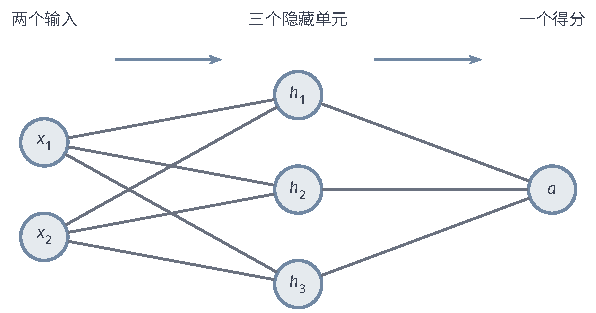
\includegraphics[width=100.993mm]{figures/05-neural-network-models/00-shared/tikz/neural-minimal-mlp/figure.pdf}
  \caption{一个$2$-$3$-$1$多层感知机：两个输入经过三个隐藏单元，得到一个分类得分。连线表示带权连接，箭头表示计算方向；隐藏单元作非线性变换，偏置未画出。}
  \label{fig:neural-minimal-mlp}
\end{figure}
\FloatBarrier

图中的每条连线都带有一个权重。以第一个中间单元为例，它先对两个输入作加权求和并加上自己的偏置，再把总和送入一个非线性函数（下一小节会说明为什么这一步不可或缺）：
\[
  a_1=w_{11}x_1+w_{21}x_2+b_1,\qquad h_1=\rho(a_1).
\]
另外两个单元$h_2,h_3$的算法完全相同，只是权重和偏置不同。于是，从同样两个计数出发，网络得到了三个新数字。输出单元再把这三个数字加权组合成分类得分：
\[
  s=v_1h_1+v_2h_2+v_3h_3+c.
\]
为获得具体感受，可以代入一组教学数值。假设$h_1$的权重为$w_{11}=1,w_{21}=-1$，偏置$b_1=0$，且$\rho(a)=\max\{0,a\}$（负的总和被截为零）。那么$h_1=\max\{0,x_1-x_2\}$只在“促销词数明显多于链接数”时才取非零值——这已经是一种关于两个特征\emph{搭配关系}的描述，尽管这里的权重是我们手填的。真实训练中，$w$、$b$、$v$、$c$都由梯度下降根据分类错误自动调整：如果某个中间单元的输出有助于降低错误，与它相连的权重就会朝相应方向改变，直到它稳定地检测某种对任务有用的模式。

这三个中间单元的数值不来自外界输入，也不直接作为最终答案，它们是网络内部的中间产物，因此称为\term{隐藏层}（hidden layer）。“隐藏”不是说它们不可观测，而是说它们的取值不构成训练数据：我们从不提供“$h_1$应该等于多少”的标签，只提供最终的垃圾邮件标签，让学习算法自己决定每个隐藏单元该检测什么。图中相邻两层之间两两相连、信息逐层向前流动，这种结构称为\term{多层感知机}（multilayer perceptron, MLP）。名字里的“感知机”源自早期的一种单层模型（见\ref{sec:neural-history-threshold}节），今天它已泛指这种由全连接层堆叠而成的网络。

需要强调的是，学习隐藏层不等于无中生有。网络只能重组输入中已经保留的信息：如果两封邮件被编码成完全相同的$(x_1,x_2)$，那么无论隐藏层多复杂，算出的$h_1,h_2,h_3$都相同，网络无法恢复编码阶段已经丢失的词序或上下文。因此，“让网络学习特征”并不取消输入编码的责任，而是把“该统计哪些组合”这一层决策，从人工提前固定改为在任务信号引导下从数据中形成。下一小节先从函数复合的角度说明这种改写为什么能增强能力。

\subsection{特征变换与函数复合}
\label{sec:neural-feature-composition}

表示变换的作用，是把输入改写到一个对任务更友好的坐标系中。仍以分类为例：线性分类器只能在输入空间中画一条直线（或一个超平面）作为两类的分界。若两类点在原坐标中犬牙交错，任何直线都分不开它们；但如果先把点映到一组新坐标，使正类聚在一起、负类聚在一起，在新坐标系中画一条直线就足够了。下面先给出形式化记号，再用一个最小例子展示这次“改写”的效果。

将可学习的表示变换记为$\bm{r}_{\bm{\theta}}(\bm{x})$，它把原始输入$\bm{x}$映为一个表示向量；再把利用表示产生预测的输出映射记为$g_{\bm{\psi}}$。整个网络就是两个函数的复合：
\begin{equation}
  f_{\bm{\theta},\bm{\psi}}(\bm{x})
  =g_{\bm{\psi}}\!\left(\bm{r}_{\bm{\theta}}(\bm{x})\right),
  \label{eq:neural-representation-readout}
\end{equation}
其中$\bm{\theta}$和$\bm{\psi}$分别是表示部分与输出部分的参数。在线性分类器中，表示是固定的（直接用$\bm{x}$），只有$g$的参数在学；神经网络中$\bm{\theta}$也在学，即“用什么坐标描述样本”本身成为学习对象。这种从数据中学习供后续任务使用的信息形式的做法，称为\term{表示学习}（representation learning）。

表示部分还可以由多层变换复合而成：上一层的输出作为下一层的输入，每层先作加权求和并加偏置，再通过一个\term{激活函数}（activation function）——一个逐元素作用的固定非线性函数，决定单元在多大输入下以多强的程度响应——作非线性变换。

\paragraph{为什么非线性不可省略。}
这是初学时最需要想清楚的一点。假设网络完全不使用非线性激活，两层的计算分别是
\[
  \bm{h}=\bm{W}_1\bm{x}+\bm{b}_1,\qquad
  \bm{s}=\bm{W}_2\bm{h}+\bm{b}_2.
\]
把第一式代入第二式：
\[
  \bm{s}=\bm{W}_2(\bm{W}_1\bm{x}+\bm{b}_1)+\bm{b}_2
       =(\bm{W}_2\bm{W}_1)\bm{x}+(\bm{W}_2\bm{b}_1+\bm{b}_2).
\]
令$\bm{W}=\bm{W}_2\bm{W}_1$、$\bm{b}=\bm{W}_2\bm{b}_1+\bm{b}_2$，两层网络就退化成$\bm{s}=\bm{W}\bm{x}+\bm{b}$——仍是输入的一个线性函数，与只有一层完全等价。重复同样的代入可知，任意多层线性变换的复合还是线性变换。这意味着：如果没有非线性，无论叠多少层，网络能画的分类边界仍然是一个超平面，深度不带来任何新能力。非线性激活的作用，正是打破这种可合并性，使每一层都可能把坐标系“弯折”到线性模型无法达到的形状。

\begin{example}[异或的表示变换]
  \label{ex:neural-xor-representation}
  \term{异或}（exclusive OR, XOR）要求：两个二值输入$x_1,x_2$不同时输出$1$，相同时输出$0$，即四个样本为
  \[
    (0,0)\mapsto 0,\quad (1,1)\mapsto 0,\quad (0,1)\mapsto 1,\quad (1,0)\mapsto 1.
  \]
  图~\ref{fig:neural-xor-representation}左侧可以看到，两个负例（圆点）处在对角线上，两个正例（方点）处在另一条对角线上，任何一条直线都无法把两类分开——这正是纯线性模型的失败情形。

  取\term{整流线性单元}（rectified linear unit, ReLU）激活函数$\rho(a)=\max\{0,a\}$，它把负值置零、正值原样保留。构造两个隐藏单元
  \begin{equation}
    h_1=\rho(x_1-x_2),\qquad h_2=\rho(x_2-x_1).
    \label{eq:neural-xor-hidden}
  \end{equation}
  逐个样本代入：
  \begin{equation*}
    \begin{array}{c|cc|c}
      (x_1,x_2) & h_1=\rho(x_1-x_2) & h_2=\rho(x_2-x_1) & \text{标签} \\ \hline
      (0,0) & 0 & 0 & 0 \\
      (1,1) & 0 & 0 & 0 \\
      (0,1) & 0 & 1 & 1 \\
      (1,0) & 1 & 0 & 1
    \end{array}
  \end{equation*}
  两个输入相同时，$(h_1,h_2)$都是$(0,0)$；输入不同时，其中一个坐标为$1$。在新坐标系中，两个负例重合于原点，两个正例落在坐标轴上，用一条直线$h_1+h_2=1/2$（图中虚线）就把两类分开了，输出端只需判断$h_1+h_2>1/2$。图~\ref{fig:neural-xor-representation}右侧画出了这次变换的结果。

  这个例子说明的是隐藏表示\emph{能够}完成什么：一次坐标变换把线性不可分的问题变成线性可分。但式中的权重是手工构造的，它并不证明训练算法在真实问题上必然能找到这样的参数——“能表达”和“能学到”是两件不同的事。
\end{example}

\begin{figure}[htbp]
  \centering
  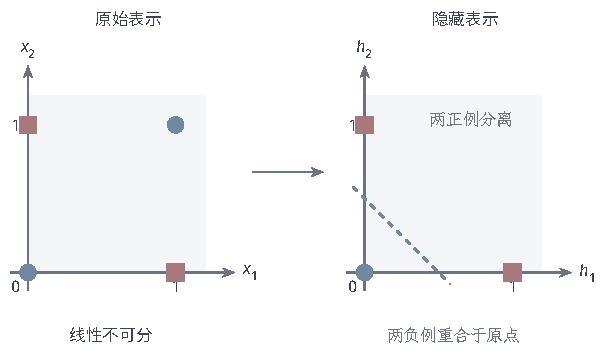
\includegraphics[width=102.902mm]{figures/05-neural-network-models/00-shared/tikz/neural-xor-representation/figure.pdf}
  \caption{异或任务的表示变换。圆点为负例，方点为正例。左侧无法用一条直线分开；按式\eqref{eq:neural-xor-hidden}变换后，右侧两个负例重合，虚线$h_1+h_2=1/2$将两类分开。坐标和变换均为教学构造。}
  \label{fig:neural-xor-representation}
\end{figure}

实际训练中，没有人手工给出隐藏层的目标值。学习算法先做一次前向计算得到预测，再用损失函数衡量预测与标签的差距，然后通过链式求导同时计算损失对$\bm{\theta}$和$\bm{\psi}$的梯度，一次性更新所有参数。这样，表示层的调整方向完全由“能否降低最终任务的损失”决定，无需为每个隐藏单元预先指定含义，这种训练方式称为\term{端到端学习}（end-to-end learning）——从原始输入到最终输出的整条映射作为一个整体接受同一个任务信号的训练。

由此必须区分三个常被混为一谈的问题。其一，\term{表示能力}（网络能不能表达完成任务所需的函数）：异或例子中的网络具备这种能力，但这只说明存在一组参数可行。其二，\term{优化}（训练算法能不能找到这组合适参数）：目标函数关于参数通常是非凸的，梯度下降可能停在较差的解。其三，\term{泛化}（学到的函数在未见样本上是否仍然有效）：在训练样本上把损失降到零，只说明记住了这些样本，不代表新样本也能正确处理。后续章节会反复回到这三个问题；本章只要求读者记住，肯定其中一个并不自动肯定另外两个。

\subsection{分布式表示与层次表示}
\label{sec:neural-distributed-hierarchical}

知道隐藏层能改造坐标后，进一步要问：多个单元、多层单元分别是怎样组织信息的？这两个问题对应两种相互正交的设计，理解它们有助于读懂后续所有架构图。

\term{分布式表示}（distributed representation）关注\emph{同一层内部}如何组织信息：一个对象由多个单元的活动共同表示，同一个单元又可以参与多个对象的表示。设想用三个单元分别编码“是否偏红”“是否圆形”“是否较大”，那么“红苹果”“红皮球”“青苹果”由这三个单元的不同活动组合区分，而不需要为每种物体单独分配一个单元。这种组织的好处是组合性：$k$个取值连续的单元可以形成大量不同的活动模式，识别一个新组合时也可能复用已有的各属性检测。需要澄清的是，实际网络中的隐藏坐标通常是连续数值，也未必分别对应某个可命名的属性；这里的“分布式”指信息分散承载在多个单元的联合活动中，与“多台计算机分布计算”无关\scite{goodfellow2016}

\term{层次表示}（hierarchical representation）关注\emph{不同层之间}如何组合信息：后一层把前一层的表示当作输入，在更高的抽象级别上构造新特征。以图像识别为例，第一层隐藏单元可能只响应局部的明暗突变（边缘小段）；第二层把相邻、方向一致的响应组合起来，得到对线条或拐角的检测；再往后组合成简单形状，直至与物体部件、整体物体对应的表示。后一层之所以能表示更复杂的东西，正是因为它建立在前一层已经提炼过的信息上。需要说明，层次表示描述的是这种逐层组合的关系，并不要求每一层都对应一个人类可命名的概念，也不保证层数越多表示就越有用——过深的网络在数据或训练方法不足时可能更难优化。

两种方式同时存在于一个网络中：每层内部用多个单元共同表示输入（分布式），层与层之间逐级组合这些活动（层次化），最终完成任务。图~\ref{fig:neural-representation-path}把这条路径画在一起：实线是预测时输入经各层变换得到输出的方向，虚线是训练时任务损失反向指导每一层参数调整的方向。

\begin{figure}[htbp]
  \centering
  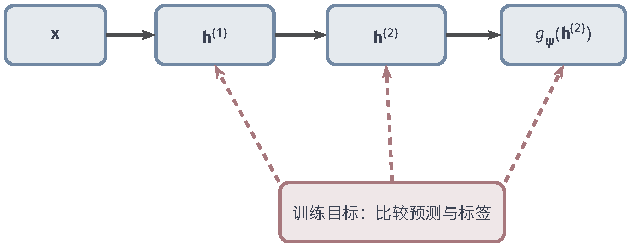
\includegraphics[width=106.793mm]{figures/05-neural-network-models/00-shared/tikz/neural-representation-path/figure.pdf}
  \caption{表示学习的计算路径。实线表示输入经各层变换得到预测，虚线表示训练目标指导表示层与输出层的参数调整。隐藏坐标无需具有预先指定的语义。}
  \label{fig:neural-representation-path}
\end{figure}

\subsection{结构带来的归纳偏置}
\label{sec:neural-structural-bias}

理论上，一个足够宽的多层感知机可以读取所有输入并让它们任意交互。那么为什么还需要卷积网络、循环网络这些专门结构？原因在于数据量和计算量都有限：若对所有任务都用全连接的通用网络，模型要么需要多得多的样本才能确定海量参数，要么在有限样本上学出不稳定的规律。如果我们事先知道数据中存在某些结构，把这种知识“写进”网络的连接方式，学习就会容易得多。

结构预先规定了两件事：哪些信息之间可以发生相互作用，哪些计算可以在不同位置或不同时刻重复使用。这些规定体现了模型对数据规律的假设。在有限样本下，任何能引导学习朝某类解收敛、并帮助模型推广到新样本的限制或偏好，统称为\term{归纳偏置}（inductive bias）。“偏置”在这里不是贬义的成见，而是学习能够发生的前提——没有任何偏好的模型面对有限数据无从选择。归纳偏置除了来自网络结构，也可以来自损失函数的形式或学习算法本身，这里主要讨论结构带来的偏置。

例如，图像数据有两条常见规律：有意义的模式通常由空间上相邻的像素构成，而同一种模式（如一条竖直边缘）可能出现在画面任何位置。针对前一条，\term{局部连接}（local connectivity）让每个单元只读取输入的一小块邻域，而不与整张图相连，强迫单元专注于局部模式；针对后一条，\term{参数共享}（parameter sharing）让同一组权重在图像的不同位置复用，使“在左上角学到的边缘检测”无需重新学习就能用于右下角。再如语言和语音这样的序列，当前判断往往依赖此前的内容，网络可以用一个\term{隐状态}（hidden state）——一个随处理过程不断更新的内部向量，可理解为网络递给下一步自己的“摘要便签”——保存由历史输入计算得到的信息，供后续时刻使用。

这些设计有助于利用数据中的规律、减少需要确定的参数量，但任何偏置都是双刃剑：它同时限制了模型能够表达的函数族。若任务本身不符合假设（例如强迫只看局部的网络判断需要全图布局的关系），偏置反而会妨碍学习。因此某种架构表示能力强，不等于它必然容易训练或一定泛化得好，结构是否合适需要结合任务判断。关于表示能力的形式化结论，可参考\BookChapterRef{chap:deep-learning-theory}{卷3《基础、理论与可信性》的“深度学习的可学习性”章}。

\section{生物神经网络}
\label{sec:neural-biological-inspiration}

神经网络的名字和术语大量借用自神经科学：“神经元”“连接”“学习”“激活”。这些类比是历史形成的——早期研究者确实希望用电路模拟智能——但今天工程上有效的神经网络，其数学与真实神经系统的差距已经很大。本节按三条线索梳理这种关系：单个神经细胞如何通信（\ref{sec:neural-biological-unit}节）、大量细胞如何组成处理系统（\ref{sec:neural-biological-system}节）、经验如何改变连接（\ref{sec:neural-biological-learning}节），最后在\ref{sec:neural-biological-comparison}节对照人工单元与人工网络，说明哪些相似是实质性的功能抽象，哪些只是名词借用。

\subsection{神经元}
\label{sec:neural-biological-unit}

生物\term{神经元}（neuron）是神经系统中接收、处理和传递信号的细胞。一个典型神经元分为三部分：大量树突负责从其他细胞接收信号，胞体进行整合，一根轴突把信号传给其他细胞。输入信号会改变细胞膜内外带电离子的浓度差，即\term{膜电位}（membrane potential）。单个输入通常很微弱，胞体把来自许多连接、在不同时刻到达的影响累加起来：当膜电位升高到某个阈值附近，细胞就触发一次\term{动作电位}（action potential）——一个持续约一毫秒、沿轴突主动传导的短暂电脉冲，也称“发放一次”；脉冲过后膜电位恢复，细胞经过短暂不应期才能再次发放。轴突末梢与下一个细胞的树突或胞体之间有微小间隙，这个传递影响的连接部位称为\term{突触}（synapse）。图~\ref{fig:neural-biological-neuron}展示一个细胞通过轴突分支向另外两个细胞传递信号的结构\scite{purves2001}

\begin{figure*}[!t]
  \centering
  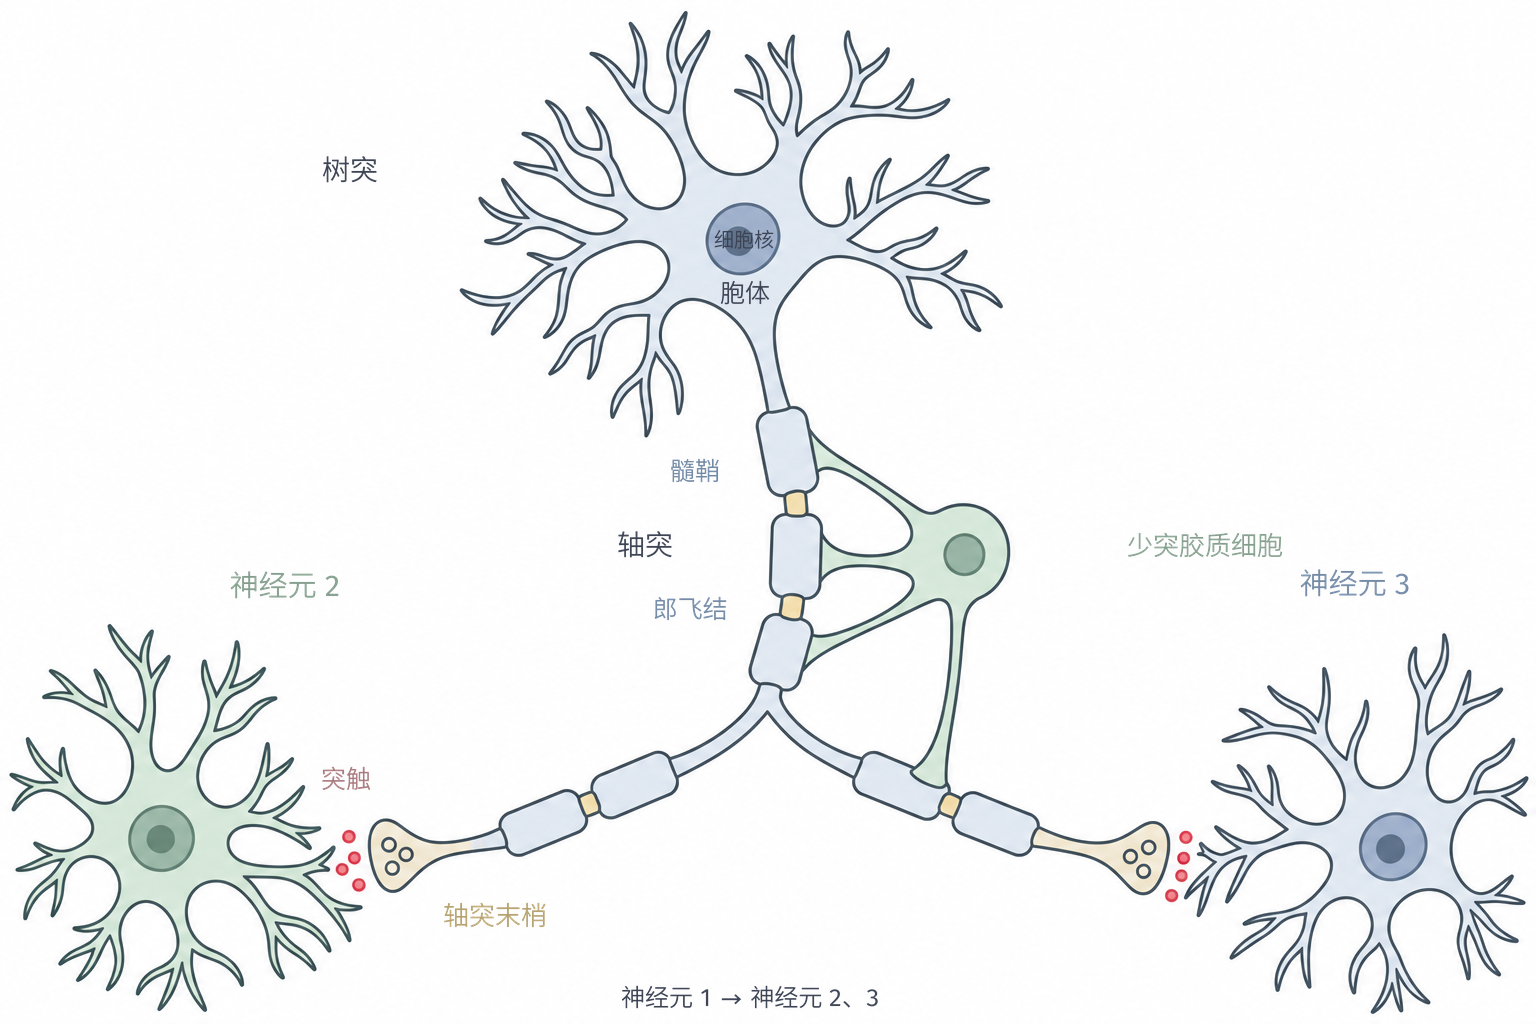
\includegraphics[width=130.048mm]{figures/05-neural-network-models/00-shared/generated/neural-biological-neuron/figure.png}
  \caption{三个神经元通过突触相连。神经元1的轴突分支分别联系神经元2和3，表示一个细胞可以影响多个细胞。图示一种有髓鞘的多极神经元形态，髓鞘段之间的间隙为郎飞结；各部分不按比例，真实神经元形态多样，并非所有轴突都有髓鞘。}
  \label{fig:neural-biological-neuron}
\end{figure*}

在最常见的化学突触中，脉冲到达轴突末梢会促使末梢释放神经递质，递质扩散过间隙、改变接收细胞膜上的离子通道，从而升高或降低它的膜电位。因此一个突触的作用可能是\emph{兴奋性}的（促进接收细胞发放），也可能是\emph{抑制性}的（压低发放倾向），并不保证“来一个输入就产生一个脉冲”。是否发放取决于许多突触输入与细胞当前状态的共同整合：不仅输入的数量和强弱有关，到达的时间排布也有关——同样数量的脉冲，密集到达可能越过阈值，分散到达则可能在恢复中相互抵消。正因为真实细胞的响应同时依赖输入内容、时间和内部状态，它无法被“固定权重的静态加权和”完整描述；人工单元（见\ref{sec:neural-biological-comparison}节）保留的只是“多输入整合后决定输出”这一层抽象\scite{gerstner2014}

\FloatBarrier
\subsection{神经系统}
\label{sec:neural-biological-system}

单个细胞的发放不足以解释看、记、动作这些整体功能。神经元先在局部组成回路，回路之间再通过有组织的长距离纤维束连接，形成分工协作的脑区系统。一个脑区的活动取决于它接收的输入、区内细胞的连接方式、当前的兴奋或抑制状态，以及从高级区域返回的反馈连接；因此神经元的数量本身不能直接换算成计算能力，连接的组织方式同样关键\scite{purves2001}

以研究得最充分的视觉为例，图~\ref{fig:neural-visual-pathways}概括了一条主要通路：光线在视网膜被转换成神经信号，经丘脑的外侧膝状体（LGN）中继，到达大脑后部的初级视觉皮层（V1），再向更高皮层区域发散。之后大致形成两条分工不同的通路：\term{腹侧视觉通路}（ventral visual stream）向颞叶延伸，偏重处理颜色、形状和物体身份，常被称为内容通路what；\term{背侧视觉通路}（dorsal visual stream）向顶叶延伸，偏重运动、空间关系和视觉引导的动作，常被称为空间通路where。这种分工在日常动作中可以直接体会：看到桌上的杯子时，“认出它是杯子”（是什么）与“判断杯子的位置、控制手伸过去并张开合适的角度”（怎样抓）由不同但相互配合的信息支持。真实视觉系统还包含大量跨通路联系和从高级区域返回低级区域的反馈，并非一次从前往后的单向传递\scite{purves2001,goodale1992}

\begin{figure*}[!t]
  \centering
  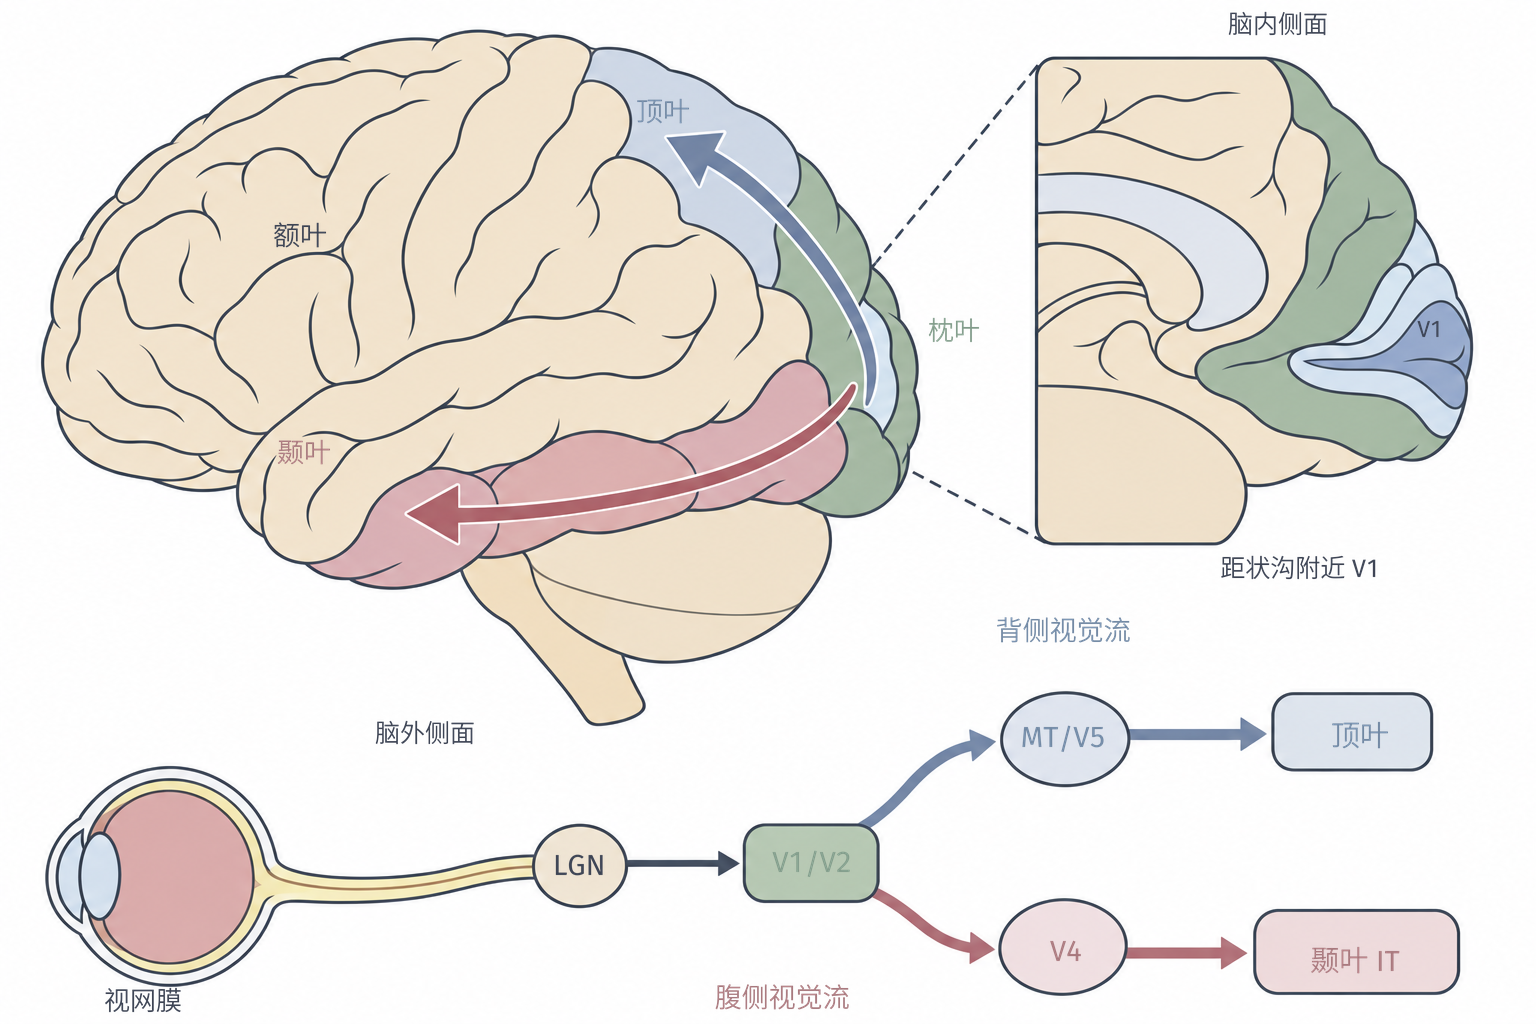
\includegraphics[width=130.048mm]{figures/05-neural-network-models/00-shared/generated/neural-visual-pathways/figure.png}
  \caption{人脑视觉区域与主要通路示意。视觉信号从视网膜经LGN进入V1/V2；蓝色分支经MT（V5）向顶叶传递空间与运动相关信息，红色分支经V4向下颞皮层IT传递物体相关信息。解剖图用于定位，箭头不表示精确边界、完整连接或唯一串行顺序，跨通路联系与反馈未画全。}
  \label{fig:neural-visual-pathways}
\end{figure*}

视觉系统中的一个关键概念是\term{感受野}（receptive field）：一个视觉神经元只受到视野中某一块有限区域内光刺激的影响，这块区域就是它的感受野；刺激落在感受野外，该神经元基本不响应。Hubel和Wiesel在20世纪60年代对猫视觉皮层的经典实验中发现，V1及附近区域的许多细胞并不对均匀光斑反应，而对特定取向、位置的局部光条有选择性，越往高级区域，细胞响应的模式越复杂、感受野越大。这种“先由局部检测、再逐层组合成复杂模式选择性”的组织方式，为人工网络的层次表示（见\ref{sec:neural-distributed-hierarchical}节）和卷积结构提供了生物学线索；但这只是原理层面的启发，不能据此认为某个人工计算层对应某个具体脑区\scite{hubel1962,purves2001}

\FloatBarrier
\subsection{生物学习}
\label{sec:neural-biological-learning}

前面描述的是神经系统在某一时刻如何响应。学习还要求回答另一个问题：经验怎样改变神经系统，使它今后的响应不同？

生物学习的物质基础发生在突触上。\term{突触可塑性}（synaptic plasticity）指突触传递效果能够随神经活动等因素持续改变——同一个突触，在特定的活动经历之后可能变强或变弱，而且这种改变可以保持一段时间。最有影响的一类概括称为\term{赫布学习}（Hebbian learning），常被通俗概括为“一起发放的细胞连得更紧”：如果突触前后两个神经元倾向于在相近时刻共同活动，这个突触的传递效果倾向于增强。它的直觉是把“反复同时出现”当作“两者相关、值得加强联系”的证据。后续研究进一步发现，活动的\emph{先后次序}也很关键：\term{脉冲时序依赖可塑性}（spike-timing-dependent plasticity, STDP）描述这样一类现象——突触前细胞略早于突触后细胞发放时，突触倾向于增强（前者像是后者发放的原因）；次序相反时则倾向于减弱。需要注意，STDP的具体方向和幅度受细胞类型、突触初始状态和实验方案影响，不存在所有突触统一遵守的一条规则\scite{bi1998,gerstner2018plasticity}

局部突触规则解释了连接如何随邻近活动改变，但学习的目的是改善整体行为，两者之间还隔着一个难题。练习伸手抓杯子时，如果这一次抓偏了，这个“偏差”是在动作末端才知道的；参与的神经元却遍布视觉、规划和运动控制的整条回路。究竟应该让回路中的哪些突触变强、哪些变弱，才能让下一次抓得更准？这就是\term{信用分配}（credit assignment）问题：整体结果应当如何追溯并影响内部各个环节。仅凭“两端一起发放”无法确定某条具体连接对这次行为偏差贡献了多少；大脑中可能由弥散的调节信号、反馈连接和多时间尺度的可塑性共同参与，但具体机制仍是开放的研究问题\scite{lillicrap2020}。这个问题在人工网络中同样存在，而工程上给出的答案（反向传播）将在\ref{sec:neural-biological-comparison}节末尾对照。

\subsection{与人工神经网络的对比}
\label{sec:neural-biological-comparison}

现在可以精确地说明人工单元从生物神经元那里保留了什么。对于输入向量$\bm{u}\in\mathbb{R}^{d}$，一种最常见的人工单元计算
\begin{equation}
  a=\sum_{j=1}^{d}w_j u_j+b,\qquad h=\sigma(a),
  \label{eq:neural-artificial-unit}
\end{equation}
如图~\ref{fig:neural-unit-abstraction}所示：各输入$u_j$乘以对应的权重$w_j$（对应突触可强可弱、可正可负的影响），求和后加偏置$b$（对应细胞固有的发放倾向），再经激活函数$\sigma$得到输出$h$（对应“整合后是否、以多强程度响应”）。这一公式保留的是功能层面的对应——接收多路输入、整合影响、产生输出；它没有复现脉冲的离散发放、抑制性与兴奋性递质的化学差异、膜电位的时间动态和各种不应期。生物神经元更像一个复杂的非线性时变系统，而式\eqref{eq:neural-artificial-unit}是一个静态的数学单元。

\begin{figure}[!t]
  \centering
  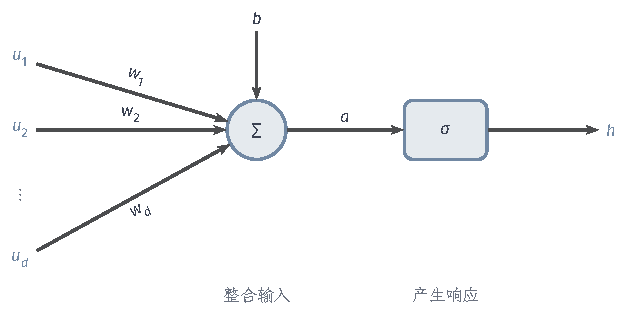
\includegraphics[width=106.161mm]{figures/05-neural-network-models/00-shared/tikz/neural-unit-abstraction/figure.pdf}
  \caption{人工单元先将各输入乘以权重，求和并加入偏置，再经激活函数产生输出。它保留接收、整合与输出的功能对应，数学运算不完整复现生物细胞。}
  \label{fig:neural-unit-abstraction}
\end{figure}

把多个单元连接起来后，比较的对象就从细胞上升为网络。图~\ref{fig:neural-biological-artificial-networks}将两者并置：真实神经回路中既有细胞类型的差异，也有局部小回路、跨区域长连接和大量反馈联系，信息往往在环路中反复流动；右侧的典型层状前馈网络则按人为规定的计算依赖，从输入经若干中间层一次性得到输出。当然，人工网络也可以加入环式连接（循环网络）和内部状态，因此不能笼统地断言“大脑有反馈而人工网络没有”——两者的比较必须落实到具体结构，更不能用节点数量简单类比。

\begin{figure*}[!t]
  \centering
  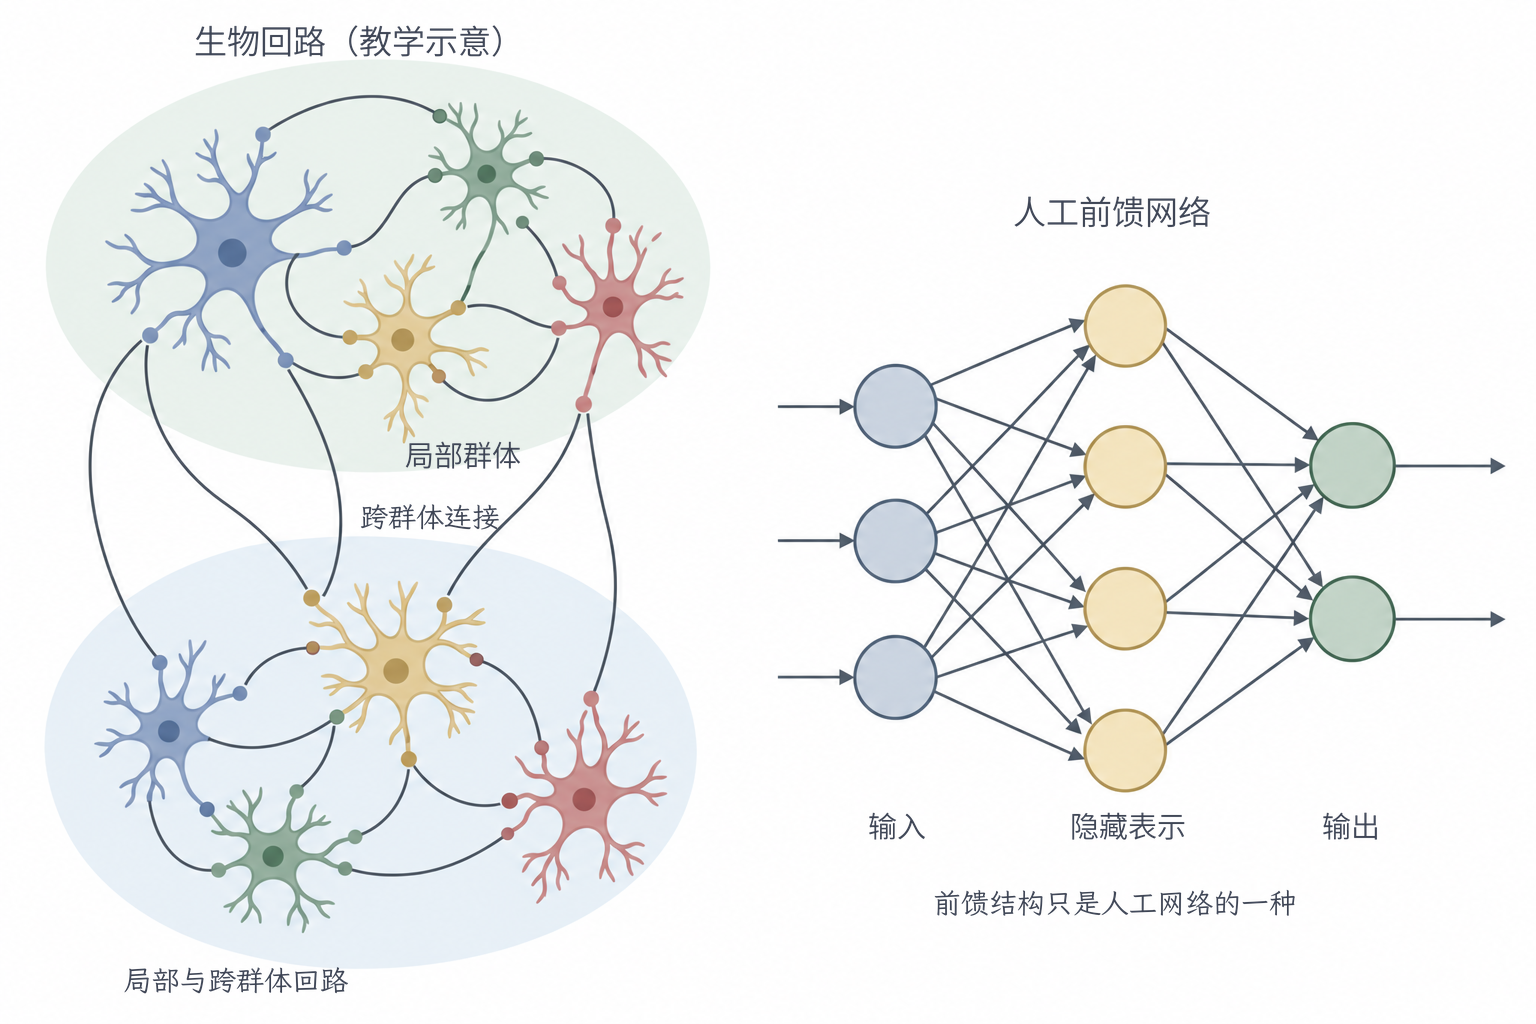
\includegraphics[width=130.048mm]{figures/05-neural-network-models/00-shared/generated/neural-biological-artificial-networks/figure.png}
  \caption{生物回路与前馈人工网络的组织示意。左侧表示细胞差异、局部群体及跨群体联系，是教学构造；右侧箭头表示输入、中间表示与输出的计算依赖。节点数量不表示真实规模，右图不涵盖所有人工结构。}
  \label{fig:neural-biological-artificial-networks}
\end{figure*}

视觉机制的生物学发现确实多次启发了人工结构。\term{新认知机}（neocognitron）交替组织局部模式检测与响应汇集，使识别对一定范围内的位置变化更容忍\scite{fukushima1980}卷积网络沿用局部连接与参数共享组织图像计算，其中参数共享更多是出于效率和统计考虑的工程约束，而非对生物事实的复刻；脉冲网络则选择保留“发放事件及其精确时间”这一维度（见本卷脉冲网络章）。它们分别借鉴了生物系统的不同侧面，没有一个试图复制全部机制。

在“学习”这一点上，两类系统的共同点是经验能够改变连接强度，更新依据却可以完全不同。标准的\term{误差反向传播}（error backpropagation）先完成一次前向计算，再利用整体任务损失对每个参数求梯度，让输出端的错误逐层传回每一条连接；赫布规则、STDP这类局部规则则只根据一个突触两端的活动决定变化，不直接知道整体行为的好坏。目前关于生物反馈通路和可塑性的研究，尚不能证明大脑执行的是标准反向传播；反过来，人工网络也不排斥使用局部学习规则\scite{lillicrap2020}。因此选择单元形式、连接方式、信号编码和学习规则时，应当服从模型要解释的现象或要完成的任务，而不以“是否更像大脑”为标准。

\section{神经网络的类型}
\label{sec:neural-network-types}

经过前面的讨论，我们已经可以凭直觉描述网络：输入经过若干层非线性变换得到输出，层间连接可以遵循各种结构假设。但打开任何一篇论文都会遇到一大堆名字：卷积网络、循环网络、图网络、Transformer、脉冲网络、注意力网络……新手常误以为它们是一张互斥清单上的并列选项。事实上，这些名字强调的是网络的不同侧面。本节给出三个相互独立的判断维度：计算依赖如何组织（\ref{sec:neural-types-connectivity}节）、信息以什么方式交互（\ref{sec:neural-types-interaction}节）、单元用什么形式的信号承载信息（\ref{sec:neural-types-encoding}节）。同一个具体网络通常可以在三个维度上分别被描述，三个维度的回答可以自由交叉；读完本节后应能回答：“卷积网络能不能是循环的？”“图网络和前馈网络矛盾吗？”这一类问题。

\subsection{按连接结构划分}
\label{sec:neural-types-connectivity}

这一维度考察的是\textbf{层或模块之间的连接是否形成有向回返}，即计算中是否存在一条从某单元出发、沿箭头又回到该单元的路径。

\term{前馈神经网络}（feedforward neural network）的层间依赖不包含任何有向环：信息从输入出发，沿依赖关系单向流向输出，每个单元只被计算一次。允许跨层的跳接（让某层直接读取更早层的输出），只要不构成回返，网络仍是前馈的。\term{循环神经网络}（recurrent neural network, RNN）则把前一次计算留下的内部状态用于下一次更新：当前输出不仅取决于当前输入，还取决于上一步保存下来的状态；由于状态在时间步之间反复读写，展开来看就形成了环。循环网络通常在多个时间步复用同一组更新参数。

用同一个句子分类任务可以看清差异。对“这部电影并不好看”这样的评论，前馈网络需要先把整句整理成一个定长向量，再一次性读取它作出判断；循环网络则逐词读入，读到“不”时状态发生改变，这个改变后的状态继续参与读到“好”“看”时的计算，于是否定关系有了一条自然的表达路径。需要特别注意两点区分依据：判断前馈还是循环，看的是\emph{状态是否在计算步骤之间传递}，而不是“输入是不是序列”——前馈网络也可以处理序列（只要序列被预先整理成定长表示）；也不是“参数是否共享”——共享参数本身不构成环。循环更新按时间展开后，每个时间步内部仍是按先后顺序的普通计算，所以它并不神秘，只是把同一个计算重复施加在“输入+此前状态”上。

树形和图形数据描述的是另一种结构特征，它们回答“输入对象本身有没有内部关系结构”，与有没有环是两回事。\term{树递归网络}（recursive neural network）按父子关系递归组合表示，例如把句子的短语结构分析成树，先组合子短语的表示，再由子短语形成整句表示。\term{图神经网络}（graph neural network, GNN）则直接利用输入中实体之间的关系，例如把路口网络建模为图，路口是节点、道路是边，每个节点的新表示由其道路相连的邻居聚合而成。关键在于：即使输入图本身带有环（城市道路中随处可见的环路），网络也可以规定“每一层只读取上一层留下的表示”，于是一次更新内部的信息流向仍然是前馈的。因此“图网络”并不是与“前馈、循环”并列互斥的第三类：它说的是计算沿输入给定的关系结构进行，而前馈/循环说的是这些计算依赖本身有没有回返。此外，\term{状态空间模型}（state space model, SSM）用一个连续的内部状态概括历史，再由状态读出输出，是循环思路的另一种常见数学形式。

图~\ref{fig:neural-topologies}分别展示无回返的前馈依赖、循环更新沿时间展开后的形态，以及按输入图读取邻居的一次聚合。任何网络最终都能画成一张由节点和箭头构成的计算图；“图神经网络”特指\emph{利用输入数据自带的关系结构}来组织表示的模型，而不是泛指所有“长得像图”的网络。
\begin{figure}[htbp]
  \centering
  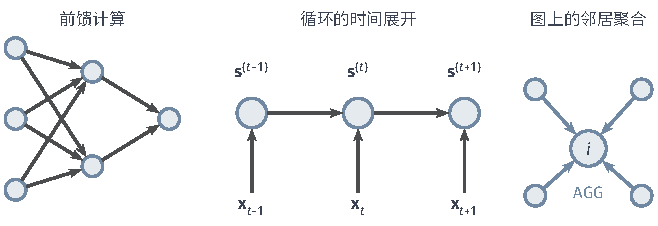
\includegraphics[width=111.361mm]{figures/05-neural-network-models/00-shared/tikz/neural-topologies/figure.pdf}
  \caption{三种结构视角。左侧为无回返的前馈依赖；中间为循环更新的时间展开，各步共享状态更新参数；右侧为图网络的一次邻居聚合，邻居向中心节点$i$提供信息。输入图的环不等于一次更新中的计算循环。}
  \label{fig:neural-topologies}
\end{figure}
\FloatBarrier

\subsection{按信息交互方式划分}
\label{sec:neural-types-interaction}

确定计算依赖的大框架后，下一个问题是：当一个单元要综合多个来源的信息时，它\textbf{能读取多大范围、来源关系由谁决定、各个来源的权重如何形成}？常见机制正是在这三点上不同；它们不是互斥类型，而常常出现在同一个网络的不同层中。

\term{全连接}（fully connected）让每个输出单元读取上一层的全部坐标，每条连接都有一个独立的、待学习的权重。\term{卷积}（convolution）通常作用于规则网格（如图像像素），每个单元只读取一个局部邻域，而且同一组权重在网格的所有位置复用。仍以边缘检测为例：一条竖直边缘无论出现在左上角还是右下角，在统计上是同一种局部模式，用同一组权重检测即可，无需为每个位置单独学一份。二者的差别可以归结为“一次读取的范围”和“权重是否跨位置共享”；它们都可以放在前馈网络中，一个卷积网络的末端也常接全连接层，因此“卷积还是全连接”是针对\emph{层}的提问，不是针对整个网络的非此即彼。

当输入的关系不规则时，读取范围可以直接由输入关系给出。\term{消息传递}（message passing）按输入图确定每个节点可以读取的来源——它的邻居——再把邻居发来的信息聚合起来；不同节点的邻居数量不必相同，正如每个路口相连的道路数不同。另一种机制改变的是权重的形成方式。\term{注意力机制}（attention mechanism）不让权重固定，而是根据当前表示，临时计算各信息来源在\emph{这一次}组合中应占的份额。用交通网络作比：消息传递回答“我听哪些路口”（由道路连接决定，固定不变），注意力回答“这次我更该听谁”（取决于当前路况，随内容变化）。同一个路口节点可以在按邻居聚合的同时，用注意力给各邻居分配动态权重，两种机制天然可以叠加。注意力的读取范围也不必是全体单元，可以限定在一个局部窗口或图邻居内，使用注意力并不意味着所有单元必须彼此相连。

注意力同样可以用于序列中各位置之间的交互，但允许读取哪些位置仍要根据任务规定：对一个完整句子作编码时，每个词都可以读取整句的上下文；而在逐步续写时，当前位置不能读取尚未生成的后续内容，否则等于偷看答案。还要区分两种“权重”：随每次输入变化的是注意力的组合系数（由当前内容临时算出），而网络中待训练的参数（决定“如何计算这些系数”的那些权重）是固定的、不会在一次预测中被重新训练。\term{Transformer}以注意力组织位置间交互，同时每个位置还配有独立的前馈变换；卷积或循环网络也可以在某些层插入注意力模块。因此判断一个模块的交互方式时，应直接考察该模块读取范围、关系来源和系数形成方式，而不能用整个架构的名字代替分析。

\subsection{按信息编码方式划分}
\label{sec:neural-types-encoding}

第三个维度考察的是\textbf{单元之间传递的信号本身}：是连续数值，还是离散的发放事件。

\term{连续值激活}（continuous-valued activation）用数值的大小承载信息：单元的输出是一个实数，数值越大通常表示响应越强，前面各节的网络都采用这种方式。这里的“连续值”是数学模型层面的描述；在计算机中任何数值都以有限精度存储，这不影响模型语义。

\term{脉冲神经网络}（spiking neural network, SNN）则模仿生物神经元，以离散的发放事件传递信息：单元在大部分时间沉默，只在特定时刻发出脉冲。信息可以编码在多个方面——一段时间内发放的脉冲数量（发放越密集表示响应越强）、脉冲发放的精确时刻，或多个单元脉冲之间的相对时序。这里需要区分对外信号与内部状态：单元向外发送的是离散脉冲，但它内部的膜电位等状态变量仍可取连续值并随时间连续演化；“脉冲网络是二值网络”是常见误解。

编码方式与前两个维度彼此独立：脉冲网络可以用卷积组织空间连接，可以是前馈的，也可以带循环连接；一个层间前馈的脉冲网络，单元内部仍可保留对历史的电位记忆。脉冲事件式的通信在生物学上更真实，在特定低功耗硬件上也可能因为“大部分单元大部分时间不活动”而节省能耗，但是否真的节能，还需结合活动密度、运行时间和具体实现条件综合评价，不能仅凭“脉冲”二字断定。

表~\ref{tab:neural-cross-classification}把三个维度的回答交叉起来。可以看到，一个带注意力的循环网络在连接组织上递推状态、在交互方式上按内容动态聚合、在编码上仍用连续值；而前馈脉冲卷积网络同时具备层间前馈、局部共享和脉冲事件三种性质。每一列回答的是不同问题，记住这一点，面对新架构名称时就知道该把它拆到哪些维度上理解。
\begin{table*}[htbp]
  \centering
  \small
  \begin{tabularx}{\linewidth}{@{}>{\RaggedRight\arraybackslash}p{45mm}>{\RaggedRight\arraybackslash}p{42mm}>{\RaggedRight\arraybackslash}X>{\RaggedRight\arraybackslash}p{26mm}@{}}
    \toprule
    \textbf{代表形式} & \textbf{连接组织} & \textbf{主要交互} & \textbf{信号编码} \\
    \midrule
    层状全连接网络 & 层间前馈 & 稠密加权组合 & 连续值激活 \\
    前馈卷积网络 & 层间前馈 & 局部连接与参数共享 & 连续值激活 \\
    带注意力的循环网络 & 状态递推 & 状态更新与动态聚合 & 连续值激活 \\
    固定轮数的图消息传递网络 & 按轮次展开 & 按输入图聚合邻居 & 连续值激活 \\
    前馈脉冲卷积网络 & 层间前馈，单元保留状态 & 局部连接与参数共享 & 脉冲事件 \\
    \bottomrule
  \end{tabularx}
  \caption{同一网络可以按连接组织、交互机制和信号编码分别描述。表中是展示交叉关系的代表形式，不穷尽同名网络的变体。}
  \label{tab:neural-cross-classification}
\end{table*}

\FloatBarrier

\section{神经网络的历史}
\label{sec:neural-history}

神经网络常给人“突然爆发”的印象，但它的主要思想是在几十年里围绕三个相互联系的问题逐步展开的：第一，怎样用相互连接的简单单元\emph{表达}计算（结构问题）；第二，连接中的参数怎样从经验中\emph{获得}（学习问题）；第三，在有限的数据和计算条件下怎样\emph{用得起}这些网络（规模问题）。历史中的代表性工作，分别在这三个环节上移除了一个具体障碍。图\ref{fig:neural-network-history}与图\ref{fig:neural-network-history-recent}按时间展示代表工作，年份采用论文发表或首次公开时间。阅读时请保持两个意识：这些机制解决的是不同环节的问题，因而大多可以组合使用，时间先后不表示“后者淘汰前者”；许多思想都经历过早于流行年份的铺垫，本节标注的是形成广泛影响的代表工作。

% 历史图分别随早期与近期机制说明排布，保留可读字号并为相关正文留出空间。
\Needspace{10\baselineskip}
\subsection{从阈值单元到可学习网络}
\label{sec:neural-history-threshold}

最早的问题是：相互连接的简单单元，原则上能完成什么计算？1943年，McCulloch和Pitts给出了一种理想化的二值神经元：每个单元对若干二值输入加权求和，再与固定阈值比较，决定输出$0$或$1$；通过合适地安排连接，网络可以实现各种逻辑组合。这个模型的意义在于第一次形式化地说明“神经元式的网络可以执行逻辑计算”，但它的权重和阈值全部由设计者手工指定，网络本身并不学习，因此它还不是现代意义上的机器学习模型\scite{mcculloch1943}

如果权重能够随经验改变，网络就有机会自己从样本中归纳分类规则。Rosenblatt在1958年提出的感知机（perceptron）把这一步走了出来：基础形式对输入加权后按阈值输出类别，并在每次预测错误后，按错误方向小幅调整相应权重——把判错的正样本相关权重调高、判错的负样本相关权重调低，规则简单到可以用电硬件实现，在当时引起轰动。需要说明，Rosenblatt的原始体系包含感觉单元、联想单元和反应单元等更丰富的组织，不应把其中所有形式都等同于今天教科书里的单层线性分类器\scite{rosenblatt1958}

热情随后遇到了能力边界。Minsky和Papert在1969年分析指出，没有隐藏层的感知机只能学习线性可分的函数，示例~\ref{ex:neural-xor-representation}中的异或就是它无法解决的最简单反例。这个批评的实质不是“神经元式计算行不通”，而是指出了单层的局限；而当时虽然知道加入隐藏单元可以扩大可表达函数的范围（异或例子已证明这一点），却没有一个被广泛认可的、能决定隐藏层权重的训练算法——隐藏单元没有自己的标签，谁来告诉它们该学什么？这个信用分配难题使神经网络研究进入了一段相对低潮，直到有效的多层训练方法出现。

\begin{figure*}[!t]
  \centering
  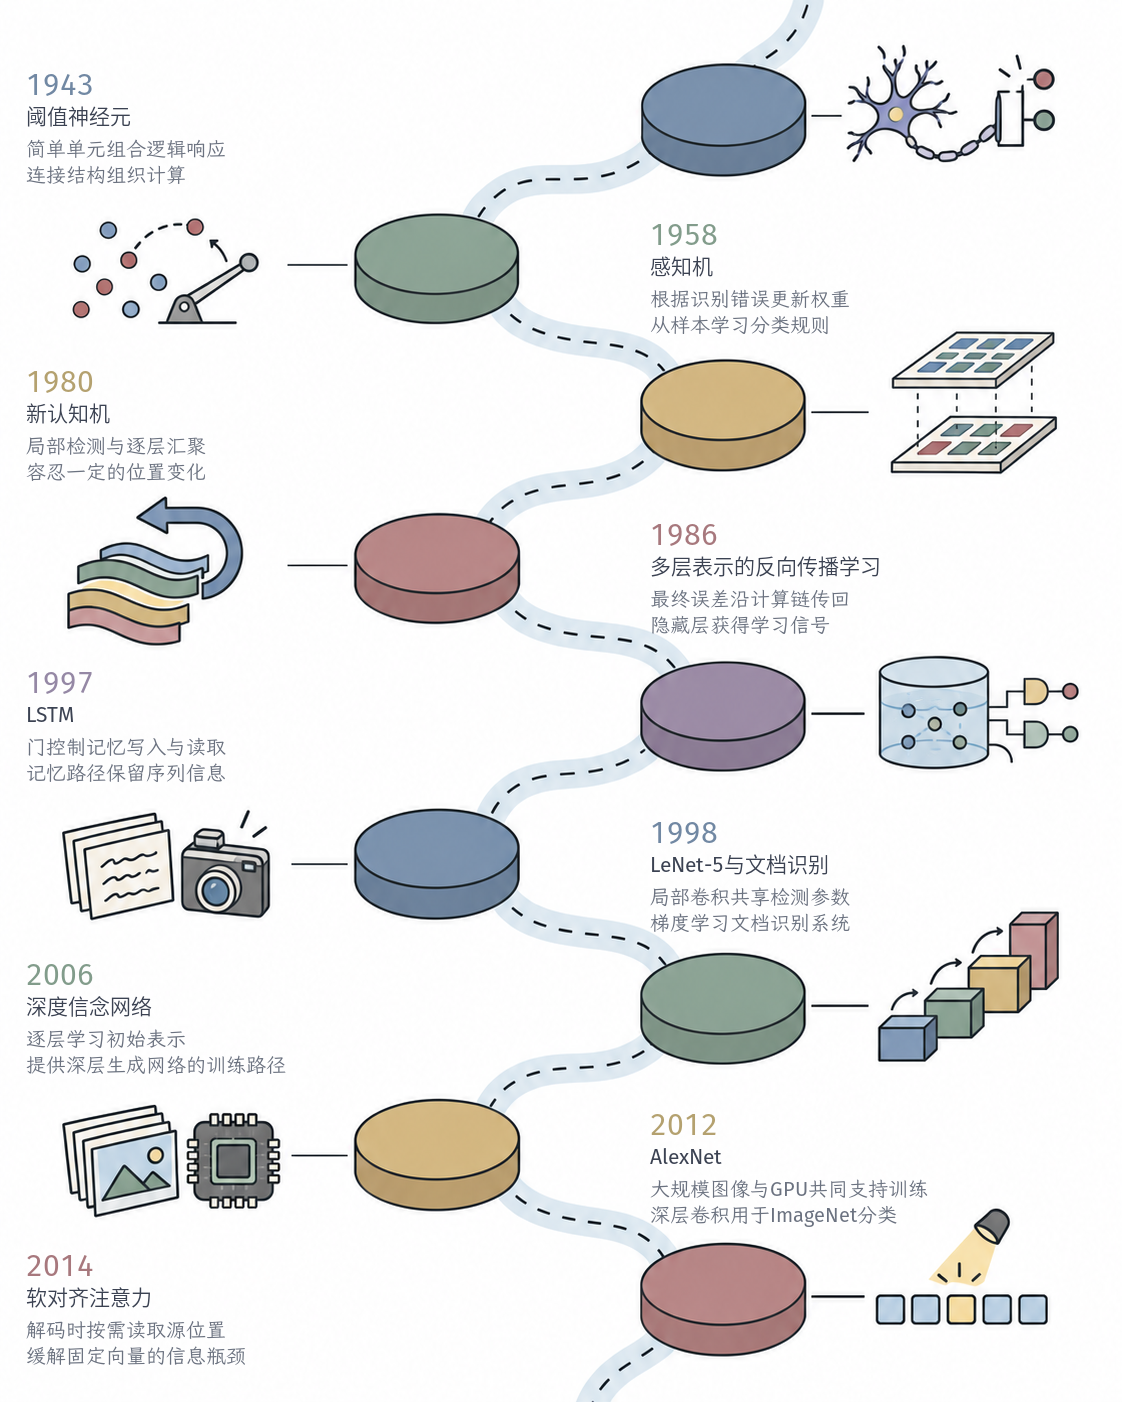
\includegraphics[width=149mm]{figures/05-neural-network-models/00-shared/generated/neural-network-history/figure.png}
  \caption{神经网络发展的代表工作（1943—2014）。沿虚线路线从上向下阅读，文字指出各项工作改变的计算或学习机制。年份采用代表论文的首次公开或发表时间；节点间距不按时间比例绘制，先后不表示替代。}
  \label{fig:neural-network-history}
\end{figure*}

\subsection{从浅层学习到深层训练}
\label{sec:neural-history-deep-training}

要让隐藏层参与学习，输出端的错误必须能转化为对每个内部参数的调整量。微积分其实已经提供了工具：复合函数可以用链式法则逐层求导。1986年，Rumelhart、Hinton和Williams系统展示了用误差反向传播训练多层网络的方法——先前向计算预测和损失，再沿计算的反方向逐层求出损失对每个参数的偏导，配合梯度下降更新。这使“没有标签的内部单元”第一次有了明确的学习信号：它的梯度由它对后续层、最终对损失的贡献决定。反向传播成为多层表示学习的代表性起点，但链式求导本身是已有数学工具，相关思想在不同领域也有更早的探索，不应把1986年当作一切相关算法的统一起点\scite{rumelhart1986}

学习规则之外，结构可以直接利用任务中的先验规律。1980年的新认知机已经用局部特征检测和逐层汇聚研究位置变化下的识别，不过它采用的是自组织式学习，不同于后来的监督梯度训练\scite{fukushima1980}卷积网络把局部连接、参数共享与反向传播结合：同一种局部模式检测在所有位置复用，既大幅减少参数，又契合图像统计规律。LeCun等人1998年用于手写文档识别的LeNet，展示了这种结构与基于梯度的整体训练结合后的实际效果\scite{lecun1998}

序列任务提出了另一个问题：如何让很久以前的输入影响当前输出？普通循环网络在时间维度上反复应用同一函数，相当于一个很深的复合结构，反向传播时梯度在连乘中容易逐层衰减或放大，远处信息的影响和它对应的学习信号都可能消失。Hochreiter和Schmidhuber在1997年提出的\term{长短期记忆}（long short-term memory, LSTM），为信息增设了一条受门控的“记忆通道”：输入门、遗忘门和输出门这些可学习的开关决定哪些新信息写入、哪些旧信息保留、哪些内容读出，使网络有可能跨越很多时间步维持信息。它为长期依赖提供了更合适的计算路径，但门控只是\emph{允许}信息长期保存，实际能学到多长的依赖仍取决于训练设置和数据\scite{hochreiter1997}

在反向传播已可用之后，深网络一度仍然难训，逐层预训练提供了一条过渡路径。2006年的\term{深度信念网络}（deep belief network, DBN）用多层潜变量描述数据的生成过程，即建模“可能观测到的数据”的概率分布；训练时先无监督地学好一层，再把这层的表示当作下一层的输入继续学习，逐层堆叠后再整体微调。它证明了深层结构是可以训练的，并推动了深度生成模型的发展，但这条路线不同于直接按分类损失端到端训练所有层\scite{hinton2006deepbelief}

真正让深层网络在主流任务上展现压倒性效果的，是数据、计算与结构三者的汇合。2012年的AlexNet在ImageNet大规模图像分类竞赛中大幅领先传统方法：它依赖上百万张带标注图像、用图形处理器（graphics processing unit, GPU）承担原本难以负担的并行训练计算，并配合了ReLU激活、 dropout正则化等结构与训练设计。这项成果说明的是配合效应，而不是“层数越多越准”的简单结论\scite{krizhevsky2012}。网络继续加深后又出现新的优化困难：层数过多时，梯度路径过长，训练误差反而可能上升。\term{残差连接}（residual connection）给出的办法是，在维度相容时让输入通过一条“直达通路”与若干层变换的结果相加：$\bm{x}_{\text{out}}=\bm{x}+F(\bm{x})$，于是中间层只需学习“在已有表示上还要补充的变化”$F$，梯度也可以沿直达通路传回。残差网络使训练上百层的网络成为可能；卷积、门控记忆和残差连接改变的是不同环节，因此可以在同一模型中配合使用\scite{he2016resnet}

\subsection{从固定连接到内容相关计算}
\label{sec:neural-history-content-dependent}

前述网络无论深浅，一个单元读取哪些来源、以多大权重组合，在训练完成后就固定下来（输入内容只改变被送来的数值）。序列任务暴露了这种固定方式的局限：一次预测往往只需要历史中的一小部分，而把整段输入不分轻重地压进一个定长向量，信息可能在压缩中丢失。

机器翻译是典型例子：生成译文的每个词时，真正需要对齐的常常只是原句中的某几个词。Bahdanau、Cho和Bengio在2014年公开、2015年正式发表的研究中提出，让解码器在生成每个译词时，根据当前解码状态临时计算对原句各位置表示的权重，再加权组合出“此刻该看的原文信息”。注意力与循环网络的这次结合，改变的是\emph{每次计算读取信息的方式}，读取权重随内容动态生成\scite{bahdanau2015}

2017年的Transformer把注意力从循环结构的配角提升为组织计算的核心：用\term{自注意力}（self-attention）让同一组输入中的各个位置根据彼此的内容直接交换信息，再配合每个位置上独立的前馈变换逐层加工。由于一次自注意力中所有位置的读取都只依赖该层入口已有的表示，它们可以并行计算，摆脱了循环网络必须按时间步串行的限制。需要补充的是，这种并行性适用于输入完整给定的情形；在自回归生成时每个新位置只能看到此前的内容，整段输出无法同时产生\scite{vaswani2017}

内容还可以决定“本次由哪些计算单元参与”。\term{混合专家}（mixture of experts, MoE）准备多个有所分工的子网络（即“专家”），再由一个路由网络根据当前输入决定激活、组合其中哪几个。Shazeer等人2017年的稀疏门控工作让每个输入只启用一小部分专家，从而把“模型总共存储了多少参数”与“单次预测实际计算多少参数”分开：总容量可以很大，单例成本却较小。当然，路由判断本身、把数据分配到不同设备以及汇集结果都会带来额外开销，实际收益要计入这些成本\scite{shazeer2017}

另一条路线保留“状态递推”的视角，专门改进长序列处理：状态负责把此前所有输入的影响浓缩传递，每一步由状态更新和读出完成计算。2021年公开、2022年发表的\term{结构化状态空间序列模型}（structured state space sequence model, S4）用一种特殊结构的状态矩阵组织递推，在特定条件下把状态递推与卷积计算联系起来，使训练稳定性和长程依赖都得到改善\scite{gu2022s4}；2023年的Mamba进一步让状态更新中的部分系数随当前输入变化，从而有选择地保留或遗忘信息\scite{gu2023mamba}。这些方法与注意力分别从“递推压缩”和“直接检索”两个方向组织信息读取。它们也提醒读者注意三类量的区别：训练后固定保存的模型参数、随每次输入变化的注意力权重或专家路由、以及随时间步演化的递推状态。

\begin{figure*}[!t]
  \centering
  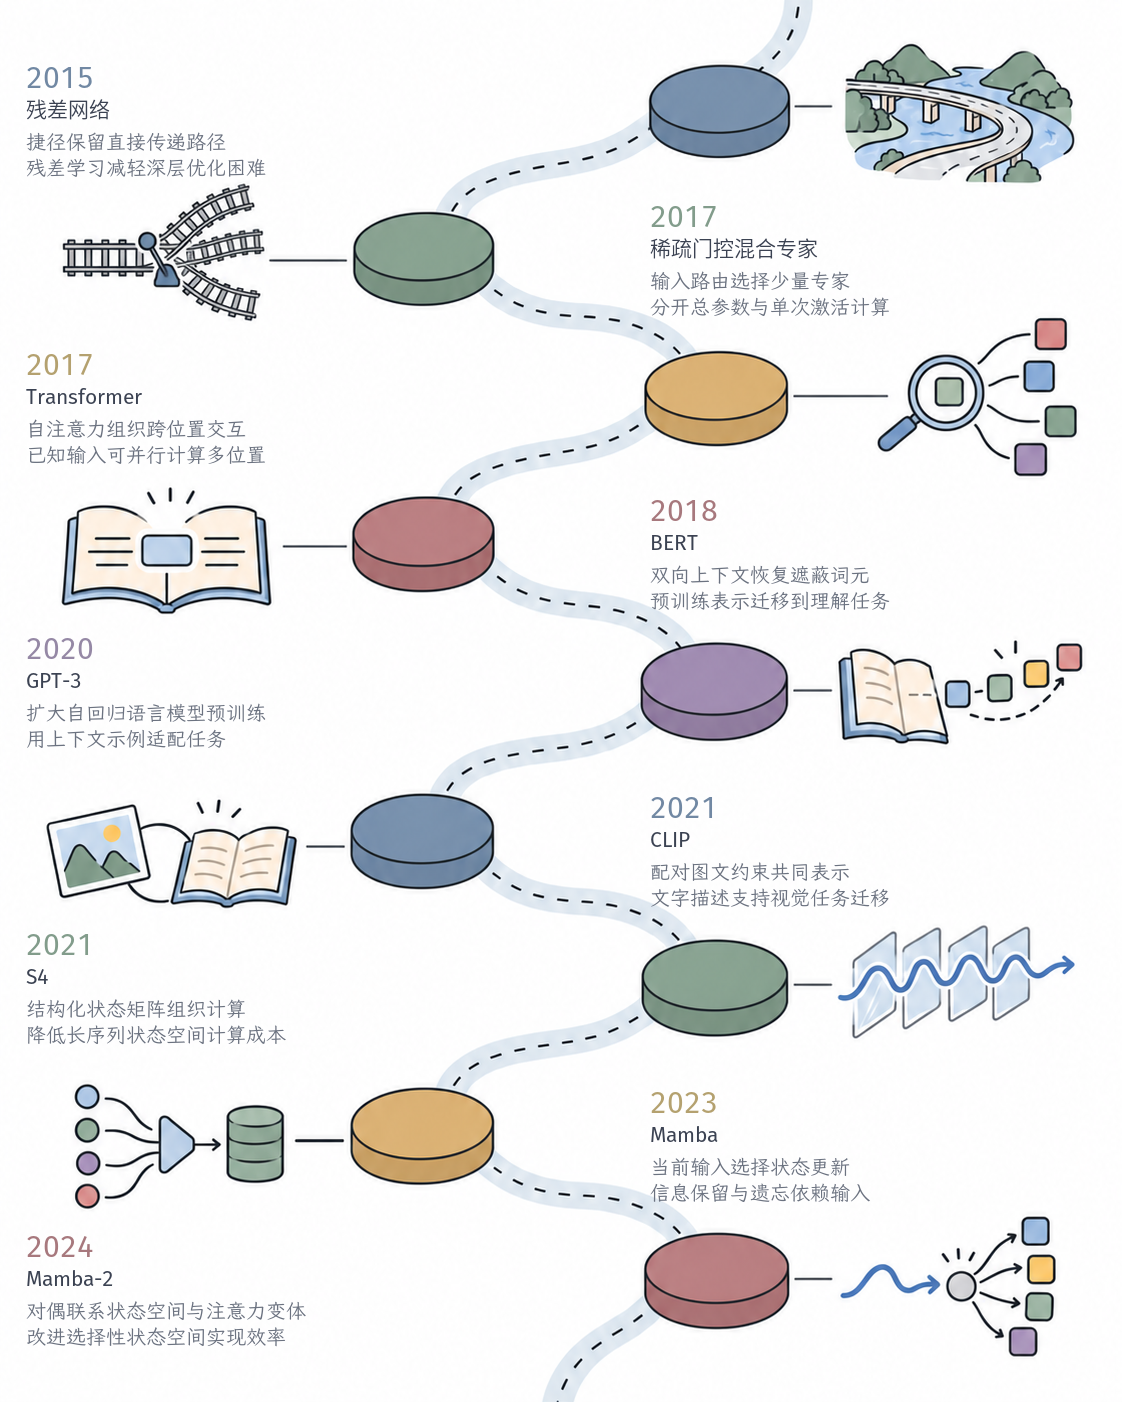
\includegraphics[width=149mm]{figures/05-neural-network-models/00-shared/generated/neural-network-history-recent/figure.png}
  \caption{神经网络发展的代表工作（2015—2024），承接图\ref{fig:neural-network-history}。各节点分别改变深层路径、内容读取、训练信息或资源组织，相应机制可以组合使用。读法和日期口径与前图相同。}
  \label{fig:neural-network-history-recent}
\end{figure*}

\subsection{面向能力、成本与可靠性的探索}
\label{sec:neural-history-current}

监督学习依赖大量人工标签，而现实中绝大多数观测没有标签，却并非不含信息。\term{自监督学习}（self-supervised learning）从数据本身构造训练目标：把输入的一部分遮住或挪走，让模型利用剩余部分预测被隐藏的内容，这样无须人工标注，原始记录自身就提供了答案。\term{预训练}（pre-training）是与之配合的训练安排：先在大规模数据上学习通用参数或表示，再把这些参数用于具体任务；它本身不指定目标，自监督、监督都可用于预训练。代表性工作中，BERT利用一个词左右两侧的上下文恢复被遮住的文本单位，GPT系列则按已有前缀逐步预测后续文本；GPT-3还研究了在不更新参数的情况下，用当前输入里给出的任务示例引导模型处理新任务的用法\scite{devlin2019,brown2020}。当信息来自不止一种模态时，\term{多模态学习}（multimodal learning）联合利用如图像与文本等不同类型的数据，CLIP用大量配对的图文学习把两者映射到同一表示空间，使文字描述可以直接参与视觉任务的定义\scite{radford2021}。这些方法扩大了模型可利用的信息来源，但是否能迁移到新任务，仍取决于预训练数据的覆盖面与目标任务的差距。

规模扩大同时带来现实的计算与存储约束。2024年前后的代表性工作继续在“能力—成本”之间寻找空间：Mamba-2利用特定条件下状态空间模型与一类注意力计算之间的数学联系改进计算组织；DeepSeek-V3继续研究稀疏专家架构下的训练与执行安排\scite{dao2024mamba2,deepseek2024v3}。增加总参数量、减少单次激活的专家数、压缩需要保存的历史状态，针对的是不同的资源账单：状态压缩可能丢掉任务真正需要的远期信息，稀疏专家仍需在设备间路由和汇集结果，因此任何效率结论都要结合任务规模与硬件实现评价，不能只比较参数总数。

最后，能力评价正在与可靠性评价分开。基准测试上的高正确率，并不能单独回答这些同样重要的问题：模型给出的概率是否可信地反映不确定性？换到来源不同的数据上是否仍然有效？生成的陈述是否符合事实？改进手段也应区分两类：后训练通过进一步学习实际改变模型参数（如针对人类偏好的调整）；推理阶段的技术则不改动参数，而是在本次预测中增加候选生成、搜索或验证步骤。两者都可能提高某项指标，也都带来额外计算成本。面对任何新工作，只有先明确它的任务定义、数据范围和检验对象，才能判断它究竟移除了哪个环节的障碍。

\FloatBarrier

\section{本章小结}
\label{sec:neural-overview-summary}

本章围绕“神经网络比传统线性模型多了什么”展开。核心答案是：神经网络把\emph{表示变换}纳入学习范围——隐藏层在任务损失的引导下改造输入坐标，使后续层在更友好的表示上完成预测；非线性激活是多层网络区别于单层线性模型的关键，没有它，任意多层线性变换都会合并成一次线性变换。同层内多个单元分布式地共同表示信息，不同层之间层次化地逐级组合更复杂的特征；网络结构则通过局部连接、参数共享、隐状态等设计注入归纳偏置，在利用数据规律的同时也限定了可表达的函数。表示能力、优化和泛化是三个必须分开评价的问题。

人工神经网络从生物神经系统借用了名称和功能直觉：人工单元对应“多输入整合后决定输出”，但舍去了脉冲时序、化学突触和动态膜电位；结构上的局部处理与层次组合受视觉系统启发，学习规则上则与赫布可塑性等局部机制分道扬镳，标准反向传播依据的是整体任务损失。判断一个网络应分别考察三个相互独立的维度：层间连接是否有回返（前馈还是循环）、信息按什么范围和权重交互（全连接、卷积、消息传递、注意力）、信号用连续值还是脉冲事件编码；这些描述可以自由交叉。

历史回顾则显示，这个领域围绕相继出现的障碍推进：阈值单元回答“网络能计算什么”，感知机把权重变为可学习，异或批评暴露了单层局限，反向传播解决了隐藏层的信用分配，卷积、LSTM、残差连接等结构分别利用了图像、序列和深度上的规律，注意力、专家路由和状态空间模型让计算随内容或历史组织，自监督预训练与多模态学习扩展了训练信息的来源，而成本与可靠性成为当前与能力并列的评价对象。后续章节将依次介绍前馈、卷积、循环、图、注意力与脉冲等具体架构，以及训练与泛化的系统方法；读者可以带着“它改变了三个问题中的哪一个”这一视角进入后续内容。

\paragraph{扩展阅读}
Goodfellow等的《深度学习》系统介绍表示、优化与统计学习，Bishop与Bishop的教材进一步联系现代网络结构\scite{goodfellow2016,bishop2024deep}

\chapter{前馈神经网络}
\label{chap:feedforward-networks}

第~\ref{chap:neural-network-overview}章用异或说明了隐藏表示的作用：两个非线性单元就能把原始坐标中无法线性分开的样本变成可分的表示。但那组权重是手工给出的，真实数据有成千上万个参数，不可能手工填写。本章要把这个演示变成一套可以实际运行的方法，需要依次回答三个问题：网络内部的计算究竟怎样组织（结构问题）？这些参数怎样从数据中自动得到（学习问题）？又凭什么相信在训练数据上表现好的网络，对没见过的新样本仍然可靠（泛化问题）？

本章以最基础、也最常用的一类网络——层状、全连接的前馈神经网络——为对象，把前章的函数复合落实为可计算、可求导的具体模型。本章的推进路线是：先规定一次预测中数据如何逐层流动，以及不同任务末端应该输出什么、用什么损失打分（\ref{sec:ffn-structure}节）；再解决训练的两个前置环节——参数的初始取值和反向传播这一核心求导算法，并说明实际框架如何自动完成求导（\ref{sec:ffn-learning}节）；然后把模型接口扩展到设备型号、词这样的高维离散类别输入，即Embedding（\ref{sec:ffn-extensions}节）；最后从理论上严格区分三件容易混淆的事：网络\emph{能不能}表达目标函数、优化算法\emph{能不能}找到好参数、找到的参数在新数据上\emph{风险有多大}（\ref{sec:ffn-theory}节）。阅读本章需要用到向量与矩阵运算、偏导数与链式法则，以及前几卷的损失、梯度下降等概念。

\section{网络结构}
\label{sec:ffn-structure}

本节先把“一个网络”精确地写成可以逐行实现的计算。所谓\emph{前馈}，规定的只是计算依赖的方向：同一次前向计算中，信息从输入出发逐层流向输出，后面的结果不会通过任何有向环再流回上游去影响本次计算。至于每层内部具体如何连接、一层放多少个单元，则是可以另行选择的设计。我们采用最简单也最稠密的一种安排——全连接的逐层结构，并把一次预测拆成三个环节反复观察：先对输入做\emph{加权组合}，再作\emph{非线性响应}形成新特征，最后由一个与任务相配的\emph{输出层}给出预测。

\subsection{神经元}
\label{sec:ffn-neuron}

网络的最小构件是一个人工神经元。它做的事可以用一句话概括：读取若干个数值，判断这些数值整体上支持还是反对它所关注的某种模式，再给出一个响应强度。这种“判断”不是硬规则，而是通过加权求和实现的。设单元的输入为$\bm{u}\in\mathbb{R}^{m}$，权重为$\bm{w}\in\mathbb{R}^{m}$，偏置为$b\in\mathbb{R}$，则
\begin{equation}
  z=\bm{w}^{\top}\bm{u}+b,
  \qquad h=\sigma(z)\text{。}
  \label{eq:ffn-unit}
\end{equation}
先看加权和$z=\bm{w}^{\top}\bm{u}+b$。内积$\bm{w}^{\top}\bm{u}$可以从几何上理解：当$\bm{u}$与权重向量$\bm{w}$方向接近时内积较大、方向相反时较小甚至为负，因此权重$\bm{w}$相当于刻划了单元“期待看到的输入方向”——输入越符合这个方向，加权和越高。每个权重决定对应输入以多大强度、正向还是负向影响结果。偏置$b$则是在不看任何输入时就存在的一个基准分，它改变单元开始响应的位置：没有偏置时，ReLU单元正负区域的分界线$\bm{w}^{\top}\bm{u}=0$被迫经过原点；加入偏置后这条分界可以平移到任意位置，单元的判定因此不再受“原点必须在边界上”的限制。

加权和之后还要经过激活函数$\sigma$。这里的$z$称为\term{预激活值}（pre-activation），即非线性变换之前的原始加权结果；$h$是非线性变换后的单元输出。为什么不能直接输出$z$？因为如果每个单元都只做加权求和，上一章已经证明，多层堆叠仍会合并成一次线性变换；正是$\sigma$的非线性让多层网络有了超出线性模型的能力，各种$\sigma$的选择见\ref{sec:ffn-activations}节。

单个单元只能产生一个新特征。让许多个这样的单元并排，各自用不同的权重读取同一组输入，就能同时产生一组不同视角的新坐标，这就是\term{全连接层}（fully connected layer）：下一层的每个单元都与上一层的每个单元相连。把一个单元的权重作为矩阵的一行，整层计算就可以用一次矩阵乘法完成，而不必逐个单元循环。沿用前章的列向量约定，设网络有$L$个隐藏层，输入为$\bm{x}\in\mathbb{R}^{d}$，令$d_0=d$、$\bm{h}^{(0)}=\bm{x}$，各隐藏层依次计算
\begin{equation}
  \begin{aligned}
    \bm{z}^{(\ell)}
      &=\bm{W}_\ell\bm{h}^{(\ell-1)}+\bm{b}_\ell,\\
    \bm{h}^{(\ell)}&=\sigma_\ell\!\left(\bm{z}^{(\ell)}\right),
    \qquad \ell=1,\ldots,L\text{。}
  \end{aligned}
  \label{eq:ffn-hidden-layers}
\end{equation}
其中$\bm{W}_\ell\in\mathbb{R}^{d_\ell\times d_{\ell-1}}$、$\bm{b}_\ell\in\mathbb{R}^{d_\ell}$，$\bm{z}^{(\ell)}$和$\bm{h}^{(\ell)}$都属于$\mathbb{R}^{d_\ell}$，$\sigma_\ell$逐坐标作用。上标$\ell$表示层的位置，不是幂，也不是参数更新的迭代步。

隐藏层之后还需一个与任务相配的输出层。记原始输出为$\bm{a}\in\mathbb{R}^{q}$、$d_{L+1}=q$，完整模型写为
\begin{equation}
  \begin{aligned}
    \bm{a}&=\bm{W}_{L+1}\bm{h}^{(L)}+\bm{b}_{L+1},\\
    \widehat{\bm{y}}&=g(\bm{a})\text{。}
  \end{aligned}
  \label{eq:ffn-output-map}
\end{equation}
矩阵$\bm{W}_{L+1}\in\mathbb{R}^{q\times d_L}$和向量$\bm{b}_{L+1}\in\mathbb{R}^{q}$参与学习，输出变换$g$由任务决定。$g$可以是恒等映射，也可以把得分转换为概率。用$\bm{\theta}\in\mathbb{R}^{p}$收集全部权重与偏置，模型记为$\bm{f}_{\bm{\theta}}(\bm{x})=\widehat{\bm{y}}$；标量输出时写$f_{\bm{\theta}}$。

图~\ref{fig:ffn-architecture}展示了这种分层依赖。输入层只提供数据，不计算一组新的可学习参数；隐藏层的每个坐标都是一次式\eqref{eq:ffn-unit}的计算。这就是前章引入的多层感知机：具有一个或多个全连接隐藏层、用非线性变换构造表示的前馈网络。这里的MLP采用可供梯度计算的非线性激活，区别于早期感知机作硬判定的阈值响应。

\begin{figure*}[htb]
  \centering
  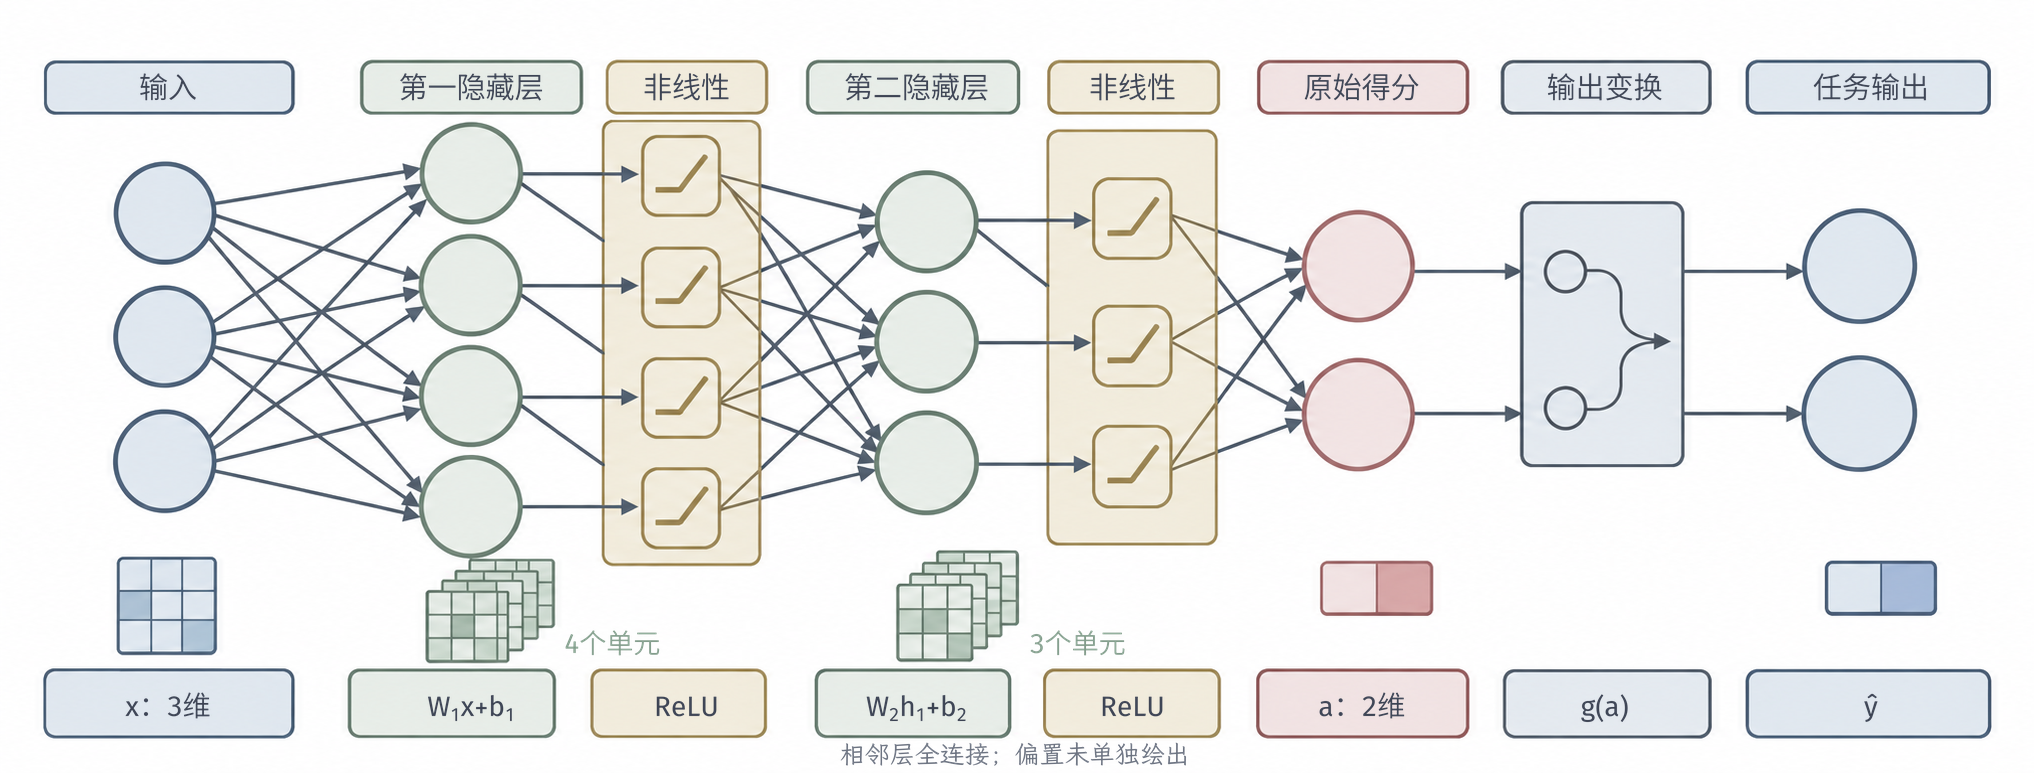
\includegraphics[width=169.000mm]{figures/05-neural-network-models/00-shared/generated/ffn-architecture/figure.png}
  \caption{两个隐藏层的全连接前馈网络。左侧单元提供输入$\bm{x}$，中间两层计算隐藏表示，右侧单元产生原始得分$\bm{a}$，之后再使用任务规定的输出变换$g$。细线表示可学习的连接，层间箭头标明前向计算方向；每个目标单元还具有一个未画出的偏置。图中层宽依次为$3,4,3,2$，只是结构示例。}
  \label{fig:ffn-architecture}
\end{figure*}

对没有参数共享的上述网络，参数总数为
\begin{equation}
  p=\sum_{\ell=1}^{L+1}d_\ell(d_{\ell-1}+1)\text{。}
  \label{eq:ffn-parameter-count}
\end{equation}
这个式子可以这样核对：第$\ell$层有$d_\ell$个单元，每个单元读取前一层$d_{\ell-1}$个输出，需要$d_{\ell-1}$个输入权重，再加上$1$个偏置，于是每个单元有$d_{\ell-1}+1$个参数，整层为$d_\ell(d_{\ell-1}+1)$，各层相加即为总数。若输入维度为$100$，两个隐藏层宽度均为$64$，输出维度为$1$，参数量为$64\times101+64\times65+65=10689$。这个数字主要被$100\times64$的第一层占据，说明输入编码的维度和层宽会直接决定模型规模；这也是为什么面对高维输入（如图像的几十万像素），后面章节会用卷积等结构来避免全连接带来的参数爆炸。忽略激活和偏置的较小开销，一次单样本前向计算的乘加量与$\sum_\ell d_\ell d_{\ell-1}$同阶，因为计算量主要花在每层的矩阵乘法上。需要提醒的是，参数量和计算量只描述\emph{规模}：同样数量的参数能表达哪些关系由连接方式与激活函数决定，而预测是否可靠还需要训练数据与泛化分析来回答。

本文把$L$称为隐藏层数，把$d_\ell$称为第$\ell$层宽度。文献中的\term{深度}（depth）有时包含输出层，有时只计隐藏层，两种计数相差一个输出层，因此深度比较需要采用同一口径。跨层连接只要不构成有向环，也可以保持前馈性质；本章的逐层推导采用普通串联结构。

\subsection{激活函数}
\label{sec:ffn-activations}

上一章已经证明，连续叠加仿射层仍然只是一次仿射变换，因此隐藏层必须使用非线性激活。但“非线性”只是一个最低要求，实践中激活函数的种类很多，初学时容易被一长串名字淹没。理解它们的关键是抓住一个统一的视角：\emph{激活函数决定一个预激活值$z$如何变成单元输出，而不同的“形状”会在三个方面产生不同后果}——它能表达什么样的输入—输出关系、反向传播时梯度能否顺利通过、输出落在什么数值范围。

为了让下面的介绍有线索可循，可以先按“形状”把常见函数分成几类。最朴素的基准是恒等函数（什么都不做）和阶跃函数（只给0/1硬判定）。在需要概率等有界输出时，会用到把任意实数压进有限区间的\emph{双侧饱和函数}，如Sigmoid和Tanh；它们在输入很大或很小时输出几乎不再变化，这种“压平”会带来梯度变小的问题。为缓解这一问题，\emph{整流函数}（以ReLU为代表）选择只截断负值、对正值原样放行，由此衍生出一批带泄漏、带上界的变体；\emph{指数型函数}让负值平滑地趋向一个有限下界而非硬截断；\emph{自门控函数}（Swish、GELU等）则让输入乘以一个随自身连续变化的“保留比例”，在正负区域之间平滑过渡。最后，Maxout和Softmax比较特殊：它们不逐个坐标独立作用，而是\emph{联合处理一组}预激活值。

需要事先说明三点阅读约定。其一，带可学习参数的函数（如PReLU、Swish）曲线形状会随训练改变，图中画出的具体参数值只是比较时的一个条件，不是固定结论。其二，随机型函数（如RReLU）在训练和预测两个阶段采用的规则可能不同。其三，除特别说明外，下面都把输入记为标量$z$、输出记为$\sigma(z)$，因为绝大多数激活是逐坐标独立作用的；理解了一个坐标上的形状，整层只是把同样的规则并行施加到每个坐标。

\subsubsection{恒等与阶跃}
\label{sec:ffn-activation-baselines}

若需要保留任意实数输出，可以使用\term{恒等函数}（identity function）；若只需要一个硬的二值判定，可以使用\term{阶跃函数}（step function）。两者分别为
\begin{equation}
  \operatorname{Identity}(z)=z,
  \qquad
  H(z)=\begin{cases}0,&z<0,\\1,&z\geq0\text{。}\end{cases}
  \label{eq:ffn-identity-step}
\end{equation}
恒等函数的导数为$1$，常用于回归输出或无需额外激活的投影；全部隐藏层都用恒等函数时，多层串联仍是仿射映射。阶跃函数适合表达阈值决策，但除阈值处不可微之外，在其余位置导数都为$0$，普通反向传播无法据此学习阈值单元的输入参数。预测时作硬判定与训练时使用连续可导替代，是两种不同用途。

\begin{figure*}[htb]
  \centering
  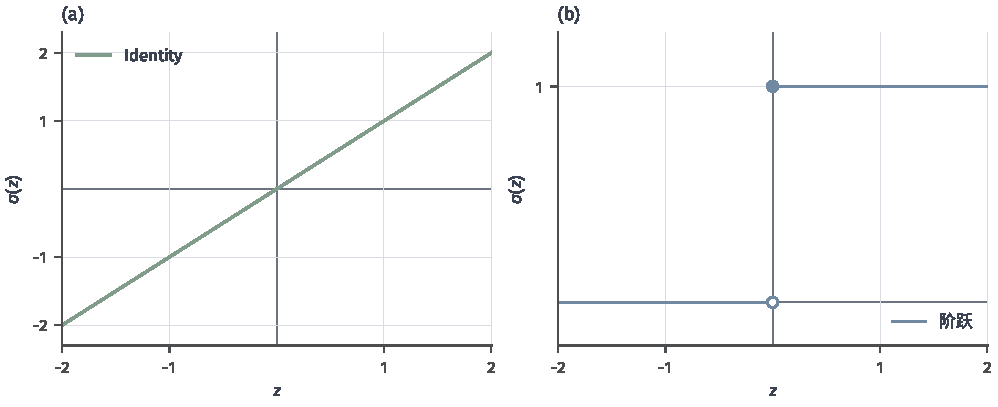
\includegraphics[width=159.059mm]{figures/05-neural-network-models/00-shared/matplotlib/ffn-activation-basics/figure.pdf}
  \caption{恒等函数与阶跃函数的比较。左图保留输入，斜率恒为$1$；右图按零阈值输出$0$或$1$，空心点和实心点区分$z=0$两侧的端点约定。横轴为预激活值$z$，纵轴为输出；阶跃图中的跳跃不能通过普通局部导数传递学习信号。}
  \label{fig:ffn-activation-basics}
\end{figure*}

\subsubsection{双侧饱和函数}
\label{sec:ffn-activation-saturating}

当一个单元需要产生概率、控制系数或有界状态时，把任意实数压到有限区间是直接的选择。\term{Logistic函数}产生$(0,1)$内的响应，实践中常直接称为Sigmoid；\term{双曲正切函数}（hyperbolic tangent, Tanh）产生$(-1,1)$内的响应。Sigmoid也可泛指具有S形曲线的一类函数，这里用$s$专门表示Logistic函数：
\begin{equation}
  \begin{aligned}
    s(z)&=\frac{1}{1+\exp(-z)},
    &s'(z)&=s(z)(1-s(z)),\\
    \tanh(z)&=\frac{\exp(z)-\exp(-z)}{\exp(z)+\exp(-z)},
    &\tanh'(z)&=1-\tanh^2(z)\text{。}
  \end{aligned}
  \label{eq:ffn-saturating-activations}
\end{equation}
当$|z|$很大时，输出接近两端的极限，导数趋近于零。这种\term{饱和}（saturation）意味着输入继续变化，输出却几乎不变。Sigmoid导数至多为$1/4$；Tanh在原点的导数为$1$，并满足$\tanh(z)=2s(2z)-1$。Tanh关于原点对称，可以产生正负响应，但只有对称输入分布等条件才能进一步推出输出均值为零。

Sigmoid适合二分类概率、多标签概率和取值在$(0,1)$的控制门。当损失与事件标签构成概率模型时，这一响应才作为相应事件的概率；用在隐藏层时，它只是有界特征值。Tanh适合需要正负有界状态的模块，例如后续循环网络中的候选状态。两者用于许多层连续串联时，饱和区的小导数可能参与梯度衰减；传播中的权重矩阵同时可以放大或缩小信号，完整梯度尺度由沿途的两种作用共同决定。

若希望避免指数运算，可以用分段线性函数近似上述有界响应。\term{硬Sigmoid}（hard sigmoid，也称Hard-Logistic）和\term{硬Tanh}（hard tanh）将线性段之外的值截到边界：
\begin{equation}
  \begin{aligned}
    \operatorname{HardSigmoid}(z)
      &=\min\{1,\max\{0,\tfrac14z+\tfrac12\}\},\\
    \operatorname{HardTanh}(z)&=\min\{1,\max\{-1,z\}\}\text{。}
  \end{aligned}
  \label{eq:ffn-hard-saturating-activations}
\end{equation}
本节的HardSigmoid在$(-2,2)$内斜率为$1/4$，区间外为$0$；HardTanh在$(-1,1)$内斜率为$1$，区间外为$0$，其负端输出是$-1$。分段边界处的导数需要约定。HardSigmoid的线性段并没有唯一标准，一些实现采用$z/6+1/2$并在$\pm3$处截断；不同斜率与截断点会改变响应及导数，移植模型需要采用与原实现相同的定义\scite{pytorchHardsigmoid}

两种硬近似可用于受计算资源限制的门控或范围约束，代价是拐点不可微，截断区内还会出现严格为零的梯度。\term{Softsign函数}提供另一种有界响应，用绝对值而非指数控制幅度：
\begin{equation}
  \operatorname{Softsign}(z)=\frac{z}{1+|z|},
  \qquad
  \operatorname{Softsign}'(z)=\frac{1}{(1+|z|)^2}\text{。}
  \label{eq:ffn-softsign}
\end{equation}
它的值域也是$(-1,1)$，一阶导数连续，尾部导数以多项式速度趋零。它可用于需要有界正负响应的隐藏层或状态映射；与Tanh相比，它的尾部导数衰减更慢，具体输入处的梯度大小仍由各自导数值决定。

\begin{figure*}[htb]
  \centering
  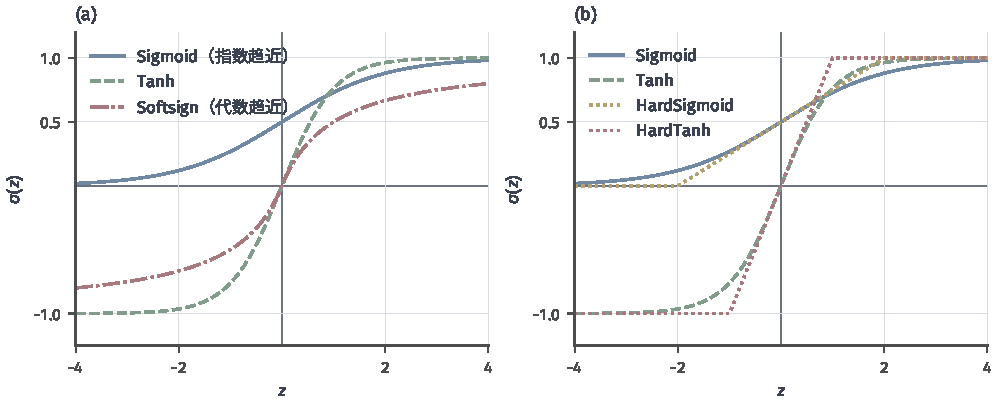
\includegraphics[width=159.059mm]{figures/05-neural-network-models/00-shared/matplotlib/ffn-activations/figure.pdf}
  \caption{双侧饱和激活函数。左图比较Logistic／Sigmoid、Tanh与Softsign；Softsign采用长虚线，以便在黑白打印中仍能与Sigmoid区分，图例同时指出前者按代数速度、后者按指数速度趋近渐近值。右图将HardSigmoid和HardTanh与对应平滑函数比较。HardSigmoid采用式\eqref{eq:ffn-hard-saturating-activations}中的斜率$1/4$及截断点$\pm2$。}
  \label{fig:ffn-activations}
\end{figure*}

\subsubsection{整流函数及其变体}
\label{sec:ffn-activation-rectifiers}

ReLU采用前章的$\rho(z)=\max\{0,z\}$，正半轴斜率为$1$，负半轴输出和导数都为$0$。它只需一次比较和一次取值，不涉及指数运算，并且能够产生严格为零的激活（即一批单元在某个样本上完全关闭），因而是全连接或卷积隐藏层最常用的基础选择。

ReLU的简洁也带来一个特有的训练现象。设想某个单元：对当前所有训练样本，它的加权和$z$都落在负半轴，于是输出恒为$0$。由于负半轴导数为$0$，损失对这个单元输入权重的梯度也是$0$，梯度下降不会再修改这些权重；权重不变，$z$的分布也不变，该单元就可能一直停在关闭状态，称为“单元失活”或“死亡ReLU”。需要澄清两点：失活是\emph{当前参数与当前数据共同}造成的结果，并非单元本身损坏；它也未必永久。如果更上游的表示在后续训练中发生变化，使某些样本的$z$回到正半轴，这个单元仍可能被重新激活。尽管如此，大面积失活意味着一部分参数事实上退出了学习，这正是后面引入“负半轴保留斜率”等变体的直接原因。

让负半轴保留非零斜率，可以避免该区域完全阻断局部梯度。\term{带泄漏的ReLU}（leaky ReLU）使用固定$0<\alpha<1$，\term{参数化ReLU}（parametric ReLU, PReLU）则把负半轴斜率作为待学习参数：
\begin{equation}
  \begin{aligned}
    \operatorname{LeakyReLU}(z)
      &=\max\{0,z\}+\alpha\min\{0,z\},\\
    \operatorname{PReLU}_j(z)
      &=\max\{0,z\}+\alpha_j\min\{0,z\}\text{。}
  \end{aligned}
  \label{eq:ffn-leaky-prelu}
\end{equation}
PReLU的$\alpha_j$可以按单元、通道设置，也可以在一层内共享；若不另加约束，它并不天然位于$(0,1)$。给定上游梯度，斜率参数的局部求导规则是$\partial\operatorname{PReLU}_j(z)/\partial\alpha_j=\min\{0,z\}$，共享斜率时要累加各使用位置的贡献。PReLU增加的参数量取决于共享方式，通常每个单元、通道或层只增加一个斜率参数\scite{he2015rectifiers}

Leaky ReLU适合希望保留负响应且不增加待学习参数的隐藏层，PReLU适合允许数据调整负响应强度的模块。\term{随机化带泄漏ReLU}（randomized leaky ReLU, RReLU）沿用同一分段形式，但训练时从预先规定的区间$[l,u]$均匀采样负斜率$\alpha$，其中$0<l<u<1$，预测时通常采用$(l+u)/2$。每次采样产生一条不同曲线，使同一负输入在训练中受到不同缩放。预测采用确定斜率；这种训练扰动对误差的作用需要在相应任务上评价\scite{xu2015rectified}

如果部署还要求限制正响应，可以使用\term{ReLU6函数}，即
\begin{equation}
  \operatorname{ReLU6}(z)=\min\{6,\max\{0,z\}\}\text{。}
  \label{eq:ffn-relu6}
\end{equation}
它在$(0,6)$内保留斜率$1$，在两侧导数为$0$，常与移动端模型及有限数值范围的设计联系在一起。MobileNetV2使用了这类有界整流响应，但其线性瓶颈层还刻意省略非线性，说明激活要按层的职责选择\scite{sandler2018mobilenetv2}相对于ReLU，新增上界让较大的正输入也进入零导数区，有限范围与梯度传递因此形成取舍。

\begin{figure*}[htb]
  \centering
  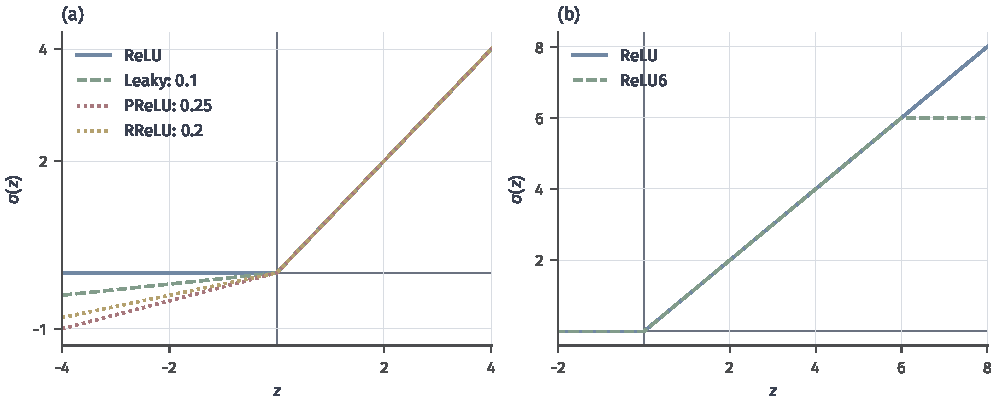
\includegraphics[width=159.059mm]{figures/05-neural-network-models/00-shared/matplotlib/ffn-activation-rectifiers/figure.pdf}
  \caption{整流函数与负斜率变体。左图固定Leaky ReLU的$\alpha=0.1$、PReLU的$\alpha_j=0.25$，并以$\alpha=0.2$画出RReLU训练阶段的一种可能曲线；三者的形状差异来自斜率选择，PReLU与RReLU的区别主要在参数取得方式。右图比较ReLU与ReLU6，展示$z>6$时的截断。两图横轴范围不同。}
  \label{fig:ffn-activation-rectifiers}
\end{figure*}

有界函数与整流函数的差异集中在表~\ref{tab:ffn-activation-bounded}中。Sigmoid、Tanh和Softsign限制两端幅度，ReLU只截断负半轴，ReLU6还限制正端；这种范围差异会直接改变哪些输入能够传递梯度。

\begin{table*}[htb]
  \centering
  \small
  \begin{tabularx}{\linewidth}{@{}l l X X@{}}
    \toprule
    函数 & 输出范围 & 导数与参数特点 & 适用场景及主要边界 \\
    \midrule
    Identity & $\mathbb{R}$ & 导数为$1$ & 回归输出、线性投影；不增加非线性 \\
    阶跃 & $\{0,1\}$ & 非阈值处导数为$0$ & 硬判定；不能直接靠普通反向传播训练 \\
    Sigmoid & $(0,1)$ & 两端导数趋零 & 二分类、多标签、控制门 \\
    Tanh & $(-1,1)$ & 两端导数趋零 & 有界正负状态；深层饱和需关注 \\
    HardSigmoid & $[0,1]$ & 截断区导数为$0$ & 简单门控；需核对斜率与截断点 \\
    HardTanh & $[-1,1]$ & 截断区导数为$0$ & 有界状态；拐点与严格零梯度 \\
    Softsign & $(-1,1)$ & 一阶连续，尾部导数趋零 & 有界正负表示；尾部衰减方式不同 \\
    ReLU & $[0,+\infty)$ & 负半轴为$0$，正半轴为$1$ & 全连接、卷积隐藏层；可能失活 \\
    Leaky ReLU & $\mathbb{R}$ & 固定正负斜率 & 保留负梯度；斜率需设定 \\
    PReLU & 依赖$\alpha_j$ & 负斜率参与学习 & 学习响应形状；需说明参数共享方式 \\
    RReLU & $\mathbb{R}$ & 训练时随机负斜率 & 隐藏层训练扰动；预测规则不同 \\
    ReLU6 & $[0,6]$ & 两侧截断，中间斜率为$1$ & 有限范围、移动端；正端也会饱和 \\
    \bottomrule
  \end{tabularx}
  \caption{有界响应与整流激活的比较。Leaky ReLU和RReLU的范围按正负斜率均为正且非零书写；PReLU若不限制斜率，其输出范围随参数改变。所有分段函数都需在不可微边界约定求导规则。}
  \label{tab:ffn-activation-bounded}
\end{table*}

即使都用于限制输出幅度，求导行为也可能不同。Tanh和HardTanh都提供有界正负响应；按解析定义，前者在有限输入下保留非零导数，后者在截断区的导数严格为零。选择范围约束时，还需判断训练中的预激活值是否经常落到这些区域。

\subsubsection{指数型与平滑整流函数}
\label{sec:ffn-activation-exponential}

固定负斜率让负输出无限下降，另一种做法是使负响应逐渐接近一个有限下界。\term{指数线性单元}（exponential linear unit, ELU）在正半轴保留输入，在负半轴使用指数曲线：
\begin{equation}
  \operatorname{ELU}_{\alpha}(z)=
  \begin{cases}
    z,&z>0,\\
    \alpha(\exp(z)-1),&z\leq0,
  \end{cases}
  \qquad \alpha>0\text{。}
  \label{eq:ffn-elu}
\end{equation}
负半轴导数为$\alpha\exp(z)$，对有限负输入非零，但在$z\to-\infty$时趋零；输出趋近$-\alpha$。ELU连续，只有$\alpha=1$时左右一阶导数才在原点一致，但原点左右的二阶导数不同。ELU可用于希望保留负值并控制负端幅度的隐藏层；负响应允许层输出向两侧分布，实际均值仍由输入分布和权重决定\scite{clevert2016elu}

仅知道单个单元怎样响应，还不足以判断多层堆叠后会发生什么，这里引入一个新的视角。固定网络参数，让输入随样本变化，则每个单元的输出都是一个随机变量：可以用均值描述它的“中心位置”、用方差描述它的“波动幅度”。当信号一层层传下去时，这两个统计量会被每层的权重和激活不断改变。如果每经过一层方差就放大一些，深层的输入数值会越来越大；如果方差不断缩小，数值又会被压向零。这两种趋势累积几十层后，都会让训练变得困难——前者容易使数值溢出或梯度过大，后者则使不同输入难以区分、梯度微弱。因此，一个自然的设计目标是：让每层输出的均值大致保持在零附近、方差大致保持在一附近，使信号在层间传播时尺度稳定。SELU正是为这一目标设计的激活函数。

\term{缩放指数线性单元}（scaled exponential linear unit, SELU）在ELU的基础上整体乘一个固定系数$\kappa$：
\begin{equation}
  \operatorname{SELU}(z)=\kappa
  \begin{cases}
    z,&z>0,\\
    \alpha(\exp(z)-1),&z\leq0,
  \end{cases}
  \label{eq:ffn-selu}
\end{equation}
其中常用常数为$\alpha\approx1.6733$、$\kappa\approx1.0507$。它用于\term{自归一化网络}（self-normalizing neural network），即在规定假设下让层间激活的均值与方差趋向受控范围的前馈网络。相应分析依赖输入与权重的统计条件；常配合输入标准化、权重方差为$1/\mathrm{fan\text{-}in}$的初始化，以及为保持统计量设计的AlphaDropout。这里fan-in是一个单元的输入连接数，初始化的具体说明见第~\ref{sec:ffn-initialization}节。自归一化结论依赖这套激活、初始化与丢弃规则共同满足统计假设，替换其中一项也会改变分析条件\scite{klambauer2017selu}

具体地，把一层输出的均值、方差记为$(\mu,\nu)$，下一层对应统计量记为$(\widetilde\mu,\widetilde\nu)$。原分析在输入坐标独立且同均值、同方差的设定下采用加权和的正态近似，这项近似本身也是后续结论的条件。当单元权重的和为零、平方和为一且偏置为零时，SELU中$\alpha$与$\kappa$的理论取值按统计映射把$(0,1)$仍送到$(0,1)$的要求选择。这就是零均值、单位方差的不动点含义。负端饱和与正端大于$1$的斜率分别提供限制幅度与放大响应的两种作用，常数选择让二者在统计目标附近形成平衡。在论文限定的输入统计量和权重范围内，偏离这一点的小扰动还会被后续映射缩小；训练中的任意权重和任意相关输入不自动满足这些条件。

训练时若要随机屏蔽活动值，还需避免屏蔽本身破坏上述统计目标。AlphaDropout（alpha dropout）把被屏蔽的值替换为SELU的负饱和值$\alpha_-=-\kappa\alpha$，再作仿射修正。以一个均值为零、方差为一的活动值$h$为例，令保留概率为$\pi\in(0,1]$，独立掩码$m_{\mathrm d}\sim\operatorname{Bernoulli}(\pi)$在保留时为$1$、替换时为$0$，替换后的值为
\[
  \widetilde h=m_{\mathrm d}h+(1-m_{\mathrm d})\alpha_-\text{。}
\]
保留部分的均值为零，替换部分恒为$\alpha_-$，所以$\mathbb E[\widetilde h]=(1-\pi)\alpha_-$。方差既包括保留时原有波动的贡献$\pi$，也包括保留与替换两种均值差异的贡献$\pi(1-\pi)\alpha_-^2$。因此可先减去新均值，再除以新标准差，得到
\[
  h_{\mathrm d}=
  \frac{\widetilde h-(1-\pi)\alpha_-}
       {\sqrt{\pi[1+(1-\pi)\alpha_-^2]}}\text{。}
\]
在上述均值、方差和掩码独立条件下，$h_{\mathrm d}$重新具有均值零与方差一。预测时关闭这项随机替换与配套修正，使用原有活动值。这个关系对活动值和掩码的分布计算，并不要求每个有限小批量的样本均值、样本方差都精确等于目标；它也没有单独保证整个训练过程收敛或预测风险降低。

如果目标是输出严格正值而又保持平滑，可以使用\term{Softplus函数}：
\begin{equation}
  \operatorname{Softplus}(z)=\log(1+\exp(z)),
  \qquad \operatorname{Softplus}'(z)=s(z)\text{。}
  \label{eq:ffn-softplus}
\end{equation}
它在正端接近$z$，在负端趋近$0$，但有限输入下输出严格大于$0$，不会产生ReLU式的精确零激活。Softplus可作为平滑隐藏激活，也适合将任意得分映射为正尺度、强度或方差参数；需要严格正下界时还可加上一个固定小常数。计算时使用$\max\{z,0\}+\log(1+\exp(-|z|))$可避免指数溢出。因此Softplus的用途由平滑性和正值约束决定；隐藏分类响应与正尺度输出采用它时，所要满足的条件不同。

\begin{figure}[htbp]
  \centering
  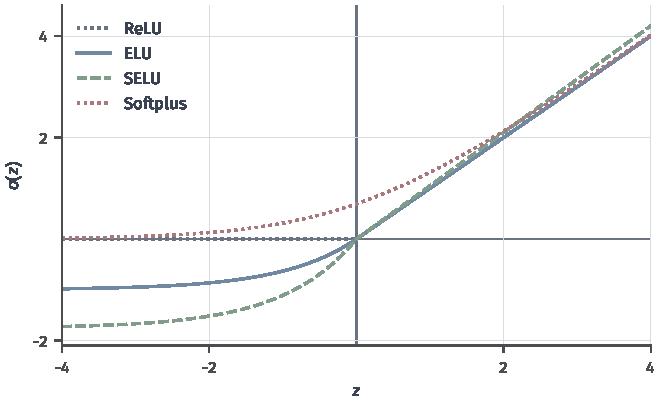
\includegraphics[width=105.412mm]{figures/05-neural-network-models/00-shared/matplotlib/ffn-activation-exponential/figure.pdf}
  \caption{ELU、SELU与Softplus的响应。ELU使用$\alpha=1$，SELU使用式\eqref{eq:ffn-selu}中的常数，ReLU作为共同参照。ELU与SELU允许负输出并在负端趋向有限下界；Softplus始终为正，且平滑地趋近正半轴上的线性响应。}
  \label{fig:ffn-activation-exponential}
\end{figure}

\subsubsection{自门控函数}
\label{sec:ffn-activation-self-gated}

ReLU根据输入的正负作硬切换，也可以让输入乘一个连续变化的系数。\term{Swish函数}使用输入自身计算保留系数：
\begin{equation}
  \operatorname{Swish}_{\beta}(z)=z s(\beta z),
  \qquad \beta\geq0\text{。}
  \label{eq:ffn-swish}
\end{equation}
$\beta$可以固定，也可以参与学习。$\beta=0$时函数为$z/2$；$\beta=1$时得到\term{Sigmoid加权线性单元}（sigmoid-weighted linear unit, SiLU）；当$\beta\to+\infty$时，对每个固定输入趋向ReLU。这里的极限只描述固定输入处的响应值；不同$\beta$还会改变各输入处的导数，从而改变训练过程\scite{ramachandran2017swish}

计算输入敏感度及可学习门参数的梯度，需要分别对输入与门参数求导：
\begin{equation}
  \begin{aligned}
    \operatorname{Swish}_{\beta}'(z)
      &=s(\beta z)+\beta z s(\beta z)(1-s(\beta z)),\\
    \frac{\partial\operatorname{Swish}_{\beta}(z)}{\partial\beta}
      &=z^2s(\beta z)(1-s(\beta z))\text{。}
  \end{aligned}
  \label{eq:ffn-swish-derivatives}
\end{equation}
SiLU采用上述Swish族中固定门参数的实例。SiLU在强化学习函数逼近等场景中也有使用\scite{elfwing2018silu}SiLU可作为全连接、卷积或门控前馈模块中的平滑激活；在有限负区间内导数可能为负，负尾部导数又趋零。若学习$\beta$并要求保持非负，还需明确约束方式。

\begin{figure}[htbp]
  \centering
  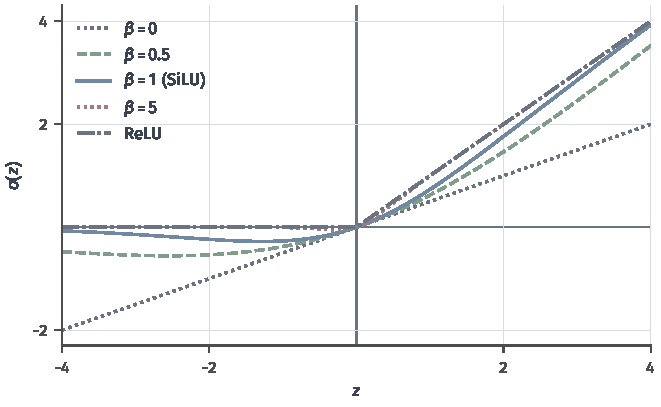
\includegraphics[width=105.412mm]{figures/05-neural-network-models/00-shared/matplotlib/ffn-activation-swish/figure.pdf}
  \caption{Swish在不同$\beta$下的函数图像。$\beta=0$给出线性函数$z/2$，$\beta=1$就是SiLU，较大的$\beta$逐渐形成接近ReLU的响应。图中参数固定为$0,0.5,1,5$，ReLU用作极限参照；它不展示可学习$\beta$在某次训练中的实际轨迹。}
  \label{fig:ffn-activation-swish}
\end{figure}

\term{高斯误差线性单元}（Gaussian error linear unit, GELU）采用标准正态累积分布函数$\Phi$作为保留系数：
\begin{equation}
  \operatorname{GELU}(z)=z\Phi(z),
  \qquad \operatorname{GELU}'(z)=\Phi(z)+z\varphi(z)\text{。}
  \label{eq:ffn-smooth-gates}
\end{equation}
其中$\varphi(z)=\exp(-z^2/2)/\sqrt{2\pi}$是标准正态密度。GELU在全实数上平滑，但公式中的分布函数为每个输入确定一个保留系数，执行时采用确定响应。它常作为Transformer前馈模块的激活选择，平滑性保证局部导数连续，训练所得解的损失仍由完整目标与更新过程决定。常见近似为$z s(1.702z)$，或者
\begin{equation}
  \operatorname{GELU}(z)\approx
  \frac z2\left(1+\tanh\!\left[\sqrt{\frac2\pi}
  (z+0.044715z^3)\right]\right)\text{。}
  \label{eq:ffn-gelu-approximation}
\end{equation}
使用哪种近似会改变实际数值与导数，这会影响复现结果，因此模型记录需要标明精确式或近似式；GELU与SiLU的保留系数不同\scite{hendrycks2016gelu}

保留系数的含义可以用几个输入看清。标准正态分布关于零对称，所以$\Phi(0)=1/2$；此时输入恰为零，GELU输出仍为零。取$z=1$和$z=-1$时，保留系数分别约为$0.8413$和$0.1587$，输出因而约为$0.8413$和$-0.1587$。较大的正输入对应接近一的系数，较大的负输入对应接近零的系数；负输入没有像ReLU那样一律被置零，而是随输入位置受到不同程度的缩放。

\term{Mish函数}进一步用Softplus和Tanh形成平滑的保留系数\scite{misra2019mish}其定义为
\begin{equation}
  \operatorname{Mish}(z)=z\tanh(\operatorname{Softplus}(z))\text{。}
  \label{eq:ffn-mish}
\end{equation}
令$t=\tanh(\operatorname{Softplus}(z))$，乘积与链式法则给出导数$t+zs(z)(1-t^2)$。Mish在负半轴保留一段负响应，负尾部趋近零，正端接近线性，可作为视觉网络或普通隐藏层的另一种平滑选择；原论文的比较是在指定模型与数据上进行的，这些设置决定了所报告收益的适用范围。

这些平滑函数需要指数、Tanh或正态分布函数计算。若希望用简单分段运算近似SiLU，可使用\term{硬Swish}（hard swish, Hardswish）。MobileNetV3在面向移动端的结构中使用这种响应\scite{howard2019mobilenetv3}其定义为
\begin{equation}
  \operatorname{Hardswish}(z)=z\frac{\operatorname{ReLU6}(z+3)}6
  =\begin{cases}
    0,&z\leq-3,\\
    z(z+3)/6,&-3<z<3,\\
    z,&z\geq3\text{。}
  \end{cases}
  \label{eq:ffn-hardswish}
\end{equation}
它在中间区间的导数为$(2z+3)/6$，在两端分别为$0$和$1$，在$\pm3$处不具有唯一导数。这里的门采用斜率$1/6$的硬Sigmoid形式，与前面斜率$1/4$的版本具有不同的线性段与截断点。实际速度取决于算子与硬件实现，而不只取决于公式中出现几个基本运算。

\begin{figure*}[htb]
  \centering
  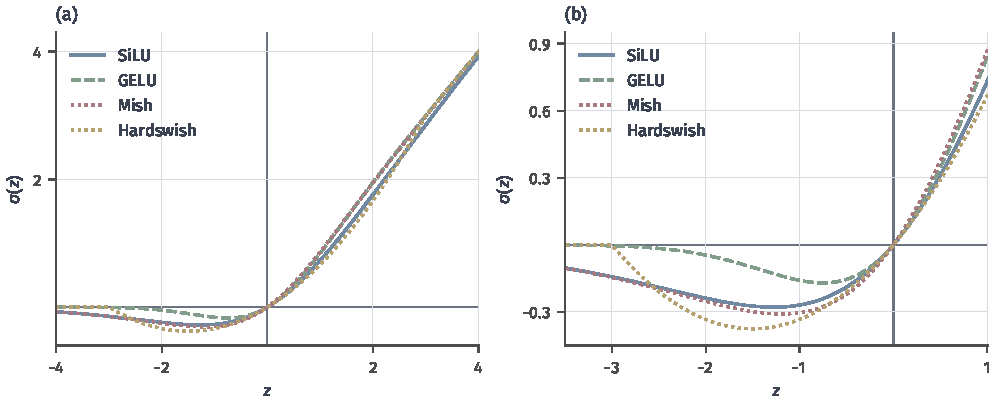
\includegraphics[width=159.059mm]{figures/05-neural-network-models/00-shared/matplotlib/ffn-activation-smooth/figure.pdf}
  \caption{SiLU、GELU、Mish与Hardswish。左图展示整体响应，右图放大原点附近的负值和过渡区域；GELU按标准正态累积分布函数计算响应。它们在正端接近线性，但负区间的形状和拐点不同。SiLU、GELU与Mish平滑，Hardswish含有分段边界；两图使用不同坐标范围以显示细节。}
  \label{fig:ffn-activation-smooth}
\end{figure*}

\subsubsection{Maxout与Softmax}
\label{sec:ffn-activation-vector}

以上函数分别作用于一个标量。若希望一个单元从若干候选响应中选择最大者，可以使用\term{Maxout单元}（maxout unit）：它先计算$K$个仿射响应，再取最大值，响应的分段形状由权重学习得到。对于输入$\bm{u}\in\mathbb{R}^{m}$，其定义为
\begin{equation}
  z_k=\bm{w}_k^{\top}\bm{u}+b_k,
  \qquad h=\max_{1\leq k\leq K}z_k\text{，}
  \label{eq:ffn-maxout}
\end{equation}
其中每个$\bm{w}_k\in\mathbb{R}^{m}$、$b_k\in\mathbb{R}$都参与学习。只有一个严格最大响应时，梯度传给这一响应；多个响应并列最大时需约定分配方式。固定一个响应为零、另一个为$\bm{w}^{\top}\bm{u}+b$，就得到ReLU这一特殊形式。一个Maxout单元对输入表示为凸分段仿射函数；多层复合还包含可正可负的线性组合，完整网络的凸性须由整体计算判断\scite{goodfellow2013maxout}

Maxout适合希望学习分段响应形状的隐藏单元，也曾与Dropout联合研究。相对于一个普通仿射响应，它有$K$套权重与偏置，参数和响应计算量通常约增至$K$倍，这$K$套响应都要分别计算。梯度的截断由最大值选择决定：长期未被选中的分支可能收不到梯度。它还不再是式\eqref{eq:ffn-hidden-layers}中逐坐标作用于一个仿射响应的激活，反向计算需使用最大值选择对应的规则。

把$K$个得分转换为互斥事件的概率时，可以用\term{归一化指数映射}（softmax）让较大得分对应较大概率，并把概率总和固定为一。
对$\bm{z}\in\mathbb{R}^{K}$，其第$k$个输出为
\begin{equation}
  p_k=\operatorname{softmax}(\bm{z})_k
  =\frac{\exp(z_k)}{\sum_{j=1}^{K}\exp(z_j)},
  \qquad \sum_{k=1}^{K}p_k=1\text{。}
  \label{eq:ffn-softmax-activation}
\end{equation}
每个概率依赖全部输入坐标；画一维响应曲线时，需要固定其余坐标。
Jacobian矩阵描述每项概率对各得分的变化：
$\partial p_k/\partial z_j=p_k(\mathbb I\{k=j\}-p_j)$。

这里的指示记号$\mathbb I\{k=j\}$在两个索引相等时取$1$，否则取$0$。固定输出索引$k$，当改变的输入也是$z_k$时，分子与分母都会变化；当改变的是另一个$z_j$时，只有共同分母变化。按商的求导规则，两种情况分别为
\[
  \begin{aligned}
    \frac{\partial p_k}{\partial z_k}
      &=\frac{\exp(z_k)\sum_{i=1}^{K}\exp(z_i)-\exp(2z_k)}
              {\left(\sum_{i=1}^{K}\exp(z_i)\right)^2}
        =p_k(1-p_k),\\
    \frac{\partial p_k}{\partial z_j}
      &=-\frac{\exp(z_k)\exp(z_j)}
              {\left(\sum_{i=1}^{K}\exp(z_i)\right)^2}
        =-p_kp_j,\qquad j\ne k\text{。}
  \end{aligned}
\]
两种结果合在一起，就是上面的指示记号形式；Jacobian矩阵的第$k$行、第$j$列记录的正是这一变化率。
提高本类得分会增大本类概率，提高另一类得分则经共同分母降低本类概率；
若固定一个输入得分$z_j$，再把所有输出坐标$k=1,\ldots,K$对它的导数相加，则
\[
  \sum_{k=1}^{K}\frac{\partial p_k}{\partial z_j}
  =\sum_{k=1}^{K}p_k\mathbb I\{k=j\}
      -p_j\sum_{k=1}^{K}p_k
  =p_j-p_j=0\text{。}
\]
第一项只留下$k=j$的那一项，第二项利用概率总和为$1$。
各输出导数之和为零，与概率总和保持为一相符
（可参考\BookChapterRef{chap:mathematical-analysis}{卷1《数学准备：计算、分析与几何》的“测度与分析”章}）。
Softmax适合互斥多分类输出和需要归一化权重的模块；多标签输出则通常分别使用Sigmoid。
训练时把Softmax与交叉熵合并，可以得到更直接且数值稳定的梯度，下一小节将展开。

\begin{figure*}[htb]
  \centering
  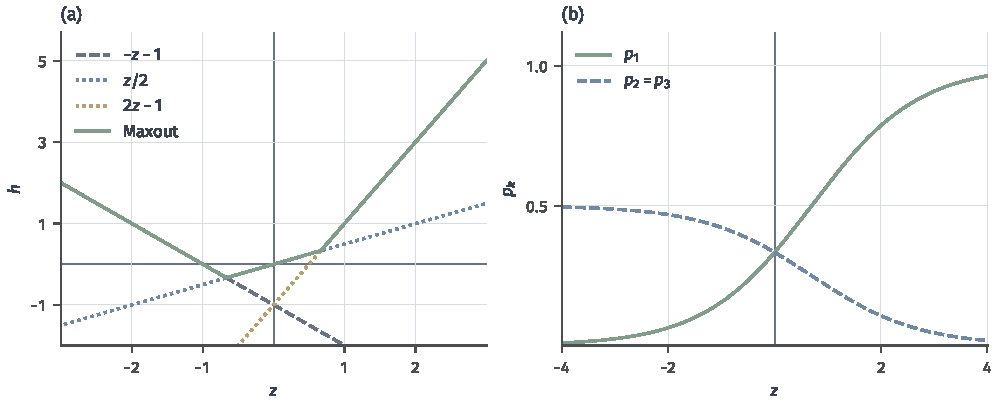
\includegraphics[width=159.059mm]{figures/05-neural-network-models/00-shared/matplotlib/ffn-activation-vector/figure.pdf}
  \caption{Maxout和Softmax的一维观察方式。左图取三个仿射候选$-z-1$、$0.5z$和$2z-1$，粗实线是它们的最大值包络；它展示固定参数后沿一维输入的Maxout响应。右图固定三类得分为$(z,0,0)$，绘出三项Softmax概率，其中$p_2=p_3$，用同一条曲线标注。这些切片不能代表所有输入与参数下的唯一函数图像。}
  \label{fig:ffn-activation-vector}
\end{figure*}

\subsubsection{激活函数的比较与选择}
\label{sec:ffn-activation-selection}

表~\ref{tab:ffn-activation-bounded}归纳了前面的有界响应与整流函数，表~\ref{tab:ffn-activation-smooth}补充指数型、自门控与向量变换。两表中的输出范围对应该层的任务约束，导数特点说明哪些输入区间能传递学习信号，参数与随机机制则说明响应怎样取得。曲线比较只呈现固定参数下的形状，训练还包括参数更新或随机采样。



\begin{table*}[htb]
  \centering
  \small
  \begin{tabularx}{\linewidth}{@{}l l X X@{}}
    \toprule
    函数 & 输出范围 & 导数与参数特点 & 适用场景及主要边界 \\
    \midrule
    ELU & $(-\alpha,+\infty)$ & 负端导数趋零，$\alpha$固定 & 允许负响应；零均值没有无条件保证 \\
    SELU & $(-\kappa\alpha,+\infty)$ & 固定缩放与负指数响应 & 自归一化MLP；需配套统计条件 \\
    Softplus & $(0,+\infty)$ & 平滑，导数为Sigmoid & 正尺度输出、平滑隐藏层；无精确零 \\
    Swish／SiLU & 依赖$\beta$ & $\beta$固定或学习，SiLU取$1$ & 平滑隐藏层、前馈模块；局部可非单调 \\
    GELU & 有负下界，正端无界 & 平滑，精确式或近似式 & Transformer前馈模块；非随机采样 \\
    Mish & 有负下界，正端无界 & 平滑，复合运算 & 视觉或其他隐藏层；收益需验证 \\
    Hardswish & $[-3/8,+\infty)$ & 两个分段边界 & 移动端响应；速度取决于实现 \\
    Maxout & 依赖候选仿射响应 & 选中分支获梯度，$K$套参数 & 学习分段函数；分支可能少获梯度 \\
    Softmax & 概率单纯形内部 & 联合依赖全部得分 & 互斥类别、归一化权重；非逐坐标激活 \\
    \bottomrule
  \end{tabularx}
  \caption{指数型、自门控与向量变换的比较。Swish在$\beta=0$时是线性函数；其余正$\beta$情形具有有限负下界。Softmax按$K\geq2$书写，输出各项严格为正且总和为$1$。表中的平滑性描述固定参数的标量函数，不能替代整条计算路径的可微性检查。}
  \label{tab:ffn-activation-smooth}
\end{table*}

若该层预测概率或正尺度，输出约束通常决定选择：互斥类别用Softmax，多个可共存标签分别用Sigmoid，正尺度可以用Softplus。若该层构造隐藏表示，则需要比较非线性、活动范围与梯度。ReLU提供简单的分段响应，Leaky ReLU与PReLU保留负梯度，GELU与SiLU提供平滑过渡；SELU与特定初始化和统计条件配套，采用它时需要同时确定这些条件。

计算成本也必须放回实现环境。分段线性函数少用指数等运算，但向量化、融合算子和内存访问可能改变实际耗时。平滑函数可用于需要连续导数的模型，其导数仍可能在某些输入区间很小；增加可学习斜率也可能改变初始化时的合适尺度。比较预测性能时，应固定数据划分、结构和评价口径，并说明是否重新调节学习率与初始化，才能区分激活变化和配套设置变化的影响。

% 历史开篇的两条完整边注文献需要与段落一起容纳。
\Needspace{16\baselineskip}
\subsubsection{从阈值单元到平滑门控：发展脉络}
\label{sec:ffn-activation-history}

McCulloch与Pitts在1943年把神经活动的“全或无”性质写成阈值单元；Rosenblatt在1958年的感知机工作中进一步讨论了连接如何从样本中调整\scite{mcculloch1943,rosenblatt1958}这些早期模型用单元的开关组合表达判定。硬阈值便于表达逻辑关系，但其普通导数几乎处处为零，无法直接承担本章所用的多层梯度学习。

当隐藏层需要通过损失学习表示时，连续响应提供了可用的局部导数。Rumelhart、Hinton与Williams在1986年的反向传播论文中使用Logistic响应，展示了隐藏单元怎样随训练形成特征。这一工作将可微的连续响应与隐藏表示的学习结合起来，使激活函数的选择与训练机制紧密相连\scite{rumelhart1986}

Sigmoid与Tanh随后也暴露出深层训练的尺度问题：两端饱和时，导数会变小，Sigmoid在原点附近的输出又以二分之一为中心。2010年Glorot与Bengio的工作把激活响应与初始化放在一起分析，考察了单元可导之外的传播条件：活动值和梯度经过多层之后是否仍有合适尺度。Tanh把输出中心移到零附近，但仍保留两端饱和的边界\scite{glorot2010initialization}

这里的“中心”指响应曲线在原点附近的位置：Sigmoid满足$s(0)=1/2$，Tanh满足$\tanh(0)=0$，后者的正负输出范围还关于零对称。若输入分布本身偏向一侧，输出仍可能有非零均值；只有加入前面所述的对称输入分布等条件，曲线的对称性才能进一步推出输出均值为零。

这项工作的对照还表明，即使保留同一种激活，改变权重初始化方式也会改变各层活动值与梯度的尺度。选择激活函数时，因而还要把初始化和层深放在一起考察：一条曲线的局部斜率不足以描述整条网络的训练状态。第~\ref{sec:ffn-initialization}节将从信号的二阶矩出发解释这种配合，区分Tanh的中心响应与ReLU的半轴截断。

整流函数让设计重点转向稀疏响应和正半轴上的线性传播。Nair与Hinton在2010年研究了受限玻尔兹曼机中的整流单元；Glorot、Bordes与Bengio在2011年进一步比较深层前馈网络的整流与Tanh响应。这两项工作分别在生成模型与深层判别网络中展示了整流响应的作用。正半轴不饱和缓解了一类梯度衰减，负半轴的零导数又促使后续方法保留泄漏斜率或允许负响应\scite{nair2010rectifiers,glorot2011rectifiers}

较新的分支把注意力转向平滑过渡与输入相关的门控。2016年的GELU按输入幅度平滑加权；2017年的Swish工作通过函数搜索研究自门控响应，并与ReLU比较。两者都保留较大的正响应，同时用平滑过渡替代正负区域之间的硬切换\scite{hendrycks2016gelu,ramachandran2017swish}

本节介绍的带斜率变体、指数响应和硬近似，分别延伸了可学习形状、信号尺度与计算成本这些方向。历史上的改进解决的是特定结构和训练设置中的问题；这些设置也构成今天复用相应结果时的条件。Sigmoid和Softmax在概率输出中的用途，则由预测对象决定，并不因隐藏层采用ReLU或平滑门控而消失。

\subsection{输出和学习目标}
\label{sec:ffn-output-objectives}

前面的隐藏层把输入变成了表示$\bm h^{(L)}$。但表示本身不是答案：要让网络完成任务，还必须回答两个问题——网络末端输出的数字\emph{代表什么}，以及用什么标准\emph{评判}这些数字与真实标签的差距。这部分末端计算称为输出头（output head）：它先用可学习的权重和偏置从隐藏表示算出若干个原始得分$\bm a$，再用一个由任务性质决定的变换$g$把得分变成有意义的预测量。

之所以需要不同的输出头，是因为不同任务要预测的对象在数学性质上不同：房价可以是任意实数，邮件是否垃圾邮件是一个“是/否”概率，手写数字是十个互斥类别中的一个，一篇文章的主题标签则可以同时成立多个。用同一套末端处理这些不同对象，要么得到没有意义的数值（比如对类别号直接做平方误差），要么无法表达必要的约束（比如概率必须落在$[0,1]$且互斥类别概率之和为$1$）。因此输出变换$g$不是可以随意选择的装饰，而是任务语义的一部分；与之配套的损失函数则决定训练信号。训练时可以让隐藏层与输出头一起调整，也可以在复用已训练网络时冻结隐藏层、只学习新任务的输出头。

同一组隐藏坐标可以接不同的输出头。图~\ref{fig:ffn-output-heads}比较连续数值、二分类、多类、多标签和表示输出五种方案；各头有各自的参数与损失，图中分支表示可替换的选择。下面按“原始得分长什么样、变换成什么预测量、用什么损失计分、如何据此作决策”这条统一线索，依次介绍这些输出头。

\begin{figure*}[!htb]
  \centering
  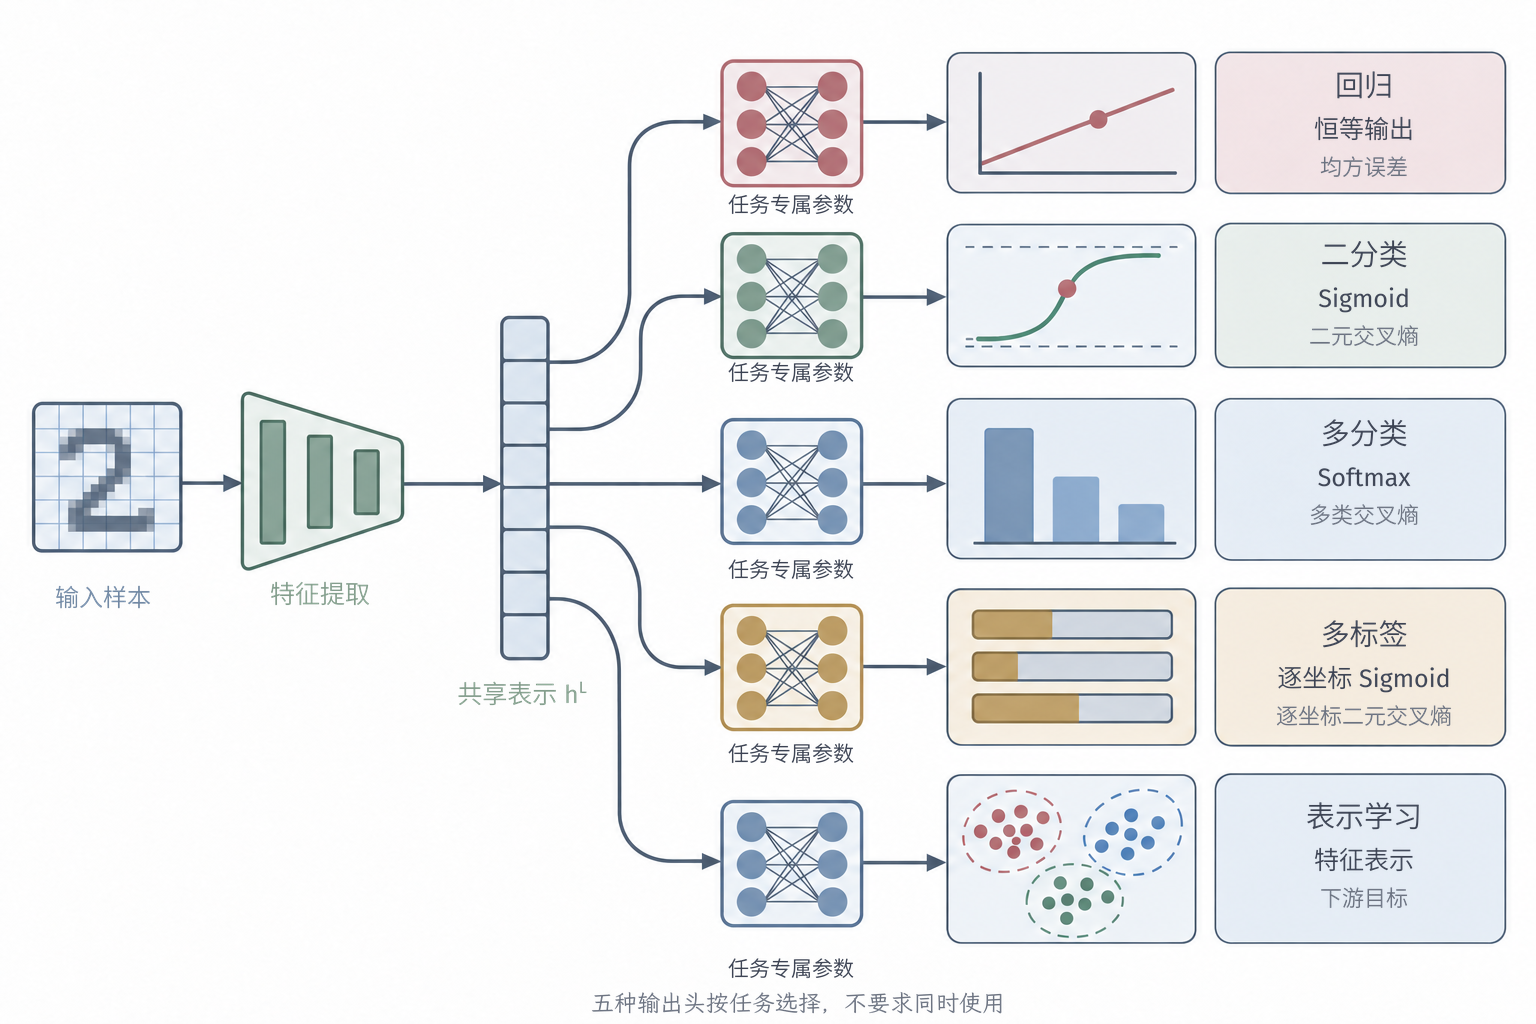
\includegraphics[width=130.048mm]{figures/05-neural-network-models/00-shared/generated/ffn-output-heads/figure.png}
  \caption{共同的前馈结构与五种可替换的输出头。左侧输入单元经隐藏单元形成$\bm{h}^{(L)}$；汇合线传递整组隐藏坐标，不执行求和。右侧单元产生各任务自己的原始得分，每个单元都读取全部隐藏坐标，并具有独立的输出权重与偏置。回归与二分类头只需一个得分；多类分类头联合归一化，多标签分类头逐坐标变换；表示头产生由下游任务约束的表示。向量头仅画三个坐标示意，实际维度由任务决定。右侧文字区分预测量与训练目标，隐藏激活无需与输出变换相同。}
  \label{fig:ffn-output-heads}
\end{figure*}

\subsubsection{回归：预测连续数值}
\label{sec:ffn-output-regression}

回归预测连续数值，例如经过单位缩放的房价。对标量目标$y\in\mathbb R$，输出头只需产生一个得分$a$，即$q=1$。采用恒等变换$g(a)=a$时，预测值为$\widehat y=a$，可用平方损失衡量它与目标的偏差：
\begin{equation}
  \ell(a,y)=\frac12(a-y)^2,
  \qquad \frac{\partial\ell}{\partial a}=a-y\text{。}
  \label{eq:ffn-regression-loss}
\end{equation}
系数$1/2$简化导数，不改变仅有该损失时的最优预测。若目标为$2.5$、当前预测为$2$，损失为$0.125$，输出导数为$-0.5$；沿负梯度方向调整输出会使它增大并接近目标。多个连续目标可用向量输出和$\frac12\lVert\bm a-\bm y\rVert_2^2$，各坐标的单位与尺度应在数据处理或损失权重中考虑。若要求严格正值预测，可以先令$\widehat y=\operatorname{Softplus}(a)$，再对变换后的预测计算损失。

\subsubsection{二分类：预测一个正类概率}
\label{sec:ffn-output-binary}

二分类判断一个事件是否成立，例如邮件是否属于垃圾邮件。令$y\in\{0,1\}$，其中$1$表示正类。这里希望网络给出的不是一个无界实数，而是“属于正类的概率”，概率必须落在$[0,1]$区间。但输出层算出的原始得分$a$可以是任意实数（很大的正数或很负的数），因此需要一个把整条实数轴单调压进$(0,1)$的变换。输出头产生一个实数$a$，经Sigmoid得到
\[
  p=s(a),\qquad P_{\bm\theta}(y=1\mid\bm x)=p,\qquad
  P_{\bm\theta}(y=0\mid\bm x)=1-p\text{。}
\]
$a$称为\term{logit}，即对数几率$\log(p/(1-p))$；它可以取任意实数，$p$才是正类概率。在这个伯努利模型下，正确标签的概率为$p^y(1-p)^{1-y}$，取负对数得到二元交叉熵：
\begin{equation}
  \begin{aligned}
    \ell(a,y)
      &=-y\log p-(1-y)\log(1-p)\\
      &=\log(1+\exp(a))-ya\text{。}
  \end{aligned}
  \label{eq:ffn-binary-cross-entropy}
\end{equation}
第二行利用$\log p=a-\log(1+\exp(a))$与$\log(1-p)=-\log(1+\exp(a))$，把两个对数项合并。对这一原始得分形式求导，就得到后续反向传播所用的起点：
\[
  \frac{\partial\ell}{\partial a}
  =\frac{\exp(a)}{1+\exp(a)}-y=p-y\text{。}
\]
例如正例的$p$从$0.8$降到$0.2$时，损失从约$0.2231$增到$1.6094$，说明损失会区分分给正确标签的概率。预测类别还需规定阈值$\tau$，如按$p\geq\tau$判正类；阈值应结合误判代价与验证指标选择。学习时使用连续损失，作出类别决策时才应用阈值。

\subsubsection{互斥多分类：预测一个类别}
\label{sec:ffn-output-multiclass}

若样本恰好属于$K$类中的一类，例如一张数字图像对应“0到9”中的某一个数字类别，就让输出头产生$K$个得分$a_1,\ldots,a_K$，即$q=K$。互斥意味着这$K$个概率必须满足两个条件：每个都非负，且加起来恰好等于$1$（样本必定属于其中某一类）。如果对每个得分分别用Sigmoid，得到的$K$个数之间没有这种竞争关系，它们之和既不等于$1$、也无法直接解释成一个概率分布。Softmax通过一次共同归一化来建立这种竞争：标签为$y\in\{1,\ldots,K\}$，Softmax把得分共同转换为互斥类别的概率，并按最大概率判类：
\begin{equation}
  p_k=\frac{\exp(a_k)}{\sum_{j=1}^{K}\exp(a_j)},
  \qquad \sum_{k=1}^{K}p_k=1,\qquad
  \widehat y=\operatorname*{arg\,max}_{k}p_k\text{。}
  \label{eq:ffn-multiclass-output}
\end{equation}
最大概率并列时需预先固定决策规则。正确标签的概率是$p_y$，取负对数得到多类交叉熵：
\begin{equation}
  \ell(\bm{a},y)=-\log p_y
  =-a_y+\log\sum_{j=1}^{K}\exp(a_j)\text{。}
  \label{eq:ffn-multiclass-cross-entropy}
\end{equation}
对$a_k$求导时，$-a_y$贡献$-\mathbb I\{y=k\}$，其中指示函数在$y=k$时为$1$，否则为$0$；对数求和项贡献$\exp(a_k)/\sum_j\exp(a_j)=p_k$。两项相加，得分梯度就是$p_k-\mathbb I\{y=k\}$。因此正确类得分的负梯度方向为正，其他类为负；这些信号怎样调整输出权重及隐藏表示，将由反向传播计算。

\subsubsection{多标签分类：预测多个二值结果}
\label{sec:ffn-output-multilabel}

同一文档可以同时属于“技术”和“教育”，这类任务需要分别判断多个标签是否成立。与互斥多分类相反，这里的标签之间没有竞争关系：一个标签成立不会挤占其他标签成立的可能，因此不能用Softmax强制概率之和为$1$，而应对每个标签各设一个独立的“是/否”判断。\term{多标签分类}（multi-label classification）使用目标$\bm y\in\{0,1\}^{K}$，输出头对每个得分分别使用Sigmoid，再把各标签的二元交叉熵相加：
\begin{equation}
  \begin{aligned}
    p_k&=s(a_k),\\
    \ell(\bm{a},\bm{y})
      &=\sum_{k=1}^{K}\bigl[-y_k\log p_k-(1-y_k)\log(1-p_k)\bigr]\\
      &=\sum_{k=1}^{K}\bigl[\log(1+\exp(a_k))-y_k a_k\bigr]\text{。}
  \end{aligned}
  \label{eq:ffn-multilabel-loss}
\end{equation}
这些概率不必加起来等于$1$。例如$\bm p=(0.8,0.7,0.1)^{\top}$，按各标签的阈值$0.5$决策，会选出前两个标签。每一项沿用二分类损失，所以每个得分的梯度仍为$p_k-y_k$；不同标签也可以分别选择阈值。这两种任务都可输出$K$维向量，标签是否允许共存决定使用Softmax还是逐坐标Sigmoid。

\subsubsection{表示输出：由下游目标提供约束}
\label{sec:ffn-output-representation}

输出也可以继续交给其他模块使用。例如，下游模块需要的表示维度与$\bm h^{(L)}$不同，输出头便先把它映射为$\bm a\in\mathbb R^q$，再作为表示$\bm r$供分类、比较或重建使用。可以直接取$\bm r=\bm a$；若任务只比较向量方向，则在$\bm a\neq\bm0$时归一化为
\begin{equation}
  \bm{r}=\frac{\bm{a}}{\lVert\bm{a}\rVert_2}\text{。}
  \label{eq:ffn-normalized-representation}
\end{equation}
例如$(3,4)^{\top}$变为$(0.6,0.8)^{\top}$，保留方向、去掉整体长度差异。归一化只规定长度，表示应保留什么信息仍需由使用目标确定：接分类头时由分类损失约束表示，用于重建时由重建误差约束表示。联合训练时，这些损失的梯度经过下游模块传回表示网络，使输出坐标接受使用任务的约束。

\subsubsection{从单样本损失到训练目标}
\label{sec:ffn-empirical-objective}

前面已经规定了一条样本怎样预测、怎样计分，学习则要让同一组参数服务于整个训练集。设$S=((\bm x_i,\bm y_i))_{i=1}^{n}$，标量标签按对应任务书写，网络对第$i$个输入产生原始得分$\bm a_i(\bm\theta)$。汇总各样本损失，并加入可选的参数惩罚，得到
\begin{equation}
  J_S(\bm{\theta})=
  \frac1n\sum_{i=1}^{n}\ell\!\left(\bm{a}_i(\bm{\theta}),\bm{y}_i\right)
  +\lambda\Omega(\bm{\theta})\text{。}
  \label{eq:ffn-training-objective}
\end{equation}
这里$\ell$已包含任务的输出变换，$\Omega$是参数惩罚，$\lambda\geq0$控制惩罚强度；表示输出的损失则来自相连的下游目标。固定隐藏层时，其参数保持不变，只调整输出头；联合训练时，两部分参数共同参与同一目标的更新。输出范围由$g$规定，训练依据由损失给出；对于分类任务，阈值或最大概率规则再把预测用于具体决策。

\section{参数学习}
\label{sec:ffn-learning}

结构和损失规定了“网络长什么样、什么算好”，但训练开始时表里还没有填入合适的数值。要真正学到参数，还要解决两个工程与数学上都无法回避的问题。第一个是\emph{起点}：在看到任何数据之前，权重应当初始化成什么？全部置零看似自然，却会导致致命的对称问题；随机赋值则要进一步考虑数值取多大才合适。第二个是\emph{方向}：网络可能有几百万、上亿个参数，每更新一次，都要知道每个参数应当增大还是减小、变动多少，手工推导显然不可行，这就需要一套能机械执行的求导算法——反向传播。初始化决定从参数空间的哪个位置出发，反向传播决定每一步朝哪个方向走，自动微分则让程序能够自动完成这些求导；至于沿这个方向走多大一步（学习率）、用什么优化策略走，则属于求出梯度之后的优化问题。

\subsection{参数初始化}
\label{sec:ffn-initialization}

初始化要同时满足两个看起来独立、实则相关的要求：让同层单元“各不相同”，并让信号和梯度在层间传播时“尺度不失控”。第一点针对对称性，第二点针对数值幅度。下面先说明为什么这两点都不可省略，再据此结合每层的连接数推导合适的权重方差。

\subsubsection{共同要求：打破对称并控制尺度}
\label{sec:ffn-initialization-common}

先看对称性为什么是致命的。假设一层里所有单元的输入权重、偏置完全相同，并且它们通向下一层的连接也对称，那么无论输入什么，这一层所有单元的输出都相同；反向传播时，它们收到的梯度也完全相同，于是更新之后权重仍然相同。这种对称性一旦建立就会被每一步更新严格保持下去：一个有$64$个单元的隐藏层，实际上永远只在重复计算同一个特征，等价于只有一个单元，网络的容量被白白浪费。全零初始化正是这种完全对称的起点。因此权重必须随机初始化，使各单元一开始就关注不同的输入方向；偏置不参与打破这种方向对称，通常可以置零（或按输出层的需要单独设置）。

打破对称只解决了“各不相同”，还没有解决“取多大”。若权重普遍过大，加权和的绝对值会很大，Sigmoid、Tanh单元随即进入两端几乎水平的饱和区；若权重普遍过小，信号逐层衰减，深层单元的输入几乎相同、难以区分，梯度也会随之变得微弱。合适的幅度应当与该单元读取的输入个数相联系。设输入坐标具有共同且有限的二阶矩$q_{\mathrm{in}}=\mathbb E[u_k^2]$，初始权重独立、均值为零、方差为$v$，整组权重与整组输入独立，偏置为零。把$m$个输入的加权和$z=\sum_{k=1}^{m}w_k u_k$平方展开，有
\[
  \mathbb E[z^2]
  =\sum_{k=1}^{m}\mathbb E[w_k^2u_k^2]
    +2\sum_{k<j}\mathbb E[w_k w_j u_k u_j]\text{。}
\]
对角项为$\mathbb E[w_k^2]\mathbb E[u_k^2]=v q_{\mathrm{in}}$；交叉项含有$\mathbb E[w_k w_j]=0$，即使输入坐标彼此相关也会消失。因此
\begin{equation}
  \mathbb{E}[z^2]=m v q_{\mathrm{in}}\text{。}
  \label{eq:ffn-initial-signal-scale}
\end{equation}
若激活近似保留预激活的二阶矩，取$m v\approx1$就使本层输出与输入的二阶矩接近；激活进一步压缩或截断响应时，还要计入相应因子。

输入连接数$m=d_{\ell-1}$称为\term{fan-in}；同一输入坐标通向的输出连接数$d_\ell$称为\term{fan-out}。前者决定一个输出汇总多少输入，后者决定一个输入在反向计算中接收多少下游贡献。

\subsubsection{饱和激活的尺度：Glorot初始化}
\label{sec:ffn-initialization-saturating}

对于前面讨论的饱和激活，过大的初始预激活容易进入小导数区域。增大权重虽然能放大仿射结果，也可能把更多单元推入饱和区，因此不能只靠放大权重补偿小导数。先以Tanh原点附近的近似单位斜率为基准，估计前、后两个方向的传播尺度。

记最终标量损失对本层输出预激活$z_j$的敏感度为$\gamma_j$，其共同二阶矩为$q_{\mathrm{back}}$。一个输入$u_k$接收$d_\ell$个输出的影响，链式法则给出
\[
  \widetilde\gamma_k
  :=\frac{\partial\ell}{\partial u_k}
  =\sum_{j=1}^{d_\ell}(\bm W_\ell)_{j,k}\gamma_j\text{。}
\]
暂把本层权重与整组下游敏感度视为独立，平方展开中的交叉项便消失，每个对角项为$v q_{\mathrm{back}}$，得到$\mathbb E[\widetilde\gamma_k^2]\approx d_\ell v q_{\mathrm{back}}$。这里的独立性是忽略实际依赖的尺度近似，故对真实网络使用近似等号。

前向和后向的传播因子分别为$d_{\ell-1}v$与$d_\ell v$。两侧宽度不同时，不能用同一个$v$让它们都等于$1$；一种折中是令两因子的算术平均为$1$，即$((d_{\ell-1}+d_\ell)/2)v=1$。\term{Glorot初始化}（Glorot initialization，也称Xavier初始化）由此采用
\begin{equation}
  \begin{aligned}
    v&=\frac{2}{d_{\ell-1}+d_\ell},\\
    (\bm{W}_\ell)_{j,k}&\sim
    \mathcal{U}\!\left[-\sqrt{\frac{6}{d_{\ell-1}+d_\ell}},
    \sqrt{\frac{6}{d_{\ell-1}+d_\ell}}\right]\text{。}
  \end{aligned}
  \label{eq:ffn-glorot-initialization}
\end{equation}
其中$\mathcal U$表示均匀分布。对$a>0$，$\mathcal U[-a,a]$的方差为$\frac1{2a}\int_{-a}^{a}t^2\,\mathrm dt=a^2/3$，令它等于上述$v$，就得到式中的端点；也可以采用同方差的零均值正态分布。

改变激活时，还可按其传播作用调整初始权重的标准差，这个调整系数称为激活增益；标准差乘一个系数时，方差要乘其平方。Sigmoid的中心斜率更小，且具有非零输出中心，因此上述单位斜率近似不能直接覆盖它的传播；Glorot与Bengio的分析也考察了这些因素及饱和问题\scite{glorot2010initialization}

\subsubsection{ReLU及其变体：补偿被截断的响应}
\label{sec:ffn-initialization-rectifiers}

对于ReLU，需要补偿负半轴被截断的平方幅度。若预激活$z$关于零对称，正、负半轴的平方贡献相等；零点的平方贡献为零，所以即使零点具有正概率质量，仍有
\[
  \mathbb{E}[\rho(z)^2]=\frac12\mathbb{E}[z^2]\text{。}
\]
这是二阶矩关系；ReLU输出通常有正均值，方差还要减去均值平方。结合式\eqref{eq:ffn-initial-signal-scale}，激活后的二阶矩为$q_{\mathrm{out}}=(m v/2)q_{\mathrm{in}}$；要使$q_{\mathrm{out}}\approx q_{\mathrm{in}}$，可取$v\approx2/m$。相应的\term{He初始化}（He initialization，也称Kaiming初始化）采用
\begin{equation}
  (\bm{W}_\ell)_{j,k}\sim
  \mathcal{N}\!\left(0,\frac{2}{d_{\ell-1}}\right)\text{。}
  \label{eq:ffn-he-initialization}
\end{equation}

在同一对称分布下，初始化时若负半轴斜率固定为$\alpha$，正、负半轴分别贡献原二阶矩的$1/2$和$\alpha^2/2$，总因子为$(1+\alpha^2)/2$。因此，Leaky ReLU或PReLU初始斜率对应的前向权重方差为$2/((1+\alpha^2)d_{\ell-1})$；PReLU开始学习斜率后，这一初始补偿尺度也可能改变。

后向还需考察局部回传系数的平方平均。若预激活关于零对称且零点概率为零，ReLU两侧的系数平方分别为$1$和$0$，平均为$1/2$；带泄漏时为$(1+\alpha^2)/2$。在局部回传系数、权重与下游敏感度的独立性近似下，将这些因子乘入前面的后向求和估计，就得到把方差分母中的fan-in换成fan-out的方案。若零点有正概率质量，后向因子还取决于零点回传约定，不能仅由对称性确定\scite{he2015rectifiers}

\subsubsection{其他隐藏激活与任务输出：分别设置}
\label{sec:ffn-initialization-other}

其他隐藏激活应按自身响应和实现的增益约定选择尺度，SELU还需沿用前面说明的配套初始化与统计条件。输出层也按自己的运算设置：线性得分层没有半轴截断，无须自动继承ReLU隐藏层的系数$2$；二分类还应关注初始logit是否过大。

使用这些设置时，需要结合输入处理和层宽观察初始活动值与梯度。以上分布与独立性估计描述的是起点，训练后权重、表示和下游敏感度可能相关，仍需根据实际数值判断后续尺度。接下来的反向传播将具体说明这些敏感度怎样计算并用于参数更新。

\subsection{反向传播}
\label{sec:ffn-backpropagation}

初始化解决了起点问题，现在解决训练的核心问题。输出层的参数容易处理：它的输出直接参与损失，预测偏高就把相关权重调低、偏低就调高。隐藏层却不同——我们从不为隐藏单元提供目标值，没有人告诉某个隐藏单元“你此刻应该输出$0.7$”。那么，怎样判断一个深处的隐藏权重应当增大还是减小？

答案来自一个朴素的追问：这个隐藏单元的输出会影响谁？它影响下一层，下一层又影响再下一层……如此一路传到最终损失。因此，最终损失对某个隐藏量的敏感程度，可以沿着这条依赖链\emph{反向}逐层追踪回来：先知道损失对最末端输出有多敏感，再乘以“输出对倒数第二层的局部变化率”，得到损失对倒数第二层的敏感度；如此逐层向内，直到每个参数。这正是微积分中链式法则的系统性应用，称为\term{反向传播}（backpropagation）。

下面把反向传播展开为预激活敏感度、逐层递推、参数梯度与批量汇总四步。采用列向量梯度时，链式法则在矩阵形式上体现为Jacobian转置。

先固定一个样本，把输出变换与损失合为标量函数$\ell(\bm{a},\bm{y})$。用列向量表示梯度，定义
\begin{equation}
  \bm{\delta}^{(L+1)}=\nabla_{\bm{a}}\ell,
  \qquad
  \bm{\delta}^{(\ell)}=\nabla_{\bm{z}^{(\ell)}}\ell
  \quad(\ell=1,\ldots,L)\text{。}
  \label{eq:ffn-delta-definition}
\end{equation}
向量$\bm{\delta}^{(\ell)}\in\mathbb{R}^{d_\ell}$记录损失对本层各预激活坐标的敏感程度。“误差”是这一敏感度的常用名称；其数值来自最终损失的导数，而隐藏层通常没有直接指定的标签。

在可微点，这些敏感度由普通导数给出。ReLU在零点没有普通导数，但训练程序仍需规定遇到该值时怎样回传。本章的ReLU计算采用下面的局部回传系数：
\[
  D_\rho(z)=
  \begin{cases}
    1,&z>0,\\
    0,&z\leq0\text{。}
  \end{cases}
\]
它在两个开半轴上等于ReLU导数，在零点取$0$是一项实现约定，不表示该点存在普通导数。以下递推中，对ReLU原本填写$\rho'(z)$的位置使用$D_\rho(z)$；其他分段激活也要把拐点处的回传规则连同函数定义一起固定。Maxout不是这里的逐坐标激活，它还需规定并列最大时把敏感度分配给哪些分支；这些算子规则是网络计算的一部分。

由式\eqref{eq:ffn-output-map}，输出得分对$\bm{h}^{(L)}$的Jacobian矩阵为$\bm{W}_{L+1}$，
所以损失对最后一个隐藏表示的梯度为$\bm{W}_{L+1}^{\top}\bm{\delta}^{(L+1)}$。
隐藏激活逐坐标作用，其Jacobian矩阵以各坐标导数为对角元素。
把两步链式法则合起来，便得到逐层递推：
\begin{equation}
  \bm{\delta}^{(\ell)}=
  \left(\bm{W}_{\ell+1}^{\top}\bm{\delta}^{(\ell+1)}\right)
  \odot\sigma_\ell'\!\left(\bm{z}^{(\ell)}\right),
  \qquad \ell=L,\ldots,1\text{。}
  \label{eq:ffn-backward-recursion}
\end{equation}
其中$\odot$表示逐坐标乘法。这个递推式虽然紧凑，却只是两步直觉的合并，可以拆开读。第一步$\bm{W}_{\ell+1}^{\top}\bm{\delta}^{(\ell+1)}$回答“后层有多怪罪本层”：后层每个单元的敏感度，按它们与本层各单元的连接权重加权汇总回来，所以用权重矩阵的转置。第二步再逐坐标乘上$\sigma_\ell'(\bm{z}^{(\ell)})$，回答“本层单元自己放行多少”：如果单元正处在激活函数平缓（导数接近零）的区域，即使后层很不满意，这个不满也很难通过该单元传回到它的输入权重。两步合起来，就得到损失对本层预激活值的敏感度。递推中的每个向量维度都是$d_\ell$，因此可逐层核对矩阵形状是否匹配。

这里维度为$d_\ell$的是当前层的递推结果，以及相乘前已经汇总到当前层的向量。后层敏感度$\bm\delta^{(\ell+1)}$本身属于$\mathbb R^{d_{\ell+1}}$；先乘形状为$d_\ell\times d_{\ell+1}$的$\bm W_{\ell+1}^{\top}$，才得到可与本层激活导数逐坐标相乘的$d_\ell$维向量。

参数的导数来自本层仿射运算。对任一层$\ell=1,\ldots,L+1$，第$j$个预激活值对权重$(\bm{W}_\ell)_{j,k}$的导数是$h_k^{(\ell-1)}$，对偏置$(\bm{b}_\ell)_j$的导数是$1$。由此得到
\begin{equation}
  \nabla_{\bm{W}_\ell}\ell
    =\bm{\delta}^{(\ell)}(\bm{h}^{(\ell-1)})^{\top},
  \qquad
  \nabla_{\bm{b}_\ell}\ell=\bm{\delta}^{(\ell)}\text{。}
  \label{eq:ffn-parameter-gradients}
\end{equation}
第一式是一个外积：每条连接的梯度等于目标单元的损失敏感度乘以来源单元的活动值。矩阵形状为$d_\ell\times d_{\ell-1}$，恰好与权重相同。对输入的梯度则为$\nabla_{\bm{x}}\ell=\bm{W}_1^{\top}\bm{\delta}^{(1)}$；即使输入不参与参数更新，这个量也能用于分析预测对输入变化的敏感程度。

输出层的起点由任务决定。采用式\eqref{eq:ffn-regression-loss}时，$\delta^{(L+1)}=a-y$；采用二元交叉熵时，$\delta^{(L+1)}=p-y$；采用多类交叉熵时，第$k$个坐标为$p_k-\mathbb{I}\{y=k\}$，其中$\mathbb{I}$是事件成立时为$1$的指示函数。概率输出与交叉熵合并后得到的简洁导数，是两者配合的结果。若Sigmoid输出后使用平方损失，导数还包含$s'(a)$，此时$p-y$还需乘上述输出变换导数。

图~\ref{fig:ffn-backpropagation}把下面算例的$2$-$3$-$1$网络展开，说明前向值与反向梯度的区别。前向计算提供各层的预激活和表示；反向计算从损失开始，重复利用这些值与局部导数。梯度向上游传播不会改变本次前向预测已经使用的输入，也不会给预测网络增加有向环。

\begin{figure*}[htb]
  \centering
  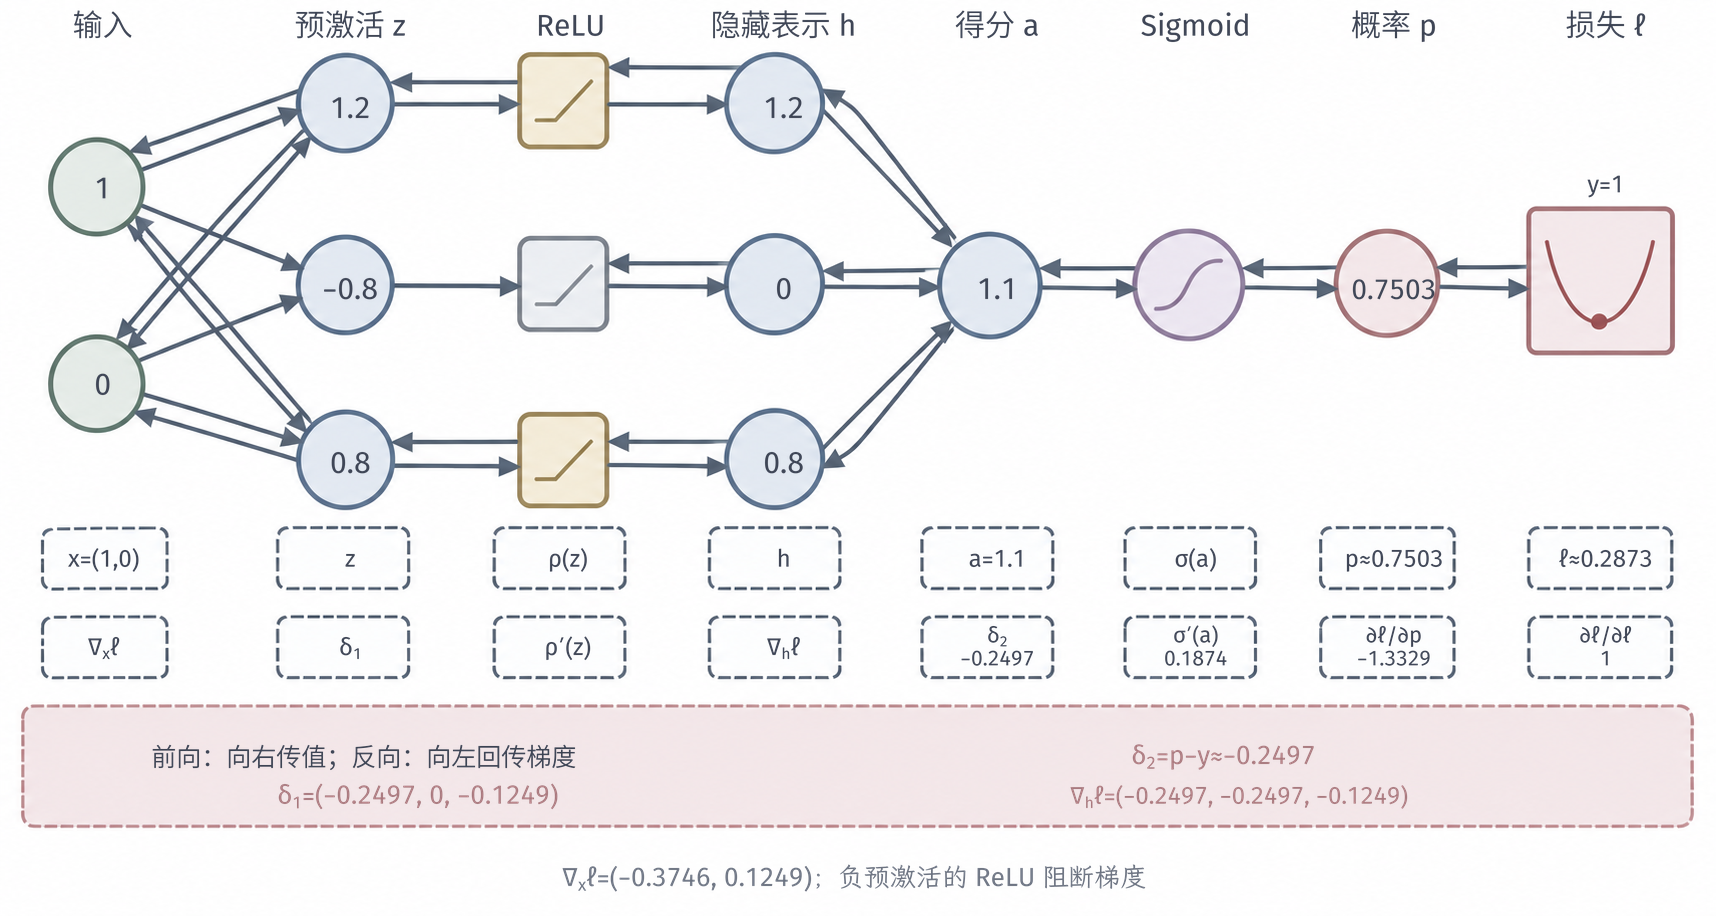
\includegraphics[width=145.288mm]{figures/05-neural-network-models/00-shared/generated/ffn-backpropagation/figure.png}
  \caption{示例~\ref{ex:ffn-numerical-backpropagation}中$2$-$3$-$1$网络的计算图。上方节点和下方第一行给出前向值，第二行及红色汇总给出反向量；箭头方向区分前向传值与反向回传梯度；预激活与隐藏表示是同一隐藏层的两种数值，不是两个隐藏层。下方红色虚线按向量形式汇总梯度，坐标顺序与上方节点从上到下一致。第三个单元通过输出权重$0.5$收到梯度，第二个单元的梯度被负半轴上的ReLU截断。数值按更新前参数计算，梯度和概率保留四位小数。}
  \label{fig:ffn-backpropagation}
\end{figure*}

\begin{example}[一次前向与反向计算]
  \label{ex:ffn-numerical-backpropagation}
  沿用异或的二值输入，使用图~\ref{fig:neural-minimal-mlp}中的$2$-$3$-$1$结构：一个隐藏层含三个ReLU单元，输出得分经Sigmoid变成二分类概率。下面的参数是教学构造，不是已训练好的异或分类器：
  \[
    \begin{aligned}
      \bm{W}_1&=\begin{pmatrix}1&-1\\-1&1\\1&1\end{pmatrix},
      &\bm{b}_1&=\begin{pmatrix}0.2\\0.2\\-0.2\end{pmatrix},\\
      \bm{W}_2&=\begin{pmatrix}1&1&0.5\end{pmatrix},
      &b_2&=-0.5\text{。}
    \end{aligned}
  \]
  对样本$\bm{x}=(1,0)^{\top}$、$y=1$，前向结果为
  \[
    \begin{aligned}
      \bm{z}^{(1)}&=(1.2,-0.8,0.8)^{\top},\\
      \bm{h}^{(1)}&=(1.2,0,0.8)^{\top},\\
      a&=1\times1.2+1\times0+0.5\times0.8-0.5=1.1\text{。}
    \end{aligned}
  \]
  因而$p=s(1.1)\approx0.7503$，二元交叉熵$\ell=-\log p\approx0.2873$。本例三个预激活值都远离ReLU的不可微点，局部导数依次为$1,0,1$。

  输出敏感度为$\delta^{(2)}=p-1\approx-0.2497$。先乘输出权重的转置，再逐坐标乘激活导数，得到
  \[
    \begin{aligned}
      \nabla_{\bm{h}^{(1)}}\ell
        &\approx(-0.2497,-0.2497,-0.1249)^{\top},\\
      \bm{\delta}^{(1)}&\approx(-0.2497,0,-0.1249)^{\top},\\
      \nabla_{\bm{W}_1}\ell&\approx
      \begin{pmatrix}-0.2497&0\\0&0\\-0.1249&0\end{pmatrix},
      &\nabla_{\bm{b}_1}\ell&\approx
      \begin{pmatrix}-0.2497\\0\\-0.1249\end{pmatrix}\text{。}
    \end{aligned}
  \]
  例如第三个隐藏单元的第一条输入权重，其梯度是
  \[
    \frac{\partial\ell}{\partial(\bm{W}_1)_{3,1}}
    =(p-1)\times0.5\times1\times x_1
    \approx-0.1249\text{。}
  \]
  这四个因子依次来自输出损失、输出连接、ReLU局部导数和输入值。输出参数的梯度为$\nabla_{\bm{W}_2}\ell\approx(-0.2997,0,-0.1998)$、$\partial\ell/\partial b_2\approx-0.2497$；继续回传到输入则有$\nabla_{\bm{x}}\ell\approx(-0.3746,0.1249)^{\top}$。第一层第一、第三个单元对$x_2$的权重梯度为零，是因为这个样本的$x_2=0$；第二个单元的输入权重梯度为零，则来自负半轴上的激活导数。两种零梯度有不同原因。

  若仅用该样本、不加正则项，并以学习率$0.1$同时更新所有参数，即每项参数减去$0.1$倍的对应梯度，则更新后的参数为
  \[
    \begin{aligned}
      \bm{W}_1^{(1)}&\approx
        \begin{pmatrix}1.0250&-1\\-1&1\\1.0125&1\end{pmatrix},
      &\bm{b}_1^{(1)}&\approx
        \begin{pmatrix}0.2250\\0.2\\-0.1875\end{pmatrix},\\
      \bm{W}_2^{(1)}&\approx\begin{pmatrix}1.0300&1&0.5200\end{pmatrix},
      &b_2^{(1)}&\approx-0.4750\text{。}
    \end{aligned}
  \]
  参数上标$(1)$表示一次更新。用未舍入的梯度重算该输入，隐藏表示约为$(1.2499,0,0.8250)^{\top}$，得分约为$1.2414$，正类概率约为$0.7758$，损失约为$0.2539$。本次下降只针对更新所用的正例；全部异或样本的总损失与新样本风险，需要分别用相应样本或分布评价。
\end{example}

上面的求导针对一条样本，但一次参数更新是否必须看完整个训练集？如果每次更新都精确计算式\eqref{eq:ffn-training-objective}的数据梯度，就要用当前参数遍历全部$n$个训练样本；在数百万样本的数据集上，这意味着每走一小步都要完整扫描一遍数据，训练慢得无法接受。一个自然的折衷是：每步只随机读取一小部分样本，用这批样本上的平均梯度近似全体样本的梯度。数据较多时，这样既能大幅减少一次更新的计算与中间值存储，又因为频繁更新而往往收敛得更快。为给这种做法规定一种明确含义，并说明“近似”在什么意义下成立，下面取固定批量大小$b$，满足$1\leq b\leq n$；在每次更新的参数已经确定后，独立地从全部索引中均匀抽取$b$个不同索引。均匀指每个大小为$b$的子集具有相同的入选概率。

训练目标通常包含多个样本，它们共享同一组参数，因此梯度需要相加。若本次更新读取一个索引集合$B\subseteq\{1,\ldots,n\}$，称为\term{小批量}（mini-batch），其平均数据梯度为
\begin{equation}
  \bm{G}_\ell=
  \frac1{|B|}\sum_{i\in B}
  \bm{\delta}_i^{(\ell)}(\bm{h}_i^{(\ell-1)})^{\top},
  \qquad
  \bm{r}_\ell=
  \frac1{|B|}\sum_{i\in B}\bm{\delta}_i^{(\ell)}\text{。}
  \label{eq:ffn-minibatch-gradients}
\end{equation}
这里$\bm{G}_\ell\in\mathbb R^{d_\ell\times d_{\ell-1}}$是权重梯度矩阵，$\bm{r}_\ell\in\mathbb R^{d_\ell}$是偏置梯度向量。每个样本的$\bm{\delta}_i^{(\ell)}$按未除以批量大小的单样本损失计算。若反向起点已经使用批平均损失，所得敏感度已经包含按$|B|$取平均的缩放。矩阵实现可将样本按列排列，用同样的矩阵乘法一次计算这些外积之和；样本按行排列的实现会相应改变转置位置。

下文把按前述局部规则计算的单样本参数回传量称作数据梯度。各局部运算可微时，这些量就是普通梯度；遇到ReLU零点等非光滑位置时，则按已经固定的算子规则理解它们。接下来的抽样等式只利用这些已确定量的有限求和关系，并不据此断言非光滑位置存在普通梯度。

这里$B$必须非空，且上述抽样规则使$|B|=b$。固定训练集和本次更新前的参数$\bm\theta$，把第$i$个样本对全部参数的数据梯度记为$\bm g_i(\bm\theta)$。所有索引在均匀抽样中地位相同，而每次恰有$b$个索引入选，所以每个索引的入选概率为$b/n$。于是
\[
  \begin{aligned}
    \mathbb{E}_B\!\left[
      \frac1b\sum_{i\in B}\bm g_i(\bm\theta)
      \,\middle|\,\bm\theta\right]
      &=\frac1b\sum_{i=1}^{n}
        \mathbb{P}(i\in B\mid\bm\theta)\bm g_i(\bm\theta)\\
      &=\frac1n\sum_{i=1}^{n}\bm g_i(\bm\theta)\text{。}
  \end{aligned}
\]
因此，按这一规则计算的批平均梯度，在抽样平均意义下等于同一点的全数据梯度；一次具体抽样得到的梯度仍可能偏离它。非均匀选择样本时，若不按抽样概率作相应加权，就一般不能沿用这个等式。按既定顺序循环读取或随机打乱后顺次读取，也是需要另行分析的取样规则，不能把这里的条件期望结论直接套上去。

加上当前参数处确定的惩罚项梯度后，上述平均关系同样适用于完整训练目标的梯度估计。减少每次读取的样本数带来计算上的节省，也引入了抽样波动；即使批内损失因更新而降低，全数据目标也可能在这一步升高。这里给出的是梯度估计与原目标的关系，没有给出每次更新都降低全数据损失的保证。

若$\Omega=\frac12\sum_\ell\lVert\bm{W}_\ell\rVert_{\mathrm{F}}^2$，其中$\lVert\cdot\rVert_{\mathrm{F}}$是矩阵各元素平方和开方得到的Frobenius范数，则权重总梯度为$\bm{G}_\ell+\lambda\bm{W}_\ell$，未被惩罚的偏置不加这一项。给定学习率$\eta_t>0$，普通梯度更新为
\begin{equation}
  \begin{aligned}
    \bm{W}_\ell^{(t+1)}
      &=\bm{W}_\ell^{(t)}-\eta_t(\bm{G}_\ell+\lambda\bm{W}_\ell^{(t)}),\\
    \bm{b}_\ell^{(t+1)}&=\bm{b}_\ell^{(t)}-\eta_t\bm{r}_\ell\text{。}
  \end{aligned}
  \label{eq:ffn-gradient-update}
\end{equation}
这里迭代上标$t$与层下标$\ell$分别记录训练时刻和结构位置。

下面算法中的“读取小批量”采用上述非空均匀抽样规则，ReLU在零点按$D_\rho(0)=0$回传。采用其他激活或取样方式时，需要同时确定相应的算子规则和批量规则，再按同一前向计算求取梯度；这些约定与网络结构、损失一起构成可执行的训练设定。

\begin{algorithm}[前馈网络的小批量梯度学习]
  \label{alg:ffn-minibatch-learning}
  \begin{algorithmic}[1]
    \Require 训练集$S$、验证集、网络结构、损失、学习率序列与停止规则
    \Ensure 经验证集选择的参数$\bm{\theta}$
    \State 按激活与层宽初始化权重，初始化偏置
    \While{尚未达到停止规则}
      \State 读取小批量$B$，保存各样本的预激活、隐藏表示与输出
      \State 计算输出敏感度$\bm{\delta}_i^{(L+1)}$
      \For{$\ell=L,L-1,\ldots,1$}
        \State 按式\eqref{eq:ffn-backward-recursion}计算$\bm{\delta}_i^{(\ell)}$
      \EndFor
      \State 汇总所有层的数据梯度，并加入所选惩罚项的梯度
      \State 使用同一更新前参数计算的梯度，同时更新各层参数
      \State 按既定间隔评估验证集，记录待选择的参数
    \EndWhile
    \State 返回按预先规定验证指标选择的参数
  \end{algorithmic}
\end{algorithm}

算法~\ref{alg:ffn-minibatch-learning}把求导和更新分成两步。如果在尚未完成反向计算时就改写某层权重，前后各层的梯度可能对应不同的参数，便不再是同一个目标在同一点的梯度。停止规则可以包含最大更新次数和验证指标的停止条件；优化器、学习率安排及更广泛的训练问题将在训练章比较。

反向传播每层主要计算转置矩阵乘法和外积，计算量与一次前向同阶；它还要保存各层的活动值，单样本隐藏激活的存储量与$\sum_\ell d_\ell$同阶，小批量时随批量大小增长。

更重要的是，逐层递推中的连乘结构揭示了深层网络特有的训练风险。损失对最底层参数的梯度，等于沿途每一层“局部回传系数”的乘积再求和：如果这些系数普遍小于$1$，连乘会使梯度随层数急剧缩小，最底层几乎收不到学习信号；如果普遍大于$1$，连乘又会使梯度急剧放大。这两种现象分别称为梯度消失和梯度爆炸。用十次连乘就能看清这种累积。只考虑一条经过$10$个Sigmoid单元的标量路径，并假设路径上各权重的绝对值不超过$1$。由于每个激活导数至多为$0.25$，沿这条路径回传的敏感度，其绝对值至多乘上
\[
  0.25^{10}=\frac{1}{1048576}\approx9.54\times10^{-7}\text{。}
\]
这一上界针对指定标量路径。完整网络还需要相加各路径贡献，权重幅度也会参与信号缩放。对串联的$10$个Sigmoid向量层，若各层权重矩阵的谱范数均不超过$1$，回传向量穿过这$10$层后，其范数也至多乘上这个因子。谱范数衡量一次线性变换对向量长度的最大放大倍数，每项权重不超过$1$只约束单个元素，许多元素共同作用时谱范数仍可能较大。梯度经过多层后变得很小、使上游参数难以获得有效更新，称为\term{梯度消失}（vanishing gradients）。

反过来，若一条标量路径经过$10$个处于正半轴的ReLU单元，每条权重均为$2$，则这些单元的激活导数为$1$，路径上的回传倍数为$2^{10}=1024$。这是权重与激活状态持续配合造成的放大，展示了\term{梯度爆炸}（exploding gradients）的机制；完整梯度的放大则取决于沿途所有权重、激活状态及路径贡献。两种算术都将梯度尺度落实为沿路径的乘积：可导性提供局部变化率，连乘及汇总决定最终回传量。

\subsection{自动梯度计算}
\label{sec:ffn-autodiff}

反向传播的规则已经清楚，但实际的深度学习模型远比本章的串联网络复杂：常常带有分支汇合、参数被多处共享、多个损失相加等结构。这时若靠人逐项手写梯度公式，很容易遗漏某一条影响路径（例如忘了某个参数通过两条分支共同影响损失）。现代框架（如PyTorch、TensorFlow）允许用户只写前向计算、由程序自动给出梯度。要放心使用这些工具，需要明白程序到底用什么原理在算，以及它与另外两种“得到导数”的方式有何本质区别。常见的有三种：数值微分、符号微分和自动微分，它们都能提供导数信息，原理却不同。

\term{数值微分}（numerical differentiation）通过改变输入后观察函数值之差来近似导数。例如，用第$j$个标准基向量$\bm{e}_j$和步长$\varepsilon>0$，中心差分为
\begin{equation}
  \frac{\partial J}{\partial\theta_j}
  \approx
  \frac{J(\bm{\theta}+\varepsilon\bm{e}_j)
       -J(\bm{\theta}-\varepsilon\bm{e}_j)}{2\varepsilon}\text{。}
  \label{eq:ffn-finite-difference}
\end{equation}
在足够光滑且附近高阶导数受控时，其截断误差随$\varepsilon^2$缩小；步长过小时，两次接近的函数值相减又会放大浮点误差。得到$p$个参数的完整梯度通常需要约$2p$次目标计算，所以它适合检查少量梯度或方向导数，不适合直接承担大网络的每次更新。检查ReLU网络时应避开激活切换点，否则差分可能跨越两个不同的线性区域。

\term{符号微分}（symbolic differentiation）按照求导规则变换表达式，例如把$\frac12(uv+u)^2$变成关于$u,v$的导数公式，再在某一点求值。它能给出可以继续分析的表达式，但未经简化和公共子表达式复用时，复杂复合函数的导数表达式可能迅速膨胀。符号方法也可以利用共享结构；这些复用会减少重复展开，实际规模取决于表达式组织与实现。

\term{自动微分}（automatic differentiation, AD）把程序实际执行的计算拆成具有已知局部导数的基本运算，在计算数值的同时或之后应用链式法则。它不通过有限扰动估计导数，也不必先展开整个导数表达式。若所执行运算可微且局部求导规则正确，所得结果是这条计算路径的导数在当前点的数值，仍受浮点舍入影响；舍入误差和不可微操作仍分别由数值精度与所执行的算子决定。

\subsubsection{算子图与前向模式}
\label{sec:ffn-autodiff-forward}

为了区分两种传播方向，考虑教学函数$J(u,v)=\frac12(uv+u)^2$。把计算拆成$r=uv$、$s=r+u$、$t=s^2$和$J=t/2$，就得到乘法、加法、平方与缩放四个算子。每个算子只读取前面已经得到的值，输入$u$则分别进入乘法和加法，形成两条影响输出的路径。

\term{前向模式}（forward mode）随前向值一起传播某个输入方向上的变化率。若点上的输入方向为$(\dot u,\dot v)$，有
\begin{equation}
  \begin{aligned}
    \dot r&=v\dot u+u\dot v,&\dot s&=\dot r+\dot u,\\
    \dot t&=2s\dot s,&\dot J&=\tfrac12\dot t\text{。}
  \end{aligned}
  \label{eq:ffn-forward-mode}
\end{equation}
圆点表示沿所选方向的导数，不表示时间演化。取$u=2,v=3$，前向值依次为$r=6,s=8,t=64,J=32$。如果选择$(\dot u,\dot v)=(1,0)$，表示只沿$u$的正方向考察变化：乘法给出$\dot r=3$，加法还收到$u$直接传来的$1$，于是$\dot s=4$；经过平方与缩放，得到$\dot t=64$、$\dot J=32$。

\begin{figure*}[htb]
  \centering
  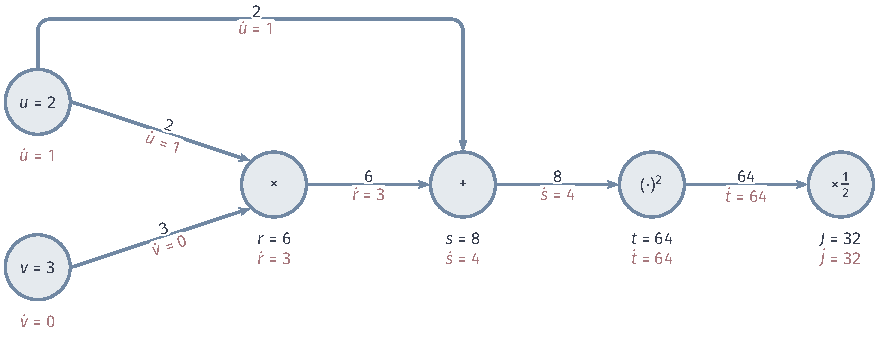
\includegraphics[width=148.791mm]{figures/05-neural-network-models/00-shared/tikz/ffn-autodiff-forward/figure.pdf}
  \caption{具体算子图上的前向模式。圆形节点表示乘法、加法、平方和缩放；实线上方的前向数字是传入算子的值，下方红色数字是同一路径上的方向导数。每个算子下方再用两行列出其输出值和输出方向导数。输入方向$(1,0)$给出$\partial J/\partial u=32$；加法处的$\dot s=3+1$包含了$u$的两条路径。}
  \label{fig:ffn-autodiff-forward}
\end{figure*}

图~\ref{fig:ffn-autodiff-forward}把一次方向导数计算附在原有算子图上。若要计算对$v$的偏导，改取$(\dot u,\dot v)=(0,1)$：此时$\dot r=2$、$\dot s=2$、$\dot t=32$，最终$\dot J=16$。两次遍历的前向值相同，变化的是输入方向以及随之传播的导数。

\FloatBarrier
\subsubsection{后向模式与梯度累加}
\label{sec:ffn-autodiff-reverse}

若希望从一个标量目标同时得到多个输入的导数，可以反过来问：输出对当前中间值有多敏感？\term{后向模式}（reverse mode）从输出向输入累积这种敏感度。记$\bar r=\partial J/\partial r$，对其他变量采用相同横线记号；前向值仍保留在原算子图中，从$\bar J=1$开始回传：
\begin{equation}
  \begin{aligned}
    \bar t&=\tfrac12\bar J,&\bar s&=2s\bar t,\\
    \bar r&=\bar s,&\bar u&=\bar r v+\bar s,\\
    &&\bar v&=\bar r u\text{。}
  \end{aligned}
  \label{eq:ffn-reverse-mode}
\end{equation}
每条回传贡献等于下游敏感度乘该条依赖的局部导数。缩放算子给出$\bar t=1/2$，平方算子利用保存的$s=8$得到$\bar s=8$，加法向两个输入各传递$8$。其中传给$r$的$8$再经过乘法，分别给$u$和$v$贡献$8v=24$与$8u=16$。

\begin{figure*}[htb]
  \centering
  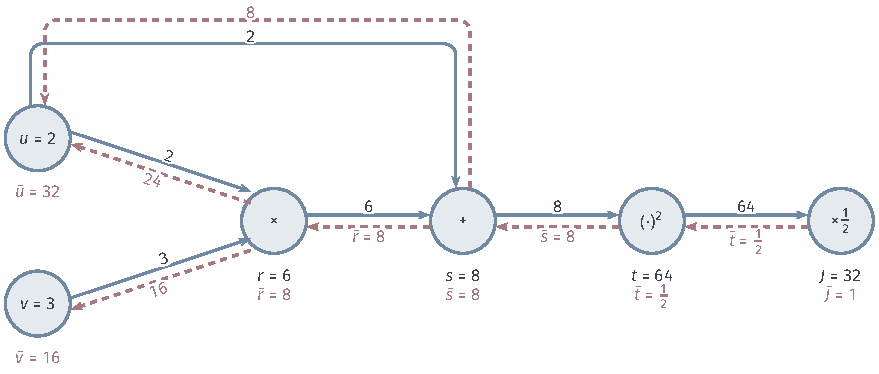
\includegraphics[width=148.791mm]{figures/05-neural-network-models/00-shared/tikz/ffn-autodiff-reverse/figure.pdf}
  \caption{同一算子图上的后向模式。节点位置与前向模式相同，实线及其前向标注保留前向传递值，红色虚线及其标注从$\bar J=1$开始回传导数贡献；每个算子下方两行分别给出输出值和伴随值。输入$u$收到经乘法传来的$24$和直接经加法传来的$8$，累加为$32$；输入$v$得到$16$。一次后向遍历同时得到两个偏导。}
  \label{fig:ffn-autodiff-reverse}
\end{figure*}

在图~\ref{fig:ffn-autodiff-reverse}中，$u$有两条通向目标的路径，所以$\bar u=24+8=32$。若漏掉直接进入加法的路径，就会错误地得到$24$。共享参数在多处被使用时也遵循同样规则：先保存各使用位置的局部回传贡献，再把它们累加到同一个参数。后向模式改变的是求导顺序，原函数的前向依赖并没有改变。

\FloatBarrier
\subsubsection{两种模式的计算代价}
\label{sec:ffn-autodiff-cost}

前面的算例有两个输入、一个输出。在$(u,v)=(2,3)$处，$J$的Jacobian矩阵是一行$(32,16)$：前向种子$(1,0)$取出第一列，前向种子$(0,1)$取出第二列；后向种子$\bar J=1$则把这一整行的转置作为输入梯度返回。一般映射可以有多个输出，这时后向模式也需要指定从哪些输出开始、各占多少权重。

对一般映射$\bm{F}:\mathbb{R}^{p}\to\mathbb{R}^{q}$，Jacobian矩阵$\bm{J}_{\bm{F}}\in\mathbb{R}^{q\times p}$的行对应输出坐标、列对应输入坐标，梯度采用列向量。前向模式在给定输入方向$\bm{v}\in\mathbb{R}^{p}$时计算$\bm{J}_{\bm{F}}\bm{v}$，后向模式在给定输出权重$\bm{u}\in\mathbb{R}^{q}$时计算$\bm{J}_{\bm{F}}^{\top}\bm{u}$。二者都可直接计算乘积，无需存储完整Jacobian矩阵。用逐坐标方向构造完整Jacobian矩阵时，前向模式需要$p$个方向，后向模式需要$q$个方向；实际代价还取决于批处理、稀疏结构和基本算子的实现。

把一般映射的输入写为$\bm\theta\in\mathbb R^p$，并固定一个与输入无关的输出权重$\bm u$。后向种子$\bm u$所指定的求导对象，是加权标量$\psi_{\bm u}(\bm\theta)=\bm u^{\top}\bm F(\bm\theta)$；对第$k$个输入坐标求导，有
\[
  \frac{\partial\psi_{\bm u}}{\partial\theta_k}
    =\sum_{i=1}^{q}u_i\frac{\partial F_i}{\partial\theta_k},
  \qquad
  \nabla_{\bm\theta}\psi_{\bm u}
    =\bm J_{\bm F}^{\top}\bm u\text{。}
\]
因此一次后向计算把各输出对输入的影响，按所选权重相加。取$\bm u$为第$i$个输出坐标的标准基向量，就只保留$F_i$，返回Jacobian第$i$行的转置。逐个选择全部$q$个输出坐标，才恢复全部行。

前向模式则把Jacobian的各列按输入方向的坐标加权，即
\[
  \bm J_{\bm F}\bm v=\sum_{k=1}^{p}v_k(\bm J_{\bm F})_{:,k}\text{。}
\]
取第$k$个输入标准基向量，就只保留第$k$列，逐个选择$p$个输入坐标才恢复全部列。前面标量算例正是$p=2$、$q=1$的情形；训练虽可输出多个类别得分，损失汇总后仍是一个标量，所以对参数求损失梯度只需一个后向种子$1$。

神经网络训练通常有很多参数，却只有一个标量目标，即$q=1$。后向模式从该目标出发，能够在与前向求值同阶的算术工作中得到完整参数梯度，代价是保存或重新计算反向所需的中间值。前述反向传播就是后向模式在神经网络损失上的具体应用\scite{baydin2018autodiff}

如果计算图包含多条损失分支，梯度在共同上游节点相加；如果某些分支被有意停止求导，它们就不再贡献上游梯度。离散采样、取整和按值选择分支也需要分别判断可微性：自动微分通常沿当前执行路径应用已登记的规则，不会自行补上对离散选择概率的导数。核验所得梯度时，需要同时检查目标、依赖路径和特殊算子的求导规则；数值梯度检查可进一步检验选定点附近的计算。

\section{前馈神经网络的扩展}
\label{sec:ffn-extensions}

前两节默认输入已经是一串数值。但真实数据里充满了\emph{类别信息}：设备型号、用户性别、语言中的词、商品编号。这些对象的共同特点是：它们用一个“编号”或“名字”标识身份，编号本身却不携带任何可以直接计算的数值含义——把“手机”编号成3并不意味着它是“平板（编号2）”的1.5倍。如果直接把编号当成一个实数喂给网络，模型就会被迫在编号的大小关系上做文章，而这种大小关系完全是人为随意指定的。

解决办法是把\emph{输入接口也纳入学习}：不让类别以一个编号数字进入，而是为每个类别学习一个简短的实数向量，让向量中各坐标的取值由任务数据决定；类别先经过这个可学习向量，再接入前面的前馈计算。这样，表示向量和后续预测参数就能由同一个任务共同调整。这一机制称为Embedding（嵌入），它不仅用于传统表格中的类别字段，也是现代语言模型处理词和符号的基础。

\subsection{支持高维离散表示：Embedding}
\label{sec:ffn-embedding}

考虑由设备类别和使用状态预测下一时间窗是否发生故障。使用时长等数值有单位和大小关系，设备类别的编号却只是身份标记。下面先用这项任务说明怎样为类别学习向量，再说明训练所得表示怎样预训练、迁移和部署使用。

\subsubsection{从高维稀疏表示到低维稠密表示}
\label{sec:ffn-embedding-motivation}

假设三个设备类别分别编号为$1,2,3$。若把编号直接作为一个实数送入线性单元，类别贡献就被写成$wc+b$，相邻编号之间的差别都由同一个$w$决定。重新给类别编号，还会改变这种数值关系。后续非线性网络可以学习更复杂的响应，但编号本身没有提供“类别2应处于类别1与类别3之间”的依据，因此不宜把身份编号的大小当成任务已知的规律。

一种不引入这种顺序的做法，是干脆不用一个数字、而是为每个类别单独分配一个坐标。编号为$c$的类别由向量$\bm{o}(c)$表示：第$c$个坐标为$1$，其他坐标为$0$。这就是\term{独热表示}（one-hot representation）。例如三个类别的向量分别为$(1,0,0)^{\top}$、$(0,1,0)^{\top}$和$(0,0,1)^{\top}$。它用“在哪个位置上为1”来表示身份，彻底去掉了编号之间的大小和顺序。其代价也很明显：任意两个不同类别之间的欧氏距离都等于$\sqrt{2}$，模型从表示本身得不到“哪两类更相近”的任何提示；哪些类别在当前任务中作用相近，必须由后续模型从数据中学习。

当类别很多时，独热向量的维度会随类别数增长。若直接接一个全连接层，每个类别还对应这一层的一整列权重。我们可以改为先给每个类别保存一个较短的可学习向量，让后续单元读取同一组向量坐标。这种把对象转成向量、供后续计算使用的表示称为\term{嵌入}（embedding）。这里具体学习的是类别身份到向量的映射，向量各坐标通常没有预先指定的名称，两个类别也可能得到相同向量。嵌入不是额外找回原始记录中的信息；它改变的是已知类别进入模型的参数化方式。

在类别数很大时，独热表示只有一个非零坐标，其余坐标都是零，因此是高维稀疏表示。本节关注嵌入宽度小于类别数的情形，将这种输入转换为较短的稠密向量：向量不再受“恰好一个坐标为$1$、其余为$0$”的限制，通常多个坐标同时取非零值。“稠密”并不要求每个坐标都非零，含有零坐标的向量也可以作为这类表示。这里的维度降低也不自动保证总参数更少，后面还需把嵌入表和后续投影一起计数。

\subsubsection{网络架构}
\label{sec:ffn-embedding-architecture}

设类别共有$K$个，类别编号$c\in\{1,\ldots,K\}$，嵌入宽度为$d_e$。用矩阵$\bm{E}\in\mathbb{R}^{K\times d_e}$保存参数，每一行存放一个类别的向量。为保持本章的列向量约定，取出第$c$行后将它转置，得到$\bm{e}_c\in\mathbb{R}^{d_e}$。这一操作也可以用独热向量写成
\begin{equation}
  \bm{e}_c=\bm{E}^{\top}\bm{o}(c),
  \qquad (\bm{e}_c)_k=E_{c,k},\quad k=1,\ldots,d_e\text{。}
  \label{eq:ffn-embedding-lookup}
\end{equation}
由于$\bm{o}(c)$只有一个非零坐标，乘法只选出对应的一行，并不需要真的生成长独热向量或执行完整稠密乘法。这种按编号读取参数向量的模块称为\term{嵌入层}（embedding layer）。单个编号的查表需要读取$d_e$个数，整张表仍需保存$Kd_e$个参数。独热输入上的线性映射与查表可以给出同一个结果，查表本身没有增加非线性。

回到故障预测，设$\bm{x}\in\mathbb{R}^{r}$记录预测时刻已经知道并按训练规则处理的数值变量。把它与$\bm{e}_c$拼接，便得到$r+d_e$维输入。一个含$m$个隐藏单元的二分类网络可以写为
\begin{equation}
  \begin{aligned}
    \bm{h}&=\sigma(\bm{W}_x\bm{x}+\bm{W}_e\bm{e}_c+\bm{b}),\\
    a&=\bm{w}_o^{\top}\bm{h}+b_o,\qquad p=s(a)\text{。}
  \end{aligned}
  \label{eq:ffn-embedding-classifier}
\end{equation}
其中$\bm{W}_x\in\mathbb{R}^{m\times r}$、$\bm{W}_e\in\mathbb{R}^{m\times d_e}$、$\bm{b},\bm{w}_o\in\mathbb{R}^{m}$，$b_o$为标量，$s$是前文的Sigmoid。$p$表示模型给出的故障概率。类别先决定查哪一行，取出的向量再与数值变量共同影响隐藏活动；整条前向路径没有环。多个类别字段可以分别设置嵌入表，再把各字段的向量与数值变量拼接，字段的含义和编号映射需要分别保存。

图~\ref{fig:ffn-embedding-architecture}把查表与后续网络接成一条前向路径。图中先放嵌入坐标、再放数值坐标，得到拼接向量$\bm{v}=[\bm{e}_c;\bm{x}]$；对应的全连接权重按$[\bm{W}_e\;\bm{W}_x]$排列，仍然得到式\eqref{eq:ffn-embedding-classifier}中的同一个加权和。两条输入路径在这里保留各自的坐标，拼接不等于把两个向量相加。

\begin{figure*}[htbp]
  \centering
  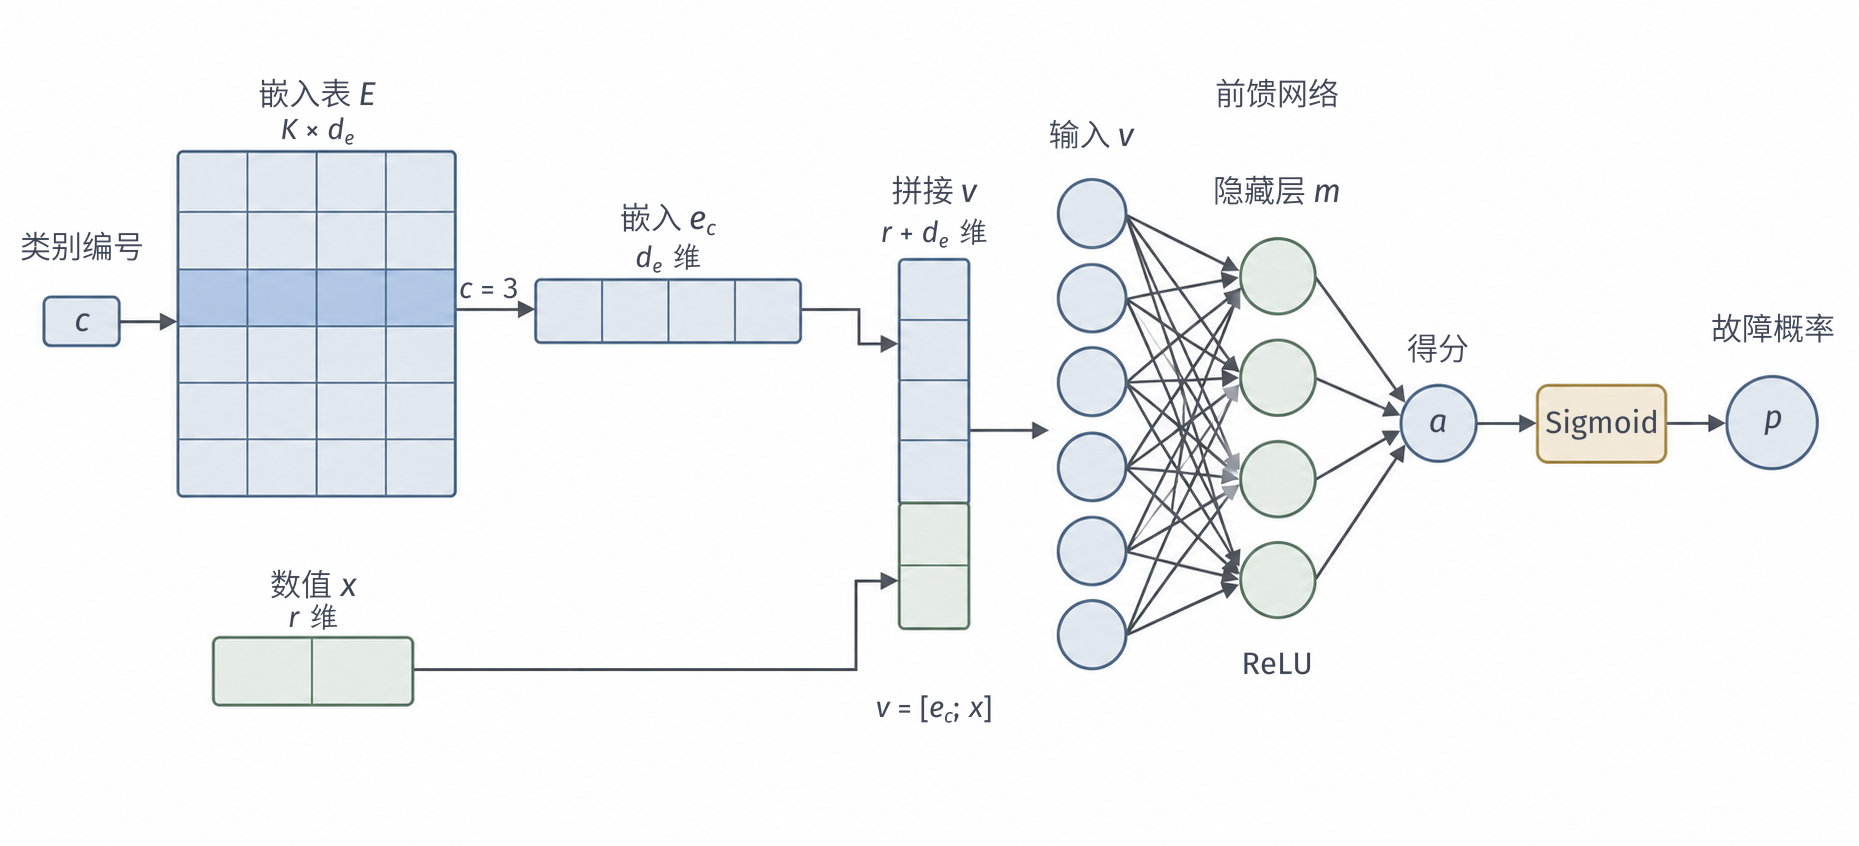
\includegraphics[width=169.000mm]{figures/05-neural-network-models/00-shared/generated/ffn-embedding-architecture/figure.png}
  \caption{嵌入层接入前馈二分类器的前向路径。教学示意取$K=6$、$d_e=4$、$r=2$、$m=4$，编号$c=3$选中嵌入表的第三行，读出四个嵌入坐标；横排的四格只表示坐标，数学运算仍采用列向量。蓝色嵌入与绿色数值特征按上四格、下两格拼接，右侧六个输入节点展开这六个坐标，经四个隐藏单元得到原始得分$a$，再经Sigmoid变成故障概率$p$。图只画前向计算，偏置未单独画出；格数和层宽是结构示意，不是训练实验。}
  \label{fig:ffn-embedding-architecture}
\end{figure*}
\FloatBarrier

较短向量引入了什么取舍，可以直接从第一层看出。若把独热向量直接送到同样宽度的隐藏层，类别部分需要一个$m\times K$矩阵。现在这部分变成$\bm{W}_e\bm{E}^{\top}$，参数数目由$mK$变为$Kd_e+md_e$，数值分支、偏置和输出层不参与这一比较。只有$d_e(K+m)<mK$时，这种分解才减少类别部分的参数；例如教学设定$K=100000$、$m=128$、$d_e=32$时，两者分别为$12800000$和$3204096$。查表避免生成独热向量，参数分解则在上述条件下减少存储，两项作用应分开判断。

这种分解也限制了类别到隐藏预激活的线性映射：$\bm{W}_e\bm{E}^{\top}$的秩至多为$d_e$，当$d_e<\min\{m,K\}$时，不能表达任意$m\times K$矩阵。不同类别仍有各自的一行参数，但后续计算共用$\bm{W}_e$对这$d_e$个坐标的解释。较小$d_e$可能提供适合任务的限制，也可能舍去任务需要的区别。因此，嵌入宽度是需要结合验证数据选择的超参数，不能由“使用了embedding”就推出表达更强、参数更少或预测更准确。

\FloatBarrier
\subsubsection{参数学习}
\label{sec:ffn-embedding-training}

向量的数值需要由数据确定。故障预测的一条训练记录为$(\bm{x}_i,c_i,y_i)$，其中$y_i\in\{0,1\}$说明指定时间窗内是否发生故障。用$\bm{\phi}$收集式\eqref{eq:ffn-embedding-classifier}中除嵌入表以外的网络参数，按前面的二元交叉熵比较预测与标签，可以共同学习$\bm{E}$和$\bm{\phi}$：
\begin{equation}
  \begin{aligned}
    \min_{\bm{E},\bm{\phi}}\quad &
    \frac{1}{n}\sum_{i=1}^{n}\ell(a_i,y_i)
    +\lambda\Omega(\bm{E},\bm{\phi}),\\
    \ell(a_i,y_i)&=\log(1+\exp(a_i))-y_i a_i\text{。}
  \end{aligned}
  \label{eq:ffn-embedding-objective}
\end{equation}
$a_i$由当前参数、$\bm{x}_i$和第$c_i$行嵌入计算得到，$\lambda\geq0$控制可选惩罚$\Omega$。这里奖励的是故障预测所需的表示，没有直接要求故障倾向相近的不同类别向量也具有较大的余弦相似度。不同坐标可以重新缩放，同时对下游权重作相反缩放而保持预测不变；这样的变化却可能改变向量夹角。因此，一个分类目标学到的嵌入不能自动解释成适合余弦检索的表示。

把这种缩放写成矩阵，可以区分统一倍乘与逐坐标改变尺度。令$\bm D$是对角元素均为正的可逆对角矩阵，把每个嵌入改为$\bm e'_c=\bm D\bm e_c$，同时把下游投影改为$\bm W'_e=\bm W_e\bm D^{-1}$。嵌入表相应变为$\bm E'=\bm E\bm D$，因为表中存放的是这些列向量的转置。于是$\bm W'_e\bm e'_c=\bm W_e\bm e_c$，其他参数不变时，隐藏预激活、预测概率和数据损失都保持不变。若不同坐标采用不同倍数，夹角却可能变化。例如$(1,1)^{\top}$与$(1,-1)^{\top}$原来的余弦为$0$；取$\bm D=\operatorname{diag}(2,1)$后，两向量变成$(2,1)^{\top}$与$(2,-1)^{\top}$，余弦为$(4-1)/(\sqrt5\sqrt5)=3/5$。这项等价只针对数据预测；参数惩罚$\Omega$可能随缩放改变，不能据此断言完整训练目标也不变。

反向传播怎样经过查表，可以从当前样本的损失开始。令$\bm{z}_i=\bm{W}_x\bm{x}_i+\bm{W}_e\bm{e}_{c_i}+\bm{b}$。在激活可微处，或采用前文约定的分段求导规则时，损失对嵌入向量的梯度为
\begin{equation}
  \bm{g}_i=\nabla_{\bm{e}_{c_i}}\ell
  =\bm{W}_e^{\top}\left[
    (p_i-y_i)\bm{w}_o\odot\sigma'(\bm{z}_i)
  \right]\in\mathbb{R}^{d_e}\text{。}
  \label{eq:ffn-embedding-vector-gradient}
\end{equation}
这仍是本章已经推导的链式法则：输出的$p_i-y_i$先传到隐藏层，再经过$\bm{W}_e$传到嵌入坐标。对表中元素$E_{c,k}$求导时，只有$c=c_i$才会经过这次读取，且该行第$k$项的局部导数为$1$。因此，小批量$B$的数据损失对整张表的梯度为
\begin{equation}
  \nabla_{\bm{E}}\frac{1}{|B|}\sum_{i\in B}\ell(a_i,y_i)
  =\frac{1}{|B|}\sum_{i\in B}\bm{o}(c_i)\bm{g}_i^{\top}\text{。}
  \label{eq:ffn-embedding-table-gradient}
\end{equation}
外积的形状为$K\times d_e$，每个样本把梯度放到自己读取的行；同一类别在批内多次出现时，贡献加到同一行。编号$c_i$是固定的离散选择，不需要对编号本身求导，待学习的是选中行的实数参数。这解释了为什么查表能够参加反向传播，而不是要求类别编号也连续可微。

\begin{example}[一次嵌入查表与更新]
  \label{ex:ffn-embedding-update}
  取三个设备类别、二维嵌入和两个ReLU隐藏单元，以下数值只是教学构造：
  \[
    \begin{aligned}
      \bm{E}&=\begin{pmatrix}1&0\\0&1\\1&1\end{pmatrix},
      &\bm{W}_x&=\begin{pmatrix}1\\-1\end{pmatrix},\\
      \bm{W}_e&=\bm{I}_2,
      &\bm{b}&=\bm{0},\\
      \bm{w}_o&=\begin{pmatrix}1\\-1\end{pmatrix},
      &b_o&=0\text{。}
    \end{aligned}
  \]
  令数值输入为$x=0.5$，类别为$c=3$，标签为$y=1$。查表得到$\bm{e}_3=(1,1)^{\top}$，因此$\bm{z}=(1.5,0.5)^{\top}$，两个ReLU都处于正半轴，$\bm{h}=\bm{z}$。输出为$a=1$、$p=s(1)\approx0.7311$，交叉熵约为$0.3133$。

  式\eqref{eq:ffn-embedding-vector-gradient}给出$\bm{g}\approx(-0.2689,0.2689)^{\top}$。若不加惩罚，学习率取$0.1$，普通梯度下降使第3行对应的列向量变为
  \[
    \bm{e}_3^{\mathrm{new}}
    =\bm{e}_3-0.1\bm{g}
    \approx(1.0269,0.9731)^{\top}\text{。}
  \]
  这一行的两个坐标沿不同方向调整，是因为当前输出用第一坐标减第二坐标来预测正类。前两行没有来自这次查表的数据梯度。这里单独展示表参数的变化；联合训练时，其余网络参数也按同一更新前参数计算梯度，再一起更新。
\end{example}

实际训练可以从适当尺度的随机嵌入表开始，其他层按前面与激活相配的规则初始化，然后沿算法~\ref{alg:ffn-minibatch-learning}执行查表、前向、反向和小批量更新，并按验证指标选择停止时刻与参数。若加入全表惩罚、使用带历史状态的优化器，或让这张表还参加输出计算，未在当前输入中查到的行也可能得到其他梯度或更新；上面“只进入选中行”的结论仅针对这次查表路径的数据梯度。少见类别的行得到的直接训练信号较少，单独保留一行参数也不能保证新类别有可靠表示。

\subsubsection{表达的使用}
\label{sec:ffn-embedding-use}

训练得到的嵌入首先要按训练时的接口使用。部署时需要连同参数保存类别到行号的映射和数值变量的转换规则：新记录先作相同预处理，再映射编号、查表、按式\eqref{eq:ffn-embedding-classifier}计算输出，分类任务按验证阶段确定的阈值决策。若重新排列类别编号却没有同步排列嵌入表，即使表内数值不变，也会把错误类别的向量交给网络。未见类别不能靠随机增加一行获得含义：可让多个未登记类别共用一个经过训练的未知项，舍去它们之间的区别；也可利用属性或文本描述经另一个表示网络计算向量，但这需要可获得的属性和相应训练依据。稀有类别得到的直接信号少，大表的存储仍按$Kd_e$增长，都要单独评价。

当前任务标签较少时，表示可以先在数据更多的其他目标上\emph{预训练}（pretraining）再迁移，但前提是两个任务共享可对应的输入：同一套设备编号可以复用对应行，词元表与设备编号之间没有行对应，就不能直接互换。一种不依赖人工类别的目标是词元预测：对固定窗口内的词元查表，接前馈网络用Softmax预测下一个词元，目标由文本自身构造，同一词元在不同窗口的梯度累加到同一行；这样学到的是服务于词元预测的表示，不自动适合故障分类或检索\scite{goodfellow2016}。若预期用途是检索，还需把“应当找回哪个对象”写进目标：设查询$\bm{u}$与$M$个候选文档向量$\bm{v}_j$均按式\eqref{eq:ffn-normalized-representation}归一化，以匹配文档为正确类，用温度$\tau>0$缩放余弦相似度后作候选Softmax，
\begin{equation}
  \ell_{\mathrm{pair}}
  =-\log\frac{\exp(\bm{u}^{\top}\bm{v}_1/\tau)}
  {\sum_{j=1}^{M}\exp(\bm{u}^{\top}\bm{v}_j/\tau)}\text{。}
  \label{eq:ffn-embedding-contrastive}
\end{equation}
这就是\term{对比学习}（contrastive learning）的一种形式：它沿用多类交叉熵，奖励匹配分数相对不匹配候选提高；若所有向量相同，损失为$\log M$，没有区分作用。负例选择和多个匹配文档的处理都要按任务规定；词元预测、故障分类与文档匹配给出的约束不同，学到的邻域关系也不必相同。这里的查询—文档训练组是教学构造，并非所引视觉对比方法的图像增强流程\scite{chen2020}

迁移到新任务时有两种参数选择。\emph{冻结}（freeze）表示保留嵌入表或编码器、只训练新任务的输出头，需要更新的参数少，但不能修正不合适的表示；\emph{微调}（fine-tuning）允许新任务损失继续更新表示，适应能力更强，但需要足够的当前数据支撑。两者都必须使用与预训练匹配的词表、切分、维度和预处理，并在当前任务的验证集上比较，不能只凭向量看起来成簇判断收益。检索场景还要先保存文档向量，查询到来时只编码查询、按约定的归一化与相似度排序返回；编码器或输入规则更新后，已保存的向量要重新计算，不同训练版本的同维向量不能仅凭维度相同混用。

最后区分查表向量与上下文表示。嵌入表对同一编号总返回同一向量，与它本次出现在什么句子中无关；要区分同一词在不同语境中的用法，后续网络必须读取上下文再计算表示。对多个词元取平均会丢失顺序，按固定位置拼接则保留窗口内的位置信息。因此embedding既可以是输入端的可学习查表，也可以是编码器输出的对象向量；其可用含义由输入、训练目标和实际使用方式共同决定。

\section{理论分析}
\label{sec:ffn-theory}

到目前为止，本章回答的都是“网络怎么算、怎么训”的操作性问题。本节退一步，回答三个决定这套方法是否可信的理论问题，它们恰好对应训练一个网络时最容易被混为一谈的三个阶段：
\begin{itemize}
  \item \emph{表达能力}：在所有可能的参数取值中，网络\textbf{能不能}表示（或足够逼近）我们想要的那个函数？这是“候选集合里有没有好答案”的问题，与训练无关。
  \item \emph{收敛性}：即使好参数确实存在，梯度下降\textbf{能不能}找到它，或者至少走到梯度足够小的点？这是“搜索算法找不找得到”的问题。
  \item \emph{泛化性}：即使在训练集上找到了损失很低的参数，它在没见过的新样本上\textbf{风险有多大}？这是“找到的答案能不能推广”的问题。
\end{itemize}
这三个问题需要分别判断，对其中一个的肯定回答不能代替另外两个：网络可以表达一切连续函数却难以优化，可以在训练集上损失为零却对新样本频频出错。下面三小节依次展开，并始终标明每个结论成立所需要的条件。

\subsection{表达能力}
\label{sec:ffn-expressivity}

先问最基本的存在性问题：给定一个想要学习的函数（比如一条复杂的非线性曲线），神经网络的参数空间里到底\emph{存不存在}一组参数能把它表示出来？前章的异或例子是一个精确表示结论：在指定的四个输入点上，确实存在一组参数使输出与标签完全一致。但真实输入通常是连续的，目标函数也往往不是四个离散点，这时更常见的问题是：能否让网络与目标函数\emph{足够接近}（误差小于任意给定的小正数$\varepsilon$），而不必逐点精确相等。\term{表达性}（expressivity）描述的就是网络族能够表示或逼近哪些函数；注意它的判断对象是\emph{整类}可选参数所形成的函数集合，而不是某次训练实际得到的那一个网络。

\begin{theorem}[前馈网络对紧集上连续目标的逼近能力]
\label{thm:ffn-continuous-approximation}
设$D\subset\mathbb R^d$为非空紧集，目标$g:D\to\mathbb R^q$连续。激活函数连续且不是多项式，网络允许隐藏偏置和线性输出。对任意$\varepsilon>0$，存在有限宽度的单隐藏层网络$f$，使
\[
 \sup_{\bm x\in D}\lVert f(\bm x)-g(\bm x)\rVert_2<\varepsilon\text{。}
\]
因此，对任意支撑在$D$上的输入分布$P_X$，同一候选满足
$\lVert f-g\rVert_{L^2(P_X)}<\varepsilon$。
\end{theorem}
标量情形见\BookChapterRef{chap:functional-analysis-and-approximation}{卷1《数学准备：计算、分析与几何》的“函数空间”章}；向量目标可逐坐标逼近：给每个坐标分配$\varepsilon/\sqrt q$的误差，把各标量网络的隐藏单元并列放入同一隐藏层、让第$j$个线性输出只读取自己那组单元，就得到有限宽度的向量网络。由于$P_X$是支撑在$D$上、总质量为一的概率测度，一致误差小于$\varepsilon$也控制$L^2(P_X)$平均误差。这里的宽度和参数可以随目标及精度改变，固定规模不享有任意精度保证；对分类问题可逐坐标逼近连续的条件概率函数，不连续目标或不受限输入域则需要另外分析。

通用逼近定理回答了“只要足够宽就能逼近”，但“宽”和“深”是两种不同的增加复杂度的方式：前者是在同一层并排更多单元，后者是把已有变换反复复合。要理解深度的独特作用，最好看一个函数，它用深网络表示很省、用浅网络表示却需要指数级数量的单元。

ReLU网络的一个直接读法是分段仿射变换。在一组隐藏单元的正负状态固定的输入区域内，每个ReLU都等价于原样保留某坐标或置零，整个网络因而是仿射的；不同的正负状态组合形成不同区域。有限个区域拼接起来就能近似弯曲形状，而一个固定大小的网络只有有限个这种区域。

一维情形能把这种拼接写成明确公式。设连续分段线性函数的内部转折点为$t_1<\cdots<t_m$，从左到右的斜率为$s_0,s_1,\ldots,s_m$，则可写成
\begin{equation}
  f(x)=c+s_0x+
  \sum_{j=1}^{m}(s_j-s_{j-1})\rho(x-t_j)\text{。}
  \label{eq:ffn-piecewise-linear-representation}
\end{equation}
每个ReLU项在对应转折点之后改变斜率，相邻段斜率在求和中逐项抵消，恰为当前段的$s_k$；$c$对齐整体高度，若网络没有直接的线性输入支路，可用$x=\rho(x)-\rho(-x)$补出$s_0x$。因此增加宽度就是增加可表达的转折。另一方面，紧区间上的连续函数由一致连续性，可取足够密的节点作线性插值，使节点间误差任意小；这条折线再由上式表示，就给出一维ReLU网络通用逼近的构造直觉。

深度提供另一种组织复杂函数的方式：重复复用已有变换。考虑$[0,1]$上的三角形函数
\begin{equation}
  T(x)=2\rho(x)-4\rho(x-1/2)+2\rho(x-1)\text{。}
  \label{eq:ffn-tent-function}
\end{equation}
它在$[0,1/2]$从$0$上升到$1$，在$[1/2,1]$再下降到$0$。令$T_k$表示$T$复合$k$次，而不是$T$的$k$次幂。每复合一次，每个线性区间又被分成两段，归纳可得$T_k$在$[0,1]$上有$2^k$个线性区间。

\begin{figure*}[htb]
  \centering
  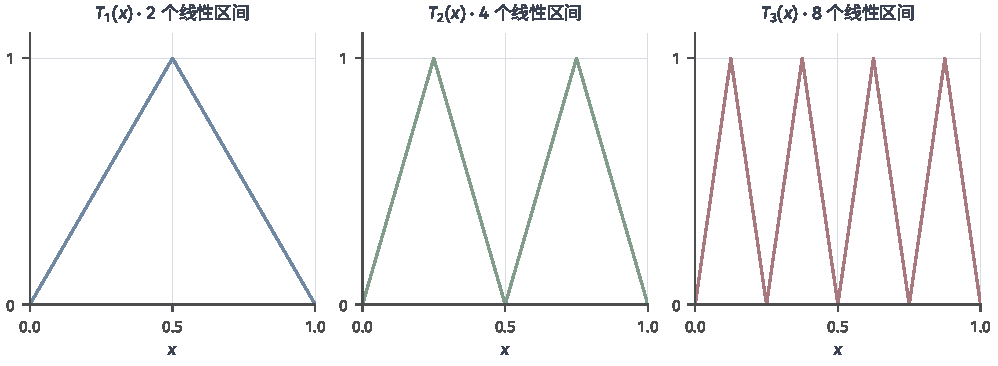
\includegraphics[width=159.059mm]{figures/05-neural-network-models/00-shared/matplotlib/ffn-depth-composition/figure.pdf}
  \caption{三角形函数的复合产生更多转折。三幅解析图分别为$T_1=T$、$T_2=T\circ T$和$T_3=T\circ T\circ T$，横轴均为$x\in[0,1]$，纵轴为函数值。每次复合将线性区间数翻倍；这是一维构造，不是实际训练实验，也不表示任意目标都能从增加深度中获得相同收益。}
  \label{fig:ffn-depth-composition}
\end{figure*}

这一复合可以落实为宽度固定的串联MLP：每个阶段只需三个隐藏单元读出$\rho(u)$、$\rho(u-\tfrac12)$、$\rho(u-1)$，再按系数$(2,-4,2)$线性组合并补上相应偏置，就得到下一阶段的输入$u$；重复$k$个这样的宽度为$3$的阶段、末端接线性读出即可，相邻阶段间的仿射映射可并入下一层权重。另一方面，$T_k$相邻段的斜率正负交替，$2^k$段之间确有$2^k-1$个不能合并的内部转折；而单隐藏层的一维ReLU网络中每个单元至多引入一个转折，精确表示$T_k$至少需要$2^k-1$个隐藏单元。图~\ref{fig:ffn-depth-composition}展示了这种重复组合的效率：深度随$k$线性增长、宽度保持常数，浅层表示却需要指数级单元。更一般的深度分离结果还需固定误差度量、目标函数族和比较网络的范围\scite{telgarsky2016depth}

这个例子固定同一个三角形复合目标，比较浅层与深层表示所需的单元数；训练难度和新样本风险是另外两个评价对象。某些目标用浅层结构已经足够；若目标本身具有可复用的组合规律，深度才可能以较少单元组织这种规律。表达能力的分析因此应同时说明目标、激活、深度、宽度和逼近精度。


\subsection{收敛性}
\label{sec:ffn-convergence}

隐藏层与输出层共同学习时，参数通过多层复合相互耦合，训练目标通常非凸。对于有下界、梯度为$\beta$-Lipschitz的光滑目标，完整梯度下降采用不超过$1/\beta$的固定正步长，可以使前若干步的平均平方梯度随步数增加而趋于零。这保证迭代中出现接近一阶驻点的位置，不能保证到达全局最优；ReLU拐点、小批量抽样和自适应更新还需各自的条件。相关优化结论可参考\BookChapterRef{chap:optimization}{卷1《数学准备：计算、分析与几何》的“最优化”章}。

固定隐藏表示、只学习带正二次惩罚的线性回归读出时，目标成为严格凸二次问题，具有唯一解；端到端训练通常不具备这份凸性。反向传播负责正确计算学习信号，优化器和停止规则怎样使用它，可参考本卷第\ref{chap:neural-network-training}章。

\subsection{泛化性}
\label{sec:ffn-learnability}

训练误差低还需要与有限样本的泛化保证一起判断。在独立同分布抽样、输入与损失满足相应尺度条件时，候选函数的复杂度或学习算法的稳定性可以控制训练风险与新样本期望风险的差距。对分类网络，参数范数还要与分类间隔一起考察；仅增加宽度或减小某一层权重，均不能单独保证预测更可靠。相关结论可参考\BookChapterRef{chap:deep-learning-theory}{卷3《基础、理论与可信性》的“深度学习的可学习性”章}。

合适的表示、充分且独立的样本，以及有效的训练共同决定新样本误差。训练与部署的分布不同，或多条记录来自同一对象而相互依赖时，还需按实际数据条件评价。本卷第\ref{chap:neural-network-generalization}章进一步说明数据增强、正则化和训练选择的作用。

\section{本章小结}
\label{sec:ffn-summary}

前馈神经网络把可学习表示落实为一条没有有向环的计算路径。全连接层组合已有坐标，非线性激活让多层复合超出仿射映射，输出变换与损失共同规定训练所要预测的对象。选择层宽和激活时，既要看能够形成怎样的函数，也要看参数量、计算量和梯度传播条件。

隐藏层的学习信号来自最终目标对它的敏感度。反向传播按链式法则逐层汇总这种影响，用局部导数和已有活动值计算所有参数梯度；自动微分将同样的原则推广到程序的实际计算路径。初始化决定起点，优化器使用梯度作出更新，二者都影响学习结果，正确求导只是完成训练的一个条件。

Embedding把输入表示也纳入这一学习过程：类别编号选取一行参数，下游损失决定该行怎样变化；更一般的编码器则根据输入计算对象向量。训练目标决定向量需要保留什么，部署时的编号、输入处理和比较规则决定这些向量能否被正确复用。

表达能力说明网络中是否存在合适的函数，优化分析说明训练能够找到怎样的参数，泛化结论则需要样本与学习条件。这些判断不能互相替代。前馈网络适合处理定长数值表示；具有空间、序列或关系结构的数据，还需要下一章起介绍的相应连接方式。

\paragraph{扩展阅读}
Goodfellow等教材第6章展开前馈网络与反向传播，计算图中的共享依赖解释了各梯度为何累加；第8章讨论所得梯度怎样用于优化，第7章讨论正则化如何限制候选和影响学习结果。这些内容分别对应本章的计算、求解与泛化问题\scite{goodfellow2016}

\chapter{卷积神经网络}
\label{chap:convolutional-networks}

先做一个思想实验：训练好一个能识别竖直边缘的全连接网络。它在图像左上角学会了“相邻像素左亮右暗”这一模式，靠的是连接到左上角那几个特定像素的权重。现在把同一条边缘平移到右下角——在把图像展平成一维向量后，右下角对应完全不同的几个坐标，也就是完全不同的一组权重，而这些权重并没有在左上角的样本中学过。于是网络很可能认不出右下角的这条边缘。要让它在每个位置都能识别，理论上必须让每种边缘在每个位置都出现足够多的训练样本，这显然代价高昂。

这个困难暴露了全连接结构处理图像的两个失配。其一，它把空间上相邻的像素和相距很远的像素同等对待，但判断“边缘”“拐角”这类局部模式，真正有用的信息几乎都来自邻近像素。其二，它让每个位置使用各自独立的权重，于是“在一处学会的规则”无法在结构上自动搬到另一处。然而图像数据恰好有两个鲜明特点：有意义的模式由邻近像素构成，而且同一种模式（一条边缘、一个色块）可能出现在画面任何位置。这就提出了本章的核心问题：\emph{怎样让网络保留空间结构，并让同一种识别规则在多个位置复用}？第~\ref{chap:feedforward-networks}章建立的多层非线性表示提供了基础，卷积神经网络则通过改变连接范围和权重复用方式来回答它。

卷积神经网络用同一组共享权重处理各个局部窗口，再由非线性激活和逐层组合，把局部的边缘、纹理逐级拼成部件乃至物体的预测。由于同一权重在前向计算中被反复使用，学习时就必须把所有位置传回的梯度汇集到这一个权重上；增加深度又改变了信息和梯度经过的路径，带来新的训练问题。本章的推进路线是：先精确定义卷积这一局部运算及其各种边界和采样约定（\ref{sec:cnn-convolution}节），再说明卷积层、池化层、归一化层如何组织成完整网络及经典架构（\ref{sec:cnn-structure}节），然后解决共享权重下的参数初始化与反向传播（\ref{sec:cnn-learning}节），接着介绍支持超深网络的跨层连接（\ref{sec:cnn-extensions}节），最后从理论上分析这种结构能表达什么、能否优化、泛化风险如何（\ref{sec:cnn-theory}节），并落到图像分割与生成等需要保留位置的任务上。激活函数、损失和链式法则沿用前章；结构约束与样本风险之间的统计联系可参考\BookChapterRef{chap:deep-learning-theory}{卷3《基础、理论与可信性》第8章“深度学习的可学习性”}。

\section{卷积神经网络概述}
\label{sec:cnn-overview}

先用一个具体数字看清全连接处理图像为何不可行。设一张彩色图像有$224\times224$个像素，每个像素包含红、绿、蓝三个颜色数值，展平后的输入维度为$224\times224\times3=150528$。若把它连接到$1024$个隐藏单元，仅这一层的权重就有$150528\times1024=154140672$个——还没有算偏置和后续各层。这个数字揭示了两个问题：一是参数量随输入像素数线性膨胀，极易过拟合并消耗巨大存储；二是这种稠密连接把每个输入坐标与每个隐藏单元相连，相邻像素和远隔像素被同等对待，每个位置还可以学到互不相干的局部规则，空间结构信息在展平的瞬间就丢失了。卷积要改变的，正是连接范围和权重复用这两件事。

针对图像的两个特点，可以分别施加两种结构约束。\term{局部感受野}（local receptive field）针对“模式由邻近像素构成”：让一个输出单元只读取输入中的一个小邻域（如$3\times3$窗口），把一次计算限定在附近的若干位置，而不与整张图相连。\term{参数共享}（parameter sharing）针对“同一模式出现在多处”：让图像上不同位置的输出单元使用\emph{同一组}权重，相当于把同一种局部识别规则（比如“检测竖直边缘”）像一把滑动的尺子一样重复应用到整张图像。二者回答不同的问题：局部连接决定一次计算\emph{读取哪里}，参数共享决定不同位置\emph{是否使用同一规则}；需要注意，只限制读取范围并不会自动带来共享——若不共享，各位置仍各自拥有一套权重。

\term{卷积神经网络}（convolutional neural network, CNN）就是把这种\emph{共享的局部计算}与非线性变换逐层堆叠起来，从数据中端到端地学习局部特征及其组合。这里需要引入“通道”这一组织方式。输入图像通常不止一个数值平面：彩色图像的红、绿、蓝就是三个\term{通道}（channel），每个通道是一张与图像等大的数值平面。在网络内部，每个空间位置会并列保存若干种不同的局部特征（如一个通道专门响应某种边缘），同一种特征在所有位置的响应合起来称为一张\term{特征图}（feature map）；一个输出通道就是“一种局部响应在所有输出位置上组成的数值平面”。因此普通密集卷积中，每种输出响应使用一组覆盖全部输入通道的权重，$64$个输出通道意味着$64$组不同的权重（对应$64$种被检测的局部模式），而不是$64$个空间位置。

参数共享带来的节省可以直接核算。对三个输入通道、$64$个输出通道的$3\times3$卷积层，每组权重在三个输入平面上各覆盖一个$3\times3$窗口，权重总数为$3\times3\times3\times64=1728$，再加每个输出通道一个偏置，共$64$个。这个数量只由核尺寸和通道数决定，与图像多大无关：图像变大后，同一组核只是在更多位置滑动，参数数保持不变。对比前面全连接层的一亿多个权重，差异来自两个方面——每个输出只看一个$3\times3$邻域（而非全部像素），且所有位置共用权重（而非各学一套）。需要说明，参数量少并不自动等于表达能力弱：全连接层输出一个隐藏向量，卷积层输出多张保留空间位置的特征图，二者的能力还取决于各自保留了什么信息以及后续如何组合。

共享局部规则还带来一种与“物体移动”有关的重要性质，初学时常与另一个概念混淆，这里先区分清楚。\term{平移等变性}（translation equivariance）指\emph{特征响应对位置保持同步}：输入中的图案移到哪里，输出特征图中的对应响应就移到哪里，相当于“检测结果跟着物体走”。\term{平移不变性}（translation invariance）则指\emph{最终输出不随平移改变}：物体移动后，网络给出的类别仍然相同。二者的差别在不同任务中至关重要：图像分类通常希望物体平移后类别不变（需要不变性），而图像分割必须让输出的轮廓随物体一起移动（需要等变性、不能丢弃位置）。步长为一的卷积在无限网格上天然与平移可交换（即具有等变性）；但在有限图像上，边界处理、下采样和最终的汇聚读出都会改变这一性质。要从“随位置移动的特征”得到“与位置无关的类别”，还需要池化等汇聚操作，具体条件见后文池化部分。

最后说明卷积的适用范围。这套结构假设数据具有三个性质：排列在\emph{规则网格}上、邻近位置\emph{局部相关}、同一种模式在不同位置\emph{重复出现}。图像是二维网格，音频波形和时间序列是一维网格，医学体数据是三维网格，都符合这些假设；序列任务还须限制只读取已发生的位置，避免“看到未来”。但如果输入的各个坐标只是含义不同的表格字段（年龄、收入、邮编……），交换相邻字段通常会改变含义，同一种局部规则也无法沿字段排列重复使用，这时卷积就不适用。是否采用卷积，取决于数据结构是否真的与这些假设相符。

局部处理与逐层汇聚的思想早于今天的大规模深度学习。Fukushima于1980年提出的Neocognitron交替组织局部模式检测与汇聚，使高层能够组合低层响应，并容忍一定的位置变化。它借鉴视觉系统的分层处理，但采用的学习机制与今天端到端反向传播的CNN不同；第~\ref{sec:neural-biological-system}节已介绍这条视觉启发线索\scite{fukushima1980}
到20世纪90年代，LeCun等将可学习卷积、降采样和梯度学习结合，用于手写字符和文档识别。1998年的LeNet-5展示了从像素到类别联合学习的完整系统：任务损失同时决定局部特征与后续分类。多层结构已进入实际识别系统，大规模视觉训练所需的数据和计算条件仍在发展\scite{lecun1998}

卷积结构解决了连接组织问题，深层网络能否有效训练仍是另一道关口。2006年，Hinton、Osindero和Teh提出深度信念网络的逐层学习方法：先学习一层隐表示，再把该表示作为下一层的训练数据，并对整个生成模型作后续微调。\term{逐层预训练}就是先分别为各层寻找有用的初始表示，减少从随机参数同时训练全部层的困难。这项工作为研究深层表示提供了可操作的训练途径，是理解随后深度学习兴起的一项重要进展。它研究的是生成式深层模型，原文的微调采用对比形式的wake--sleep算法，与后来判别式CNN的直接监督训练具有不同的目标和步骤\scite{hinton2006deepbelief}

\Needspace{14\baselineskip}
另一条路线继续探索直接用监督信号训练卷积网络。GPU能够并行执行大量规则乘加，使更宽、更深的模型获得实际可用的训练速度。Cireșan等在2011年报告了GPU上的可配置卷积网络，并在多个图像识别数据集上研究直接反向传播训练。这项工作把卷积训练的规则乘加交给GPU执行，为随后扩大模型和数据规模积累了实现经验\scite{ciresan2011cnn}
有标签数据集的扩大提供了更多视觉变化，GPU实现则让这些样本能够用于更大模型的迭代训练。结构、学习方法、数据与计算因而共同决定了当时可以实际训练的系统。

2012年，AlexNet在ImageNet大规模图像分类中将五个卷积层、ReLU、GPU训练、数据增强和全连接层中的Dropout组合起来，以监督学习从像素学习类别判别。论文报告的ILSVRC-2012参赛系统取得$15.3\%$的top-5测试错误率，第二名为$26.2\%$；这里的top-5错误指正确类别未进入前五个预测。$15.3\%$对应多个网络的组合，并包含额外ImageNet数据预训练；它衡量的是这套参赛系统，单个网络的误差另有报告。这个结果清楚展示了大规模学习特征相对于当时参赛方案的优势，推动卷积网络成为视觉研究的重要路线。这里的预训练是在更大标签集上的监督训练，与2006年的逐层生成式预训练不同\scite{krizhevsky2012}

此后的架构发展把问题进一步拆开：VGG用连续小核组织深度，GoogLeNet用多分支与通道压缩分配计算，Highway和ResNet为跨层信息提供路径，DenseNet让后层直接复用旧特征。它们将在本章相应小节中展开。把这段历史连起来，CNN的发展既包含“如何利用空间结构”的持续改进，也包含“如何让深层表示学得出来”的训练进展；深度学习的兴起是这些进展与数据、计算条件共同作用的结果。

\section{卷积运算}
\label{sec:cnn-convolution}

本节先把“卷积”这一步局部计算精确定义清楚。理解它的关键是抓住四个可以独立调节的“旋钮”：\textbf{核}决定每个局部窗口内各位置以多大权重组合；\textbf{边界规则}决定窗口滑出图像范围时读取什么；\textbf{步幅}决定相邻两个窗口相隔多远；\textbf{空洞率}决定窗口内部是密集采样还是跳过一些位置。此外还有一个看似奇怪、实则在图像生成中很常用的“反向”运算——转置卷积。本节逐一固定这些约定，再推广到多通道和不同实现。读者需要特别注意：深度学习里说的“卷积”通常省略了数学卷积中的核翻转，实际用的是互相关；这一区别下面会用算例讲清。数学卷积按固定核线性组合输入，并在相应边界下与平移交换（参考\BookSectionRef{sec:signal-analysis-lti-convolution}{卷1《数学准备：计算、分析与几何》第8章“信号”第8.3.3.1节“线性时不变条件下的卷积映射”}）。

\subsection{从数学卷积到网络运算}
\label{sec:cnn-convolution-definition}

卷积这个词来自信号处理，其核心直觉是“\emph{用一个小的权重模板（核）在输入上滑动，每到一处就计算模板与该处局部内容的匹配程度}”。数学卷积用\emph{相对位置}决定权重：对有限支撑的一维核$k$，离散输出为
\[
  y_i=\sum_a k_a x_{i-a}.
\]
本章的输入与核都是有限数组；输入在原矩阵以外如何取值要另行约定（补零或周期延拓），再通过裁剪决定保留哪些输出位置。

这里有一个初学者最容易困惑的细节：核的方向。二维核的数学卷积要同时反转行、列方向，相当于把核旋转$180$度后再滑动；而网络实现通常\emph{省去这次旋转}，直接按存储的核方向去匹配窗口，这种运算称为互相关。为什么要做这个区分？因为对一个需要学习的核来说，翻转与否只是把参数换了个排列位置，网络能学到的函数集合完全相同；但对一个预先给定、带特定方向含义的核，翻不翻转会改变结果。第~\ref{sec:cnn-matrix-operation}节会用同一个窗口并排比较这两种运算，让符号差异落到具体数值上。

固定核、完整网格及一致的边界约定下，输入平移会使输出同步平移。在线性系统分析中，这项性质称为平移不变性；描述网络的输入输出对应关系时，通常称为平移等变性。二者在此对应同一等式$L(T_rx)=T_r(Lx)$，含义都是输出随输入一起移动，只是两个领域的用语习惯不同。这一等式的成立是有条件的：有限图像上的边界、裁剪和跨步都会限制可用的平移范围；CNN还会学习核权重并在层间插入非线性，整个网络的输入输出关系因此超出了单纯的线性卷积。卷积核也可以含正、负权重，其尺度由学习目标和参数约束决定，不能把它理解成只能做平均的平滑模板。

\subsection{实际应用中的卷积}
\label{sec:cnn-practical-convolution}

\subsubsection{矩阵卷积：翻转与局部求和}
\label{sec:cnn-matrix-operation}

二维数据把单个位置扩展为行、列两个索引。本节采用从零开始的空间索引，输入矩阵为$\bm X\in\mathbb R^{h\times w}$，核为$\bm K\in\mathbb R^{k_h\times k_w}$，元素分别记为$x_{i,j}$和$k_{a,b}$。核索引$a,b$也从零开始。完整二维数学卷积写为
\begin{equation}
  y_{i,j}=\sum_{a=0}^{k_h-1}\sum_{b=0}^{k_w-1}
    k_{a,b}x_{i-a,j-b}\text{。}
  \label{eq:cnn-matrix-convolution}
\end{equation}
输入在原矩阵以外如何取值，需要另行约定。若只保留核完全落在输入内的位置，将输出重排成从零开始的索引，相当于先把核旋转$180$度，再在输入上滑动，对每个窗口作逐元素乘积和求和。

这里的重排需要区分原卷积坐标与窗口坐标。设$h\geq k_h$、$w\geq k_w$，原式中核完整落在输入内的输出坐标$(u,v)$满足$k_h-1\leq u\leq h-1$、$k_w-1\leq v\leq w-1$，因为最小的读取坐标分别为$u-(k_h-1)$和$v-(k_w-1)$。若改用窗口左上角$(i,j)$作为新坐标，原输出坐标就是$(i+k_h-1,j+k_w-1)$。将重新编号的输出记为$\bar y_{i,j}$，并在求和中换用$a'=k_h-1-a$、$b'=k_w-1-b$，便有
\[
  \begin{aligned}
    \bar y_{i,j}
      &=y_{i+k_h-1,j+k_w-1}\\
      &=\sum_{a'=0}^{k_h-1}\sum_{b'=0}^{k_w-1}
         k_{k_h-1-a',\,k_w-1-b'}x_{i+a',j+b'}\text{。}
  \end{aligned}
\]
此时$i=0,\ldots,h-k_h$、$j=0,\ldots,w-k_w$。输入索引随$a',b'$增大而向右下移动，核索引则沿两轴反向，这正是旋转核后再按窗口求和的来源。

用以下教学矩阵固定输入与权重：
\begin{equation}
  \bm X=\begin{bmatrix}
    1&2&3&4\\5&6&7&8\\9&10&11&12\\13&14&15&16
  \end{bmatrix},\qquad
  \bm K=\begin{bmatrix}1&0\\0&-1\end{bmatrix}\text{。}
  \label{eq:cnn-matrix-example}
\end{equation}
图~\ref{fig:cnn-kernel-flip}把同一窗口的两种运算并排比较。旋转后的核为$\left[\begin{smallmatrix}-1&0\\0&1\end{smallmatrix}\right]$，左上窗口给出$-1+6=5$。步长为一且不填充时，核有$3\times3$个合法位置，这里的每个数学卷积输出都是$5$。


本例$k_h=k_w=2$，所以重新编号后的左上输出$\bar y_{0,0}$对应原数学卷积的$y_{1,1}$。原式的$(0,0)$不属于核完整落在输入内的输出坐标；两种编号不能直接当成同一位置。

\begin{figure*}[htb]
  \centering
  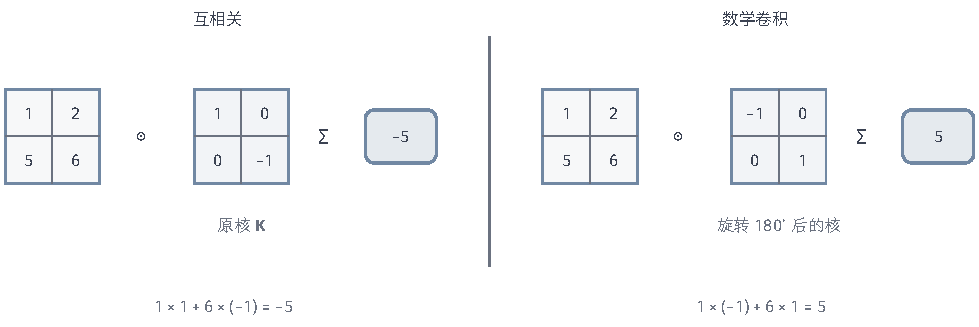
\includegraphics[width=165.767mm]{figures/05-neural-network-models/00-shared/tikz/cnn-kernel-flip/figure.pdf}
  \caption{核的方向改变输出。输入窗口固定为$\left[\begin{smallmatrix}1&2\\5&6\end{smallmatrix}\right]$，核固定为$\left[\begin{smallmatrix}1&0\\0&-1\end{smallmatrix}\right]$。左侧直接逐元素相乘后求和，得到互相关输出$-5$；右侧先把核旋转$180$度，再求和，得到数学卷积输出$5$。$\odot$表示逐元素乘法，$\sum$表示把四个乘积相加。}
  \label{fig:cnn-kernel-flip}
\end{figure*}
\subsubsection{互相关：保留核的方向}
\label{sec:cnn-correlation-operation}

网络通常省去这次旋转，直接用存储的核权重对窗口求和。这种\term{互相关}（cross-correlation）是按核原有方向匹配局部输入；本章针对实数数据写为
\begin{equation}
  y_{i,j}=\sum_{a=0}^{k_h-1}\sum_{b=0}^{k_w-1}
    k_{a,b}x_{i+a,j+b}\text{。}
  \label{eq:cnn-cross-correlation}
\end{equation}
于是左上窗口得到$1-6=-5$，全部输出构成$3\times3$的常数矩阵，见图~\ref{fig:cnn-sliding-window}。对无方向约束的可学习核，翻转只是参数位置的重新排列，卷积与互相关对应同一类候选映射；对预先给定的核，方向仍会改变结果。深度学习文献和软件通常把这种互相关也称为卷积。下文的网络公式遵循这一惯例，保留“数学卷积”来指明需要翻转的运算。

\begin{figure*}[htb]
  \centering
  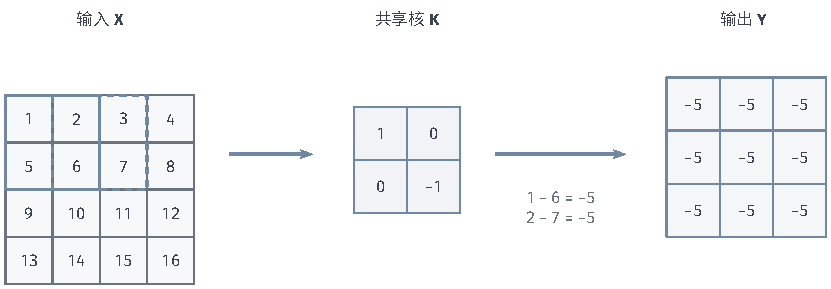
\includegraphics[width=140.723mm]{figures/05-neural-network-models/00-shared/tikz/cnn-sliding-window/figure.pdf}
  \caption{共享核在二维矩阵上滑动的教学例子。蓝色实线和虚线分别框出相邻的两个$2\times2$输入窗口，中间矩阵给出保持原方向的核，右侧矩阵给出互相关输出。每个输出计算窗口左上数值减去右下数值，因此均为$-5$；两个位置使用同一组权重。}
  \label{fig:cnn-sliding-window}
\end{figure*}

\subsubsection{数据填充：确定边界假设}
\label{sec:cnn-padding-operation}

如果不做任何处理，卷积会遇到两个边界问题。一是尺寸缩小：核必须完全落在图像内，$3\times3$核在$4\times4$图上只有$3\times3$个合法位置，每卷积一次特征图就变小一圈，深层网络很快缩没了。二是边缘像素被“轻视”：角落的像素只被一个窗口扫到，而内部像素被多个窗口反复读取，边缘信息参与计算的次数明显偏少。\term{数据填充}（padding）在矩阵外人为补充一圈数值，让核也能完整覆盖边缘附近的位置，从而解决这两个问题。补什么值则体现了对“图外是什么”的不同假设：零填充把外部值设为零；复制填充延续最近的边缘值；反射填充按边界镜像取值；循环填充把图像另一侧的数据接过来（适合本身具有周期性的信号）。这些外部值都是人为构造的，直接决定边缘窗口的计算结果，因此填充不是无关紧要的实现细节，而是一种边界假设。

对式\eqref{eq:cnn-matrix-example}只在右侧和下侧各补一列、一行零，输出就有$4\times4$个位置：
\begin{equation}
  \bm Y=\begin{bmatrix}
    -5&-5&-5&4\\-5&-5&-5&8\\-5&-5&-5&12\\13&14&15&16
  \end{bmatrix}\text{。}
  \label{eq:cnn-padding-example}
\end{equation}
最后一列和最后一行改变，是因为核的负权重落到了补零区域。图~\ref{fig:cnn-padding}标出右上和右下两个窗口：相同的核在内部读取真实数值，在边界则读取约定的零。\term{valid填充}表示不添加边界值，\term{same填充}通常表示按输入尺寸和步长选择填充，使输出尺寸达到约定值。步长为一时常取输出与输入等大；偶数核可能需要不对称填充，本例就是这种情况。步长大于一时，有些接口以$\lceil h/s_h\rceil$为目标高度，具体左右分配还需核对所用约定。


\begin{figure*}[htb]
  \centering
  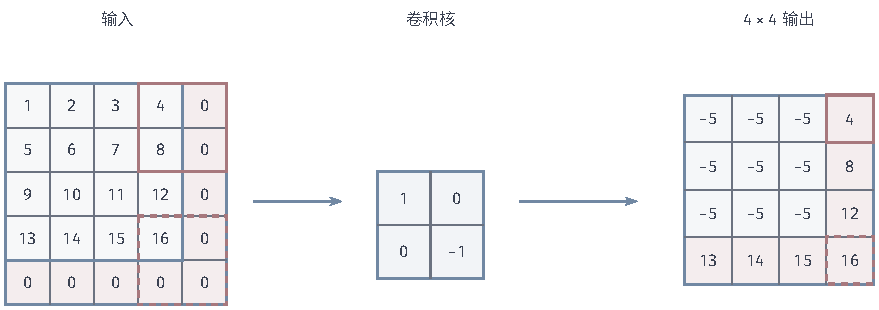
\includegraphics[width=148.791mm]{figures/05-neural-network-models/00-shared/tikz/cnn-padding/figure.pdf}
  \caption{不对称零填充与边界输出。蓝色框内是原$4\times4$输入，浅红色区域是右侧、下侧各新增的一列、一行零。红色实线窗口产生右上输出$4$，虚线窗口产生右下输出$16$，输出矩阵中用相同线型标记对应位置。核为$(1,0;0,-1)$，步长一、空洞率一，计算采用互相关。}
  \label{fig:cnn-padding}
\end{figure*}
\subsubsection{跨步卷积：改变窗口移动间隔}
\label{sec:cnn-stride-operation}

前面默认核每次只移动一格，输出与输入大致等大。有时我们希望\emph{在做局部变换的同时缩小特征图}，比如高层只需要粗略的空间布局、或要降低计算量。\term{跨步卷积}（strided convolution）让核每次沿高、宽分别跳过$s_h,s_w$个输入位置再计算下一个输出，从而直接减少输出位置的密度。在原例中，不填充且$s_h=s_w=2$，只保留窗口起点$(0,0),(0,2),(2,0),(2,2)$，得到$2\times2$的输出，数值仍均为$-5$。图~\ref{fig:cnn-stride}显示，跨步改变的是\emph{窗口起点之间的间隔}（减少了起点数量），窗口内部仍然读取相邻的四个元素，并没有改变核本身。它把“局部变换”和“下采样”合并在一步完成。需要留意其代价：若输入在被跳过的位置之间含有较快的空间变化，隔点采样可能把不同的变化混到一起甚至漏掉细节，这正是信号处理中的混叠问题。


\begin{figure*}[htb]
  \centering
  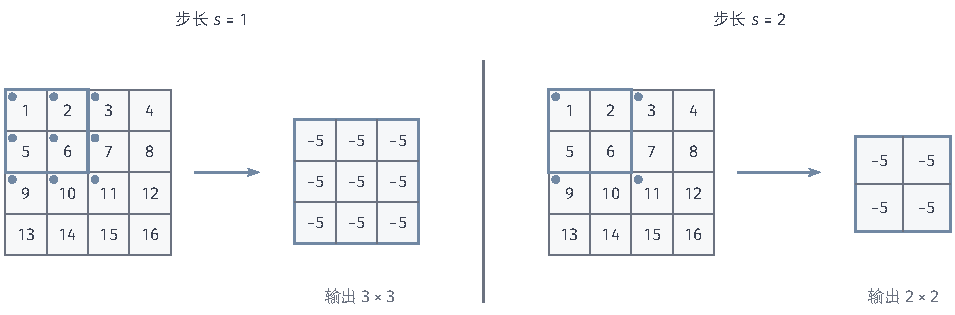
\includegraphics[width=161.766mm]{figures/05-neural-network-models/00-shared/tikz/cnn-stride/figure.pdf}
  \caption{跨步改变输出位置的密度。输入、$2\times2$核和无填充设置保持不变，只将高、宽步长从一改为二。每个蓝色圆点标记一个窗口的左上起点，起点分别形成$3\times3$和$2\times2$的网格；实线框只画出第一个窗口。该教学矩阵的所有窗口都得到$-5$，输出值相同不表示读取的位置相同。}
  \label{fig:cnn-stride}
\end{figure*}
\subsubsection{空洞卷积：改变核内采样间隔}
\label{sec:cnn-dilation-operation}

再考虑另一个需求：希望一个输出能\emph{看到}更大范围的上下文，却又不想增加核的参数量（加大核会带来更多权重和计算）。办法是保持核元素个数不变，但让它们在输入上\emph{隔开}采样。\term{空洞卷积}（dilated convolution）在相邻核元素之间跳过$d_h-1,d_w-1$个输入位置，$d_h,d_w$称为空洞率。原例取$d_h=d_w=2$、步长为一且不填充，左上输出变为$x_{0,0}-x_{2,2}=1-11=-10$，得到$2\times2$的常数输出。此时核仍只有四个权重，但它们覆盖了$3\times3$区域的四个角点而非紧密相邻的四格——\emph{感受野扩大了，参数量和计算量却没有增加}。图~\ref{fig:cnn-dilation}把权重与实际采样位置对应起来；图~\ref{fig:cnn-sampling}再并排区分“核内采样间隔”（空洞）与“窗口移动间隔”（步幅）这两个容易混淆的量。空洞卷积也有代价：重复使用相同空洞率可能在覆盖区域内留下始终读不到的网格位置，所以扩大覆盖范围不等于密集读取了其中所有信息。


\begin{figure*}[htb]
  \centering
  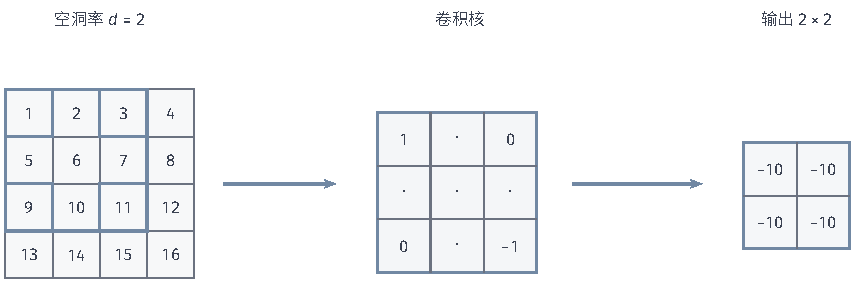
\includegraphics[width=144.766mm]{figures/05-neural-network-models/00-shared/tikz/cnn-dilation/figure.pdf}
  \caption{空洞率二时的实际采样位置。左图彩色小框标出左上输出读取的四格，蓝色外框标出其$3\times3$覆盖区域；中图把原$2\times2$核权重按采样间隔排开，点号表示跳过的位置。数值零占据一个已有核位置，点号处则没有核参数。步长一、无填充时，左上输出为$1-11=-10$，全部输出构成$2\times2$矩阵。}
  \label{fig:cnn-dilation}
\end{figure*}
\subsubsection{统一表达与输出尺寸}
\label{sec:cnn-shape-operation}

把这些设置合在一起，记上下填充为$p_{\mathrm t},p_{\mathrm b}$、左右填充为$p_{\mathrm l},p_{\mathrm r}$，以$\widetilde x_{i,j}$表示在原坐标外扩展的输入值。互相关计算为
\begin{equation}
  y_{i,j}=\sum_{a=0}^{k_h-1}\sum_{b=0}^{k_w-1}
    k_{a,b}\widetilde x_{is_h-p_{\mathrm t}+ad_h,\,
                         js_w-p_{\mathrm l}+bd_w}\text{。}
  \label{eq:cnn-general-correlation}
\end{equation}
有效核尺寸为$e_h=d_h(k_h-1)+1$、$e_w=d_w(k_w-1)+1$，要求填充后的输入至少容纳一个窗口。使用只保留完整窗口的取整规则时，输出尺寸为
\begin{equation}
  \begin{aligned}
    h'&=\left\lfloor\frac{h+p_{\mathrm t}+p_{\mathrm b}-e_h}{s_h}\right\rfloor+1,\\
    w'&=\left\lfloor\frac{w+p_{\mathrm l}+p_{\mathrm r}-e_w}{s_w}\right\rfloor+1\text{。}
  \end{aligned}
  \label{eq:cnn-output-size}
\end{equation}
分子表示窗口起点可以移动的总距离，除以步长后取整得到可移动的次数，再加上起始窗口。这也解释了为什么同样的输出大小可能来自不同的输入大小：不足一个步长的尾部会被舍去。

\begin{figure*}[htb]
  \centering
  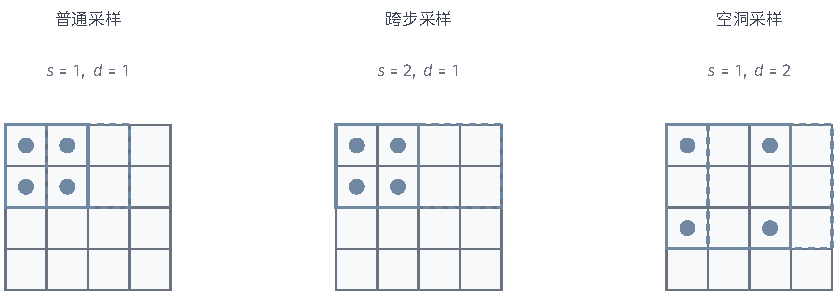
\includegraphics[width=141.792mm]{figures/05-neural-network-models/00-shared/tikz/cnn-sampling/figure.pdf}
  \caption{同一个$2\times2$核的三种采样设置。实线框给出一个输出所覆盖的区域，紫点是该窗口实际读取的位置，虚线框表示下一个水平窗口。普通设置与跨步设置的核内邻距均为一，后者将窗口起点移远；空洞设置将核内邻距增为二，窗口起点仍只移动一格。}
  \label{fig:cnn-sampling}
\end{figure*}

\subsubsection{转置卷积：把局部贡献分配回去}
\label{sec:cnn-transpose-operation}

转置卷积是初学者最容易误解的运算，需要先弄清它\emph{为什么会出现}，再看它做什么。普通卷积把一张较大的特征图压缩成较小的输出（尤其在步幅大于一时）；但在图像分割、生成这类任务中，网络往往需要\emph{反向地把分辨率放大}——从一个粗略的低分辨率特征图，恢复出逐像素的高分辨率输出。如何定义一个与卷积“方向相反”、能把一个输入值扩散到多个输出位置的可学习运算？这就是转置卷积的出发点。

先把普通卷积写成矩阵形式。固定核与输入、输出形状，把输入和输出展平为向量$\bm x$和$\bm y$，忽略偏置，则前向计算是一个线性映射$\bm y=\bm C\bm x$；矩阵$\bm C$的每一行对应一个输出，行中的非零位置标出它读取了哪些输入，共享权重在多行重复出现。\term{转置卷积}（transposed convolution）直接使用这个矩阵的转置：对给定的$\bm v$计算$\bm C^\top\bm v$。从作用上看，普通卷积是“把一个窗口内的多个输入\emph{汇聚}成一个输出”，转置卷积则反过来“把一个输入值按核权重\emph{分配}到多个输出位置”，并把不同输入分配到同一位置的贡献相加。

取原例第一行$(1,2,3,4)$，用一维核$(1,-1)$说明同样的过程。步长为一且不填充时，
\begin{equation}
  \bm C=\begin{bmatrix}
    1&-1&0&0\\0&1&-1&0\\0&0&1&-1
  \end{bmatrix},\qquad
  \bm C^\top\begin{bmatrix}1\\1\\1\end{bmatrix}
    =\begin{bmatrix}1\\0\\0\\-1\end{bmatrix}\text{。}
  \label{eq:cnn-transpose-example}
\end{equation}
图~\ref{fig:cnn-transpose-scatter}逐项展开分配过程。中间两个位置各收到正、负贡献，累加后成为零；转置映射的结果由这些贡献共同确定。这里必须澄清一个常见误解：\emph{转置卷积不是卷积的逆运算，不能把下采样丢掉的信息还原回来}。$\bm C$把四维输入压成三维输出，已经丢失了部分信息；而$\bm C^\top\bm C$一般不等于单位矩阵，所以$\bm C^\top$只是把贡献“铺回去”，铺回的结果由核权重决定，并非恢复原始输入。本例中它执行的是一次重新分配，前向已丢失的信息仍然没有恢复。作为网络中的可学习层时，转置卷积也可以独立学习自己的核参数，与对应前向卷积的核不必相同。


\begin{figure}[htb]
  \centering
  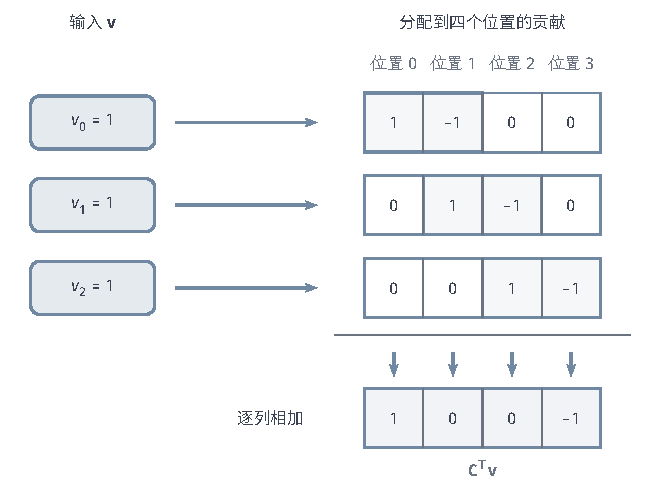
\includegraphics[width=112.000mm]{figures/05-neural-network-models/00-shared/tikz/cnn-transpose-scatter/figure.pdf}
  \caption{转置卷积的分配与累加。输入为$\bm v=(1,1,1)^\top$，核为$(1,-1)$，步长一、无填充。每行分别表示一个输入值对四个输出位置的贡献，紫框圈出两个可能非零的位置；没有贡献的格子记为零。逐列相加得到$(1,0,0,-1)^\top$，中间两格均包含来自不同输入的重叠贡献。}
  \label{fig:cnn-transpose-scatter}
\end{figure}
\FloatBarrier
转置映射的目标长度为何还需要额外选择，可以从普通卷积的取整公式反解。设原输入长度为正整数$n$，对称零填充为非负整数$p$，步长$s$、空洞率$d$和核长$k$均为正整数，有效核长度为$e=d(k-1)+1$。在$n+2p\geq e$、至少容纳一个完整窗口时，普通卷积输出长度为$n'=\lfloor(n+2p-e)/s\rfloor+1$。固定这个正整数$n'$后，向下取整的定义给出
\[
  n'-1\leq\frac{n+2p-e}{s}<n'
  \quad\Longleftrightarrow\quad
  (n'-1)s\leq n+2p-e<n's\text{。}
\]
因此，令$o=n+2p-e-(n'-1)s$，就得到整数余量$0\leq o<s$；它记录最后一个完整窗口之后不足一步的剩余长度。把这一等式解出$n$，并将原输入长度作为转置映射的目标长度，就得到下面的尺寸表达式。反解时仍只接受正的目标长度，并保留上述完整窗口条件。

在一维对称零填充$p$、步长$s$、空洞率$d$和核长$k$的约定下，转置卷积输入长度$n'$对应的输出长度常写为
\begin{equation}
  n_{\mathrm{out}}=(n'-1)s-2p+d(k-1)+1+o,
  \qquad 0\leq o<s\text{。}
  \label{eq:cnn-transposed-size}
\end{equation}
这里$o$是用于选择目标形状的输出填充量：普通卷积取整后，同一个$n'$可能对应$s$种原输入长度。选定目标长度后，前向矩阵的列数及其转置的输出形状才随之确定。$o$是尺寸约定，不表示把$o$个零作为最终输出值附在末尾。二维情形沿高、宽分别使用该式。不对称填充或额外裁剪会改变矩阵的边界行、列，输出形状也要随对应映射确定。跨步转置卷积可理解为先在输入位置之间插零，再进行适当的滤波与裁剪；不同位置的覆盖次数可能不均匀，需要检查输出中的周期性纹理。卷积尺寸与转置关系的系统说明见Dumoulin和Visin的算术指南\scite{dumoulin2016arithmetic}

例如取$k=3$、$d=1$、$s=2$、$p=0$，长度$n=5$与$n=6$都给出$n'=2$：相应计算分别为$\lfloor(5-3)/2\rfloor+1=2$和$\lfloor(6-3)/2\rfloor+1=2$。反解得到$n_{\mathrm{out}}=5+o$，选择$o=0$与$o=1$就分别确定五维和六维目标。两个前向矩阵都有两行，但分别有五列和六列；因此，它们的转置虽然都接收两个数，却输出不同长度的向量。$o$确定的是采用哪一种形状的映射，具体输出值仍由对应矩阵的转置计算。

覆盖不均也可以用一个跨步分配例子直接检查。取三个输入值均为一，核为$(1,1,1)$，步长二、无填充、空洞率一，并取$o=0$，则转置输出长度为七。三个输入分别向位置$\{0,1,2\}$、$\{2,3,4\}$和$\{4,5,6\}$分配贡献，逐位置累加得到$(1,1,2,1,2,1,1)$。中间位置收到的贡献次数交替为一、二，即使输入与核值相同，输出也会出现强弱交替；一般输入和权重还会改变这些贡献的数值。

\subsection{卷积的实现}
\label{sec:cnn-implementation}

固定边界与采样设置，在精确算术下，直接求和、矩阵化和满足适用条件的变换算法可以得到相同的预激活值。矩阵化汇集原有局部点积，Toom--Cook、Winograd与FFT通过变换输入和核来重组乘积，空间可分离路线则利用核的低秩结构（代数算法、数值例子及误差条件参考\BookSectionRef{sec:signal-analysis-fast-transforms}{卷1《数学准备：计算、分析与几何》第8章“信号”第8.4节“卷积映射的快速计算”}）。这里固定本层的批量、通道和采样设置，比较直接计算的成本与变换结果的复用，再说明数据如何存储和读取。

此前的单矩阵例子只保留一个数值平面，现在将第~\ref{sec:cnn-overview}节的多通道组织写成张量。一个通道在全部空间位置上的响应构成一张\term{特征图}（feature map）。单个输入的形状为$\bm X\in\mathbb R^{h\times w\times c_{\mathrm{in}}}$，普通密集卷积的核张量为$\bm W\in\mathbb R^{k_h\times k_w\times c_{\mathrm{in}}\times c_{\mathrm{out}}}$。固定一个输出通道，其核覆盖全部输入通道：对空间窗口和输入通道共同求和，产生一个输出值；换用另一组核权重便产生另一个输出通道。因此输入通道轴参与求和，输出通道轴保留在结果中，图~\ref{fig:cnn-channels}给出了对应示意。

以下比较同一个互相关映射，忽略激活；偏置可在累积完成后加入。设小批量含$n_{\mathrm b}$个输入，输入、输出通道数为$c_{\mathrm{in}},c_{\mathrm{out}}$，输出空间尺寸为$h'\times w'$。记
\[
  q=k_hk_wc_{\mathrm{in}},\qquad m=n_{\mathrm b}h'w'\text{，}
\]
即一个窗口的元素数与全部输出位置数。普通密集卷积需要$c_{\mathrm{out}}qm$次乘加；比较额外存储时，输入、核和最终输出不计入工作区。这里把输入数值与核权重相乘称为\emph{核心乘法}；在变换路线中，相应计数的是变换后输入与核的乘积。固定变换中的加减与常数乘法另外计算。总耗时还包含变换、数据读写与调度，后文据此同时计算新增的工作和存储。

矩阵化把本层的每个窗口作为一列，每个核作为一行。按一致顺序展平后，窗口矩阵为$\bm P\in\mathbb R^{q\times m}$，核矩阵为$\bm W_{\mathrm{loc}}\in\mathbb R^{c_{\mathrm{out}}\times q}$；加入偏置$\bm b\in\mathbb R^{c_{\mathrm{out}}}$后，预激活为
\begin{equation}
 \bm Z_{\mathrm{col}}=\bm W_{\mathrm{loc}}\bm P+\bm b\bm1_m^\top.
 \label{eq:cnn-im2col}
\end{equation}
其中$\bm1_m$是$m$维全一向量。这个矩阵等式把同一组局部点积汇集为\term{通用矩阵乘法}（general matrix multiplication, GEMM）；按普通矩阵乘法逐项求和时，乘加量仍与直接计算相同。

\subsubsection{直接计算：逐项求和}
\label{sec:cnn-direct-implementation}

直接算法在每个输出位置逐项累积窗口中的贡献。将批量索引记为$t$，输入元素为$x_{t,i,j,c}$，$w_{a,b,c,o}$表示核位置$(a,b)$上从输入通道$c$到输出通道$o$的权重。记$u(i,a)=is_h-p_{\mathrm t}+ad_h$、$v(j,b)=js_w-p_{\mathrm l}+bd_w$，即式\eqref{eq:cnn-general-correlation}中的实际读取位置，零填充下的核心步骤如下。
\Needspace{13\baselineskip}
\begin{algorithm}[直接多通道互相关]
  \label{alg:cnn-direct}
  \begin{algorithmic}[1]
    \Require 输入$\bm X$、核$\bm W$、偏置$\bm b$及形状、采样设置
    \Ensure 输出预激活$\bm Z$
    \For{每个合法的$(t,i,j,o)$}
      \State $z_{t,i,j,o}\gets b_o$
      \For{每个核位置$(a,b)$和输入通道$c$}
        \State 读取扩展输入$\widetilde x_{t,u(i,a),v(j,b),c}$
        \State $z_{t,i,j,o}\gets z_{t,i,j,o}+w_{a,b,c,o}\widetilde x_{t,u(i,a),v(j,b),c}$
      \EndFor
    \EndFor
  \end{algorithmic}
\end{algorithm}

算法\ref{alg:cnn-direct}的一次外层迭代只负责一个输出。核位置确定空间偏移，输入通道决定读取哪个数值，输出通道决定使用哪组权重；所有贡献加到同一个累积器中，完成后才写出。相邻输出重新使用核，另一个输出通道则使用另一个核，但二者都从同一输入张量取数。

对式\eqref{eq:cnn-matrix-example}的左上输出，顺序计算的四项是$1\times1$、$2\times0$、$5\times0$和$6\times(-1)$，总和为$-5$。零权重是这个例子的特殊取值，普通密集算法仍按四个位置组织计算；只有专门利用零权重结构，才能省去相应乘法。每个窗口含$q$项，一共有$c_{\mathrm{out}}m$个输出，因此乘加量为
\begin{equation}
  O\!\left(n_{\mathrm b}h'w'c_{\mathrm{in}}c_{\mathrm{out}}k_hk_w\right)\text{。}
  \label{eq:cnn-direct-cost}
\end{equation}
直接算法逐项保留局部求和结构，额外工作区可以只包含若干累积器，但算术量随核面积、通道数与输出位置数相乘。相邻窗口存在重叠时，共用输入可以在较近的存储中复用；这种复用属于第~\ref{sec:cnn-engineering}节的数据调度问题。判断一种计算算法时，应先固定数学运算及其乘加量，再考察它在具体存储层次中的执行方式。

\subsubsection{多通道卷积的变换复用}
\label{sec:cnn-transform-reuse}

本层的多个输出通道读取相同的窗口，同一个核又作用于多个位置。这两种共享关系使输入变换能跨输出通道复用，核变换能跨位置复用。
以步长一、无空洞的$3\times3$核为例，Winograd方案用固定矩阵$\bm B^\top,\bm G,\bm A^\top$分别变换输入、变换核并恢复输出，将一个$4\times4$输入块变为$2\times2$输出。其中输入变换矩阵为四行四列，核变换矩阵为四行三列，输出恢复矩阵为两行四列（变换矩阵及恢复等式参考\BookSectionRef{sec:signal-analysis-fast-winograd}{卷1《数学准备：计算、分析与几何》第8章“信号”第8.4.4节“基于余数分解的卷积计算”}）。
固定一个样本的输入块，对输入通道$c$和输出通道$o$，分别形成核变换$\bm U_{c,o}=\bm G\bm W_{c,o}\bm G^\top$与输入变换$\bm V_c=\bm B^\top\bm X_c\bm B$。其中$\bm W_{c,o}\in\mathbb R^{3\times3}$是核在通道$(c,o)$上的空间切片，$\bm X_c\in\mathbb R^{4\times4}$是该输入块在通道$c$上的空间切片。
通道累积与输出恢复写成
\begin{equation}
 \bm Y_o=\bm A^\top\left(\sum_c\bm U_{c,o}\odot\bm V_c\right)\bm A.
 \label{eq:cnn-winograd-channel-reuse}
\end{equation}
式中的乘积按对应位置逐元素相乘，再对全部输入通道求和。输入变换可供多个输出通道复用，核变换可供多个空间块与批量样本复用。
由于输出变换是线性的，先对通道求和再恢复，与逐通道恢复后相加等价，却只需为每个输出通道执行一次恢复。
若同时处理$n_{\mathrm{tile}}$个输入块，在每个变换位置上还可把核组合排成$c_{\mathrm{out}}\times c_{\mathrm{in}}$矩阵，输入组合排成$c_{\mathrm{in}}\times n_{\mathrm{tile}}$矩阵。
这一$F(2\times2,3\times3)$方案的记号依次表示输出块和核的空间尺寸。其变换结果可以组织为十六组通道矩阵乘法，与GEMM组合使用。

实现时将输出切为不重叠的$2\times2$块，各自读取$4\times4$输入块，再恢复四个空间输出并加偏置。
相邻输出块起点相隔两格，输入块重叠两行或两列；边缘不足一块时需要填充或单独处理。
变换核保存十六个系数，而原核只有九个系数，活动值工作区也会扩大；分块可以限制同时保存的变换值。
更大的输出块通常还会增加变换成本和数值敏感性，步长与空洞率改变后也不能直接沿用这些矩阵。

频域路线有相同的通道共享关系。对适当翻转并补零后的核，每个频率上的输出为$\widehat y_o=\sum_c\widehat x_c\widehat k_{c,o}$，随后对各输出通道反变换，并按本层规则裁剪和选取输出位置。
若补零后的二维网格含$N$个位置，核心频域乘加量为$O(n_{\mathrm b}c_{\mathrm{in}}c_{\mathrm{out}}N)$；输入、核和输出的变换成本分别为
\begin{align*}
 \text{输入变换：}\quad &O(n_{\mathrm b}c_{\mathrm{in}}N\log N),\\
 \text{核变换：}\quad &O(c_{\mathrm{in}}c_{\mathrm{out}}N\log N),\\
 \text{输出变换：}\quad &O(n_{\mathrm b}c_{\mathrm{out}}N\log N).
\end{align*}
这里$N$是二维网格的总位置数，复数乘法也不能按一次实数乘法计价。
输入频谱可供多个输出核复用，核频谱在参数不变时可跨样本复用；训练更新参数后需要重算。
Mathieu等研究了在CNN中利用这些复用关系的FFT实现\scite{mathieu2014fft}

将单个空间核分解为若干秩一核，可把二维滤波组织为若干组一维滤波，再将结果求和（分解与计算成本参考\BookSectionRef{sec:signal-analysis-fast-separable}{卷1《数学准备：计算、分析与几何》第8章“信号”第8.4.5节“基于核分离的卷积计算”}）。保留全部非零秩一项时，在相同边界和采样约定下恢复原来的空间核；计算能否减少，还取决于核的秩、输入尺寸与边界处理成本。截断分解会改变本层输出，需要检查近似误差或重新训练。第~\ref{sec:cnn-layer}节的深度可分离卷积则改变通道连接方式，以逐通道空间滤波和逐点通道混合两步构造新的参数结构。

\subsubsection{工程实现与优化}
\label{sec:cnn-engineering}

计算算法确定需要哪些乘积与求和，执行速度还取决于数据如何送入计算单元。\term{分块}（tiling）把相邻输出位置和若干通道放在一起计算，在较近的存储中复用它们共用的输入与核，减少重复读取。块越大，复用机会越多，但寄存器和局部存储需求也越高，可能限制并行度。

矩阵化卷积需要决定如何提供式\eqref{eq:cnn-im2col}中的窗口矩阵。\term{数据展开}（im2col）把窗口复制为连续的列，再调用GEMM；显式保存整个矩阵需要$qm$个元素，还会产生展开读写。\term{隐式GEMM}（implicit GEMM）则从原张量按需形成当前计算块所需的片段，省去完整展开矩阵，代价是加载时的地址计算与边界判断。CUTLASS给出了这种实现方式\scite{nvidiaCutlassConvolution}

另一种选择是\term{间接卷积}（indirect convolution）：保存指向原输入通道向量的地址，由专用内核沿地址取数，避免复制全部窗口数值。它与隐式GEMM的区别在于显式记录取数位置，也需要承担地址表和间接访存的成本；沿地址取数需要专门的执行内核，普通GEMM接收的则是数值矩阵\scite{dukhan2019indirect}

卷积之后的偏置和逐元素激活还可在写出前完成，这种\term{算子融合}（operator fusion）减少中间结果的读写与调用次数。分块、布局和融合可用于不同算法，但收益取决于层形状、精度、硬件及训练或推理条件。完整算子的时间、工作区与数值误差，反映了乘法节省与新增成本的合计结果。存储层次、并行调度与融合的具体实现留到
\BookVolumeRef{vol:systems}{卷12《系统》}展开。

\FloatBarrier

\section{网络结构}
\label{sec:cnn-structure}

理解了单个卷积运算之后，本节把这些运算组装成能完成任务的完整网络。一次局部求和只能产生一组线性响应，而且只对应一种局部模式；要识别多种特征、引入非线性、逐步扩大视野并最终给出可比较的预测，还需要不同类型的层各司其职。下面依次说明卷积层（用多个核并行提取多种局部特征及其通道变体）、池化层（汇聚并压缩空间）、激活与归一化层（引入非线性并稳定训练）、以及面向不同任务的输出头，最后把它们组合成LeNet到GoogLeNet等经典架构，看清每种设计在解决什么具体问题。

\subsection{卷积层}
\label{sec:cnn-layer}

沿用第~\ref{sec:cnn-implementation}节的输入与核张量形状，加入偏置$\bm b\in\mathbb R^{c_{\mathrm{out}}}$。空间和核索引从零开始，通道索引$c,o$从一开始；$x_{i,j,c}$、$w_{a,b,c,o}$、$b_o$分别是输入、核与偏置的元素。输出预激活值$\bm Z\in\mathbb R^{h'\times w'\times c_{\mathrm{out}}}$为
\begin{equation}
  \begin{aligned}
    z_{i,j,o}=b_o+\sum_{c=1}^{c_{\mathrm{in}}}
      \sum_{a=0}^{k_h-1}\sum_{b=0}^{k_w-1}
      w_{a,b,c,o}\widetilde x_{u(i,a),v(j,b),c},\\
    u(i,a)=is_h-p_{\mathrm t}+ad_h,\qquad
    v(j,b)=js_w-p_{\mathrm l}+bd_w\text{。}
  \end{aligned}
  \label{eq:cnn-layer-forward}
\end{equation}
随后通常逐元素应用激活，得到$h_{i,j,o}=\sigma(z_{i,j,o})$。图~\ref{fig:cnn-channels}把式中的通道求和展开，展示同一组输入怎样形成多个输出通道。

\begin{figure*}[htb]
  \centering
  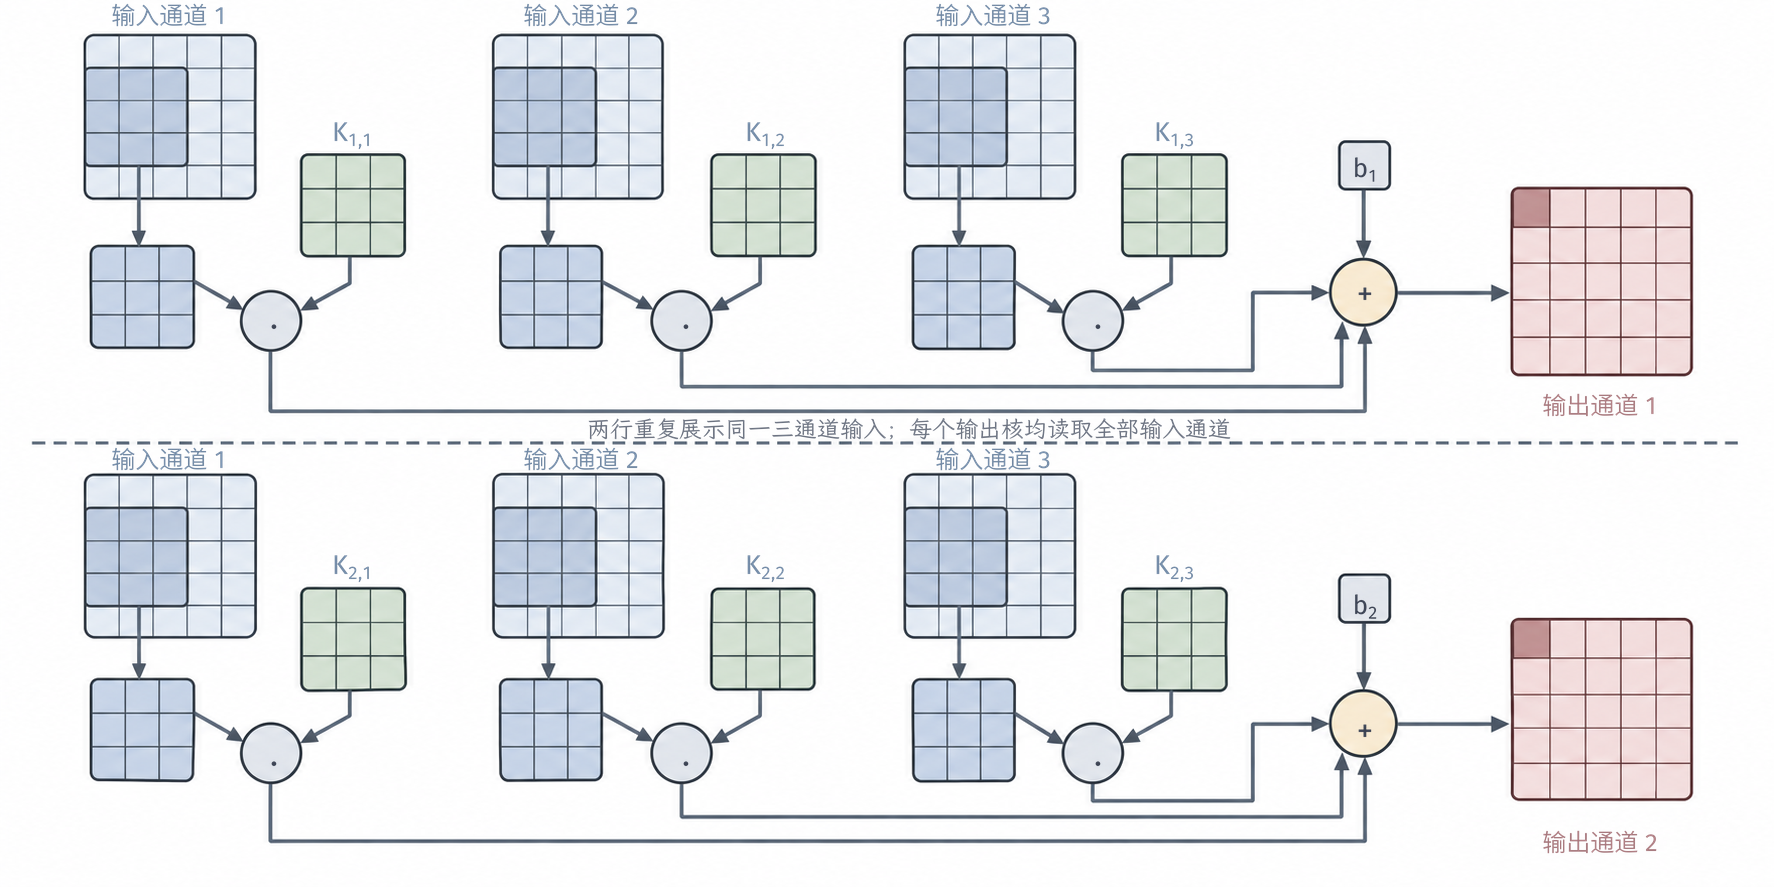
\includegraphics[width=150.199mm]{figures/05-neural-network-models/00-shared/generated/cnn-channels/figure.png}
  \caption{三输入、两输出通道的卷积。每行展示同一输入张量$\bm X$的三个通道；一组输出核包含三个通道切片，各自读取对应输入通道中高亮的局部窗口。各切片完成局部乘加后，三项贡献与偏置一起求和，分别写入右侧输出张量$\bm Z$的两个通道；两个输出平面分别由核1、核2产生。网格只示意通道与局部窗口的关系，不声明实际空间尺寸、步长或填充；核在空间位置间共享，输出尺寸由正文公式确定。}
  \label{fig:cnn-channels}
\end{figure*}

普通卷积层的参数数为
\begin{equation}
  p_{\mathrm{conv}}=k_hk_wc_{\mathrm{in}}c_{\mathrm{out}}
                    +c_{\mathrm{out}}\text{。}
  \label{eq:cnn-layer-parameters}
\end{equation}
空间尺寸没有出现在该式中，却仍出现在式\eqref{eq:cnn-direct-cost}的计算量和活动值存储量中。较大图像可以使用相同参数，但要生成更多响应。因此参数量由核形状决定，计算量和活动值内存还随空间网格扩大。

核为$1\times1$时，每个输出只读取同一空间位置的通道向量。\term{逐点卷积}（pointwise convolution）因此是所有位置共享的通道变换，可以增加、压缩或混合通道，却不直接扩展空间感受野。\term{分组卷积}（grouped convolution）把输入、输出通道分成$g$组，各组只在内部连接；若两类通道数都能被$g$整除，权重数变为$k_hk_wc_{\mathrm{in}}c_{\mathrm{out}}/g$。若每个输入通道单独使用一个空间核，再接逐点卷积混合通道，就得到一种\term{深度可分离卷积}（depthwise separable convolution）：将空间处理与通道混合分成两步。在每个输入通道产生一张中间图的设置下，权重数为$k_hk_wc_{\mathrm{in}}+c_{\mathrm{in}}c_{\mathrm{out}}$，但两步施加的结构约束也与普通卷积不同。

分组卷积的权重数可以按组逐一核算。每组有$c_{\mathrm{in}}/g$个输入通道和$c_{\mathrm{out}}/g$个输出通道，每个组内通道对需要$k_hk_w$个空间权重，因此一组有$k_hk_w(c_{\mathrm{in}}/g)(c_{\mathrm{out}}/g)$个权重。再乘以$g$组，便得到上面的除以$g$的结果。减少的连接也限制了这一层的信息流：某组的输出只能读取同组输入，其他组的信息需要在后续安排跨组混合的操作才能传入。

深度可分离配置则要分别计算两步。逐通道阶段有$c_{\mathrm{in}}$个空间核，每个核含$k_hk_w$个权重，共$k_hk_wc_{\mathrm{in}}$个；它产生$c_{\mathrm{in}}$张中间特征图。逐点阶段的每个输出通道都读取这$c_{\mathrm{in}}$个中间通道，因而需要$c_{\mathrm{in}}c_{\mathrm{out}}$个权重，两项相加就是前述总数。这里每个输入通道产生的中间特征图数为一，即图中所说的深度乘子为一；采用更大的乘子时，中间通道数及两部分权重数都要相应增加。这些权重计数均忽略偏置。

两步分工也说明了结构约束。逐通道阶段先为每个输入通道提取一种空间响应，逐点阶段只在同一位置组合这些响应。若两步之间不加非线性，对固定的输入通道，通往各输出通道的等效空间核只能是该逐通道核的不同倍数；普通卷积则允许每一对输入、输出通道独立设置空间核。因而，参数较少来自对可用空间变换的限制，不能仅凭输入、输出形状相同就把两种层视为等价。

图~\ref{fig:cnn-channel-connectivity-comparison}固定四个输入与四个输出通道，比较通道连接的改变。三个配置采用相同空间核，但读取的通道集合不同；深度可分离配置还通过后续逐点变换建立跨通道交互。

\begin{figure*}[htbp]
  \centering
  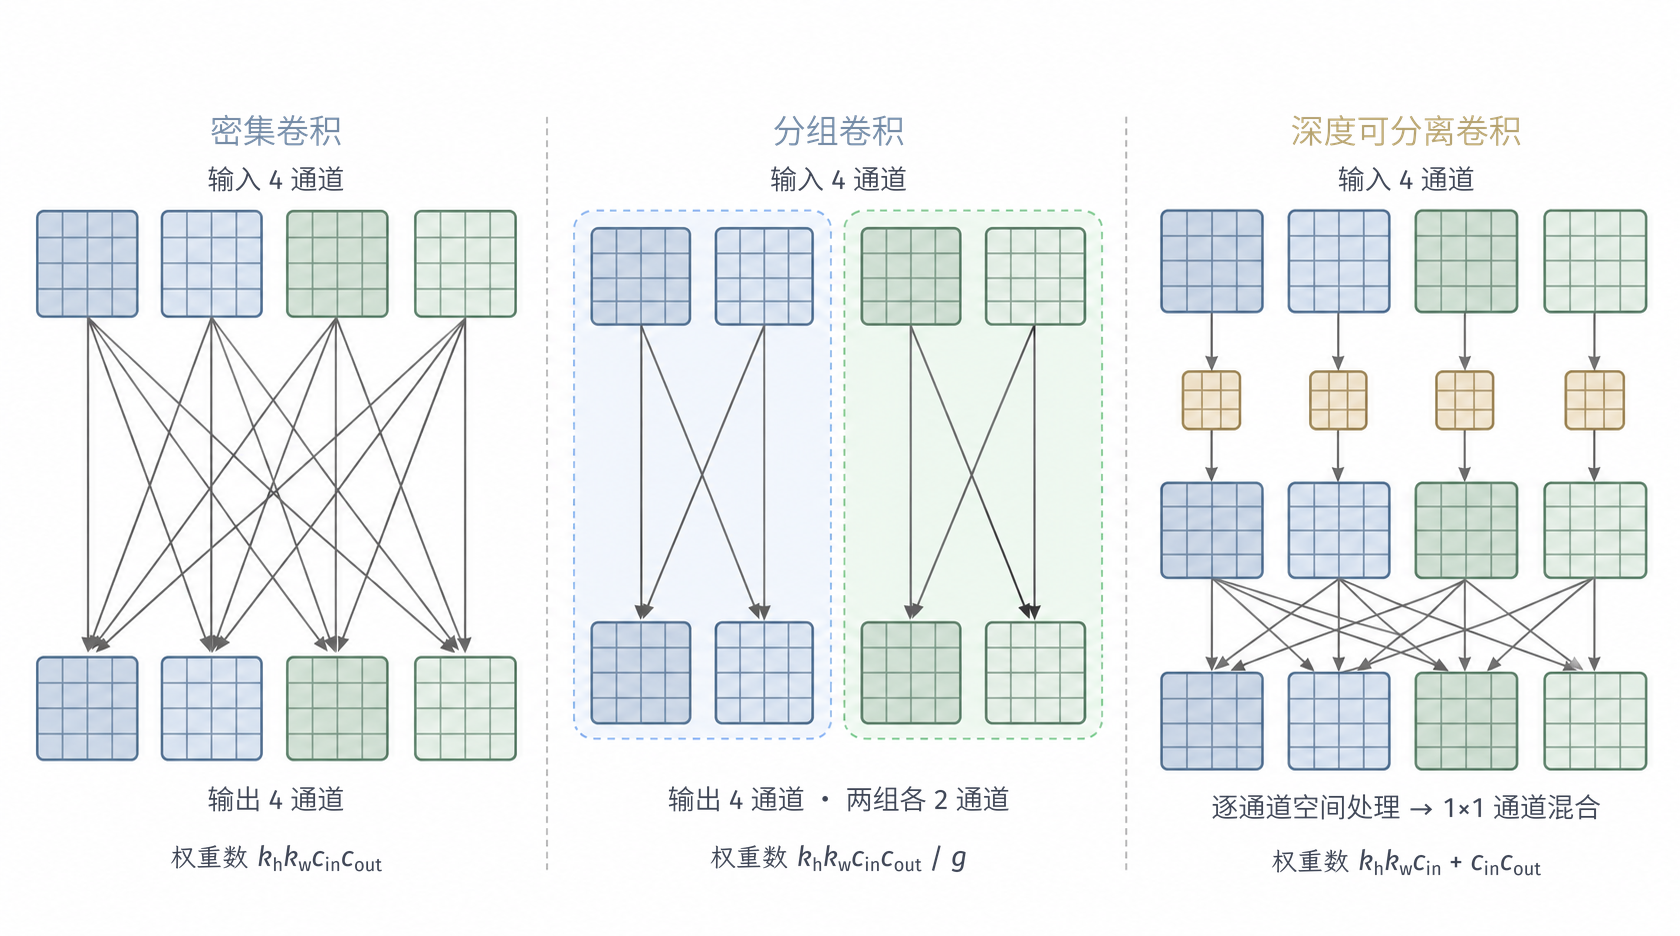
\includegraphics[width=142.240mm]{figures/05-neural-network-models/00-shared/generated/cnn-channel-connectivity-comparison/figure.png}
  \caption{四输入、四输出通道上的三种连接。密集卷积读取所有输入通道；两组卷积仅在各组内部连接；深度可分离卷积先逐通道完成空间处理，再用$1\times1$卷积混合通道。权重数忽略偏置，分组数为二，深度乘子为一。}
  \label{fig:cnn-channel-connectivity-comparison}
\end{figure*}
\FloatBarrier

多层组合让一个高层单元读取更大的输入范围。沿由局部卷积、局部池化和逐点运算组成的单条串联路径，设第$\ell$层的有效核尺寸为$e_\ell$、步长为$s_\ell$，$r_\ell$表示感受野跨度，$j_\ell$表示相邻响应在原输入上的间距。对一个轴，有
\begin{equation}
  r_0=j_0=1,\qquad
  r_\ell=r_{\ell-1}+(e_\ell-1)j_{\ell-1},\qquad
  j_\ell=s_\ell j_{\ell-1}\text{。}
  \label{eq:cnn-receptive-field}
\end{equation}
新增的$e_\ell-1$个间隔，每个在原输入上跨越$j_{\ell-1}$个位置，所以要相乘。以两个空洞率一、步长一的$3\times3$层为例，沿任一轴代入$e_1=e_2=3$和$s_1=s_2=1$，得到
\[
  \begin{aligned}
    r_1&=1+(3-1)\times1=3,& j_1&=1\times1=1,\\
    r_2&=3+(3-1)\times1=5,& j_2&=1\times1=1\text{。}
  \end{aligned}
\]
第二层读取三个相邻的第一层响应，它们各覆盖三个原输入位置，覆盖范围每次只平移一个位置，因此合起来是五个位置，而非九个。高、宽两轴分别计算，便得到$5\times5$；再接同样的一层则为$7\times7$。

若只把第一层的步长改为二，仍有$r_1=3$，但$j_1=2\times1=2$，第二层于是得到$r_2=3+(3-1)\times2=7$、$j_2=1\times2=2$。这里第二层窗口内的相邻响应在原输入上相隔两个位置，故覆盖$7\times7$。一般地，$j_{\ell-1}=\prod_{a=1}^{\ell-1}s_a$是此前各层步长的乘积，空乘积取一；它把当前层的间隔换算回原输入尺度。

这是忽略跨空间统计等非局部操作后的几何感受野；实际梯度和学到的权重可能集中在其中一部分，空洞采样也可能使范围内存在未读取的位置。含归一化的网络还需计入统计量带来的额外依赖，见第~\ref{sec:cnn-activation-normalization}节。填充决定响应中心对应哪个输入位置，边界响应的实际读取范围还会被原图尺寸截断。

\FloatBarrier

\subsection{池化层}
\label{sec:cnn-pooling}

卷积层在每个位置都保留一份局部响应，但后续判断有时并不需要知道某个特征\emph{具体在窗口里的哪个位置出现}，只关心它\emph{是否出现、有多强}。例如判断一张图里有没有眼睛，眼睛在感受野内偏左几个像素往往无关紧要。\term{池化}（pooling）就是对一个小窗口内的数值按某种固定规则汇聚成一个摘要值，通常对每个通道独立进行。它与卷积一样滑动窗口，但有两点本质区别：标准池化\emph{不含可学习权重}（汇聚规则是预先固定的），也\emph{不跨通道混合}。池化一方面逐步缩小空间尺寸、扩大后续单元的相对感受野并降低计算量，另一方面为网络提供了对特征小幅位移的容忍度——这正是从“位置敏感的卷积特征”走向“位置不敏感的类别判断”的关键一环。

设输出位置$(i,j)$在某通道读取的非空有效输入位置集合为$\Omega_{i,j}$，其元素个数为$q_{i,j}$。\term{最大池化}（max pooling）保留窗口内的最大响应，\term{平均池化}（average pooling）保留窗口内的平均响应：
\begin{equation}
  \begin{aligned}
    y_{i,j,c}^{\mathrm{max}}&=\max_{(u,v)\in\Omega_{i,j}}x_{u,v,c},\\
    y_{i,j,c}^{\mathrm{avg}}&=\frac1{q_{i,j}}
                   \sum_{(u,v)\in\Omega_{i,j}}x_{u,v,c}\text{。}
  \end{aligned}
  \label{eq:cnn-local-pooling}
\end{equation}
在式\eqref{eq:cnn-matrix-example}上用不重叠的$2\times2$窗口、步长二且不填充，分别得到
\begin{equation}
  \bm Y^{\mathrm{max}}=\begin{bmatrix}6&8\\14&16\end{bmatrix},\qquad
  \bm Y^{\mathrm{avg}}=\begin{bmatrix}3.5&5.5\\11.5&13.5\end{bmatrix}\text{。}
  \label{eq:cnn-pooling-example}
\end{equation}
最大池化侧重最强响应，平均池化反映整体水平。两者都丢失窗口内的部分信息：仅凭$6$不能知道该窗口的其他三个值，仅凭$3.5$也不能知道四个值的排列。

采用相同窗口与完整窗口取整规则时，池化的输出尺寸可由式\eqref{eq:cnn-output-size}计算。边界规则却要单独核对：最大池化常将无效位置排除，等价于用负无穷填充，而补零会改变全负窗口的最大值；平均池化若把补零位置计入分母，边缘均值会与只除以有效元素数不同。使用向上取整的接口还会保留末尾窗口，并对其边界另作处理；这会给出与本章向下取整约定不同的形状。

\term{全局平均池化}（global average pooling）把每张特征图汇成一个数，得到通道向量$\bm r\in\mathbb R^{c_{\mathrm{in}}}$：
\begin{equation}
  r_c=\frac1{hw}\sum_{i=0}^{h-1}\sum_{j=0}^{w-1}x_{i,j,c}\text{。}
  \label{eq:cnn-global-average-pooling}
\end{equation}
全局最大池化则保留每个通道在全部位置上的最大值。若平移仅对特征图作位置置换，例如循环边界上的整数平移，这两种汇聚都保持结果不变。实际网络中的填充、裁剪和跨步可能改变平移后的特征值和采样位置，此时上述置换条件不再成立。局部池化保留的是窗口中的最大值或平均值，其平移性质也由窗口如何移动决定。

\subsection{激活与归一化}
\label{sec:cnn-activation-normalization}

卷积层本身仍是“加权求和加偏置”的仿射映射，单独堆叠再多也退化为一次仿射，因此卷积之后同样要接非线性激活。ReLU、GELU或SiLU可逐元素作用于特征图，既保留空间和通道形状，又引入非线性。它们的定义、梯度以及与初始化的配合见第~\ref{sec:ffn-activations}节；这里不重复，只强调分工：隐藏层激活决定局部特征如何组合，而末端输出取什么范围（概率还是连续值）由具体任务另行规定。

深层网络在训练中还有一个与激活密切相关的困难：随着前面各层参数不断更新，每一层收到的输入分布都在持续变化，后层不得不反复“追赶”移动的输入尺度；若某些通道的数值变得过大或过小，还容易把Sigmoid、Tanh推入饱和区，拖慢学习。一种直接的想法是，在每一层内部主动把活动值重新拉回到稳定的中心和幅度，再让网络学习如何缩放、平移回去。\term{批归一化}（batch normalization, BN）正是这种做法：它用当前小批量的统计量把特征标准化，再额外学习一个缩放系数和平移量，使网络仍有表达自由度。对卷积特征，均值和方差通常\emph{按通道}、在批量轴和两个空间轴上一起统计；设小批量预激活为$z_{t,i,j,c}$、样本索引$t=1,\ldots,n_{\mathrm b}$，参与统计的元素总数为$m=n_{\mathrm b}h'w'$，则
\begin{equation}
  \begin{aligned}
    \mu_c&=\frac1m\sum_{t,i,j}z_{t,i,j,c},\qquad
    v_c=\frac1m\sum_{t,i,j}(z_{t,i,j,c}-\mu_c)^2,\\
    \widehat z_{t,i,j,c}&=\frac{z_{t,i,j,c}-\mu_c}{\sqrt{v_c+\epsilon}},\qquad
    \bar z_{t,i,j,c}=\gamma_c\widehat z_{t,i,j,c}+\beta_c\text{。}
  \end{aligned}
  \label{eq:cnn-batch-normalization}
\end{equation}
其中$\epsilon>0$防止分母过小。固定通道$c$后，均值与方差汇集全部$n_{\mathrm b}h'w'$个数值，不跨通道求和；同一组可学习参数$\gamma_c,\beta_c$也在这些样本和空间位置之间共享，不为每个像素位置另设一组参数。

全连接前馈网络的BN使用相同原则，但没有空间轴。将一个小批量的特征按行排成$\bm Z_{\mathrm{FFN}}\in\mathbb R^{n_{\mathrm b}\times d}$，固定特征坐标$q$，就只在$\{z_{t,q}:t=1,\ldots,n_{\mathrm b}\}$上统计均值与方差，$\gamma_q,\beta_q$在样本间共享。因此，FFN的“特征级”BN固定一列、跨样本统计，CNN的“通道级”BN固定一个通道、跨样本和空间位置统计。若把卷积特征展平成$n_{\mathrm b}\times(h'w'c_{\mathrm{out}})$后逐列做BN，每个空间位置会分别统计并拥有各自的仿射参数，这与卷积BN不同。其他归一化方法的统计轴对照见图~\ref{fig:training-normalization-axes}。

训练时，共用均值与方差使这些数值的计算相互耦合：一个值改变，可能影响同组其他值的归一化结果。CNN的这种依赖既跨样本，也跨同一通道的空间位置。推理时通常使用训练中累计的均值与方差，使单样本计算固定。累计统计量按实现选定的估计规则更新。常见组合是“卷积—BN—ReLU”，后接BN的卷积层偏置常可省略，因为通道中心化会消除它，BN另有平移参数\scite{ioffe2015batchnorm}

批内独立图像变少时，BN的均值与方差可能更依赖当前批的组成，同一张图像的归一化结果也会随同批其他图像改变。若希望归一化不再读取其他样本，就需要改用单个样本内部的统计量。

当批量较小或批内组成变化较大时，可以改变统计范围。\term{组归一化}（group normalization, GN）把通道分成若干组，对每个样本分别在一组通道及其空间位置上统计均值和方差，然后仍按通道学习缩放与平移。它不需要其他样本提供统计量，训练和推理使用相同的统计范围，但会让同组通道发生统计耦合。组数是结构设置，通道数需要能够均分。GN与BN的区别首先在统计对象：前者独立处理样本，后者使用批内信息。实际训练效果还随任务和批量设置变化\scite{wu2018groupnorm}

这些统计量也改变数据依赖范围。训练态BN通过通道均值与方差连接同批样本的不同空间位置，GN则在训练和推理时都连接同一样本组内的各空间位置；式\eqref{eq:cnn-receptive-field}没有计入这些路径。推理态BN若使用固定的运行统计量，就只是逐点仿射变换，不会额外扩大依赖范围。

归一化、激活和池化的顺序影响计算含义。对平均池化，通常有$\sigma(\operatorname{Avg}(\bm X))\neq\operatorname{Avg}(\sigma(\bm X))$；例如两个响应为$-2$和$1$时，先平均再ReLU得到$0$，先ReLU再平均得到$1/2$。单调逐点激活与不含额外填充值的最大池化可以交换；归一化还读取组内统计量，改变顺序就可能改变输出。各架构因而用明确的模块顺序确定计算；跨架构的训练机制由后续《神经网络的训练》章展开。

\subsection{输出和学习目标}
\label{sec:cnn-output-objectives}

经过若干“卷积—激活—池化”的堆叠，网络得到的还是一张张带空间位置的特征图，而不是最终答案。如何把这些空间特征变成预测，取决于任务要不要保留位置：\emph{整图分类}要把所有空间信息汇聚成一个类别，\emph{逐像素任务}则必须在每个位置给出答案。这一小节给出两种末端的接法；它们复用的是同一套卷积特征，区别只在最后是否丢弃空间轴。

预测整张图像的类别时，需要把空间特征转换为整体得分。可以将末层特征展平后接全连接层，也可以先作全局平均池化再接分类层。设汇聚向量为$\bm r$，类别数为$q$，原始得分为$\bm a=\bm U\bm r+\bm d\in\mathbb R^q$，则多类概率与单样本损失为
\begin{equation}
  p_k=\frac{\exp(a_k)}{\sum_{v=1}^{q}\exp(a_v)},\qquad
  \ell=-\log p_y\text{。}
  \label{eq:cnn-image-classification}
\end{equation}
这里$y\in\{1,\ldots,q\}$为图像标签；训练学习卷积特征与分类层参数，使用时取最大得分类别。回归、二分类和多标签输出可以沿用第~\ref{sec:ffn-output-objectives}节的变换与损失。分类输出的概率由这组类别得分共同归一化，最后一张特征图的数值本身仍是内部响应。

若要预测每个像素的类别，就需要保留或恢复空间轴。设得分张量为$\bm A\in\mathbb R^{h\times w\times q}$，在每个位置单独应用Softmax，可得到$p_{i,j,k}$。给定像素标签$y_{i,j}$，逐位置交叉熵为
\begin{equation}
  \ell_{\mathrm{seg}}=-\frac1{|\Omega|}
    \sum_{(i,j)\in\Omega}\log p_{i,j,y_{i,j}}\text{。}
  \label{eq:cnn-segmentation-loss}
\end{equation}
其中$\Omega$为非空的有标签位置集合，未标注像素不参与求和。每个位置输出多个颜色值或其他连续量时，可改用回归损失。两种输出任务都用卷积特征，却对空间汇聚有不同要求：分类可以舍去具体位置，分割和图像生成必须保留输出与位置之间的对应。

对$n$个独立训练样本，用$\bm\theta$收集所有可学习核、偏置、归一化参数和输出层参数。若网络不含跨样本操作，前向映射可逐样本计算，经验目标可写为
\begin{equation}
  \widehat R_S(\bm\theta)=\frac1n\sum_{t=1}^{n}
    \ell\!\left(\bm f_{\bm\theta}(\bm X_t),\bm Y_t\right)\text{。}
  \label{eq:cnn-training-objective}
\end{equation}
这里$\bm Y_t$统指与任务对应的目标；标量类别标签按式\eqref{eq:cnn-image-classification}处理。像素损失可在单张图像内部先汇聚，再在图像之间取平均。

使用固定统计量的推理态BN符合上述逐样本前向条件，训练态BN则不符合。给定非空批索引集$B$，将整批输入记为$\bm X_B=(\bm X_t)_{t\in B}$，用$\bm F_{\bm\theta}(\bm X_B)_t$表示批预测中对应样本$t$的输出。一次更新所用的数据损失为
\begin{equation}
  L_B(\bm\theta)=\frac1{|B|}\sum_{t\in B}
    \ell\!\left(\bm F_{\bm\theta}(\bm X_B)_t,\bm Y_t\right)\text{。}
  \label{eq:cnn-batch-objective}
\end{equation}
各项损失仍可相加，但每项预测都可能依赖整批输入。求导沿完整批计算图回传，包括均值与方差连接不同样本的路径。分别运行单样本前向会改变归一化统计量及其导数，求导后再平均得到的量一般不同于$\nabla_{\bm\theta}L_B$。若要定义随机分批训练的总体目标，还需给定批抽样规则，再对$L_B$取期望；梯度累积与一次大批前向的区别见第~\ref{sec:training-inexact-gradients}节。正则项、数据增强和优化策略可以加入训练过程，本章重点是结构特有的梯度与信息传递。

\FloatBarrier

\subsection{常见卷积网络架构}
\label{sec:cnn-classic-architectures}

完整架构要在空间精度、特征种类和计算成本之间分配资源。下采样减少空间位置，高层增加通道可以在较粗网格上保存更多特征；末端再根据任务读出。LeNet、AlexNet、VGG和GoogLeNet分别体现了局部到整体、容量扩大、规则小核和多尺度分支的组织方式。图中叠片表示特征张量，正面示意空间网格，叠片示意通道维；深色局部块与算子内部的虚线突出一次局部映射。下方细节用层名对应主链中的算子，独立展示局部计算。全连接层用包含圆形神经元的平面方框表示。蓝色用于卷积特征与全连接，黄色用于池化或降采样，绿色用于少量卷积核细节。主路径从左向右展开，实际尺寸写在各层或阶段下方；绘图尺寸不与张量元素数严格成比例。

\subsubsection{LeNet-5：从局部检测到整体读出}
\label{sec:cnn-lenet}

手写字符的局部笔画需要逐渐组合成整字。LeNet-5交替使用卷积与降采样，先形成小范围响应，再扩大后层能够读取的区域。原网络接收$32\times32$的单通道图像，C1用六个$5\times5$核产生$28\times28\times6$特征；S2降为$14\times14\times6$，C3产生$10\times10\times16$，S4再降为$5\times5\times16$。C5用覆盖整个$5\times5$区域的核得到120个整体特征，接84单元的F6，再计算十类输出，见图~\ref{fig:cnn-lenet}。

F6的84个输出组成表示向量$\bm h\in\mathbb R^{84}$\scite{lecun1998}。原网络为十个类别分别设置同维的参考向量$\bm v_k$，将同一个$\bm h$逐一与它们比较。欧氏径向基函数（Euclidean radial basis function, RBF）读出计算的是平方欧氏距离：
\[
  d_k=\sum_{j=1}^{84}(h_j-v_{k,j})^2
      =\lVert\bm h-\bm v_k\rVert_2^2,
  \qquad k=1,\ldots,10\text{。}
\]
$d_k$越小，表示与第$k$类参考向量越接近；只在这十类中作分类决策时，选择距离最小的类别。原论文按字符的$7\times12$位图设置参考向量，分量为$-1$或$+1$，并至少在初始阶段保持这些向量固定，84维正来自这84个位置。F6需要学习把输入映射到与目标类别参考向量相近的位置。这十个输出是类别不匹配的惩罚值，其大小方向与前节的分类得分相反，也没有直接给出和为一的类别概率。

\begin{figure*}[htb]
  \centering
  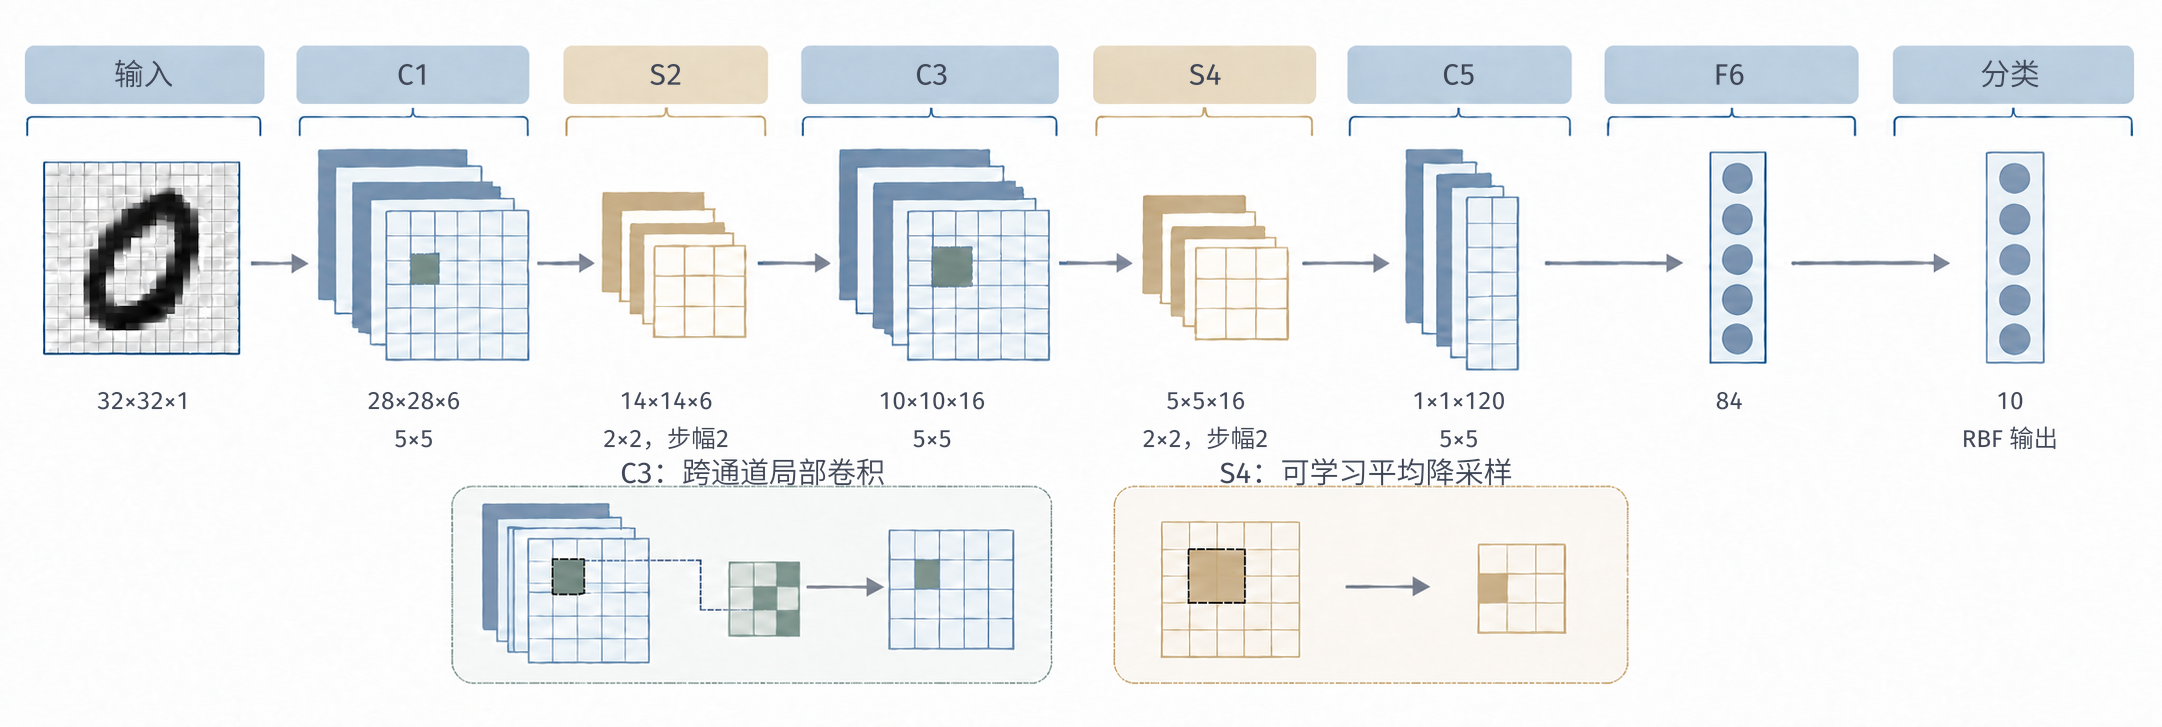
\includegraphics[width=169.000mm]{figures/05-neural-network-models/00-shared/generated/cnn-lenet/figure.png}
  \caption{LeNet-5的层次结构。特征张量用叠片表示，层名与空间、通道尺寸标注在对应图元附近。C1、C3、C5为卷积层，S2、S4为可学习的平均降采样层，F6含84个单元，原始十类读出采用欧氏径向基函数。下方分别展开C3的跨通道局部卷积和S4的平均降采样；网格、叠片数和节点数均为示意，尺寸标签给出真实形状，C3部分通道连接未逐条展开。}
  \label{fig:cnn-lenet}
\end{figure*}

S2和S4采用可学习的降采样：每张特征图的局部求和还经过可学习缩放、偏置和非线性。C3采用指定的部分通道连接，不同输出读取不同的输入组合。C5虽然空间输出为$1\times1$，仍是卷积层；对这里固定的输入形状，它恰好具有整体连接的作用\scite{lecun1998}

教学中常见的“普通卷积—平均池化—ReLU—Softmax”版本使用现代算子重写了这条处理链。它仍按局部检测、空间缩小和整体读出组织计算，但降采样参数、通道连接和输出规则已改变。具体版本由这些计算约定共同确定。

\subsubsection{AlexNet：扩大容量并组织GPU训练}
\label{sec:cnn-alexnet}

自然图像包含更多颜色、纹理和尺度变化，需要更丰富的局部表示。AlexNet包含五个卷积层和三个全连接层；隐藏层使用ReLU，在第一、第二和第五个卷积阶段后作最大池化，在前两个全连接层使用Dropout。卷积主体输出通道依次为$96,256,384,384,256$，前两层分别用较大核快速扩大覆盖范围，后三层用$3\times3$继续组合特征\scite{krizhevsky2012}

图~\ref{fig:cnn-alexnet}采用能明确核算形状的$227\times227$教学输入约定。所有卷积不使用空洞，卷积与池化的空间尺寸均按式\eqref{eq:cnn-output-size}向下取整；三次最大池化均为$3\times3$窗口、步长二、无填充。首层卷积以$11\times11$核、步长四、无填充产生$55\times55$输出，池化降到$27\times27$；第二卷积使用$5\times5$核、步长一、四周各填充二，保持尺度，池化降到$13\times13$；后三层均为$3\times3$核、步长一、四周各填充一，保持该尺度。末次池化形成$6\times6\times256$，展平为9216维，接4096、4096和1000单元。原论文正文写输入$224\times224$，却展示首层55的空间尺寸；在无填充的向下取整规则下二者并不相符。图和本节形状计算统一采用227输入。

\begin{figure*}[htb]
  \centering
  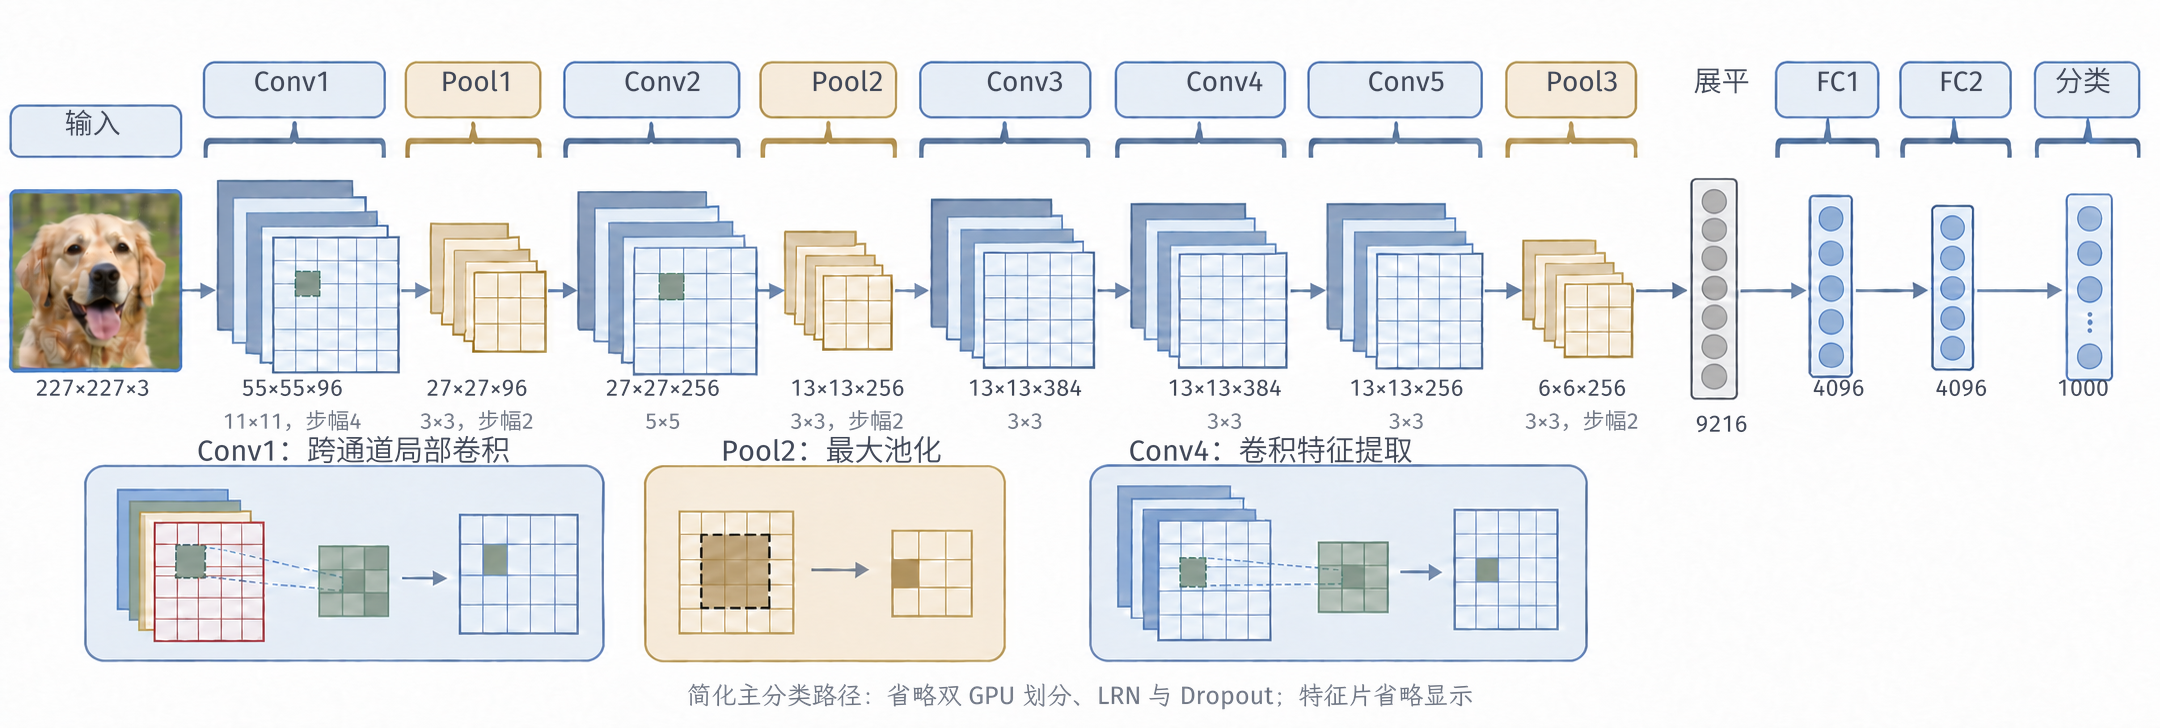
\includegraphics[width=169.000mm]{figures/05-neural-network-models/00-shared/generated/cnn-alexnet/figure.png}
  \caption{AlexNet的五个卷积层与三个全连接层。全部主路径在一行展开，卷积层、最大池化层与全连接层分别绘出；最后一次池化的输出展平为9216维。各层下方给出空间尺寸和通道数，Conv表示卷积，Pool表示池化。下方依次展开Conv1的跨通道卷积、Pool2的最大池化和Conv4的卷积特征提取。网格、叠片和卷积核仅作局部映射示意，各层的实际尺寸与步幅以主链标注为准。此图采用227输入及正文给定的填充约定，省略局部响应归一化、Dropout和原始双GPU的分组细节。}
  \label{fig:cnn-alexnet}
\end{figure*}

容量增加也会把成本集中到尾部。仅9216维到4096维的全连接权重就有$37748736$个，下一层又有$16777216$个；它们与卷积核共享权重的组织不同，是全模型参数量的重要来源。原实现将网络分配到两块GPU，部分层限制跨GPU的通道连接，这也影响了分组方式。ReLU、数据增强和Dropout分别作用于非线性、训练输入变化与正则化；GPU让这些运算可以实际执行，训练设计则规定了参数如何由数据学得。这些条件共同支撑了这套大规模监督系统。

\subsubsection{VGG：以连续小核组织深度}
\label{sec:cnn-vgg}

AlexNet混合不同核尺寸，VGG则研究较规则的小核堆叠。主体使用步长一、填充一的$3\times3$卷积，在阶段末用$2\times2$、步长二的最大池化缩小空间。VGG-16的五个阶段分别含$2,2,3,3,3$个卷积层，通道数为$64,128,256,512,512$；加上三个全连接层，共有16个带权重的层，池化与激活不计入这个数字。VGG-19把后三阶段的卷积数增为四，总计19个带权重层\scite{simonyan2015vgg}

\begin{figure*}[htb]
  \centering
  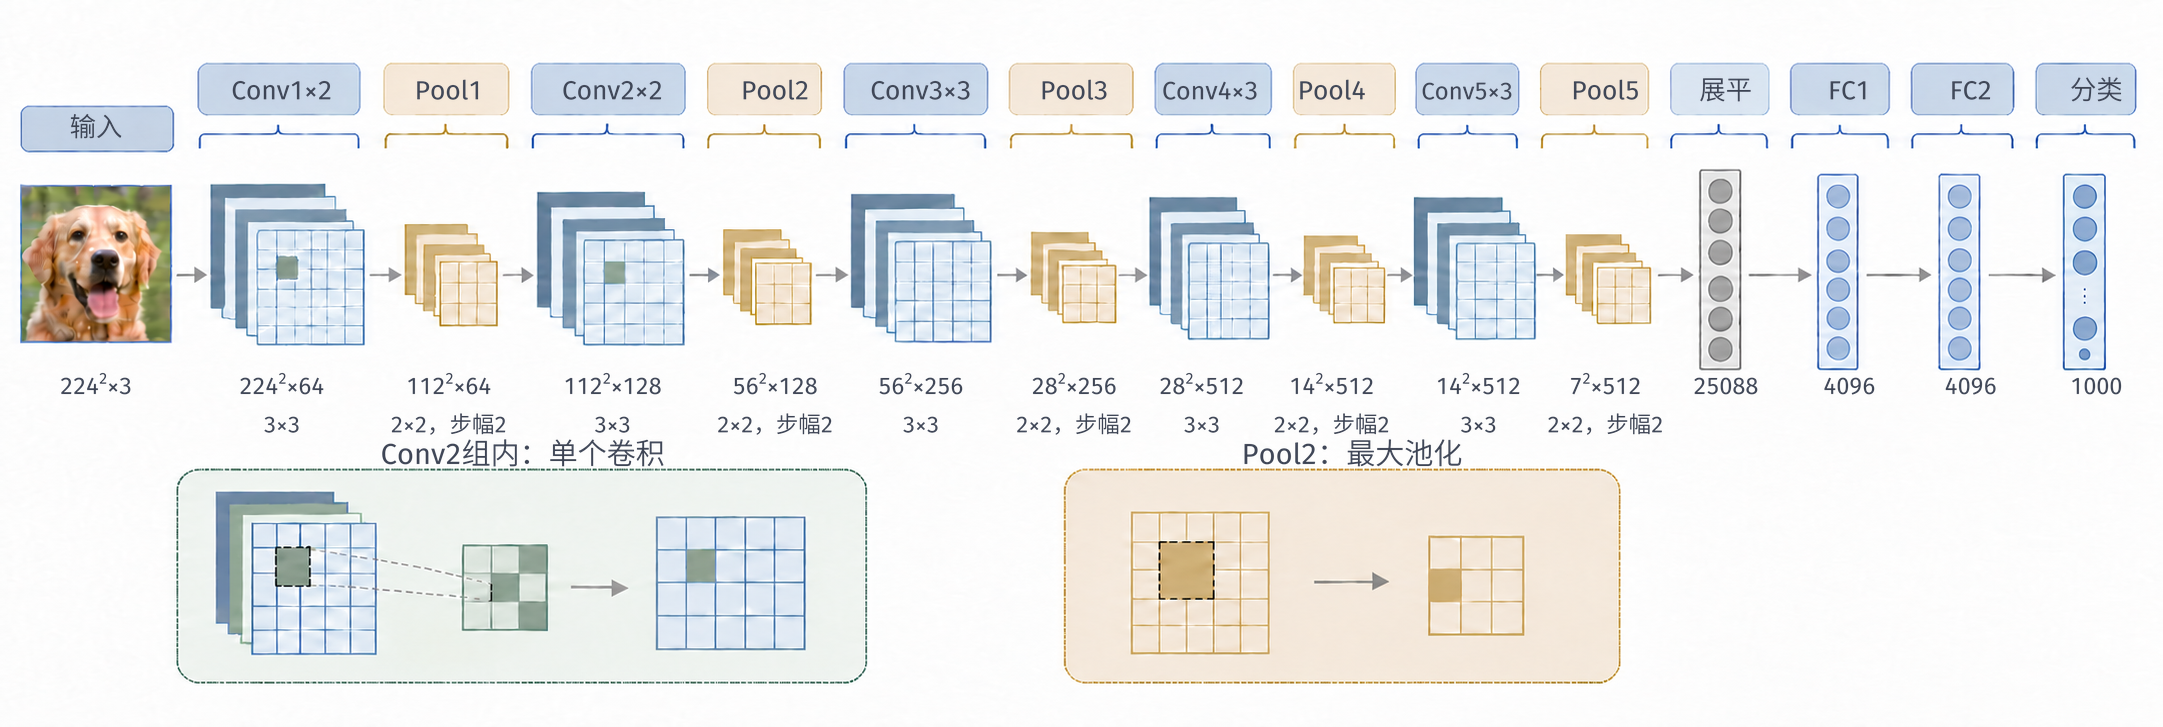
\includegraphics[width=169.000mm]{figures/05-neural-network-models/00-shared/generated/cnn-vgg/figure.png}
  \caption{VGG-16的五阶段卷积主体与全连接尾部。沿用AlexNet的特征叠片、池化、灰色展平及全连接图元；层名和尺寸分别置于对应图元上、下。每个Conv组包含标明次数的$3\times3$卷积并保持空间尺寸，其后的池化单独画出、使空间减半。下方展示Conv2组内单个卷积的代表性局部映射及Pool2的最大池化，并不将单个卷积等同于整个卷积组。13个卷积层加三个全连接层构成16个带权重层。网格、叠片数和节点数仅作示意；$a^2\times c$表示$a\times a\times c$。}
  \label{fig:cnn-vgg}
\end{figure*}

连续小核能够逐层扩大感受野。两个步长一的$3\times3$层覆盖$5\times5$跨度，三个覆盖$7\times7$；若各层通道均为$c$且忽略偏置，两个小核用$18c^2$个权重，单个$5\times5$用$25c^2$个。这个权重比较固定了各层通道数。两个小核之间还加入非线性，候选映射由此改变；相同感受野只描述读取范围。

\begin{figure}[htb]
  \centering
  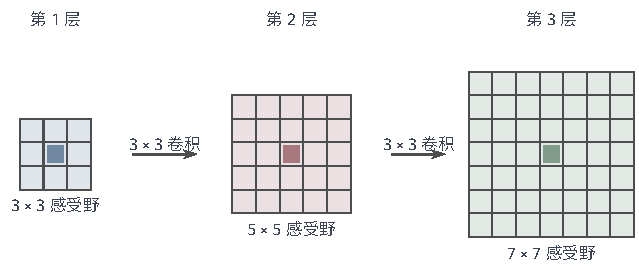
\includegraphics[width=108.158mm]{figures/05-neural-network-models/00-shared/tikz/cnn-receptive-field-stack/figure.pdf}
  \caption{三个步长一、无空洞的$3\times3$卷积逐层扩大几何感受野。彩色方格表示一个高层位置在原输入上可能读取的范围，中心实色格只用于对齐位置；跨度依次为$3,5,7$。图没有计入池化、跨位置归一化或边界填充造成的额外依赖。}
  \label{fig:cnn-receptive-field-stack}
\end{figure}

图~\ref{fig:cnn-receptive-field-stack}还可以沿反向的读取关系理解：第三层的一个位置读取第二层的九个位置，每个第二层位置又读取第一层的九个位置。相邻窗口彼此重叠，最外侧能够涉及原输入的$7\times7$区域。沿途的中间通道和激活决定怎样组合这个区域中的信息。因此，三个小核虽然与一个$7\times7$核具有相同的几何覆盖范围，却通过多次特征变换形成输出；仅凭覆盖范围，不能把两种映射视为等价。

从完整网络看，小核堆叠与阶段间池化承担不同作用。以$224\times224$输入为例，第一阶段的两个卷积始终在$224\times224$网格上组合特征，池化才把网格降到$112\times112$。第二阶段在这个较粗网格上学习128种特征，其后的池化再降到$56\times56$。图~\ref{fig:cnn-vgg}中的每个卷积组都按这个方式展开：组内改变特征内容，组间改变空间精度和后续计算规模。

空间缩小并不意味着卷积运算量按同样比例减少。对步长一的$3\times3$卷积，忽略边界差异，乘加次数约为$9hwc_{\mathrm{in}}c_{\mathrm{out}}$。若高、宽分别减半，同时输入、输出通道都加倍，空间位置数减少到四分之一，通道组合数却增至四倍，乘加次数大致不变；输出活动值数$hwc_{\mathrm{out}}$则减半。VGG各阶段的首层与通道不再增加的后层还要按实际形状单独核算，不能只用网格大小判断成本。

这种规则结构便于分阶段核算形状，但高分辨率阶段仍需保存大量活动值，经典VGG的4096单元全连接尾部也有大量参数。统一的小核安排了深度和读取范围，串联变换中的梯度传播与训练退化仍需通过学习方法和连接设计处理。

\subsubsection{GoogLeNet：在模块内分配多个尺度}
\label{sec:cnn-googlenet}

连续小核把不同尺度安排在不同深度。若希望同一层同时处理不同范围，可以把输入送入并行分支。\term{Inception模块}将同一输入分别交给$1\times1$、$3\times3$、$5\times5$局部处理及池化分支，再沿通道轴拼接。较大核前先用$1\times1$压缩通道，池化分支保持空间尺寸后也可用逐点卷积调节通道。各分支需要相同高、宽，通道数则可以不同，见图~\ref{fig:cnn-inception}。

\begin{figure*}[htb]
  \centering
  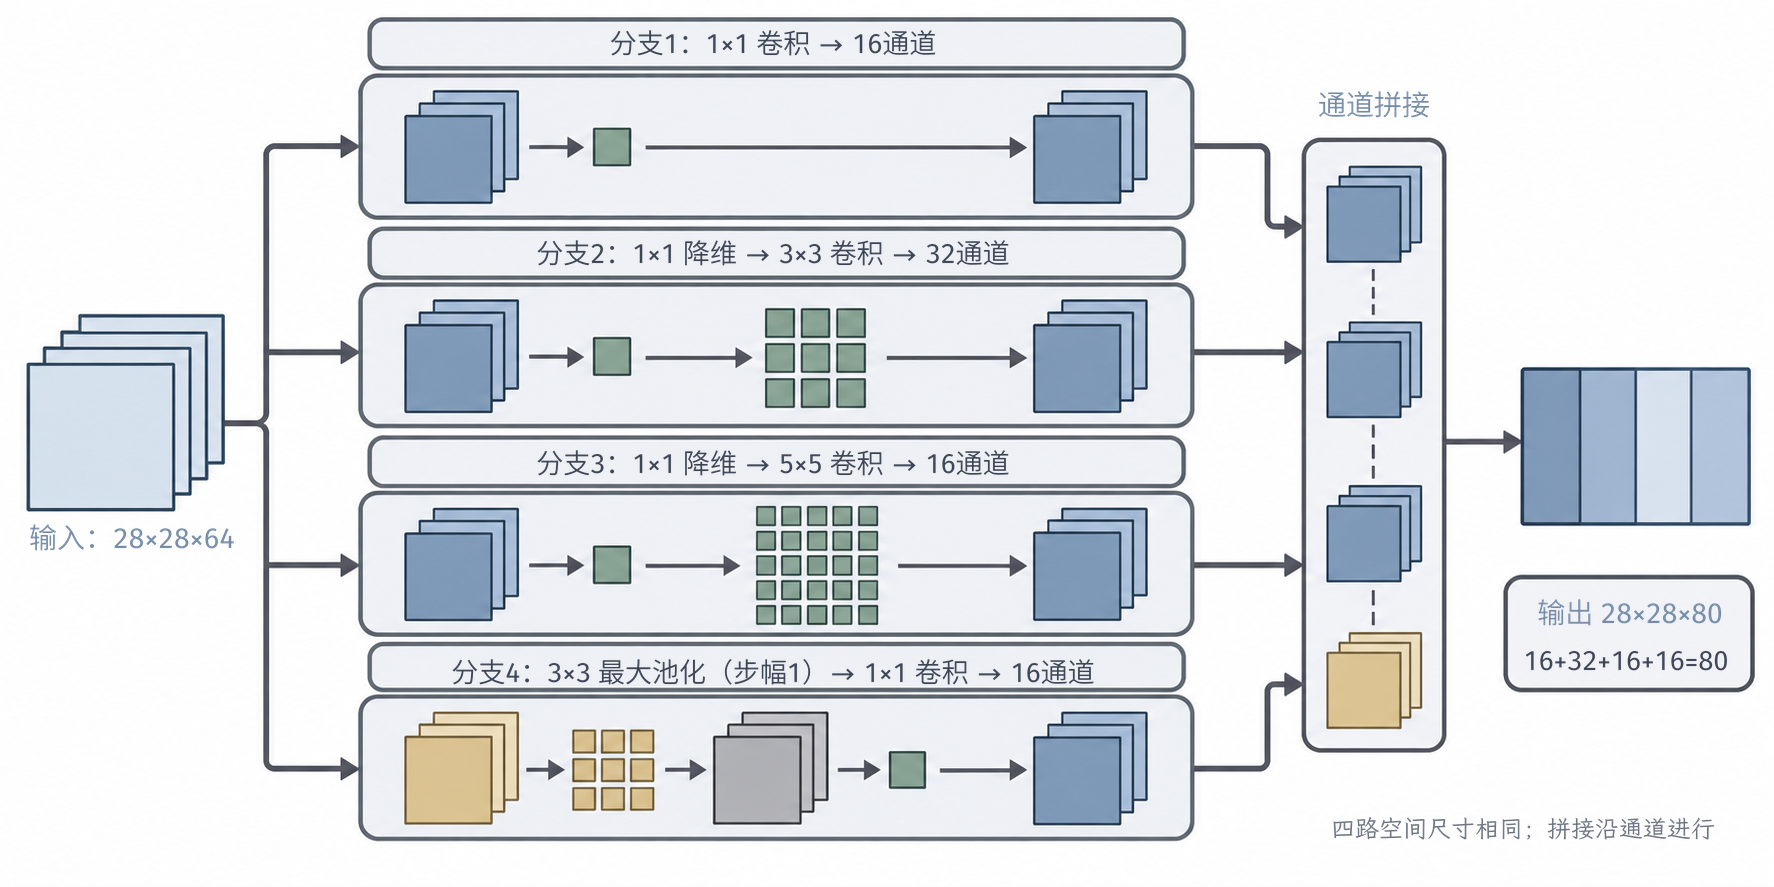
\includegraphics[width=150.199mm]{figures/05-neural-network-models/00-shared/generated/cnn-inception/figure.png}
  \caption{一个Inception模块的四分支教学配置。输入为$28\times28\times64$；四条分支分别输出16、32、16、16个通道，保持同一空间尺度，拼接得到$28\times28\times80$。中间的逐点卷积先压缩通道，最大池化采用步长一及same填充。圆角方框表示处理算子，各分支的标签给出核尺寸或通道数；右侧拼接框沿通道合并四路输出。四条路径实际并行，激活省略。}
  \label{fig:cnn-inception}
\end{figure*}

图中$3\times3$分支先将通道从64压到16，再输出32个通道，权重数为$64\times16+9\times16\times32=5632$；直接从64映射到32需要$18432$个。节省来自中间通道压缩，压缩也会限制该分支的表示。拼接保留分支间的区别，没有像相加那样把对应通道混合；后续卷积再学习如何组合这些通道。

可以固定一个空间位置，追踪四条分支怎样组成它的输出。逐点分支给出16个只在该位置混合通道的响应，另外两条卷积分支给出32个和16个结合周围位置的响应，池化分支再给出16个局部汇聚后的响应。拼接把这四组数依次放入一个80维向量。所有分支处理的是同一张空间网格，并未把图像分成四块；它们分配的是不同处理方式的通道数。下一模块的逐点卷积可以同时读取这80个数，学习哪些尺度的响应需要共同使用。

经典GoogLeNet先用普通卷积与池化形成$28\times28\times192$特征，再堆叠九个Inception模块，按两、五、两个模块分成三个尺度阶段；两个阶段间池化将空间降为14和7。末端$7\times7\times1024$特征经全局平均池化形成1024维向量，再作1000类分类。训练时，在中间层加入辅助分类器，让较浅位置也收到任务损失；推理时使用主分类路径。图~\ref{fig:cnn-googlenet}展示主路径，原论文按最长路径计22个带参数层，一个Inception模块内部则包含多条路径和多个卷积。

\begin{figure*}[htb]
  \centering
  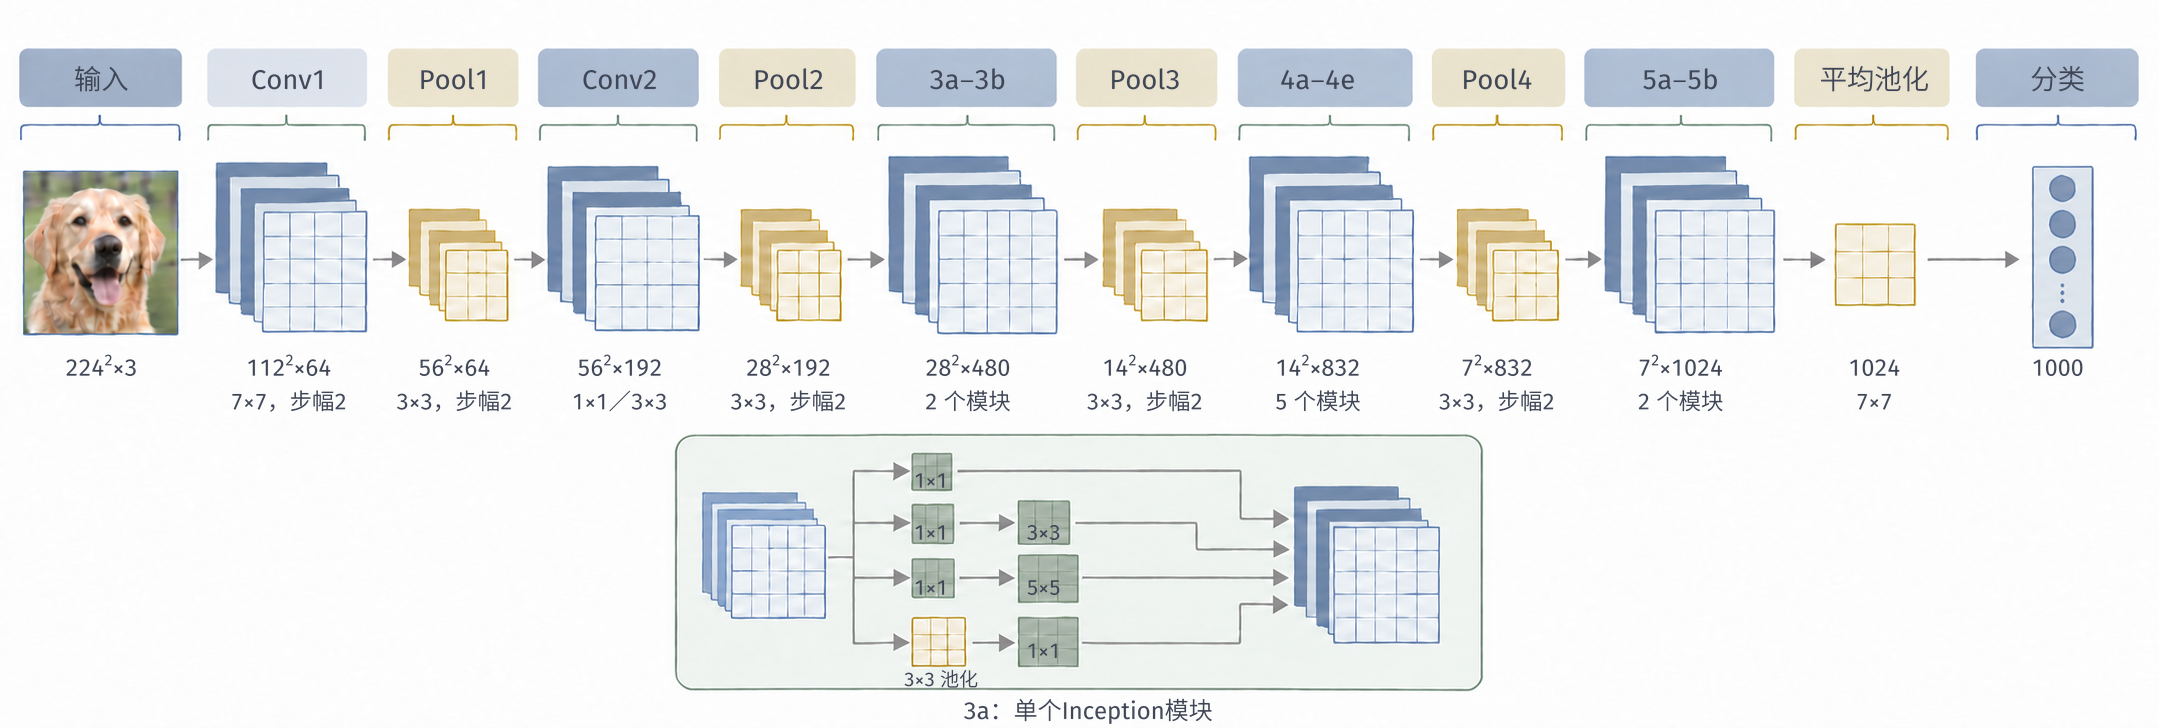
\includegraphics[width=169.000mm]{figures/05-neural-network-models/00-shared/generated/cnn-googlenet/figure.png}
  \caption{经典GoogLeNet的主分类路径。卷积前端把$224\times224$输入变成$28\times28\times192$；两个、五个、两个Inception模块组成三个阶段，阶段间池化改变空间尺度。各阶段末的通道数为480、832和1024，全局平均池化后接1000类分类器。辅助分类分支省略，下方以3a为代表展开单个Inception模块的四分支组织，主链的3a--3b组实际包含两个模块；分支机制见图~\ref{fig:cnn-inception}。}
  \label{fig:cnn-googlenet}
\end{figure*}

末端的全局平均池化还改变了分类层怎样使用位置。每个通道在$7\times7$网格上的49个响应先取平均，分类层只读取1024个通道均值。忽略偏置，这个1000类分类层有$1024\times1000$个权重；若把同一特征张量展平后直接接1000类输出，则需$49\times1024\times1000$个权重。减少来自先汇聚空间位置，但这种读出也舍去了同一通道内响应的具体位置：交换这些位置不会改变通道均值。网络须在汇聚前把分类所需的空间关系转化为通道响应；若任务本身需要逐位置答案，就应保留空间输出。

GoogLeNet用多分支增加同层处理方式，用逐点卷积控制大核分支的成本，并以全局汇聚替代庞大的全连接尾部。代价是分支调度、拼接和更多中间特征，理论乘加预算仍需结合实现分析\scite{szegedy2015googlenet}表~\ref{tab:cnn-classic-architectures}把四种架构放回共同的问题：它们如何从局部形成整体表示，又将计算与参数放在何处。

\begin{table*}[htb]
  \centering
  \begin{tabularx}{\linewidth}{@{}lXX@{}}
    \toprule
    架构 & 主体组织 & 理解结构时的侧重点\\
    \midrule
    LeNet & 卷积与可学习降采样交替 & 局部到整体；部分连接及原始输出约定\\
    AlexNet & 五个卷积层与较大全连接尾部 & 通道容量、训练机制、GPU分组及尾部成本\\
    VGG & 连续小核，阶段间池化 & 感受野、深度、规则结构及活动值成本\\
    GoogLeNet & 多尺度分支、通道压缩与拼接 & 同层并行处理、计算预算与整体汇聚\\
    \bottomrule
  \end{tabularx}
  \caption{经典卷积网络的组织方式。各行比较计算结构，没有在不同训练设置之间比较准确率。层数、输入形状和读出方式均应结合具体版本理解。}
  \label{tab:cnn-classic-architectures}
\end{table*}

\FloatBarrier

\section{参数学习}
\label{sec:cnn-learning}

卷积网络仍按前章的链式法则学习。结构带来的区别是：一个核权重在许多位置出现，一个输入又可能被多个窗口读取。因此，初始化应按局部连接数定尺度，反向传播则必须汇总所有重复使用的贡献。

\subsection{参数初始化}
\label{sec:cnn-initialization}

初始化的两个目标（打破对称、控制尺度）与前章完全相同，区别只在于卷积层里“一个单元读取多少个输入”的计数方式变了。在全连接层中，一个隐藏单元读取上一层的全部$d_{\ell-1}$个输出；而在卷积层中，一个输出位置只读取一个$k_h\times k_w$空间窗口、横跨全部$c_{\mathrm{in}}$个输入通道，因此它的局部输入数是$k_hk_wc_{\mathrm{in}}$，而不是整张图的像素数。初始化的方差应当按这个局部连接数来定。对普通卷积，通常取
\begin{equation}
  \mathrm{fan\text{-}in}=k_hk_wc_{\mathrm{in}},\qquad
  \mathrm{fan\text{-}out}=k_hk_wc_{\mathrm{out}}\text{。}
  \label{eq:cnn-fans}
\end{equation}
后者按内部位置、步长为一的连接估计，每个输入向多个输出位置及通道贡献；边界、跨步和分组会改变实际连接数。初始化实现一般采用固定的核级约定，应区分这一约定与每个位置的精确计数。

设初始权重独立、零均值、方差为$v$，与输入独立，偏置为零，各输入元素二阶矩为$q$。不同权重的交叉项均值为零，即使相邻像素相关，仍可在这个初始化模型下得到
\[
  \mathbb E[z_{i,j,o}^2]=k_hk_wc_{\mathrm{in}}vq
\]
用于内部位置的尺度估计。若预激活分布关于零对称，ReLU截去负半轴会使二阶矩减半，所以前向He初始化取
\begin{equation}
  w_{a,b,c,o}\sim\mathcal N\!\left(0,
          \frac{2}{k_hk_wc_{\mathrm{in}}}\right)\text{。}
  \label{eq:cnn-he-initialization}
\end{equation}
这与前章一致，分母变为局部输入连接数，而非整张图像的像素数。偏置可以初始化为零；不同核仍需要不同的随机权重，以打破输出通道之间的对称性\scite{he2015rectifiers}

对中心附近近似单位斜率的激活，Glorot初始化可用方差$2/(\mathrm{fan\text{-}in}+\mathrm{fan\text{-}out})$折中前后向尺度。分组层的局部fan-in需除以组数；只有一个空间核的逐通道层，每个输出读取$k_hk_w$个值。跨步卷积中，每个输入参与的输出窗口更少且可能随位置变化，简单独立性估计也不会捕捉共享权重造成的空间相关。初始化提供的是起始尺度依据，训练中还需检查实际活动值与梯度，不能把这些近似当成全过程保证。

\subsection{卷积层反向传播}
\label{sec:cnn-backpropagation}

卷积的前向计算理解之后，反向传播只需抓住“共享”带来的两个镜像现象，它们都可以直接用前章的链式法则推出，不必记忆新公式。

\emph{第一，核权重在许多位置被重复使用，所以它的梯度要沿位置累加。}同一个权重$w_{a,b,c,o}$既出现在左上角的窗口里，也出现在右下角的窗口里；它对损失的总影响等于它在每个使用位置上的局部影响之和。

\emph{第二，一个输入像素会被多个重叠窗口读取，所以它的梯度也要沿窗口累加。}一个内部像素可能同时属于若干相邻窗口，每个窗口都把自己的一部分梯度通过该像素对应的核权重传回来，这些贡献要叠加到同一个输入上。

下面把这两点写成公式。以式\eqref{eq:cnn-batch-objective}的批平均损失$L_B$为求导对象，记上游传到卷积预激活的梯度为$\delta_{t,i,j,o}=\partial L_B/\partial z_{t,i,j,o}$，其中$t\in B$。这个导数包含整批所有损失项的影响，不只是样本$t$自身的损失。若已知的是紧接卷积的激活输出梯度，需先乘$\sigma'(z_{t,i,j,o})$；若中间还有归一化，则按前向相反顺序对其求导。特别是训练态BN，必须经过完整批统计量的计算图，才能取得这里的$\delta$。以下采用式\eqref{eq:cnn-layer-forward}，并固定零填充约定。

先看第一点。同一权重$w_{a,b,c,o}$在各样本及各输出位置重复使用，因此链式法则给出
\begin{equation}
  \begin{aligned}
    \frac{\partial L_B}{\partial w_{a,b,c,o}}
      &=\sum_{t\in B}\sum_{i=0}^{h'-1}\sum_{j=0}^{w'-1}
         \delta_{t,i,j,o}\widetilde x_{t,u(i,a),v(j,b),c},\\
    \frac{\partial L_B}{\partial b_o}
      &=\sum_{t\in B}\sum_{i=0}^{h'-1}\sum_{j=0}^{w'-1}
         \delta_{t,i,j,o}\text{。}
  \end{aligned}
  \label{eq:cnn-parameter-gradients}
\end{equation}
每次使用该权重都会产生一项局部导数，共享参数的总导数就是这些项之和。不同位置的贡献可以相互加强，也可以抵消；参数共享并不要求所有位置产生相同响应或相同梯度。这里$\delta$已包含批平均的$1/|B|$，汇总时不再除以批量大小。只有前向映射逐样本独立时，才可先由单样本损失分别求导，再在批量上平均。

一个卷积输入$x_{t,u,v,c}$可能参与本样本的多个输出窗口，也可能连接多个输出通道。将卷积局部映射中所有包含它的项找出，得到
\begin{equation}
  \frac{\partial L_B}{\partial x_{t,u,v,c}}
  =\sum_{i,j,o}\sum_{a,b}
    \delta_{t,i,j,o}w_{a,b,c,o}
    \mathbb I\{u=u(i,a),\ v=v(j,b)\}\text{。}
  \label{eq:cnn-input-gradient}
\end{equation}
其中$u,v$在原输入范围内，$\mathbb I$为条件成立时取一的指示函数，求和范围沿用前向计算。索引条件直接选出前向读取了该坐标的项，因此也适用于跨步和空洞。若使用复制或反射填充，一个原输入还可能对应多个扩展位置，需把这些位置的梯度再累加回来；其索引累积关系随填充映射改变。

矩阵形式揭示了它与转置卷积的联系。固定参数时，将每个样本的张量展平，前向预激活为$\bm z_t=\bm C\bm x_t+\bm b_{\mathrm{rep}}$，$\bm b_{\mathrm{rep}}$表示各位置重复的偏置；把$\delta_{t,i,j,o}$展平为$\bm\delta_t$，就有
\begin{equation}
  \nabla_{\bm x_t}L_B=\bm C^\top\bm\delta_t\text{。}
  \label{eq:cnn-backprop-transpose}
\end{equation}
输入梯度正是前向线性算子的转置作用。数据展开实现则先把每个窗口的梯度算出来，再把各列放回输入坐标，并累加重叠部分；这个回填步骤常称为col2im，同一输入坐标对应的窗口梯度在此相加。

仍用式\eqref{eq:cnn-matrix-example}，取仅含这一个输入的批量，不加归一化、不填充、步长一，令$L_B$为全部互相关输出之和。九个输出的$\delta$均为一，则
\begin{equation}
  \nabla_{\bm K}L_B=
    \begin{bmatrix}54&63\\90&99\end{bmatrix},\qquad
  \nabla_{\bm X}L_B=
    \begin{bmatrix}
      1&1&1&0\\1&0&0&-1\\1&0&0&-1\\0&-1&-1&-1
    \end{bmatrix}\text{。}
  \label{eq:cnn-gradient-example}
\end{equation}
例如左上核权重汇总九个窗口的左上元素，和为$54$；$x_{1,1}=6$既以系数$1$参与一个窗口，也以系数$-1$参与另一个窗口，两项相消。虽然某些核权重当前为零，它们的梯度仍可非零，因为改变该权重会立即改变相应输出。偏置梯度为$9$。这个例子把“共享参数累积”与“重叠输入累积”区分开来。

图~\ref{fig:cnn-backprop-shared-overlap}在同一输入与共享核上展开这两种累积。左侧按核坐标收集窗口贡献，右侧按输入坐标收集读取该位置的贡献。

\begin{figure*}[htbp]
  \centering
  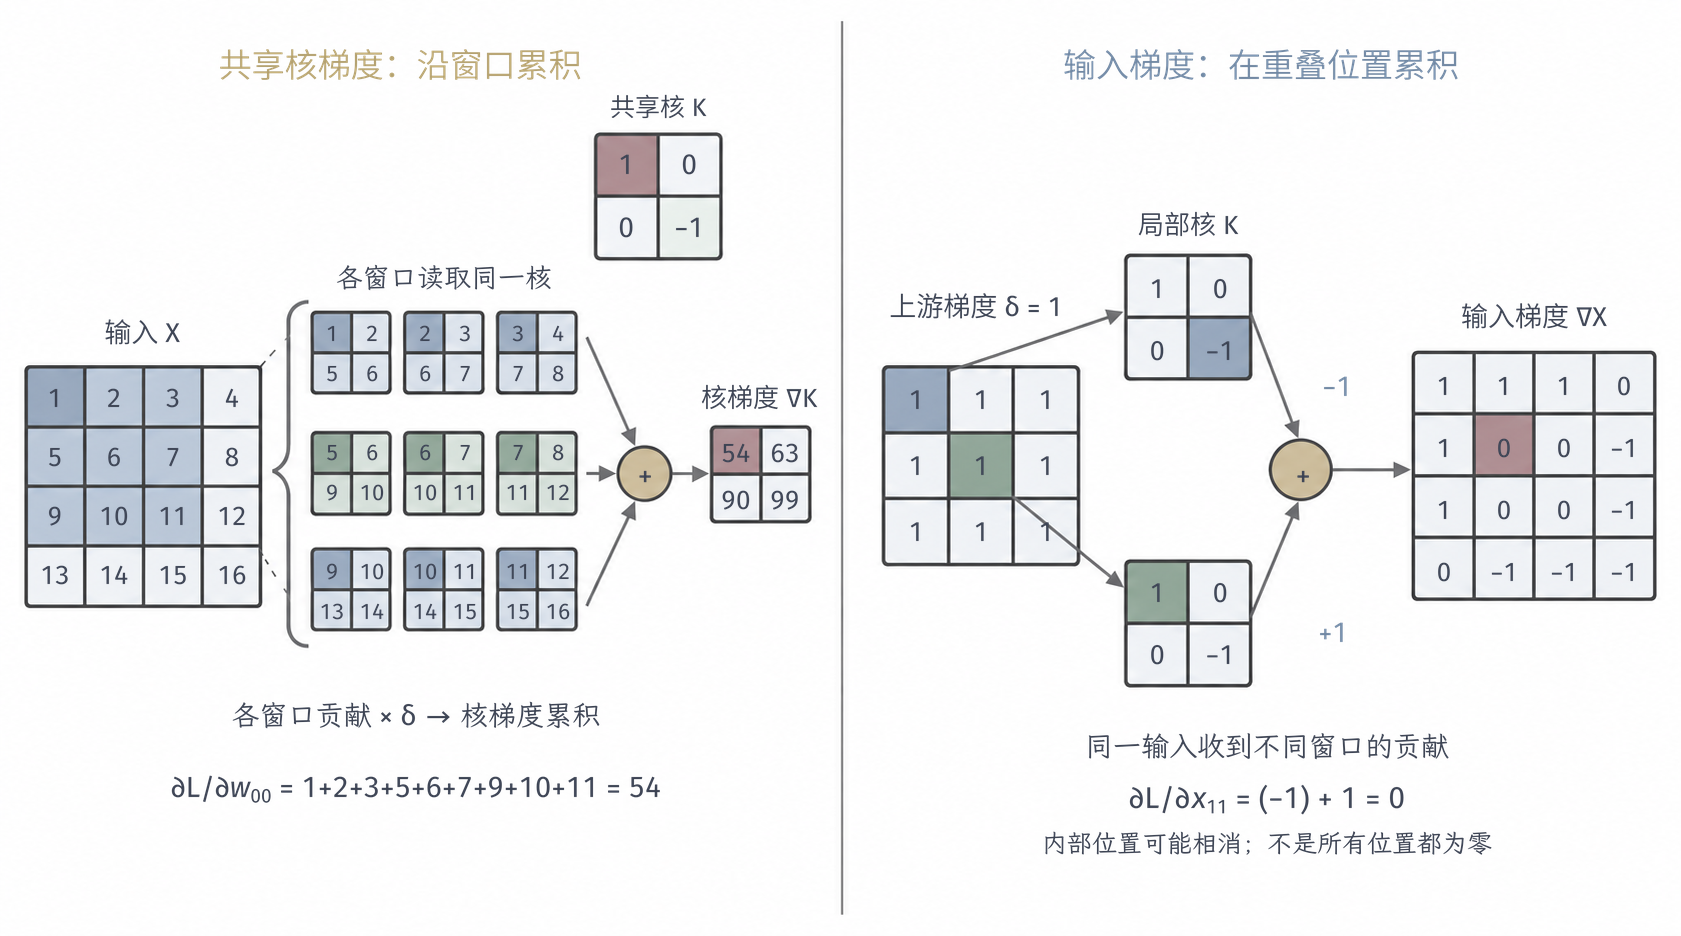
\includegraphics[width=142.325mm]{figures/05-neural-network-models/00-shared/generated/cnn-backprop-shared-overlap/figure.png}
  \caption{式~\eqref{eq:cnn-gradient-example}中的两种梯度累积。输入为按行排列$1$至$16$的$4\times4$矩阵，核为$(1,0;0,-1)$，步长一、无填充，损失为九个输出之和。左图汇总九个窗口对同一核参数的贡献；右图突出$x_{1,1}=6$的两项非零贡献，二者相消；另两项贡献因对应核值为零而为零。}
  \label{fig:cnn-backprop-shared-overlap}
\end{figure*}

\subsection{池化层反向传播}
\label{sec:cnn-pooling-backpropagation}

池化没有标准的可学习参数，但它决定上游梯度怎样返回输入。仍对完整批损失求导，设池化输出的梯度为$g_{t,i,j,c}=\partial L_B/\partial y_{t,i,j,c}$。平均池化对每个参与的元素具有相同导数，因此
\begin{equation}
  \frac{\partial L_B}{\partial x_{t,u,v,c}}
  =\sum_{i,j}\frac{g_{t,i,j,c}}{q_{i,j}}
                  \mathbb I\{(u,v)\in\Omega_{i,j}\}\text{。}
  \label{eq:cnn-average-pooling-gradient}
\end{equation}
分母必须与前向平均采用的计数相同。窗口重叠时，一个输入收到多项；全局平均池化则将某通道的上游梯度均分给该通道全部位置。

最大池化在最大值唯一时，只对被选中的元素有非零导数。前向计算记录其位置$(u^*_{t,i,j,c},v^*_{t,i,j,c})$，后向使用同一位置：
\begin{equation}
  \frac{\partial L_B}{\partial x_{t,u,v,c}}
  =\sum_{i,j}g_{t,i,j,c}
       \mathbb I\{(u,v)=(u^*_{t,i,j,c},v^*_{t,i,j,c})\}\text{。}
  \label{eq:cnn-max-pooling-gradient}
\end{equation}
若多个元素并列最大，函数在该点不可微；实现可以按固定规则选择一个位置，也可以采用最大值集合上的合法次梯度分配。后向采用与前向对应的选择或次梯度规则。同一元素若是多个重叠窗口的最大值，会收到这些窗口梯度的和。

对式\eqref{eq:cnn-pooling-example}，令四个输出梯度均为一。平均池化使每个输入收到$1/4$，最大池化只让原矩阵中的$6,8,14,16$各收到$1$。回传规则因此保留了两种汇聚方式的区别：平均把影响均分，最大把影响路由到当前胜出的位置。卷积与池化梯度接入前章的反向传播后，就能联合更新整个网络；优化器和学习率的通用选择由后续训练章讨论。

\section{卷积神经网络的扩展}
\label{sec:cnn-extensions}

\subsection{支持更深的网络结构}
\label{sec:cnn-deep-structures}

到VGG为止，增加深度的主要手段是不断串联卷积层。但实践中发现一个反直觉的现象：当网络从几十层继续加深时，\emph{训练误差不降反升}。这不能用过拟合解释——过拟合是训练误差很低、测试误差升高；这里连训练集上的误差都变差了，说明瓶颈在优化本身：层数过多后，梯度在长长的串联链路上反复相乘，深层参数难以获得有效的更新信号。这一现象称为\term{退化问题}（degradation problem），它发生在训练集上，是更深参数化带来的求解困难，而非单纯的泛化问题。ResNet论文在其图像实验中报告并研究了这一现象\scite{he2016resnet}

一个自然的破解思路是：\emph{不要强迫每一叠层都去重新构造完整的表示，而是允许信息“抄近道”直接绕过它们}。如果新加入的几层在当前任务上暂时没有用处，最理想的情况是它们能轻松地退化为“什么都不改”，网络的表现至少不应比更浅时更差。跨层连接正是提供这种近道的机制。下面比较三种组织方式：把旁路信息与变换结果直接\emph{相加}（残差连接）、用一个可学习的\emph{门}控制新旧信息的混合比例（Highway网络），以及把旧特征沿通道轴\emph{拼接}保留下来（密集连接）。它们都不形成有向环，因而仍是前馈网络，但各自改变了中间表示和梯度回传的路径。

\subsubsection{残差连接与ResNet}
\label{sec:cnn-resnet}

先看“让多余的层能轻松什么都不改”在数学上意味着什么。普通串联模块要把输入$\bm x$映射成目标输出$\bm y=\bm H(\bm x)$；若理想的$\bm H$恰好接近恒等（即这几层本可不改变输入），普通模块就必须\emph{主动学出}恒等映射$\bm H(\bm x)=\bm x$，而用一堆带非线性的卷积层精确凑出恒等相当困难。\term{残差连接}（residual connection）换了一个参数化：把输入直接加到变换分支的输出上，让这组层只需要学习“输出相对输入还差多少”。将输入特征展平为$\bm x\in\mathbb R^d$，维度相同时，模块写为
\begin{equation}
  \bm y=\bm x+\bm F_{\bm\theta}(\bm x)\text{。}
  \label{eq:cnn-residual-block}
\end{equation}
其中$\bm F_{\bm\theta}:\mathbb R^d\to\mathbb R^d$由若干卷积、归一化和激活组成。若目标映射接近恒等，残差分支只需接近零。这里的“残差”是模块输出相对于输入的差，不是标签减去预测值的训练误差。

图~\ref{fig:cnn-resnet}展开一个基本模块中的层与残差连接。上方旁路把输入直接送到加法节点，主分支则计算需要叠加的变换；图中的模块还在相加后施加一次ReLU。
\begin{figure*}[htbp]
  \centering
  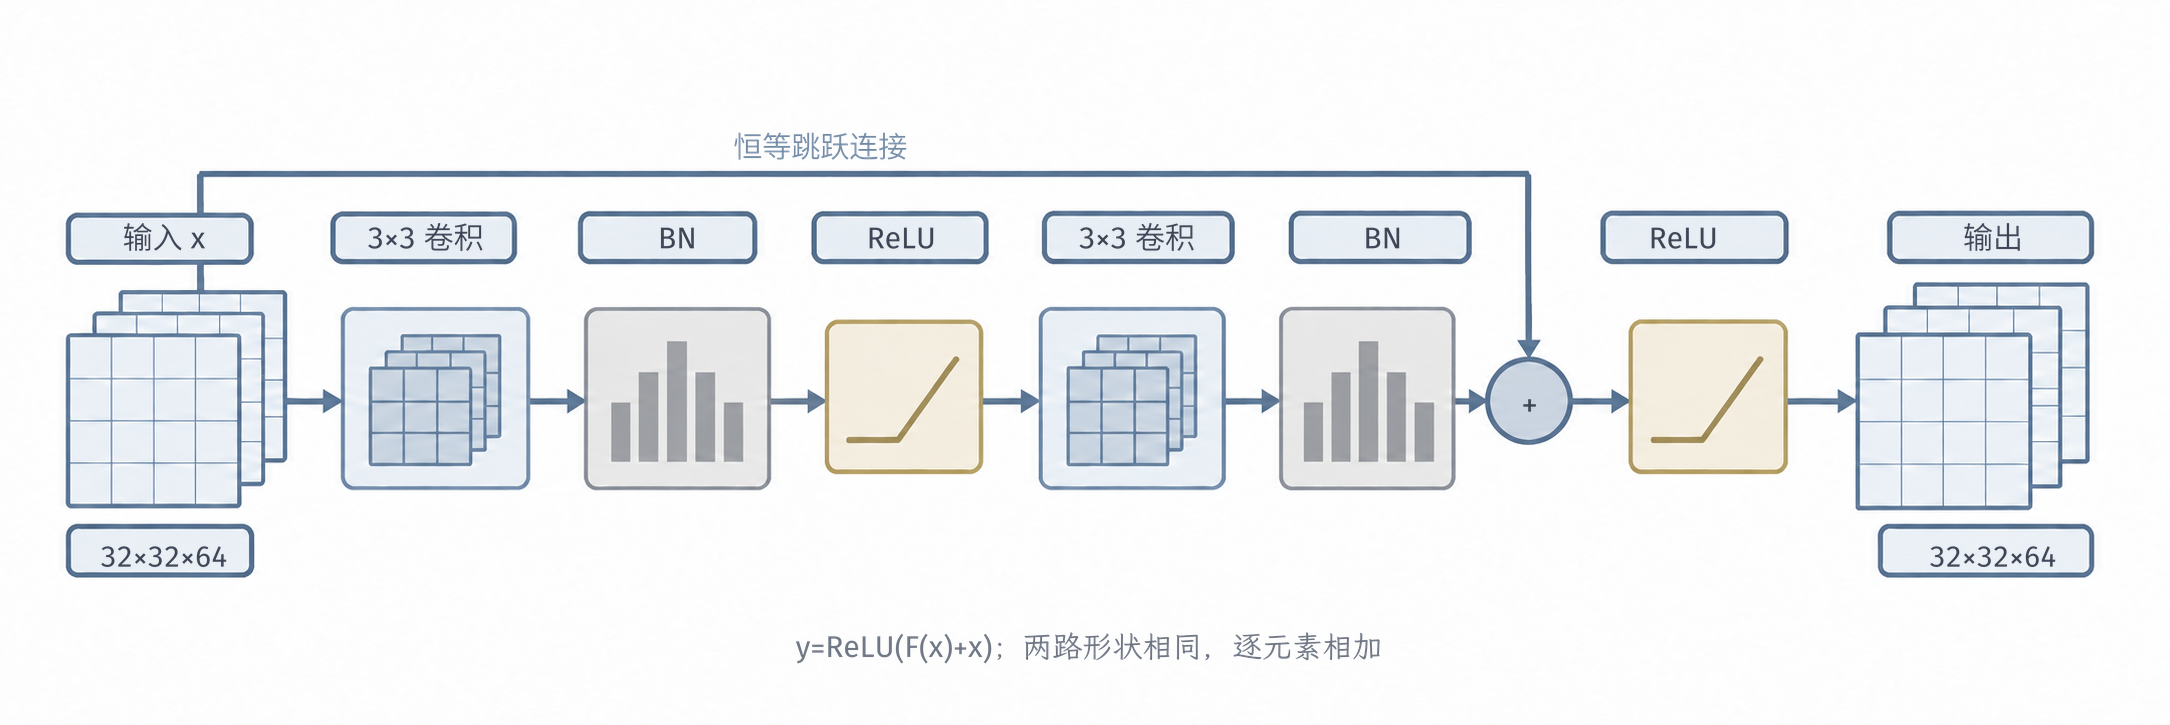
\includegraphics[width=169.000mm]{figures/05-neural-network-models/00-shared/generated/cnn-resnet/figure.png}
  \caption{残差基本模块中的逐层变换与恒等旁路。主分支依次经过$3\times3$卷积、BN、ReLU及第二个$3\times3$卷积、BN，再与直接传来的输入逐元素相加并激活。两次卷积均保持$32\times32\times64$形状，上方旁路跳过主分支的变换。圆角方框表示算子，圆形加号节点表示逐元素相加；改变尺度或通道时，旁路需要投影。}
  \label{fig:cnn-resnet}
\end{figure*}
下面只考察相加本身，暂不在相加后施加额外激活；含训练态BN时，$\bm x$应包含参与统计的整批特征。在可微位置，令$\bm J_F=\partial\bm F/\partial\bm x$。输入的微小变化$\mathrm d\bm x$沿两条路径分别产生$\mathrm d\bm x$与$\bm J_F\,\mathrm d\bm x$，相加后有
\[
  \mathrm d\bm y=\mathrm d\bm x+\bm J_F\,\mathrm d\bm x
    =(\bm I+\bm J_F)\,\mathrm d\bm x\text{。}
\]
对标量损失$\ell$，链式法则给出$\mathrm d\ell=(\nabla_{\bm y}\ell)^\top\mathrm d\bm y$。代入上式，再与$\mathrm d\ell=(\nabla_{\bm x}\ell)^\top\mathrm d\bm x$比较，就得到
\begin{equation}
  \begin{aligned}
    \frac{\partial\bm y}{\partial\bm x}&=\bm I+\bm J_F,\\
    \nabla_{\bm x}\ell&=(\bm I+\bm J_F)^\top\nabla_{\bm y}\ell\\
      &=\nabla_{\bm y}\ell+\bm J_F^\top\nabla_{\bm y}\ell\text{。}
  \end{aligned}
  \label{eq:cnn-residual-gradient}
\end{equation}
末行的第一项直接经过恒等路径，第二项经过残差分支。两项共同决定输入梯度，例如标量分支$F(x)=-x$就有$1+F'(x)=0$，两路贡献恰好相消。多块连乘后，尺度还随各块Jacobian矩阵变化；恒等路径改变了传播结构，整体梯度仍由全部路径决定。

若记相加结果为$\bm z=\bm x+\bm F(\bm x)$，再令$\bm y=\operatorname{ReLU}(\bm z)$，则反向还要先经过ReLU：
\[
  \nabla_{\bm x}\ell
    =(\bm I+\bm J_F)^\top\bm D_{\mathrm{ReLU}}\nabla_{\bm y}\ell\text{。}
\]
在$z_i\neq0$处，$\bm D_{\mathrm{ReLU}}$的第$i$个对角元素为$\mathbb I\{z_i>0\}$；零点按实现选定导数。这层激活也筛选恒等路径传来的贡献，相加结果与最终输出因而具有不同的导数。

当阶段间下采样或改变通道时，输入与分支结果不能直接逐元素相加。可用投影$\bm P$调整形状，写为$\bm y=\bm P\bm x+\bm F(\bm x)$；例如用跨步$1\times1$卷积同时改变空间尺寸与通道。此时跨层路径的Jacobian矩阵是$\bm P$，不再是$\bm I$，合并输出的Jacobian矩阵相应变为$\bm P+\bm J_F$。选择恒等或投影，取决于两条分支的形状和希望保留的映射。

ResNet在多个阶段堆叠残差模块。基本模块常用两个$3\times3$卷积；瓶颈模块用$1\times1$压缩通道、$3\times3$处理空间、再用$1\times1$恢复通道，以控制主体计算。经典版本在相加后使用激活。不同版本通过激活位置、旁路投影和下采样所在分支确定计算图；这些选择共同影响信息和梯度路径。

ResNet-18的主干分为四个阶段：对$224\times224$输入，前端$7\times7$卷积取步长二、填充三，产生$112\times112$特征；接BN、ReLU及$3\times3$、步长二、填充一的最大池化，得到$56\times56$网格。四个阶段分别使用64、128、256、512个通道，每个阶段包含两个基本模块；后三阶段的首模块将空间减半，并用投影匹配相加形状。末端全局平均池化与分类层完成整体读出。

\subsubsection{门控连接与Highway网络}
\label{sec:cnn-highway}

直接相加始终保留输入并叠加变换；若希望根据当前输入控制两条路径的比例，可以让网络学习一个门。\term{Highway网络}（Highway network）用控制门调节哪些坐标更多采用新变换、哪些更多保留原值。维度相同、保留门与变换门互补时，
\begin{equation}
  \begin{aligned}
    \bm g(\bm x)&=\operatorname{Sigmoid}(\bm G(\bm x)),\\
    \bm y&=\bm g(\bm x)\odot\bm F(\bm x)
            +(\bm1-\bm g(\bm x))\odot\bm x\text{。}
  \end{aligned}
  \label{eq:cnn-highway-block}
\end{equation}
其中$\bm F$为变换路径，$\bm G$产生与输入同形状的门得分，Sigmoid逐元素把门值限制在$(0,1)$。在卷积模块中，$\bm F$和$\bm G$都可使用共享局部计算。门值接近零时以保留路径为主，接近一时以变换路径为主。原工作采用负的门偏置，使初始门倾向保留输入，帮助很深的网络开始学习\scite{srivastava2015highway}

门值随输入变化，这一变化也参与输出导数。
在可微位置，先固定一个坐标$i$，将式\eqref{eq:cnn-highway-block}写成$y_i=g_iF_i+(1-g_i)x_i$；这里$g_i$和$F_i$都随整个输入$\bm x$变化。对两个乘积分别使用乘积法则，有
\[
  \begin{aligned}
    \mathrm d y_i
      &=g_i\,\mathrm d F_i+F_i\,\mathrm d g_i
        +(1-g_i)\,\mathrm d x_i-x_i\,\mathrm d g_i\\
      &=g_i\,\mathrm d F_i+(1-g_i)\,\mathrm d x_i
        +(F_i-x_i)\,\mathrm d g_i\text{。}
  \end{aligned}
\]
第一项记录变换结果的变化，第二项记录保留输入的变化，第三项合并了同一个门同时调整两条路径的影响。把所有坐标叠成向量，代入$\mathrm d\bm F=\bm J_F\,\mathrm d\bm x$和$\mathrm d\bm g=\bm J_g\,\mathrm d\bm x$，其中$\bm J_F=\partial\bm F/\partial\bm x$、$\bm J_g=\partial\bm g/\partial\bm x$，即可把每类逐坐标缩放写成一个对角矩阵。
记$\operatorname{Diag}(\bm v)$为以向量$\bm v$作对角线的矩阵，$\bm J_g$为门的Jacobian矩阵，则
\begin{equation}
  \begin{aligned}
    \bm J_y={}&\operatorname{Diag}(\bm g)\bm J_F
      +\operatorname{Diag}(\bm1-\bm g)\\
      &+\operatorname{Diag}(\bm F(\bm x)-\bm x)\bm J_g\text{。}
  \end{aligned}
  \label{eq:cnn-highway-gradient}
\end{equation}
末项来自门值随输入变化的影响。负偏置使门初始更接近保留路径，也可能让Sigmoid进入导数较小的区域，门参数的学习仍需合适尺度。Highway增加了可学习的路由及其参数成本；式\eqref{eq:cnn-highway-block}中两条系数之和为一，与ResNet无门控的直接相加具有不同约束。

图~\ref{fig:cnn-highway}展开变换、门和保留路径，两个逐元素乘法节点分别调节变换结果与原输入，再由相加节点合并。三条路径都保持$h\times w\times c$形状，门按位置和通道决定缩放系数；改变形状的模块还要为保留路径安排投影，并使门与两路结果具有匹配的目标形状。

\begin{figure*}[htb]
  \centering
  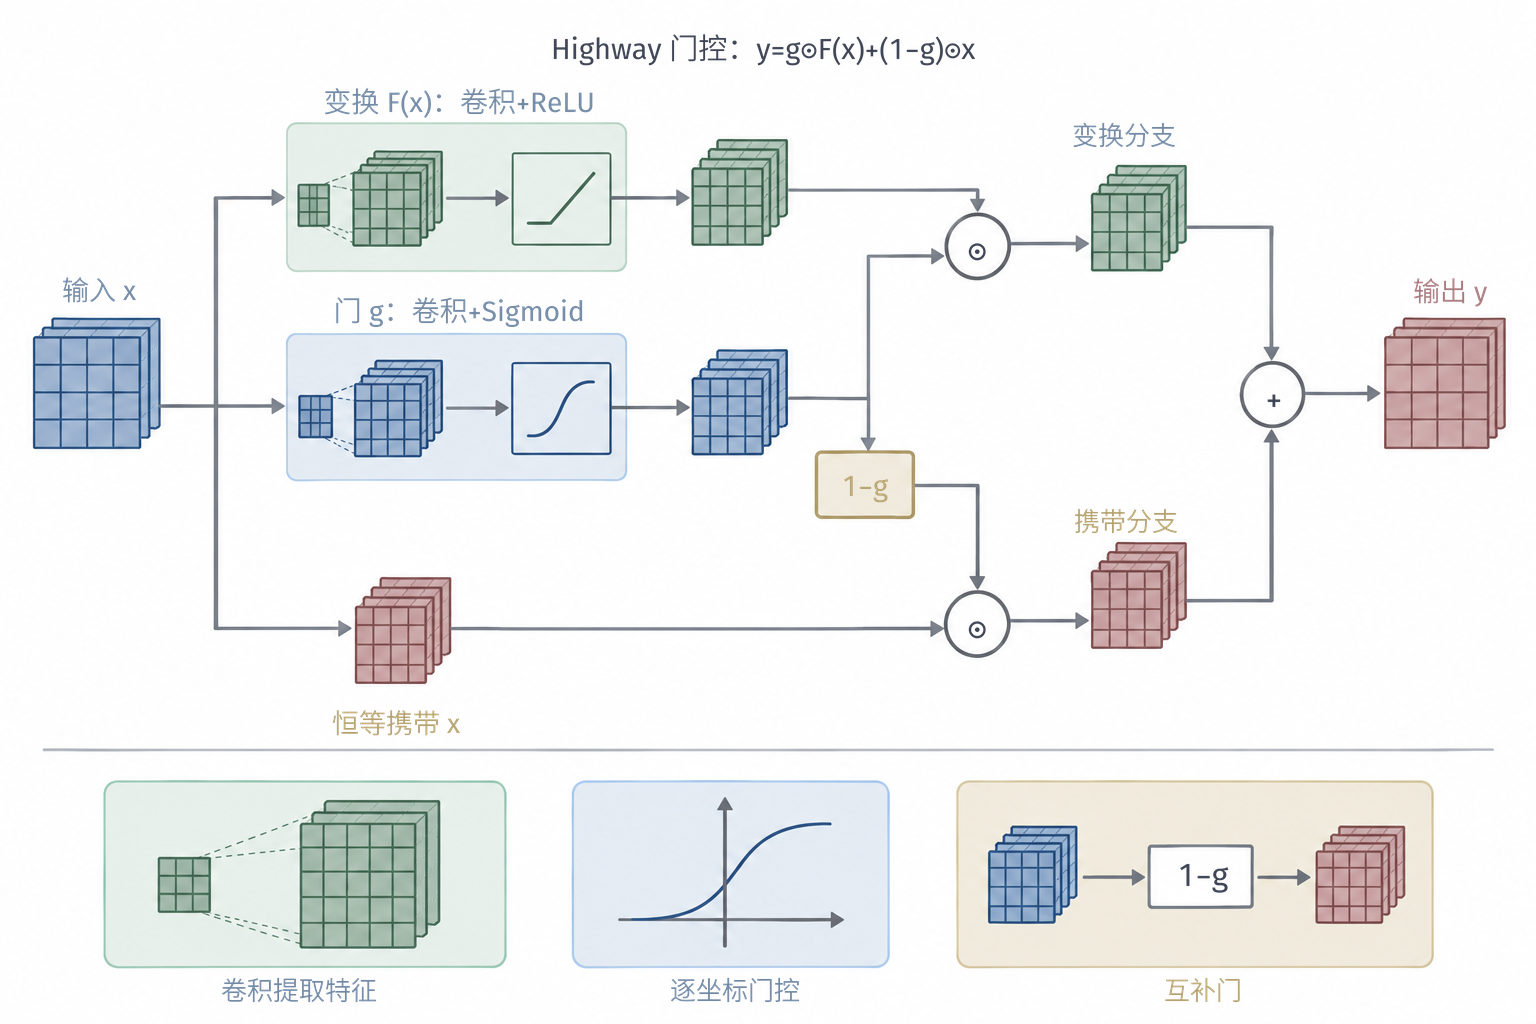
\includegraphics[width=130.048mm]{figures/05-neural-network-models/00-shared/generated/cnn-highway/figure.png}
  \caption{同形状卷积Highway模块。上方卷积与ReLU产生$\bm F(\bm x)$，门路径经卷积与Sigmoid产生$\bm g$，保留路径传递原输入；两个$\odot$节点分别计算$\bm g\odot\bm F(\bm x)$和$(\bm1-\bm g)\odot\bm x$，再由$+$节点相加。所有特征与门具有同一空间、通道形状，圆角方框表示各条路径的处理算子。}
  \label{fig:cnn-highway}
\end{figure*}
\FloatBarrier

\subsubsection{密集连接与DenseNet}
\label{sec:cnn-densenet}

残差相加把旧特征和新特征合在相同通道中。若希望后层仍能分别读取先前各层的特征，可以沿通道轴保留它们。\term{密集连接}（dense connection）使一个块内的每层读取全部先前层的输出；DenseNet按这种方式构造卷积模块：
\begin{equation}
  \bm H^{(\ell)}=\bm F_\ell\!\left(
      [\bm H^{(0)},\bm H^{(1)},\ldots,\bm H^{(\ell-1)}]
    \right)\text{。}
  \label{eq:cnn-dense-block}
\end{equation}
方括号表示通道拼接，不是逐元素相加；块内空间高、宽必须一致。$\bm H^{(0)}$为块的输入，各层只产生新的通道，旧特征仍可供更后层直接读取\scite{huang2017densenet}

若块输入有$c_0$个通道，每层新增$k$个通道，$k$称为\term{增长率}（growth rate），即每层增加的特征数。第$\ell$层输入有$c_0+(\ell-1)k$个通道，包含$L$层的整个块输出有$c_0+Lk$个通道。以$c_0=32,k=16,L=4$为例，各层依次读取$32,48,64,80$个通道，最终拼接得到$96$个通道。块间的\term{过渡层}（transition layer）用逐点卷积压缩通道，再通过池化降低空间尺寸，限制持续增长的特征规模。

密集连接提供直接的特征读取和梯度路径，但需要保留更多活动值。若每层只用一个产生$k$个新通道的$3\times3$卷积，忽略偏置，块内权重数为
\begin{equation}
  9k\sum_{\ell=1}^{L}\bigl(c_0+(\ell-1)k\bigr)
  =9k\left(Lc_0+\frac{kL(L-1)}2\right)\text{。}
  \label{eq:cnn-dense-cost}
\end{equation}
固定增长率下，这个简化块的通道相关成本随层数呈二次增长；瓶颈和压缩设计会改变具体成本。残差模块维持相加后的通道数，密集模块保留旧通道并增加新通道，二者以不同方式复用特征，活动值内存与计算量也由各自的通道增长和模块操作决定。


图~\ref{fig:cnn-densenet}从左向右展示一个三层教学密集块：32个初始通道加上三组16个新通道，输出为80个通道。每次变换前的全部特征经旁路保留，再与本层新产生的通道拼接，因而后层仍能读取每个先前层的输出。若在块后接过渡层，可用$1\times1$卷积把80个通道压缩为40个，再通过池化把$32\times32$空间网格缩为$16\times16$。

\begin{figure*}[htb]
  \centering
  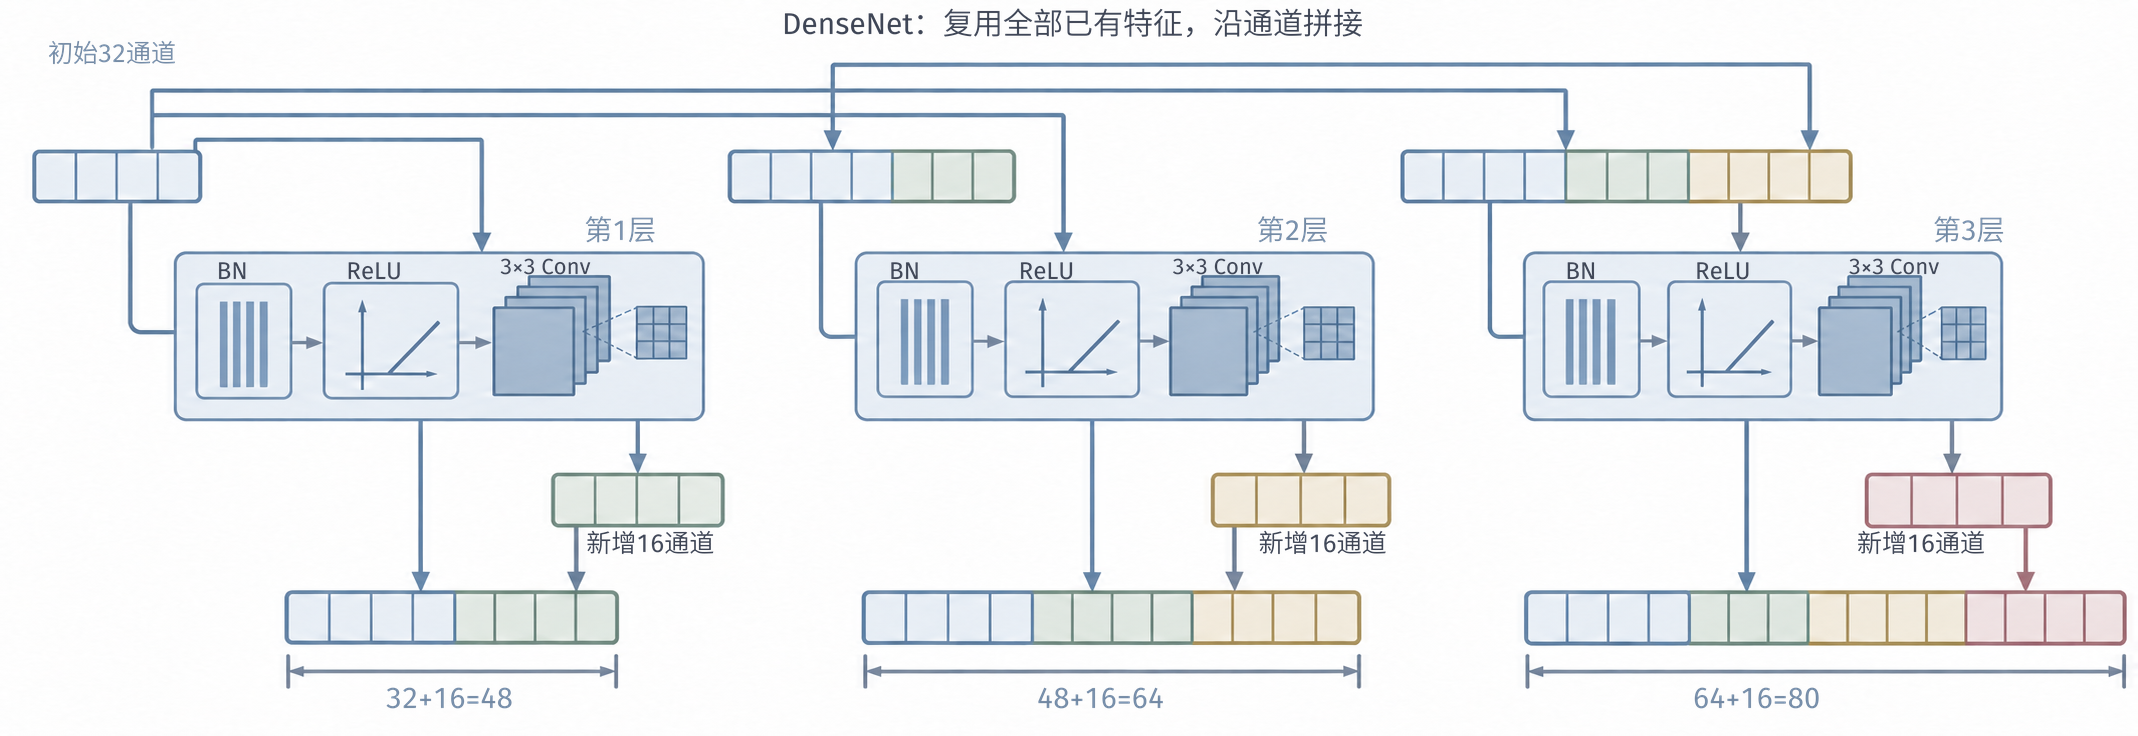
\includegraphics[width=169.000mm]{figures/05-neural-network-models/00-shared/generated/cnn-densenet/figure.png}
  \caption{DenseNet的三层教学密集块。各$\bm F_\ell$依次执行BN、ReLU和$3\times3$卷积，保持$32\times32$空间网格并新增16个通道。三次变换分别读取32、48、64个通道；上方旁路保留变换前的全部特征，标出的32、48、64为累计通道数；卷积下方的16为新增通道数。拼接位置将新旧特征沿通道合并，最终得到80个通道。逐次累积拼接等价于保留并向后传递全部先前层的输出，不作逐元素相加。}
  \label{fig:cnn-densenet}
\end{figure*}
\FloatBarrier

沿图中的第三次变换看，输入的64个通道由三部分组成：32个块输入通道、第一层新增的16个通道、第二层新增的16个通道。第三层同时读取这三组特征，但只输出自己的16个新通道；最终的80通道输出才把四组特征完整拼在一起。“读取64个通道”与“产生16个通道”分别描述该层的输入和输出，增长率只限制后者。后层可以学习重新组合旧特征，无须先在每一次相加中把旧特征与新特征合成一组。

保留旧特征也改变了反向传播的汇总位置。同一个早期特征可以同时被块内多个后层读取，损失沿这些读取路径返回的梯度，需要在这个早期特征处相加。拼接的反向操作则按通道切开输出梯度，把各段送回原来对应的特征。这些直接读取路径减少了某些梯度必须经过的串联变换数，但每条路径上的导数及其汇总仍由具体参数决定，不能据此保证梯度始终保持某个尺度。

过渡层负责结束这种持续保留。若用逐点卷积把80个通道压成40个，每个新通道都是原来80个通道的可学习组合；下一块收到的是这40组组合结果，已不再分别保留全部旧通道。随后的池化再减少空间位置。压缩比例与增长率因而需要一起选择：较小的增长率减慢块内通道增加，较强的压缩减少块间传递的特征，两者都影响后层能够读取哪些信息及其成本。

\FloatBarrier

\section{理论分析}
\label{sec:cnn-theory}

卷积、池化和跨层连接都是对候选函数施加的结构约束。约束带来了参数共享和计算效率，但任何约束都是双刃剑：它在符合数据规律时帮助学习，在不符合时则可能从根本上排除目标函数。与前章一样，本节严格区分三个不同层面的问题，避免用一个层面的结论替代另一个：\emph{表达能力}问这些结构约束是否还\textbf{允许}网络表示目标函数（结构会不会把需要的信息删掉）；\emph{收敛性}问共享参数下的梯度下降\textbf{能否}找到好参数；\emph{泛化性}问找到的参数在新图像上的\textbf{风险有多大}。泛化分析采用$n$个独立同分布训练样本及同分布测试样本，架构和参数约束在抽样前就固定；若约束是看过数据后才选择的，则还要额外计入选择代价。

\subsection{表达能力}
\label{sec:cnn-expressivity}

对卷积结构，表达能力问题有一个比全连接网络更尖锐的形式：局部连接、权值共享和下采样在利用规律的同时，也明确地\emph{丢弃}了某些信息。因此判断其表达能力，关键是看被丢弃的信息是否恰好是完成任务所必需的。如果目标是“在任何位置识别同一种平移后的图案”，局部共享与目标高度吻合；但如果任务要求不同位置必须使用不同规则（例如图像左上角和右下角的同样图案对应不同含义），共享结构就可能无法表达，除非额外提供位置特征或不同的读出方式。同样，固定大小的感受野之外的信息无法在该层直接参与判断，只有靠增加深度、加大核宽或引入全局读取来突破这一边界。

池化和下采样对表达能力的限制尤其直接：它们可能把两个\emph{不同}的输入映射成\emph{同一个}表示。一旦两个本应区分的类别被汇聚成了相同特征，后续无论再堆多少层、再怎么加宽，都只能给它们相同的输出，信息无法凭空恢复。因此一个卷积网络族的表达能力，同时取决于可学习参数和结构保留了哪些信息；位置、细节和长距离交互一旦被删除，扩大后续层也无法弥补这一限制。下面用两个定理分别从“保留信息时足够强”和“丢弃位置时必然失败”两个方向把这一点严格化。

\begin{theorem}[卷积网络保留像素时的连续目标逼近能力]
\label{thm:cnn-continuous-approximation}
固定有限图像尺寸，设展平输入的取值域$D\subset\mathbb R^d$为非空紧集。允许逐点卷积、ReLU、无下采样的特征保留，以及展平后的可变宽度全连接读出。对任意连续目标$g:D\to\mathbb R^q$和$\varepsilon>0$，这一卷积网络族包含$f$，使$\sup_{\bm x\in D}\lVert f(\bm x)-g(\bm x)\rVert_2<\varepsilon$。
\end{theorem}
\begin{proof}
逐点卷积为每个输入通道产生正、负两路，经ReLU得到$\rho(x_j)$与$\rho(-x_j)$。展平后可由两者之差恢复每个像素，后续全连接读出再应用定理~\ref{thm:ffn-continuous-approximation}。
具体地，若输入有$c$个通道，逐点卷积可在每个位置使用同一竖直拼接矩阵$[\bm I_c;-\bm I_c]\in\mathbb R^{2c\times c}$并取零偏置。将正、负两路按正路在前、负路在后的顺序展平为$\bm h(\bm x)=(\rho(\bm x),\rho(-\bm x))\in\mathbb R^{2d}$后，线性重构$[\bm I_d,-\bm I_d]\bm h(\bm x)=\bm x$逐坐标成立。若前章的逼近网络第一层为$\bm A\bm x+\bm b$，只需把读出首层权重设为$\bm A[\bm I_d,-\bm I_d]$，就能从保留的两路特征开始执行同一网络；因此重构可以并入读出的仿射层，不要求ReLU本身保留负值。
\end{proof}
该结论依赖保留位置及全部像素的读出，不能直接用于强制全局平均的架构。它给出了一个足够丰富的CNN候选族，不声称局部共享一定比全连接表示更省参数。

\begin{theorem}[平移不变卷积网络无法逼近位置判别目标]
\label{thm:cnn-position-obstruction}
设所有候选$f$在指定平移$\tau$下满足$f(\tau\bm X)=f(\bm X)$。若输入域同时包含$\bm X_0$与$\tau\bm X_0$，目标在两处分别取$0$与$1$，则
\[
 \inf_f\max\{|f(\bm X_0)|,\ |f(\tau\bm X_0)-1|\}\geq\tfrac12\text{。}
\]
\end{theorem}
两处候选输出相同，而任何实数不可能同时距$0$和$1$小于$1/2$。例如，同一个标记从左侧移到右侧时标签改变，严格平移不变的得分就无法逼近该目标。循环边界、步长一的等变卷积接全局平均是一种满足前提的结构；零填充边界和跨步会改变前提，需要对实际架构检查。

\subsection{收敛性}
\label{sec:cnn-convergence}

卷积核在多个位置复用，完整反向传播把各位置的梯度相加。权重共享不消除深层参数间的乘积，端到端目标通常仍非凸。若前向算子及损失连续、损失非负，并对全部参数加入正的二次惩罚，最小值存在；参数的通道交换等对称性通常妨碍唯一性。

\begin{theorem}[卷积网络光滑目标的驻点收敛速度]
\label{thm:cnn-stationary-rate}
固定训练集、网络结构和确定性的前向计算，记全批量训练目标为$J(\bm\theta)$。假设$J\geq J_{\inf}$，且梯度在包含迭代点及更新线段的区域内为$\beta$-Lipschitz，其中$\beta>0$。采用完整梯度下降
$\bm\theta^{(k+1)}=\bm\theta^{(k)}-\eta\nabla J(\bm\theta^{(k)})$，步长满足$0<\eta\leq1/\beta$。对任意$K\geq1$，
\begin{equation}
 \frac1K\sum_{k=0}^{K-1}\lVert\nabla J(\bm\theta^{(k)})\rVert_2^2
 \leq\frac{2[J(\bm\theta^{(0)})-J_{\inf}]}{\eta K}\text{。}
 \label{eq:cnn-stationarity-rate}
\end{equation}
对任意$\varepsilon>0$，至少有一个已计算迭代点的梯度范数不超过$\varepsilon$，只需
$K\geq2[J(\bm\theta^{(0)})-J_{\inf}]/(\eta\varepsilon^2)$。
\end{theorem}
证明与定理~\ref{thm:ffn-stationary-rate}相同：沿完整计算图求出梯度，使用下降引理并对更新次数求和。

该界回答了接近一阶驻点需要多少次更新。它不保证驻点是全局最小点，也不保证参数序列存在唯一极限。若还满足$\lVert\nabla J\rVert_2^2\geq2\mu(J-J_*)$，其中$\mu>0$、$J_*$为最小值，再限制$\eta\leq1/\mu$，则有
$J(\bm\theta^{(K)})-J_*\leq(1-\eta\mu)^K[J(\bm\theta^{(0)})-J_*]$。这一条件需要对具体训练问题验证，不能由网络名称推得。

光滑激活、固定填充与池化规则，以及确定性的前向计算，才可能满足定理的光滑假设；最大池化并列点、ReLU拐点和随机Dropout需要分别处理。共享、残差或密集连接本身不能推出全局最优的收敛速度。若只学习固定卷积特征上的岭读出，则具有与前馈网络相同的唯一解和线性收敛结论。
这里沿用定理~\ref{thm:ffn-readout-unique-rate}的条件：固定设计矩阵与平方损失，对全部读出权重施加系数$\lambda>0$的二次惩罚，并用目标Hessian最大特征值$L$确定步长$1/L$。若把偏置增广为一个常数特征，前章这一结论也将其计入被惩罚的读出权重。
输入尺寸、窗口重叠和各层尺度可能改变$\beta$，所以同一个$O(1/K)$阶数也可能对应不同的允许步长和每轮计算量。

\subsection{泛化性}
\label{sec:cnn-generalization}

前章泛化分析的核心思想是：真实风险与训练误差的差距由“候选函数空间有多大”来控制——空间越大，模型越容易在有限样本上偶然拟合，差距的上界就越宽。卷积结构最直接的好处正是\emph{用权值共享大幅压缩了候选空间}：同一个核在所有位置复用，自由参数远少于全连接网络，因此有望在更少样本上获得更紧的风险界。本节先把这一直观结论在一个最简单的“单共享核+全局平均”线性模型上\emph{算出具体数字}，再说明向深层CNN推广需要什么条件。全程以独立图像及其标签为样本：虽然一张图内部的像素高度相关、窗口彼此重叠，但样本数$n$计的是\emph{独立图像}的张数，不能把一张图里的大量像素当成大量独立样本。

要使用前章的复杂度工具，需要一个能刻画“这个卷积模型能产生多丰富的输出”的量。先构造这个受限模型。此处只研究单通道标量得分，省去激活和偏置，并在局部线性响应之后作全局平均。设展平输入为$\bm x\in\mathbb R^d$，第$r$个窗口的取数矩阵为$\bm P_r\in\mathbb R^{q\times d}$，共有$m$个窗口。
此处$q$是一个窗口按固定顺序展开后的长度。$\bm P_r$的每一行对应一个核位置：若该位置读取原输入的第$j$个坐标，这一行只在第$j$列取一，其余列为零；若该位置落在零填充区，这一行全部为零。因此，$\bm P_r\bm x$恰好按核的排列顺序列出第$r$个窗口的值。不同窗口可以读取同一个像素，窗口内则按下面的假设不重复取数。
采用零填充且每个窗口内不重复读取同一坐标，定义平均窗口向量
\begin{equation}
  \bm\phi(\bm X)=\frac1m\sum_{r=1}^{m}\bm P_r\bm x,
  \qquad f_{\bm w}(\bm X)=\bm w^\top\bm\phi(\bm X)\text{。}
  \label{eq:cnn-pooled-linear-model}
\end{equation}
其中$\bm w\in\mathbb R^q$为共享核权重。
第$r$个位置的局部线性响应为$\bm w^\top\bm P_r\bm x$。在$m$个位置取平均时，共享权重不随$r$改变，所以
\[
  \frac1m\sum_{r=1}^{m}\bm w^\top\bm P_r\bm x
  =\bm w^\top\left(\frac1m\sum_{r=1}^{m}\bm P_r\bm x\right)
  =\bm w^\top\bm\phi(\bm X)\text{。}
\]
这就把“局部响应后全局平均”的网络计算化成了平均窗口向量上的线性得分。

假设抽样前固定$\lVert\bm w\rVert_2\leq\alpha$，输入满足$\lVert\bm x\rVert_2\leq r_x$。取数不会增大单个窗口的范数，再由三角不等式有$\lVert\bm\phi(\bm X)\rVert_2\leq r_x$。
具体地，$\bm P_r\bm x$的平方范数只对被选中的不同输入坐标求平方和，补零行不增加这一和。因此
\[
  \lVert\bm\phi(\bm X)\rVert_2
  \leq\frac1m\sum_{r=1}^{m}\lVert\bm P_r\bm x\rVert_2
  \leq\frac1m\sum_{r=1}^{m}\lVert\bm x\rVert_2
  =\lVert\bm x\rVert_2\leq r_x\text{。}
\]
下面的风险界将用候选类的复杂度控制从训练风险推断期望风险所需的代价，因此先在当前核约束下计算这个量。

现在先固定已经观测到的训练样本$S=((\bm X_t,\bm Y_t))_{t=1}^{n}$；下面的复杂度计算只使用其中的输入，考察候选函数类$\mathcal H=\{f_{\bm w}:\lVert\bm w\rVert_2\leq\alpha\}$能够在这批输入上产生多大的随机起伏。这里$\alpha\geq0$，复杂度计算中的随机性来自另行生成的符号，而不是重新抽取图像。

要衡量一类函数“拟合任意标签的能力”，可以做一个思想实验：不给样本真实标签，而是随机抛硬币给每个样本派一个$+1$或$-1$的“假标签”。如果某个函数类足够丰富、能把这些毫无规律的随机标签也拟合得很好，说明它容量很大，在真实数据上也就更容易过拟合。具体地，给每个样本独立赋予一个符号$\varepsilon_t$，以相同概率取$-1$或$+1$。对一组固定符号，$n^{-1}\sum_t\varepsilon_t f(\bm X_t)$衡量候选得分与这组随机正负号的平均关联程度；再在$\mathcal H$中取上确界，表示允许为这组符号挑选关联最大的候选；最后对符号取期望，使结果不依赖某一次具体的抛硬币结果。这个量就是经验Rademacher复杂度——函数类对随机标签的最强平均拟合能力，其定义为
\[
  \widehat{\mathfrak R}_S(\mathcal H)
  =\frac1n\mathbb E_{\bm\varepsilon}
    \left[\sup_{f\in\mathcal H}
      \sum_{t=1}^{n}\varepsilon_t f(\bm X_t)\right]\text{。}
\]
注意它刻画的是\emph{整个受约束候选类}拟合随机符号的能力，而不是某个已经训练好的核；这个值越大，说明模型越容易记住噪声，泛化界越松。把当前线性得分代入这一定义，便可得到下面的范数表达式。
对独立随机符号$\varepsilon_t\in\{-1,+1\}$，经验Rademacher复杂度满足
\begin{equation}
  \begin{aligned}
    \widehat{\mathfrak R}_S(\mathcal H)
    &=\frac\alpha n\mathbb E_{\bm\varepsilon}
           \left\lVert\sum_{t=1}^{n}\varepsilon_t\bm\phi(\bm X_t)\right\rVert_2\\
    &\leq\frac\alpha n
         \sqrt{\sum_{t=1}^{n}\lVert\bm\phi(\bm X_t)\rVert_2^2}
     \leq\frac{\alpha r_x}{\sqrt n}\text{。}
  \end{aligned}
  \label{eq:cnn-pooled-rademacher}
\end{equation}
这里$\mathcal H$是满足该核约束的候选函数类。等号来自欧氏球上线性函数的最大值，第一条不等式来自均方根上界，交叉项因随机符号独立而消失。窗口数$m$没有显式出现，因为我们控制了平均后的特征范数；这不表示窗口产生了$m$倍独立样本。

为了逐步核对式\eqref{eq:cnn-pooled-rademacher}，对固定符号记$\bm v_{\bm\varepsilon}=\sum_t\varepsilon_t\bm\phi(\bm X_t)$。此时上确界中的和等于$\bm w^\top\bm v_{\bm\varepsilon}$。Cauchy--Schwarz不等式给出上界$\alpha\lVert\bm v_{\bm\varepsilon}\rVert_2$；当$\bm v_{\bm\varepsilon}\neq\bm0$时，取$\bm w=\alpha\bm v_{\bm\varepsilon}/\lVert\bm v_{\bm\varepsilon}\rVert_2$达到上界，当$\bm v_{\bm\varepsilon}=\bm0$时所有候选都给出零。这就得到了第一行的等号。

接着对非负随机量$\lVert\bm v_{\bm\varepsilon}\rVert_2$使用均值不超过均方根的关系：
\[
  \mathbb E_{\bm\varepsilon}\lVert\bm v_{\bm\varepsilon}\rVert_2
  \leq\sqrt{\mathbb E_{\bm\varepsilon}
                    \lVert\bm v_{\bm\varepsilon}\rVert_2^2}\text{。}
\]
展开根号内的平方范数，$t,u$分别遍历$n$个固定输入，得到
\[
  \begin{aligned}
    \mathbb E_{\bm\varepsilon}\lVert\bm v_{\bm\varepsilon}\rVert_2^2
      &=\sum_{t=1}^{n}\sum_{u=1}^{n}
        \mathbb E[\varepsilon_t\varepsilon_u]
        \langle\bm\phi(\bm X_t),\bm\phi(\bm X_u)\rangle\\
      &=\sum_{t=1}^{n}\lVert\bm\phi(\bm X_t)\rVert_2^2\text{。}
  \end{aligned}
\]
对角项使用$\varepsilon_t^2=1$；非对角项使用独立性与零均值，故$\mathbb E[\varepsilon_t\varepsilon_u]=0$。再将每项特征范数限制为$r_x$，平方和至多为$nr_x^2$，乘上外部因子$\alpha/n$便得到$\alpha r_x/\sqrt n$。

\begin{theorem}[核约束下线性卷积的期望风险界]
\label{thm:cnn-pooled-risk-bound}
对式\eqref{eq:cnn-pooled-linear-model}的模型族，设独立同分布的训练图像数为$n$，$\lVert\bm w\rVert_2\leq\alpha$、$\lVert\bm x\rVert_2\leq r_x$，这两个约束及架构在抽样前固定。设$\delta\in(0,1)$。若损失取值于$[0,1]$、对得分具有Lipschitz常数$\lambda_{\mathrm{loss}}$，并满足相应可测性条件，以至少$1-\delta$的概率，对全部上述模型有
\begin{equation}
  R(f)\leq\widehat R_S(f)
    +\frac{2\lambda_{\mathrm{loss}}\alpha r_x}{\sqrt n}
    +3\sqrt{\frac{\log(2/\delta)}{2n}}\text{。}
  \label{eq:cnn-pooled-risk-bound}
\end{equation}
\end{theorem}
其中$\delta\in(0,1)$为失效概率，$R$与$\widehat R_S$使用同一损失（风险界参考\BookTheoremRef{thm:rademacher-risk-bound}{卷3《基础、理论与可信性》第5章“二分类学习的可学习性”第5.4.3节“由Rademacher复杂度估计期望风险”}）。这个界针对受约束的线性共享核与有界Lipschitz损失，明确给出了样本数、输入尺度和核约束的作用。深层CNN或无界交叉熵改变了分析对象，需要另外建立复杂度与风险条件。若平均汇聚已经删掉标签需要的位置差异，复杂度很小的模型也可能具有较大的逼近误差。学习判断仍需结合式\eqref{eq:ffn-risk-decomposition}中的逼近、估计和优化三项。

深层CNN含非线性和多层结构，不能直接套用上面线性共享核的复杂度项。一个仍然能给出\emph{明确}结论的简单办法，是从“参数有多少种取值组合”的角度计数：如果把每个系数限制为有限个离散取值，那么整个网络的候选函数数量就是有限的，可以逐个套用有界损失的集中不等式，再用并合界同时控制。

\begin{theorem}[有限精度CNN在有界损失下的期望风险界]
\label{thm:cnn-quantized-risk}
固定CNN架构、图像范围、预处理和读出，共有$p$个可调系数；每个系数只取预先规定的至多$2^b$个值，其余配置固定。设损失在$[0,1]$内且可测，$S$含$n$个独立同分布图像样本。对任意$\delta\in(0,1)$，以至少$1-\delta$的概率，全部候选（因而任意训练输出$\widehat f$）满足
\[
 R(\widehat f)\leq\widehat R_S(\widehat f)
 +\sqrt{\frac{pb\log2+\log(2/\delta)}{2n}}\text{。}
\]
\end{theorem}
\begin{proof}
候选数至多为$2^{bp}$。对每个候选使用有界损失的Hoeffding不等式，再对全部候选作并合界，得到同时成立的双侧风险偏差界，取上侧即可。

将实际不同的候选函数组成集合$\mathcal F_{\mathrm{fin}}$，记其大小为$N$。每个参数最多有$2^b$种选择，$p$个参数的配置数至多为$(2^b)^p=2^{bp}$；不同配置还可能给出相同函数，所以$N\leq2^{bp}$。

对一个在抽样前固定的$f\in\mathcal F_{\mathrm{fin}}$，各样本损失$\ell(f(\bm X_t),\bm Y_t)$是独立同分布的$[0,1]$内随机量。经验风险是它们的均值，期望风险是同分布新样本上的损失期望。因此，对任意偏差阈值$\tau>0$，Hoeffding不等式给出
\[
  \mathbb P\!\left(
    |R(f)-\widehat R_S(f)|>\tau\right)
  \leq2\exp(-2n\tau^2)\text{。}
\]
为了让训练后选出的任一候选仍能使用这条界，需要控制全部候选中至少有一个失效的概率。将这$N$个失效事件的概率相加，并合界得到
\[
  \mathbb P\!\left(
    \exists f\in\mathcal F_{\mathrm{fin}}:
    |R(f)-\widehat R_S(f)|>\tau\right)
  \leq2N\exp(-2n\tau^2)\text{。}
\]
令右侧不超过$\delta$，对阈值解不等式，就得到
\[
  \tau\geq\sqrt{\frac{\log N+\log(2/\delta)}{2n}}\text{。}
\]
再用$\log N\leq pb\log2$选择定理中的阈值。以至少$1-\delta$的概率，全部候选的双侧偏差同时受控，其中上侧给出$R(f)\leq\widehat R_S(f)+\tau$。在这一事件上，不论训练怎样根据同一批数据从候选中选择$\widehat f$，它都已被同时覆盖，因而可以将$f$换成训练输出。
\end{proof}
这个界覆盖非线性、多层与共享结构，但通过参数存储量控制容量，通常较粗；数值超过1时只能给出平凡保证。若训练还选择了$M$种预先规定的架构，应在分子增加$\log M$。
这里要求$p$是这$M$种架构可调系数数目的共同上界，且每个系数都遵守相同的至多$2^b$取值约束；候选总数于是至多为$M2^{bp}$，取对数就增加$\log M$。若各架构的参数数目或取值数量不同，则先将各架构的候选数相加，再把总数的对数代入同一推导。
连续实数参数不满足有限候选前提，需另用参数覆盖或范数分析。原始交叉熵无界也不满足损失前提。参数共享减少$p$，却不能弥补读出丢失位置造成的表达限制；换设备、场景或图像分布时，同分布界亦需重新建立。

\section{常见应用}
\label{sec:cnn-applications}

前面的图像分类把整张图压缩成一个类别，输出不再保留位置。但还有一大类视觉任务要求输出\emph{一张与输入对齐的新图}：图像分割要给每个像素打标签，灰度着色要给每个像素填颜色。这类任务不能在最后用全局池化把位置信息抹平，而必须一边借助深层的大上下文判断“这是什么区域”，一边把输出分辨率恢复回来、使答案对准原位置。两类任务通常都采用\term{编码器—解码器}（encoder--decoder）结构：编码器像普通分类网络一样逐步下采样，把输入变成空间较粗但通道更丰富、语义更强的特征；解码器再逐步上采样恢复输出网格。这里的关键难题是：下采样和池化已经丢失了精细位置，解码器只靠粗糙特征无法还原锐利边界，必须另外安排细节的来源。

\subsection{图像分割}
\label{sec:cnn-segmentation}

图像分割为每个位置预测类别，例如在医学图像中逐像素区分不同组织区域。输入为$\bm X\in\mathbb R^{h\times w\times c_{\mathrm{in}}}$，目标标签矩阵为$\bm Y\in\{1,\ldots,q\}^{h\times w}$。这个任务同时需要两种信息：低层特征保留精细的边缘和纹理（决定轮廓落在哪里），高层特征结合大上下文判断区域身份（决定这一片是什么）。编码器越深、上下文越充分，但空间细节丢失越多；解码器需要把两者重新结合起来。

U-Net用从编码器到对应解码阶段的\term{跳跃连接}（skip connection）补充这些信息，即让较早的特征直接进入较后的计算。它在同一尺度上沿通道轴拼接编码特征与上采样后的解码特征，再用卷积融合。这里的跳跃连接沿通道保留两组特征，ResNet的残差连接则对匹配坐标求和；后续卷积读取的对象由此不同。原始U-Net采用不填充卷积，需要裁剪编码特征再拼接；本节教学版本采用保持尺寸的卷积，简化空间对齐\scite{ronneberger2015unet}

图~\ref{fig:cnn-encoder-decoder}将一个三尺度例子的编码、解码主路径按尺度分层排列，横向保留同尺度的跳跃连接。$64\times64$输入在最高分辨率产生$32$个通道，下采样到$32\times32$后产生$64$个通道，再到$16\times16$产生$128$个通道。解码器把低分辨率特征上采样，并与相同网格的编码特征拼接；卷积再将拼接结果整理为该尺度的输出通道。最终用$1\times1$卷积将每个位置的$32$维特征映射为$q$个类别得分。

\begin{figure*}[htb]
  \centering
  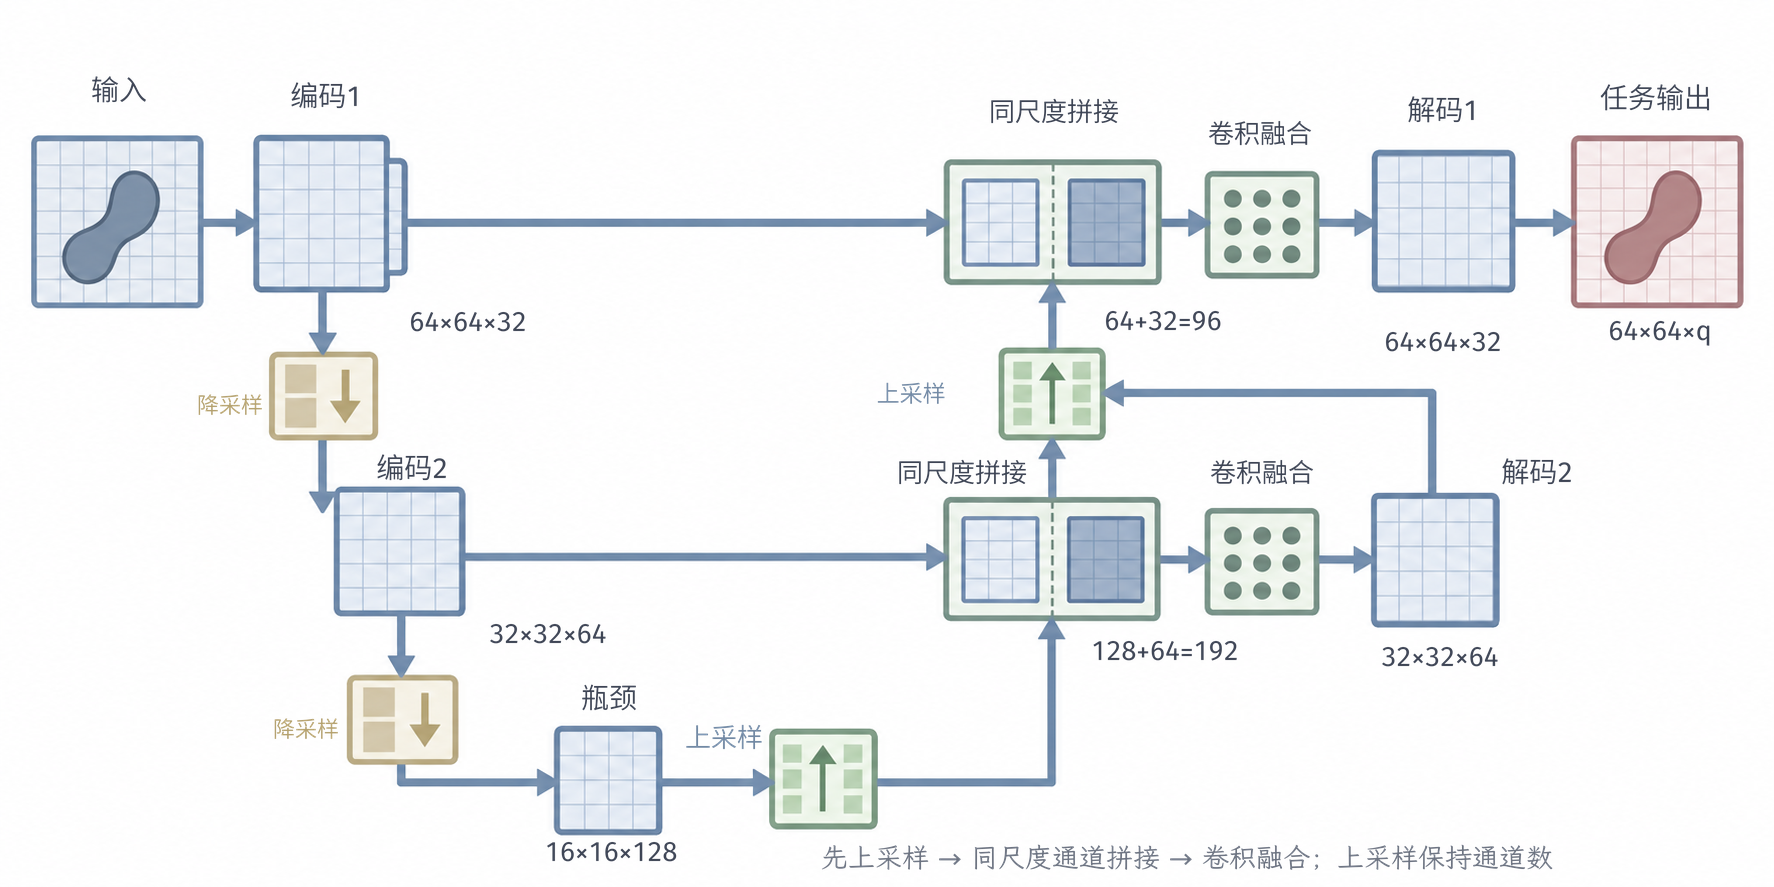
\includegraphics[width=150.199mm]{figures/05-neural-network-models/00-shared/generated/cnn-encoder-decoder/figure.png}
  \caption{用于分割或着色的三尺度编码器—解码器。平面特征片表示特征张量，标签给出空间尺寸和通道数。每级解码先上采样到下一尺度，再在同尺度拼接框中沿通道合并编码特征，随后卷积融合；横向跳跃连接均接入拼接节点。图中上采样保持通道数，因此两次拼接分别得到$128+64=192$和$64+32=96$个通道，卷积后变为64和32个。输出头产生$q$个类别得分或两个颜色通道；采用same卷积，省略原始U-Net的裁剪。}
  \label{fig:cnn-encoder-decoder}
\end{figure*}

跳跃连接为何有助于边界定位，可以从一次池化看出来。两个$2\times2$特征窗口分别只有左上角和右上角为一，其余位置为零；最大池化都输出一，粗网格上已无法据此区分响应原来在哪一侧。仅把这个一插值到更多位置，不能恢复已经舍去的区别。图~\ref{fig:cnn-encoder-decoder}中的横向连接把池化前仍保留位置的编码特征送到解码器，解码卷积便能把这些细节与较深层的上下文共同使用。是否形成正确边界还需要训练监督，连接本身只是提供原先缺少的信息来源。

\term{上采样}（upsampling）是增加网格分辨率的操作。可以先用最近邻或双线性插值生成更密的网格，再用普通卷积处理；也可以用转置卷积共同完成位置扩展与可学习变换。插值方式、目标尺寸和坐标对齐约定都要固定。输入高、宽若不能被总下采样倍数整除，可以在进入网络前填充、在输出后裁剪，或显式按目标尺寸上采样；拼接还要求两个空间轴对齐。

训练时，每张图像提供像素标签，网络按式\eqref{eq:cnn-segmentation-loss}计算损失，再联合更新编码器、解码器和输出头。未标注位置通过掩码排除；若少数类别被大量背景像素淹没，可以在明确权重和归一化后使用加权损失。推理时不需要标签，在各位置取最大得分类别，得到与目标网格对齐的分割图。像素准确率可能主要反映背景，因此评价还需按任务检查区域重叠和边界质量，具体指标在图像处理部分展开。

跨尺度连接把编码器仍保存的细节送给解码器。小目标能否保留，取决于输入分辨率和下采样过程；预测边界的监督又来自标注质量。解码层数、损失和连接方式需要与这些信息来源共同配置。

\FloatBarrier

\subsection{图像生成}
\label{sec:cnn-colorization}

分割的目标是离散类别，另一类空间输出任务则要在每个位置生成连续数值。灰度图着色就是一个直观例子：灰度图只提供亮暗信息，而同样亮度的区域可以对应完全不同的颜色，因此着色是一个\term{条件图像生成}（conditional image generation）问题——给定输入图像，生成一张与它相容的彩色图。本节沿用编码器—解码器，重点说明空间输出如何形成；同时也会暴露一个生成任务特有的困难：当同一个输入存在多种合理答案时，简单地最小化平均误差会得到“四不像”的平均结果。

采用Lab颜色表示时，一个通道描述亮度，另外两个通道描述颜色差异。把亮度按固定规则归一化为输入$\bm X\in\mathbb R^{h\times w\times1}$，将训练彩色图的两个颜色通道按预定尺度变为目标$\bm C\in\mathbb R^{h\times w\times2}$。编码器读取亮度中的边缘、纹理和上下文，解码器恢复颜色的空间分布，最后用$1\times1$卷积输出两个通道。若目标被缩放到$[-1,1]$，可以在输出使用Tanh；采用线性输出时，则需在转换与显示环节处理范围。归一化常数、反归一化和颜色空间转换必须一致，转成RGB后还要处理显示色域。

最直接的教学模型产生确定的颜色估计$\widehat{\bm C}=\bm f_{\bm\theta}(\bm X)$，用像素平方损失训练：
\begin{equation}
  \ell_{\mathrm{col}}=\frac1{hw}\sum_{i=0}^{h-1}\sum_{j=0}^{w-1}
      \lVert\widehat{\bm C}_{i,j,:}-\bm C_{i,j,:}\rVert_2^2\text{。}
  \label{eq:cnn-colorization-loss}
\end{equation}
分割与着色的主体可以采用相同的空间结构，但分割在每个位置输出类别概率，着色在这里输出两个连续值。使用时，将预测颜色反归一化，与输入亮度组合，再转换成彩色图像；模型不应无意中改变输入与输出的空间对齐。

平方损失还有一个与任务有关的限制。在颜色具有有限二阶矩且预测函数可自由选择时，条件平方损失的最优预测是$\mathbb E[\bm C\mid\bm X]$。若同一个灰度输入可能对应多种相距较远的颜色，平均值未必是一种合理着色；例如红与绿的平均可能降低饱和度。Zhang等将颜色空间离散成候选颜色，预测每个位置的颜色分布，用分类目标保留这种多解性，并讨论了平方损失的平均效应\scite{zhang2016colorization}

用一个简化的颜色坐标可以看清这种平均怎样产生。固定灰度输入和一个像素，假设其归一化颜色向量以相同概率取$(1,0)$或$(-1,0)$。确定性预测为$(t,s)$时，条件平均平方损失为$\tfrac12[(t-1)^2+s^2]+\tfrac12[(t+1)^2+s^2]=t^2+s^2+1$，在$(t,s)=(0,0)$处最小。这个最优预测处于两个可能颜色之间，却不是例子中任一种实际颜色。将输出改为候选颜色概率，才有可能分别保留这两种选择，而不是在训练目标中把它们合成一个平均值。

若把输出头改为$q_{\mathrm{col}}$个颜色得分，就可以逐位置归一化为候选颜色概率，再按约定选择、平均或采样得到颜色。各位置分别归一化给出局部候选概率，整张图像的空间协调还依赖它们之间的联合关系。若希望对同一输入生成多个整体协调的结果，还需要引入随机变量并设计相应的分布学习目标。本节的确定性模型把亮度、上下文和颜色估计连接起来；完整的条件生成还要建模同一亮度输入下多种协调颜色之间的分布。

\section{本章小结}
\label{sec:cnn-summary}

本章围绕开篇的问题——如何让网络保留空间结构并在多处复用同一识别规则——展开，可以收为五条主线。

第一，卷积网络用\textbf{局部连接}把每次计算限定在一个邻域内，用\textbf{参数共享}让同一组权重在所有位置复用，直接回应了全连接网络参数爆炸、无法平移复用的困难；多通道则让每个位置并行保存不同的局部特征。非线性激活与逐层组合把局部的边缘、纹理逐级拼成更大范围的判断。

第二，卷积这一运算由若干可独立调节的约定精确定义：数学卷积含核翻转而网络常用省略翻转的互相关；填充处理边界、步幅改变窗口间隔、空洞扩大核内采样间距、转置卷积则把局部贡献反向分配回去（用于上采样而非恢复信息）。明确这些约定，才能一致地计算输出尺寸、实现运算和推导梯度。

第三，计算算法与工程实现是两个层面：直接求和、矩阵化（im2col加GEMM）和Winograd、FFT等变换方法在精确算术下得到相同结果，却有不同的运算量、工作区和数值代价；分块、隐式GEMM、间接卷积和算子融合则进一步改变存储复用与访存。

第四，共享结构决定了梯度的两种累加：同一核权重在各位置的贡献要沿位置累加，一个输入在各重叠窗口的贡献要沿窗口累加；链式法则通过前向映射的转置把输出梯度分配回输入。残差相加、Highway门控和DenseNet拼接则为超深网络提供了不同的信息和梯度近道，以缓解退化问题，同时带来各自的通道规模与内存成本。

第五，结构约束是双刃剑：它在数据符合规则网格、局部相关和平移重复等假设时提升样本效率，但池化和不变性读出一旦删除了任务所需的位置信息，再大的网络也无法恢复；预测的可靠性仍取决于结构是否保留目标信息、样本是否提供足够的独立证据，以及优化能否得到合理解。分割与着色把这些要点综合起来：编码器构造大上下文，解码器恢复空间输出，跳跃连接把下采样前的细节送回去，而输出头和损失决定最终答案表示的是类别、连续值还是不确定性。

\paragraph{扩展阅读}
Goodfellow等教材第9章进一步讨论卷积、共享与池化的结构假设\scite{goodfellow2016}。早期文档识别中的实际配置可结合第~\ref{sec:cnn-lenet}节的LeNet-5与原论文阅读，注意边界、降采样及读出方式怎样配合任务。

\chapter{循环神经网络}
\label{chap:recurrent-networks}

先看两类需要“记住过去”的任务。判断“这部电影并不精彩”的情感时，否定词“并不”与几步之后的“精彩”必须联系起来，孤立看任何一个词都会得出相反结论；预测设备下一时刻的温度，也往往要依据此前一段时间的升降趋势，而不只是当前读数。这类任务有两个共同特征：输入是\emph{陆续到达}的（一个词接一个词、一个时刻接一个时刻），而且序列长度\emph{可以变化}（评论有长有短）。第~\ref{chap:feedforward-networks}章的前馈网络要求输入是固定维度、一次性全部给出；第~\ref{chap:convolutional-networks}章的卷积虽然能处理网格，但固定层数和核尺寸只对应有限的历史窗口。于是本章要回答：\emph{当输入陆续到达、长度可变时，网络怎样把历史中有用的信息带到当前，又怎样从当前的错误反过来学会调整此前的处理}？

解决思路是引入一个随时间不断更新的内部变量——隐状态。它像一张“便签”：每读入一个新输入，就结合便签上原有的摘要和新内容，把便签改写一遍；做预测时只看这张便签即可，而不必保留所有历史输入。任务读出从便签形成当前预测，训练则根据当前误差去调整“改写便签”的规则。这一思路立刻引出三个贯穿全章、且彼此独立的问题：其一，\emph{信息}问题——便签容量有限，它是否真的容纳了任务所需的远期信息；其二，\emph{学习}问题——当错误在很晚才暴露时，梯度能否穿过许多次改写、传回负责记下远期信息的早期参数；其三，\emph{代价}问题——整段处理与逐步处理、保存全部历史与只维护定长状态，在计算和存储上各有什么取舍。

本章沿“历史经由隐状态传递”这一条共同机制展开。先用最普通的循环网络给出完整的递推、读出和训练过程（\ref{sec:rnn-basic}节）；随后看到普通网络难以保存远期信息，于是依次出现几种不同的改造思路：储备池干脆\emph{固定}状态动态、只学读出（\ref{sec:rnn-reservoir}节），LSTM、GRU用可学习的门\emph{选择性地}保存和覆盖（\ref{sec:rnn-gated}节），注意力不再把全部历史压进一个末状态、而是\emph{保存各位置表示}按需读取（\ref{sec:rnn-attention}节），状态空间模型则从线性递推与卷积、扫描的代数等价出发，改变历史的\emph{计算组织}（\ref{sec:rnn-state-space}节）。之后讨论双向、树结构等拓扑和深度扩展（\ref{sec:rnn-extensions}节），并在\ref{sec:rnn-theory}节从理论上区分表达、优化与泛化。需要提醒的是，这里的“时间步”不必是物理时间，也可以是词的位置、扫描次序或有向结构中的计算顺序。

\FloatBarrier
\section{循环神经网络概述}
\label{sec:rnn-overview}

在正式定义循环网络之前，先体会一下“不用记忆”时最直接的做法及其局限。要预测下一时刻，最简单的办法是把最近若干个观测拼成一个固定长度的向量，交给前馈网络。这个滑动窗口确实包含了顺序，却有两个硬伤：窗口以外的信息完全无法影响预测（无论多早发生的关键事件都被截断），而且改变窗口长度就要改变输入层的参数规模，网络结构随之变动。时间卷积用共享卷积核有所改善，但固定层数和核尺寸仍只对应一个有限的历史窗口，无法自然地“同一套计算一直运行下去”。我们真正想要的是：\emph{一个能随每个新输入持续更新、并把历史影响传递下去的内部变量}——这样无论序列多长，网络本身的参数和规模都不需要改变。

这个变量就是\term{隐状态}（hidden state）：它是网络根据已读输入逐步形成的内部摘要，不是训练样本直接给出的标签。设输入序列为$\bm{x}_1,\ldots,\bm{x}_T$，其中$\bm{x}_t\in\mathbb{R}^{d}$，长度$T$可以随样本改变。用$\bm{h}^{(t)}\in\mathbb{R}^{m}$表示读完第$t$个输入后的状态，\term{循环神经网络}（recurrent neural network, RNN）通过状态反馈，把前一步的内部表示用于下一步计算：
\begin{equation}
  \bm{h}^{(t)}=F_{\bm{\theta}}\!\left(\bm{h}^{(t-1)},\bm{x}_t\right),
  \qquad t=1,\ldots,T\text{。}
  \label{eq:rnn-general-recurrence}
\end{equation}
这里$F_{\bm{\theta}}$是具有参数$\bm{\theta}$的更新函数，$\bm{h}^{(0)}$是初始状态。下标$t$标识序列中的输入，上标$(t)$标识状态更新的步数；它们在本章按同一步对齐。状态的具体内容由更新函数和任务学习决定，可以是影响情感的否定，也可以是温度趋势；这条递推式只规定新状态从何处获得信息。

同一组$\bm{\theta}$在不同时间步复用，称为时间方向的\term{参数共享}（parameter sharing）。因此，延长序列会增加更新次数，却不必增加循环单元的参数量。\term{时间展开}（unrolling through time）则把这些更新依次画成计算图：第$t$步读取已经得到的第$t-1$步状态，展开图按已计算的旧状态逐步求值，形成有序的时间链。图~\ref{fig:rnn-unrolling}将状态反馈和展开图对应起来；展开后的深度随$T$增长，也是长序列训练困难的来源。

\begin{figure*}[htb]
  \centering
  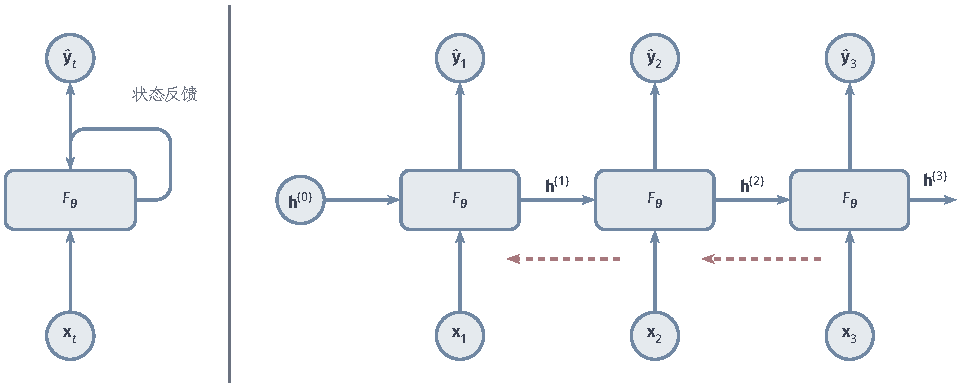
\includegraphics[width=162.810mm]{figures/05-neural-network-models/00-shared/tikz/rnn-unrolling/figure.pdf}
  \caption{状态递推的紧凑表示与时间展开。当前输入进入更新函数，隐状态沿时间传递，任务读出从状态形成预测。展开图中的$F_{\bm{\theta}}$是同一个更新函数的多次调用，参数共享而状态值不同。红色虚线示意较晚损失沿状态依赖回传梯度；图中只画三个更新步。}
  \label{fig:rnn-unrolling}
\end{figure*}
\FloatBarrier

循环网络的发展围绕两件事展开：怎样形成历史表示，以及怎样学到有用的状态更新。Elman在1990年的简单循环网络中，把前一步隐藏活动送回下一步，展示了这种上下文表示如何随序列任务形成。反馈在展开后成为一条时间链，同一参数因而可以作用于不同位置\scite{elman1990}

历史影响传到远处输出时，训练误差也要经过相应的多步依赖回传。Bengio、Simard和Frasconi在1994年分析了梯度学习与长期保留之间的困难：误差经多步状态变换回传时，影响可能迅速衰减或放大。这把研究重点从“网络是否含有反馈”推进到“反馈路径怎样传递信息与梯度”\scite{bengio1994rnn}

1997年的LSTM为持续记忆安排了单独的加性路径，后来加入的遗忘门使网络能够清除不再相关的内容。这条记忆通路与其他循环参数一起由任务目标训练。2001年的ESN和2002年的LSM则采用另一种分工：先构造通常固定的动态储备池，再学习任务读出。前一条路线让网络学习如何保存，后一条路线先提供历史特征；各自的原始工作和结构差别在第~\ref{sec:rnn-gated}节与第~\ref{sec:rnn-reservoir}节展开。

序列任务也推动了输出组织的变化。2014年，编码器—解码器使用一套循环网络读取源序列，另一套网络生成目标序列；Sutskever等用多层LSTM展示了这种端到端学习方式\scite{sutskever2014seq2seq} 同年的GRU用较少的门组织状态更新。随后，Bahdanau与Luong等的循环注意力模型让每个生成步骤重新读取编码器各位置的表示，减轻全部输入只能挤入同一末状态的限制。控制门改变保存方式，注意力改变读取方式，二者可以同时使用。

较新的状态空间路线还关心整段序列的计算组织。2020年的HiPPO把历史记忆写成在线投影问题；S4利用相应结构矩阵和快速核生成，在递推与卷积之间切换。2023年的Mamba把部分系数改为由输入产生，再通过选择性扫描计算；同年的RWKV以内容权重、时间衰减与定长累积量组织历史。第~\ref{sec:rnn-state-space}节将分别说明这些设计的原始形式。这些模型仍维护随输入更新的状态，并分别为状态构造、内容读取和计算执行安排结构。

本章按历史经由隐状态传递这一共同机制组织内容：链式循环、树递归、储备池以及基于隐状态递推的状态空间网络都在这里讨论。具体文献可能把状态空间网络单列为一类；各模型的具体更新函数和可训练参数在对应小节中另行给出。时间步也不必是物理时间，可以表示词的位置、扫描位置或有向结构中的计算次序。

\FloatBarrier
\section{基础循环神经网络}
\label{sec:rnn-basic}

本节先建立一个最普通的循环预测器，它由三组计算组成：\emph{状态更新}负责把新输入和旧状态概括成新状态，\emph{任务读出}规定在哪些位置、从状态产生什么预测，\emph{损失}衡量预测与目标的差距。理解这一节的关键是：同一套状态更新可以配不同的读出方式——可以只读最后一个状态给整段分类，也可以在每个位置都读出一个标签，还可以用两套网络在长度不等的序列之间转换。下面先给出共同的更新单元，再逐一介绍这些读出。

\subsection{网络结构}
\label{sec:rnn-structure}

普通RNN的更新规则非常直接：把当前输入和上一步状态各自线性映射后相加，再通过一个非线性函数。采用列向量约定，令
\begin{equation}
  \begin{aligned}
    \bm{z}^{(t)}&=\bm{U}\bm{x}_t+\bm{W}\bm{h}^{(t-1)}+\bm{b},\\
    \bm{h}^{(t)}&=\tanh\!\left(\bm{z}^{(t)}\right),\\
    \bm{a}^{(t)}&=\bm{V}\bm{h}^{(t)}+\bm{c},\qquad
    \widehat{\bm{y}}_t=g\!\left(\bm{a}^{(t)}\right)\text{。}
  \end{aligned}
  \label{eq:rnn-basic-cell}
\end{equation}
其中$\bm{U}\in\mathbb{R}^{m\times d}$决定新输入写入什么，$\bm{W}\in\mathbb{R}^{m\times m}$决定旧状态保留和混合多少，$\bm{b}\in\mathbb{R}^{m}$是隐藏偏置；$\bm{V}\in\mathbb{R}^{q\times m}$和$\bm{c}\in\mathbb{R}^{q}$从状态产生$q$维输出得分。这里用Tanh把状态限制在$(-1,1)$，既提供非线性又防止状态在反复递推中无界增大；它也可替换为其他激活，但梯度和状态范围会随之改变。$g$按任务选择恒等映射、Sigmoid或Softmax，输出与损失的配合沿用第~\ref{sec:ffn-output-objectives}节。

这里可以第一次看清循环网络为什么能用\emph{固定数量的参数}处理\emph{任意长度}的序列：$\bm U,\bm W,\bm b,\bm V,\bm c$这些参数与$T$完全无关，无论序列有多长，都只是反复套用同一个更新规则。代价则是计算必须按时间顺序进行——第$t$步依赖第$t-1$步的状态，天然难以并行。

这个单元及读出共有$md+m^2+m+qm+q$个参数，忽略逐坐标运算后，一步稠密计算的乘加量为$O(md+m^2+qm)$。长度为$T$的前向计算重复$T$次。固定宽度时，逐步预测只需维护当前状态；完整反向传播还需要沿途激活，或在求导时重算它们；保存这些激活时，训练存储随展开长度增加。

\subsubsection{序列到分类}
\label{sec:rnn-sequence-classification}

第一种读出对应“整段输入只有一个答案”的任务，如判断一整段评论是好评还是差评。网络把可变长度的评论逐步读入，但只在读完最后一个有效词后输出一次，因此称为\term{序列到分类}（sequence classification）。最直接的读出使用末状态：
\begin{equation}
  \bm{p}=\operatorname{softmax}\!\left(\bm{V}\bm{h}^{(T)}+\bm{c}\right),
  \qquad \ell=-\log p_y\text{，}
  \label{eq:rnn-classification}
\end{equation}
其中类别数为$K$、$q=K$、真实标签为$y\in\{1,\ldots,K\}$。末状态必须把与类别有关的信息带到结尾，所以较早出现的证据也要经过后续更新。

另一种读出对状态聚合，例如用$\overline{\bm{h}}=T^{-1}\sum_{t=1}^{T}\bm{h}^{(t)}$替代末状态。这里聚合的是已含历史的状态，仍然可以体现顺序；但平均会稀释只出现在少数位置的证据。末状态集中保留递推后的历史，平均分散各位置的影响，最大池化突出局部强响应，可学习聚合则按目标调整权重。标签依赖哪些位置，决定了这些读出各自需要保留的证据。


图~\ref{fig:rnn-sequence-classification}显示了末状态分类的监督位置：只有读完有效序列后，分类头才形成整段预测。
\begin{figure}[htb]
  \centering
  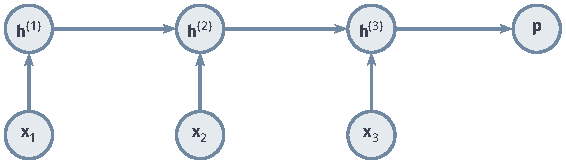
\includegraphics[width=95.793mm]{figures/05-neural-network-models/00-shared/tikz/rnn-sequence-classification/figure.pdf}
  \caption{序列到分类。三个输入依次更新同一循环单元，末状态产生类别概率$\bm p$。输入、隐状态与任务输出分列展示；图中只示意长度为3的序列。}
  \label{fig:rnn-sequence-classification}
\end{figure}
\FloatBarrier

\subsubsection{同步序列到序列}
\label{sec:rnn-aligned-sequences}

第二种读出对应“每个输入位置都要一个答案”，且输入与输出一一对齐，如给句子中每个词标注词性。\term{同步序列到序列}（aligned sequence-to-sequence）在每个有效位置都接上读出并计算损失：
\begin{equation}
  \ell=\frac{1}{T}\sum_{t=1}^{T}
  \ell_t\!\left(g(\bm{V}\bm{h}^{(t)}+\bm{c}),y_t\right)\text{。}
  \label{eq:rnn-aligned-loss}
\end{equation}
单向状态$\bm{h}^{(t)}$只读取$\bm{x}_1,\ldots,\bm{x}_t$。实时预测可以按这个可见范围运行。若任务允许读取整段输入，可以使用第~\ref{sec:rnn-topologies}节的双向结构补充后文信息。

时间预测也可以按位置组织，但要注明输出的时间含义。例如读入$\bm{x}_t$后预测$\bm{x}_{t+1}$，计算索引仍是$t$，目标却是下一步观测。这里的对齐指每个输入位置都接一个预测；目标的物理时刻由任务另外指定。


图~\ref{fig:rnn-aligned-sequences}在各位置设置读出；它与末状态分类共享同一种状态递推，但各位置都可以收到监督。
\begin{figure}[htb]
  \centering
  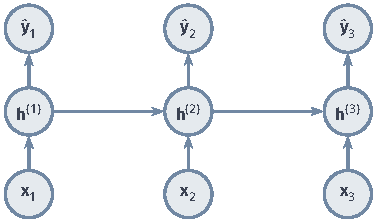
\includegraphics[width=63.793mm]{figures/05-neural-network-models/00-shared/tikz/rnn-aligned-sequences/figure.pdf}
  \caption{同步序列到序列。每个输入位置形成一个隐状态和相应预测。输入位置与预测位置对齐；若用于下一时刻预测，应另将目标移到后一时刻。图中单向状态只读取当前及此前输入。}
  \label{fig:rnn-aligned-sequences}
\end{figure}
\FloatBarrier

\subsubsection{异步序列到序列}
\label{sec:rnn-encoder-decoder}

第三种情形更一般：输出序列与输入序列\emph{长度不同、也没有天然的逐位置对应}，典型如机器翻译（一个英文词可能对应多个中文词、语序还要调整）。这时无法在每个输入位置上直接挂一个对齐的输出。\term{编码器—解码器}（encoder--decoder）把“读懂输入”和“产生输出”拆成两套循环网络：编码器先把整段输入读成一个上下文，解码器以此为条件，逐个生成目标符号。设目标长度为$S$，目标符号来自大小为$K$的词表，约定词表包含起止符号BOS和EOS。

解码器要把离散符号转换成向量输入，因此为每个符号保存一个$d_e$维的可学习向量，并将它们排成嵌入矩阵$\bm{E}\in\mathbb{R}^{d_e\times K}$。若$y$是符号的词表索引，\term{符号嵌入}（symbol embedding）就是查表取出的那一列，即$\bm{e}(y)=\bm{E}_{:,y}$；索引只用于选列，其数值大小不表示符号间的距离。用$\bm{s}^{(j)}$表示解码状态，基本形式为
\begin{equation}
  \begin{aligned}
    \bm{c}_{\mathrm{enc}}&=\bm{h}^{(T)},\qquad
    \bm{s}^{(0)}=\psi(\bm{c}_{\mathrm{enc}}),\\
    \bm{s}^{(j)}&=F_{\mathrm{dec}}\!\left(
      \bm{s}^{(j-1)},\bm{e}(y_{j-1}),\bm{c}_{\mathrm{enc}}\right),\\
    \bm{p}^{(j)}&=\operatorname{softmax}\!\left(
      \bm{V}_{\mathrm{dec}}\bm{s}^{(j)}+\bm{b}_{\mathrm{dec}}\right)\text{。}
  \end{aligned}
  \label{eq:rnn-encoder-decoder}
\end{equation}
$\psi$将编码状态映射到解码状态空间，编码器与解码器可以使用不同参数和宽度。起始符号$y_0=\mathrm{BOS}$为第一步提供输入，终止符号$\mathrm{EOS}$表示生成结束；它们也有各自的嵌入列。下文把$y_S=\mathrm{EOS}$计入目标序列。使用真实前缀训练时，$y_{j-1}$来自目标序列；生成时，它来自上一步概率分布中选出或采样的符号。两种情况都先查表得到$\bm{e}(y_{j-1})$再输入解码器；概率分布用于产生符号，符号索引用于取嵌入列。嵌入矩阵与其他网络参数一起通过训练更新。

目标序列的条件概率按生成次序分解：
\begin{equation}
  \begin{aligned}
    p_{\bm{\theta}}(y_{1:S}\mid\bm{x}_{1:T})
      &=\prod_{j=1}^{S}p_{\bm{\theta}}
        (y_j\mid y_{0:j-1},\bm{x}_{1:T}),\\
    \ell&=-\sum_{j=1}^{S}\log p^{(j)}_{y_j}\text{。}
  \end{aligned}
  \label{eq:rnn-sequence-likelihood}
\end{equation}
这里$y_{1:S}$、$\bm{x}_{1:T}$简记相应序列。条件中保留了此前目标，所以概率分解没有假设目标位置互相独立。对损失求和或按$S$平均，会分别让长序列包含更多损失项或先把各序列归一化，因而改变样本权重。

图~\ref{fig:rnn-encoder-decoder}将读取源序列与生成目标分开。两侧各画三个有效位置以便比较，并不要求实际源序列与目标序列等长。
\FloatBarrier
\begin{figure*}[t]
  \centering
  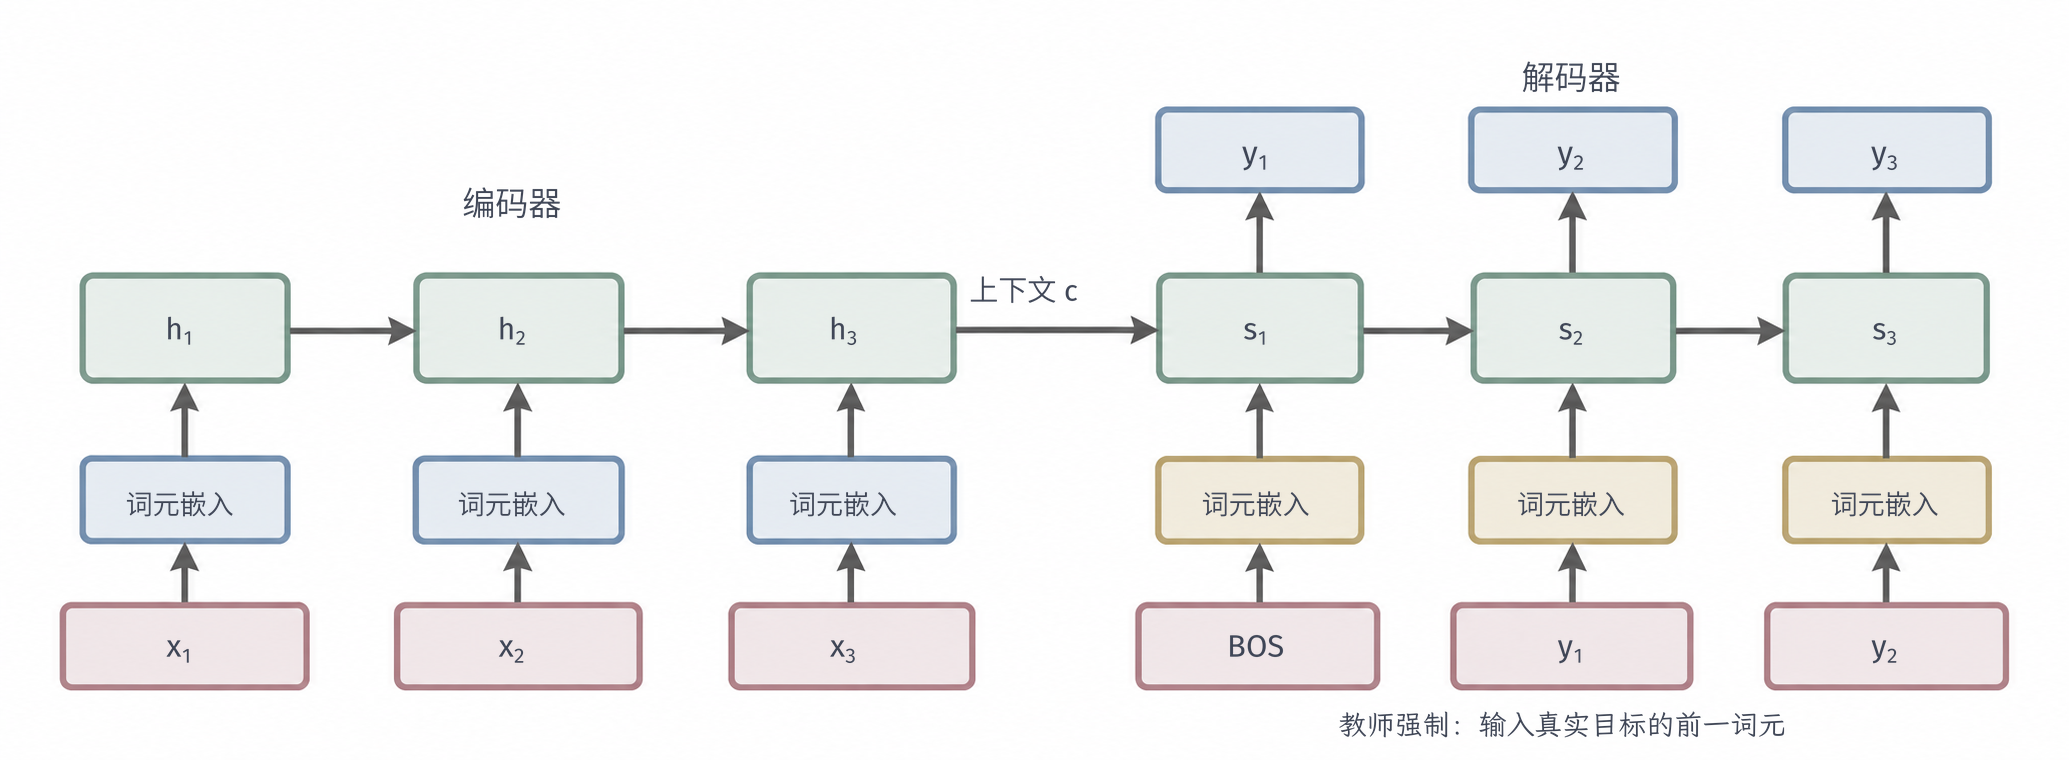
\includegraphics[width=169.000mm]{figures/05-neural-network-models/00-shared/generated/rnn-encoder-decoder/figure.png}
  \caption{异步序列到序列。编码器读取三个源输入，解码器在初态$\bm s^{(0)}$之后生成三个目标。BOS启动生成，右移后的目标经嵌入进入后续解码步。训练可使用真实目标，预测使用已生成目标；图中省略每步重复读取的固定上下文。}
  \label{fig:rnn-encoder-decoder}
\end{figure*}
\FloatBarrier

\subsection{参数学习}
\label{sec:rnn-learning}

循环网络的训练有两个区别于前馈网络的要点。第一，同一组参数在每个时间步都被使用，因此某个参数对总损失的影响，是它在\emph{所有时间步}上影响的总和，梯度必须沿时间累加。第二，循环矩阵$\bm W$被反复相乘，初始化时除了单步方差，还要关注多步连乘后信号是否被保持；正交初始化使初始的线性状态变换保持向量的欧氏范数，正是为了让信号在起点处既不快速放大也不快速缩小（激活导数仍会参与完整传播）。输入映射$\bm U$和输出映射$\bm V$可沿用第~\ref{sec:ffn-initialization}节的尺度原则。

状态的起点也要交代清楚。独立序列通常从一个固定的零状态，或同一个可学习的初始状态开始；若初态可学习，它的梯度同样由反向传播得到。在连续数据流上可以让状态跨批次延续，但前提是批次的每一行延续的是\emph{同一条}数据流；一旦换成无关样本，就必须重置状态。把上一条独立样本（比如上一篇评论）的隐状态带入下一条，等于让当前预测看到了不该看到的前文，会改变预测条件。

下面分别处理四个训练问题：怎样汇总共享参数在各时间步的梯度，怎样在长序列上控制存储和更新步长，怎样训练需要把输出反馈回来的序列模型，以及怎样维持跨很多步的梯度传播。前两项适用于一般循环训练；输出反馈取决于具体任务，长期依赖则需要进一步考察状态更新的动态。

\subsubsection{梯度计算与参数共享}
\label{sec:rnn-bptt}

循环网络带有“反馈环”，无法直接套用前馈网络逐层求导。一个关键技巧是\emph{时间展开}：把同一个更新函数在$T$个时间步上的调用依次画成一条首尾相连的长链——每一步都是一个“层”，相邻步之间传递状态。展开之后，它在数学上就等价于一个权重在各层之间\emph{共享}的很深的前馈网络，于是可以直接使用前两章的链式法则。这种沿时间展开图从后向前计算导数的方法，称为\term{随时间反向传播}（backpropagation through time, BPTT）。

以下以式\eqref{eq:rnn-basic-cell}为对象，令单序列目标为$L=\sum_{t=1}^{T}\ell_t$；没有监督的位置取$\ell_t=0$。记$\bm{g}^{(t)}=\partial\ell_t/\partial\bm{a}^{(t)}$，总损失对状态的梯度为$\bm{r}^{(t)}$，对预激活的梯度为$\bm{\delta}^{(t)}$，则
\begin{equation}
  \begin{aligned}
    \bm{r}^{(t)}&=\bm{V}^{\top}\bm{g}^{(t)}
       +\bm{W}^{\top}\bm{\delta}^{(t+1)},\\
    \bm{\delta}^{(t)}&=\bm{r}^{(t)}\odot
      \left(\bm{1}-\bm{h}^{(t)}\odot\bm{h}^{(t)}\right),
      \qquad \bm{\delta}^{(T+1)}=\bm{0}\text{。}
  \end{aligned}
  \label{eq:rnn-backward-recursion}
\end{equation}
$\odot$表示逐元素乘法。第一项来自当前读出，第二项来自后续状态；即使当前没有标签，后续损失仍可通过第二项监督这一步。若只在末状态分类，$t<T$的$\bm{g}^{(t)}$均为零，但相应$\bm{\delta}^{(t)}$未必为零。

每次调用都对共享参数产生一个局部贡献。求这一局部贡献时，将该步读入的上一状态视为独立输入；跨步依赖已由$\bm{\delta}^{(t)}$汇总，当前局部外积据此只计算本次调用对参数的影响。把所有调用的贡献累积起来，得到
\begin{equation}
  \begin{aligned}
    \nabla_{\bm{U}}L&=\sum_{t=1}^{T}\bm{\delta}^{(t)}\bm{x}_t^{\top},
    &\nabla_{\bm{W}}L&=\sum_{t=1}^{T}\bm{\delta}^{(t)}
      (\bm{h}^{(t-1)})^{\top},\\
    \nabla_{\bm{b}}L&=\sum_{t=1}^{T}\bm{\delta}^{(t)},
    &\nabla_{\bm{V}}L&=\sum_{t=1}^{T}\bm{g}^{(t)}(\bm{h}^{(t)})^{\top},\\
    \nabla_{\bm{c}}L&=\sum_{t=1}^{T}\bm{g}^{(t)},
    &\nabla_{\bm{h}^{(0)}}L&=\bm{W}^{\top}\bm{\delta}^{(1)}\text{。}
  \end{aligned}
  \label{eq:rnn-shared-gradients}
\end{equation}
这些梯度的形状与相应参数一致。自动微分沿所有调用位置汇总导数；这些位置共用一组参数，各步贡献更新的是同一对象。若目标按时间平均，相应梯度还需除以有效长度。

\begin{figure}[htbp]
  \centering
  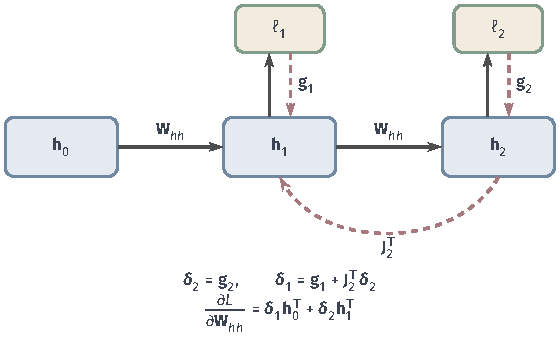
\includegraphics[width=94.756mm]{figures/05-neural-network-models/00-shared/tikz/rnn-bptt-two-steps/figure.pdf}
  \caption{两时间步BPTT的显式展开。蓝色实线是共享$\bm W_{hh}$的前向调用，红色虚线从$\ell_2$与$\ell_1$回传并在$\bm\delta_1$处汇合；同一循环矩阵的梯度等于两个调用位置的外积贡献之和。底部指出长序列中状态Jacobian连乘是梯度消失或爆炸的直接来源。}
  \label{fig:rnn-bptt-two-steps}
\end{figure}
\FloatBarrier

\begin{example}[两步递推中的梯度累积]
  \label{ex:rnn-shared-gradient}
  为单独观察共享参数，暂把Tanh换成恒等映射，使用标量更新$h^{(t)}=w h^{(t-1)}+x_t$；$w$是矩阵$\bm W$的一维情形。取固定初始状态$h^{(0)}=1$、$x_1=1$、$x_2=0$、$w=1/2$，只在末步计算损失$L=(h^{(2)})^2/2$。两次前向调用为
  \[
    \begin{aligned}
      h^{(1)}&=\tfrac12\times1+1=\tfrac32,\\
      h^{(2)}&=\tfrac12\times\tfrac32+0=\tfrac34\text{。}
    \end{aligned}
  \]
  反向从$r^{(2)}=h^{(2)}=3/4$开始，再沿第二步的状态依赖得到$r^{(1)}=w r^{(2)}=3/8$。本例激活导数为一，故$\delta^{(t)}=r^{(t)}$。第二次调用对$w$的局部导数是$h^{(1)}$，第一次是$h^{(0)}$，所以共享参数收到两项贡献：
  \[
    \begin{aligned}
      \frac{\mathrm dL}{\mathrm dw}
        &=r^{(1)}h^{(0)}+r^{(2)}h^{(1)}\\
        &=\tfrac38\times1+\tfrac34\times\tfrac32
          =\tfrac38+\tfrac98=\tfrac32\text{。}
    \end{aligned}
  \]
  第一项对应依赖路径$w\to h^{(1)}\to h^{(2)}\to L$，第二项对应$w\to h^{(2)}\to L$；梯度沿这些依赖逆向回传。两条路径的贡献最终相加，更新的仍是同一个$w$。直接展开$h^{(2)}=w(w+1)=w^2+w$，也有$\mathrm dL/\mathrm dw=(w^2+w)(2w+1)=3/2$，可与反向递推核对。

  若改取$h^{(0)}=0$，第一步对$w$的贡献为零，原因是$w$所乘的初态为零；共享参数仍在这一位置使用。若将本例的$h^{(0)}=1$改为可学习初态，它收到的梯度为$w r^{(1)}=3/16$，与$w$的梯度分开更新。
\end{example}

\subsubsection{长序列训练中的存储与更新控制}
\label{sec:rnn-truncation}

\paragraph{用截断限制反向传播的存储。}

长序列的完整展开会占用大量训练存储。\term{截断随时间反向传播}（truncated BPTT）把数据流分成有限长度的片段，在片段边界保留状态数值，却切断对更早计算的求导依赖。保留的状态数值仍把此前历史带入当前预测，求导则仅经过当前片段的更新。截断缩小了反向图，前向记忆仍由递推动态决定；遗漏跨边界路径后，所得梯度通常是完整梯度的有偏近似。

\paragraph{用裁剪限制过大的梯度。}

梯度过大时，可以在优化器更新之前使用\term{梯度裁剪}（gradient clipping），把梯度范数限制在阈值内。将全部参数梯度拼成$\bm{g}$，阈值为$\tau>0$，全局范数裁剪写为
\begin{equation}
  \widetilde{\bm{g}}=
  \begin{cases}
    \bm{g},&\lVert\bm{g}\rVert_2\leq\tau,\\
    \tau\bm{g}/\lVert\bm{g}\rVert_2,&\lVert\bm{g}\rVert_2>\tau\text{。}
  \end{cases}
  \label{eq:rnn-gradient-clipping}
\end{equation}
\Needspace{10\baselineskip}
对使用固定学习率的普通梯度下降，它保持非零梯度的方向并限制步长尺度，可减少异常大梯度造成的更新幅度。若学习率为$\eta>0$，参数增量为$\Delta\bm{\theta}=-\eta\widetilde{\bm{g}}$，故$\lVert\Delta\bm{\theta}\rVert_2=\eta\lVert\widetilde{\bm{g}}\rVert_2\leq\eta\tau$。对其他优化器，实际参数步幅还需结合其更新规则判断；式\eqref{eq:rnn-gradient-clipping}直接限制的是送入优化器的梯度范数。裁剪作用于已算出的参数梯度，早期影响若已衰减仍需从传播路径处理，前向状态动态也保持原定义。Pascanu等从状态Jacobian矩阵的乘积分析这两类梯度问题，并研究了裁剪的作用\scite{pascanu2013}

\paragraph{按样本边界与有效长度管理状态。}

可变长度批次常用填充补齐。\term{掩码}（mask）标记哪些位置是真实数据，使填充位置不参与损失或状态聚合。末状态读出使用每个样本的有效末位置；继续读取填充值会产生额外状态更新。平均聚合只汇聚有效位置，并以其数量作分母。

\subsubsection{自回归序列的训练与预测}
\label{sec:rnn-teacher-forcing}

这里出现一个训练与预测的不对称，是序列生成特有的关键问题。式\eqref{eq:rnn-sequence-likelihood}的条件概率默认每一步都以\emph{真实的}历史符号为前提；训练时确实可以把真实的$y_{j-1}$直接喂给第$j$步，这种做法称为\term{教师强制}（teacher forcing）：相当于老师在学生每写一个词时，都把正确的上文摆在他面前，让他专心学习“给定正确上文时下一个词该是什么”。但真正预测时并没有真实目标可用，第$j$步只能输入模型\emph{自己上一步生成}的符号；一旦早期生成错了，错误的前缀会把后续状态也带偏。于是训练时见到的前缀分布（总是正确）与预测时见到的前缀分布（可能含有错误）不一致，这种暴露偏差可能累积放大。

教师强制能直接、高效地优化真实序列的条件似然，因此仍是主流训练方式。若在训练中混入模型自己生成的符号，就改变了所学前缀的分布，需要相应地按新的生成过程建立学习目标，而不能简单套用。生成质量最终要在实际逐步预测的过程中评价：贪心解码每步选概率最大的符号；束搜索则同时保留若干个最有希望的候选前缀，但它覆盖的只是搜索空间的一部分，且受束宽限制。

\subsubsection{长期依赖中的梯度传播}
\label{sec:rnn-long-dependencies}

BPTT 揭示了普通RNN最致命的弱点，也解释了为什么本章后半部分需要那么多新结构。所谓\term{长期依赖}（long-term dependency），是指当前任务必须利用相隔很多步的信息——比如句首的主语决定句尾动词的形式。问题在于：较早的输入要影响很晚的输出，其影响必须\emph{连续穿过许多次状态更新}而存活下来；相隔多少步算“长”，要相对于模型实际能记住的有效尺度来判断。

把这件事写成数学语言。固定输入序列，记一步更新的状态\term{Jacobian矩阵}为$\bm{J}^{(t)}=\partial\bm{h}^{(t)}/\partial\bm{h}^{(t-1)}$，它描述“前一步状态的一个小扰动，经过这一步更新后变成多大”。链式法则给出从$s$步到$t$步的总影响
\begin{equation}
  \frac{\partial\bm{h}^{(t)}}{\partial\bm{h}^{(s)}}
    =\bm{J}^{(t)}\bm{J}^{(t-1)}\cdots\bm{J}^{(s+1)},
    \qquad t>s\text{。}
  \label{eq:rnn-jacobian-product}
\end{equation}
前向追踪“早期扰动能传多远”用这个乘积，反向传回损失梯度用它的转置，两者面对同样的连乘放大/衰减问题。普通Tanh单元中$\bm{J}^{(t)}=\bm{D}^{(t)}\bm{W}$，$\bm{D}^{(t)}$的对角元素为$1-(h_i^{(t)})^2$。注意Tanh在多数区域的导数都明显小于$1$（两端饱和时接近$0$），这使得连乘天然倾向于收缩。多步传播因此同时包含$\bm{W}$的线性作用、激活导数，以及不同步矩阵的相乘顺序。

若所有相关步都有$\lVert\bm{J}^{(t)}\rVert_2\leq r<1$，则乘积范数不超过$r^{t-s}$：每多走一步，早期信息能产生的影响就被乘以一个小于$1$的因子，呈指数衰减。\term{梯度消失}（vanishing gradients）使负责记录早期信息的参数几乎收不到有效更新——注意这与前馈网络中“层数多”导致的消失是同一类连乘机制，但在RNN中即使只有一个隐层，时间展开后也可能相当于成百上千层。反过来，若某些方向在多步乘积中持续被放大（$r>1$），则可能出现\term{梯度爆炸}（exploding gradients），一次更新把参数推得过远。单步范数只描述最强放大方向，多步中实际方向还会旋转变化；矩阵方向、激活饱和与当前输入共同决定沿具体轨迹的乘积。

\begin{example}[传播距离与状态保留]
  \label{ex:rnn-memory-decay}
  对线性标量递推$h^{(t)}=a h^{(t-1)}+x_t$，若$x_1=1$、后续输入为零且$h^{(0)}=0$，则$h^{(T)}=a^{T-1}$，跨步敏感度也为$a^{T-1}$。取$T=101$，$a=0.9$时为约$2.66\times10^{-5}$，$a=1.1$时为约$1.38\times10^4$。取$a=1$时，这个单一信号一直保留，多个输入则累加到同一状态中；任务读出还需要从累积结果区分所需历史。
\end{example}

式\eqref{eq:rnn-jacobian-product}包含两类因素：一条依赖路径经过多少次变换，以及每次变换怎样放大或衰减。控制路径长度与控制逐步增益，由此成为不同的结构设计。对一条含$\nu$次状态变换的路径，若各步范数不超过$r$，则
\begin{equation}
  \left\lVert\bm J_{\nu}\cdots\bm J_1\right\rVert_2
    \leq\prod_{k=1}^{\nu}\lVert\bm J_k\rVert_2\leq r^{\nu}\text{。}
  \label{eq:rnn-path-length-rate}
\end{equation}
$r$控制逐步变化的尺度，$\nu$控制这种变化重复多少次。这个范数上界控制路径上的最大放大程度；它也直接指明了改进长期依赖的\emph{三个不同着力点}，本章后续结构几乎都可归到其中之一：要么约束每一步的增益$r$（如正交初始化、固定储备池），要么缩短路径长度$\nu$（如跨时间跳跃、注意力的直达读取），要么让增益随内容自适应、在需要记忆时接近$1$（如LSTM、GRU的门）。下面据此分别考察逐步增益、路径长度和内容选择。

\paragraph{约束参数，控制逐步放大与衰减。}
\label{sec:rnn-parameter-constraints}

若传播方向的增益长期大于1，限制状态变换的范数可以减小指数放大；若增益长期小于1，只把范数压得更小反而会加重消失。保存长期影响需要相关方向的传播系数接近1，同时限制异常放大的方向。逐步增益的约束要同时满足这两类要求。

更强的条件同时约束最大和最小奇异值。若各步状态Jacobian矩阵的奇异值均在$[q,r]$内，$q>0$，对任意末端梯度$\bm v$有
\begin{equation}
  q^{\nu}\lVert\bm v\rVert_2
    \leq\left\lVert(\bm J_{\nu}\cdots\bm J_1)^{\top}\bm v\right\rVert_2
    \leq r^{\nu}\lVert\bm v\rVert_2\text{。}
  \label{eq:rnn-path-singular-bounds}
\end{equation}
使$q$与$r$都接近1，才同时抑制过快衰减与过快放大。普通Tanh单元的$\bm J^{(t)}=\bm D^{(t)}\bm W$还包含激活导数：即使约束$\bm W^{\top}\bm W=\bm I$，饱和的Tanh仍可使$\bm D^{(t)}$接近零。正交或酉矩阵约束保护的是线性部分，必须配合激活、输入尺度和完整Jacobian矩阵分析\scite{arjovsky2016unitary}

固定储备池是对可训练参数施加更强约束的一种做法。把循环动态参数$\bm\theta_{\mathrm{res}}$固定为$\bm\theta_0$，相当于将其可行集合限制为单点$\{\bm\theta_0\}$，任务训练只优化读出参数。储备池构造还常限制循环矩阵的尺度、连接和泄漏率，以安排状态的稳定性和记忆时间尺度。

冻结参数只限定训练的优化范围；前向动态的衰减或放大仍由这组固定参数决定。固定储备池的另一项作用，是训练时不再需要把末端错误沿长时间链传回循环参数，读出只需利用已经生成的状态特征。长距离任务梯度因此只需训练读出；任务相关历史是否到达读出，仍由固定动态提供的状态特征决定。

\paragraph{跨时间跳跃，减少路径上的变换次数。}
\label{sec:rnn-temporal-skips}

另一种做法增加从较早状态直接到较晚状态的边，例如
\begin{equation}
  \bm h^{(t)}=F_{\bm\theta}(\bm h^{(t-1)},\bm x_t)
       +\bm S\bm h^{(t-k)},\qquad t\geq k\text{，}
  \label{eq:rnn-temporal-skip}
\end{equation}
其中$k$是跳跃间隔，$\bm S\in\mathbb R^{m\times m}$是直达映射，边界状态另行初始化。从$t-k$到$t$的直接路径只经过$\bm S$。跨越距离$pk$时，沿连续跳跃边的一条路径经过$p$次变换；在$\lVert\bm S\rVert_2\leq r$下，该路径的范数上界为$r^p$，普通逐步路径则可能含$pk$次变换。

在标量教学例子中，同样以$0.9$为路径系数，跨100步的逐步路径为$0.9^{100}\approx2.66\times10^{-5}$，每10步跳一次的路径为$0.9^{10}\approx0.349$。这是新增路径的比较；完整梯度包含所有路径贡献的和，单一路径的$r^{\nu/k}$只是其中的传播尺度。跳跃也需要保存相应旧状态，并可能跳过任务所需的细粒度处理。

跨层残差改变层方向路径，跨时间跳跃改变时间方向依赖。直达路径之外，其他分支和多路径相加也参与梯度；状态中的目标信息还需要由读出提取。

\paragraph{使用控制门，按内容调节保留率。}
\label{sec:rnn-gated-memory-path}

固定约束对所有输入使用同一规则，任务却可能只需保存某些内容。控制门把保留系数变成输入相关量。LSTM中，$f_i^{(u)}\in(0,1)$表示第$u$步第$i$个记忆坐标的遗忘门值。以LSTM的直接记忆路径为例，暂固定门的数值后，从$s$到$t$的逐坐标系数为$\prod_{u=s+1}^{t}f_i^{(u)}$。由于每一步都把旧记忆的这个坐标乘以当步门值，跨步保留的系数就逐步相乘。需要保存时令相应遗忘门接近1，需要覆盖时降低它；输入门再调节新内容写入。门控主要改变逐步保留率与信息通路，通常没有减少时间步数。

门本身也依赖状态，完整Jacobian矩阵还包含门与候选变化的路径。能建立接近恒等的记忆通路，为训练提供了选择，任务损失仍需学到何时使用它。第~\ref{sec:rnn-lstm}节和第~\ref{sec:rnn-gru}节将把这些路径写成具体单元。

这几类方式可以组合：固定储备池也能加入跳跃连接，门控网络也能约束部分矩阵。传播路径、逐步增益、可训练参数范围和读出所需信息，分别描述这些组合实际改变了什么。

\FloatBarrier
\section{基于储备池的循环神经网络}
\label{sec:rnn-reservoir}

普通RNN用BPTT学习循环参数，但前面的Jacobian分析表明，让循环动态既稳定又可训练非常困难。\term{储备池计算}（reservoir computing）采用一种近乎“放弃治疗”却出人意料有效的分工：\emph{既然学习复杂的循环动态这么难，那就干脆不学时序部分，只学最后的读出}。具体做法是构造一个通常固定、且足够丰富的非线性动态系统，让它把输入历史自动映射成一组高维、随时间变化的状态特征；这些特征已经隐含了历史的各种回声和组合，再接一个简单的（往往是线性的）\emph{读出}层，只训练读出层去完成任务。这里的\term{读出}（readout）就是任务输出映射：接收状态特征，计算回归值或类别概率。状态随输入不断改变，但产生状态的循环参数不按当前任务的梯度更新。图~\ref{fig:rnn-reservoir}展示了这一分工。

这种分工为什么可行？直觉上，一个构造得当的高维随机动态系统会像“回声室”一样，把每一段不同的历史输入投射成彼此可区分的当前状态——历史越近影响越大，但足够慢的衰减使远期信息也留下痕迹。只要这些状态特征能区分任务所需的不同历史，一个线性读出往往就足以从中挑出答案；困难的时序特征工程由此被转化为一个简单的静态拟合问题。它尤其适合难以对长循环链做梯度训练、但能接受线性读出能力上限的场景。

\begin{figure*}[htb]
  \centering
  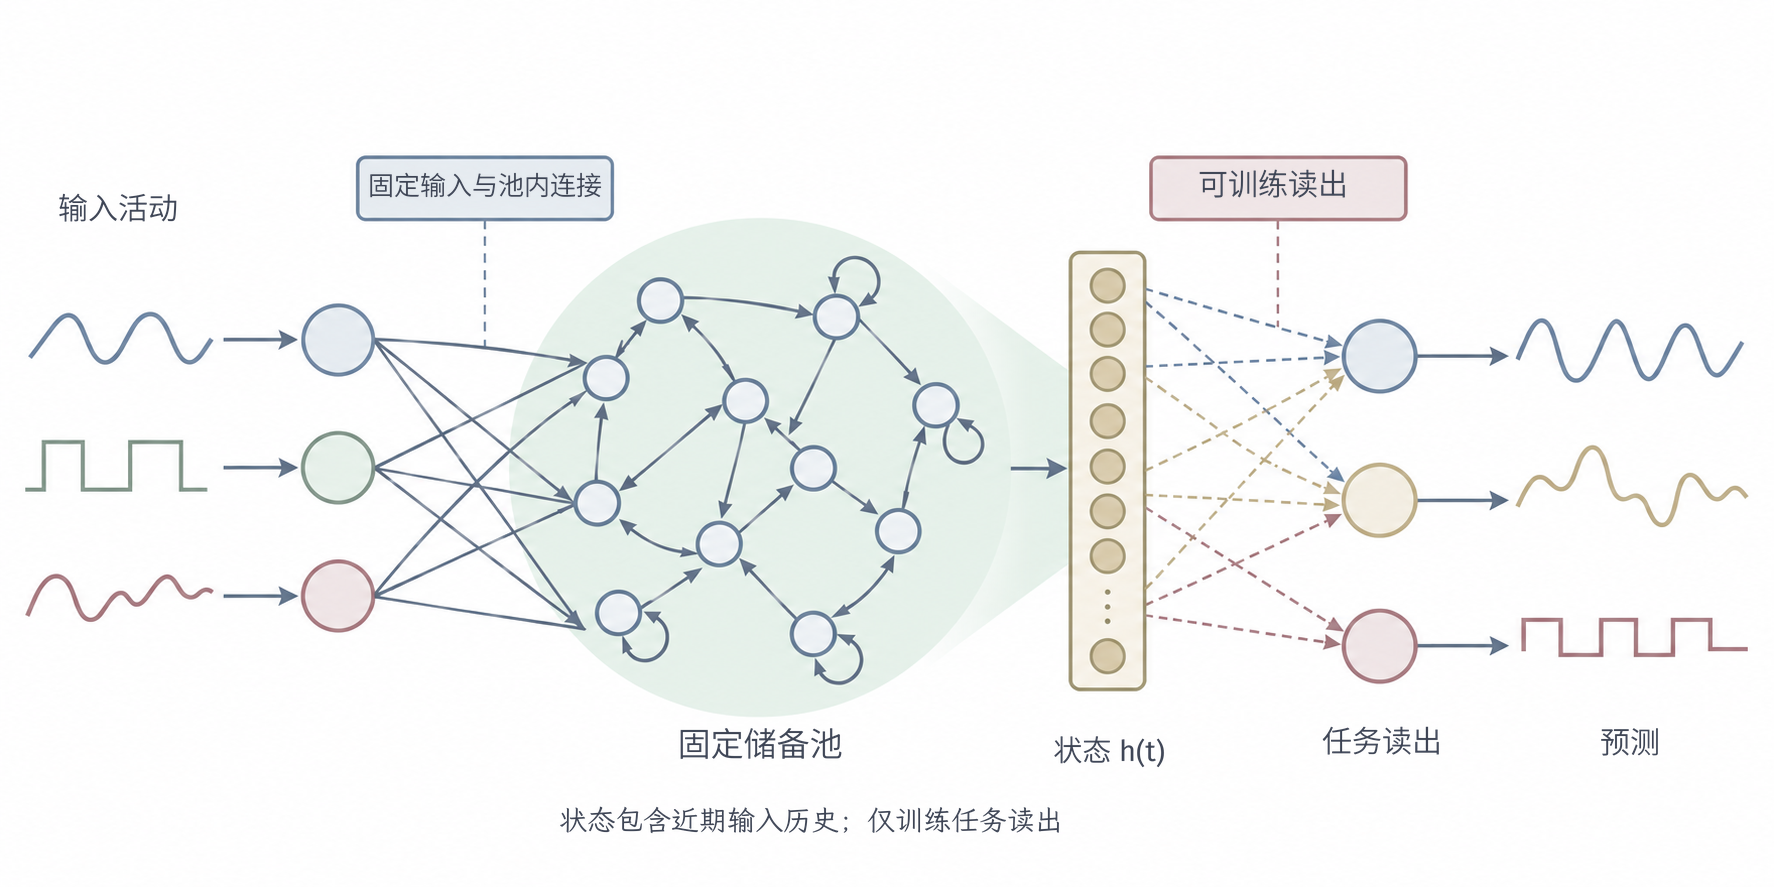
\includegraphics[width=150.199mm]{figures/05-neural-network-models/00-shared/generated/rnn-reservoir/figure.png}
  \caption{储备池计算的参数分工。输入进入固定的循环动态，多个内部单元共同形成随历史变化的状态，可训练读出将状态映射到目标。灰色连线表示固定连接，箭头表示参与拟合的读出；内部连接只示意结构，不表示某个随机生成样本。ESN使用连续值激活，LSM可由脉冲活动及其滤波响应形成读出特征。}
  \label{fig:rnn-reservoir}
\end{figure*}
\FloatBarrier

\subsection{ESN}
\label{sec:rnn-esn}

\term{回声状态网络}（echo state network, ESN）是一种以连续值循环状态提供历史特征的储备池模型，Jaeger的技术报告建立了其基本框架\scite{jaeger2001} 下面采用无输出反馈的泄漏积分版本，避免把真实目标或读出结果再送入储备池。令泄漏率$\alpha\in(0,1]$，更新为
\begin{equation}
  \begin{aligned}
    \widetilde{\bm{h}}^{(t)}&=\tanh\!\left(
      \bm{W}_{\mathrm{res}}\bm{h}^{(t-1)}
      +\bm{U}_{\mathrm{res}}\bm{x}_t+\bm{b}_{\mathrm{res}}\right),\\
    \bm{h}^{(t)}&=(1-\alpha)\bm{h}^{(t-1)}
       +\alpha\widetilde{\bm{h}}^{(t)}\text{。}
  \end{aligned}
  \label{eq:rnn-esn-update}
\end{equation}
$\bm{W}_{\mathrm{res}}\in\mathbb{R}^{m\times m}$、$\bm{U}_{\mathrm{res}}\in\mathbb{R}^{m\times d}$和偏置通常构造后固定。较小$\alpha$使每次状态变化较慢，但实际记忆还取决于循环矩阵、输入尺度和非线性响应。稀疏连接、输入缩放、泄漏率和状态维度均是可由验证选择的配置。

训练时先运行储备池，收集特征$\bm{z}_t=[1;\bm{x}_t;\bm{h}^{(t)}]\in\mathbb{R}^{1+d+m}$，分号表示向量拼接。初始若干步可能主要反映人为初态，常丢弃这段\term{洗出期}（washout），即先让系统接受输入、再开始拟合读出。洗出期剔除的是受初态影响的读出特征，任务标签所依赖的输入仍要进入状态更新；独立序列采用一致的洗出和重置规则。

对连续值目标，将$N$个有效状态按行堆成$\bm{Z}\in\mathbb{R}^{N\times(1+d+m)}$，相应目标堆成$\bm{Y}\in\mathbb{R}^{N\times q}$。线性读出参数为$\bm{R}\in\mathbb{R}^{(1+d+m)\times q}$，采用平方损失和岭惩罚时
\begin{equation}
  \begin{aligned}
    \bm{R}^{\star}&=\argmin_{\bm{R}}
      \lVert\bm{Z}\bm{R}-\bm{Y}\rVert_{\mathrm{F}}^2
      +\lambda\lVert\bm{R}\rVert_{\mathrm{F}}^2,\\
    \bm{R}^{\star}&=(\bm{Z}^{\top}\bm{Z}+\lambda\bm{I})^{-1}
      \bm{Z}^{\top}\bm{Y},\qquad \lambda>0\text{。}
  \end{aligned}
  \label{eq:rnn-esn-ridge}
\end{equation}
这里$\lVert\cdot\rVert_{\mathrm{F}}$是Frobenius范数。公式惩罚了包括截距在内的全部系数；若不惩罚截距，应改用相应对角惩罚矩阵并另查可逆性。实现时可解对应线性方程，公式中的逆矩阵表示其解。Softmax与交叉熵读出则产生另一种目标，按分类目标训练参数。

拟合出的$\bm{R}^{\star}$按列保存各输出坐标的权重。对列特征向量$\bm{z}_t$，连续值预测为$\widehat{\bm{y}}_t=(\bm{R}^{\star})^{\top}\bm{z}_t\in\mathbb{R}^{q}$；这与设计矩阵按行保存特征、$\bm{Z}\bm{R}^{\star}$逐行给出预测的约定一致。训练后将固定储备池的配置与拟合出的读出参数一同保存。处理新的独立序列时，按训练时约定的初始化、洗出和特征构造规则运行同一储备池，在有效读出位置用$\bm{R}^{\star}$形成预测；处理同一连续流时，则按约定延续状态。

任务读出希望状态主要由输入历史决定，初态差异随持续输入逐渐减弱。\term{回声状态性质}（echo state property, ESP）要求在约定的输入与状态范围内，相同持续输入驱动下，初始状态的影响最终消失。对式\eqref{eq:rnn-esn-update}，Tanh是1-Lipschitz，因而两个状态的距离满足
\begin{equation}
  \lVert\bm{h}^{(t)}-\bm{h}_{\mathrm{alt}}^{(t)}\rVert_2
    \leq\left(1-\alpha+\alpha\lVert\bm{W}_{\mathrm{res}}\rVert_2\right)
      \lVert\bm{h}^{(t-1)}-\bm{h}_{\mathrm{alt}}^{(t-1)}\rVert_2\text{。}
  \label{eq:rnn-esn-contraction}
\end{equation}
这里$\bm{h}^{(t)}$与$\bm{h}_{\mathrm{alt}}^{(t)}$表示初态不同、输入相同的两条轨迹。$\lVert\bm{W}_{\mathrm{res}}\rVert_2<1$给出统一收缩的充分条件，但不是必要条件。按谱半径缩放限制线性模式，非线性储备池还包含激活和输入驱动；相关反例与更精确条件见Yildiz等的分析\scite{yildiz2012}

初态影响消失也意味着一部分过去影响会衰减，适当的衰减使模型能适应新输入，过快衰减却可能丢掉任务证据。\term{记忆容量}（memory capacity）的一种线性测量方法，是对独立同分布的零均值标量输入，在方差有限且非零的条件下，分别学习各延迟的线性重构，再累加平方相关系数。若某个延迟的总体最小二乘重构量方差为零，通常的相关系数分母也为零；本文约定将该延迟的容量贡献按0计，表示这份线性重构没有恢复输入的变化。在状态为$m$维、读出仅使用状态且采用相应总体最小二乘定义的条件下，总线性记忆容量不超过$m$；这项容量指标衡量线性延迟重构，任务分类的准确率由相应目标另外评价\scite{jaeger2001memory} 读出优化利用已有特征，远期证据是否仍可区分则要从动态状态检验。

\subsection{LSM}
\label{sec:rnn-lsm}

输入也可能由带时间戳的事件构成，如传感器事件或神经脉冲。\term{液态状态机}（liquid state machine, LSM）用动态储备池的瞬时响应表示输入历史，代表性实现是固定的脉冲神经元回路，再学习状态读出。其名称强调利用持续变化的内部活动，不要求系统每次都收敛到一个稳定状态。

图~\ref{fig:rnn-lsm}把输入到任务输出的过程分开。输入是事件时，可以直接接入脉冲回路；连续观测则需按约定编码为输入脉冲。编码规则决定观测幅度、变化或时间如何转成回路接受的事件输入。
\begin{figure*}[htb]
  \centering
  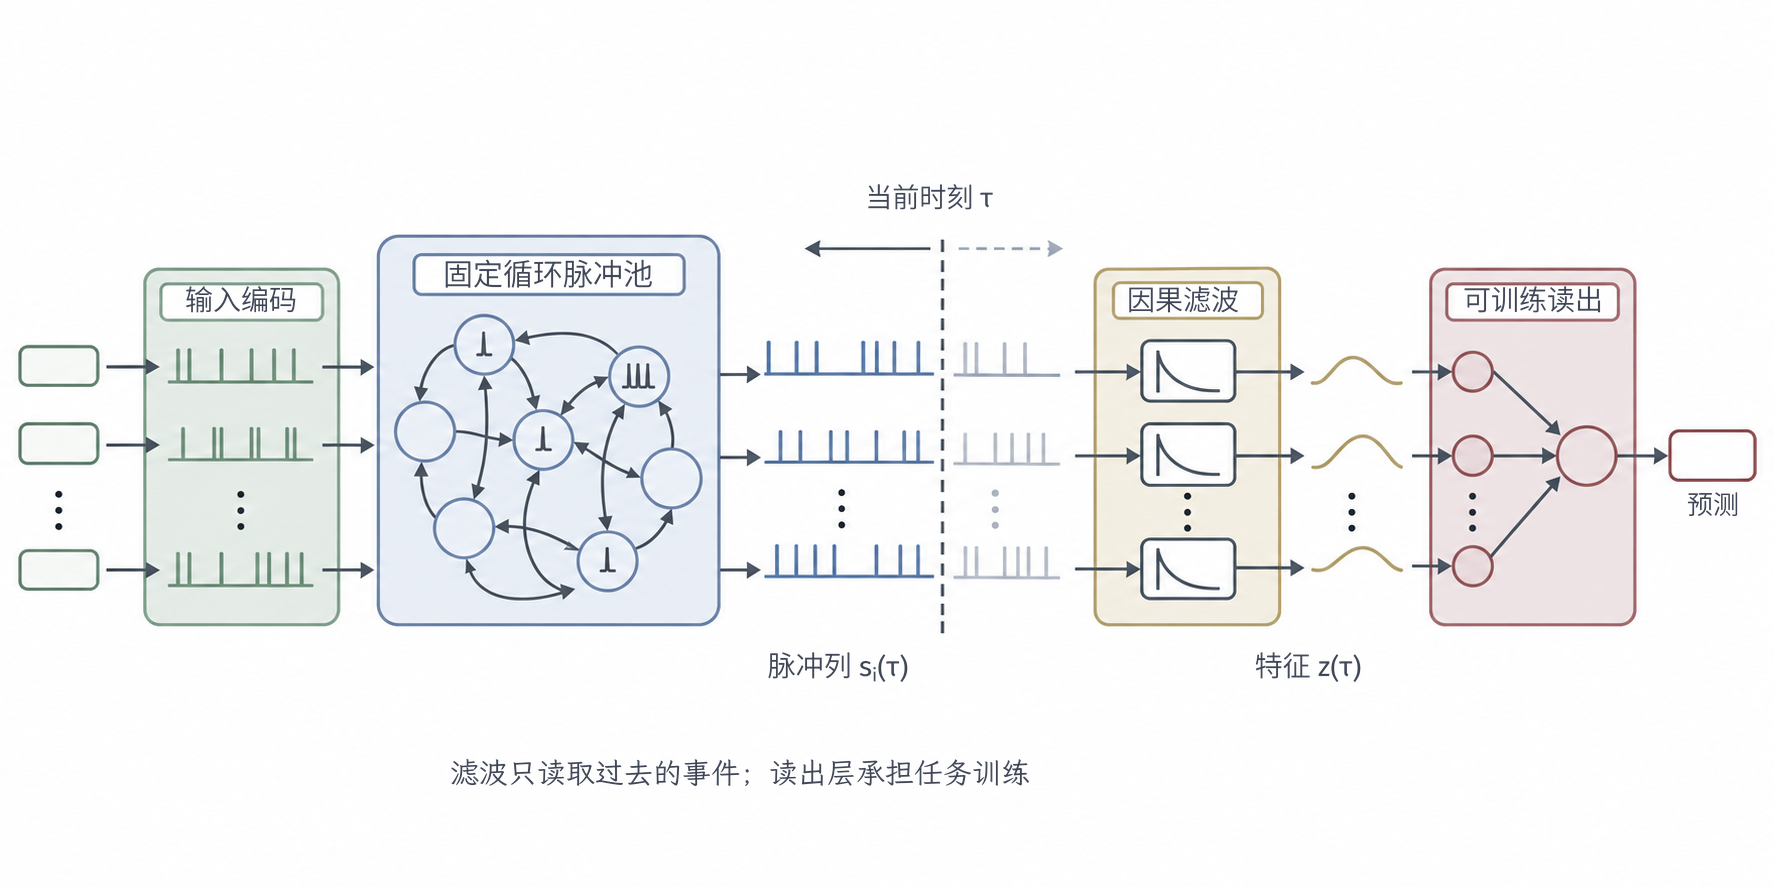
\includegraphics[width=150.199mm]{figures/05-neural-network-models/00-shared/generated/rnn-lsm/figure.png}
  \caption{LSM的输入、动态与读出。输入编码驱动固定的循环脉冲储备池，回路活动形成脉冲列$s_i(\tau)$；因果滤波将这些活动变成当前可读特征$\bm z(\tau)$，任务读出再映射为预测。反馈表示回路动态，滤波后的特征进入可训练任务读出。此处只训练任务读出，脉冲编码、回路参数与滤波核按约定固定。}
  \label{fig:rnn-lsm}
\end{figure*}
\FloatBarrier

回路中的状态比“这个时刻是否发出脉冲”更丰富。例如一个简化的漏积分发放单元可以写为
\begin{equation}
  \tau_{\mathrm m}\frac{\mathrm d v_i(\tau)}{\mathrm d\tau}
    =-(v_i(\tau)-v_{\mathrm{rest}})
      +I_i(\tau)+\sum_j w_{i,j}(\kappa_{\mathrm{syn}}*s_j)(\tau)\text{，}
  \label{eq:rnn-lsm-membrane}
\end{equation}
其中$v_i$是膜电位，$v_{\mathrm{rest}}$是静息电位，$\tau_{\mathrm m}>0$是泄漏时间常数，$I_i$表示换算到同一电位尺度的外部驱动，$w_{i,j}$是固定连接权重，$\kappa_{\mathrm{syn}}*s_j$是此前脉冲经过突触滤波后的作用。膜电位达到阈值时发出脉冲并重置；这里省略不应期等细节。持续的膜电位、突触响应和反馈活动共同承载输入历史，当前输入停止后，内部影响仍可能延续\scite{maass2002}

若第$i$个单元在时刻$\tau_{i,k}$发出脉冲，其脉冲列为$s_i(\tau)=\sum_k\delta(\tau-\tau_{i,k})$，$\delta$是Dirac脉冲。它不是某一时刻的普通有限函数值，而是用积分记录一次单位事件：与连续权重函数相乘后积分，就取出该函数在发放时刻的值。因而可以用因果滤波核$\kappa_i$形成特征：
\begin{equation}
  z_i(\tau)=\int_{-\infty}^{\tau}\kappa_i(\tau-u)s_i(u)\,\mathrm du,
  \qquad \kappa_i(v)=e^{-v/\tau_i}\mathbf 1_{\{v\geq0\}}\text{。}
  \label{eq:rnn-lsm-filter}
\end{equation}
$\tau_i>0$是特征衰减时间常数，$\mathbf 1$是指示函数。采用事件发生后立即计入当前状态的约定，积分可以逐个发放时刻展开为
\begin{equation}
  z_i(\tau)=\sum_{k:\,\tau_{i,k}\leq\tau}
    \exp\!\left(-\frac{\tau-\tau_{i,k}}{\tau_i}\right)\text{。}
  \label{eq:rnn-lsm-event-sum}
\end{equation}
每次脉冲向$z_i$加入$1$，此后按已经过去的时间衰减；未来事件不参与求和。脉冲编码的进一步说明见第~\ref{sec:snn-coding}节。这一步是状态读取：把回路活动整理成有限维、可供后续计算的$\bm z(\tau)$。这些滤波特征保留了所选脉冲响应，膜电位和其他突触变量仍可能未被记录；读出获得的信息范围由所选特征决定。

读出是从这些状态特征到任务预测的映射，作用相当于前馈网络的输出头。读取特征与产生任务答案是两步计算；一个常用读出为
\begin{equation}
  \bm a(\tau)=\bm V\bm z(\tau)+\bm b,
  \qquad\widehat{\bm y}(\tau)=g(\bm a(\tau))\text{，}
  \label{eq:rnn-lsm-readout}
\end{equation}
其中$\bm z\in\mathbb R^m$、$\bm V\in\mathbb R^{q\times m}$。回归可取$g$为恒等映射，分类可取Sigmoid或Softmax；训练样本提供目标，监督$\bm V,\bm b$的学习。读出也可以是更复杂的可训练网络，两种历史若产生相同的$\bm z$，只读取$\bm z$的确定性读出就给出相同结果，因而特征本身也要保留任务所需区别。

\begin{example}[从脉冲活动到预测]
  \label{ex:rnn-lsm-readout}
  假设两个单元均使用时间常数2：第一个在时刻1和3发放，第二个只在时刻2发放。在时刻4，特征为$z_1=e^{-3/2}+e^{-1/2}\approx0.830$、$z_2=e^{-1}\approx0.368$。若教学例子中的回归读出为$\widehat y=2z_1-z_2-0.5$，便得到约$0.791$。脉冲与滤波决定特征，系数$(2,-1)$和偏置决定这些特征怎样形成任务答案；训练用状态特征及对应目标估计读出系数和偏置。
\end{example}

训练时先按实际顺序驱动回路，在约定时刻收集状态特征及对应目标，再拟合读出。平方损失的线性读出可沿用ESN的岭回归，分类读出则使用相应分类目标。独立事件序列需要重置或约定初态，同一连续流可以延续状态；采集特征时仍须遵守预测时的信息范围。

LSM对长期依赖的帮助来自动态特征的时间范围：较慢的突触／滤波响应保留较久的影响，循环反馈还可延长或重组这种影响。过快的衰减会丢掉远期证据，过强反馈可能使无关活动持续，多个历史也可能被压成相同特征。固定回路减少了训练循环参数的困难，但读出能否利用长期历史，取决于特征是否仍可区分任务所需的历史。

ESN主要以连续值激活表示状态，LSM利用脉冲时刻及其动态响应。事件稀疏时可采用事件驱动计算，数字仿真的更新、通信和读出成本仍需计入。脉冲编码、膜电位模型与可塑性学习在后续脉冲神经网络章展开，这里的动态负责提供历史表示，监督训练负责把这些表示转换成任务预测。

\FloatBarrier
\section{基于控制门的循环神经网络}
\label{sec:rnn-gated}

储备池把动态固定下来、绕开了训练难题，但固定动态无法\emph{针对具体任务}决定哪些信息该记、哪些该忘；普通RNN虽然可训练，却把旧状态和新输入混合后用同一个Tanh整体变换，无法对个别内容单独保留或清除。门控网络给出第三条路：让网络自己学会一些由输入和状态计算的\emph{开关系数}，逐坐标地控制信息的保留、写入和读出。\term{控制门}（gate）就是这样一组系数，用逐元素乘法作用在信息流上；Sigmoid把每个系数压到$(0,1)$之间，可以理解为“这扇门开多大、让信息通过多少”，而且门是连续可微的，能够随训练逐步调整。门的参数和其他参数一样，由最终任务损失更新——因此“该在什么时候记住什么”不是人工规则，而是从任务中学来的。本节先介绍机制更完整的LSTM，再介绍更精简的GRU。

\subsection{LSTM}
\label{sec:rnn-lstm}

\term{长短期记忆}（long short-term memory, LSTM）针对普通RNN“所有记忆都挤在同一个被反复非线性变换的状态里”的问题，做了一个关键拆分：把\emph{长期保存的记忆}$\bm{c}^{(t)}$和\emph{当前对外输出的隐藏表示}$\bm{h}^{(t)}$分成两条独立的通路。记忆通路允许信息近乎不变地长期留存（等需要时再取用），隐藏表示则服务于当前一步的输出。原始LSTM发表于1997年，常用的遗忘门是后来加入的；以下讲解带遗忘门、无窥孔连接的常用版本\scite{hochreiter1997}

为什么这个拆分能缓解梯度消失？核心在于记忆通路采用\emph{加法}更新（旧记忆加上新内容），而不是像普通RNN那样每一步都整体乘一个非线性矩阵。这为信息保留提供了一条“走廊”：只要门选择让旧记忆原样通过，很久以前写下的内容就能沿走廊几乎无衰减地走到很远的输出。先看各门如何计算。令$\bm{c}^{(t)}\in\mathbb{R}^{m}$是记忆状态，$\bm{h}^{(t)}\in\mathbb{R}^{m}$是隐藏输出。门均读取$[\bm{x}_t;\bm{h}^{(t-1)}]\in\mathbb{R}^{d+m}$，计算
\begin{equation}
  \begin{aligned}
    \bm{i}^{(t)}&=\operatorname{sigmoid}\!\left(
      \bm{A}_{\mathrm{i}}[\bm{x}_t;\bm{h}^{(t-1)}]+\bm{b}_{\mathrm{i}}\right),\\
    \bm{f}^{(t)}&=\operatorname{sigmoid}\!\left(
      \bm{A}_{\mathrm{f}}[\bm{x}_t;\bm{h}^{(t-1)}]+\bm{b}_{\mathrm{f}}\right),\\
    \bm{o}^{(t)}&=\operatorname{sigmoid}\!\left(
      \bm{A}_{\mathrm{o}}[\bm{x}_t;\bm{h}^{(t-1)}]+\bm{b}_{\mathrm{o}}\right),\\
    \widetilde{\bm{c}}^{(t)}&=\tanh\!\left(
      \bm{A}_{\mathrm{c}}[\bm{x}_t;\bm{h}^{(t-1)}]+\bm{b}_{\mathrm{c}}\right)\text{。}
  \end{aligned}
  \label{eq:rnn-lstm-gates}
\end{equation}
每个$\bm{A}$属于$\mathbb{R}^{m\times(d+m)}$，每个偏置属于$\mathbb{R}^{m}$。输入门$\bm{i}^{(t)}$决定候选记忆写入多少，遗忘门$\bm{f}^{(t)}$决定旧记忆保留多少，输出门$\bm{o}^{(t)}$决定记忆的变换结果读出多少：
\begin{equation}
  \begin{aligned}
    \bm{c}^{(t)}&=\bm{f}^{(t)}\odot\bm{c}^{(t-1)}
       +\bm{i}^{(t)}\odot\widetilde{\bm{c}}^{(t)},\\
    \bm{h}^{(t)}&=\bm{o}^{(t)}\odot\tanh\!\left(\bm{c}^{(t)}\right)\text{。}
  \end{aligned}
  \label{eq:rnn-lstm-update}
\end{equation}
遗忘门值接近1时保留旧记忆，接近0时清除相应坐标。新旧信息在记忆路径上相加，隐藏输出则经过Tanh和输出门，记忆状态可以保留当前未必需要输出的信息。遗忘门使持续运行的网络能够清除不再相关的旧内容\scite{gers2000}

图~\ref{fig:rnn-lstm-cell}把各门的作用放在同一计算图中。三个Sigmoid模块输出门值，控制“通过多少”；与它们并排的Tanh模块产生候选记忆$\widetilde{\bm c}^{(t)}$，提供“写入什么”，数值可以为正或负。门与候选都取决于当前输入和此前状态，因此同一单元可以在不同输入位置采用不同的保留和写入策略。

\begin{figure*}[htb]
  \centering
  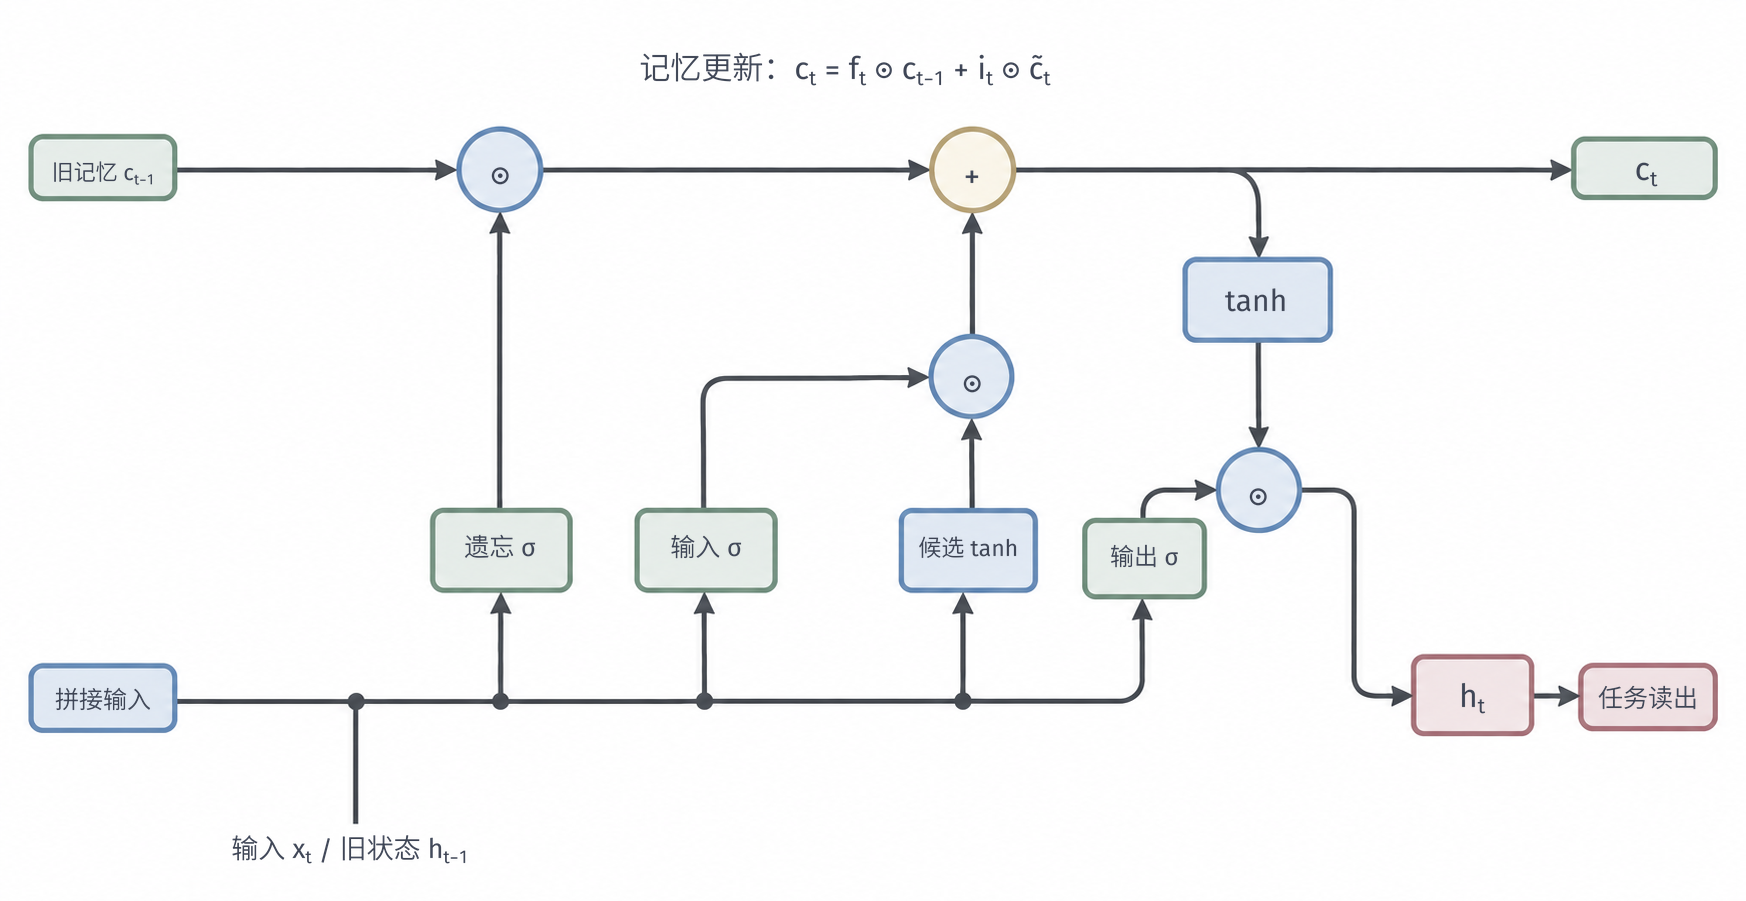
\includegraphics[width=147.828mm]{figures/05-neural-network-models/00-shared/generated/rnn-lstm-cell/figure.png}
  \caption{LSTM更新与任务读出。框外左侧为当前输入$\bm x_t$和旧状态$\bm h^{(t-1)},\bm c^{(t-1)}$，右侧为新状态和预测$\widehat{\bm y}_t=g(\bm V\bm h^{(t)}+\bm c)$。三个Sigmoid模块分别产生遗忘门、输入门和输出门，Tanh框产生候选记忆；圆形$\odot$与$+$分别表示逐元素乘法和相加。门值0阻断对应路径的信息，门值1让信息通过。}
  \label{fig:rnn-lstm-cell}
\end{figure*}
\FloatBarrier

如果暂把门与候选值看作已给定量，记忆路径对旧记忆的直接导数为$\operatorname{diag}(\bm{f}^{(t)})$。沿这条路径从$s$到$t$有
\begin{equation}
  \left.\frac{\partial\bm c^{(t)}}{\partial\bm c^{(s)}}\right|_{\mathrm{direct}}
    =\operatorname{diag}\!\left(\prod_{u=s+1}^{t}\bm f^{(u)}\right)\text{，}
  \label{eq:rnn-lstm-direct-memory}
\end{equation}
乘积按坐标进行。与普通RNN的$\bm D\bm W$相比，这条路径用可学习的保留率替代反复稠密混合；需要保存的坐标可令遗忘门接近1，并用较小输入门减少覆盖。这改变了式\eqref{eq:rnn-path-length-rate}中的逐步增益，通常没有缩短传播步数。但完整状态的Jacobian矩阵还包含$\bm h^{(t-1)}$影响各门和候选记忆的其他路径，直接路径与这些间接路径共同构成总导数。

\begin{example}[门值决定保留和写入]
  \label{ex:rnn-lstm-retention}
  考察一个记忆坐标，假设旧值为$2$，本步遗忘门为$0.9$、输入门为$0.2$、候选值为$0.5$。沿图~\ref{fig:rnn-lstm-cell}读取，左上$\odot$保留$0.9\times2=1.8$，中间$\odot$写入$0.2\times0.5=0.1$，再由上方$+$得到新记忆$1.9$。若输出门为$0.5$，右侧$\odot$产生隐藏输出$0.5\tanh(1.9)\approx0.478$，而非直接输出记忆值$1.9$。

  若之后100步不写入且遗忘门都为$0.99$，这份记忆沿直接路径的保留比例为$0.99^{100}\approx0.366$；门值为$0.9$时仅约$2.66\times10^{-5}$。加性记忆提供了可选择的保留率；小于1的门沿直接路径连续相乘，仍产生与距离有关的衰减。
\end{example}

图~\ref{fig:rnn-lstm-numerical-step}把例~\ref{ex:rnn-lstm-retention}扩展到两个记忆坐标。第一通道取较大的遗忘门和较小的输入门，主要保留旧值；第二通道反过来，主要写入候选值。$\odot$只在相同坐标之间相乘，不会把第一通道的门值作用到第二通道。两个通道可以采用不同的保留和写入比例。
\begin{figure*}[htbp]
  \centering
  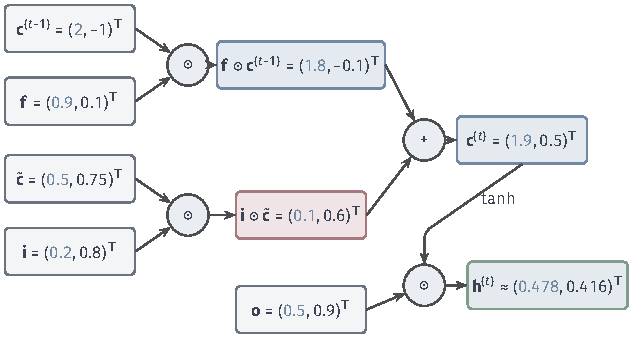
\includegraphics[width=107.107mm]{figures/05-neural-network-models/00-shared/tikz/rnn-lstm-numerical-step/figure.pdf}
  \caption{二维LSTM的一步数值走查。蓝色与深灰数字分别表示两个通道；保留分支计算$\bm f\odot\bm c^{(t-1)}$，写入分支计算$\bm i\odot\widetilde{\bm c}$，二者相加得到新记忆，再经$\bm o\odot\tanh(\bm c^{(t)})$得到隐藏状态。所有数值均由图内向量逐坐标计算，第二通道结果为$0.9\tanh(0.5)\approx0.416$。图中暂把门值和候选值视为已知，不展开它们的仿射计算。}
  \label{fig:rnn-lstm-numerical-step}
\end{figure*}
\FloatBarrier

记忆保持与信息读出仍要同时满足。即使直接路径没有明显衰减，过多写入也会覆盖证据；输出门较小或$\tanh(\bm c)$饱和时，任务损失仍可能难以作用于这段记忆。LSTM提供按任务选择保留、写入和读出的机制，完整梯度与预测表现需要对整个状态和读出分析。

训练仍使用BPTT，只需对记忆和隐藏两组状态共同求导。仅计上述单元，参数量为$4m(d+m+1)$，每步稠密仿射计算为$O(m(d+m))$，常数来自四组变换。增大初始遗忘门偏置可使初始保留比例较高，但门饱和也会减小自身的导数；这一选择需与长度和输入尺度匹配。

变体通常改变某条信息通路。\term{窥孔连接}（peephole connections）让门额外读取记忆坐标；耦合输入门与遗忘门可令$\bm{i}^{(t)}=\bm{1}-\bm{f}^{(t)}$，减少一组自由门。这些变体改变了门的依赖或自由度，适合程度需要在具体任务上比较\scite{greff2017}

% 避免两条完整变体引文在页底连续堆叠。
\Needspace{10\baselineskip}
若希望保留较宽记忆而减少循环映射成本，投影LSTM把记忆输出映射到更小的循环隐藏空间，使记忆宽度和循环宽度分开。投影把循环映射改为较小宽度，参数计数与前述等宽单元相应不同\scite{sak2014projection}

\subsection{GRU}
\label{sec:rnn-gru}

若希望简化状态管理，可以把记忆与隐藏输出合为一组变量。\term{门控循环单元}（gated recurrent unit, GRU）用更新门决定旧状态与候选状态的混合比例，用重置门控制候选计算怎样读取旧状态。这里采用Cho等原始形式的记号：更新门值越大，旧状态保留越多\scite{cho2014}

对同宽状态，方程为
\begin{equation}
  \begin{aligned}
    \bm{z}^{(t)}&=\operatorname{sigmoid}\!\left(
      \bm{U}_{\mathrm{z}}\bm{x}_t+\bm{W}_{\mathrm{z}}\bm{h}^{(t-1)}
      +\bm{b}_{\mathrm{z}}\right),\\
    \bm{r}^{(t)}&=\operatorname{sigmoid}\!\left(
      \bm{U}_{\mathrm{r}}\bm{x}_t+\bm{W}_{\mathrm{r}}\bm{h}^{(t-1)}
      +\bm{b}_{\mathrm{r}}\right),\\
    \widetilde{\bm{h}}^{(t)}&=\tanh\!\left(
      \bm{U}_{\mathrm{h}}\bm{x}_t
      +\bm{W}_{\mathrm{h}}(\bm{r}^{(t)}\odot\bm{h}^{(t-1)})
      +\bm{b}_{\mathrm{h}}\right),\\
    \bm{h}^{(t)}&=\bm{z}^{(t)}\odot\bm{h}^{(t-1)}
      +(\bm{1}-\bm{z}^{(t)})\odot\widetilde{\bm{h}}^{(t)}\text{。}
  \end{aligned}
  \label{eq:rnn-gru-update}
\end{equation}
每组$\bm{U}$、$\bm{W}$和偏置的形状与普通RNN相同。重置门接近零时，候选计算弱化旧状态；更新门接近1时，即使候选发生变化，输出也主要保留旧值。重置门调节候选读入的旧状态，更新门调节候选写入的比例，两者作用于不同计算位置。

图~\ref{fig:rnn-gru-cell}显示了候选分支和保留分支。单独看保留分支，其直接传播系数为$\bm{z}^{(t)}$；完整导数还包含门和候选的变化，与LSTM一样，直接分支之外的依赖也参与求导。

\begin{figure*}[htb]
  \centering
  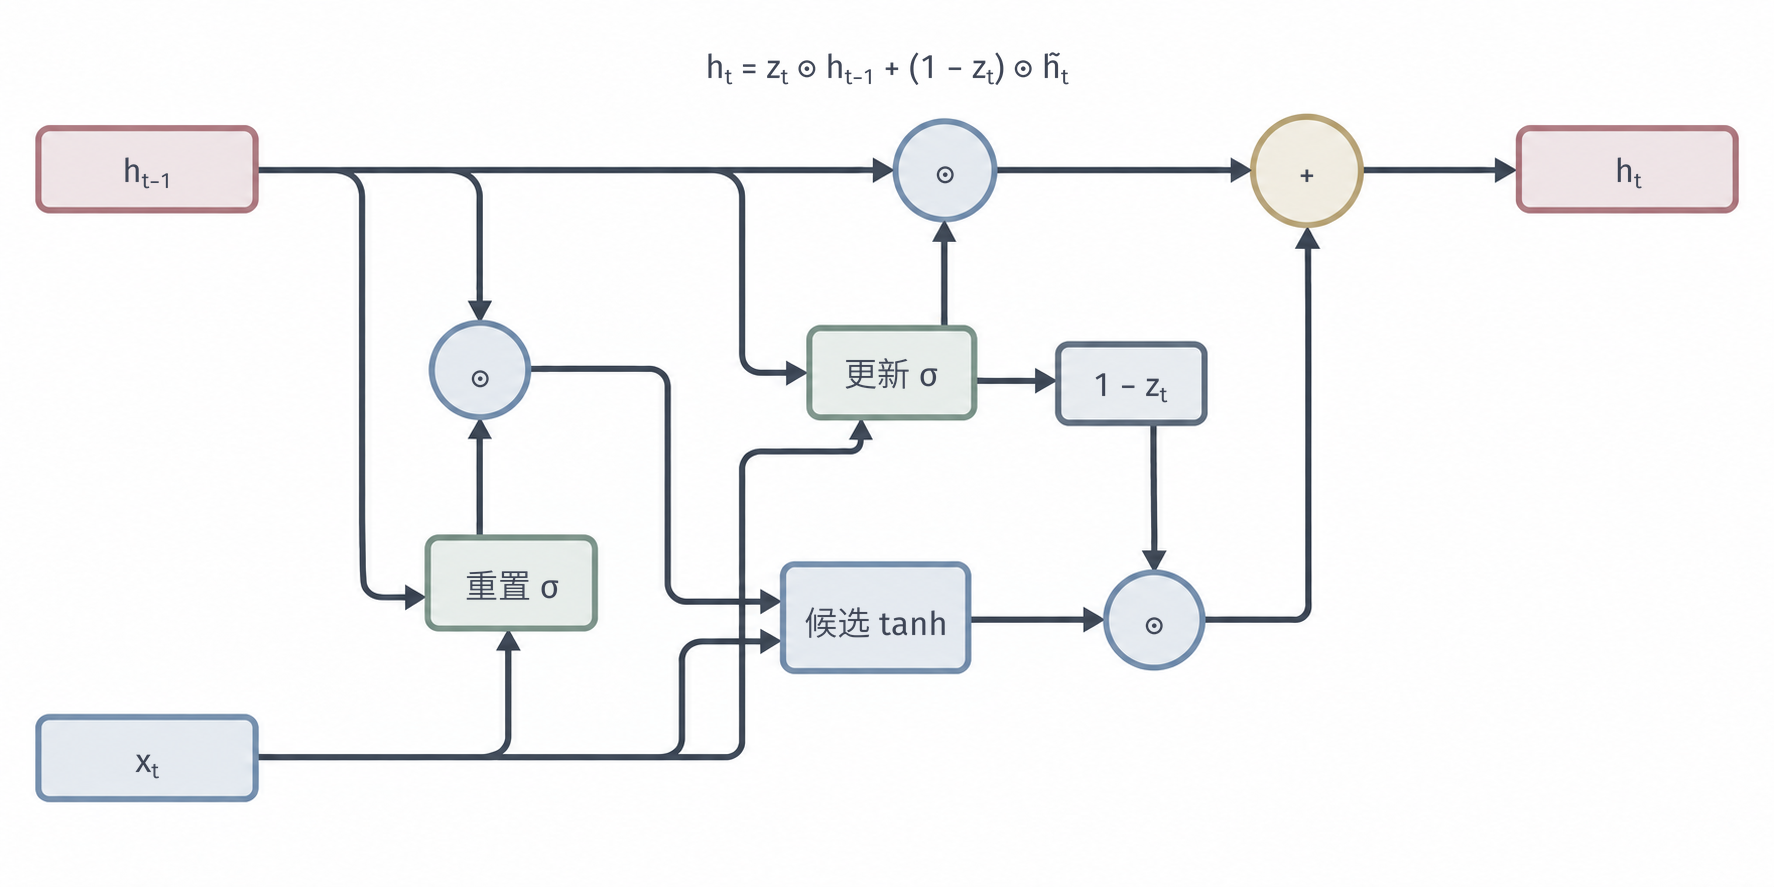
\includegraphics[width=150.199mm]{figures/05-neural-network-models/00-shared/generated/rnn-gru-cell/figure.png}
  \caption{GRU的状态更新。左侧输入为$\bm x_t$和旧状态$\bm h^{(t-1)}$，右侧输出为新状态。组合输入将当前输入与旧状态一并送入门和候选模块。重置门参与候选计算；顶部两个$\odot$框则显式形成$\bm z^{(t)}\odot\bm h^{(t-1)}$与$(\bm1-\bm z^{(t)})\odot\widetilde{\bm h}^{(t)}$，再相加得到新状态。任务预测还需在新状态之后另接读出。}
  \label{fig:rnn-gru-cell}
\end{figure*}
\FloatBarrier

GRU的长期保留对应更新门调节的直达分支。在需要延续记忆的坐标上，$\bm z^{(t)}$接近1时，状态更新接近复制旧值，沿保留路径的系数为各步$\bm z$的逐坐标乘积。候选分支的权重$\bm1-\bm z$同时较小，减少无关新输入覆盖已有状态。更新门接近0时则更多采用候选，允许网络改变当前记忆内容。

重置门的作用发生在候选计算中：它调节形成新候选时读取的旧状态量。重置门接近0、更新门接近1时，网络仍可以保留旧状态；更新门接近0时，即使重置门较大，旧信息也要通过非线性候选重新表达。没有独立记忆状态与输出门，还使GRU的保留内容和当前对外表示耦合得更紧。门接近恒等复制能改善一条梯度路径，门饱和、候选混合及读出仍可能限制长期学习。

在只用一组偏置的上述形式中，GRU单元参数量为$3m(d+m+1)$，少于等宽LSTM的四组变换，也只维护一个$m$维状态。代价是没有独立的记忆状态和输出门，存储与对外表示更直接地耦合。三组变换减少了等宽时的参数和状态存储，任务效果还取决于这种状态耦合是否适合目标；比较可在相近预算与预测条件下进行。

文献与软件还存在不同约定：有的把更新门定义为新候选的写入比例，有的把重置门放在$\bm{W}_{\mathrm{h}}\bm{h}^{(t-1)}$之后。前一种可通过交换$\bm{z}$与$1-\bm{z}$对应，后一种一般不能交换矩阵乘法与逐元素乘法，因此并非完全相同的更新。方程、偏置组数和门顺序共同确定具体GRU的计算与参数计数。

\FloatBarrier
\section{基于注意力的循环神经网络}
\label{sec:rnn-attention}

门控让网络\emph{更好地保存}信息，但前面的编码器—解码器结构还有一个结构性瓶颈：在式\eqref{eq:rnn-encoder-decoder}中，无论源序列多长，解码器都只能从编码器的\emph{同一个末状态}$\bm c_{\mathrm{enc}}=\bm h^{(T)}$读取信息。这等于要求网络把一整句话的所有细节压缩进一个固定维度的向量；输入越长，需要同时保存并区分的细节越多，这个瓶颈就越拥挤——即使编码器用的是LSTM也难以避免。

一个自然的想法是：\emph{不要只留摘要，把编码器每个位置的状态都保留下来，让解码器在生成每个词时“回头看”、按需取用}。翻译到当前词需要源句中的某个短语时，就给那个位置较高的权重；生成下一个词时再重新分配。这种根据当前需要动态加权读取一组表示的机制，就是\term{注意力机制}（attention mechanism）。它改变的是历史的\emph{读取方式}（而非保存方式），与门控（改变保存方式）正交，二者常一起使用。

\subsection{注意力机制}
\label{sec:rnn-attention-mechanism}

\term{注意力机制}（attention mechanism）根据当前计算需求给一组表示分配权重，再加权聚合：解码器需要的信息改变时，读取的上下文也随之改变。令编码器状态为$\bm{h}_1,\ldots,\bm{h}_T\in\mathbb{R}^{m}$，这里下标表示被保存的位置，$\bm{h}_t=\bm{h}^{(t)}$。对第$j$个解码步，给定查询$\bm{q}^{(j)}\in\mathbb{R}^{r}$，该向量承载本步解码需要读取哪些信息的线索，可以由解码状态或其变换产生。后面两种架构将确定查询采用旧状态还是本步新状态；此处先把查询视为已知，计算
\begin{equation}
  \begin{aligned}
    e_{j,t}&=a(\bm{q}^{(j)},\bm{h}_t),\\
    \alpha_{j,t}&=\frac{\exp(e_{j,t})}
       {\sum_{u=1}^{T}\exp(e_{j,u})},\\
    \bm{c}^{(j)}&=\sum_{t=1}^{T}\alpha_{j,t}\bm{h}_t\text{。}
  \end{aligned}
  \label{eq:rnn-attention}
\end{equation}
评分函数$a$比较查询与候选表示的相关程度。Softmax使权重非负且总和为1，$\bm{c}^{(j)}$是本步的动态上下文。归一化只在有效输入位置上进行，填充位置通过掩码排除。对很大的得分减去最大值再取指数，不改变权重，却可避免指数溢出。

评分可以通过非线性组合学习，也可以使用内积。\term{加性注意力}（additive attention）先把查询和编码状态投影到同一评分空间，再给出标量：
\begin{equation}
  e_{j,t}=\bm{v}_{\mathrm{a}}^{\top}\tanh\!\left(
     \bm{W}_{\mathrm{q}}\bm{q}^{(j)}
     +\bm{W}_{\mathrm{h}}\bm{h}_t+\bm{b}_{\mathrm{a}}\right)\text{。}
  \label{eq:rnn-additive-attention}
\end{equation}
设评分空间宽度为$a$，则$\bm{W}_{\mathrm{q}}\in\mathbb{R}^{a\times r}$、$\bm{W}_{\mathrm{h}}\in\mathbb{R}^{a\times m}$、$\bm{v}_{\mathrm{a}},\bm{b}_{\mathrm{a}}\in\mathbb{R}^{a}$。它允许查询和编码状态原本具有不同维度。

\term{点积注意力}（dot-product attention）直接用内积评分，在$r=m$时可取$e_{j,t}=\langle\bm{q}^{(j)},\bm{h}_t\rangle$；一般形式可取$e_{j,t}=(\bm{q}^{(j)})^{\top}\bm{W}_{\mathrm{a}}\bm{h}_t$，其中$\bm{W}_{\mathrm{a}}\in\mathbb{R}^{r\times m}$。点积形式便于批量矩阵计算，加性形式通过额外非线性改变评分函数，两者的适合程度仍由任务和宽度决定。Transformer章会继续讨论缩放、多头和位置编码，这里只需理解评分、归一化和聚合。

\begin{example}[权重与上下文]
  \label{ex:rnn-attention-context}
  假设本步对三个位置的得分为$0,\log2,0$，相应状态为$(1,0)^{\top}$、$(0,2)^{\top}$、$(1,1)^{\top}$。归一化权重为$(1/4,1/2,1/4)$，上下文为$(1/2,5/4)^{\top}$。第二个位置贡献较大，但上下文仍混合了三个状态；软聚合把多个状态的贡献相加，最终预测还取决于这些状态的内容及后续计算。
\end{example}

\subsection{网络结构}
\label{sec:rnn-attentive-architecture}

动态上下文可以参与解码状态更新，也可以在更新后参与输出。Bahdanau等的模型用此前解码状态查询编码表示，先形成$\bm{c}^{(j)}$，再计算本步状态：
\begin{equation}
  \begin{aligned}
    \bm{q}^{(j)}&=\bm{s}^{(j-1)},\\
    \bm{s}^{(j)}&=F_{\mathrm{dec}}\!\left(
      \bm{s}^{(j-1)},\bm{e}(y_{j-1}),\bm{c}^{(j)}\right),\\
    \bm{p}^{(j)}&=G\!\left(\bm{s}^{(j)},\bm{c}^{(j)},\bm{e}(y_{j-1})\right)\text{。}
  \end{aligned}
  \label{eq:rnn-bahdanau-order}
\end{equation}
$G$是输出概率映射，包含所需的可学习变换和归一化。编码器可以双向读取输入，使每个位置的表示同时包含前后上下文；编码器读取完整源输入，解码器生成时仍只使用此前目标\scite{bahdanau2015}

Luong等则先计算本步解码状态，再用该状态查询，形成融合后的输出表示：
\begin{equation}
  \begin{aligned}
    \bm{s}^{(j)}&=F_{\mathrm{dec}}\!\left(
      \bm{s}^{(j-1)},\bm{e}(y_{j-1})\right),\\
    \bm{q}^{(j)}&=\bm{s}^{(j)},\qquad
    \widetilde{\bm{s}}^{(j)}=
       \tanh\!\left(\bm{W}_{\mathrm{c}}[\bm{s}^{(j)};\bm{c}^{(j)}]\right),\\
    \bm{p}^{(j)}&=\operatorname{softmax}\!\left(
      \bm{V}_{\mathrm{a}}\widetilde{\bm{s}}^{(j)}+\bm{b}_{\mathrm{a}}\right)\text{。}
  \end{aligned}
  \label{eq:rnn-luong-order}
\end{equation}
其输入馈送变体还把前一步融合表示送入下一步解码。两个模型的关键区别之一是查询产生的时机和上下文进入的路径，若把当前状态查询放进式\eqref{eq:rnn-bahdanau-order}而保留其余依赖，查询与本步更新就互相等待；具体架构通过明确先后次序建立可执行的计算\scite{luong2015}

\term{全局注意力}（global attention）对全部有效输入位置评分，生成$S$个符号通常需要$ST$个位置对评分。\term{局部注意力}（local attention）只考虑某个位置附近的窗口，可固定窗口推进方式，也可由状态预测中心。窗口降低了读取范围与评分数量，但可能遗漏远处证据；可学习中心、连续位置权重和边界处理还需明确。局部方法预先限制本步评分的候选位置；全局权重集中则仍在完整位置集合上评分。

图~\ref{fig:rnn-attention-paths}采用先查询、后更新的组织方式。保存的编码状态建立了一条从输出直接读取早期位置的路径，减轻了所有细节只能经过编码末状态的限制。它同时需要保存整段编码表示，每个生成步还要执行读取，代价与固定状态读出不同。

\begin{figure*}[htb]
  \centering
  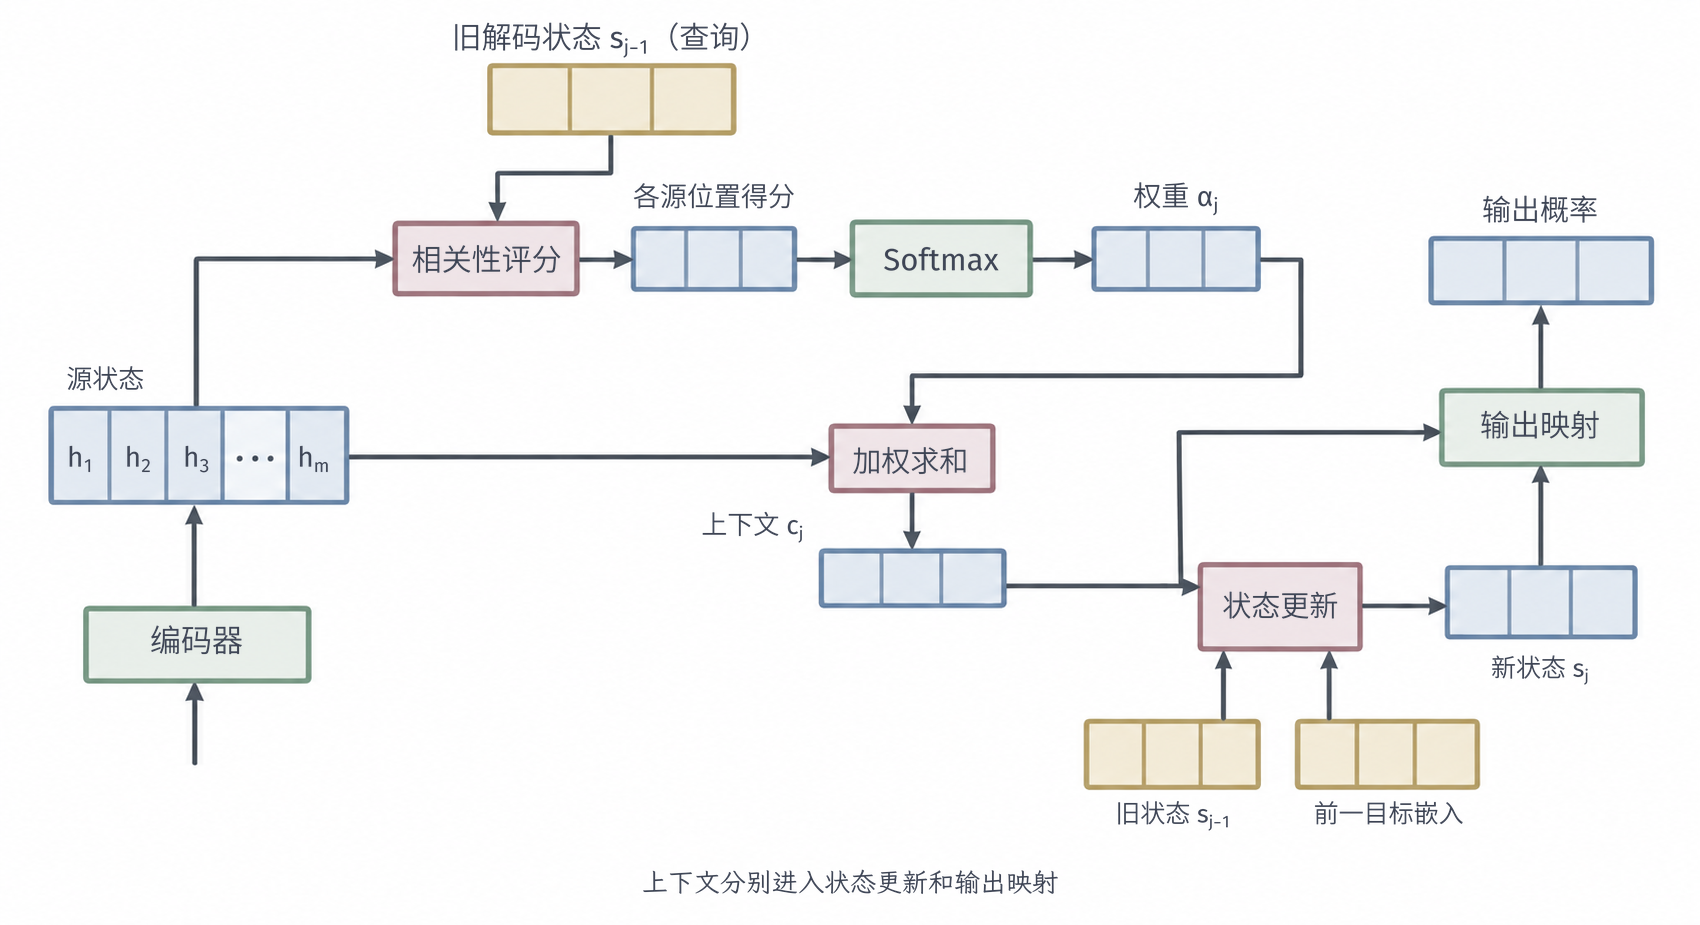
\includegraphics[width=143.933mm]{figures/05-neural-network-models/00-shared/generated/rnn-attention-paths/figure.png}
  \caption{带注意力的一个解码步。左侧为保存的编码状态$\bm h_{1:T}$、旧解码状态和此前目标的嵌入，右侧为新解码状态和输出概率。查询先用旧解码状态产生权重$\bm\alpha_j=(\alpha_{j,1},\ldots,\alpha_{j,T})$，上下文再进入更新与输出映射；输出映射还可读取目标嵌入。编码状态在各解码步重复读取，图中不重新执行编码器。}
  \label{fig:rnn-attention-paths}
\end{figure*}
\FloatBarrier


注意力对长期依赖的作用，可以从读取路径直接看出。暂固定本步评分和权重时，动态上下文对第$t$个编码状态的直接导数为
\begin{equation}
  \left.\frac{\partial\bm c^{(j)}}{\partial\bm h_t}\right|_{\bm\alpha_j\ \mathrm{fixed}}
       =\alpha_{j,t}\bm I\text{。}
  \label{eq:rnn-attention-direct-path}
\end{equation}
该分支从上下文直接到保存的表示，不再要求第$t$个状态经过其后全部编码状态才能被读取。权重若均匀，系数为$1/T$；若本步评分集中于相关位置，相应系数可以更大。这与普通时间链上的指数连乘具有不同的路径结构。

动态读取的对象是编码器已经形成的$\bm h_t$，其中保留了哪些历史仍由编码计算决定；评分过度分散或集中到无关位置时，相关证据的聚合贡献会减弱。保存各位置状态扩大了可访问范围，代价是随源长度增长的存储和读取。完整导数还包含评分随编码状态变化的分支，下一小节会把它与编码器、解码器的时间梯度合在一起。

\subsection{参数学习}
\label{sec:rnn-attention-learning}

编码器、评分函数、解码器和输出层可以按式\eqref{eq:rnn-sequence-likelihood}联合学习。软聚合可微，无需为每个目标另给一个位置标签。要理解注意力如何收到监督，暂固定查询并只看一个上下文节点。令$\bm{g}_{\mathrm{c}}^{(j)}=\partial L/\partial\bm{c}^{(j)}$，Softmax导数给出
\begin{equation}
  \frac{\partial L}{\partial e_{j,t}}
    =\alpha_{j,t}\left\langle
      \bm{g}_{\mathrm{c}}^{(j)},\bm{h}_t-\bm{c}^{(j)}\right\rangle\text{。}
  \label{eq:rnn-attention-score-gradient}
\end{equation}
其来源是$\partial\alpha_{j,u}/\partial e_{j,t}=\alpha_{j,u}(\mathbf{1}_{\{u=t\}}-\alpha_{j,t})$。增加某个得分会提高对应状态的相对权重，并降低其他权重；所以梯度比较的是该状态与当前平均上下文的差异，而不是仅看该状态的绝对值。

沿当前上下文节点反向计算时，链式法则把各个权重分量的变化相加：
\[
  \begin{aligned}
    \frac{\partial L}{\partial e_{j,t}}
      &=\sum_{u=1}^{T}
        \left\langle\bm g_{\mathrm c}^{(j)},\bm h_u\right\rangle
        \alpha_{j,u}(\mathbf{1}_{\{u=t\}}-\alpha_{j,t})\\
      &=\alpha_{j,t}\left(
        \left\langle\bm g_{\mathrm c}^{(j)},\bm h_t\right\rangle
        -\sum_{u=1}^{T}\alpha_{j,u}
         \left\langle\bm g_{\mathrm c}^{(j)},\bm h_u\right\rangle
        \right)\text{。}
  \end{aligned}
\]
求和项等于$\langle\bm g_{\mathrm c}^{(j)},\bm c^{(j)}\rangle$，再利用内积的线性便得到式\eqref{eq:rnn-attention-score-gradient}。这里仍只跟踪经过本步上下文的贡献；查询和时间依赖的其他路径随后再合入。

对编码状态还存在直接聚合贡献$\alpha_{j,t}\bm{g}_{\mathrm{c}}^{(j)}$，以及该状态改变评分产生的间接贡献。多个解码步的贡献相加后，再沿编码器的时间依赖回传；查询和解码状态也收到评分路径与输出路径的梯度。注意力缩短了部分信息与梯度路径，但编码器和解码器仍有循环依赖，权重过度集中或趋于零也可能削弱某些位置的监督。

\FloatBarrier
\section{状态空间模型}
\label{sec:rnn-state-space}

门控解决了“保存什么”，注意力解决了“读取什么”，但到2020年前后，经典RNN（含LSTM、GRU）仍有一个工程上的硬伤：它们的状态更新必须\emph{一步接一步串行}进行，第$t$步依赖第$t-1$步的结果，无法像卷积那样在一整段已知序列上大规模并行，这使得在现代并行硬件上训练超长序列很慢。状态空间模型（SSM）这条路线，正是从状态转移的\emph{代数形式}入手，试图让同一个序列模型能在两种计算方式之间自由切换：\emph{训练}时整段序列已知，就用可并行的卷积或扫描一次性处理；\emph{推理}时逐个生成，就退回成只维护定长状态的递推。此外，它还借鉴HiPPO为“状态应该保存历史的哪些信息”给出一个有数学依据的初始化。

先明确术语：这里的\term{状态空间模型}（state space model, SSM）专指用于神经序列网络的状态更新与读出模块；“状态空间模型”一词在控制论和概率建模中含义更广，本节不讨论随机状态估计的完整框架。本节的推进是：先建立线性状态更新的三种等价计算视角（递推、卷积、并行扫描），再讲HiPPO如何规定状态内容、S4如何让长卷积核的生成变得高效、Mamba如何让更新随输入内容变化，最后介绍RWKV的加权累积组织。

\subsection{状态空间表示与并行计算基础}
\label{sec:rnn-ssm-foundations}

先从连续时间的线性状态方程出发（这种形式便于用统一的参数控制不同分辨率，也直接对应控制论中的经典模型）。线性状态更新把旧状态和当前输入分别线性映射后相加，输出再读取新状态及当前输入。网络可以学习这些映射的矩阵参数，将系统的动态响应用于序列预测（历史累计作用参考\BookSectionRef{sec:signal-analysis-state-history-kernels}{卷2《数学准备：概率、因果与决策》第4章“动力系统”第4.2.1节“历史输入的累计作用”}，连续系统的离散计算参考\BookSectionRef{sec:dynamical-discretization-scan}{卷2《数学准备：概率、因果与决策》第4章“动力系统”第4.3.5节“离散化条件下的轨迹求解”}）。对连续输入$\bm{x}(\tau)\in\mathbb{R}^{d}$，表示为
\begin{equation}
  \frac{\mathrm{d}\bm{h}(\tau)}{\mathrm{d}\tau}
    =\bm{A}\bm{h}(\tau)+\bm{B}\bm{x}(\tau),
  \qquad
  \bm{y}(\tau)=\bm{C}\bm{h}(\tau)+\bm{D}\bm{x}(\tau)\text{。}
  \label{eq:rnn-continuous-ssm}
\end{equation}
其中$\bm{h}(\tau)\in\mathbb{R}^{m}$，$\bm{A}\in\mathbb{R}^{m\times m}$、$\bm{B}\in\mathbb{R}^{m\times d}$、$\bm{C}\in\mathbb{R}^{q\times m}$、$\bm{D}\in\mathbb{R}^{q\times d}$；$\bm{D}$给出当前输入直达输出的通路。$\tau$表示连续时间，避免与离散步数$t$混淆。此处先固定矩阵和步长，称为\term{线性时不变}（linear time-invariant, LTI）：叠加成立，转移规则也不随时间位置改变。

如果每个采样区间长$\Delta>0$且输入在区间内保持常值，解线性微分方程得到\term{零阶保持离散化}（zero-order hold discretization）：
\begin{equation}
  \begin{aligned}
    \overline{\bm{A}}&=\exp(\Delta\bm{A}),
    &\overline{\bm{B}}&=\int_0^{\Delta}\exp(u\bm{A})\bm{B}\,\mathrm{d}u,\\
    \bm{h}^{(t)}&=\overline{\bm{A}}\bm{h}^{(t-1)}
       +\overline{\bm{B}}\bm{x}_t,
    &\bm{y}_t&=\bm{C}\bm{h}^{(t)}+\bm{D}\bm{x}_t\text{。}
  \end{aligned}
  \label{eq:rnn-ssm-zoh}
\end{equation}
这里用当前输入先更新状态，再读取输出；离散状态记为当前保持区间的末状态，直接项也使用该区间的输入。$\exp$是矩阵指数。$\bm{A}$可逆时，积分可写为$\bm{A}^{-1}(\exp(\Delta\bm{A})-\bm{I})\bm{B}$；积分形式在不可逆时仍有意义。网络也可以直接学习离散矩阵，不必总从连续方程出发。

在零初始状态、固定离散矩阵下，反复代入递推可得
\begin{equation}
  \begin{aligned}
    \bm{h}^{(t)}&=\sum_{u=1}^{t}
       \overline{\bm{A}}^{t-u}\overline{\bm{B}}\bm{x}_u,\\
    \bm{y}_t&=\sum_{k=0}^{t-1}\bm{K}_k\bm{x}_{t-k}
       +\bm{D}\bm{x}_t,\qquad
    \bm{K}_k=\bm{C}\overline{\bm{A}}^k\overline{\bm{B}}\text{。}
  \end{aligned}
  \label{eq:rnn-ssm-convolution}
\end{equation}
$\bm{K}_k\in\mathbb{R}^{q\times d}$是滞后$k$步的响应：它刻画“$k$步以前的输入对当前输出还有多大、以什么模式的影响”。这个展开式是理解全节的枢纽，它一举给出了三种计算视角：
\begin{itemize}
  \item \emph{递推视角}：逐时刻更新定长状态$\bm h^{(t)}$，只需保存当前状态，适合逐步生成；
  \item \emph{卷积视角}：输出是历史输入与固定核$\bm K_k$的加权和，可以用卷积（进而用FFT）对整段序列并行计算；
  \item \emph{并行扫描视角}：当各步的线性变换已知时，可用满足结合律的有序复合把前缀状态并行算出（见下文）。
\end{itemize}
三种视角描述的是\emph{同一个线性模型}，区别只在计算组织方式。核只依赖滞后$k$而不依赖绝对位置，所以这是一个因果卷积；非零初态还会增加$\bm{C}\overline{\bm{A}}^t\bm{h}^{(0)}$；一旦系数随时间或输入变化，就一般不能再并入同一个固定卷积核（这正是后面Mamba要单独处理的地方）。

并行计算还有另一条基础。对已知的仿射更新$\bm{h}^{(t)}=\bm{A}_t\bm{h}^{(t-1)}+\bm{b}_t$，用二元组$(\bm{A}_t,\bm{b}_t)$表示一步变换。先执行$P$再执行$Q$的组合定义为
\begin{equation}
  (\bm{A}_Q,\bm{b}_Q)\circ(\bm{A}_P,\bm{b}_P)
   =(\bm{A}_Q\bm{A}_P,
      \bm{A}_Q\bm{b}_P+\bm{b}_Q)\text{。}
  \label{eq:rnn-affine-composition}
\end{equation}
这一有序复合满足结合律，因此可以进行\term{关联扫描}（associative scan）：
先组合连续片段，再恢复所有前缀（复合规则参考\BookEquationRef{eq:dynamical-affine-composition}{卷2《数学准备：概率、因果与决策》第4章“动力系统”第4.3.1.2节“基于并行扫描的仿射轨迹求解”}）。各步系数提前已知时，组合可先处理连续片段。依赖尚未算出旧状态的非线性更新，则需先获得相应状态才能确定下一变换。图~\ref{fig:rnn-scan}示意这一计算组织。

\begin{figure}[htb]
  \centering
  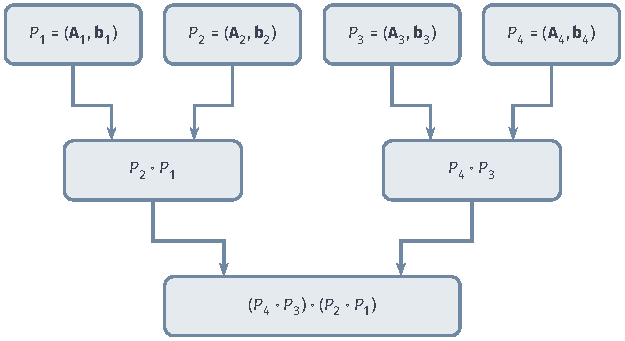
\includegraphics[width=105.791mm]{figures/05-neural-network-models/00-shared/tikz/rnn-scan/figure.pdf}
  \caption{仿射状态更新的有序组合。四个单步变换先组成两个连续片段，再组成整段；$Q\circ P$表示先执行$P$再执行$Q$。平衡组合树展示的是扫描中的汇总阶段，完整前缀扫描还要把此前片段的结果传给各位置，才能得到每步状态。树形计算可缩短依赖深度，但不改变输入顺序。}
  \label{fig:rnn-scan}
\end{figure}
\FloatBarrier

对逐坐标仿射更新，工作高效的扫描可用$O(Tm)$总运算量和$O(\log T)$组合深度得到前缀；稠密矩阵组合还要执行矩阵乘法，成本随状态宽度另行增加。普通RNN的非线性组合也通常无法保持固定大小、便于计算的仿射表示。可并行的条件是各步系数可提前取得、组合闭合且足够便宜；若系数必须由尚未计算的旧状态产生，就不能直接预先扫描。

\begin{example}[同一状态模型的递推与卷积]
  \label{ex:rnn-ssm-equivalence}
  取标量更新$h^{(t)}=\tfrac12 h^{(t-1)}+x_t$、$y_t=h^{(t)}$、$h^{(0)}=0$，输入为$(1,2,0)$。递推得到$(1,5/2,5/4)$。卷积核为$(1,1/2,1/4,\ldots)$，故第三步输出为$0+\tfrac12\times2+\tfrac14\times1=5/4$。整段训练可以按卷积组织，逐步预测可以按状态组织；相同输出来自相同模型的代数等价，而不是两套分别训练的参数。
\end{example}

\subsection{HiPPO}
\label{sec:rnn-hippo}

前面的线性框架解决了“怎么算”，却没有回答一个更根本的问题：状态里到底\emph{该存什么}，才能用有限的$m$个数最好地概括整段历史？随意选一个状态矩阵并不能保证它保留了远期信息。\term{高阶多项式投影}（high-order polynomial projection operators, HiPPO）把“记忆”显式定义成一个在线近似问题：\emph{用$m$个随时间更新的系数，去逼近到目前为止的整段历史函数，使加权平方误差最小}。相比只存一个滑动平均，多个基函数系数可以分别刻画历史的平均水平、变化趋势、曲率等不同形态\scite{gu2020hippo}。这个投影思路给出的更新矩阵，后来成为S4初始化状态动态的依据。

\subsubsection{投影系数保存什么}
\label{sec:rnn-hippo-memory}

设标量历史信号为$f(u)$，在当前时刻$\tau$选定历史权重测度$\mu_\tau$和相应正交归一基$p_0(u;\tau),\ldots,p_{m-1}(u;\tau)$。在该测度下平方可积时，投影系数与近似信号为
\begin{equation}
  c_i(\tau)=\int f(u)p_i(u;\tau)\,\mathrm{d}\mu_\tau(u),
  \qquad
  \widehat f_\tau(u)=\sum_{i=0}^{m-1}c_i(\tau)p_i(u;\tau)\text{。}
  \label{eq:rnn-hippo-projection}
\end{equation}
它在所选$m$维基函数空间中最小化加权平方误差。状态记录这组基函数系数；每个系数汇集一个历史形状的影响，权重与有限基函数数目共同决定可保留的细节。

\subsubsection{在线更新与网络组织}
\label{sec:rnn-hippo-architecture}

例如缩放Legendre版本在$[0,\tau]$上采用均匀权重，将整个历史区间缩放到固定区间上的Legendre多项式。
这里采用归一化的均匀测度，使整个区间的总权重为1。前两个基函数具体为
\[
  \begin{aligned}
    \mathrm d\mu_\tau(u)
      &=\frac{\mathbf{1}_{[0,\tau]}(u)}{\tau}\,\mathrm du,\\
    p_0(u;\tau)&=1,\\
    p_1(u;\tau)&=\sqrt3\left(\frac{2u}{\tau}-1\right)\text{。}
  \end{aligned}
\]
更高阶可取$p_i(u;\tau)=\sqrt{2i+1}\,P_i(2u/\tau-1)$，其中$P_i$是$[-1,1]$上满足$P_i(1)=1$的Legendre多项式。换元$z=2u/\tau-1$后，测度变为$\mathrm dz/2$；Legendre多项式在该测度下的平方积分为$1/(2i+1)$，因此因子$\sqrt{2i+1}$把每个基的范数归一到1，不同阶仍正交。

投影定义给出了任一时刻的系数，在线更新还要回答：区间从$[0,\tau]$略微延长后，怎样只用旧系数和新端点值更新它们。我们先取$m=2$看清这一步。为直接使用通常的Leibniz积分求导法则，以下走查暂设$f$连续，并始终取$\tau>0$；连续性是此处求导采用的条件，比定义投影时的平方可积条件更强。将前两个基代入投影式，有
\[
  \begin{aligned}
    c_0(\tau)&=\frac1\tau\int_0^\tau f(u)\,\mathrm du,\\
    c_1(\tau)&=\frac{\sqrt3}{\tau}
      \int_0^\tau f(u)\left(\frac{2u}{\tau}-1\right)\,\mathrm du\text{。}
  \end{aligned}
\]
求导时有三种变化需要分开：积分区间增加了新端点，归一化权重$1/\tau$改变，基函数也随区间长度改变。对$i=0,1$，把这三项分别写出便是
\[
  \begin{aligned}
    \frac{\mathrm dc_i}{\mathrm d\tau}
      &=\frac{f(\tau)p_i(\tau;\tau)}{\tau}
        -\frac{c_i(\tau)}{\tau}\\
      &\quad+\frac1\tau\int_0^\tau
        f(u)\frac{\partial p_i(u;\tau)}{\partial\tau}\,\mathrm du\text{。}
  \end{aligned}
\]
$p_0$不随$\tau$变化，而$p_1(\tau;\tau)=\sqrt3$、$\partial p_1(u;\tau)/\partial\tau=-2\sqrt3\,u/\tau^2$，所以
\[
  \begin{aligned}
    \frac{\mathrm dc_0}{\mathrm d\tau}
      &=\frac{f(\tau)-c_0(\tau)}{\tau},\\
    \frac{\mathrm dc_1}{\mathrm d\tau}
      &=\frac{\sqrt3 f(\tau)-c_1(\tau)}{\tau}
        -\frac{2\sqrt3}{\tau^3}\int_0^\tau u f(u)\,\mathrm du\text{。}
  \end{aligned}
\]
第二行还含一阶历史矩；但它已经包含在$c_0,c_1$中，无需保存整个历史来重新积分。由$c_1$的积分表达式整理可得
\[
  \begin{aligned}
    c_1(\tau)
      &=\frac{2\sqrt3}{\tau^2}\int_0^\tau u f(u)\,\mathrm du
        -\sqrt3 c_0(\tau),\\
    \frac{2\sqrt3}{\tau^3}\int_0^\tau u f(u)\,\mathrm du
      &=\frac{c_1(\tau)+\sqrt3 c_0(\tau)}{\tau}\text{。}
  \end{aligned}
\]
代回后，两个系数的更新闭合为
\[
  \begin{aligned}
    \frac{\mathrm dc_0}{\mathrm d\tau}
      &=\frac{f(\tau)-c_0(\tau)}{\tau},\\
    \frac{\mathrm dc_1}{\mathrm d\tau}
      &=\frac{\sqrt3 f(\tau)-\sqrt3 c_0(\tau)-2c_1(\tau)}{\tau}\text{。}
  \end{aligned}
\]
新端点提供当前输入项，权重和基的变化共同产生旧系数项；其中$c_0$进入$c_1$的更新，正是移动基带来的系数耦合。更高阶也可用基函数关系把求导后出现的历史矩写回已有系数，得到下面的一般矩阵形式。

使用从零开始的$i,j\in\{0,\ldots,m-1\}$，其连续系数更新可写为
\begin{equation}
  \begin{aligned}
    \frac{\mathrm{d}\bm{c}(\tau)}{\mathrm{d}\tau}
      &=-\frac{1}{\tau}\bm{H}\bm{c}(\tau)
        +\frac{1}{\tau}\bm{b}f(\tau),\qquad \tau>0,\\
    H_{i,j}&=
      \begin{cases}
        \sqrt{(2i+1)(2j+1)},&i>j,\\
        i+1,&i=j,\\
        0,&i<j,
      \end{cases}
      \qquad b_i=\sqrt{2i+1}\text{。}
  \end{aligned}
  \label{eq:rnn-hippo-legs}
\end{equation}
随时间变化的$1/\tau$反映历史区间不断扩张，更新矩阵也随当前时间改变。$m=1$时，$c_0$是整个区间的均值，其导数为$(f(\tau)-c_0(\tau))/\tau$，这给出了系数更新的直观核验。离散实现需选择初始化和离散化，不能在$\tau=0$直接代入。

测度决定“哪些历史值得近似”：固定窗口强调近期区间，指数权重弱化久远输入，随时间扩张的均匀区间覆盖全部过去，但固定阶数的分辨率会受到区间增长影响。HiPPO提供状态构造原则和相应结构矩阵，完整预测网络仍需要输入变换、读出及学习目标。可以固定投影动态、学习前后变换，也可以以结构矩阵初始化后再调整；后者需要重新检查状态是否仍满足原来的投影含义。投影误差的性质不能直接代替任务泛化误差。


图~\ref{fig:rnn-hippo}展示了一种把投影记忆接入任务网络的方式。实际观测可先经过可学习映射形成$f(\tau)$；投影更新维护系数，任务读出利用系数产生预测。若输入有多个特征，可以为各通道分别维护一组系数，再混合通道。重构历史使用已选定的基函数，任务读出则由监督目标决定，两者用途不同。
\begin{figure}[htb]
  \centering
  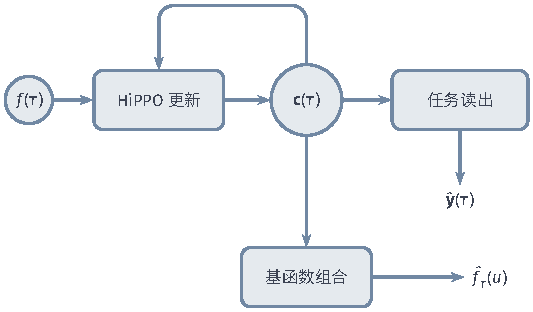
\includegraphics[width=90.293mm]{figures/05-neural-network-models/00-shared/tikz/rnn-hippo/figure.pdf}
  \caption{HiPPO投影记忆与任务网络的一种组合。反馈维护系数状态，读出产生任务预测；下方将同一系数与基函数组合，近似重构历史信号。HiPPO本身规定记忆表示及更新，图中的任务读出与输入特征映射可另行学习，并非唯一的HiPPO网络架构。}
  \label{fig:rnn-hippo}
\end{figure}
\FloatBarrier

若投影动态固定，任务损失训练输入映射和读出；输入映射可学习时，梯度仍需经过投影递推回到此前输入特征。若进一步训练投影矩阵，模型获得调整动态的自由，也放松了投影所规定的约束。固定投影动态维持了原来的投影约束，训练矩阵则让任务调整状态响应；参数范围决定当前模型保留哪种投影含义。

\subsubsection{历史覆盖与长期依赖的边界}
\label{sec:rnn-hippo-long-memory}

LegS把全部过去放进随时间扩张的区间，没有用一个固定窗口把早期输入直接删除。最低阶系数是均值：在$[0,\tau]$上，$c_0(\tau)=\tau^{-1}\int_0^\tau f(u)\,\mathrm du$。时刻$u$附近面积为$\varepsilon$的窄脉冲，对这个均值的贡献约为$\varepsilon/\tau$，随当前时刻按倒数减弱，而不是按已经经过的更新步数以固定比例反复衰减。

这个性质也可从状态更新看出。对$0<\sigma<\tau$，将$[\sigma,\tau]$间的输入固定，初始系数扰动满足
\begin{equation}
  \delta\bm c(\tau)
    =\exp\!\left[-\bm H\log(\tau/\sigma)\right]\delta\bm c(\sigma)\text{。}
  \label{eq:rnn-hippo-time-ratio}
\end{equation}
因为此区间的齐次更新是$\delta\dot{\bm c}=-\bm H\delta\bm c/\tau$，积分变量是$\log\tau$。与固定矩阵的$\exp(\bm A(\tau-\sigma))$相比，LegS按时间比值组织保留；最低阶模式的系数为$\sigma/\tau$。完整状态传播还包含其他模式及范数常数，任务梯度另经过输入映射和读出；最低阶模式只展示了时间比值的一个保留尺度。

前面用前两个基函数推得了在线更新；下面把同一组系数带回重构式，检验这份有限记忆怎样恢复历史的水平和趋势。

多个系数提供的不是多个历史位置，而是多个形状特征。取$p_0=1$、$p_1=\sqrt3(2u/\tau-1)$，对线性历史$f(u)=a+bu$，两个系数为
\begin{equation}
  c_0=a+\frac{b\tau}{2},\qquad c_1=\frac{b\tau}{2\sqrt3}\text{。}
  \label{eq:rnn-hippo-linear-example}
\end{equation}
代回基函数组合即可精确恢复这条线性函数：第一个系数保存水平，第二个补上趋势。若历史含有很多窄尖峰，两个系数便不足以定位每个尖峰；提高阶数增加分辨能力，也增加状态与计算成本。

因此，HiPPO把长期记忆转为有明确误差准则的在线压缩。它适合考察较长区间上的形状和趋势，固定阶数、有限精度、所选测度与信号变化共同限制可恢复细节。模型若需要精确取回任意久远符号，还需检验相应信息在投影后是否可区分；任务网络的非线性与读出同样可能带来额外学习困难。

\subsection{S4}
\label{sec:rnn-s4}

HiPPO给了一个有依据的状态矩阵，但直接拿来训练仍有两个工程障碍：一是状态矩阵是稠密的$m\times m$矩阵，逐步递推每步都要做$O(m^2)$的矩阵乘法，状态一宽就很贵；二是想用卷积视角并行训练时，需要生成长度为$T$的卷积核$\bm K_k=\bm C\overline{\bm A}^k\overline{\bm B}$，而稠密矩阵反复相乘、再加上HiPPO矩阵直接对角化的数值不稳定，使这个核难以快速且稳定地求得。\term{结构化状态空间序列模型}（structured state space sequence model, S4）的核心贡献，就是找到状态矩阵的一种特殊数学分解（对角加低秩），使得递推、卷积核生成都能在近线性的代价下稳定进行\scite{gu2022s4}。

这里的S4状态模块采用不随时间位置改变的连续矩阵$\bm A$，以保持前面卷积表达所必需的线性时不变条件。它借用HiPPO的结构矩阵和初始化思想；注意前面LegS的$-\bm H/\tau$仍随历史区间扩展而改变，不能直接把那条时变投影更新当作此处的固定动态。

\subsubsection{结构矩阵与核生成}
\label{sec:rnn-s4-structure}

我们以刚才的$\bm H$为例，追踪结构分解与坐标变换怎样相接。取固定矩阵$\bm A_0=-\bm H\in\mathbb R^{m\times m}$，另定义实向量$\bm p\in\mathbb R^m$，其分量为$(\bm p)_i=\sqrt{(2i+1)/2}$，下标仍从0开始。这里$\bm p$用于分解矩阵，与前面随$u$变化的多项式基$p_i(u;\tau)$是不同对象。补上一个秩一矩阵后，得到
\[
  \begin{aligned}
    \bm N&=\bm A_0+\bm p\bm p^{\top}
      =-\frac12\bm I+\bm S,\\
    S_{i,j}&=
      \begin{cases}
        -\tfrac12\sqrt{(2i+1)(2j+1)},&i>j,\\
        0,&i=j,\\
        \tfrac12\sqrt{(2i+1)(2j+1)},&i<j\text{。}
      \end{cases}
  \end{aligned}
\]
对角线上$-(i+1)+(2i+1)/2=-1/2$，非对角元则成对反号，因此$\bm S^{\top}=-\bm S$。于是$\bm N\bm N^*=\bm N^*\bm N=\bm I/4-\bm S^2$，$\bm N$是正规矩阵，可以用酉矩阵$\bm V\in\mathbb C^{m\times m}$对角化为$\bm N=\bm V\bm\Lambda\bm V^*$，其中$\bm V^*\bm V=\bm I$。这一步对角化的是补正后的$\bm N$，原来的状态矩阵仍为$\bm A_0=\bm N-\bm p\bm p^{\top}$。

在连续模型$\dot{\bm h}=\bm A_0\bm h+\bm B\bm x$、$\bm y=\bm C\bm h+\bm D\bm x$中，将同一状态改用坐标$\bm h'=\bm V^*\bm h$表示，并同步变换输入、输出映射：
\[
  \begin{aligned}
    \bm A'&=\bm V^*\bm A_0\bm V
      =\bm\Lambda-(\bm V^*\bm p)(\bm V^*\bm p)^*,\\
    \bm B'&=\bm V^*\bm B,\qquad
    \bm C'=\bm C\bm V\text{。}
  \end{aligned}
\]
由$\bm h=\bm V\bm h'$代回，得到$\dot{\bm h}'=\bm A'\bm h'+\bm B'\bm x$和$\bm y=\bm C'\bm h'+\bm D\bm x$；因此改变的是状态坐标，输入到输出的映射保持不变，直达项$\bm D$也不变。初态同样需变为$\bm h'(0)=\bm V^*\bm h(0)$。原来稠密的正规部分现在只需对角矩阵$\bm\Lambda$表示，余下两向量的外积秩至多为1；“低秩”在这里表示只用少数方向修正对角动态，因此可以用少量列向量保存这项修正。

这个例子在复坐标中的两个低秩因子都为$\bm V^*\bm p\in\mathbb C^{m\times1}$。原模型为实数时，可将复数谱和相应系数按共轭对组织，中间复数项组合后仍给出原来的实输出；在复坐标中直接学习参数时，也需保持相应的共轭配对或采用等价的实数表示。下面省去新坐标的撇号，并用$\bm P,\bm Q$允许秩为$r$的修正。

其关键结构之一是\term{对角加低秩}（diagonal plus low-rank, DPLR）：在合适的复数坐标系中写为
\begin{equation}
  \bm{A}=\bm{\Lambda}-\bm{P}\bm{Q}^{*}\text{，}
  \label{eq:rnn-s4-dplr}
\end{equation}
其中$\bm{\Lambda}\in\mathbb{C}^{m\times m}$是对角矩阵，$\bm{P},\bm{Q}\in\mathbb{C}^{m\times r}$，秩$r$较小，$*$表示共轭转置。这个坐标系来自正规矩阵加低秩结构的酉变换；正规矩阵$\bm{N}$满足$\bm{N}\bm{N}^{*}=\bm{N}^{*}\bm{N}$，其酉对角化避免任意病态基变换，加入低秩项后的$\bm{A}$则不必正规。输入和输出映射也随坐标一起变换，实际输出可通过共轭配对保持实数。

前面的零阶保持规则在输入区间保持常值时精确积分连续动态。这里改用另一种离散化：在一个长度为$\Delta$的区间内，以首末状态的平均值近似状态项的积分，输入仍取本区间的常值$\bm x_t$，即
\[
  \bm h^{(t)}-\bm h^{(t-1)}
    \approx\frac{\Delta}{2}\bm A
       \left(\bm h^{(t)}+\bm h^{(t-1)}\right)
       +\Delta\bm B\bm x_t\text{。}
\]
把这条梯形近似作为离散更新的定义，再将含新状态的项移到左侧，可得精确的代数关系
\[
  \left(\bm I-\frac{\Delta}{2}\bm A\right)\bm h^{(t)}
    =\left(\bm I+\frac{\Delta}{2}\bm A\right)\bm h^{(t-1)}
       +\Delta\bm B\bm x_t\text{。}
\]
当左侧矩阵可逆时，左乘其逆即可得到下面的状态转移与写入矩阵。这种有理矩阵形式把所需计算转为线性矩阵的求逆作用，便于继续使用对角加低秩结构。

S4采用的双线性离散化为
\begin{equation}
  \begin{aligned}
    \overline{\bm{A}}&=
      (\bm{I}-\tfrac{\Delta}{2}\bm{A})^{-1}
      (\bm{I}+\tfrac{\Delta}{2}\bm{A}),\\
    \overline{\bm{B}}&=
      (\bm{I}-\tfrac{\Delta}{2}\bm{A})^{-1}\Delta\bm{B}\text{，}
  \end{aligned}
  \label{eq:rnn-s4-bilinear}
\end{equation}
需保证逆矩阵存在。DPLR形式使相关逆矩阵作用可以通过对角运算和低秩修正计算；固定秩时，一步递推可达到$O(m)$量级，而不是稠密状态转移的$O(m^2)$。

两种离散化在有限步长下一般给出不同参数。例如对零输入的标量衰减$A=-1$，取$\Delta=1$，零阶保持得到$\overline A=e^{-1}\approx0.368$，双线性规则则得到$\overline A=(1-1/2)/(1+1/2)=1/3$。两者都描述衰减，但只有前者在这里等于该保持区间的精确连续解；后续的递推、卷积和核生成必须使用各自离散规则给出的同一套参数。

核生成也利用这套结构。计算路线是先在$T$个单位根处求一个有限多项式的值，再用逆DFT恢复它的$T$个系数；这些系数就是所需的卷积核。把长度为$T$的核视为一个有限多项式，用几何和恒等式可写为
\begin{equation}
  \begin{aligned}
    \bm{G}_T(z)&=\sum_{k=0}^{T-1}\bm{K}_k z^k\\
      &=\bm{C}\left[\bm{I}-(z\overline{\bm{A}})^T\right]
         (\bm{I}-z\overline{\bm{A}})^{-1}\overline{\bm{B}}\text{，}
  \end{aligned}
  \label{eq:rnn-s4-generating-function}
\end{equation}
第二行适用于所写逆矩阵存在时，$T$表示有限核长度，矩阵上的$T$是幂次而非转置。要看清这个逆怎样利用DPLR结构，下面固定单输入单输出情形，记$\bm B=\bm b$、$\bm C=\bm c^*$，其中$\bm b,\bm c\in\mathbb C^m$；此时$\bm G_T$退化为标量多项式$G_T$，低秩$r$不随$m,T$增长。

由双线性离散化，
\[
  \bm I-z\overline{\bm A}
    =(\bm I-\tfrac{\Delta}{2}\bm A)^{-1}
      \left[(1-z)\bm I-\frac{\Delta}{2}(1+z)\bm A\right]\text{。}
\]
对$z\neq-1$，提出方括号中的系数，可将离散逆矩阵作用改写为
\begin{equation}
  \begin{aligned}
    \xi(z)&=\frac{2}{\Delta}\frac{1-z}{1+z},\\
    (\bm I-z\overline{\bm A})^{-1}\overline{\bm b}
      &=\frac{2}{1+z}(\xi(z)\bm I-\bm A)^{-1}\bm b\text{。}
  \end{aligned}
  \label{eq:rnn-s4-resolvent}
\end{equation}
其中$\overline{\bm b}=(\bm I-\Delta\bm A/2)^{-1}\Delta\bm b$。右侧的$(\xi\bm I-\bm A)^{-1}$称为预解矩阵（resolvent）。双线性变换把离散频率点$z$转为连续状态矩阵的频率变量$\xi$，上式仍以相关逆存在为前提。

核只保留有限长度，因此求值还带有截断因子。在$T$个单位根
$z_\ell=\exp(-2\pi\mathrm i\ell/T)$、$\ell=0,\ldots,T-1$上，$\mathrm i$为虚数单位，$z_\ell^T=1$，因此可以共用修正后的输出行
\begin{equation}
  \bm c_T^*=\bm c^*(\bm I-\overline{\bm A}^{T})\text{。}
  \label{eq:rnn-s4-finite-readout}
\end{equation}
代入式\eqref{eq:rnn-s4-generating-function}与式\eqref{eq:rnn-s4-resolvent}，对$z_\ell\neq-1$得到
\begin{equation}
  G_T(z_\ell)=\frac{2}{1+z_\ell}
    \bm c_T^*(\xi(z_\ell)\bm I-\bm A)^{-1}\bm b\text{。}
  \label{eq:rnn-s4-root-evaluation}
\end{equation}
这里利用$z^T=1$才把修正行统一为$\bm c_T^*$；一般$z$处仍须保留$\bm I-(z\overline{\bm A})^T$，修正项与$\bm I-\overline{\bm A}^T$在一般求值点上不同。

现在代入$\bm A=\bm\Lambda-\bm P\bm Q^*$。记$\lambda_j$为$\bm\Lambda$的第$j$个对角元素，并令
\[
  \bm R_\xi=(\xi\bm I-\bm\Lambda)^{-1}
    =\operatorname{diag}\!\left(
       \frac1{\xi-\lambda_1},\ldots,\frac1{\xi-\lambda_m}\right)\text{。}
\]
Woodbury恒等式把原来的$m\times m$逆化为对角逆和一个$r\times r$逆：
\begin{equation}
  (\xi\bm I-\bm A)^{-1}
    =\bm R_\xi-\bm R_\xi\bm P
       (\bm I_r+\bm Q^*\bm R_\xi\bm P)^{-1}
       \bm Q^*\bm R_\xi\text{。}
  \label{eq:rnn-s4-woodbury}
\end{equation}
将其代入式\eqref{eq:rnn-s4-root-evaluation}，只需计算
$\bm c_T^*\bm R_\xi\bm b$、$\bm c_T^*\bm R_\xi\bm P$、
$\bm Q^*\bm R_\xi\bm b$和$\bm Q^*\bm R_\xi\bm P$，再作小矩阵求逆与乘法。每个对象的元素都是如下形式的求和：
\begin{equation}
  \bm u^*\bm R_\xi\bm v
    =\sum_{j=1}^{m}\frac{\overline{u_j}v_j}{\xi-\lambda_j}\text{，}
  \label{eq:rnn-s4-cauchy-sum}
\end{equation}
其中$\bm u$取$\bm c_T$或$\bm Q$的列，$\bm v$取$\bm b$或$\bm P$的列，$\overline{u_j}$表示复共轭。求和中的倒数因子$1/(\xi(z_\ell)-\lambda_j)$就是\term{Cauchy核}（Cauchy kernel）。因此加速的对象是许多频率点共享谱参数的这组求和，而不是为每个频率重新求一个一般稠密逆矩阵。

上述分解要求$\xi\bm I-\bm\Lambda$及低秩修正中的逆存在。若某个采样点使中间表达式奇异，应回到有限多项式求值，或使用已消去可去奇点的等价形式。偶数$T$还会包含$z_{T/2}=-1$，此点的$\xi$表达式有奇点；由$\bm I+\overline{\bm A}=2(\bm I-\Delta\bm A/2)^{-1}$可单独得到
\[
  G_T(-1)=\frac{\Delta}{2}\bm c_T^*\bm b
  \qquad(T\text{为偶数})\text{。}
\]
取得全部$T$个单位根处的值后，逆DFT恢复长度为$T$的核系数，可用FFT实现。这里保留的是有限多项式的值，不是无限序列频率响应的直接采样。

固定秩下，逐点直接执行式\eqref{eq:rnn-s4-cauchy-sum}仍需$O(mT)$求和工作，形成$\bm c_T$也有成本；上述恒等式本身并未证明近线性核生成。原始S4在相应快速结构算法下给出关于$m+T$的近线性分析，具体算法与数值实现仍需另行核对。得到核后，LTI状态模块可用适当补零的FFT卷积处理整段序列，单通道卷积的成本为$O(T\log T)$，核生成还包含前述结构求值与修正读出的工作。逐步预测改用同一组离散参数递推，无需保存全部历史输入。

\subsubsection{完整层、训练与逐步预测}
\label{sec:rnn-s4-architecture}

一个标量SSM只完成一条序列上的线性变换。完整S4层可为$d$个输入通道各设一个$m$维状态模块，得到$\bm y_t\in\mathbb R^d$，再作非线性变换和逐位置通道混合，例如
\begin{equation}
  \bm u_t=\bm M\,\phi(\bm y_t)+\bm b_{\mathrm{mix}},
  \qquad\bm M\in\mathbb R^{d\times d}\text{。}
  \label{eq:rnn-s4-channel-layer}
\end{equation}
$\phi$逐坐标作用，$\bm u_t$是本层输出特征，可送入下一层或任务头。维度匹配时还可以加入跨层残差与归一化。时间模块传播各通道的历史，通道混合再使不同特征相互作用；多个这样的层构成非线性序列网络。

图~\ref{fig:rnn-s4}把同一层的两种计算方式并列。整段输入已经给定时，由结构参数生成因果卷积核，再对各通道计算卷积；逐步预测时，维护各通道状态并直接递推。外部非线性与通道映射相同，切换的是线性状态模块的计算形式。
\begin{figure*}[htb]
  \centering
  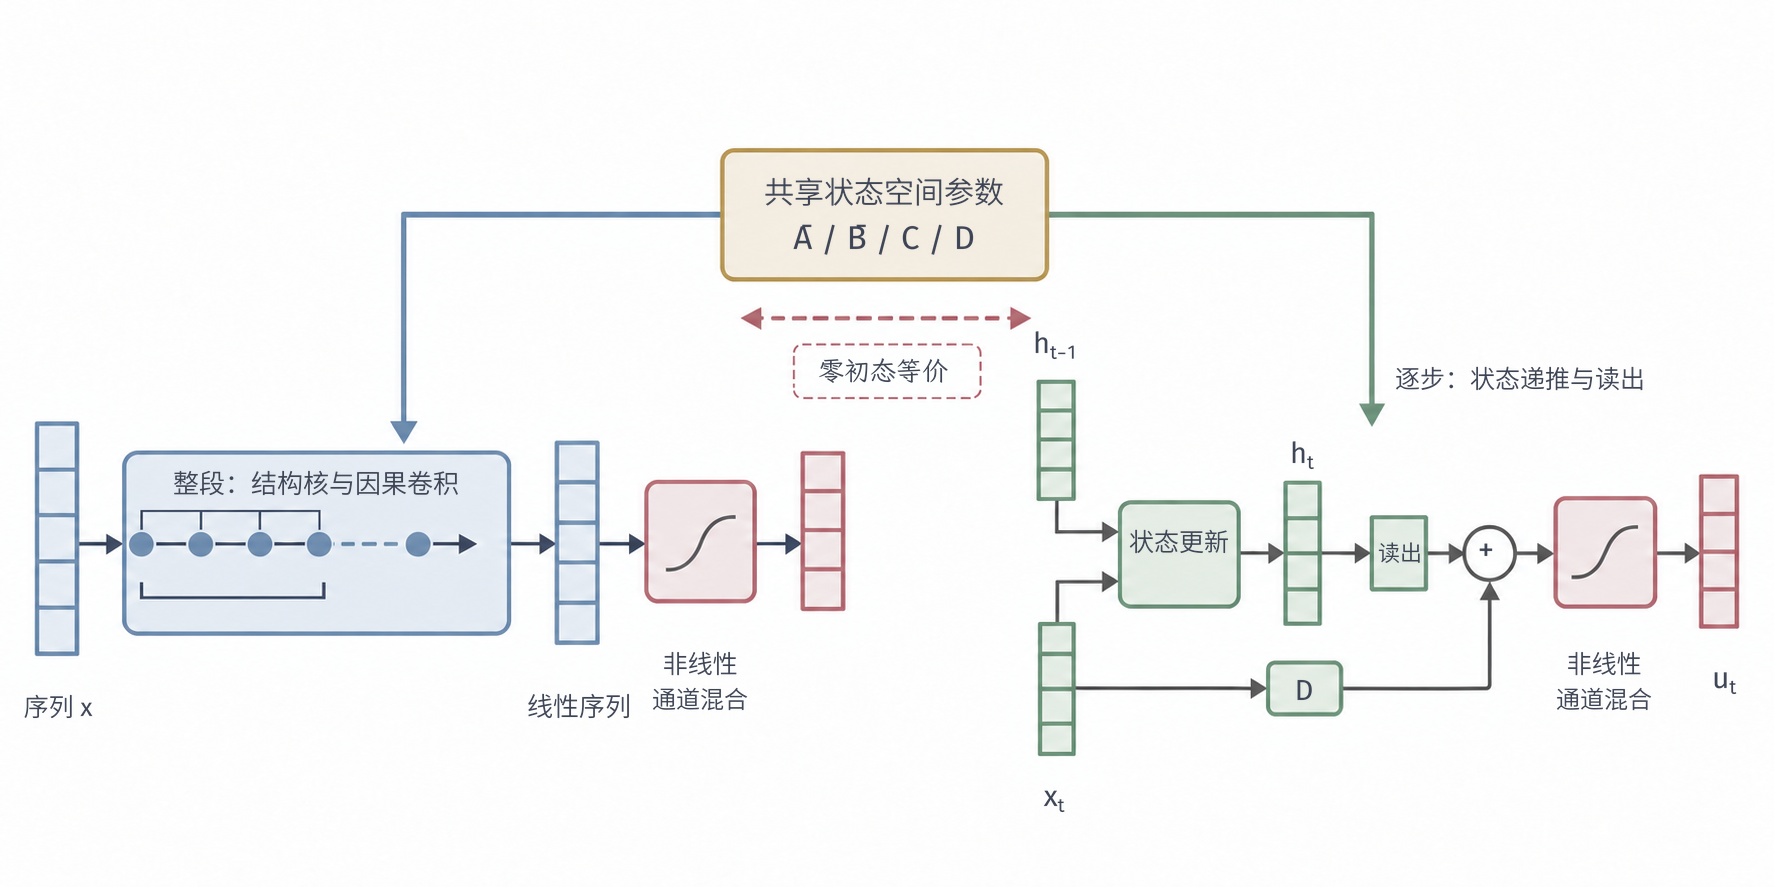
\includegraphics[width=150.199mm]{figures/05-neural-network-models/00-shared/generated/rnn-s4/figure.png}
  \caption{S4层的整段与逐步计算。两个路径共享同一组离散状态参数及后续通道映射，上方路径提供共享参数，跨路径虚线说明零初态下的等价关系。整段分支把直达映射$\bm D$并入零滞后卷积系数，$\widetilde{\bm K}_0=\bm K_0+\bm D$，其余滞后系数不变。零初态时，因果卷积与递推得到相同线性序列输出；非零初态需要补上对应初态响应。图中$\bm u$是层输出特征，任务预测还需相应读出。}
  \label{fig:rnn-s4}
\end{figure*}
\FloatBarrier

结构参数、输入输出映射、步长与通道映射由任务损失联合学习。卷积路径的反向计算对结构参数所生成的同一个核求导；预测切到递推时，需要使用与训练一致的离散化、因果约定和初始化。整个网络可以非线性，卷积等价只针对满足LTI条件的状态模块。

HiPPO-LegS的$1/\tau$更新与S4中的固定结构动态也应分清。S4借用结构矩阵和初始化思想，使网络可以学习有用的时间响应；当前模块的固定动态与LegS随历史区间扩展的更新有不同的时间含义。DPLR结构首先服务于高效计算，训练后的稳定性与长期响应还要检查参数取值。

\subsubsection{时间尺度与长期依赖}
\label{sec:rnn-s4-long-memory}

S4保存多久，与离散状态矩阵的模式有关。在可对角化情形下，$\bm K_k=\bm C\overline{\bm A}^k\overline{\bm B}$是多个指数模式的加权组合。某模式的特征值$\bar\lambda_j$满足$0<|\bar\lambda_j|<1$时，其幅度按$|\bar\lambda_j|^k$衰减，相应以步数计的时间尺度为
\begin{equation}
  \tau_{\mathrm{steps},j}=-\frac{1}{\log|\bar\lambda_j|}\text{。}
  \label{eq:rnn-s4-timescale}
\end{equation}
幅度经过这个步数约降到原来的$e^{-1}$。接近1的模式保留较久，较小的模式强调近期；复数模式还可表示振荡。不同时间尺度共同形成历史响应，输入映射决定往哪些模式写入，输出映射决定哪些模式参与预测。

对连续特征值$\lambda_j$，双线性离散化给出$\bar\lambda_j=(1+\Delta\lambda_j/2)/(1-\Delta\lambda_j/2)$。左半平面的特征值映入单位圆内，步长又改变离散时间尺度。特征值只描述模式，非正规矩阵的短期放大与数值条件仍需考虑；结构可高效计算，也不代表任意自由参数都稳定。

长期影响在输入输出层面写为$\partial\bm y_t/\partial\bm x_s=\bm K_{t-s}$，$s<t$；当前输入的导数还包含直接项$\bm D$。卷积路径直接计算这个历史响应，训练时不必按普通RNN的非线性单元逐步展开；但FFT与递推计算的是同一个映射，相关历史响应的导数也相同。若核在相关距离已经衰减，早期证据仍然弱；若读写映射没有利用慢模式，长时间尺度也不会自动转成任务所需的记忆。

S4因而同时改善状态的结构设计和整段计算。固定LTI模块对同一滞后使用同一响应，适合学习多尺度时间关系，却不能在单个模块中按每次输入的内容改写保留率。非线性堆叠扩展了网络表达，按内容选择状态的另一种做法则是下面的Mamba。

\subsection{Mamba}
\label{sec:rnn-mamba}

S4用固定的线性时不变动态换来了并行与长记忆，但“固定”也意味着它对所有输入一视同仁：无论当前内容是无关紧要的停用词还是需要牢记的关键事实，状态都按\emph{同一个}预设速率衰减和响应。可在真实语言中，需要记住的信息出现位置并不固定，理想的遗忘速度应\emph{随内容变化}——这正是LSTM门控解决过的问题，但LSTM又无法享受SSM的并行扫描。Mamba要把两者的优点合起来：\emph{让S4的部分系数由当前输入动态产生（选择性），同时保持状态更新对旧状态是仿射的，从而仍能用扫描并行}。\term{Mamba}让输入决定每一步的有效步长、写入和读出，改变哪些内容被写入、保留或读出。本节采用原始Mamba架构\scite{gu2023mamba}

\subsubsection{选择性状态更新}
\label{sec:rnn-mamba-selection}

为看清选择性，考察预处理后一个通道的标量输入$x_t$与$m$维状态。固定可学习的连续对角矩阵$\bm A$，由当前输入特征产生$\Delta_t>0$、$\bm B_t\in\mathbb R^m$和$\bm C_t\in\mathbb R^{1\times m}$，采用零阶保持时
\begin{equation}
  \begin{aligned}
    \overline{\bm A}_t&=\exp(\Delta_t\bm A),\\
    \overline{\bm B}_t&=\int_0^{\Delta_t}\exp(u\bm A)\bm B_t\,\mathrm du,\\
    \bm h^{(t)}&=\overline{\bm A}_t\bm h^{(t-1)}+\overline{\bm B}_t x_t,\\
    y_t&=\bm C_t\bm h^{(t)}+D x_t\text{。}
  \end{aligned}
  \label{eq:rnn-mamba-selection}
\end{equation}
$D$是通道的直接输入系数。输入相关不要求$\bm A$每步重新生成，选择性来自步长、写入和读出映射。多个通道各有状态，并由通道投影组合。

常用参数化令$A_{i,i}=-\exp(a_i)$、$\Delta_t=\operatorname{softplus}(d_t)$，其中$a_i$是参数，$d_t$由输入映射并加入偏置产生。这分别限制连续模式的衰减方向与步长的正值。$\bm B_t$决定输入写入哪些状态坐标，$\bm C_t$决定本步从哪些坐标形成输出。离散化是模型定义的一部分，复现时需核对写入项采用的具体规则。

取标量特例$A=-1$、$B_t=1$、$D=0$，更新成为
\begin{equation}
  h^{(t)}=e^{-\Delta_t}h^{(t-1)}+(1-e^{-\Delta_t})x_t\text{。}
  \label{eq:rnn-mamba-gate-special-case}
\end{equation}
小步长主要保留旧状态，大步长更多采用当前输入。这与控制门有明确联系，但完整模块具有多个状态坐标及输入相关的读写映射，其读写自由度由完整状态和各选择映射共同确定。

\subsubsection{完整模块的两条分支}
\label{sec:rnn-mamba-architecture}

选择性SSM只负责时间方向的状态计算。图~\ref{fig:rnn-mamba}把它放回完整模块：输入归一化与投影后分成两条支路，一条经过短因果卷积和SiLU，产生送入SSM的特征；另一条经过SiLU形成调制向量。SSM输出与调制向量逐坐标相乘，再经过输出投影和残差相加。

本例的归一化在每个样本、每个位置的特征坐标内计算，只根据当前位置的特征形成所需统计量，不把其他时间位置的值合入统计范围。整段训练时也逐位置应用同一规则，因此该步骤不会读取未来输入；下面的短卷积和选择性状态更新再按因果顺序处理时间依赖。
\begin{figure*}[htb]
  \centering
  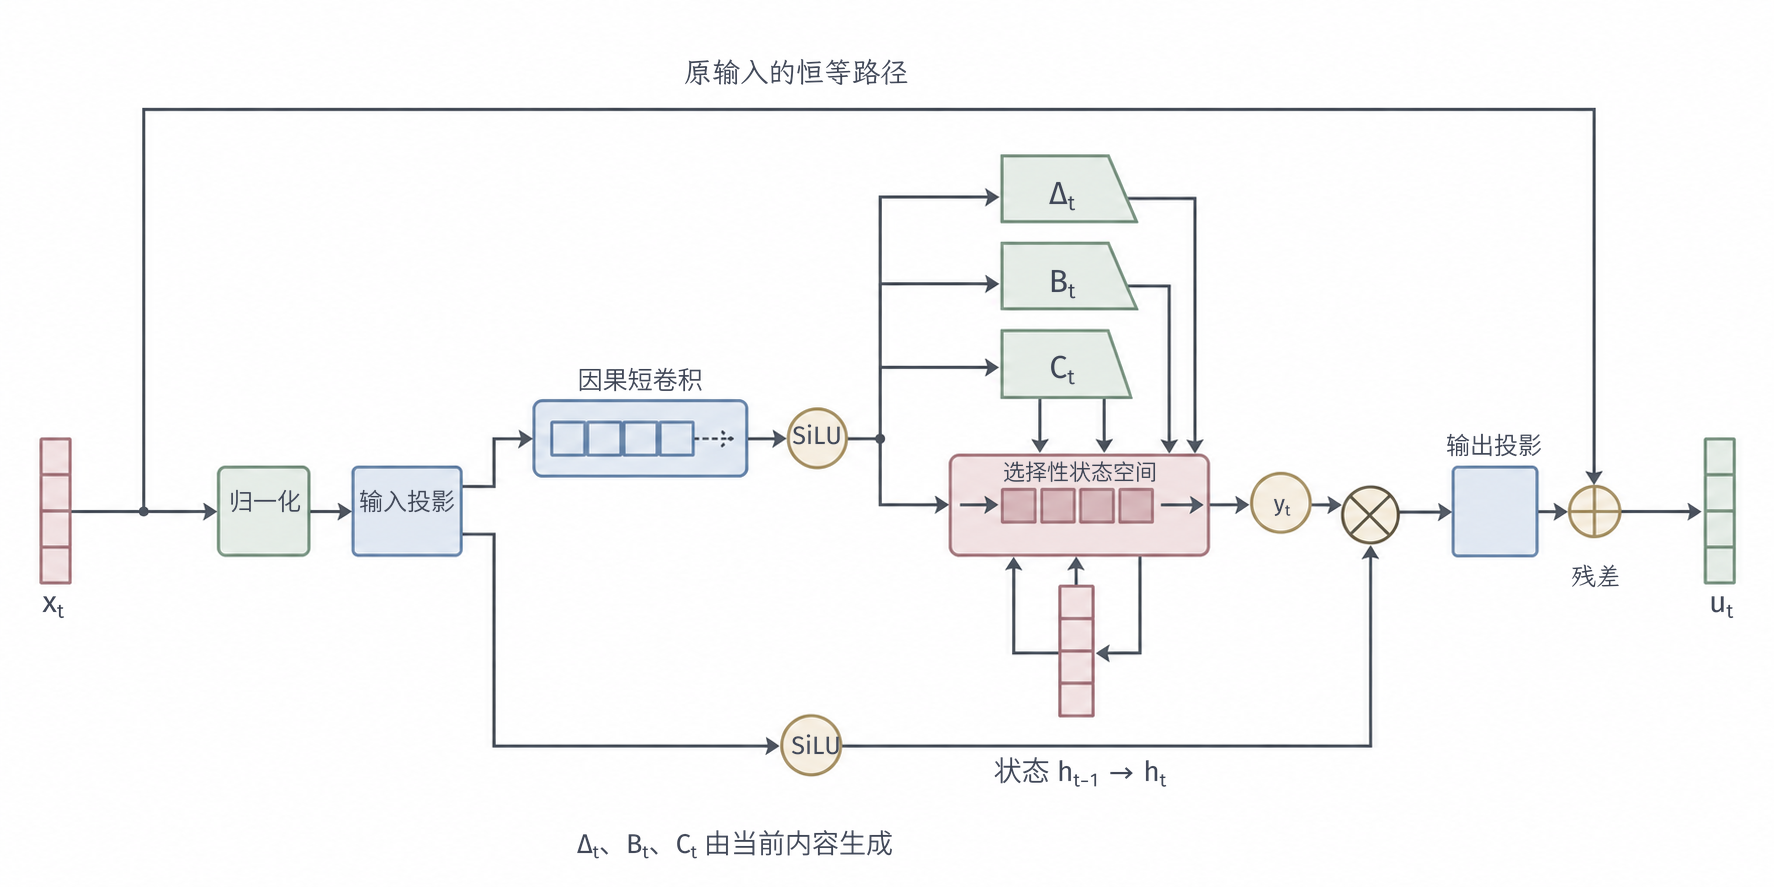
\includegraphics[width=150.199mm]{figures/05-neural-network-models/00-shared/generated/rnn-mamba/figure.png}
  \caption{原始Mamba模块的主要计算路径。选择参数分支说明选择性的来源：短卷积后的输入特征生成$\Delta_t,\bm B_t,\bm C_t$，并据此调节SSM更新；另一路特征调制SSM输出，上方直达线完成跨层残差。$\bm u_t$是模块输出，任务预测由后续网络读出。图中省略短卷积缓存、批次维和跨通道广播细节。}
  \label{fig:rnn-mamba}
\end{figure*}
\FloatBarrier

令归一化输入为$\widetilde{\bm x}_t\in\mathbb R^d$，内部通道数为$d_{\mathrm{in}}$，可将这两条支路写为
\begin{equation}
  \begin{aligned}
    \bm v_t&=\operatorname{SiLU}\!\left(\operatorname{CausalConv}
                (\bm W_{\mathrm v}\widetilde{\bm x})_t\right),\\
    \bm z_t&=\operatorname{SiLU}(\bm W_{\mathrm z}\widetilde{\bm x}_t),\\
    \bm y_t&=\operatorname{SelectiveSSM}(\bm v_{1:t}),\\
    \bm u_t&=\bm x_t+\bm W_{\mathrm{out}}(\bm y_t\odot\bm z_t)\text{。}
  \end{aligned}
  \label{eq:rnn-mamba-block}
\end{equation}
$\bm W_{\mathrm v},\bm W_{\mathrm z}\in\mathbb R^{d_{\mathrm{in}}\times d}$，$\bm W_{\mathrm{out}}\in\mathbb R^{d\times d_{\mathrm{in}}}$。各通道的选择系数由$\bm v_t$产生，$\bm y_t,\bm z_t$均为内部通道向量。SiLU调制支路缩放本步输出，其系数并未限制到$[0,1]$；时间记忆的保留率则来自SSM中的步长与状态参数。短卷积补充局部上下文，残差提供层方向的直达路径，各自作用不同。

\subsubsection{扫描、学习与计算代价}
\label{sec:rnn-mamba-scan}

输入相关系数使响应依赖具体输入和绝对位置，一般不能继续使用一个固定卷积核。不过，整段输入给定后，各步系数可先从输入计算；状态更新对旧状态仍是仿射的，对角结构又使组合便宜，所以能够使用式\eqref{eq:rnn-affine-composition}的扫描。若系数还依赖尚未算出的旧状态，就不能直接套用这种预先形成各步变换的方式，这也是它与一般LSTM／GRU计算组织的差别。

硬件感知的选择性扫描把离散化与状态更新放在适当存储层次中计算，避免在较慢存储中显式写出所有通道、所有位置的扩展状态；反向时可以重算中间量。扫描与重算改变计算顺序和存储策略，任务损失仍对同一递推求导。输入输出投影、短卷积、选择映射、状态参数与步长参数共同学习，选择哪些输入不是人工指定的必然结果。

设内部通道数为$d_{\mathrm{in}}$、每通道状态宽度为$m$，状态更新工作量为$O(Td_{\mathrm{in}}m)$，逐步持久状态为$O(d_{\mathrm{in}}m)$，还需短卷积和移位缓存。通道投影另有每步$O(dd_{\mathrm{in}})$成本。定长预测状态与高效整段扫描降低了计算负担，训练仍需优化器状态和相应反向信息，因此训练存储还随反向图、重算策略和优化器配置变化。

\subsubsection{有效时间与长期保留}
\label{sec:rnn-mamba-long-memory}

固定输入产生的系数，跨步状态扰动沿齐次路径传播为
\begin{equation}
  \frac{\partial\bm h^{(t)}}{\partial\bm h^{(s)}}
    =\exp\!\left(\bm A\sum_{u=s+1}^{t}\Delta_u\right)\text{，}
  \label{eq:rnn-mamba-memory-product}
\end{equation}
因为同一对角矩阵的指数可以相乘后合并。传播尺度由累计的内部步长决定：遇到无关输入时，若模型产生小$\Delta_u$，经过很多位置也可以只积累较少衰减；需要更新时再加大步长，并通过$\bm B_u$写入新内容。这将固定的逐步衰减变成内容相关的“有效经过时间”。

仍用式\eqref{eq:rnn-mamba-gate-special-case}作构造例子：从零状态读入$x_1=1$，取$\Delta_1=\log2$，得到$h^{(1)}=1/2$。其后100步输入为零且步长均为$0.001$，末状态为$(1/2)e^{-0.1}\approx0.452$。这个例子展示小步长如何弱化中间位置的遗忘；真实任务还要学到哪些位置应如此处理，且写入项的大小同时受$\bm B_t$和输入影响。

选择性更新把历史概括为定长状态。$\bm C_t$读取这些状态坐标，逐位置注意力则另存过去表示供本次查询评分；状态容量、输入干扰与有限精度仍限制可区分历史。系数对输入的导数、层间非线性和调制支路也进入完整梯度。选择机制提供了保留和覆盖的自由，扫描使这种机制便于计算，实际长期读取能力由保留规则、有限状态容量与任务学习共同决定。

% 完整作者列表较长，保留足够空间容纳本节开头的边注文献。
\Needspace{105mm}
\subsection{RWKV}
\label{sec:rnn-rwkv}

Mamba用选择性扫描获得了内容相关的记忆与并行性，RWKV则从另一个角度追求同样的目标：能否构造一个\emph{形式上完全是线性递推、只靠定长状态就能逐步生成}的模型，同时又像注意力那样让历史值的权重由“内容相似度”和“时间远近”共同决定？这样既保留RNN推理时状态恒定、显存不随序列变长的优点，又能在训练时把递推展开成可并行的加权求和。\term{接收门加权键值网络}（receptance weighted key value, RWKV）以时间混合和通道混合两种操作构成模块：历史值由内容权重与时间衰减共同累积成两个向量状态，再由一个接收门控制输出多少。本节采用2023年论文中的RWKV-4形式；后续版本的状态形状和更新可能不同\scite{peng2023rwkv}

\subsubsection{时间混合与加权状态}
\label{sec:rnn-rwkv-time-mixing}

设时间混合子模块的输入为$\bm{x}_t\in\mathbb{R}^{d}$，在完整层中它已由\term{层归一化}（layer normalization, LN）得到。这里LN只对同一位置的$d$个特征坐标计算均值与方差，标准化后再作可学习的逐坐标缩放和平移，各位置共享这些参数；具体公式见式\eqref{eq:transformer-layernorm}。它不跨样本或时间位置统计，因此归一化本身不会读取未来输入。时间混合先在当前与前一步输入之间逐坐标混合，再投影为键、值和接收向量：
\begin{equation}
  \bm{a}_t=\bm{W}_{\mathrm{a}}\!\left(
    \bm{\mu}_{\mathrm{a}}\odot\bm{x}_t
    +(\bm{1}-\bm{\mu}_{\mathrm{a}})\odot\bm{x}_{t-1}\right),
  \quad \mathrm{a}\in\{\mathrm{k},\mathrm{v},\mathrm{r}\}\text{。}
  \label{eq:rnn-rwkv-time-mixing}
\end{equation}
其中$\bm{\mu}_{\mathrm{a}}\in\mathbb{R}^{d}$是可学习混合系数，$\bm{W}_{\mathrm{a}}\in\mathbb{R}^{d\times d}$；$\bm{k}_t,\bm{v}_t,\bm{r}_t$分别取$\bm{a}_t$的对应结果。序列起始时的前一步输入需按约定初始化。

所有指数、除法和乘积按坐标进行。令非负衰减参数为$\bm{w}\in\mathbb{R}^{d}$，当前项偏置为$\bm{u}\in\mathbb{R}^{d}$，历史分子和分母状态初值为零，则
\begin{equation}
  \begin{aligned}
    \bm{v}_{\mathrm{agg}}^{(t)}&=
      \frac{\bm{a}^{(t-1)}+e^{\bm{u}+\bm{k}_t}\odot\bm{v}_t}
           {\bm{b}^{(t-1)}+e^{\bm{u}+\bm{k}_t}},\\
    \bm{a}^{(t)}&=e^{-\bm{w}}\odot\bm{a}^{(t-1)}
                    +e^{\bm{k}_t}\odot\bm{v}_t,\\
    \bm{b}^{(t)}&=e^{-\bm{w}}\odot\bm{b}^{(t-1)}+e^{\bm{k}_t},\\
    \bm{o}_t&=\bm{W}_{\mathrm{o}}\!\left(
      \operatorname{sigmoid}(\bm{r}_t)\odot\bm{v}_{\mathrm{agg}}^{(t)}\right)\text{。}
  \end{aligned}
  \label{eq:rnn-rwkv-recurrence}
\end{equation}
输出在历史状态更新前读取旧累积量，并为当前项使用$\bm{u}$；之后写入状态的当前项不包含该偏置。展开分子可见，第$i<t$个位置的权重为$\exp(-(t-1-i)\bm{w}+\bm{k}_i)$。它取决于该位置的键和时间距离，接收门再决定每个通道输出多少，没有对每个历史位置重新计算查询—键点积。

可以用两个位置的计算区分“当前怎样读出”和“历史怎样保存”。只看一个通道，取$w=\log2$、$u=\log3$，两个位置的键均为零，值依次为$v_1=2$、$v_2=0$。第一步没有历史，聚合值为2，写入后$a^{(1)}=2,b^{(1)}=1$。第二步读出时，旧值的权重为1，当前值的权重为3，因此聚合值为$(2+3\times0)/(1+3)=1/2$。随后保存历史时，旧贡献衰减一半，当前贡献按权重1写入，得到$a^{(2)}=1,b^{(2)}=3/2$。这两个新状态留给下一步使用，不能用它们的比值替代本步的聚合值；本步还要经过接收门和输出投影，才得到$\bm o_t$。

状态递推证明了过去的加权和可以由两个向量维护，不必逐步保存全部键值。直接指数形式容易上溢，实际实现还维护尺度或最大值，使用重缩放保持与上述比值等价。分母在非空步由正指数项保证为正；数值实现需要这种重缩放来控制指数范围。

\subsubsection{通道混合与完整残差层}
\label{sec:rnn-rwkv-architecture}

时间混合负责历史累积，\term{通道混合}（channel mixing）则在当前表示中组合不同特征。它也用当前与前一步输入作混合，但不重复WKV的历史加权和。令相应子模块输入仍记为$\bm x_t\in\mathbb R^d$，可写为
\begin{equation}
  \begin{aligned}
    \bm k'_t&=\bm W'_{\mathrm k}\left(\bm\mu'_{\mathrm k}\odot\bm x_t
          +(\bm1-\bm\mu'_{\mathrm k})\odot\bm x_{t-1}\right),\\
    \bm r'_t&=\bm W'_{\mathrm r}\left(\bm\mu'_{\mathrm r}\odot\bm x_t
          +(\bm1-\bm\mu'_{\mathrm r})\odot\bm x_{t-1}\right),\\
    \bm o'_t&=\operatorname{sigmoid}(\bm r'_t)\odot
         \bm W'_{\mathrm v}\left(\operatorname{ReLU}(\bm k'_t)
                              \odot\operatorname{ReLU}(\bm k'_t)\right)\text{。}
  \end{aligned}
  \label{eq:rnn-rwkv-channel-mixing}
\end{equation}
若内部宽度为$d_{\mathrm{ff}}$，则$\bm W'_{\mathrm k}\in\mathbb R^{d_{\mathrm{ff}}\times d}$、$\bm W'_{\mathrm v}\in\mathbb R^{d\times d_{\mathrm{ff}}}$，$\bm W'_{\mathrm r}\in\mathbb R^{d\times d}$。平方ReLU提供非线性通道变换，接收门调节其输出。混合系数是可学习参数，若没有额外约束，不保证它们一直处于$[0,1]$。

图~\ref{fig:rnn-rwkv}先给出完整残差层，再用虚线把时间混合子模块A与其内部计算对应起来。下方的输出$\bm o_t$就是上方A送入第一个残差加法的量；通道混合B随后处理更新的表示。在完整层公式中，$\bm x_t$改指归一化之前的层输入，$\bm s_t$表示第一次残差相加后的中间量，区别于WKV中的值向量$\bm v_t$。典型的归一化与残差关系为
\begin{equation}
  \begin{aligned}
    \bm s_t&=\bm x_t+\operatorname{TimeMix}
                    (\operatorname{LN}_1(\bm x_t)),\\
    \bm u_t&=\bm s_t+\operatorname{ChannelMix}
                    (\operatorname{LN}_2(\bm s_t))\text{。}
  \end{aligned}
  \label{eq:rnn-rwkv-residual-layer}
\end{equation}
LN是逐位置层归一化，状态更新在各子模块内部进行。时间混合与通道混合分别缓存各自归一化后进入子模块的前一步输入；两份缓存对应不同阶段的表示。完整生成网络在嵌入之后堆叠这些层，再用归一化和词表投影形成下一词元的概率。
\begin{figure*}[t]
  \centering
  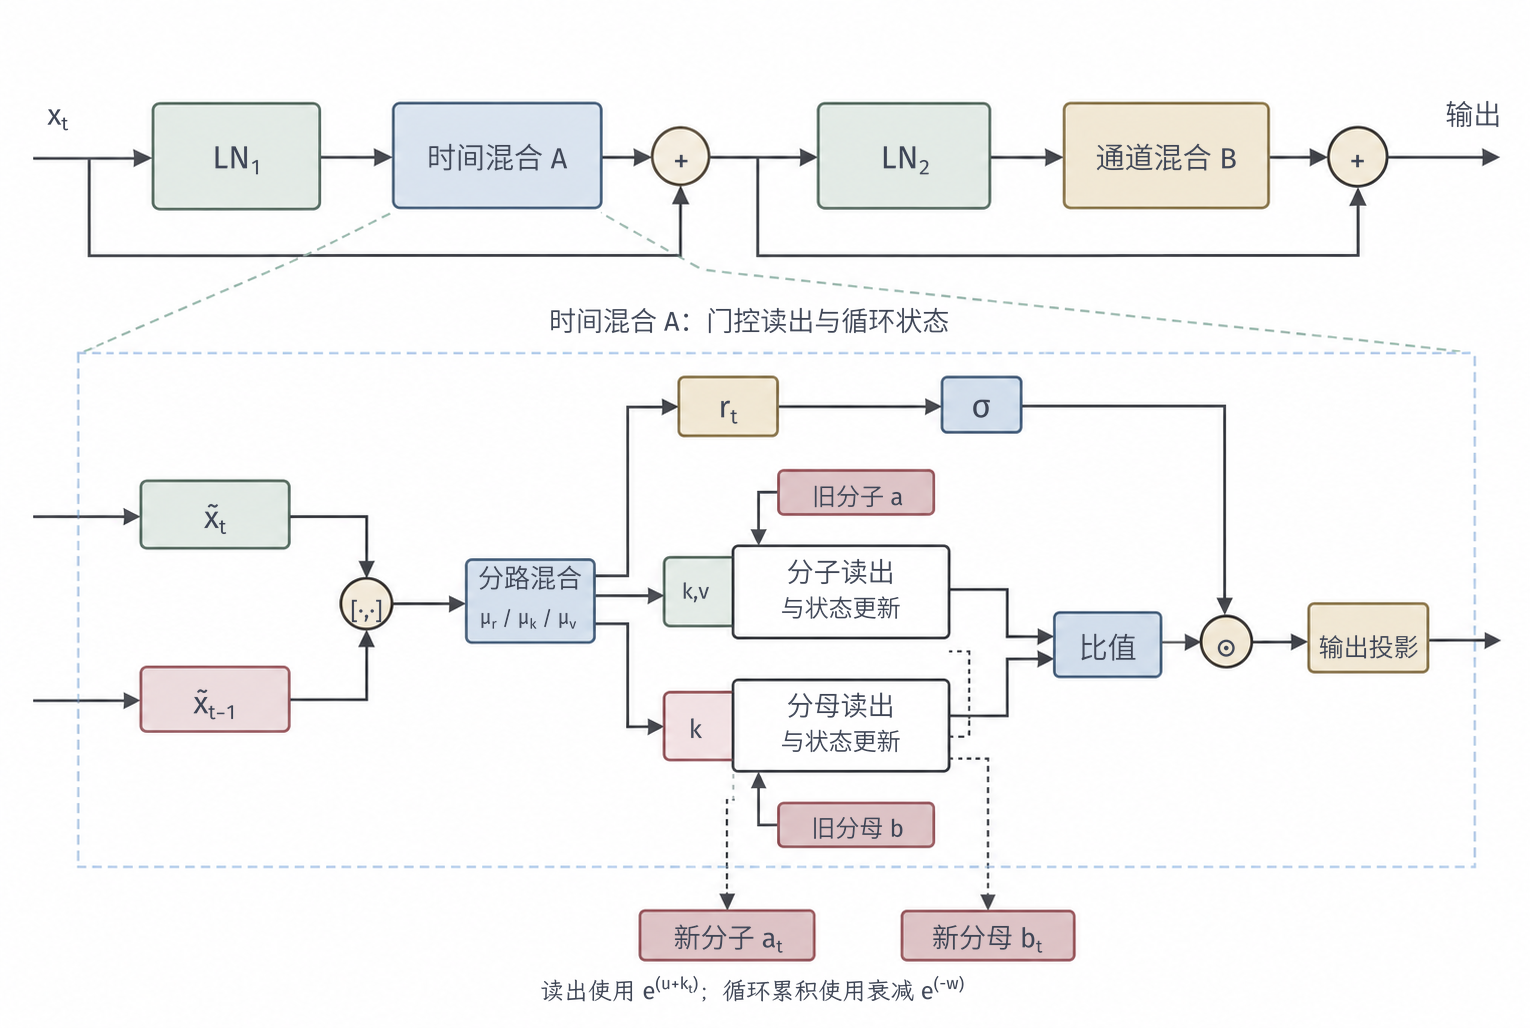
\includegraphics[width=129.540mm]{figures/05-neural-network-models/00-shared/generated/rnn-rwkv/figure.png}
  \caption{RWKV-4的完整残差层与时间混合子模块。上方在A、B之前分别归一化，并在各子模块之后作残差相加，第一次相加得到$\bm s_t$。下方只展开A，无箭头虚线表示对应关系；$\widetilde{\bm x}_t=\operatorname{LN}_1(\bm x_t)$是归一化后的特征。左下圆圈将当前与前一步的归一化输入打包为有序对，不把它们相加；分路混合分别采用$\bm\mu_r$、$\bm\mu_k$、$\bm\mu_v$，再形成各自的投影。下方展开分子、分母状态与读出之间的关系：循环更新使用$e^{-\bm w}$衰减，读出中另含当前键的$e^{\bm u+\bm k_t}$权重；精确递推见正文公式。图中省略稳定化重缩放、移位缓存的保存箭头及B的内部计算。}
  \label{fig:rnn-rwkv}
\end{figure*}
\FloatBarrier

沿图中的路径处理一个新词元时，先由A把历史累积与当前特征结合，产生对层输入的修正；第一次残差相加后，B再组合这一表示中的特征，产生第二次修正。因此，A的输出并不是下一词元的概率，完整层的输出也还需要后续层与词表读出。图中的两个子模块依次工作，却各自保留前一步的输入：A缓存的是上一位置进入时间混合的归一化表示，B缓存的是上一位置经过第一次残差相加后再归一化的表示。若把两份缓存混用，就改变了各自混合的对象。

逐词生成时，每一层都延续自己的累积状态和两份输入缓存。新词元从底层向上经过各层后，这些状态更新到同一个时间步，下一个词元便从此继续；不必重新处理已经读过的整个前缀。开始一条独立序列时，则需要重新初始化这些状态，避免上一条序列的信息进入当前预测。生成过程中，各层状态和门的取值随输入变化，用于计算它们的模型参数保持不变。

训练时，各位置的稠密投影可以批量计算，WKV核心仍处理有序累积；可使用顺序扫描，满足组合条件时也可采用并行前缀计算。投影、混合系数、衰减及门由任务损失共同更新。逐步预测则只延续累积、移位与数值尺度状态。按$d$个通道计，累积核心整段为$O(Td)$、持久状态为$O(d)$，稠密投影另有每步$O(d^2)$或$O(dd_{\mathrm{ff}})$成本；层数、词表与训练反向信息需另外计算。

\subsubsection{归一化权重与长期依赖}
\label{sec:rnn-rwkv-long-memory}

RWKV没有在累积状态上反复施加普通RNN的稠密非线性变换，旧贡献沿各通道按$e^{-w_i}$保留。较小的$w_i$提供较长时间尺度，较大的值强调近期；内容键再改变各位置写入的权重。对固定键与衰减，某个历史值坐标对当前聚合的直接系数是归一化权重：
\begin{equation}
  \frac{\partial v_{\mathrm{agg},j}^{(t)}}{\partial v_{i,j}}
     =\frac{\exp(-(t-1-i)w_j+k_{i,j})}
       {b_j^{(t-1)}+\exp(u_j+k_{t,j})},\qquad i<t\text{。}
  \label{eq:rnn-rwkv-value-gradient}
\end{equation}
它取决于内容与时间距离，不是一个任意非线性状态Jacobian矩阵的连乘。完整任务梯度还包含接收门、输出投影以及键变化的路径，并受归一化权重的尺度影响。

归一化约束了加权聚合的范围，却不取消遗忘。先单看历史贡献的未归一化权重。若$w_j>0$，早期权重仍会随距离指数减弱；实际读出的归一化系数还要除以当前分母，不能仅由这个衰减因子确定。即使$w_j=0$、所有键相同且当前偏置为零，单个位置的权重也会随位置数按$1/t$稀释。较大内容权重可以让某些位置更突出，但并未建立对每个历史位置重新执行查询的机制。

压缩还会合并不同历史。例如只看一个$w=0$、全部键为零的累积核心，值序列$(1,0,0)$与$(0,1,0)$都产生分子1、分母3。它们的位置不同，两个累积量却相同；只依据这组状态无法区分证据曾出现在哪一步。多通道、移位和深层非线性增加了可用表示，但仍需依据具体任务检查压缩后的可区分性。

RWKV因此用内容加权、可学习衰减和接收门组织可延续的历史，使训练投影便于批量计算、预测状态保持定长。它缓解了一部分普通非线性循环路径的困难，保留范围与检索能力仍由时间尺度、写入权重、层间计算和任务监督共同决定。

表~\ref{tab:rnn-state-models}统一比较上述状态模块。HiPPO是一套状态构造原则，S4、Mamba和RWKV是利用特定结构组织序列计算的网络设计，比较时分别记录状态构造原则、实际网络更新与计算组织，便于看出它们的组合关系。

\begin{table*}[htb]
  \small
  \begin{tabularx}{\linewidth}{@{}p{19mm}XXX@{}}
    \toprule
    模型或原则 & 历史表示与选择 & 整段计算 & 逐步持久状态 \\
    \midrule
    普通RNN & 非线性隐藏状态；全部坐标经共同更新 & 时间递推与BPTT & 单层$m$维状态 \\
    LSTM／GRU & 门调节保留和写入；LSTM另有记忆状态 & 通常逐步递推 & 等宽LSTM为$2m$，GRU为$m$ \\
    HiPPO & 基函数系数；测度与阶数决定近似范围 & 取决于所选更新与离散化 & $m$个投影系数 \\
    S4 & 结构化线性状态；固定时间响应 & LTI模块可用结构核与FFT卷积 & 每通道$m$维状态 \\
    Mamba & 输入相关步长、写入与读出 & 选择性仿射扫描 & $d$通道共$dm$维状态，另有短卷积缓存 \\
    RWKV-4 & 内容加权累积、时间衰减与接收门 & 批量投影和加权扫描等 & 两组累积向量及移位、数值尺度缓存 \\
    \bottomrule
  \end{tabularx}
  \caption{历史压缩与计算方式的比较。这里$m$表示状态宽度，$d$表示通道数，均按单层比较；持久状态只计流式预测中需延续的信息，不含参数、输出缓存和反向传播激活。稠密投影、层数与数值实现会改变完整网络的计算和存储。}
  \label{tab:rnn-state-models}
\end{table*}
\FloatBarrier

定长状态的代价不随已读长度线性增加，但相同宽度并不意味着相同的信息容量。循环注意力保存各位置编码状态，付出随输入长度增长的存储与读取；压缩状态把这一要求转为历史如何概括。两类模型的取舍应结合任务所需的精确位置访问、预测延迟和输入范围判断。

\FloatBarrier
\section{循环神经网络的扩展}
\label{sec:rnn-extensions}

此前的模型都沿一条单一的时间链组织状态：每个位置只看它前面的那一个位置。实际任务会在两个方向上突破这条链。其一是\emph{拓扑}：信息也许需要同时看到后文（双向）、沿图像的多个空间方向流动（多维），或按语法树那样的层次结构组合（树递归）——拓扑决定了一个状态在计算时能看到哪些对象。其二是\emph{深度}：同一位置的表示也可以像前馈网络那样纵向堆叠多层，让较低层形成局部特征、较高层在同一时刻做更抽象的组合——深度决定同一位置经历多少次表示变换。

\subsection{支持不同的拓扑结构}
\label{sec:rnn-topologies}

\subsubsection{双向循环与信息可见范围}
\label{sec:rnn-bidirectional}

许多离线序列任务（如给已经写好的句子逐词标注词性）在做某个位置的判断时，\emph{后文也是合法可见的}。而单向状态$\bm h^{(t)}$按定义只读取$\bm x_1,\ldots,\bm x_t$，天然看不到右侧。\term{双向循环网络}（bidirectional RNN）的做法很直接：用两套参数独立的循环网络，一套从左向右、一套从右向左读取同一序列，再在每个位置把两个方向的状态拼成该位置的表示：
\begin{equation}
  \begin{aligned}
    \overrightarrow{\bm{h}}^{(t)}&=F_{\rightarrow}\!\left(
       \overrightarrow{\bm{h}}^{(t-1)},\bm{x}_t\right),\\
    \overleftarrow{\bm{h}}^{(t)}&=F_{\leftarrow}\!\left(
       \overleftarrow{\bm{h}}^{(t+1)},\bm{x}_t\right),\\
    \bm{h}_t&=[\overrightarrow{\bm{h}}^{(t)};
                 \overleftarrow{\bm{h}}^{(t)}]\text{。}
  \end{aligned}
  \label{eq:rnn-bidirectional}
\end{equation}
两向通常使用不同参数，分别从序列两端的初态开始。反向上标$(t)$仍对齐输入位置，计算次序却是$T,T-1,\ldots,1$。两条链在同一步不必互相反馈，组合后的表示交给读出或下一层。

双向表示能使用后文，前提是后文在预测时已经可见。实时下一步预测若把尚未到达的观测送入反向链，就泄漏了未来信息；整段编码器用于转换任务则可以合法读取完整源序列。预测时已知哪些输入，决定了当前状态可采用哪一条信息路径。

\subsubsection{多维与多方向循环}
\label{sec:rnn-multidimensional}

规则网格中的当前位置可以依赖多个已计算的邻居。\term{多维循环网络}（multi-dimensional RNN）沿网格上的有向顺序组合这些前驱状态。例如二维网格的一个方向可采用
\begin{equation}
  \bm{h}_{i,j}=\tanh\!\left(
     \bm{U}\bm{x}_{i,j}+\bm{W}_1\bm{h}_{i-1,j}
      +\bm{W}_2\bm{h}_{i,j-1}+\bm{b}\right)\text{。}
  \label{eq:rnn-multidimensional}
\end{equation}
网格边界上的缺失前驱按约定初始化。该方向只读取上方和左方已形成的表示；按$i+j$分组时，同一对角线的节点可并行，而后续对角线依赖此前结果。再以其他角落为起点建立多个方向，就能组合不同象限的上下文\scite{graves2007mdrnn}

这里的多方向不是对同一条序列多跑几次，而是改变前驱关系。梯度沿多个前驱分支回传，对共享参数累积所有位置的贡献。直接把多路记忆相加还会增加状态幅度，门控、归一化和组合规则需随前驱数量设计；稳定性也要按新增前驱和完整组合规则分析。

\subsubsection{树递归与Tree-LSTM}
\label{sec:rnn-tree}

当输入本身带有语法树或层次结构时，强行按词的线性先后顺序组合未必合理：一个词最该先与谁结合，由句法关系而非相邻位置决定。\term{树递归网络}（recursive neural network）改为按树的父子依赖自底向上组合状态：先算出所有子节点的表示，再在父节点把它们合成更大子结构的表示，直到根节点得到整句表示。名称中的recursive描述的是\emph{结构上的递归}，与沿时间重复更新的recurrent不是一回事；本章把二者都放在“隐状态按某种依赖递推”的统一框架下比较。

二叉树可以把左右子状态拼接后变换；子节点数不固定时，可以先求和聚合。\term{树结构长短期记忆}（Tree-LSTM）为每个子节点设置遗忘门，以不同权重组合其记忆。以Child-Sum版本为例，令$C(j)$是节点$j$的子节点索引集合，$\bm{x}_j$是本节点输入，$\bm{h}_j,\bm{c}_j$分别为隐藏和记忆状态，计算
\begin{equation}
  \begin{aligned}
    \overline{\bm{h}}_j&=\sum_{k\in C(j)}\bm{h}_k,\\
    \bm{i}_j&=\operatorname{sigmoid}\!\left(
       \bm{U}_{\mathrm{i}}\bm{x}_j+\bm{W}_{\mathrm{i}}\overline{\bm{h}}_j
       +\bm{b}_{\mathrm{i}}\right),\\
    \bm{o}_j&=\operatorname{sigmoid}\!\left(
       \bm{U}_{\mathrm{o}}\bm{x}_j+\bm{W}_{\mathrm{o}}\overline{\bm{h}}_j
       +\bm{b}_{\mathrm{o}}\right),\\
    \widetilde{\bm{c}}_j&=\tanh\!\left(
       \bm{U}_{\mathrm{c}}\bm{x}_j+\bm{W}_{\mathrm{c}}\overline{\bm{h}}_j
       +\bm{b}_{\mathrm{c}}\right),\\
    \bm{f}_{j,k}&=\operatorname{sigmoid}\!\left(
       \bm{U}_{\mathrm{f}}\bm{x}_j+\bm{W}_{\mathrm{f}}\bm{h}_k
       +\bm{b}_{\mathrm{f}}\right),\qquad k\in C(j),\\
    \bm{c}_j&=\bm{i}_j\odot\widetilde{\bm{c}}_j
        +\sum_{k\in C(j)}\bm{f}_{j,k}\odot\bm{c}_k,\\
    \bm{h}_j&=\bm{o}_j\odot\tanh(\bm{c}_j)\text{。}
  \end{aligned}
  \label{eq:rnn-tree-lstm}
\end{equation}
叶节点的空和为零，参数形状与等宽链式LSTM相同。求和对孩子的重编号不变，但会弱化孩子次序；若左右位置具有不同语义，采用带位置参数的有序树版本更合适。Tree-LSTM的代表工作分别讨论了这两类结构\scite{tai2015}

图~\ref{fig:rnn-topologies}将依赖范围与计算顺序并列展示。树上的反向传播从父节点回到各孩子，多个损失的贡献在同一节点汇合；共享组合参数的梯度再对所有节点累积。两个叶子经树组合到共同祖先的路径可以短于按词序遍历的路径，但这种优势依赖给定树是否符合任务，还增加了结构取得与处理的要求。

\begin{figure*}[t]
  \centering
  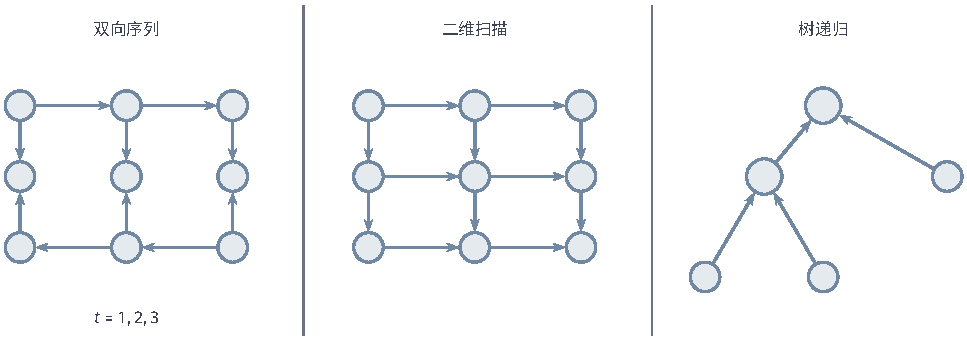
\includegraphics[width=163.791mm]{figures/05-neural-network-models/00-shared/tikz/rnn-topologies/figure.pdf}
  \caption{状态依赖拓扑。左图在同一输入位置组合正向与反向状态；中图由上方、左方前驱形成二维状态，箭头给出一个扫描方向；右图由叶节点向父节点组合子结构。圆节点表示各位置或子结构的状态，箭头表示状态依赖的方向。不同方向、位置或孩子组合是否共享参数，需要由具体模型说明。}
  \label{fig:rnn-topologies}
\end{figure*}
\FloatBarrier

例如，沿中图的箭头计算网格位置$(2,2)$时，直接使用的是$(1,2)$和$(2,1)$的状态。它们已经带来左上区域的信息，却尚未包含右侧$(2,3)$或下方$(3,2)$的输入。若任务需要这些区域的证据，就要增加从其他角落出发的方向，并在同一位置组合各方向的结果。左图的双向链采用同样的思路，让当前位置分别取得前文与后文的表示。

右图则改变了组合单位：两个叶子先在共同父节点形成局部子结构的表示，再与另一支的表示组合到根节点。这样，词语间的信息先后经过哪些状态，由给定树决定。选择拓扑时，首先要明确一次预测允许使用哪些输入，以及哪些输入应先组合；随后才能确定箭头、计算顺序和状态的含义。

\subsection{支持更深的网络}
\label{sec:rnn-depth}

时间展开的深度由序列长度决定，同一位置的表示变换深度则由层数决定。增加层数既可以让任务学习更多表示变换，也可以仅堆叠固定动态、提供更多历史特征。二者共享层次结构，却训练不同参数。

\subsubsection{堆叠循环网络：学习各层表示与时间动态}
\label{sec:rnn-stacked-networks}

\term{堆叠循环网络}（stacked RNN）让上层读取下层在相同位置的状态，同时维护自己的历史。设层数为$L$，$\bm h_0^{(t)}=\bm x_t$，则
\begin{equation}
  \bm h_{\ell}^{(t)}=F_{\ell}\!\left(\bm h_{\ell}^{(t-1)},
       \bm h_{\ell-1}^{(t)}\right),\qquad\ell=1,\ldots,L\text{。}
  \label{eq:rnn-stacked}
\end{equation}
上标是时间步，下标$\ell$是层索引。同一层跨步共享参数，不同层通常各用一组参数。单元可选普通RNN、LSTM或GRU；使用LSTM时，各层还维护自己的记忆状态$\bm c_\ell^{(t)}$。

第$t$步先计算底层，再把底层当前表示送到第二层，依次形成顶层表示。因而第二层同时读取“这一位置的底层特征”与“第二层此前形成的历史”。单向堆叠仍只使用当前及此前输入。

图~\ref{fig:rnn-stacked-network}展示三层网络的时间展开。水平箭头传递同层历史，垂直箭头传递同一时刻的层间表示。
\begin{figure}[htbp]
\centering
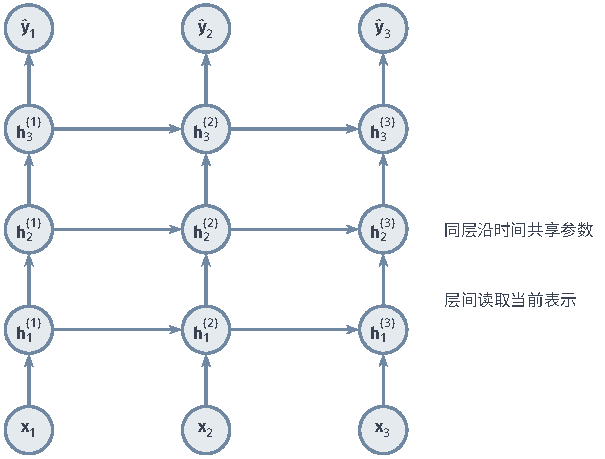
\includegraphics[width=102.369mm]{figures/05-neural-network-models/00-shared/tikz/rnn-stacked-network/figure.pdf}
\caption{三层堆叠循环网络。每层具有自己的循环参数并沿时间共享；上层读取下层当前状态与自身上一时刻状态，输出由顶层状态形成。图省略初态和层内门控。}
\label{fig:rnn-stacked-network}
\end{figure}
\FloatBarrier


以图中的第二个时间步为例，此时已保存三层在第一步的状态。输入$\bm x_2$先与$\bm h_1^{(1)}$形成$\bm h_1^{(2)}$，再由$\bm h_1^{(2)}$与$\bm h_2^{(1)}$形成$\bm h_2^{(2)}$，最后得到第三层的$\bm h_3^{(2)}$。这一次从底层到顶层的计算就完成了第二步；此前的输入$\bm x_1$通过各层保存的状态参与计算，无需重新输入。若单元采用LSTM，则每层还要同时更新并保存自己的$\bm c_\ell^{(2)}$。流式预测因此需要保存所有层的状态，单独保存顶层状态不足以继续下一步递推。

任务损失通常从顶层读出，也可以拼接或加权读取多个层。训练时梯度既沿时间回传，也沿层间依赖回传，各层循环与输入映射都接受任务监督。下层可以形成较局部的表示，上层再组合这些表示，但各层的时间尺度由实际动态和输入驱动决定，可以通过状态响应或任务行为检验。

若第$\ell$层宽度为$m_\ell$、$m_0=d$，普通稠密单元的整段计算量级为
\begin{equation}
  O\!\left(T\sum_{\ell=1}^{L}m_\ell(m_{\ell-1}+m_\ell)\right)\text{，}
  \label{eq:rnn-stacked-cost}
\end{equation}
门控单元还增加相应常数。完整反向计算需保存或重算各层各步的激活。层宽、读出范围与训练存储因此都影响深度选择。

\subsubsection{深度储备池计算：堆叠固定动态、学习统一读出}
\label{sec:rnn-deep-reservoir}

\term{深度储备池计算}（deep reservoir computing）把多个通常固定的储备池按层连接，利用层层动态形成历史特征，再训练任务读出。深度ESN是代表形式，第一层读取外部输入，上层读取下层当前状态\scite{gallicchio2018deepesn}

对泄漏积分单元，可写为
\begin{equation}
  \begin{aligned}
    \bm h_\ell^{(t)}&=(1-\alpha_\ell)\bm h_\ell^{(t-1)}
      +\alpha_\ell\tanh\!\left(\bm W_\ell\bm h_\ell^{(t-1)}
               +\bm U_\ell\bm h_{\ell-1}^{(t)}+\bm b_\ell\right),\\
    \widehat{\bm y}_t&=g\!\left(\bm V
       [1;\bm x_t;\bm h_1^{(t)};\ldots;\bm h_L^{(t)}]\right)\text{。}
  \end{aligned}
  \label{eq:rnn-deep-esn}
\end{equation}
$0<\alpha_\ell\leq1$是各层泄漏率，$\bm W_\ell,\bm U_\ell,\bm b_\ell$按构造固定，$\bm V$是可训练读出矩阵；也可以只读部分层。训练先逐步收集拼接特征，再拟合读出，平方损失时仍是一组扩展特征上的岭回归，不需要为固定循环参数执行任务梯度更新。

层叠改变输入经过的动态过滤。在线性标量简化且循环矩阵为零时，$h^{(t)}=(1-\alpha)h^{(t-1)}+\alpha u_t$，记忆按$(1-\alpha)^k$衰减，对$0<\alpha<1$的时间尺度为$-1/\log(1-\alpha)$。这说明不同泄漏率可以提供不同更新速度；真实储备池还包含反馈矩阵、输入驱动与非线性，整个模型的时间响应由这些因素共同形成。

各层也要检查回声状态性质。设相同输入下的两条轨迹距离为$\delta_\ell^{(t)}$，Tanh的Lipschitz性质给出
\begin{equation}
  \delta_\ell^{(t)}\leq r_\ell\delta_\ell^{(t-1)}
       +\alpha_\ell\lVert\bm U_\ell\rVert_2\delta_{\ell-1}^{(t)},
  \quad r_\ell=1-\alpha_\ell+\alpha_\ell\lVert\bm W_\ell\rVert_2\text{。}
  \label{eq:rnn-deep-esn-contraction}
\end{equation}
外部输入相同时$\delta_0^{(t)}=0$。

为看清下层差异怎样影响上层，令$\kappa_\ell=\alpha_\ell\lVert\bm U_\ell\rVert_2$，把式\eqref{eq:rnn-deep-esn-contraction}沿时间反复代入，得到
\[
 \delta_\ell^{(t)}
 \leq r_\ell^t\delta_\ell^{(0)}
   +\kappa_\ell\sum_{s=1}^{t}r_\ell^{t-s}\delta_{\ell-1}^{(s)}\text{。}
\]
右侧第一项只传播本层的初始差异，第二项累积下层在各步传来的差异。第一层接收的外部输入差始终为零，所以当$r_1<1$时，$\delta_1^{(t)}\leq r_1^t\delta_1^{(0)}\to0$。第二层及以上仍可能在每一步收到非零的下层差异，需要控制整个加权和。

设已经知道$\delta_{\ell-1}^{(s)}\to0$，且$0\leq r_\ell<1$。对任意$\varepsilon_0>0$，可以固定一个步数$M$，使$s>M$时$\delta_{\ell-1}^{(s)}\leq\varepsilon_0$。在$t>M$时，将驱动和拆成早期与晚期两部分：
\[
 \begin{aligned}
 \sum_{s=1}^{t}r_\ell^{t-s}\delta_{\ell-1}^{(s)}
 &=\sum_{s=1}^{M}r_\ell^{t-s}\delta_{\ell-1}^{(s)}\\
 &\quad+\sum_{s=M+1}^{t}r_\ell^{t-s}\delta_{\ell-1}^{(s)}\text{。}
 \end{aligned}
\]
早期部分只有固定的有限项，每项都随$t\to\infty$趋于零；晚期部分满足
\[
 \sum_{s=M+1}^{t}r_\ell^{t-s}\delta_{\ell-1}^{(s)}
 \leq\varepsilon_0\sum_{j=0}^{t-M-1}r_\ell^j
 \leq\frac{\varepsilon_0}{1-r_\ell}\text{。}
\]
乘上有界的$\kappa_\ell$后，晚期部分仍可随$\varepsilon_0$任意变小。本层初态项和早期部分又都趋于零，因而$\delta_\ell^{(t)}\to0$。从第一层开始，对有限个层依次使用这一步，就得到整个层叠的初态遗忘；这里使用的是下层差异趋于零，并没有假定上层的驱动在每一步都为零。

有限层数、各$r_\ell<1$且层间映射有界时，下层初态差异逐渐消失，上层受其驱动的差异也能衰减。这是充分条件；上述推导把各层收缩与层间有界映射共同计入，整个层叠的初态遗忘由这一组合条件支持。

与可训练堆叠RNN相比，深度储备池减少了循环动态的优化范围，多个层的特征可供同一读出选择；代价是固定状态变换不能按任务梯度重新安排记忆。层数、宽度、连接尺度和泄漏率通常由验证过程选择，测试数据不能参与这种选择。更多固定层可能增加有用时间特征，也可能增加冗余或压缩损失，需要与浅层储备池在相近预算下比较。

\subsubsection{跨层连接与分层读出}
\label{sec:rnn-depth-connections}

可训练网络与固定储备池都可以改变层间连接。维度相同时，跨层残差可写为$\bm u_\ell^{(t)}=\bm h_{\ell-1}^{(t)}+G_\ell^{(t)}$，其中$G_\ell^{(t)}$是这一层产生的变换结果；维度不同时先投影直达分支。残差为层方向提供较直接的梯度路径，通常没有缩短同一层的时间路径。

分层读出把不同层的状态送到任务头，使监督或读出可以直接使用多个层次的特征；它扩大了读出输入与参数规模。跨时间跳跃、跨层残差和门控可以组合；连接的起止状态与可训练参数确定各自的依赖路径。层深安排表示组合，时间尺度安排历史保留，读出范围安排任务访问。

\FloatBarrier
\section{理论分析}
\label{sec:rnn-theory}

与前两章一样，这里要把三个层面的问题严格分开，避免互相替代：\emph{表达能力}问定宽的隐状态是否\textbf{容纳}了预测所需的历史信息（两段不同历史若被映成同一状态，就再也无法区分）；\emph{收敛性}问BPTT能否把共享参数\textbf{优化}到梯度足够小的点；\emph{泛化性}问在有限条\emph{完整序列}上学到的规则，对新序列的\textbf{风险}有多大。状态递推是否稳定只是影响这些结论的一个条件，不能与“训练能否收敛”混为一谈。

\subsection{表达能力}
\label{sec:rnn-expressivity}

循环网络用固定宽度的状态概括任意长的历史，因此表达能力问题可以非常具体地表述为：\emph{这个定长状态，是否保留了区分不同历史所必需的信息}？一个判别准则是：如果两段不同的历史会把网络带到完全相同的状态，那么面对相同的后续输入和同一个读出，网络对它们给出的一切未来预测都必然相同。因此，凡是需要区分这两段历史的任务，网络在结构上就无法完成——与训练多久无关。计数、短期模式或有限状态机这类任务，往往可以用紧凑递推表达；而需要回忆任意久远细节的任务（如“在长序列开头看到的某个随机数是几”），则可能要求随序列增长的状态宽度、外部记忆或注意力式的直接读取。

门控改变哪些信息持续保存，堆叠改变每一步可组合的非线性变换。它们重组候选函数，却不保证任意长度目标都能在固定宽度和有限精度下实现。存储能力还受噪声、精度和连续性条件限制；无限精度实数状态与有限精度设备对应不同的可区分状态数。

\begin{theorem}[带前馈读出的循环网络对定长连续目标的逼近能力]
\label{thm:rnn-fixed-length-approximation}
固定长度$T$和每步输入维度$d$，输入序列取值于非空紧集$D\subset\mathbb R^{Td}$。允许宽度$2Td$的ReLU循环状态，以及末状态上的可变宽度前馈读出。对任意连续目标$g:D\to\mathbb R^q$和$\varepsilon>0$，存在该结构的候选$f$，使$\sup_{\bm x\in D}\lVert f(\bm x)-g(\bm x)\rVert_2<\varepsilon$。
\end{theorem}
\begin{proof}
每步以两组坐标保存$\rho(\bm x_t)$和$\rho(-\bm x_t)$，其余非负状态向后移动一个槽位，初态为零。固定移位矩阵与输入矩阵即可在第$T$步保存全部$T$个输入的正负部分。前馈读出从两部分之差恢复整段序列，再用定理~\ref{thm:ffn-continuous-approximation}逼近目标。
\end{proof}
这里的状态宽度随允许长度增长，读出也不是单个线性层。该结果证明定长序列的一类丰富循环候选可以逼近连续目标，没有保证固定窄状态能够处理任意长度。

有限精度给出另一条明确边界。若状态有$m$个坐标，每个坐标最多有$Q$个值，且后续只能读取这份状态，则最多能区分$Q^m$种历史。要在读取$T$个二值输入后，按随后给出的索引准确返回任意一个历史位，必须区分全部$2^T$种前缀，因而必须有$m\log_2Q\geq T$。否则两条不同前缀共用一个状态，查询它们不同的那一位时，至少有一个答案错误。无限精度的实数状态不受这个计数前提约束。

\subsection{收敛性}
\label{sec:rnn-convergence}

训练收敛描述参数更新过程，状态稳定性描述给定参数下的输入响应。Tanh使隐藏坐标有界，状态对参数的导数仍经过多步Jacobian矩阵乘积；持续变化的输入又可以使已训练模型的状态持续变化。

\begin{theorem}[循环网络完整BPTT的驻点收敛速度]
\label{thm:rnn-stationary-rate}
对固定训练集、有限长度序列和确定的初始化规则，完整BPTT给出训练目标$L(\bm{\theta})$的精确梯度。假设在包含迭代点及更新线段的区域内$L$可微、梯度为$\beta$-Lipschitz且$L\geq L_{\inf}$，其中$\beta>0$，采用固定步长$0<\eta\leq1/\beta$更新。下降引理给出
\begin{equation}
  L(\bm{\theta}^{(k+1)})
    \leq L(\bm{\theta}^{(k)})
       -\frac{\eta}{2}\lVert\nabla L(\bm{\theta}^{(k)})\rVert_2^2\text{，}
  \label{eq:rnn-descent}
\end{equation}
这里$(k)$是参数更新轮次，与状态时间步$(t)$分开。对任意$K\geq1$，将$K$次不等式相加得到
\begin{equation}
  \frac{1}{K}\sum_{k=0}^{K-1}
     \lVert\nabla L(\bm{\theta}^{(k)})\rVert_2^2
     \leq\frac{2\left(L(\bm{\theta}^{(0)})-L_{\inf}\right)}{\eta K}\text{。}
  \label{eq:rnn-stationarity}
\end{equation}
\end{theorem}
这个结论保证平均平方梯度随迭代次数变小，涉及趋近一阶驻点；该指标控制已计算迭代点的梯度尺度，全局最优与参数序列的极限还需其他条件。非光滑激活、随机梯度、裁剪或自适应优化改变了梯度或更新规则，其结论据相应条件另行建立。

循环结构会改变假设中的常数。状态对参数的一阶、二阶敏感度包含跨步传播，长序列与放大动态可能使允许的步长变小。较小梯度也可能来自早期路径消失，而不是目标已经满意；因此，梯度范数与训练误差需要同时解释。正交约束作用于线性部分，门控提供选择性路径，跳跃连接改变传播距离，但这些机制改变的是完整非凸目标中的部分传播条件。

截断BPTT还改变了梯度对象。将所用梯度写成$\widetilde{\bm{g}}=\nabla L+\bm{e}$，误差$\bm{e}$进入下降项$\langle\nabla L,\widetilde{\bm{g}}\rangle$，因而式\eqref{eq:rnn-descent}不再自动成立。若跨步状态Jacobian矩阵统一收缩且局部导数有界，被切断的远期贡献可由几何尾和控制；当长期保留的路径接近不衰减时，短截断就可能遗漏显著贡献。

这种遗漏不只是代价分析中的常数。若某参数只在首步读入证据时起作用，损失仅在很晚的末步出现，把中间状态断开后，该参数对当前片段损失的梯度可以为零，而完整梯度仍非零。前向状态可把证据带到末步，跨边界的反向路径才把末步损失传给形成证据表示的参数。

\begin{theorem}[储备池岭读出解的唯一性与线性收敛速度]
\label{thm:rnn-reservoir-readout-convergence}
固定储备池生成的设计矩阵$\bm Z$和标签矩阵$\bm Y$。式\eqref{eq:rnn-esn-ridge}采用$\lambda>0$并惩罚全部读出系数，则最小解唯一。记$\bm H=2(\bm Z^\top\bm Z+\lambda\bm I)$的最小、最大特征值为$\mu,L$。使用步长$1/L$的梯度下降时，
\[
 \lVert\bm R^{(K)}-\bm R^*\rVert_{\mathrm F}
 \leq(1-\mu/L)^K\lVert\bm R^{(0)}-\bm R^*\rVert_{\mathrm F}\text{。}
\]
\end{theorem}
$\bm H$正定保证唯一性；将读出误差更新写为$(\bm I-\bm H/L)$作用于每列，即得速度。这只覆盖固定状态特征的读出学习。端到端循环训练没有同样的凸性；连续目标在非空紧参数域上取得最小值，但最小值存在仍不保证BPTT能到达它。

\subsection{泛化性}
\label{sec:rnn-generalization}

讨论序列模型的泛化，首先要纠正一个极易犯的计数错误：\emph{一个长度为$T$的序列，是一个训练样本，而不是$T$个独立样本}。对独立评论分类，整段评论加一个标签才是一条样本；对多个独立设备的数据流，每条按约定长度切出的序列也算一条样本。序列内部各位置高度相关，若只是同一条长流上互相重叠的窗口，样本间更不独立，不能把它们当作独立同分布数据套用风险界，否则会严重高估有效样本量。下面的界中，$n$始终指\emph{独立完整序列}的条数。先用最朴素的有限候选情形看清泛化差距由什么决定。

\begin{theorem}[有限候选循环网络的期望风险界]
\label{thm:rnn-finite-risk}
设$\mathcal{F}$是限定结构、参数范围和输入长度后的预测函数族，$\bm{Z}_1,\ldots,\bm{Z}_n$为独立同分布的完整序列样本；$\bm{Z}$包含输入及相应目标。记有界损失为$\ell(f,\bm{Z})\in[0,1]$，风险为$R(f)=\mathbb{E}[\ell(f,\bm{Z})]$，经验风险为$\widehat R_n(f)=n^{-1}\sum_i\ell(f,\bm{Z}_i)$。设损失关于样本可测，$\delta\in(0,1)$。对预先固定的有限候选族，Hoeffding不等式与并合界给出，以至少$1-\delta$的概率，
\begin{equation}
  \sup_{f\in\mathcal{F}}\left|R(f)-\widehat R_n(f)\right|
    \leq\sqrt{\frac{\log(2|\mathcal{F}|/\delta)}{2n}}\text{。}
  \label{eq:rnn-finite-family-bound}
\end{equation}
\end{theorem}
统一界允许模型依据这些训练样本从候选中选择；$n$仍是独立序列数。无界交叉熵超出了这里的$[0,1]$条件；分析它时可另加预测概率下界、截断损失或尾部条件，并建立对应的风险界。

有限候选可以由预先固定的参数量化产生。

参数在有界区域内连续取值时，候选模型通常仍有无限多个，不能直接把全部模型逐个放入前面的有限候选并合界。我们可以在允许参数中预先选取有限个代表，让每个允许模型都由其中一个代表近似。近似会引入额外误差，因此要先控制参数改变怎样影响得分，再控制得分改变怎样影响损失。这两步都需要对所有允许输入统一成立，才能同时比较训练样本上的经验风险和新样本上的期望风险。

对连续参数，我们还可以把序列长度与循环权重的作用直接写入风险界。考虑零初态的单层循环网络
$\bm h_t=\sigma(\bm W\bm h_{t-1}+\bm U\bm x_t+\bm b)$、$f_{\bm\theta}(x)=\bm v^\top\bm h_T+c$，其中$\sigma$为1-Lipschitz且$\sigma(0)=0$。预先限制$\lVert\bm x_t\rVert_2\leq B_x$、$\lVert\bm W\rVert_2\leq r$、$\lVert\bm U\rVert_2\leq u$、$\lVert\bm b\rVert_2\leq b_0$、$\lVert\bm v\rVert_2\leq v_0$；所有参数展平为$\bm\theta\in\mathbb R^p$，其欧氏范数不超过$B_\theta$。令
\[
 G_T=\sum_{j=0}^{T-1}r^j,\qquad H_T=(uB_x+b_0)G_T\text{。}
\]
状态递推给出$\lVert\bm h_t\rVert_2\leq H_T$。

这个界适用于每个$1\leq t\leq T$：由零初态、$\sigma$的Lipschitz性质与$\sigma(0)=0$，每步都有$\lVert\bm h_t\rVert_2\leq r\lVert\bm h_{t-1}\rVert_2+uB_x+b_0$，展开后得到$(uB_x+b_0)\sum_{j=0}^{t-1}r^j\leq H_T$。将满足上述预先约束的参数集合记为$\Theta$，比较其中两组参数$\bm\theta$与$\widetilde{\bm\theta}$，并令$\Delta_\theta=\lVert\bm\theta-\widetilde{\bm\theta}\rVert_2$。因为$\Delta_\theta^2$是各参数块坐标差的平方和，每个向量块的差范数和每个矩阵块的Frobenius差范数都不超过$\Delta_\theta$；矩阵的谱范数又不超过Frobenius范数，所以也有$\lVert\bm W-\widetilde{\bm W}\rVert_2\leq\Delta_\theta$、$\lVert\bm U-\widetilde{\bm U}\rVert_2\leq\Delta_\theta$。

对同一条允许输入序列运行两组参数，记第$t$步状态差为$d_t=\lVert\bm h_t-\widetilde{\bm h}_t\rVert_2$。两条轨迹都从零开始，故$d_0=0$。在更新式中先只改变旧状态，再改变参数，得到
\[
 \begin{aligned}
 d_t\leq{}&r d_{t-1}
   +\lVert\bm W-\widetilde{\bm W}\rVert_2
       \lVert\widetilde{\bm h}_{t-1}\rVert_2\\
   &+\lVert\bm U-\widetilde{\bm U}\rVert_2 B_x
   +\lVert\bm b-\widetilde{\bm b}\rVert_2\\
 \leq{}&r d_{t-1}+(H_T+B_x+1)\Delta_\theta\text{。}
 \end{aligned}
\]
反复代入上式并使用$d_0=0$，各步参数差的贡献按几何系数相加，得到
\[
 \begin{aligned}
 d_t&\leq(H_T+B_x+1)\Delta_\theta\sum_{j=0}^{t-1}r^j,\\
 d_T&\leq(H_T+B_x+1)G_T\Delta_\theta\text{。}
 \end{aligned}
\]
读出还要计入$\bm v$与$c$的变化；把两组读出的差拆开，再使用同样的参数块界，有
\[
 \begin{aligned}
 |f_{\bm\theta}(x)-f_{\widetilde{\bm\theta}}(x)|
 &\leq v_0d_T\\
 &\quad+\lVert\bm v-\widetilde{\bm v}\rVert_2
       \lVert\widetilde{\bm h}_T\rVert_2
   +|c-\widetilde c|\\
 &\leq\bigl[v_0(H_T+B_x+1)G_T+H_T+1\bigr]\Delta_\theta\text{。}
 \end{aligned}
\]
这些上界只用了允许的长度、输入尺度和参数约束，没有随具体输入改变常数。

逐步比较两组参数，再比较读出，得到统一参数敏感度
\[
 |f_{\bm\theta}(x)-f_{\widetilde{\bm\theta}}(x)|
 \leq C_T\lVert\bm\theta-\widetilde{\bm\theta}\rVert_2,
 \quad C_T=v_0(H_T+B_x+1)G_T+H_T+1\text{。}
\]
每步状态差至多是前一步状态差的$r$倍，加上$(H_T+B_x+1)\lVert\bm\theta-\widetilde{\bm\theta}\rVert_2$；读出再加入权重与截距的差。这说明$C_T$从哪里来，而不是只把长度列为一个影响因素。

要让有限代表也能近似风险，还需把得分差转换为逐样本的损失差。沿用损失取值于$[0,1]$且关于样本可测的条件，并要求在每个允许目标下，损失关于得分都有同一个Lipschitz常数$L_\ell>0$。令$a_T=L_\ell C_T$，对任意完整序列样本$\bm Z$，就有
\[
 \begin{aligned}
 &|\ell(f_{\bm\theta},\bm Z)-\ell(f_{\widetilde{\bm\theta}},\bm Z)|\\
 &\quad\leq L_\ell|f_{\bm\theta}(x)-f_{\widetilde{\bm\theta}}(x)|\\
 &\quad\leq a_T\lVert\bm\theta-\widetilde{\bm\theta}\rVert_2\text{。}
 \end{aligned}
\]
对于预先固定的损失误差$\varepsilon>0$，取参数距离半径$\rho=\varepsilon/a_T$，便能保证相距不超过$\rho$的两个模型在任一样本上的损失差不超过$\varepsilon$。因此，下面按这个半径选出有限参数代表，再使用前面的有限候选风险界。


\begin{theorem}[有界参数循环网络在定长序列上的期望风险界]
\label{thm:rnn-continuous-risk}
在上述模型与预先固定的约束下，训练集含$n$个独立同分布的长度$T$序列。损失在$[0,1]$内、关于样本可测，且关于得分为$L_\ell$-Lipschitz，其中$L_\ell>0$。令$a_T=L_\ell C_T$，记期望风险为$R$、经验风险为$\widehat R_S$。对任意预先固定的$\varepsilon>0$和$\delta\in(0,1)$，以至少$1-\delta$的概率，任意训练输出$\widehat{\bm\theta}$满足
\[
 \begin{aligned}
 R(\widehat{\bm\theta})\leq{}&\widehat R_S(\widehat{\bm\theta})+2\varepsilon\\
 &+\sqrt{\frac{p\log(1+2B_\theta a_T/\varepsilon)+\log(2/\delta)}{2n}}\text{。}
 \end{aligned}
\]
\end{theorem}
\begin{proof}
参数域可由至多$(1+2B_\theta a_T/\varepsilon)^p$个半径$\varepsilon/a_T$的球覆盖，中心取自参数域。各中心使用Hoeffding不等式并作并合界；任意参数与最近中心的损失差不超过$\varepsilon$，在经验风险和期望风险中各贡献一项。

具体地，在固定参数域$\Theta$中选取尽可能多的点$\bm\theta_1,\ldots,\bm\theta_N$，使任意两点的距离大于$\rho$，且无法再加入满足这一距离要求的新点。以这些点为中心、半径为$\rho/2$的开球彼此不相交。每个中心的范数至多为$B_\theta$，所以这些小球全部包含在以原点为中心、半径为$B_\theta+\rho/2$的球内。$p$维球的体积与半径的$p$次方成正比，消去共同的单位球体积后得到
\[
 \begin{aligned}
 N(\rho/2)^p&\leq(B_\theta+\rho/2)^p,\\
 N&\leq(1+2B_\theta/\rho)^p\\
  &=(1+2B_\theta a_T/\varepsilon)^p\text{。}
 \end{aligned}
\]
这个体积界也保证上述选点过程只能得到有限个点。由于已经无法加入新点，任意$\bm\theta\in\Theta$到某个中心的距离都不超过$\rho$；否则可以把它加入。因此这些半径$\rho$的球覆盖$\Theta$，且中心仍满足模型的全部约束。参数域、$\varepsilon$、$\rho$及所选中心都在抽取训练样本之前固定。

对这些中心对应的$N$个模型，使用式\eqref{eq:rnn-finite-family-bound}中的Hoeffding并合界。令
\[
 \tau_{\mathrm{dev}}=\sqrt{\frac{\log(2N/\delta)}{2n}}\text{，}
\]
则以至少$1-\delta$的概率，所有中心同时满足$|R(\bm\theta_j)-\widehat R_S(\bm\theta_j)|\leq\tau_{\mathrm{dev}}$。在这一事件上，任取$\bm\theta\in\Theta$，选一个与它相距不超过$\rho$的中心$\bm\theta_j$。逐样本损失差不超过$\varepsilon$，所以取期望后有$|R(\bm\theta)-R(\bm\theta_j)|\leq\varepsilon$，对训练样本取平均后也有$|\widehat R_S(\bm\theta)-\widehat R_S(\bm\theta_j)|\leq\varepsilon$。于是
\[
 \begin{aligned}
 R(\bm\theta)
 &\leq R(\bm\theta_j)+\varepsilon\\
 &\leq\widehat R_S(\bm\theta_j)+\tau_{\mathrm{dev}}+\varepsilon\\
 &\leq\widehat R_S(\bm\theta)+\tau_{\mathrm{dev}}+2\varepsilon\text{。}
 \end{aligned}
\]
第一次近似把原模型的期望风险转到中心，第二次近似把中心的经验风险转回原模型；中间一步只使用所有中心共同成立的偏差界。由于这一事件内的链条对每个$\bm\theta\in\Theta$都成立，训练输出可以根据样本选择，也不必恰好等于某个中心。取$\bm\theta=\widehat{\bm\theta}$，再将$N$的体积上界代入$\tau_{\mathrm{dev}}$，就得到定理中的界。

\end{proof}
$r<1$时$G_T\leq1/(1-r)$，这组尺度条件下的敏感度可不随长度持续增大；$r=1$时该粗界至多按$T^2$增长，$r>1$时则可能快速增长。该结论展示了循环尺度怎样进入有限样本风险代价。门控、注意力或多层结构需要重新推导$a_T$，不能直接沿用这个单层常数。超过预先允许的长度、部署分布改变，或采用无界交叉熵时，都超出上述保证。

\FloatBarrier
\section{常见应用}
\label{sec:rnn-applications}

把循环模型用到具体任务时，真正决定成败的往往不是选了LSTM还是GRU，而是能否把四件事说清楚并在训练、预测两个阶段保持一致：\emph{可见输入}（做某个预测时哪些位置已经合法可见）、\emph{输出含义}（在哪个位置、输出什么量）、\emph{训练目标}（损失挂在哪些位置），以及\emph{状态的延续与重置}（什么时候沿同一序列接着算、什么时候必须清空）。下面用三类任务把这条完整流程串起来；具体的语言、信号和生成方法留给应用卷。

\subsection{序列分类}
\label{sec:rnn-application-classification}

以评论情感分类为例，一个样本是整段评论和类别$y$。沿用第~\ref{sec:rnn-encoder-decoder}节的嵌入查表方式，将离散词元映射为$\bm{x}_t=\bm{E}_{:,v_t}$，其中$\bm{E}\in\mathbb{R}^{d\times K_{\mathrm{vocab}}}$，$v_t$是词表索引，再用RNN、LSTM或GRU编码。末状态或掩码平均形成整段表示，经Softmax分类头输出概率，训练时对独立评论的交叉熵取平均；嵌入、循环单元和分类头共同更新。

单向编码适合边读边更新状态，但如果目标是整段类别，预测仍需说明何时决定结果。双向编码在读到完整评论后利用前后上下文；两向沿不同顺序读取，概括全段的状态分别位于正向有效末位置和反向有效首位置；也可以聚合各位置的双向表示。评估时保持分词、有效长度和聚合规则一致。

评论中的“并不精彩”提示模型需要组合否定与后续词，而不是只累计正向词频。这个例子指出了任务需要保留的关系，模型是否学得由预测结果检验。验证样本用于选择宽度、聚合和停止轮次，未参与选择的测试样本再用于评价。

\subsection{序列标注与时间预测}
\label{sec:rnn-application-aligned}

词语标注把每个有效位置的表示送入分类头，按照式\eqref{eq:rnn-aligned-loss}计算交叉熵。离线标注可用双向上下文，流式标注只使用当前已可见输入，或明确约定等待若干后续位置的延迟。循环状态提供输入历史的表示，逐位置Softmax分别预测各标签；若任务还要求标签组合合法，可以另接体现这些约束的输出模型。

以设备温度预测为例，$\bm{x}_t$可包含当前温度、控制量和已知时间间隔，读完这一步后输出下一时刻的温度估计$\widehat x_{t+1}$。有效预测位置集合记为$V$，平方目标为
\begin{equation}
  \ell=\frac{1}{|V|}\sum_{t\in V}
      (\widehat x_{t+1}-x_{t+1})^2\text{。}
  \label{eq:rnn-forecast-loss}
\end{equation}
目标位移必须在构造样本时完成，预测时不能输入待预测值。归一化统计只从训练数据估计，划分沿实际预测时间或按独立设备进行，避免重叠窗口把同一未来观测泄漏到训练与测试两侧。

流式使用时，传入新观测、更新状态、输出预测，再等待下一观测。跨片段可以延续同一设备状态，训练中则按截断长度切断梯度；设备切换、重新启动或大段缺失后的重置规则需要与训练匹配。多步预测若反馈自己生成的数值，误差可能累积；若使用未来外部变量，只能输入预测时确已知道的部分。历史用于形成已有信息下的预测，未来外部条件是否已知则决定了不同的预测任务。

\subsection{序列转换与生成}
\label{sec:rnn-application-generation}

转换任务给定源序列，生成另一段目标序列。训练流程是编码源输入，给解码器输入BOS和真实目标前缀，以包含EOS的目标计算式\eqref{eq:rnn-sequence-likelihood}，再联合更新全部模块。带注意力时，同时保留有效编码状态及掩码，供各解码步读取。

预测流程中，源编码只需执行一次。解码器从初始状态和BOS开始，输出一个条件分布，按约定策略选择符号，将该符号嵌入送入下一步；遇到EOS或预设最大长度停止。最大长度限制了计算和输出，EOS则是模型产生的结束符号。束搜索分别维护各候选前缀的解码状态，使后续更新对应各自的生成历史。

单序列生成也可采用\term{自回归模型}（autoregressive model）：按已有前缀预测下一个符号，再把生成结果反馈为后续输入。源条件可省略或由其他输入提供，循环更新、教师强制和停止条件仍需明确。每步贪心、束搜索和采样采用不同的输出策略，生成结果及其评价随策略而变；采样的多样性与预测分布的可靠性分别检验。

\FloatBarrier
\section{本章小结}
\label{sec:rnn-summary}

本章围绕一个共同机制展开——\emph{用一个随时间更新的隐状态，把变长历史中的有用信息带到当前}。可以沿五条主线收束。

第一，\textbf{基础递推与训练}。RNN用同一组参数在每个时间步更新状态、产生读出，因此能用固定参数处理任意长度；把时间链展开后用BPTT求导，梯度由共享参数在各时间步的贡献累加。展开后的深度随序列长度增长，这正是长序列训练困难的根源。

第二，\textbf{长期依赖的本质与三种解法}。早期信息要影响晚期输出，其梯度必须穿过状态Jacobian矩阵的多步连乘，持续小于$1$会梯度消失、持续大于$1$会梯度爆炸。由此自然分出三条改进路线：储备池\emph{固定}循环动态、只训练线性读出，回避长链求导；LSTM、GRU用可学习的门\emph{选择性}保留、写入和遗忘，并以加性记忆走廊让远期信息近无衰减速传递；注意力则绕开逐步链，\emph{保存各位置表示}并在需要时直达读取。

第三，\textbf{状态空间路线的统一视角}。线性状态更新同时是逐时刻递推、对历史核的因果卷积、以及可用关联扫描并行的前缀组合；HiPPO回答“状态该存什么历史”，S4用对角加低秩结构让长核高效稳定生成，Mamba让更新系数随输入内容选择，RWKV用内容加权和时间衰减维护定长累积状态。它们在“整段可并行训练”和“逐步只存定长状态”之间取得不同平衡。

第四，\textbf{拓扑与深度}。双向、多维、树递归改变信息可见的拓扑（双向读取要求后文在预测时已经可见，树递归要求给定结构）；堆叠循环网络在同一位置增加纵向表示深度。跨层或跨时间的近道能缩短梯度路径，却不能替代时间记忆本身。

第五，\textbf{三个理论层面互不替代}。定长状态是否保留了区分历史所需的信息（表达）、BPTT能否把梯度降到驻点（收敛）、以及在$n$条\emph{独立完整序列}上学到的规则风险有多大（泛化），各有条件：能执行更长的递推并不等于能推广到更长序列，结构、优化和样本假设必须分别检验。

\paragraph{扩展阅读}
Goodfellow等教材第10章系统讨论序列建模、时间展开与循环网络的训练，可结合本章的状态更新式和计算图阅读\scite{goodfellow2016}LSTM原论文见第\ref{sec:rnn-lstm}节，可进一步比较记忆状态的前向传递与误差的反向传播。

\chapter{图神经网络}
\label{chap:graph-networks}

先想一个看似简单的任务：预测一个分子是否有毒。分子由数量不一的原子通过化学键连接而成——有的分子含5个原子，有的含50个，一个碳原子可能连2个邻居也可能连4个。我们手里已有前几章的网络，却会发现它们都不好直接用：若把所有原子属性拼成一个固定长度向量喂给前馈网络，分子一大就装不下，而且\emph{只要给原子重新编号、调换拼接顺序，输入向量就变了}，可分子还是同一个分子；用卷积？图像里有整齐的网格和“左邻右舍”，分子没有；用循环网络逐个读原子？原子之间根本没有天然的先后顺序，强行规定一个遍历次序只会引入人为偏见，而且化学键连接的对象未必在序列中相邻。

这些例子的共同点是：数据的核心信息在于\emph{对象之间的关系}，而关系既不规则、也没有顺序。预测论文类别时，一篇论文的类别不仅取决于正文，还取决于它引用了谁、被谁引用；社交网络中一个人的行为与其朋友相关。若只把对象属性交给网络而不告诉它连接关系，等于丢弃了这类数据最关键的结构。于是本章要回答：\emph{网络怎样直接把“谁与谁相连”作为计算的组织依据，让数量可变、连接不规则的对象互相交换信息，同时保证给对象重新编号不会改变预测的含义}？

思路是让信息\emph{沿边流动}：每个节点反复地从与它相连的邻居那里收集信息、汇总后更新自己的表示；经过若干轮，一个节点的表示就浓缩了它周围一片子结构的信息，最后可用于预测节点、边或整张图。这立刻引出本章的几条主线：每个节点\emph{从哪些邻居读取}、如何把\emph{数量可变}的邻居组合成定长表示（一轮消息传递）；\emph{传播多少轮}决定关系影响能传多远；以及如何让这种计算\emph{对重编号不敏感}（置换对称）。随后还会看到，关系可能分类型、随时间变化、涉及多个对象或带几何坐标，这些都会约束消息的形式；最后仍要回到表达能力、优化与泛化，追问这些结构在什么条件下真的有用。

\section{图神经网络概述}
\label{sec:gnn-overview}

先用一个思想实验看清“不利用连接”会错在哪里。假设引用网络中有两篇内容特征完全相同的论文，但一篇引用了一系列高水平工作、另一篇只引用无关文献；只看论文自身描述向量的前馈网络会给它们相同预测，可它们的学术影响力显然可能不同。再看结构本身：卷积之所以能共享规则，靠的是网格上每个位置都有明确的“左上邻居”；但在一般关系网络里，节点的邻居既没有固定数量、也没有自然次序，更不存在一个能在全图滑动的固定窗口——编号之差（节点3和节点5）只反映存储位置，不代表任何“距离”。循环网络能读一串对象，却必须先人为指定遍历次序。图网络的根本不同在于：\emph{让输入中给定的连接关系，直接决定每个节点在计算时读取谁}。

把原子、论文等对象记为节点，把它们之间给定的关系记为边。输入图为$\mathcal G=(V,E)$，$V=\{1,\ldots,n\}$，$e=|E|$。
节点$i$的属性为$\bm x_i\in\mathbb R^d$，消息边$j\to i$的属性记为$\bm a_{i,j}\in\mathbb R^{d_e}$。
消息下标先写接收者，再写发送者，与有向边的起点、终点记法分别使用。
分子属性可包含原子与键类型，引用网络的属性可包含论文内容。图对象的其他表示、邻接矩阵的方向约定以及后文使用的图谱变换基础，可参考\BookChapterRef{chap:graph-theory}{卷1《数学准备：计算、分析与几何》的“图的表示与计算”章}。

若有向邻接矩阵以行记起点、列记终点，本章为直接写出接收端汇总，使用其转置
$\bm A=\bm A_{\mathrm{graph}}^\top$，因此$\bm A_{i,j}$为$j\to i$的权重。
$N(i)=\{j:\bm A_{i,j}\ne0\}$是发送有效消息的入邻域；
零权结构边若仍需参与计算，应另存结构掩码。无向图上矩阵对称，两种表示相同。
后文的谱域推导采用非负权重无向图，基础消息传递允许有向边。

\term{图神经网络}（graph neural network, GNN）让网络沿给定关系交换并组合对象的表示。它把“谁与谁相连”变成计算的组织依据，而所有节点共用同一套更新规则，因此同一个网络可以直接处理节点数不同、邻居数不同的图，而不必为每个节点、每种规模单独设置参数。这里的图用于组织输入对象之间的计算；边的含义由原始关系给定（引用、化学键等），模型本身并不自动声称这些关系代表因果或条件独立——那样的解释需要各自的建模依据。

\paragraph{为什么必须谈置换对称。}
图的节点编号只是存储用的标签：把分子里的碳原子从3号改叫7号，分子没有任何变化，预测也不该变。这给图网络施加了一条前几章没有的硬约束。令$\bm{X}\in\mathbb{R}^{n\times d}$按行存放节点特征，即$\bm{X}_{i,:}=\bm{x}_i^{\top}$；用\term{置换矩阵}（permutation matrix）$\bm{P}$重新排列这些行，则新的输入为$\bm{X}'=\bm{P}\bm{X}$、$\bm{A}'=\bm{P}\bm{A}\bm{P}^{\top}$，边属性也须同步重排（节点换号后，连在它身上的边必须一起换）。两种任务对应两种不同的对称要求：\term{置换等变性}（permutation equivariance）针对\emph{节点级}输出——节点跟着重排，每个节点的预测也必须跟着它一起重排，保证“原来那个原子的预测仍对应那个原子”；\term{置换不变性}（permutation invariance）针对\emph{整图}输出——分子的毒性等整体性质在原子重编号后必须保持不变。不含边属性时，两种要求可写为
\begin{equation}
  \begin{aligned}
    F(\bm{P}\bm{A}\bm{P}^{\top},\bm{P}\bm{X})
      &=\bm{P}F(\bm{A},\bm{X}),\\
    f(\bm{P}\bm{A}\bm{P}^{\top},\bm{P}\bm{X})
      &=f(\bm{A},\bm{X})\text{。}
  \end{aligned}
  \label{eq:gnn-permutation}
\end{equation}
$F$产生按节点排列的输出，$f$产生整图输出。重编号后，每个原子的预测仍对应同一个原子，分子的属性预测仍对应同一个分子；这里保持的是每个原子与其输出的对应，不同原子仍可有不同预测。

沿关系学习表示的思想早于今天的图卷积层。早期处理树和有向无环结构的递归网络，沿既定依赖逐步形成表示；一般图出现环时，邻居状态可能互相等待，需要给这一组依赖安排确定的求值方式。Gori等在2005年提出图神经网络模型，将节点状态定义为相互依赖方程的解，允许直接处理带环的图，并区分节点任务与整图任务\scite{gori2005graphdomains} Scarselli等在2009年的系统论述中，以共享局部更新和收缩条件保证状态解唯一，再通过反复更新求得稳定状态。共享更新把关系纳入表示，不动点求解处理环内依赖；所用收缩条件同时限定了更新函数的候选范围\scite{scarselli2009gnn}

另一条路线试图把卷积网络的共享滤波推广到不规则结构。Bruna等在2014年的Spectral CNN中，用图拉普拉斯的特征向量替代普通傅里叶模式，在这些模式上学习滤波响应。它给出了图卷积的谱域定义，但显式特征基带来计算成本和跨图使用的困难\scite{bruna2014spectral} Defferrard等在2016年以切比雪夫多项式实现谱滤波，使计算转为有限邻域上的稀疏传播，无需显式求出完整特征基。多项式把计算改为稀疏传播，并将能够读取的范围限定到相应的跳数\scite{defferrard2016chebnet}

到2016至2017年，图上的有限轮次计算形成了几种不同设计。门控图网络用门控状态更新替代必须迭代至不动点的求值方式；GCN把谱滤波的低阶近似改写为简单的归一化邻域层，便于用节点标签端到端训练；GraphSAGE通过采样与共享聚合，为大图和未见节点组织计算。它们分别重新安排状态求值、传播算子和邻域读取。后文据此说明每种模型改变的信息路径与执行代价。

比较这些设计，需要把消息产生、节点更新和任务输出放在同一计算框架中。Gilmer等在2017年把许多分子图模型概括为消息计算、状态更新和整图读出，使节点、边属性及参数共享的位置能够明确对照\scite{gilmer2017mpnn} 随后的问题从“能否沿边计算”转向“应保留哪些差别”：2018年的GAT用内容决定邻居权重，2019年的GIN联系邻域聚合与图结构区分能力。相关研究还将状态扩展到多种关系、随时间出现的事件及带几何坐标的对象，并分析传播过深时的信息损失。这些方向共同说明，图网络的发展既关心计算规模，也关心关系语义、对称性与表示能力。

消息传递、图卷积和循环更新可以出现在同一个模型中。基础结构回答如何沿边传递信息；卷积模型进一步规定传播算子；循环模型强调同一更新规则反复作用于状态。图的边可以形成环，但固定轮次展开后的计算图仍沿轮次前进，能够使用前面章节的反向传播。

\section{基础图神经网络}
\label{sec:gnn-basic}

本节先给出图网络最通用的计算框架——消息传递。设计它时要同时解决两个工程难题：其一，怎么把邻居的属性变成可以利用的信息；其二，更棘手的是\emph{不同节点的邻居数量不一样}（度从0到上百都可能），如何把任意数量的邻居映射成一个固定宽度的向量，供后续统一处理。一个自然的朴素想法是“把所有邻居特征按编号拼接”，但这会同时撞上两堵墙：输入宽度随最大度数变化、无法固定；而且拼接结果依赖邻居的枚举次序，给邻居重新编号就改变了输入，违背置换等变。正确做法是分两步——对每条边用\emph{同一个}共享的消息函数算出一条定长消息，再用一个\emph{与枚举次序无关}的操作（求和、平均、取最大）把任意多条消息聚合成一个定长向量。

\subsection{网络结构}
\label{sec:gnn-structure}

\term{消息传递}（message passing）可以概括为“收信—汇总—更新”三步：每个节点沿入边接收邻居发来的消息，把它们聚合成一个邻域摘要，再结合自己原有的表示更新状态。这里的“消息”就是一条边为后续计算提供的数值向量，不要与分布式系统中实际传输的数据包混淆——它只是对一次局部计算的称呼。用$\bm{h}_i^{(l)}\in\mathbb{R}^{m_l}$表示节点$i$在第$l$轮之后的隐表示，初态可取$\bm{h}_i^{(0)}=\phi_{\mathrm{in}}(\bm{x}_i)$。一轮计算由三个步骤组成：
\begin{equation}
  \begin{aligned}
    \bm{m}_{i\leftarrow j}^{(l)}
      &=M^{(l)}\!\left(\bm{h}_i^{(l)},\bm{h}_j^{(l)},\bm{a}_{i,j}\right),\\
    \overline{\bm{m}}_i^{(l)}
      &=\operatorname{AGG}^{(l)}
        \!\left(\{\!\{\bm{m}_{i\leftarrow j}^{(l)}:j\in N(i)\}\!\}\right),\\
    \bm{h}_i^{(l+1)}
      &=U^{(l)}\!\left(\bm{h}_i^{(l)},\overline{\bm{m}}_i^{(l)}\right)\text{。}
  \end{aligned}
  \label{eq:gnn-message-passing}
\end{equation}
$M^{(l)}$是消息函数，输出固定维度的消息；$\operatorname{AGG}^{(l)}$是聚合函数，把任意数量的消息组合成一个固定维度的向量；$U^{(l)}$是节点更新函数。理解聚合为什么要用双花括号记法很重要：它表示一个\term{多重集合}（multiset）——其中的元素\emph{没有顺序}（保证重编号不影响结果），但\emph{每个元素重复出现的次数仍然算数}。这一点区别于普通集合：两个邻居恰好具有相同状态时，求和会计入两次而非一次，邻居的数量本身就是信息（后面讲GIN时会看到，是否保留这种重复次数直接决定网络的表达能力）。

聚合通常选求和、平均或逐坐标最大值，也可以先计算权重再加权求和。空邻域上的求和取零；平均和最大值需要另约定空输入，例如取零并提供空邻域标记。另一种做法是加入\term{自环}（self-loop），使节点也向自身发送消息。自环是否与普通边共享参数由模型规定；更新若另读自身状态，还需说明两条自身路径怎样共同作用。

图~\ref{fig:gnn-message-passing}把节点$i$的一轮计算展开。各邻居先通过同一消息函数，再进入对次序不敏感的聚合；节点自己的旧表示另进入更新。这种分工既容纳边属性，也保留自身与邻居信息的区别。
\begin{figure*}[htb]
  \centering
  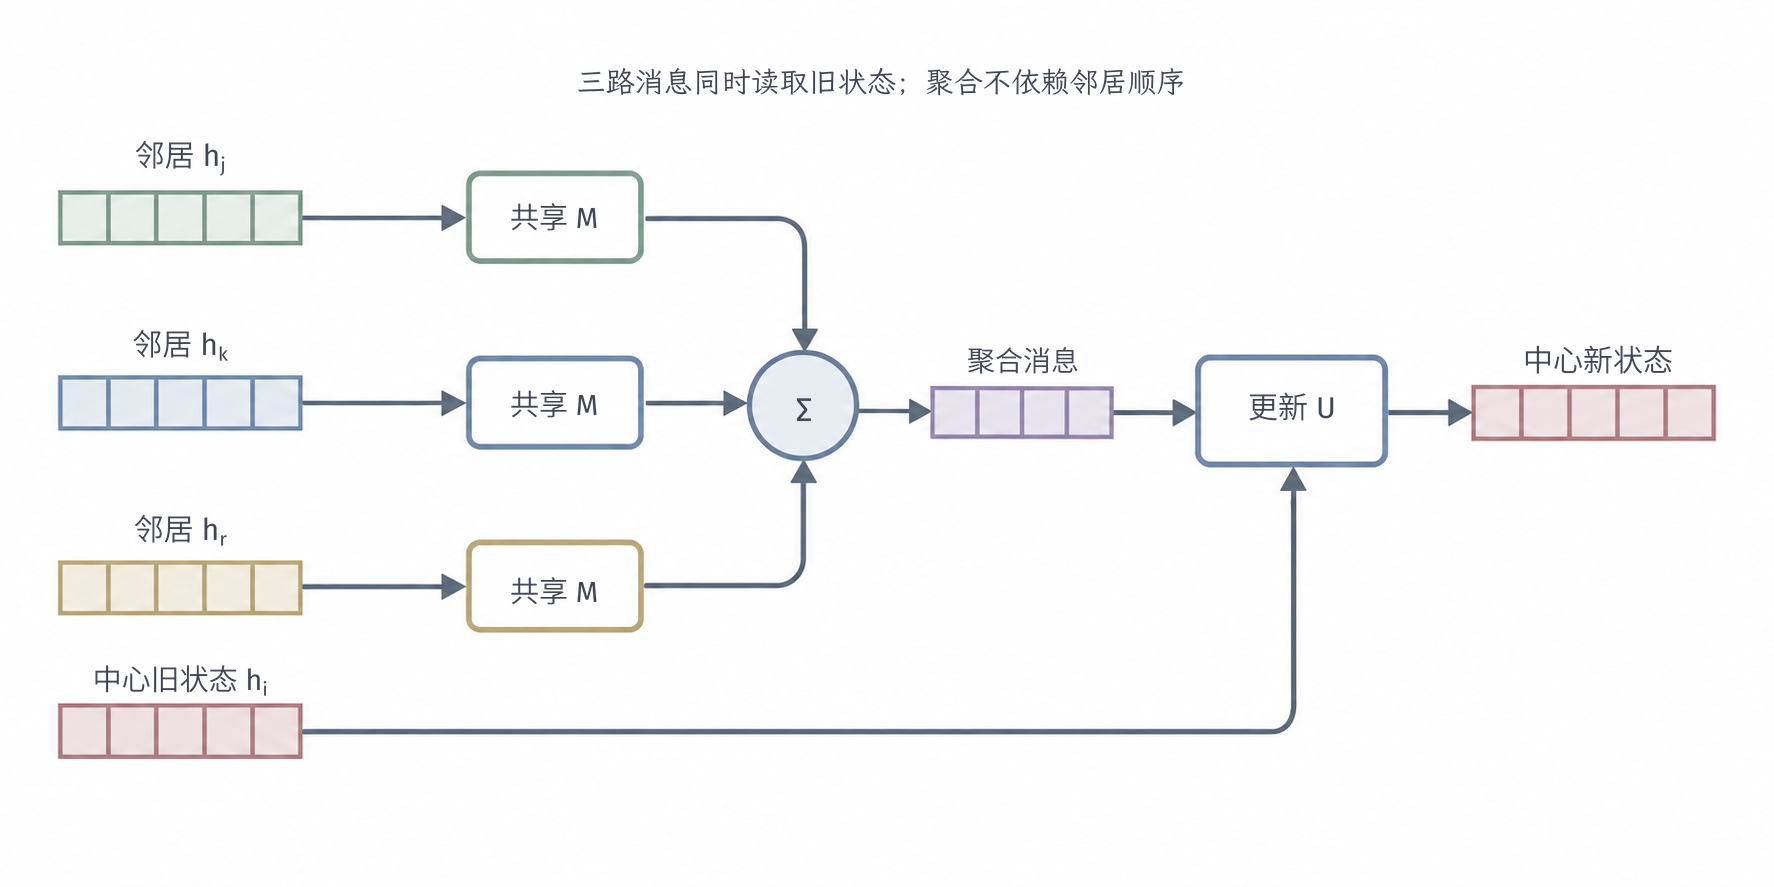
\includegraphics[width=150.199mm]{figures/05-neural-network-models/00-shared/generated/gnn-message-passing/figure.png}
  \caption{节点$i$的一轮消息传递。左侧三行邻居表示分别产生消息，经求和聚合后更新节点$i$。下方独立路径把$i$的旧表示送入更新函数。图中省略消息函数对接收节点和边属性的额外输入，所有节点使用相同的消息与更新规则。}
  \label{fig:gnn-message-passing}
\end{figure*}
\FloatBarrier

在同一轮内，$M^{(l)}$和$U^{(l)}$的参数在所有节点与边上共享。因此，增加节点会增加计算量，却不必增加参数量。若邻域聚合不依赖枚举次序，输入编码和节点更新也使用共享函数，就可按轮归纳证明式\eqref{eq:gnn-permutation}：重编号只重排消息的接收位置，聚合结果跟着重排，更新后的表示也跟着重排。随机邻居采样还要求采样规则与编号无关；不同随机抽样下输出数值未必一致，等变性应针对对应的抽样或输出分布理解。

一轮只能读取直接邻居的旧表示，这正像卷积网络中一层只覆盖一个局部窗口。要让信息传得更远，靠的是\emph{多轮传播}：两轮之后，每个邻居的表示里已经含有它自己邻居的信息，于是当前节点间接看到了两跳之外的节点。\term{图上的感受野}（graph receptive field）就是能够经传播影响当前表示的节点范围；在仅使用一跳邻域、没有全局通路时，$L$轮的范围至多为$L$跳。图~\ref{fig:gnn-propagation}采用同步更新：所有节点都先看上一轮的旧快照、各自算出新快照后再统一替换——这样可以避免“同一轮里先更新的节点被后更新的节点提前看到”，保证一轮最多只能获得一跳的新信息。若改为读取刚更新的状态，传播次序和每轮可见范围都会随之改变。

\begin{figure}[htb]
  \centering
  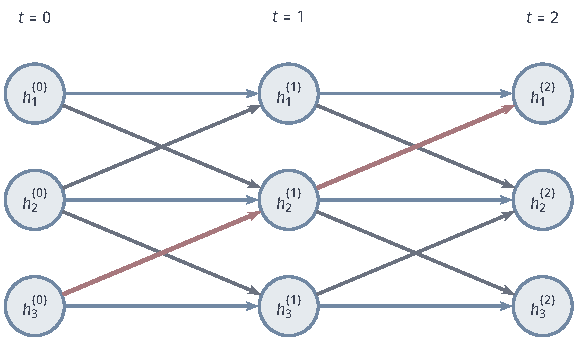
\includegraphics[width=97.794mm]{figures/05-neural-network-models/00-shared/tikz/gnn-propagation/figure.pdf}
  \caption{三节点路径上的同步传播。列顶的$t=0,1,2$表示同步快照，横向实线传递自身状态，斜线沿原图的相邻关系传递状态。红色粗线描出节点3经节点2影响节点1的两跳路径；同一列内没有即时传播，因此一次更新不能直接读取两跳之外的新信息。}
  \label{fig:gnn-propagation}
\end{figure}
\FloatBarrier

\begin{example}[两轮邻域平均]
\label{ex:gnn-two-rounds}
取无向路径$1-2-3$，初始标量为$\bm{x}=(1,0,2)^{\top}$。为单独观察传播，暂不使用可学习参数与非线性，令
\[
  h_i^{(l+1)}=\frac{h_i^{(l)}+\sum_{j\in N(i)}h_j^{(l)}}{1+|N(i)|}\text{。}
\]
一轮结果为$(1/2,1,1)^{\top}$，两轮结果为$(3/4,5/6,1)^{\top}$。节点1在第一轮没有读取节点3，第二轮却通过节点2受到节点3的影响。这是人为构造的传播例子，不是训练所得的实验结果。
\end{example}

节点表示形成后，整图预测还需要\term{读出}（readout）：把数量可变的节点表示变成一个图表示。基本形式是
\begin{equation}
  \bm{g}=\rho\!\left(\sum_{i\in V}\phi(\bm{h}_i^{(L)})\right),
  \qquad \widehat{\bm{y}}=g_{\mathrm{out}}(\bm{g})\text{，}
  \label{eq:gnn-readout}
\end{equation}
其中$\phi$是共享的节点变换，$\rho$是聚合后的变换。求和不因节点重排而改变，所以它把节点等变表示转为整图不变表示。平均会消去部分规模信息，最大值强调是否出现某类特征；若目标随对象数量累积，求和更符合这一结构假设，但仍需验证目标是否具有相应可加性。

只计固定宽度$m$下的稠密线性节点变换和线性消息，一轮常可组织为$O(nm^2+em)$：先对节点变换，再沿边聚合。若每条边都单独通过宽度为$m$的稠密网络，边计算可以达到$O(em^2)$。消息函数的形式和特征宽度共同决定边数的成本系数。保存多轮激活时，训练存储也随节点、边及传播轮次增长；参数共享控制的是参数数目。

\subsection{输出和学习目标}
\label{sec:gnn-output-objectives}

消息传递得到的是每个节点一个表示，但实际要预测的对象可能在三个不同层级：单个节点、一对节点（边）、或整张图。三者可以共用同一个图编码器，区别只在\emph{从哪里读出、用什么损失}。这一区分很重要，因为它决定了是否还能保留节点身份：节点/边任务要求输出与具体位置对应（置换等变），整图任务则必须把所有节点汇成一个与编号无关的量（置换不变）。图~\ref{fig:gnn-output-levels}把这三种读出对应起来；损失函数仍按第~\ref{sec:ffn-output-objectives}节介绍的输出含义选择。

\begin{figure*}[htb]
  \centering
  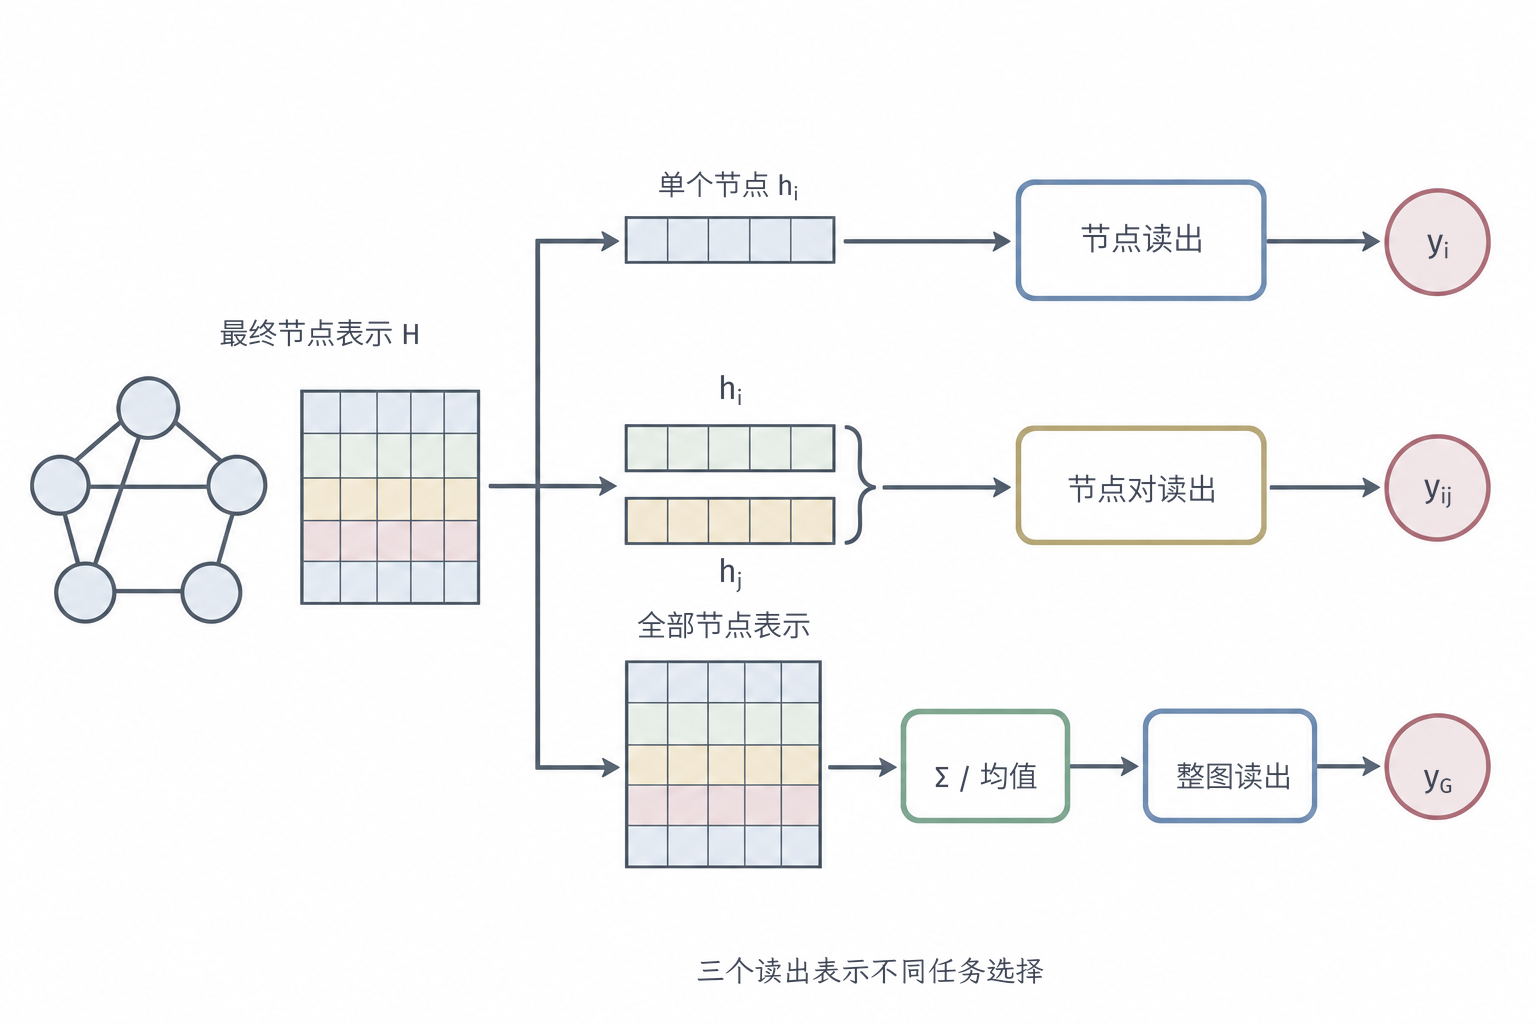
\includegraphics[width=130.048mm]{figures/05-neural-network-models/00-shared/generated/gnn-output-levels/figure.png}
  \caption{同一组节点表示的三种任务读出。三个分支分别承载节点、节点对和整图任务，并在相应位置执行读出。节点预测读取一个节点，边或连接预测读取两个端点及可用的关系属性，整图预测先对全部节点作对称聚合；三个分支不要求在同一模型中同时启用。}
  \label{fig:gnn-output-levels}
\end{figure*}
\FloatBarrier

节点分类在每个受监督节点上计算类别概率。设类别数为$C$，标签$y_i\in\{1,\ldots,C\}$，训练标签所在节点集合为$V_{\mathrm{train}}$，则
\begin{equation}
  \begin{aligned}
    \bm{p}_i&=\operatorname{softmax}(\bm{W}_{\mathrm{out}}\bm{h}_i^{(L)}+\bm{b}_{\mathrm{out}}),\\
    L_{\mathrm{node}}&=-\frac{1}{|V_{\mathrm{train}}|}
      \sum_{i\in V_{\mathrm{train}}}\log p_{i,y_i}\text{。}
  \end{aligned}
  \label{eq:gnn-node-loss}
\end{equation}
$\bm{W}_{\mathrm{out}}\in\mathbb{R}^{C\times m_L}$，$\bm{b}_{\mathrm{out}}\in\mathbb{R}^{C}$。其他节点的可见属性与连接可以按任务设定参加编码，类别标签则放在各自的监督或评估集合中。标签掩码限定哪些节点产生训练损失，输入特征的可见范围由另一个规则确定。

边预测需要同时读取端点。设候选节点对集合为$B$，用成对读出函数计算得分，再变成存在连接的预测概率：
\[
  \begin{aligned}
    s_{i,j}&=g_{\mathrm{pair}}(\bm{h}_i^{(L)},\bm{h}_j^{(L)},\bm{a}_{i,j}),\\
    p_{i,j}&=\operatorname{sigmoid}(s_{i,j})\text{。}
  \end{aligned}
\]
对二值目标$b_{i,j}$可使用
\begin{equation}
  L_{\mathrm{edge}}=-\frac{1}{|B|}\sum_{(i,j)\in B}
    \left[b_{i,j}\log p_{i,j}+(1-b_{i,j})\log(1-p_{i,j})\right]\text{。}
  \label{eq:gnn-edge-loss}
\end{equation}
候选连接尚未被观察到时，可用输入通常只含端点和预测时已知的关系类型，读出据此省略未知边属性。无向连接的评分需要满足$s_{i,j}=s_{j,i}$，例如采用点积；有向连接可以使用一般双线性评分或有序拼接，这类有序评分允许两个方向具有不同得分。

整图预测把第$q$张图的读出$\bm{g}_q$映射为类别或数值，按独立图样本平均损失。回归目标$y_q\in\mathbb{R}$可写为
\begin{equation}
  L_{\mathrm{graph}}=\frac{1}{N}\sum_{q=1}^{N}
    \left(g_{\mathrm{out}}(\bm{g}_q)-y_q\right)^2\text{，}
  \label{eq:gnn-graph-loss}
\end{equation}
其中$N$是训练图数，各图的节点数$n_q$可以不同。记第$q$张图的平方损失为$\ell_q=(g_{\mathrm{out}}(\bm{g}_q)-y_q)^2$，式\eqref{eq:gnn-graph-loss}就是先把各图的$\ell_q$相加，再除以图数$N$，所以每张图的权重都是$1/N$。

如果希望节点更多的图占更大权重，可以改用按节点数加权的整图损失
\[
  L_{\mathrm{graph,node}}=
    \frac{\sum_{q=1}^{N}n_q\ell_q}{\sum_{q=1}^{N}n_q}\text{。}
\]
分子把第$q$张图的损失计入$n_q$次，分母是总节点数，因此该图的权重变为$n_q/\sum_{s=1}^{N}n_s$。这里仍然是每张图产生一个预测和一个损失，并未给各节点另设监督目标。只把式\eqref{eq:gnn-graph-loss}的分母改成总节点数，会同时缩放所有图的损失，不能改变图与图之间的相对权重。

例如，构造两张分别有2个和8个节点的图，令损失分别为1和4。按图平均得到$(1+4)/2=5/2$；按节点数加权得到$(2\times1+8\times4)/(2+8)=17/5$。后一目标给大图的权重是小图的4倍，二者因而对应不同的经验目标。

\Needspace{10\baselineskip}
\subsection{参数学习}
\label{sec:gnn-learning}

\subsubsection{沿消息通路回传梯度}
\label{sec:gnn-message-backprop}

固定$L$轮时，式\eqref{eq:gnn-message-passing}是有限的函数复合。前向沿边$j\to i$读取节点$j$的状态，反向则计算这份状态对节点$i$的预测误差有多大影响，再把相应导数回到$j$。前向读取已经建立这条求导依赖，即使原图没有另设$i\to j$的边，导数仍沿链式法则回到发送者。图中的环已沿传播轮次展开，反向依次处理$l=L-1,\ldots,0$，每次回传都进入更早一轮的状态。

用列向量$\bm{g}_i^{(l)}=\partial L/\partial\bm{h}_i^{(l)}\in\mathbb{R}^{m_l}$记节点状态的总梯度。节点分类的输出头在受监督节点产生初始梯度；整图读出把整图损失回传到参与读出的节点；连接预测的评分头向两个端点回传。没有自身标签的节点也可能因影响其他节点的预测而得到梯度。下面暂设损失只经最终轮状态产生，若中间轮也有输出，须在该轮另加直接损失的导数。

一轮反向计算可以对应前向的三个环节。令消息宽度为$r_l$，聚合宽度为$\overline r_l$，先将$\bm{g}_i^{(l+1)}$经更新函数回到聚合向量，再经聚合回到各条消息：
\begin{equation}
  \begin{aligned}
    \bm{v}_i^{(l)}
      &=\left(\frac{\partial U^{(l)}}
        {\partial\overline{\bm{m}}_i^{(l)}}\right)^{\top}
        \bm{g}_i^{(l+1)},\\
    \bm{\delta}_{i\leftarrow j}^{(l)}
      &=\left(\frac{\partial\operatorname{AGG}^{(l)}}
        {\partial\bm{m}_{i\leftarrow j}^{(l)}}\right)^{\top}
        \bm{v}_i^{(l)}\text{。}
  \end{aligned}
  \label{eq:gnn-message-adjoints}
\end{equation}
这里$\bm{v}_i^{(l)}\in\mathbb{R}^{\overline r_l}$，$\bm{\delta}_{i\leftarrow j}^{(l)}\in\mathbb{R}^{r_l}$；两个局部Jacobian矩阵的形状分别为$m_{l+1}\times\overline r_l$和$\overline r_l\times r_l$。所有导数都在前向保存的状态、消息及参数上计算。求和聚合的Jacobian是单位矩阵，所以每条消息收到同一个$\bm{v}_i^{(l)}$；平均聚合再除以邻居数；逐坐标最大值把导数送到被选中的位置，平局处需约定次梯度或记录规则。内容相关权重也依赖状态，求导时其变化与值向量的变化共同进入梯度。

消息函数的两个状态输入会产生不同贡献。记$\bm{J}_{1,i,j}^{(l)}$、$\bm{J}_{2,i,j}^{(l)}\in\mathbb{R}^{r_l\times m_l}$分别为$M^{(l)}$关于接收端状态和发送端状态的Jacobian。节点$j$的总梯度为
\begin{equation}
  \begin{aligned}
    \bm{g}_j^{(l)}
      &=\left(\frac{\partial U^{(l)}}
        {\partial\bm{h}_j^{(l)}}\right)^{\top}
        \bm{g}_j^{(l+1)}\\
      &\quad+\sum_{i:\,j\in N(i)}
        (\bm{J}_{2,i,j}^{(l)})^{\top}
        \bm{\delta}_{i\leftarrow j}^{(l)}\\
      &\quad+\sum_{k\in N(j)}
        (\bm{J}_{1,j,k}^{(l)})^{\top}
        \bm{\delta}_{j\leftarrow k}^{(l)}\text{。}
  \end{aligned}
  \label{eq:gnn-node-state-gradient}
\end{equation}
第一项经过$j$自身的更新分支，局部偏导把聚合输入暂视为固定；第二项汇总$j$向其他节点发送的消息，正是从各接收节点回到$j$的梯度；第三项来自$j$作为接收端参与消息计算的影响。若消息只依赖发送端，第三项为零。自环使同一状态同时充当两个输入，两个局部贡献都要计入；跨层连接也按其实际计算路径另行累加。

图~\ref{fig:gnn-backpropagation}展示式\eqref{eq:gnn-node-state-gradient}第二项中$i$、$k$两条发送路径的汇合。每条路径先得到消息梯度$\bm\delta_{i\leftarrow j}^{(l)}$或$\bm\delta_{k\leftarrow j}^{(l)}$，再经相应发送端Jacobian的转置，变成对节点$j$状态的贡献。图中把这两份贡献的和记为$\bm g_{j,\mathrm{send}}^{(l)}$；完整的$\bm g_j^{(l)}$还须按该式计入其他发送路径、自身更新和接收端路径。自动微分系统在计算图上完成这种累积；分布式实现若把相关计算放在不同设备上，则需要汇总同一状态和共享参数的贡献。
\begin{figure*}[htb]
  \centering
  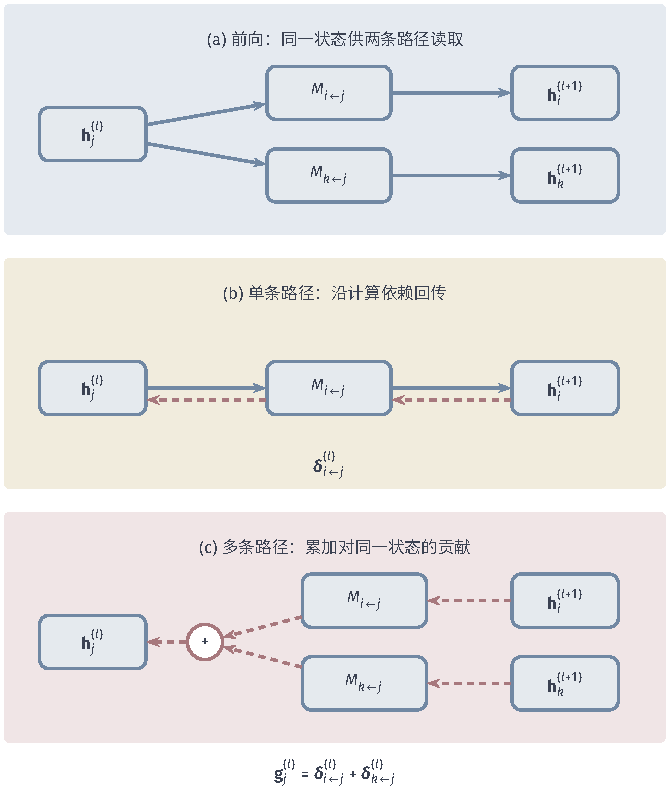
\includegraphics[width=113.404mm]{figures/05-neural-network-models/00-shared/tikz/gnn-backpropagation/figure.pdf}
  \caption{同一节点状态沿两条发送路径收到的梯度贡献。（a）只画前向分叉；（b）跟踪接收节点$i$的回传，消息梯度经发送端Jacobian的转置回到节点$j$；（c）在$+$处累加$i$、$k$两条路径的贡献，记为$\bm g_{j,\mathrm{send}}^{(l)}$。实线表示前向计算，红色虚线表示导数路径。图中贡献和只包含所示的两条发送路径，省略其他消息、自身更新、接收端路径和任务输出头；反向依赖由前向读取决定，不要求原图存在反向边。}
  \label{fig:gnn-backpropagation}
\end{figure*}
\FloatBarrier

状态梯度继续传向上一轮，共享参数的梯度则汇集为本次优化器更新的输入。以一层线性消息$\bm{m}_{i\leftarrow j}=\bm{W}\bm{h}_j$为例，$\bm{W}\in\mathbb{R}^{r_l\times m_l}$，接收端回传的消息梯度给发送端贡献$\bm{W}^{\top}\bm{\delta}_{i\leftarrow j}$，并给权重贡献一个外积。因此
\begin{equation}
  \frac{\partial L}{\partial\bm{W}}
    =\sum_{(j\to i)\in E}
      \bm{\delta}_{i\leftarrow j}\bm{h}_j^{\top}\text{。}
  \label{eq:gnn-shared-gradient}
\end{equation}
跨轮共享$\bm{W}$时，还要对轮次求和。节点更新、输入编码及输出头中的共享参数使用同样规则，正则项的导数另加到相应参数。各边、各轮的贡献汇集后，优化器更新这一份共享权重。

\begin{example}[无标签节点怎样得到梯度]
\label{ex:gnn-unlabeled-gradient}
沿用示例~\ref{ex:gnn-two-rounds}的两轮平均，只在节点1设置目标0，取$L=\tfrac12(h_1^{(2)})^2$。此处状态与梯度都是标量，记$g_i^{(l)}=\partial L/\partial h_i^{(l)}$。由$h_1^{(2)}=3/4$，最终轮梯度为$(3/4,0,0)$。节点1的第二轮输出平均了上一轮节点1和2的状态，故
\[
  \bm{g}^{(1)}=(3/8,3/8,0)^{\top},\qquad
  \bm{g}^{(0)}=(5/16,5/16,1/8)^{\top}\text{。}
\]
例如节点3没有标签，却通过节点2影响节点1；它在初始轮收到的梯度为$(3/8)\times(1/3)=1/8$。由于$h_3^{(0)}=x_3$，这个数值是损失$L$对初始属性$x_3$的导数。

预测量$h_1^{(2)}$对同一输入的导数需要单独区分。节点3的初始属性先以系数$1/3$进入$h_2^{(1)}$，再以系数$1/2$进入$h_1^{(2)}$，所以
\[
  \frac{\partial h_1^{(2)}}{\partial x_3}
    =\frac12\times\frac13=\frac16,\qquad
  \frac{\partial L}{\partial x_3}
    =\frac{\partial L}{\partial h_1^{(2)}}
      \frac{\partial h_1^{(2)}}{\partial x_3}
    =\frac34\times\frac16=\frac18\text{。}
\]
前者衡量预测对输入属性的敏感度；后者还计入当前预测与目标0的偏差$3/4$，衡量的是损失的敏感度。这里没有可学习的传播参数，例子只核对状态及输入的导数；当前任务更新的参数范围仍由模型定义。
\end{example}

\subsubsection{训练批次与信息范围}
\label{sec:gnn-training-batches}

图训练有一个前几章没有的特殊问题：计算一个节点的表示，需要它的邻居，而邻居又需要它们的邻居……那么训练时到底要载入多大一片图？几种做法对应不同的信息范围和计算代价，需要先分清。

\term{全图训练}（full-graph training）在每次前向计算中读取完整的训练可见图，再只在受监督的位置计算损失。单图节点分类时可以只抽取一批标签位置，却仍要计算全图的节点表示——这与只读取部分结构的训练不同。若手上是许多独立小图（如一批分子），可以用块对角邻接矩阵把它们拼成一张互不连通的大图统一计算，读出时再按图归属分别聚合，保证一个分子的节点不会“看到”另一个分子。

大图上$L$跳邻域会随层数指数膨胀（一个高度数节点的邻居的邻居很快就覆盖大半张图），全图计算的显存和时间都可能不可承受。\term{邻居采样}（neighbor sampling）为本批目标节点逐层只随机选取有限个邻居，在采出的计算图上前向和反向：每层最多取$s$个邻居时，未经去重的展开规模约为$1+s+\cdots+s^L$。采样限制了每个节点的分支数，但多层递推仍会逐层展开这些分支。需要注意一个常被忽略的偏差问题：均匀采样的均值可以无偏估计\emph{一次固定的}邻域平均，但非线性更新之后，“先采样再过网络”的预测及其梯度通常\emph{不再}是全图结果的无偏估计；归一化和多层抽样会进一步改变计算。

\term{子图训练}（subgraph training）则直接抽取一部分节点及其边，在这张子图内完成多轮传播。它便于让多个目标节点共享中间计算，但截断边界会丢掉来自外围的消息；若希望完整保留目标节点的$L$跳邻域，可以把外围节点作为上下文纳入。采样误差、边界缺失和标签抽样是三种不同的误差来源，不能混为一谈。

数据的\emph{可见范围}还取决于任务设定，这直接影响训练是否“合法”。\term{直推学习}（transductive learning）针对训练时就已存在的一批对象预测其未知标签：例如引用网络的全部结构和论文特征在训练时都可见，只是部分节点不给标签——测试节点的特征和连接可以参与前向编码，唯独不用它们的标签。\term{归纳学习}（inductive learning）则要求把规则用到训练时\emph{从未见过}的新节点或新图上（如给刚发表的论文、新增的分子分类）。共享消息函数两种设定都适用，因为参数随对象复用是计算结构的性质；但二者评估的泛化能力不同，必须用对应的数据划分来检验。

无论哪种设定，每次更新都应明确三件事：可见图是哪些、输入特征可见到什么程度、监督集合包含谁。对连接预测，还必须在编码图中移除待评估的目标边及其副本（否则模型直接“读到”了要预测的连接，等于漏题）；对动态预测，结构和属性只能来自预测时刻之前。

\subsubsection{参数更新与收敛条件}
\label{sec:gnn-optimization-convergence}

反向传播给出当前参数下的导数，优化器才决定怎样改变参数。将全部可学习参数记为$\bm{\theta}\in\mathbb{R}^{p}$，固定数据与可见图，记训练损失加正则项为$J(\bm{\theta})$。一次普通梯度更新为
\begin{equation}
  \bm{\theta}^{(t+1)}=\bm{\theta}^{(t)}
    -\eta_t\widehat{\bm{g}}^{(t)}\text{，}
  \label{eq:gnn-parameter-update}
\end{equation}
$t$是优化器更新次数，与传播轮次$l$不同；$\eta_t>0$是学习率。全目标求导时$\widehat{\bm{g}}^{(t)}=\nabla J(\bm{\theta}^{(t)})$，抽批次时则是相应计算得到的梯度估计。同一次更新的前向和反向使用同一份参数。旧梯度累积按训练规则清除或保留，本批贡献再求和或按约定平均，随后进入优化器。

网络的多层复合、消息函数和输出头通常使$J$非凸。训练进展可以由损失值、梯度尺度或参数变化测量；达到驻点与找到全局最小值又有不同的条件。共享参数与归一化会改变目标及传播尺度，求解保证仍需由完整优化问题建立。

一个有条件的结果说明梯度法为什么可能稳定降低目标。假定$J$有下界$J_{\inf}$，且梯度是$\beta$-Lipschitz的，即$\lVert\nabla J(\bm{u})-\nabla J(\bm{v})\rVert_2\leq\beta\lVert\bm{u}-\bm{v}\rVert_2$，其中$\beta>0$。沿连接两参数的线段积分梯度，可得
\[
  J(\bm{u})\leq J(\bm{v})+
  \langle\nabla J(\bm{v}),\bm{u}-\bm{v}\rangle
  +\frac{\beta}{2}\lVert\bm{u}-\bm{v}\rVert_2^2\text{。}
\]
若使用完整梯度与固定学习率$0<\eta\leq1/\beta$，代入式\eqref{eq:gnn-parameter-update}即得到
\begin{equation}
  \begin{aligned}
    J(\bm{\theta}^{(t+1)})
      &\leq J(\bm{\theta}^{(t)})
        -\frac{\eta}{2}\lVert\nabla J(\bm{\theta}^{(t)})\rVert_2^2,\\
    \min_{0\leq t<T}\lVert\nabla J(\bm{\theta}^{(t)})\rVert_2^2
      &\leq\frac{2[J(\bm{\theta}^{(0)})-J_{\inf}]}{\eta T}\text{。}
  \end{aligned}
  \label{eq:gnn-gradient-descent-bound}
\end{equation}
第二行由第一行对$T$次更新求和得到，$T$是优化步数。它控制前若干次更新中最小的梯度范数平方；在这些假设下，各迭代点的梯度范数也趋于零。参数序列是否有极限、驻点是否全局最优，还需进一步条件。ReLU与最大聚合具有不可微位置，实际目标的有限平滑常数$\beta$也需要在所分析区域建立，光滑结论的适用范围由此确定。

抽样梯度还增加了波动。若它在给定参数下无偏、方差有统一上界，并满足相应光滑性及下界条件，递减学习率可以控制梯度噪声。经典条件包括$\sum_t\eta_t=\infty$和$\sum_t\eta_t^2<\infty$，能保证按学习率加权的期望梯度平方范数平均值趋于零。这个指标描述迭代过程的加权平均，参数极限与全局最优另需条件。固定非零学习率通常只能保证平均梯度大小受噪声项控制，单步损失不必持续下降。Bottou等的分析明确区分了这两种情形\scite{bottou2018optimization} 在固定编码图上，均匀抽取标签位置并按目标正确缩放，可以保持完整标签平均损失的无偏梯度；邻居采样经过多层非线性却未必如此。标签抽样和邻域抽样可能对应不同梯度对象，收敛分析随实际目标和更新规则确定；自适应优化器也需要对应的条件。

实际停止可结合最大步数、在固定评估计算上的训练损失与梯度范数，以及验证指标的早停。传播深度、初始化、度归一化、残差与门控会影响链式Jacobian的尺度，从而影响梯度过小或过大的程度；学习率和优化器也须与该尺度匹配。可以据实际梯度和目标变化检验这些设计对训练条件的影响。固定参数下的状态迭代是否收敛则是另一问题，第~\ref{sec:gnn-state-convergence}节讨论其充分条件；新对象上的误差则由匹配预测设定的数据另行检验。

\section{卷积图神经网络}
\label{sec:gnn-convolutional}

消息传递已经能处理任意图，但“每个节点用什么权重聚合邻居”仍可进一步设计。本章标题中的“图卷积”，指的是把第3章卷积网络在规则网格上\emph{共享滤波系数}的思想推广到不规则图：在图像上，每个位置都用同一组核系数，因为“右边一格”在任何位置含义相同；图上没有统一的相对坐标，节点的邻居不仅数量不同、没有次序，编号差也不代表距离。于是“卷积”在图上必须重新定义——它不再对应一个滑动窗口，而是一个\emph{作用在图信号上的共享传播算子}。

这种推广有两个互补的思考入口，初学时可以分别理解、最终会合到同一处。
\begin{itemize}
  \item \textbf{谱域入口}沿用信号处理中“卷积定理”的形式：先把节点上的信号分解成若干种振荡模式（图的傅里叶基），在模式空间里逐分量缩放，再变换回来。它在数学上优雅，但要先求出整张图的特征向量，计算昂贵且难以跨图迁移。
  \item \textbf{空域入口}沿用消息传递的直觉：沿每个节点的邻域，用同一套规则组合邻居、再做与次序无关的聚合。它直观、稀疏、易扩展。
\end{itemize}
\term{图卷积}（graph convolution）正是这两者的统称；本节会看到，当谱域滤波器取为拉普拉斯的多项式时，两个入口在数学上完全等价——\emph{在频率空间设计滤波器，等价于在节点邻域上做有限跳的稀疏传播}。一般图缺少网格上的统一平移，因此“卷积”由图关系上的算子定义，再由该算子决定传播行为和计算代价。

一个线性图滤波器可以把两种入口联系起来。令$\bm{Q}\in\mathbb{R}^{n\times n}$是给定的局部传播矩阵，非对角非零元只位于相邻节点间；邻接矩阵就是一个选择。对$\bm{H}\in\mathbb{R}^{n\times d_{\mathrm{in}}}$，可定义
\begin{equation}
  \bm{Z}=\sum_{k=0}^{K}\bm{Q}^{k}\bm{H}\bm{W}_k,
  \qquad \bm{W}_k\in\mathbb{R}^{d_{\mathrm{in}}\times d_{\mathrm{out}}}\text{。}
  \label{eq:gnn-polynomial-convolution}
\end{equation}
其中$\bm{Q}^0=\bm{I}_n$，$\bm{Z}\in\mathbb{R}^{n\times d_{\mathrm{out}}}$；$k=0$处理自身，$k\geq1$组织至多$k$跳内经传播到达的信息。$\bm{W}_k$在所有节点共享，并不为每条具体路径另设参数。计算时递推$\bm{H}_0=\bm{H}$、$\bm{H}_k=\bm{Q}\bm{H}_{k-1}$，累加$\bm{H}_k\bm{W}_k$，无需显式形成通常更稠密的$\bm{Q}^k$。非线性激活再作用于$\bm{Z}$，多层这样的计算构成网络。

式\eqref{eq:gnn-polynomial-convolution}如何包含普通卷积，可以在周期的一维有向网格上看清。取移位矩阵$\bm{T}$，满足$(\bm{T}\bm{x})_i=x_{i-1}$，下标按周期返回；则单通道有限核的循环卷积是$\sum_{r=-K}^{K}w_r\bm{T}^{r}\bm{x}$。不同偏移对应重复移位或反向移位。一般图改用邻接或拉普拉斯等关系算子组织传播。单个无向对称算子把两方向按同一关系处理；带方向或类型差别的核则需要相应的关系信息及不同的关系算子。

共享还必须服从重编号。若$\bm{Q}'=\bm{P}\bm{Q}\bm{P}^{\top}$、$\bm{H}'=\bm{P}\bm{H}$，则$\bm{Z}'=\bm{P}\bm{Z}$，因为$(\bm{P}\bm{Q}\bm{P}^{\top})^k\bm{P}=\bm{P}\bm{Q}^k$。这使局部组合不依赖节点保存次序。但一般消息传递比线性卷积更广：注意力或非线性边消息可以让权重依赖输入，不必对应某个固定的线性频率响应。下面分别从图信号的模式与邻域计算定义具体算子，再比较两者的联系和适用条件。

\subsection{谱域图神经网络}
\label{sec:gnn-spectral}

\subsubsection{图拉普拉斯与图傅里叶变换}
\label{sec:gnn-graph-fourier}

要理解谱域图卷积，先回答“图上的频率是什么”。把每个节点上的一个标量看成图信号，直觉上：如果相邻节点的取值都差不多（信号在边上变化平缓），这是\emph{低频}成分；如果相邻节点取值剧烈跳变（信号在每条边上都在振荡），这是\emph{高频}成分。图拉普拉斯正是一个度量“相邻差异总和”的算子，它可以把任意信号分解成从平缓到剧烈的一系列正交模式；本节要学习的是如何对不同模式施加不同的响应（比如平滑去噪就保留低频、抑制高频）。

记$d_i=\sum_j\bm A_{i,j}$为节点度，$\bm D=\operatorname{diag}(d_1,\ldots,d_n)$为度矩阵。
节点度差异较大时，常用\term{对称归一化拉普拉斯}（symmetric normalized Laplacian），以免高度数节点主导一切。
本节为简化推导，假定所有节点$d_i>0$，令
\begin{equation}
  \bm{L}=\bm{I}_n-\bm{D}^{-1/2}\bm{A}\bm{D}^{-1/2}
    =\bm{U}\bm{\Lambda}\bm{U}^{\top}\text{。}
  \label{eq:gnn-laplacian-spectrum}
\end{equation}
$\bm{U}\in\mathbb{R}^{n\times n}$的列$\bm{u}_k$是正交特征向量，$\bm{\Lambda}$的对角元素$\lambda_k\in[0,2]$按升序排列。归一化后的能量比较$x_i/\sqrt{d_i}$与$x_j/\sqrt{d_j}$，因此零频模式在每个连通分量内与$\sqrt{d_i}$成比例，未必是常量；不同分量可以具有不同的比例系数。图连通时，零特征空间才只有这一个方向。存在孤立节点时须另规定归一化约定，或加自环后再定义相应算子。

在当前归一化拉普拉斯的图傅里叶坐标$\widehat{\bm x}=\bm U^\top\bm x$中，
让频率响应$g_{\bm\theta}(\lambda)$随训练参数改变，得到可学习的谱滤波：
\begin{equation}
  \bm{y}=\bm{U}g_{\bm{\theta}}(\bm{\Lambda})\bm{U}^{\top}\bm{x}
    =g_{\bm{\theta}}(\bm{L})\bm{x}\text{。}
  \label{eq:gnn-spectral-filter}
\end{equation}
图~\ref{fig:gnn-spectral-filter}显示这三步。谱域图卷积沿用傅里叶域逐模式相乘的形式；图的连接决定这些模式，所以滤波的含义由图谱而非普通空间偏移给出。

\begin{figure*}[htb]
  \centering
  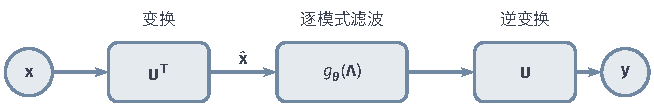
\includegraphics[width=110.793mm]{figures/05-neural-network-models/00-shared/tikz/gnn-spectral-filter/figure.pdf}
  \caption{谱滤波的计算路径。节点信号$\bm{x}$经$\bm{U}^{\top}$分解为图傅里叶系数，每个模式由$g_{\bm{\theta}}(\lambda_k)$调整，再经$\bm{U}$还原为节点信号。左、右两端使用同一张图和同一节点顺序；中间向量的下标表示频率模式。}
  \label{fig:gnn-spectral-filter}
\end{figure*}
\FloatBarrier

\begin{example}[三节点路径上的低频模式]
\label{ex:gnn-low-frequency}
沿用路径$1-2-3$，此处不加自环，度为$(1,2,1)$。归一化拉普拉斯的特征值为$0,1,2$，可取
\[
  \bm{u}_1=\tfrac12(1,\sqrt2,1)^{\top},\quad
  \bm{u}_2=\tfrac{1}{\sqrt2}(1,0,-1)^{\top},\quad
  \bm{u}_3=\tfrac12(1,-\sqrt2,1)^{\top}\text{。}
\]
输入$\bm{x}=(1,0,2)^{\top}$的三个系数为$3/2,-1/\sqrt2,3/2$。若只保留零频模式，输出为$(3/4,3\sqrt2/4,3/4)^{\top}$。中间节点的数值较大，恰是度归一化后的平滑，而不是普通算术平均。
\end{example}

\subsubsection{Spectral CNN：直接学习频率响应}
\label{sec:gnn-spectral-cnn}

Bruna等的Spectral CNN把谱滤波放入多通道网络。对输入通道$a$与输出通道$b$，可以学习一个对角滤波器$\bm{\Theta}_{a,b}$，用$\bm{U}\bm{\Theta}_{a,b}\bm{U}^{\top}$变换对应信号，再累加通道并使用非线性。完整谱上的自由响应需要每通道对$n$个参数；原工作还用少量样条系数插值得到平滑响应，减少参数自由度\scite{bruna2014spectral}

固定图与傅里叶基时，前向计算是矩阵乘法，滤波参数可按链式法则求导。例如单通道$\bm{y}=\bm{U}\operatorname{diag}(\bm{\theta})\widehat{\bm{x}}$，上游梯度为$\bm{v}=\partial L/\partial\bm{y}$，则$\partial L/\partial\theta_k=(\bm{U}^{\top}\bm{v})_k\widehat x_k$。通道与样本之间共享参数时，对相应贡献求和即可。

直接使用稠密$\bm{U}$需要$O(n^2)$的单信号变换和存储，完整稠密特征分解的常规代价为$O(n^3)$。只保留部分特征向量可以改变代价，但也限制了可用模式。自由频率响应还可能对应全图稠密算子，读取范围要由实际响应检验；有限跳数局部性需要另加结构。

对新图，特征值与特征向量都会变化，按旧图谱索引学习的自由系数没有自然的一一对应。特征向量的符号在$\bm{U}\bm{\Theta}\bm{U}^{\top}$中相消，但重特征值对应的子空间还可以旋转；若该子空间内使用不同自由系数，算子就依赖具体基的选择。由同一个标量函数$g(\lambda)$定义响应，能够消除这种基选择歧义；跨图迁移的预测效果仍需另行验证。

\subsubsection{ChebNet：用多项式实现局部滤波}
\label{sec:gnn-chebnet}

Spectral CNN虽然给了图卷积一个干净的谱定义，却有两个致命的工程问题：要显式求出并保存稠密的特征基$\bm U$（代价$O(n^3)$、存储$O(n^2)$），而且这些基是\emph{针对某一张具体的图}算出来的——在一张引用图上学到的频率系数，换一张结构不同的图就无处对齐，无法迁移。解决思路来自信号处理中的一个事实：\emph{如果让频率响应$g$是拉普拉斯矩阵$\bm L$的多项式，那么$g(\bm L)\bm x$根本不需要显式的$\bm U$，只用稀疏的矩阵—向量乘法就能算}；而且多项式系数只描述“怎么对$\bm L$组合”，可以直接拿到另一张图上用它自己的$\bm L$重新计算。ChebNet用\term{切比雪夫多项式}（Chebyshev polynomial）来参数化这个响应，既有良好的数值性质又能控制阶数。设$\lambda_*>0$是拉普拉斯谱的上界，令$\widetilde{\bm{L}}=2\bm{L}/\lambda_*-\bm{I}_n$，把谱放到$[-1,1]$；归一化拉普拉斯可取$\lambda_*=2$。约定$K$为最高次数，则
\begin{equation}
  g_{\bm{\theta}}(\bm{L})\bm{x}
    =\sum_{k=0}^{K}\theta_k T_k(\widetilde{\bm{L}})\bm{x}\text{，}
  \label{eq:gnn-chebyshev-filter}
\end{equation}
其中$T_0(z)=1$、$T_1(z)=z$、$T_k(z)=2zT_{k-1}(z)-T_{k-2}(z)$。有些文献用$K$表示项数，此时最高次数为$K-1$，阅读时须核对约定\scite{defferrard2016chebnet}

令$\bm{z}_k=T_k(\widetilde{\bm{L}})\bm{x}$，即可用$\bm{z}_0=\bm{x}$、$\bm{z}_1=\widetilde{\bm{L}}\bm{x}$以及$\bm{z}_k=2\widetilde{\bm{L}}\bm{z}_{k-1}-\bm{z}_{k-2}$递推。整个过程只需要稀疏矩阵乘向量；单通道的$K\geq1$阶计算量为$O(K(n+e))$，无需构造$\bm{U}$。反向传播也经过这些稀疏乘法，系数梯度为$\bm{v}^{\top}\bm{z}_k$。

多项式为何局部，可以从矩阵乘法看出。$\bm{L}$的非对角非零元只连接相邻节点，一次相乘至多走一条边；$\bm{L}^k$至多连接$k$跳以内。故式\eqref{eq:gnn-chebyshev-filter}在一层中读取至多$K$跳邻域。多通道形式为$\bm{Y}=\sum_{k=0}^{K}T_k(\widetilde{\bm{L}})\bm{X}\bm{\Theta}_k$，$\bm{\Theta}_k\in\mathbb{R}^{d_{\mathrm{in}}\times d_{\mathrm{out}}}$，参数量为$(K+1)d_{\mathrm{in}}d_{\mathrm{out}}$，不随$n$增加。

这些系数描述同一个多项式，所以可以在另一张图上重新构造拉普拉斯并使用它们，无需对齐特征向量。频率分布与任务关系随图改变，预测质量也需在新图上检验。若使用的谱上界过小，使缩放后的特征值落到$[-1,1]$以外，高次多项式还可能迅速放大误差。

\subsection{空域图神经网络}
\label{sec:gnn-spatial}

ChebNet已经把谱卷积化成了邻域上的稀疏传播，空域方法则干脆直接在消息传递框架里设计聚合规则，不再借助傅里叶语言。下面四个经典模型可以理解为针对同一个朴素邻域平均的四次“挑刺”，每个解决一个具体缺陷：GCN解决\emph{度数不均导致的尺度问题}（用归一化加权而非简单平均），GraphSAGE解决\emph{大图算不动、新节点无法归纳}的问题（采样+拼接自身），GAT解决\emph{归一化权重与内容无关}的问题（按邻居相关性动态加权），GIN则解决\emph{平均/最大聚合会丢掉邻居数量差异}的表达能力问题（用求和保多重集）。它们共享前面的输出与反向传播机制，主要差别只在聚合和更新两步。

\subsubsection{GCN：归一化的邻域传播}
\label{sec:gnn-gcn}

先看最简单的邻域平均会有什么问题。直接把自己和所有邻居的特征相加，度数很高的节点（一个连了上千邻居的枢纽）聚合出的数值会远大于度数低的节点，数值尺度随度数剧烈波动，训练难以稳定。\term{图卷积网络}（graph convolutional network, GCN）在本节特指Kipf与Welling提出的层形式，它的核心就是一个\emph{按两端度数归一化}的传播矩阵：加入自环$\widetilde{\bm{A}}=\bm{A}+\bm{I}_n$（让节点也读取自身），令$\widetilde d_i=\sum_j\widetilde{\bm{A}}_{i,j}$，定义
\begin{equation}
  \bm{S}=\widetilde{\bm{D}}^{-1/2}\widetilde{\bm{A}}\widetilde{\bm{D}}^{-1/2},
  \qquad
  \bm{H}^{(l+1)}=\sigma\!\left(\bm{S}\bm{H}^{(l)}\bm{W}^{(l)}\right)\text{。}
  \label{eq:gnn-gcn-layer}
\end{equation}
$\bm{H}^{(l)}\in\mathbb{R}^{n\times m_l}$按行存放状态，$\bm{H}^{(0)}=\bm{X}$；$\bm{W}^{(l)}\in\mathbb{R}^{m_l\times m_{l+1}}$变换特征通道，$\sigma$逐坐标作用。采用行存放的矩阵形式时，节点列向量的变换对应$(\bm{W}^{(l)})^{\top}\bm{h}_i^{(l)}$。原始层式省略偏置，增加共享偏置不会改变置换等变性。

从节点$j$到$i$的消息系数为$\widetilde{\bm{A}}_{i,j}/\sqrt{\widetilde d_i\widetilde d_j}$，同时计入边权以及接收端与发送端的度。边权为1时，才简化为$1/\sqrt{\widetilde d_i\widetilde d_j}$。这个组合按两端度归一化；$\bm{S}$的行和未必等于1，数值因此不同于算术平均。沿用三节点无权路径与输入$(1,0,2)^{\top}$，取单位特征变换和恒等激活，得到
\begin{equation}
  \bm{S}=\begin{pmatrix}
    1/2&1/\sqrt6&0\\
    1/\sqrt6&1/3&1/\sqrt6\\
    0&1/\sqrt6&1/2
  \end{pmatrix},\qquad
  \bm{S}\bm{x}=\begin{pmatrix}1/2\\3/\sqrt6\\1\end{pmatrix}\text{。}
  \label{eq:gnn-gcn-example}
\end{equation}
这一结果与示例~\ref{ex:gnn-two-rounds}的平均不同，差别来自归一化规则。

它与谱域方法的联系可以直接推导。对不加自环的归一化拉普拉斯，ChebNet取$K=1$及$\lambda_*=2$时，$\widetilde{\bm{L}}=-\bm{D}^{-1/2}\bm{A}\bm{D}^{-1/2}$。再约束$\theta_0=-\theta_1=\theta$，得到$\theta(\bm{I}_n+\bm{D}^{-1/2}\bm{A}\bm{D}^{-1/2})\bm{x}$。GCN进一步以加自环后重新计算度的$\bm{S}$替换括号内算子，限制反复传播的尺度。这一步更换了传播算子及其度归一化；原论文称其为重新归一化技巧\scite{kipf2017gcn}

固定结构时，GCN的梯度也可写清。记$\bm{Z}=\bm{S}\bm{H}\bm{W}$，$\bm{\Delta}=\partial L/\partial\bm{Z}$，则
\begin{equation}
  \frac{\partial L}{\partial\bm{W}}=(\bm{S}\bm{H})^{\top}\bm{\Delta},\qquad
  \frac{\partial L}{\partial\bm{H}}=\bm{S}^{\top}\bm{\Delta}\bm{W}^{\top}\text{。}
  \label{eq:gnn-gcn-backprop}
\end{equation}
激活的导数已并入$\bm{\Delta}$。不学习邻接关系时，$\bm{S}$作为给定算子；学习边权或建图规则时，才需进一步计算结构相关梯度。

标准GCN直接混合相邻节点的变换特征。相邻对象与预测目标相关时，这种共享聚合可以提供有用信息；相邻节点常具有不同标签或关系语义时，混合也可能损失区分所需的特征。共享权重可以接新图重建的传播算子；归纳表现需要按照新图的信息范围和数据检验，原始实验设定只说明其当时的任务。

\subsubsection{GraphSAGE：采样并学习邻域组合}
\label{sec:gnn-graphsage}

GCN仍有两个适用边界：它一次要读取每个节点的\emph{全部}邻居，在百万节点的大图上为一批目标节点展开完整邻域代价过高；而且它的计算依赖整张固定的图，遇到训练后才新加入的节点就无法直接套用（不支持归纳）。GraphSAGE的改造有两点：一是每轮只\emph{随机采样}固定数量的邻居，把计算量钉死；二是把“自身表示”和“邻居聚合结果”先\emph{分开}再拼接，让网络用不同权重分别决定保留多少自身信息、吸收多少邻域信息。这样新节点到达时，只要按相同规则采样其邻居、读取可用属性即可生成表示，而不必依赖它在训练图中的编号。以平均聚合为例，从$N(i)$中取$S_i^{(l)}$，令
\begin{equation}
  \begin{aligned}
    \bm{u}_i^{(l)}&=\frac{1}{|S_i^{(l)}|}\sum_{j\in S_i^{(l)}}\bm{h}_j^{(l)},\\
    \bm{h}_i^{(l+1)}&=\sigma\!\left(
      \bm{W}^{(l)}[\bm{h}_i^{(l)};\bm{u}_i^{(l)}]+\bm{b}^{(l)}\right)\text{。}
  \end{aligned}
  \label{eq:gnn-graphsage}
\end{equation}
分号表示向量拼接，此处$\bm{W}^{(l)}\in\mathbb{R}^{m_{l+1}\times2m_l}$。自身和邻居先分开，再由不同的权重块组合；原算法还可对输出作$\ell_2$归一化，零向量需要单独处理\scite{hamilton2017graphsage}

聚合器也可对邻居先作共享前馈变换，再取逐坐标最大值。平均保留总体水平，最大池化突出某种响应是否出现。原论文还试验了对随机邻居顺序使用LSTM的聚合器。一次LSTM输出取决于所抽顺序；对称聚合直接消除枚举次序，随机顺序方案则需说明对称化或输出分布的口径。

训练时采样所需邻域，计算节点或关系任务的损失，联合更新聚合器、组合矩阵及输出头。预测新节点时沿相同规则读取可用特征与邻域，不必为它单独学习一个节点编号嵌入。新节点可提供的属性与邻域决定表示的信息来源。只使用旧节点编号时，可迁移属性不足；新节点缺乏特征或邻居时也需要相应初态或补充输入。

\subsubsection{GAT：根据内容调整邻居权重}
\label{sec:gnn-gat}

GCN的归一化权重只由图的\emph{拓扑}（各节点的度）决定：一旦图固定，某个邻居占多大权重就固定了，与邻居当前的特征、与当前任务是否相关完全无关。但直觉上，聚合时理应更重视\emph{内容上更相关}的邻居。\term{图注意力网络}（graph attention network, GAT）借用第4章的注意力思想：用节点特征临时为每条边计算一个权重，再在图约束的可见邻域内归一化加权——注意这里的可见范围仍由边严格限定（不是任意两节点都能注意），这是它与Transformer自注意力的关键区别。对一个注意力头，令$\bm{z}_i=\bm{W}\bm{h}_i$，其中$\bm{W}\in\mathbb{R}^{m'\times m}$，则
\begin{equation}
  \begin{aligned}
    e_{i,j}&=\operatorname{LeakyReLU}
      \!\left(\bm{a}^{\top}[\bm{z}_i;\bm{z}_j]\right),\\
    \alpha_{i,j}&=\frac{\exp(e_{i,j})}
      {\sum_{k\in N(i)\cup\{i\}}\exp(e_{i,k})},\\
    \bm{h}'_i&=\sigma\!\left(\sum_{j\in N(i)\cup\{i\}}
      \alpha_{i,j}\bm{z}_j\right)\text{。}
  \end{aligned}
  \label{eq:gnn-gat}
\end{equation}
$\bm{a}\in\mathbb{R}^{2m'}$是共享评分参数；$e_{i,j}$是标量得分，与本章的边数$e$不同。Softmax只在节点$i$的可见邻域内归一化，所有节点使用同一评分函数，所以邻居重排只重排对应权重\scite{velickovic2018gat}

多头注意力分别学习变换和评分，在隐藏层拼接结果，或在输出层取平均。训练时梯度同时通过值向量和权重；若把权重当作常量，就漏掉了评分函数对损失的影响。固定每头宽度时，增加头数还会增加总宽度和参数量，相同宽度预算下的比较需相应分配各头维度。

与前章的循环注意力一样，GAT把“计算权重”和“读取信息”分开；区别是可见位置由图的邻接关系约束。原始GAT的评分使用线性拼接，若将$\bm{a}$拆成两部分，得分是单调激活作用于一个接收端项与一个发送端项之和。因此，在固定候选邻居特征下，邻居排序不能仅靠改变接收端特征任意翻转。这说明原始评分虽随内容产生权重，候选排序仍受到该加性结构的限制。

注意力调整可见邻居之间的相对影响，单轮读取范围仍由图限定。归一化权重描述一次聚合中的数值比例，预测作用还取决于表示内容、评分变化及后续计算；解释或因果结论需要另外的证据。

\subsubsection{GIN：保留邻域多重集合的差别}
\label{sec:gnn-gin}

前几种模型默认用平均（或最大）聚合，但前面强调过，多重集合里\emph{元素的重复次数是信息}；平均和最大恰恰会系统性地抹掉这种计数差别。考虑两个邻域：$\{\!\{1,1\}\!\}$（两个邻居都取1）与$\{\!\{1,1,1\}\!\}$（三个邻居都取1），它们的平均都是1、最大也都是1——度数不同这个事实在聚合后彻底消失。再如$\{\!\{0,2\}\!\}$与$\{\!\{1,1\}\!\}$，连求和都相同（都等于2）。要区分这些结构，必须先选用能保留计数的聚合（求），再配足够灵活的特征映射把和中混在一起的差异分开。图~\ref{fig:gnn-aggregation}展示第一种信息损失。

\begin{figure*}[htb]
  \centering
  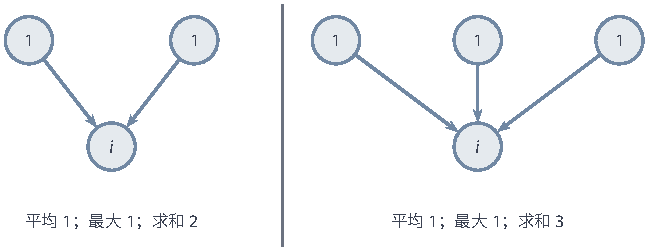
\includegraphics[width=109.792mm]{figures/05-neural-network-models/00-shared/tikz/gnn-aggregation/figure.pdf}
  \caption{聚合如何保留或丢掉重复次数。两个邻域分别含两个和三个数值为1的邻居。平均与最大值都产生1，求和分别产生2和3。图只比较固定标量消息；求和本身也不能区分所有不同多重集合，还需要合适的特征映射。}
  \label{fig:gnn-aggregation}
\end{figure*}
\FloatBarrier

\term{图同构网络}（graph isomorphism network, GIN）使用求和聚合与前馈更新：
\begin{equation}
  \bm{h}_i^{(l+1)}=\operatorname{MLP}^{(l)}\!\left(
    (1+\epsilon^{(l)})\bm{h}_i^{(l)}
      +\sum_{j\in N(i)}\bm{h}_j^{(l)}\right)\text{，}
  \label{eq:gnn-gin}
\end{equation}
$\epsilon^{(l)}$可以固定或学习，用于区分中心节点与邻居的贡献。参数通过任务损失反向传播；整图读出还可拼接各层节点求和，保留不同传播范围的信息\scite{xu2019gin}

比较两张图时，若存在保持连接关系及给定属性的节点重编号，使两图相互对应，就称它们\term{同构}（isomorphic）。GIN的区分能力通过下面的标记更新检验作比较。衡量其区分能力的一种参照是\term{一维Weisfeiler--Leman检验}（1-dimensional Weisfeiler--Leman test, 1-WL）：从与节点属性一致的初始标记出发，反复用“节点旧标记及邻居标记的多重集合”产生新标记。所比较的图必须使用同一套无冲突标记规则，相同的输入组合得到相同标记，不同组合得到不同标记。每轮比较两图全部节点标记组成的多重集合；只要有一轮不同，就可判为非同构，始终相同时，检验仍留下未判定的图对。

对于只使用节点状态、对称邻域聚合且不引入额外区分信息的消息传递网络，1-WL无法区分的图也不能靠这些更新与节点多重集合读出区分：同标记节点具有同样的邻域标记多重集合，共享计算遂逐轮产生同样的状态。

在可数特征域、邻域大小有界，以及聚合、更新和读出满足相应单射性条件时，求和特征映射可以达到1-WL的区分能力。\term{单射}（injective）表示不同输入不会被映成同一个结果。有限宽度和训练得到的映射，需要按实际输入检查前述特征域与单射条件。

1-WL本身也有边界。六节点环与两个互不连接的三角形都具有六个节点，每个节点度为2。若初始节点特征全部相同，这两张图上的节点在每轮都会收到两个相同状态，任何上述消息传递加节点多重集合读出都无法区分它们。共同的两邻居模式随轮次持续重复，单靠更多轮数仍无法区分。子结构信息、更高阶状态或其他任务输入可以改变这类区分条件；由数据学得的预测质量还由训练与泛化分析评价。

\subsection{谱域与空域的联系、区别及选择}
\label{sec:gnn-spectral-spatial-comparison}

谱域与空域的区别主要在于怎样规定算子，而不是计算一定发生在哪一类存储空间。谱域用$g_{\bm{\theta}}(\lambda)$规定不同变化模式的响应，空域用邻居的选择、消息和聚合规定局部组合。若$g_{\bm{\theta}}$是多项式，$\bm{U}g_{\bm{\theta}}(\bm{\Lambda})\bm{U}^{\top}$等于同一多项式作用于$\bm{L}$，便可完全通过节点域稀疏传播计算。ChebNet由谱域设计、按邻域递推实现，GCN也保留了谱域推导。谱域规定响应，节点域稀疏传播实现它；同一模型由此可以同时具有频率与局部邻域解释。

表~\ref{tab:gnn-spectral-spatial}将显式谱实现与多项式实现分开。比较计算量时固定一张稀疏图与单通道线性传播，不计特征通道变换、消息网络及初次特征分解的代价；任意空域消息网络的成本还取决于其具体函数。
\begin{table*}[htb]
  \centering
  \small
  \begin{tabularx}{\linewidth}{@{}p{17mm}XXX@{}}
    \toprule
    比较方面 & 显式谱基滤波 & 多项式谱滤波 & 局部空域聚合\\
    \midrule
    算子定义 & 在图傅里叶模式上规定响应 & 用低阶多项式参数化响应 & 用邻居消息、权重及更新规定组合\\
    实际计算 & $\bm{U}^{\top}$、对角滤波、$\bm{U}$ & 拉普拉斯的稀疏乘法递推 & 沿可见边计算，再按节点聚合\\
    局部范围 & 自由响应通常涉及全图 & $K$次多项式至多读取$K$跳 & 一轮通常读取一跳；可另加长程边\\
    传播成本 & 稠密基下$O(n^2)$ & $O(K(n+e))$ & 一跳简单聚合为$O(n+e)$\\
    跨图使用 & 按旧谱索引的自由参数缺少自然对应 & 共享多项式系数，在新图重建算子 & 共享消息规则，在新图读取邻域\\
    \bottomrule
  \end{tabularx}
  \caption{谱域与空域图卷积的比较。显式谱基滤波表示直接使用完整图傅里叶基的实现；多项式谱滤波同时具有有限邻域解释。跨图使用一行只说明计算规则能否复用，不能据此保证新图上的预测效果。}
  \label{tab:gnn-spectral-spatial}
\end{table*}
\FloatBarrier

在大图、多个大小不同的图或不断变化的图上，直接依赖完整$\bm{U}$有几项实际困难。特征分解与稠密变换占用时间和存储，图结构改变后还需处理新的谱；按某张图谱索引学习的系数无法直接对应另一张图的模式。一般自由响应又不是严格局部的，一批目标节点可能依赖大量其他节点，难以只取少量邻居完成同一计算。这些条件解释了为何直接使用完整特征基的早期实现较少成为大规模局部模型的计算方式。

沿边的空域计算容易与邻居采样及小批次结合，也便于让消息读取边类型、方向和接收端内容。复杂度在稀疏图与固定宽度下可随边数增长，参数不必随节点数增加。这种组织便于局部计算，优化和信息保留还取决于消息、深度和数据。多项式谱滤波也能绕开显式特征分解、共享局部传播；它与自由谱基实现的成本和读取范围分别比较。

完整谱基、多项式滤波和空域聚合提供了不同的计算取舍，选择时应回到所需关系。若关心图信号哪些频率应保留或抑制，谱响应提供了直接的设计和分析对象；若需要不同边类型、内容相关交互或采样邻域，空域消息规则更便于表达这些计算。固定线性滤波、有限邻域与跨图复用可以同时成立；输入相关的非线性消息则未必是单个固定谱滤波器。比较两类网络时，应同时写清算子定义、实际实现、可见范围和数据条件。

谱滤波的后续研究继续改进参数化与计算方式。2022年的ChebNetII通过切比雪夫插值组织可学习的谱响应，改进原有滤波器的参数化\scite{he2022chebnetii} 2026年的L2G-NET研究图傅里叶变换的结构化分解，用子图谱表示及其组合处理局部与全局信息，针对完整谱变换的成本和局部性提出新的计算方式\scite{fernandez2026l2gnet} 这些工作进一步探索了频率响应、局部传播和全局交互之间的联系，各自的收益需要结合任务与数据检验。

\section{循环图神经网络}
\label{sec:gnn-recurrent}

前面的GCN、GAT等模型为每一“层”学习一组不同参数：第1层和第2层做的是不同变换。但还可以有另一种设计哲学：如果“在图上反复传播并融合邻居信息”这件事本身值得做很多次，为什么每一轮都要用不同的规则？循环图网络让\emph{同一套更新规则在同一张固定的图上反复作用}，像第4章的RNN在时间上共享参数一样，这里在传播轮次上共享参数。务必先澄清一个易混点：本节的“轮次”是算法内部的迭代次数，\emph{图本身并不随轮次改变}（输入始终是同一张图）；现实中随时间演化的动态图是另一回事，在第~\ref{sec:gnn-dynamic}节处理。

\subsection{网络结构}
\label{sec:gnn-recurrent-structure}

\term{循环图神经网络}（recurrent graph neural network）在同一图上反复更新所有节点的隐状态，直到满足停止条件或达到预定轮数。将全部状态按节点堆成列向量$\bm{h}^{(t)}\in\mathbb{R}^{nm}$，令参数向量为$\bm{\theta}\in\mathbb{R}^{p}$，可写为
\begin{equation}
  \bm{h}^{(t+1)}=F_{\bm{\theta}}(\bm{h}^{(t)};\mathcal{G},\bm{X}),
  \qquad \widehat{\bm{y}}=g_{\bm{\theta}}(\bm{h}^{(T)})\text{。}
  \label{eq:gnn-recurrent-update}
\end{equation}
$F_{\bm{\theta}}$内部仍包含共享消息、聚合与节点更新；分号后的图与属性在各轮固定。图~\ref{fig:gnn-recurrent}显示同一规则的多次调用，每次调用的状态值不同。跨轮共享还要求相应状态维度兼容。

\begin{figure*}[htb]
  \centering
  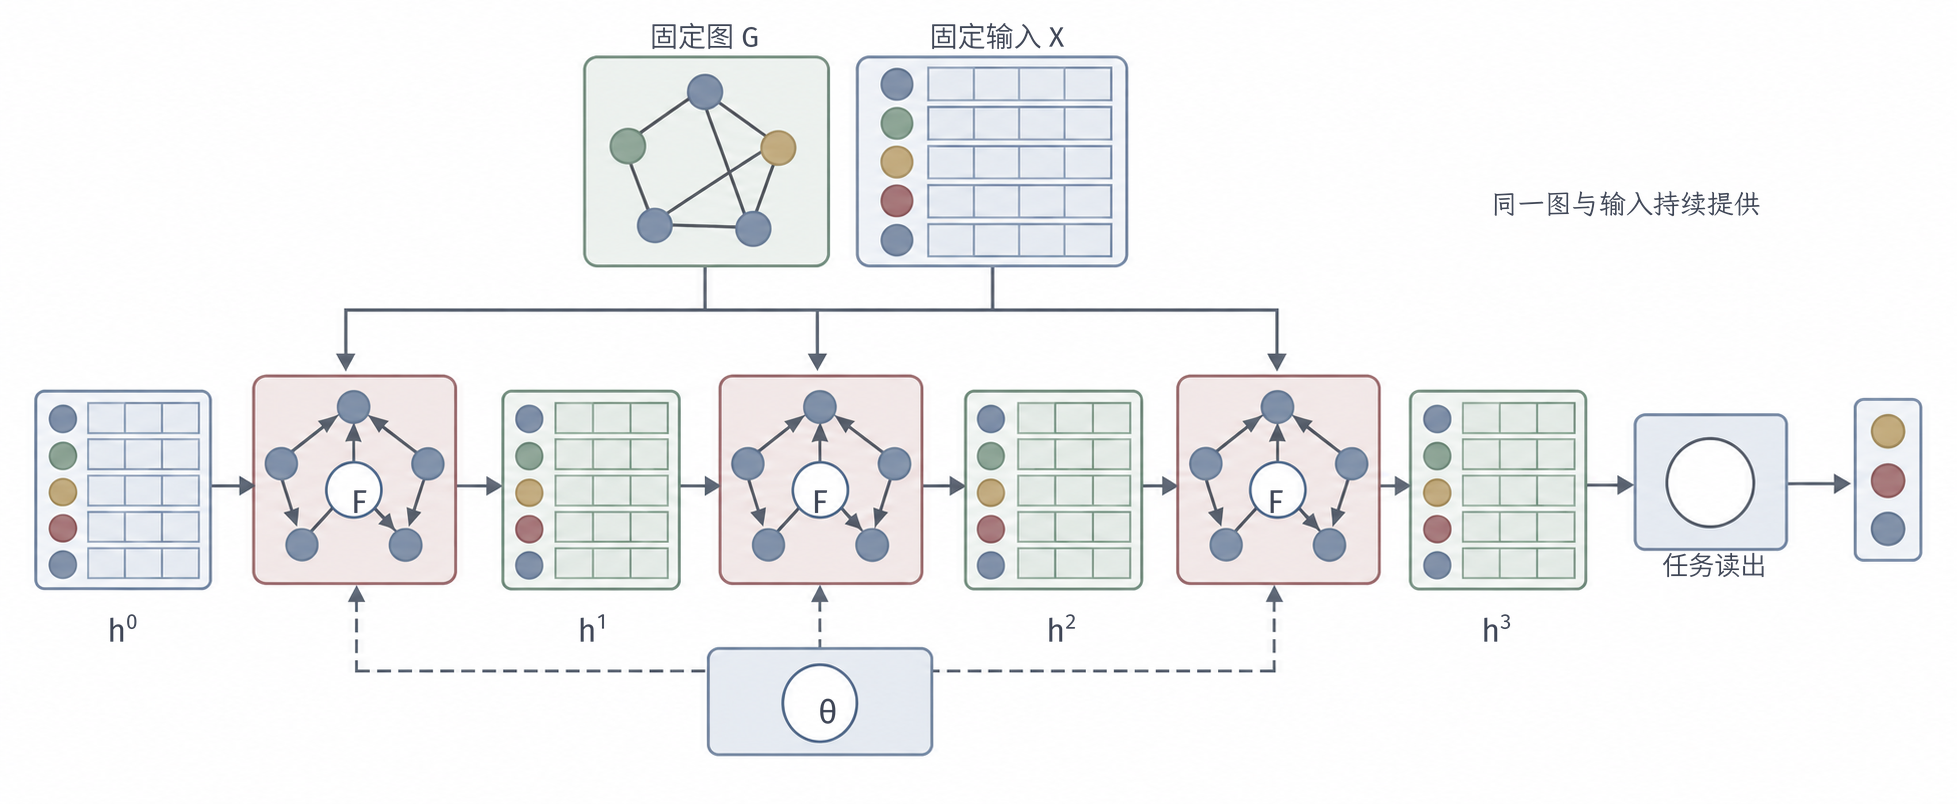
\includegraphics[width=165.693mm]{figures/05-neural-network-models/00-shared/generated/gnn-recurrent/figure.png}
  \caption{固定图上的循环更新。左侧表示邻接关系，右侧展开三轮共享更新$F_{\bm{\theta}}$，每个状态向量包含整张图的节点状态。固定图与输入特征在各轮重复供给，状态沿轮次传递，任务读出从最终状态形成预测。轮次是内部计算步，不表示图已经发生三个时间点的变化。}
  \label{fig:gnn-recurrent}
\end{figure*}
\FloatBarrier

共享参数使每轮复用同一规则，执行代价仍累加各轮计算。状态更新和任务监督决定传播内容；若目标是最短路或关系推理，还需检验这些表示与目标规则的对应。有限轮次模型与迭代至稳定的模型分别定义不同的输出。

\subsection{典型模型}
\label{sec:gnn-recurrent-models}

\subsubsection{以不动点为目标的图网络}
\label{sec:gnn-fixed-point-model}

早期GNN把目标状态定义为\term{不动点}（fixed point）：再次使用更新函数后仍不改变的状态，即$\bm{h}^*=F_{\bm{\theta}}(\bm{h}^*;\mathcal{G},\bm{X})$。它通过邻居状态迭代计算这一表示，再读取节点或图输出。为保证状态可确定，模型约束更新对状态具有收缩性；第~\ref{sec:gnn-state-convergence}节的状态收敛分析将给出条件及误差界。

这类模型的参数既影响输出映射，也影响不动点的位置。有限精度计算通常在相邻两轮差小于容差时停止，并设置最大轮数。达到轮数上限时输出当前近似状态，与容差已满足的情况分别记录。所需精度、迭代成本和收缩约束共同决定这一表示怎样求得。

\subsubsection{GGNN：固定轮次的门控传播}
\label{sec:gnn-ggnn}

如果任务只需要执行有限步，可以直接学习这些步骤的结果。\term{门控图神经网络}（gated graph neural network, GGNN）在聚合后用GRU式更新保留或写入状态。令$r(i,j)$表示边的类型与方向，邻域输入为
\begin{equation}
  \bm{a}_i^{(t)}=\sum_{j\in N(i)}\bm{W}_{r(i,j)}\bm{h}_j^{(t-1)}+\bm{b},
  \qquad
  \bm{h}_i^{(t)}=\operatorname{GRU}(\bm{h}_i^{(t-1)},\bm{a}_i^{(t)})\text{。}
  \label{eq:gnn-ggnn}
\end{equation}
这里$\bm{a}_i^{(t)}$是聚合输入向量，与边属性$\bm{a}_{i,j}$通过索引形式区分。原模型分别处理入边与出边并组合相应消息；式\eqref{eq:gnn-ggnn}写出一个统一的关系聚合形式，方向也可编码为不同类型\scite{li2016ggnn}

GRU的门机制沿用第~\ref{sec:rnn-gru}节。若把更新门解释为写入比例，状态可写为$\bm{h}_i^{(t)}=(\bm{1}-\bm{z}_i^{(t)})\odot\bm{h}_i^{(t-1)}+\bm{z}_i^{(t)}\odot\widetilde{\bm{h}}_i^{(t)}$；候选状态同时依赖聚合输入与经重置门处理的旧状态。门为节点提供选择性保留路径，远处证据则仍须沿边经过足够轮次。

GGNN用预先设定的$T$轮展开计算并训练，输出定义为第$T$轮状态，无需把它作为不动点近似。有限展开放宽了早期模型的收缩约束，状态行为由这些实际步骤决定。训练轮数是模型的一部分；预测时增加轮次就改变了所执行的函数，需要相应检验。

\subsection{参数学习}
\label{sec:gnn-recurrent-learning}

有限展开的梯度与随时间反向传播具有相同结构。设局部状态Jacobian矩阵$\bm{J}^{(t)}=\partial\bm{h}^{(t+1)}/\partial\bm{h}^{(t)}$，$\bm{\delta}^{(t)}$为第$t$轮状态的总梯度。若损失只读取末状态，则$\bm{\delta}^{(t)}=(\bm{J}^{(t)})^{\top}\bm{\delta}^{(t+1)}$；中间轮存在直接监督时，另加对应梯度。共享更新参数的梯度为
\begin{equation}
  \nabla_{\bm{\theta}}L
    =\left.\nabla_{\bm{\theta}}L\right|_{\mathrm{direct}}
      +\sum_{t=0}^{T-1}(\bm{B}^{(t)})^{\top}\bm{\delta}^{(t+1)}\text{，}
  \label{eq:gnn-recurrent-gradient}
\end{equation}
其中$\bm{B}^{(t)}=\partial F_{\bm{\theta}}(\bm{h}^{(t)};\mathcal{G},\bm{X})/\partial\bm{\theta}$固定当前输入状态求偏导。直接项包含读出参数等依赖；初态若依赖参数，还需计入初态梯度。截断展开会遗漏更早的间接贡献，降低存储与计算的同时改变所用梯度。

不动点模型还可用\term{隐式微分}（implicit differentiation）：对定义状态的方程求导，而不保存全部前向迭代。假设更新在不动点附近可微，令$\bm{J}_*=\partial F/\partial\bm{h}$、$\bm{B}_*=\partial F/\partial\bm{\theta}$在$\bm{h}^*$处取值。若$\bm{I}-\bm{J}_*$可逆，则
\begin{equation}
  (\bm{I}-\bm{J}_*)\frac{\partial\bm{h}^*}{\partial\bm{\theta}}
    =\bm{B}_*\text{。}
  \label{eq:gnn-implicit-state-gradient}
\end{equation}
这个等式来自对$\bm{h}^*=F_{\bm{\theta}}(\bm{h}^*)$两侧求导，并把状态导数项移到左侧。

实际需要的是标量损失的梯度。记$\bm{v}=\partial L/\partial\bm{h}^*\in\mathbb{R}^{nm}$为列向量，$\bm{D}_*=\partial\bm{h}^*/\partial\bm{\theta}\in\mathbb{R}^{nm\times p}$为状态对参数的导数矩阵。链式法则给出的状态间接项是$\bm{D}_*^{\top}\bm{v}$；若直接求出整个$\bm{D}_*$，就要为$p$个参数方向分别求状态响应。标量损失只需要这些响应在$\bm{v}$方向上的组合，因此可以先求一个$nm$维向量$\bm{u}$，再将它映回参数空间。具体地，解下面的转置线性方程，并用$\bm{B}_*^{\top}\bm{u}$计算间接项：
\begin{equation}
  (\bm{I}-\bm{J}_*^{\top})\bm{u}=\bm{v},\qquad
  \nabla_{\bm{\theta}}L
    =\left.\nabla_{\bm{\theta}}L\right|_{\mathrm{direct}}+\bm{B}_*^{\top}\bm{u}\text{。}
  \label{eq:gnn-implicit-loss-gradient}
\end{equation}
这一替换可以直接由两个线性关系核对。式\eqref{eq:gnn-implicit-state-gradient}给出$(\bm{I}-\bm{J}_*)\bm{D}_*=\bm{B}_*$，转置线性方程则给出$\bm{v}=(\bm{I}-\bm{J}_*)^{\top}\bm{u}$，所以
\[
  \begin{aligned}
    \bm{D}_*^{\top}\bm{v}
      &=\bm{D}_*^{\top}(\bm{I}-\bm{J}_*)^{\top}\bm{u}\\
      &=\bigl((\bm{I}-\bm{J}_*)\bm{D}_*\bigr)^{\top}\bm{u}
       =\bm{B}_*^{\top}\bm{u}\text{。}
  \end{aligned}
\]
直接项仍是在固定$\bm{h}^*$时，损失经读出等路径对参数产生的导数。这样只需解一个状态空间中的转置线性系统，无需形成整个状态导数矩阵。

无需显式求逆。若相应范数下$\lVert\bm{J}_*\rVert<1$，可用$\bm{u}^{(k+1)}=\bm{v}+\bm{J}_*^{\top}\bm{u}^{(k)}$迭代；Jacobian转置与向量的乘积由自动微分计算。前向状态与后向线性求解都有容差，两者都会影响最终梯度的精度。

对只迭代到近似状态的模型，有限展开给出实际执行步骤的梯度，隐式方法近似理想不动点目标的梯度，二者在尚未充分收敛时未必相同。停止条件、最大轮数和状态收缩速度因而既影响前向代价，也影响参数学习。

\section{图神经网络的扩展}
\label{sec:gnn-extensions}

前面的消息传递默认了几件事：所有边语义相同、图静止不变、一次关系只涉及两个节点、节点没有几何坐标。现实关系往往打破这些假设：论文之间“引用”和“合著”含义不同（多关系），社交网络随时变化（动态），一次合作涉及多人（高阶），分子中的原子还带三维坐标且预测要尊重旋转平移（几何）。扩展模型的共同原则是：把这些额外差异\emph{显式保留在输入里}，并设计相应的消息和对称约束，而不是让它们在无差别的聚合中被抹掉。

\subsection{多关系与异构图}
\label{sec:gnn-relational}

此前所有边都被当成同一种关系，但“甲引用乙”和“甲与乙合著”传递的是完全不同的信息，用同一套权重混合会把语义差别抹掉。\term{多关系图}（multi-relational graph）允许边带有类型，让不同类型的消息走不同的变换；\term{异构图}（heterogeneous graph）进一步允许节点本身分属不同类型（作者、论文）、具有不同属性和角色。节点类型与边类型是两个独立的分类维度，可以单独指定，也可以同时存在。

设关系类型集合为$R$，$N_r(i)$是通过类型$r$向$i$发送消息的邻居。\term{关系图卷积网络}（relational graph convolutional network, R-GCN）为每种关系使用一组独立变换：
\begin{equation}
  \bm{h}_i^{(l+1)}=\sigma\!\left(
    \bm{W}_0^{(l)}\bm{h}_i^{(l)}+
    \sum_{r\in R}\sum_{j\in N_r(i)}
      \frac{1}{c_{i,r}}\bm{W}_r^{(l)}\bm{h}_j^{(l)}\right)\text{。}
  \label{eq:gnn-rgcn}
\end{equation}
$c_{i,r}>0$是归一化系数，可在非空邻域取$|N_r(i)|$；空邻域的求和直接为零。$\bm{W}_0^{(l)}$负责自身状态，$\bm{W}_r^{(l)}$负责关系$r$。有向关系可增加单独的逆关系类型，使两个方向使用不同参数\scite{schlichtkrull2018rgcn}

关系数很大时，每种关系独立学习一个稠密矩阵会增加参数与数据需求。可以用基分解$\bm{W}_r=\sum_{b=1}^{B}a_{r,b}\bm{V}_b$，让各关系共享$B$个基础矩阵，只学习不同系数。固定输入输出宽度$m$时，参数量由$|R|m^2$改为$Bm^2+|R|B$，代价是关系变换被限制在同一矩阵子空间。

不同节点类型的原始特征维度可能不同，可以先用类型相关的输入映射投到公共空间，再按关系传递。聚合还可先在每种关系内部组合，再学习关系间权重。置换等变性在重编号后仍成立，但类型也须跟着节点与边重排。作者和论文的属性角色保持各自含义，重编号只改变保存它们的位置。

图~\ref{fig:gnn-typed-relations}用作者与论文两类节点说明这种分工。类型映射先对齐特征空间，关系变换与归一化随后保留“撰写”和“引用”的区别，自身状态仍有独立路径。

\begin{figure*}[htbp]
  \centering
  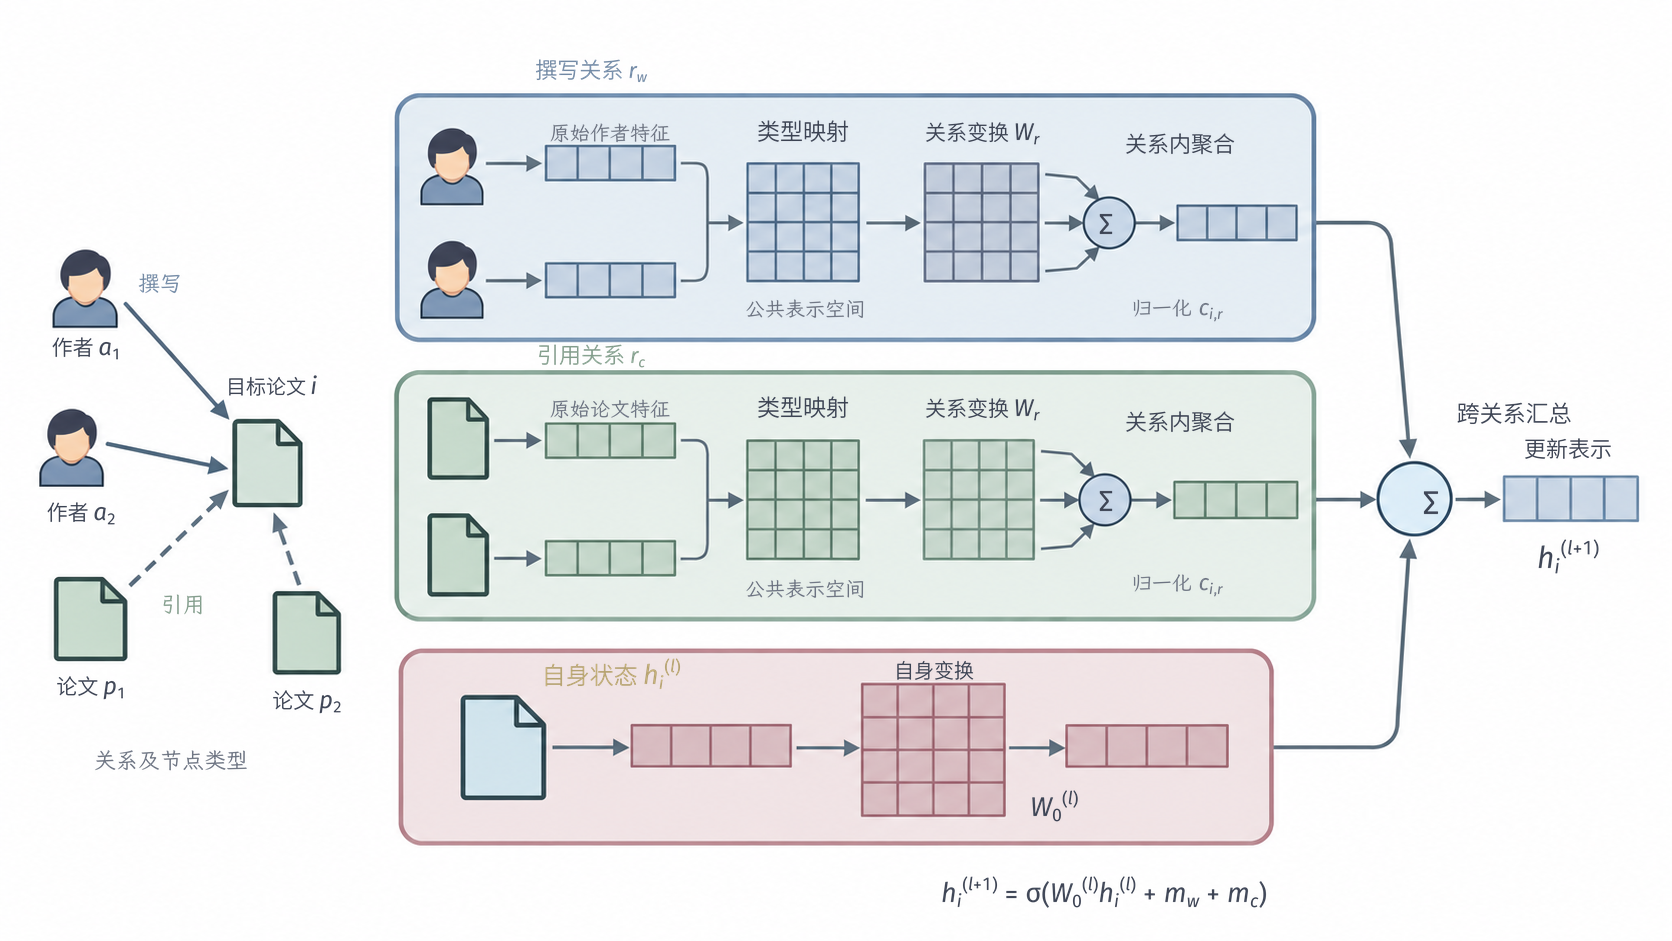
\includegraphics[width=141.563mm]{figures/05-neural-network-models/00-shared/generated/gnn-typed-relations/figure.png}
  \caption{两类节点与两种关系的消息组织。作者的撰写关系和论文的引用关系分别经过类型映射与关系变换，再在各关系内部归一化聚合；两路结果$\bm m_{\mathrm w}$、$\bm m_{\mathrm c}$与独立的自身状态路径汇总，形成目标论文的新表示。各类型的特征组表示同类节点，不表示提前求和；矩阵网格只示意变换，不声明实际维度。}
  \label{fig:gnn-typed-relations}
\end{figure*}
\FloatBarrier

\subsection{动态图}
\label{sec:gnn-dynamic}

社交互动、交易、设备连接都会随时间出现和消失，这时“固定图上传播十轮”和“现实中十个不同时刻”是两回事：前者是对\emph{同一个输入}做十次内部计算，后者是\emph{十份不同的输入图}。\term{动态图}（dynamic graph）把节点、边或属性随时间的变化也作为输入，模型既要处理当前关系，又要明确在做某个预测时哪些历史是合法可见的（不能用未来的边预测现在）。一种表示是\term{图快照}（graph snapshot）：在时刻$t$取得$\mathcal{G}_t$与$\bm{X}_t$，先在每张快照内用GNN编码当前邻域，再用循环状态沿时间累积。对持续存在的节点可写为
\begin{equation}
  \bm{z}_{i,t}=\operatorname{GNN}(\mathcal{G}_t,\bm{X}_t)_i,
  \qquad
  \bm{s}_{i,t}=\operatorname{GRU}(\bm{s}_{i,t-1},\bm{z}_{i,t})\text{。}
  \label{eq:gnn-snapshot-dynamics}
\end{equation}
这里$\bm{z}_{i,t}$包含当前图中的邻域信息，$\bm{s}_{i,t}$维护跨时间历史。节点身份用于对齐相邻快照中的同一个对象；新节点的初态、节点消失后的状态保留与重现规则也要约定。快照间隔决定哪些短时事件被合并或遗漏。

另一种表示是带时间戳的\term{事件序列}（event sequence），例如第$q$个事件$(i_q,j_q,\tau_q,\bm{a}_q)$表示两个节点在时刻$\tau_q$发生互动。每个节点维护自己的记忆，在事件发生后更新相关状态。消息可以读取两端的事件前记忆、事件属性，以及距离该节点上次更新的时间间隔；不参与事件的节点记忆可以暂时保留。TGN以消息函数、消息聚合、记忆更新和时序表示等模块组织这一类计算\scite{rossi2020tgn}

预测互动是否发生时，应先用事件发生前的历史评分，再用实际发生的事件更新记忆。这样的先后顺序使评分只读取当时的历史，随后到达的事件再进入记忆。批量事件处理也要明确是否能读取同批中较早的事件；同一时刻事件的处理应采用约定的同时更新或已有先后关系，使事件次序对应实际观测含义。

图~\ref{fig:gnn-dynamic-before-update}把内部传播、观测时间与事件先后三种顺序分开。下半部的评分位于消息和记忆更新之前，正是避免把待预测事件提前写入历史的关键。

\begin{figure*}[htbp]
  \centering
  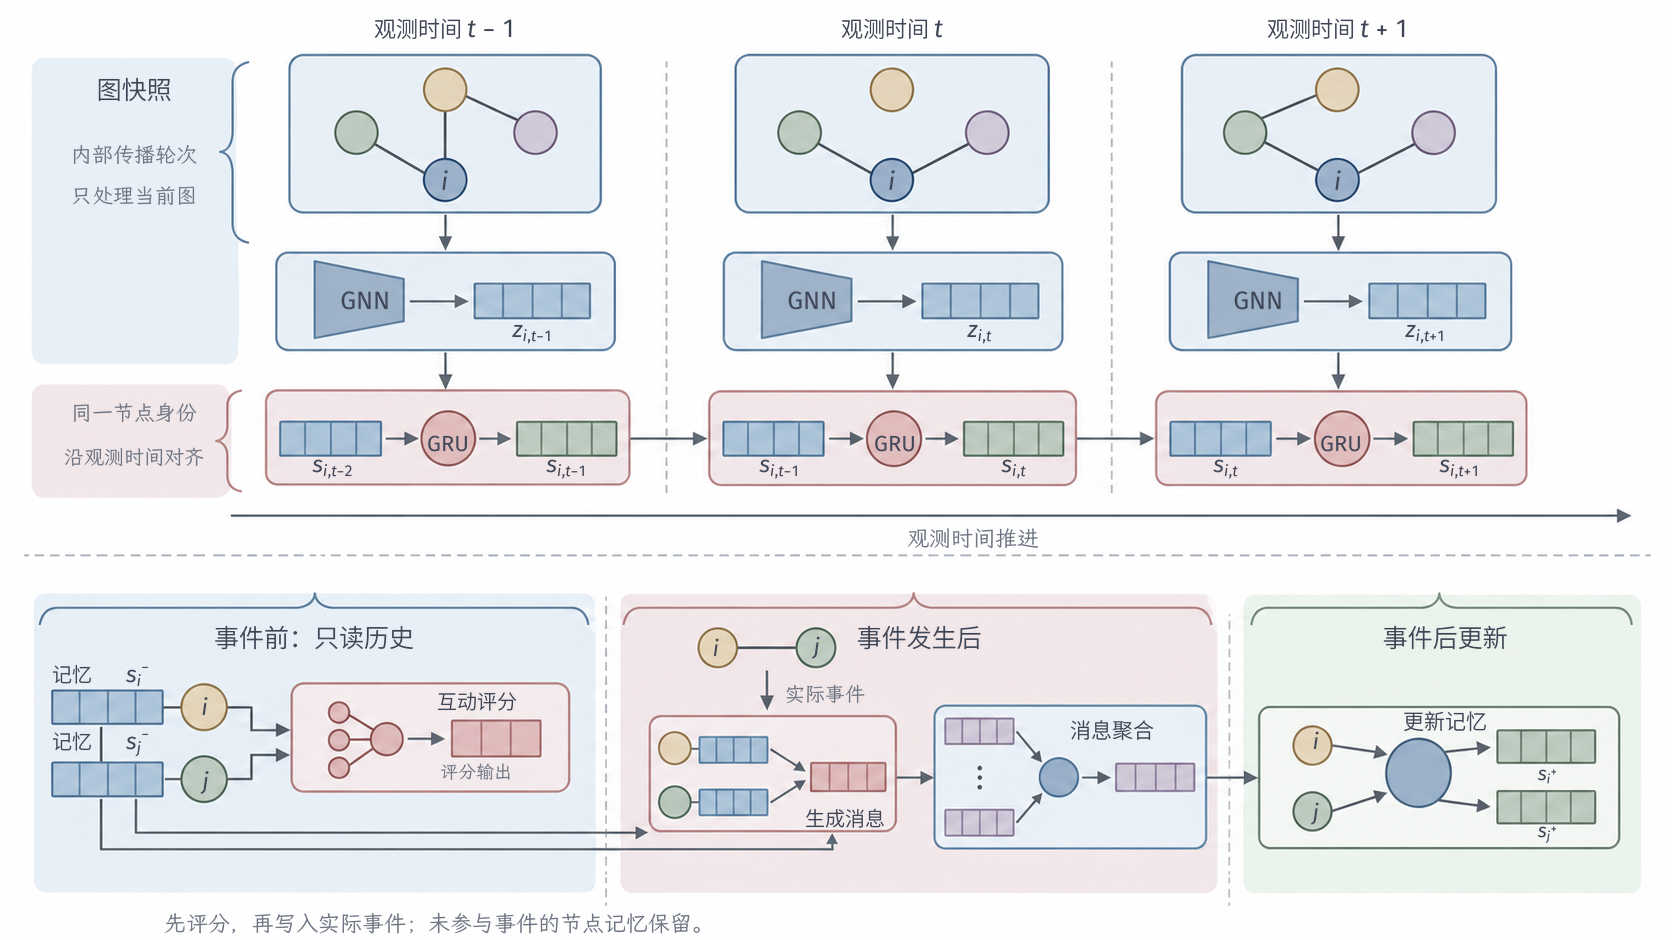
\includegraphics[width=141.563mm]{figures/05-neural-network-models/00-shared/generated/gnn-dynamic-before-update/figure.png}
  \caption{动态图的两种时间组织。上半部区分固定快照中的内部传播与同一节点沿观测时间的GRU状态演化；下半部先用事件前记忆评分，实际事件到达后才生成消息、聚合并更新参与节点。未参与事件的节点保留记忆。}
  \label{fig:gnn-dynamic-before-update}
\end{figure*}
\FloatBarrier

训练时可沿快照或事件展开反向传播，并在长流中按需要截断。评估未来事件时按时间划分，状态只由约定的可见历史推进；评估新节点时还要额外检查训练阶段是否已经接触其信息。内部传播深度、历史记忆长度和观测时间间隔共同影响计算，但衡量的是三种不同范围。

\subsection{高阶关系}
\label{sec:gnn-higher-order}

普通图的一条边只能连接两个节点，但现实中常有“一件事同时涉及多个对象”：一次三人合著、一笔多方交易、一个化学反应中多个反应物共同参与。如果把这样一个$k$元关系硬拆成所有两两配对的边，就无法区分“一次三人合作”与“三次各自的两人合作”——拆成的成对边集合可能完全相同。\term{超图}（hypergraph）用\term{超边}（hyperedge）直接表示一次连接多个节点的关系，把完整的参与组保留下来。记$\mathcal{H}=(V,\mathcal{E})$，其中$\mathcal{E}$是节点子集的集合；一条超边$S_a\subseteq V$就保留这次关系的完整参与组。

图~\ref{fig:gnn-hyperedge}展示一种计算表示：先让节点向超边聚合，再让超边把结果传回参与节点。将每条超边作为额外对象，会得到节点与关系对象构成的二部图；超边属性及非线性变换可以放在中间状态上。
\begin{figure*}[htb]
  \centering
  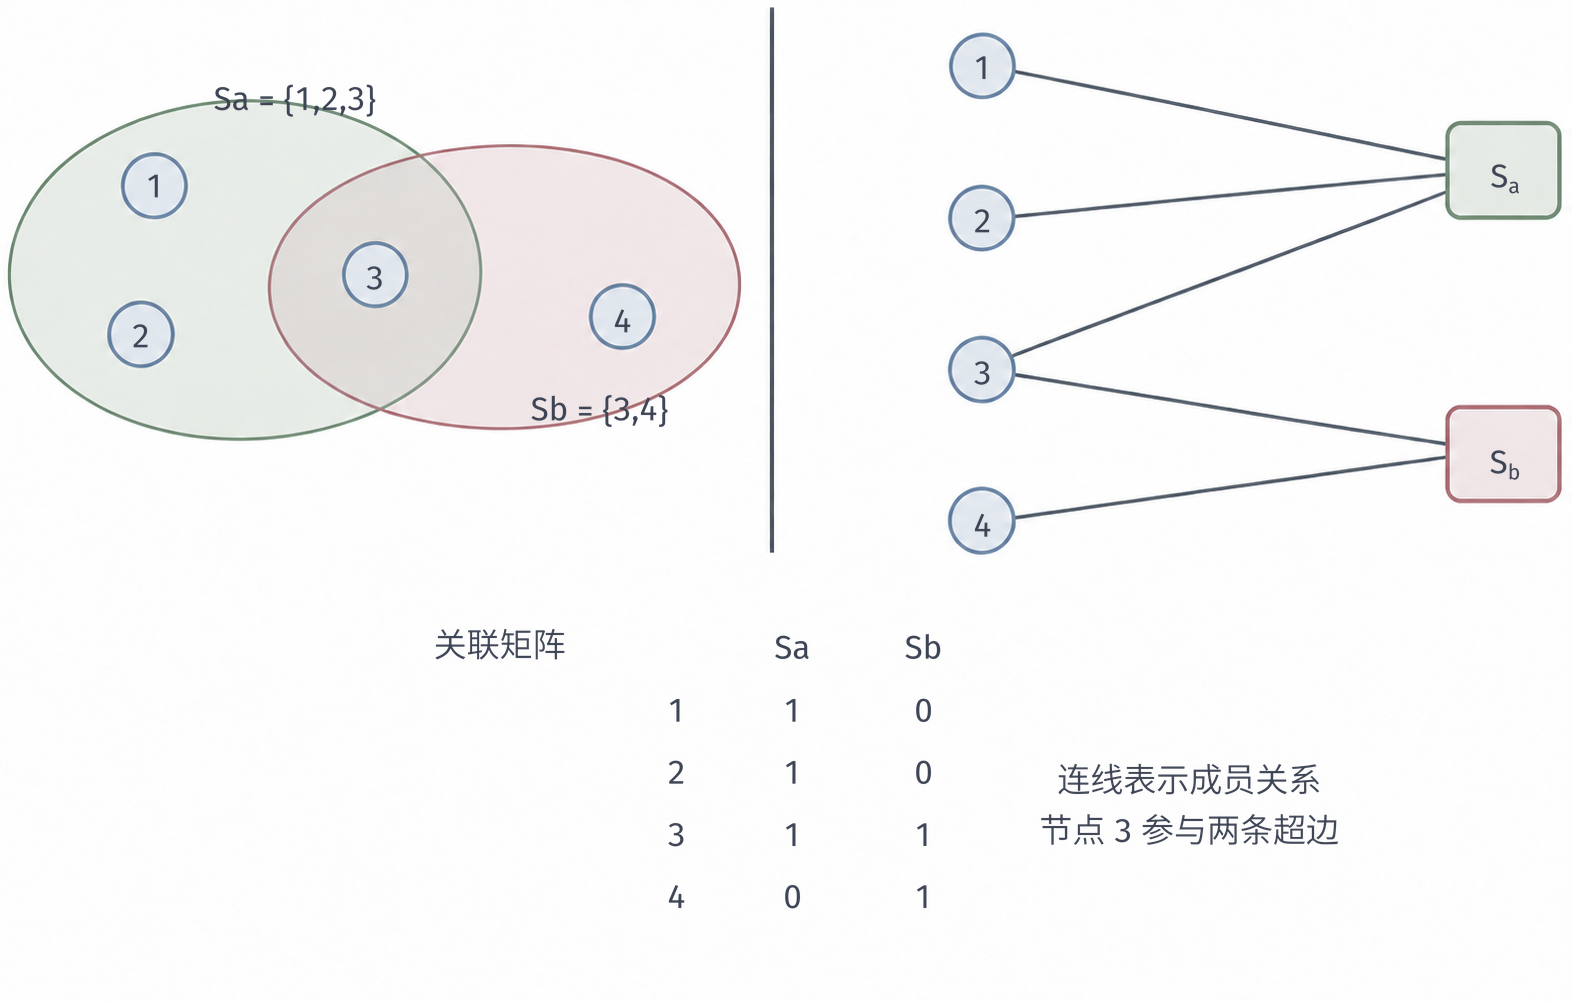
\includegraphics[width=133.096mm]{figures/05-neural-network-models/00-shared/generated/gnn-hyperedge/figure.png}
  \caption{超边及其关联表示。左侧一条超边$S_a$连接节点1、2、3，另一条超边$S_b$连接节点3、4。右侧将超边画成方框，以连线表示参与关系；下方$4\times2$关联矩阵用同一组0／1关系把“集合、二部图、矩阵”对应起来。方框保存关系状态，原始参与者仍由圆形节点表示。}
  \label{fig:gnn-hyperedge}
\end{figure*}
\FloatBarrier

令\term{关联矩阵}（incidence matrix）$\bm{B}\in\{0,1\}^{n\times h}$记录节点是否属于超边，$h=|\mathcal{E}|$，$\bm{B}_{i,a}=1$表示$i\in S_a$。设超边权重为$w_a>0$，$\bm{W}_e=\operatorname{diag}(w_1,\ldots,w_h)$，节点度$d_i=\sum_a\bm{B}_{i,a}w_a$，超边大小$s_a=\sum_i\bm{B}_{i,a}$。对非空超边及非孤立节点，一个归一化的传播为
\begin{equation}
  \bm{H}'=\sigma\!\left(
    \bm{D}_v^{-1/2}\bm{B}\bm{W}_e\bm{D}_e^{-1}
      \bm{B}^{\top}\bm{D}_v^{-1/2}\bm{H}\bm{\Theta}\right)\text{，}
  \label{eq:gnn-hypergraph-layer}
\end{equation}
其中$\bm{D}_v=\operatorname{diag}(d_i)$、$\bm{D}_e=\operatorname{diag}(s_a)$，$\bm{\Theta}$是特征变换矩阵。HGNN采用了这一类归一化超图卷积\scite{feng2019hgnn}

从右向左看，先由$\bm{H}\bm{\Theta}$变换节点特征，右端$\bm{D}_v^{-1/2}$再把发送节点$j$的表示除以$\sqrt{d_j}$。$\bm{B}^{\top}$将这些表示汇总到各条超边，$\bm{D}_e^{-1}$除以超边大小$s_a$，得到参与节点预缩放表示的平均值。随后$\bm{W}_e$把第$a$条超边的平均值乘以$w_a$，$\bm{B}$将这个结果送回该超边的全部参与节点，并把同一节点收到的各条超边结果相加。最左侧$\bm{D}_v^{-1/2}$再把接收节点$i$的结果除以$\sqrt{d_i}$，最后才施加激活。

因此，在激活之前，发送节点$j$的变换后表示$(\bm{H}\bm{\Theta})_{j,:}$对接收节点$i$的总传播系数为
\[
  \sum_{a:\,i,j\in S_a}\frac{w_a}{s_a\sqrt{d_i d_j}}\text{。}
\]
求和遍历同时包含$i$与$j$的超边；同一节点也会经其所属超边收到自身的贡献。这里按$s_a$求的是预缩放表示的组内平均，两端的节点度还会调整发送与接收尺度，整个节点传播不必是原始表示的简单平均。

我们可以沿图~\ref{fig:gnn-hyperedge}复核一次传播。取$S_a=\{1,2,3\}$、$S_b=\{3,4\}$，两条超边的权重均为$1$；作为教学算例，令单通道输入$\bm{H}=(1,2,3,4)^{\top}$、$\bm{\Theta}=1$，并使用恒等激活。节点度为$(1,1,2,1)$，超边大小为$(3,2)$。发送端预缩放后，四个节点的值为$(1,2,3/\sqrt{2},4)$；两条超边分别得到平均值$(1+2+3/\sqrt{2})/3$与$(3/\sqrt{2}+4)/2$。超边权重都为$1$，因此这两个平均值保持原值送回。节点3参与两条超边，将两个结果相加，再除以自身的$\sqrt{d_3}=\sqrt{2}$，得到
\[
  \bm{H}'_{3,1}
    =\frac{1}{\sqrt{2}}\left(
       \frac{1+2+3/\sqrt{2}}{3}
       +\frac{3/\sqrt{2}+4}{2}\right)
    =\frac{3}{\sqrt{2}}+\frac{5}{4}\text{。}
\]
这个结果把超边内平均、超边间累加和接收端缩放对应到同一次传播。

记录完整参与组后，还需要检查计算是否保留了这些组的差别。上述线性传播可以合成一个节点间矩阵（式\eqref{eq:gnn-hypergraph-layer}）。若两张超图产生相同矩阵，这一层也不能保留它们不同的组关系。任务依赖具体组时，可以在合成节点传播矩阵前保留超边状态、属性或组内非线性，使组关系继续进入输出。

另一类\term{高阶图网络}（higher-order graph neural network）把节点组作为状态对象，例如为节点对维护$\bm{h}_{i,j}$，使网络能够组合单节点状态难以保留的关系。它通过节点组索引安排状态与交互，可以由原图构造这些组，也可以读取已知高阶关系。Morris等将这种思路与高阶WL方法联系起来\scite{morris2019higherorder} 若显式维护所有$k$元节点组，状态数可达$O(n^k)$；选取部分子结构或局部组可以降低代价，但相应的区分能力也要重新说明。

\subsection{几何关系与对称性约束}
\label{sec:gnn-geometric}

在分子、点云这类数据中，节点除了连接关系还带有三维坐标。这里有一个比编号无关更严格的对称要求：把整个分子平移一下或在空间中转个方向，它的能量、毒性等\emph{标量性质}不应改变；而预测出的力、位移等\emph{向量}则应当跟着坐标系一起旋转。如果把绝对坐标直接喂给普通消息函数，网络就可能依赖“分子在空间中的绝对朝向”这种人为选择，违背物理对称性。几何图网络的做法是只在消息中使用\emph{旋转平移下不变的量}（如原子间距），需要输出向量时再乘以\emph{等变的相对方向}。

令变换后的输入坐标为$\bar{\bm{r}}_i=\bm{Q}\bm{r}_i+\bm{t}$，其中$\bm{t}\in\mathbb{R}^{3}$是平移，正交矩阵$\bm{Q}$满足$\bm{Q}^{\top}\bm{Q}=\bm{I}_3$。相对位移满足$\bar{\bm{r}}_i-\bar{\bm{r}}_j=\bm{Q}(\bm{r}_i-\bm{r}_j)$，距离$\lVert\bm{r}_i-\bm{r}_j\rVert_2$保持不变。用距离和其他不变属性产生标量消息，再用标量系数乘相对位移，就能构造等变的坐标更新。下面的撇号表示网络层的输出，因而$\bm{r}'_i$与变换后的输入$\bar{\bm{r}}_i$表示两种操作的结果。一个EGNN式的层可写为
\begin{equation}
  \begin{aligned}
    \bm{m}_{i\leftarrow j}
      &=\phi_e(\bm{h}_i,\bm{h}_j,
        \lVert\bm{r}_i-\bm{r}_j\rVert_2^2,\bm{a}_{i,j}),\\
    \bm{r}'_i&=\bm{r}_i+
      c_i\sum_{j\in N(i)}(\bm{r}_i-\bm{r}_j)\phi_r(\bm{m}_{i\leftarrow j}),\\
    \bm{h}'_i&=\phi_h\!\left(\bm{h}_i,\sum_{j\in N(i)}\bm{m}_{i\leftarrow j}\right)\text{。}
  \end{aligned}
  \label{eq:gnn-egnn}
\end{equation}
$\phi_r$输出标量，$c_i$是与坐标变换无关的归一化系数，$\bm{h}_i$此处由对所选欧氏变换不变的标量通道组成，边属性也具有相同不变性。EGNN使用距离构造消息，并用这种相对位移加权实现欧氏变换等变性\scite{satorras2021egnn}

证明只需跟踪各对象的变化。记$\bm{r}=(\bm{r}_j)_{j\in V}$为全部节点的坐标，$\bm{Q}\bm{r}+\bm{t}$表示对每个节点施加同一变换。以$\Psi$表示式\eqref{eq:gnn-egnn}中的坐标更新，把原输入的层输出记为$\bm{r}'_i=\Psi(\bm{r})_i$，把变换输入的层输出记为$\bar{\bm{r}}'_i=\Psi(\bar{\bm{r}})_i$；不变的节点特征、边属性和相应邻域暂时省略在$\Psi$的记号中。距离不变，所以消息及$\phi_r$不变；相对位移变为$\bm{Q}(\bm{r}_i-\bm{r}_j)$，整段坐标增量随$\bm{Q}$变换，加回$\bar{\bm{r}}_i=\bm{Q}\bm{r}_i+\bm{t}$后便有
\[
  \bar{\bm{r}}'_i
    =\Psi(\bm{Q}\bm{r}+\bm{t})_i
    =\bm{Q}\Psi(\bm{r})_i+\bm{t}
    =\bm{Q}\bm{r}'_i+\bm{t}\text{。}
\]
左侧先变换输入再执行层更新，右侧先对原输入执行层更新再变换输出，两种计算顺序得到相同坐标。变换输入后的标量层输出同时满足$\bar{\bm{h}}'_i=\bm{h}'_i$。邻接构造也须遵守该对称性，使整体变换前后的邻域对应，例如按距离阈值建边；若按固定坐标轴上的绝对位置选边，消息函数对称仍不足以保证整个模型对称。

正交矩阵还包括镜像反射。距离不变的模型因此可能无法区分互为镜像的手性构型；若目标会因镜像而改变，就需要只约束适用的对称群，并引入能保留相应方向关系的信息。所选对称群由目标决定：任务需要区分的方向关系应保留在输入与消息中。

若标量能量预测$\widehat E$可微且具有相应不变性，定义$\widehat{\bm{f}}_i=-\nabla_{\bm{r}_i}\widehat E$可以得到随旋转等变的力预测。具体地，由$\widehat E(\bar{\bm{r}})=\widehat E(\bm{r})$和链式法则，有$\bm{Q}^{\top}\nabla_{\bar{\bm{r}}_i}\widehat E(\bar{\bm{r}})=\nabla_{\bm{r}_i}\widehat E(\bm{r})$；$\bm{Q}$正交，故$\widehat{\bm{f}}_i(\bar{\bm{r}})=\bm{Q}\widehat{\bm{f}}_i(\bm{r})$。能量与力由同一可微函数联系，具有相应数学一致性；预测精度再由监督、构型覆盖和数值计算检验。

\section{理论分析}
\label{sec:gnn-theory}

与前几章一样，本节严格区分三个层面的问题：\emph{表达能力}问消息传递的结构是否\textbf{允许}网络区分目标所需的不同图（哪些信息在聚合中被不可逆地抹掉）；\emph{收敛性}有两个不同对象——参数能否被梯度下降\textbf{优化}到驻点，以及循环图网络反复迭代后状态能否\textbf{收敛}到唯一不动点；\emph{泛化性}问在\emph{独立的整图样本}上学到的规则对新图的风险。图结构既是帮助（强对称约束压缩了假设空间），也可能是限制（删掉了某些区分能力），下面保留结构区分能力、状态求值和样本边界的分析。

\subsection{表达能力}
\label{sec:gnn-expressivity}
\label{sec:gnn-propagation-theory}

表达能力问题在图上有一个特别干净的判别准则，可以一直追溯到消息传递的定义：\emph{如果两个节点（或两张图）在每一轮聚合后都得到完全相同的表示，那么任何只读取这些表示的读出都永远无法区分它们}。因此，要判断一个图网络能表达什么，只需检查在给定初始特征、聚合方式和传播轮次下，哪些不同结构会被“撞”成相同的表示。这里有两个层面的信息损失要分清：一是\emph{聚合函数}本身是否保留邻居的多重集（数量、内容），二是\emph{传播轮次和读出}是否保留了目标所需的结构关系。聚合若保留多重集、轮次足够、读出也保留所需结构，表达能力才可能达标；GIN正是通过把聚合和更新都设计成单射来逼近这条上界\scite{xu2019gin}。

\begin{theorem}[求和消息传递对度目标的表达与连通性目标的限制]
\label{thm:gnn-degree-connectivity-expression}
设节点初始特征均为$1$，图为无向简单图，最大度不超过预先固定的整数$D$。
允许保留邻居求和结果并接ReLU前馈读出，则一轮消息传递即可准确表示任意给定的节点度函数$g(\deg v)$。
但若各层只用共享节点更新和邻居多重集聚合，整图读出只使用最终节点表示的多重集，不加入节点标识或其他结构特征，则任何层数都无法区分六节点环$C_6$和两个不相交的三节点环$C_3\sqcup C_3$。对在两张图上分别取$1$与$0$的连通性目标，任意标量候选至少在一张图上有$1/2$的绝对逼近误差。
\end{theorem}
\begin{proof}
邻居特征求和恰等于度数。对有限整数$0,\ldots,D$指定$g$的值，分段线性插值可由ReLU读出准确表示。
两张环图则都有六个节点，每个节点有两个邻居。从相同初始特征出发，各轮节点都收到由两个相同向量组成的多重集，所以两张图的全部节点始终得到同一表示。整图读出相同，其输出不能同时距$0$和$1$小于$1/2$。
\end{proof}
求和能够保留数量信息，平均聚合在常数特征上却把不同度数都映为$1$。这解释了为何聚合方式直接影响候选空间。更强的GIN区分结论以单射更新与读出为条件，仍受相应图对的可区分性限制\scite{xu2019gin} 连通性反例针对上述消息传递族，并不覆盖加入高阶关系或结构位置特征的扩展。

\paragraph{反复传播对目标信息的影响：过平滑。}
\label{sec:gnn-oversmoothing}

多轮传播能扩大感受野，但直觉上也能想到它的副作用：如果每一轮都把节点的表示与邻居平均，那么传播很多轮之后，互相连通的所有节点都会被“搅”成越来越接近的同一个表示，节点自身的身份差异被逐渐抹掉。\term{过平滑}（oversmoothing）指的就是这种\emph{随深度增加、与区分节点有关的信息不断衰减}的现象；它不要求所有坐标严格相等才发生——只要任务所需的差异在各坐标尚未完全相等时就已经被削弱到无法利用，分类就会受损。值得注意的是，即便不同层使用不同参数，这种反复混合仍可能发生。

\begin{figure}[htbp]
  \centering
  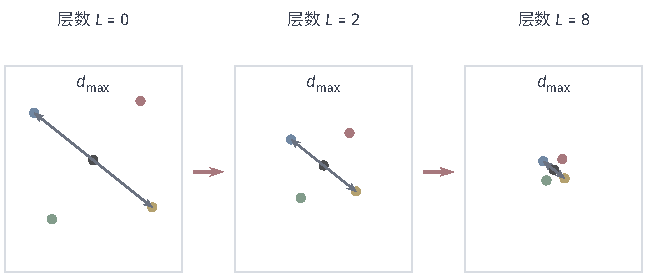
\includegraphics[width=109.580mm]{figures/05-neural-network-models/00-shared/tikz/gnn-oversmoothing/figure.pdf}
  \caption{过平滑的二维投影示意。五种颜色始终代表同五个节点，位置只是人为构造的表示投影，并非t-SNE实验；随着传播层数增加，点间最大距离缩小，节点身份仍在但可供下游区分的表示差异逐渐消失。过平滑描述的是任务相关差异受损，不要求所有坐标严格相等。}
  \label{fig:gnn-oversmoothing}
\end{figure}
\FloatBarrier

先看一个能够精确求解的简化模型：令激活与通道变换都为恒等，只反复计算$\bm{H}^{(l+1)}=\bm{S}\bm{H}^{(l)}$。假定非负无向图连通，并在每个节点加入正自环；对应$\bm{S}$具有唯一特征值1，其余特征值的绝对值小于1。定义单位向量
\[
  q_i=\frac{\sqrt{\widetilde d_i}}{\sqrt{\sum_j\widetilde d_j}}\text{，}
\]
则特征分解给出
\begin{equation}
  \bm{S}^L\bm{X}\longrightarrow\bm{q}\bm{q}^{\top}\bm{X},\qquad
  \lVert\bm{S}^L\bm{X}-\bm{q}\bm{q}^{\top}\bm{X}\rVert_F
    \leq\rho^L\lVert\bm{X}\rVert_F\text{，}
  \label{eq:gnn-linear-oversmoothing}
\end{equation}
其中$\rho$是其他特征值绝对值的最大值。证明依据是$\bm{q}$方向保持不变，其正交方向每次乘以绝对值至多为$\rho$的特征值。若图只有一个节点，就没有其他谱模式；此时约定$\rho=0$，从第一轮起传播结果已经等于$\bm q\bm q^{\top}\bm X$，式\eqref{eq:gnn-linear-oversmoothing}中$L\geq1$时的误差为零。

极限中，每个节点只剩同一个特征向量的度相关倍数；除以$\sqrt{\widetilde d_i}$后便相同。若图不连通，每个连通分量保留一个相应方向；若没有破除周期的条件，例如无自环的二部图，状态还可能振荡。这里的极限与速度由连通性、归一化和破除周期的自环条件共同支持。

真实GCN的非线性、学习权重及跨层连接会改变这一纯线性传播，式\eqref{eq:gnn-linear-oversmoothing}先说明反复混合的基本机制。Oono与Suzuki在特定激活及参数范数条件下进一步分析了表示靠近低维子空间的速度，说明传播谱与权重尺度需要联合考察\scite{oono2020oversmoothing} 低频聚合在有限深度可能有用，任务需要保留的差异被过度削弱时才构成问题。

残差连接可以为旧表示保留额外路径，跨层拼接或读出可以直接读取较浅表示，初始特征注入则持续补充原始节点差异。这些设计改变了反复纯混合的形式。若恒等分支加入后又与传播共同归一化，表示仍可能持续混合；残差实际保留多少差异，取决于完整更新。

\paragraph{窄通路对查询目标的限制：过压缩。}
\label{sec:gnn-oversquashing}

过平滑是“大家变得一样”，另一种困难则不同：远处\emph{确实有大量不同信息}要传过来，但通往当前节点的“通路太窄”，这些信息在瓶颈处被过度压缩、互相干扰，单个远处对象的影响被稀释到几乎无法辨识。\term{过压缩}（oversquashing）指大量关系信息沿有限条路径汇入有限维状态时，任务所需的远处影响难以有效传递。它关注的是远期影响\emph{通过哪些通路、汇入多大的状态}，Alon与Yahav从这一信息瓶颈出发分析了长程图任务\scite{alon2021oversquashing}。注意它与过平滑的判别方式不同：过压缩中各节点的表示并不一定趋于相同，真正的问题是单一输出对某个具体远端输入的敏感度趋近于零。

一个二叉树例子能展示具体机制。设每个内部节点只把两个子节点的标量取平均，深度为$k$的$2^k$个叶子为$x_j$，则根状态为$h_{\mathrm{root}}=2^{-k}\sum_jx_j$，根对单个叶子的偏导为$2^{-k}$。距离每增加一层，每个叶子的单独影响就减半，$k$层后衰减为$2^{-k}$；但根与各叶状态始终不同，所以这不是过平滑。图~\ref{fig:gnn-bottleneck}把汇聚树与图中“两组节点只能通过一条桥边通信”的情形对应起来。

\begin{figure*}[htb]
  \centering
  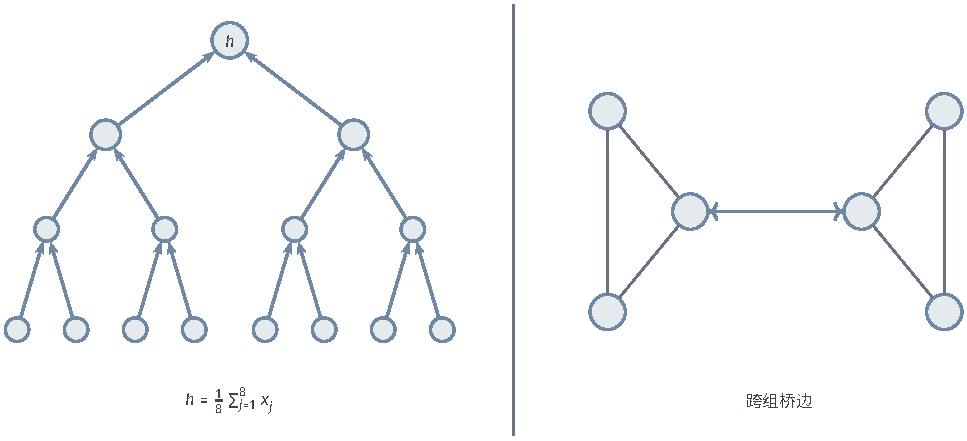
\includegraphics[width=163.791mm]{figures/05-neural-network-models/00-shared/tikz/gnn-bottleneck/figure.pdf}
  \caption{两种信息汇聚瓶颈。左侧八个叶子经三层平均进入一个根状态，每个叶子的影响系数为$1/8$；右侧两组节点的跨组信息必须经过一条桥边。图不要求所有状态相同，强调的是大量信息必须经过较少的表示通路。}
  \label{fig:gnn-bottleneck}
\end{figure*}
\FloatBarrier

若目标恰是叶子的平均，这种压缩就是所需计算；若目标要根据查询分别检索某个叶子，单一平均已经丢掉必要差别。因此，过压缩要相对于任务解释。压缩容量的分析需同时规定精度、噪声或连续性条件；无限精度实数与设备上的有限精度状态能够区分的历史数目不同。

增加状态宽度可以提供更多通道，增加传播轮次可以到达更远处，却也可能增加汇入同一状态的信息量。修改图结构、加入长程连接或全局读取，可以缩短路径并扩大跨区域通路；这些做法也改变了关系假设和计算量。残差主要保留已有信息路径，未必能解除一条桥边上的瓶颈。状态收敛、过平滑与过压缩因而需要分别诊断，再选择对应设计。


\subsection{循环状态的收敛}
\label{sec:gnn-convergence}

参数学习与状态求值是两个不同过程。有限轮消息传递直接定义输出，参数优化沿用第\ref{sec:ffn-convergence}节的相应条件；循环图网络若以不动点定义预测，则还需保证固定图、输入和参数下的状态迭代能够得到确定结果。


\label{sec:gnn-state-convergence}

不动点模型若迭代振荡或发散，就无法由极限确定预测。\term{压缩映射}（contraction mapping）给出充分条件：对同一输入，无论从哪两个初始状态出发，经过一次更新后它们之间的距离都按某个严格小于1的比例$c$缩小；在状态域完整且更新不离开该域时，反复迭代便趋向同一状态。这里的距离针对整张图的状态向量，消息聚合和所有节点的更新共同决定这个比例。

\begin{theorem}[收缩循环图网络的状态解唯一性与收敛速度]
\label{thm:gnn-state-solution}
固定图、输入与参数，若更新把非空闭状态域映回自身，并在同一范数下以非负统一比例$c<1$收缩，则任意该域内初态都趋于唯一状态$\bm h^*$，且
\begin{equation}
 \lVert\bm h^{(t)}-\bm h^*\rVert\leq c^t\lVert\bm h^{(0)}-\bm h^*\rVert\text{。}
 \label{eq:gnn-contraction-error}
\end{equation}
\end{theorem}
这给出了状态存在、唯一和迭代误差的结论；所用压缩映射结论可参考\BookChapterRef{chap:mathematical-analysis}{卷1《数学准备：计算、分析与几何》的“测度与分析”章}。

在同一收缩条件下，相邻状态差还给出可检查的后验误差证书：对$t\geq1$，$\lVert\bm{h}^{(t)}-\bm{h}^*\rVert\leq c(1-c)^{-1}\lVert\bm{h}^{(t)}-\bm{h}^{(t-1)}\rVert$。$c$接近1时，误差证书中的放大系数较大，同一相邻差对应较宽的最终误差上界；迭代速度与停止容差由此联系起来。

例如采用矩阵状态更新$\bm{H}'=\sigma(\bm{S}\bm{H}\bm{W}+\bm{B}_x)$，其中$\bm{B}_x\in\mathbb{R}^{n\times m}$为固定输入项。若$\sigma$是$L_\sigma$-Lipschitz的，则Frobenius范数下
\begin{equation}
  \lVert\bm{H}'_1-\bm{H}'_2\rVert_F
    \leq L_\sigma\lVert\bm{S}\rVert_2\lVert\bm{W}\rVert_2
      \lVert\bm{H}_1-\bm{H}_2\rVert_F\text{。}
  \label{eq:gnn-state-lipschitz}
\end{equation}
乘积小于1且状态域不变时，可应用这一收缩结论。未经归一化的求和传播可能因最大节点度增大而放大该上界；对称归一化的无向GCN传播满足$\lVert\bm{S}\rVert_2=1$。门控中的门值落在$[0,1]$时，完整导数还包含门随状态变化的项，收缩条件需把它们一并计入。

收缩保证的是固定参数下的状态计算。参数更新会改变$F_{\bm{\theta}}$，训练目标通常仍然非凸。状态不动点让当前参数的预测器可以确定求值，训练进展和新样本误差再分别评价。收缩也是充分条件而非必要条件，有限轮次模型本来就不要求以不动点定义输出。


\subsection{泛化性}
\label{sec:gnn-generalization}

在图样本独立同分布、模型和损失满足相应约束时，复杂度或稳定性可以连接训练误差与新图期望误差，可参考\BookChapterRef{chap:deep-learning-theory}{卷3《基础、理论与可信性》的“深度学习的可学习性”章}。对分子属性预测，一张分子图及其标签才是一个样本，图内原子数不等于独立样本数；同一系统的连续快照或大图的重叠片段也未必独立。

单张图上的节点分类需要另按可见结构、标签依赖和数据划分评价。参数共享让同一更新规则能够用于更大的图，却不保证跨图规模、节点度或关系分布的预测误差不变。读出还要匹配属性：平均强调相对组成，求和保留数量累积，二者不能只按参数多少选择。

\section{常见应用}
\label{sec:gnn-applications}

下面三个任务的预测对象分别落在节点、边和整图层级，正好对应前面三种读出。贯穿它们的同一条纪律是：必须把\emph{可见关系、编码器、输出位置和监督标签}四者对齐——尤其要防止把“要预测的答案”通过输入或边泄漏给模型。这里展示一个完整模型如何接入任务，领域内的特征工程和评估协议留给应用卷。

\subsection{节点分类}
\label{sec:gnn-application-node}

以论文引用网络为例，每篇论文是节点，内容向量是$\bm{x}_i$，引用是有向边。若任务允许同时读取引用与被引用的信息，可以分别使用两个方向，或明确把图无向化；后一种选择会丢掉方向差别。内容编码器只使用约定的可见文本，类别标签另放在监督集合中。

下面的基本模型选择先把引用图无向化：只要两篇论文之间任一方向存在引用，就在编码图中保留一条无向边，记其邻接矩阵为$\bm A_u$。随后加入自环$\widetilde{\bm A}=\bm A_u+\bm I_n$，用$\widetilde d_i=\sum_j\widetilde{\bm A}_{i,j}$重新计算度，再构造$\bm S=\widetilde{\bm D}^{-1/2}\widetilde{\bm A}\widetilde{\bm D}^{-1/2}$。这样，后续使用的是前文的对称归一化传播算子；这里的邻居和跳数都指这张无向编码图。

一个基本模型是两层GCN：$\bm{H}^{(1)}=\operatorname{ReLU}(\bm{S}\bm{X}\bm{W}^{(0)})$，节点概率矩阵为$\bm{P}=\operatorname{softmax}_{\mathrm{row}}(\bm{S}\bm{H}^{(1)}\bm{W}^{(1)})$，Softmax逐行作用。按式\eqref{eq:gnn-node-loss}仅在训练节点上计算交叉熵，反向更新两层权重。两轮传播使每个预测可以读取两跳以内的内容与连接信息。

若要保留引用方向，可以按第~\ref{sec:gnn-relational}节的关系通路，为“引用”和“被引用”分别计算消息后再组合。此时传播规则要保留这两种通路，不能把原有向邻接直接代入上面的$\bm S$后继续使用无向对称算子的解释。

直推设定下，验证和测试节点的无标签特征与连接可以按协议参与编码；类别标签则保存在各自评估集合，训练只读取规定的监督标签。若预测未来发表的论文，则训练时不得使用未来引用边和文本，内容编码、建图及归一化也须按当时可见的信息重建。相同两层公式可以用于两种设定，但它们回答的是不同泛化问题。

还应比较只使用内容的前馈基线，以检查关系是否提供了额外信息。邻居类别常相近时聚合可能有用；关系跨越类别边界时，分开自身与邻居、处理方向或关系类型，可以保留类别边界两侧的不同信息，效果按实际引用与标签关系检验。

\subsection{连接预测}
\label{sec:gnn-application-link}

关系网络中，编码器先在可见图上产生$\bm{z}_i=\bm{h}_i^{(L)}$，解码器再为候选节点对评分。无向连接可用$s_{i,j}=\bm{z}_i^{\top}\bm{z}_j$；有向关系可用$s_{i,j}=\bm{z}_i^{\top}\bm{R}\bm{z}_j$，一般矩阵$\bm{R}$允许交换端点后得分变化。多关系任务可把$\bm{R}$改为类型相关参数。

训练批次包含已知正连接及从候选范围抽出的负样本，按式\eqref{eq:gnn-edge-loss}联合更新编码器与评分参数。未观察到的边并不一定是真实负例，它可能只是尚未记录；采样范围、正负比例和缺失机制决定目标的含义。

为区分总体比例与单个节点对的预测，考虑一个假设例子：正负标签都正确，现实候选中有$1\%$是真实正连接，训练却人为抽取相同数量的正、负例。现实候选的总体正例比例是$1\%$，训练采样分布中的总体正例比例是$50\%$；这两个数都不是每个候选节点对都应当输出的概率。对于给定的可见输入，二元交叉熵所要拟合的是训练采样分布下标签为正的条件概率，该概率还会随节点对的输入变化。Sigmoid输出是模型对这个条件概率的估计，有限样本、模型限制和优化误差都可能使估计偏离目标，使用Sigmoid本身不保证概率已经校准，即不保证在给出相同预测概率的一组候选中，正例频率就与该概率相符。

解释为现实候选中的实际连接概率时，需要处理现实比例与采样比例的差异，并核对负标记与真实连接的关系。若负样本只是未观察到的边，训练条件概率首先对应采样标签，缺失机制还会影响它与真实连接概率的关系；必要时应在匹配现实候选的数据上修正或校准。用于候选排序的得分与可直接按概率解读的输出，因此需要分别检验。

评估保留连接时，需要从编码图中移除这些边及其反向副本，避免编码器直接读取答案。训练正边是否在给该边评分时仍参与编码，也应说明；可以另外划分用于消息传递与用于监督的正边，或在批次中临时屏蔽目标边，使训练输入与目标评估口径对应。对未来连接，则先用历史图评分，事件发生后再更新动态图状态。

预测时对所需候选评分和排序。全部节点对数量为$O(n^2)$，即使编码器在稀疏图上计算，枚举全部候选仍可能昂贵。候选生成与负样本改变评价难度，比较模型时需要固定它们；随机负例与实际候选可能有不同难度，最终关系判断由部署候选上的相应指标检验。

\subsection{整图属性预测}
\label{sec:gnn-application-graph}

以分子属性预测为例，节点表示原子，边表示化学键。原子种类、形式电荷等作为节点属性，键类型等作为边属性，消息函数据此产生固定宽度向量。传播若干轮后，通过式\eqref{eq:gnn-readout}形成分子表示，再用前馈输出头预测标量，按式\eqref{eq:gnn-graph-loss}学习。输入编码、消息函数、更新与输出头共同接受梯度。

读出选择要与属性性质对应。随体系大小累积的量可以采用节点贡献求和的结构，强调整体分子组成；与规模不直接成比例的量可以使用平均或更一般的可学习读出。节点贡献求和编码了可加性的结构假设，局部表示能否充分表达真实属性仍需按任务检验。

只有二维连接关系时，网络不知道同一分子不同空间构型的坐标差别。若目标依赖三维构型，需要把预测时可得的坐标与几何关系纳入，并按第~\ref{sec:gnn-geometric}节处理对称性。近邻空间图传递空间接近关系，化学键图传递键连接；两种通路分别记录其输入语义。

训练和测试按完整分子划分；同一分子的多种构型或高度相近的结构是否跨划分，需要与目标使用场景对应。仅随机分图可能主要检查近似结构间的插值，按结构族划分则考察更远的迁移。验证图用于选择传播深度、宽度与读出，测试图用于评价相应设定下的预测误差。

\section{本章小结}
\label{sec:gnn-summary}

图网络用共享的消息函数处理数量可变、连接不规则的对象。邻居聚合与输入次序无关，并由共享更新形成节点表示，因此节点输出随编号置换而对应改变；对称的整图读出再消除编号顺序的影响。参数量可以不随节点数增长，计算量仍随图的规模与传播范围改变。

局部消息传递的$L$轮更新至多读取$L$跳邻居。谱滤波与邻域聚合提供两种描述，多项式滤波把相应谱响应落实为有限跳传播。度数归一化、邻居采样、内容加权和可区分的多重集聚合，分别改变信息组合的不同环节。

循环图网络还要区分有限轮展开与求取不动点；收缩条件保证的是状态求值，不能代替参数训练的收敛条件。多关系、动态、高阶和几何扩展则需要在消息中保留关系类型、时间、共同参与或坐标对称性。

聚合会限制结构区分能力。过平滑使反复混合后的节点表示趋同，过压缩则把大量远处信息挤入窄通路，两者需分别处理。新图误差还取决于独立样本、图的规模与度数、以及预测时可见的信息；直推、归纳和跨分布任务应采用与使用条件相符的数据划分。

\paragraph{扩展阅读}
Bishop与Bishop的教材及本章各类图网络原论文，可用于比较谱滤波与局部消息传递。教材中的统一计算视角与各模型的具体聚合、滤波和读出可以相互对照；置换对称、多重集区分及图级和节点级数据依赖，则对应本章的结构、表达与学习问题\scite{bishop2024deep}

\chapter{Transformer}
\label{chap:transformer}

先从一次具体的阅读理解说起。读懂“猫追狗”，关键不是逐个认出三个字，而是把它们之间的关系连起来：更新“追”的表示时，既要看清它前面的“猫”是谁在追，也要看清它后面的“狗”在追谁；前后两个位置的信息缺一不可。若任务换成续写“猫追”，同样需要读取别处的信息，但允许读取的范围不同——“狗”这个字此刻还没有产生，只能依据已经给定的“猫追”两个字去预测。第\ref{sec:rnn-attention}节的循环注意力已经让解码器按当前需求读取源表示，但无论源表示还是解码状态，都仍要沿时间一步一步递推形成。面对这两个任务，自然会产生两个新的问题：对于已经完整给定的输入，能不能不再串行等待，让各个位置在同一层里直接交换信息？对于尚未产生的输出，又怎样保证每次读取只用到预测当时真正已知的内容？

Transformer正是对这两个问题的回答。它用注意力选择读取的来源，让每个位置按需直接访问其他位置的表示；用层间堆叠把读取结果反复组合，从而逐层建立更复杂的关系。顺序不再由递推隐含地携带，而是通过位置表示和连接约束显式地进入计算；监督目标则决定哪些输出接受误差反馈。与此同时，保存多少个位置的表示、在多少对位置之间建立连接，直接决定了所需的计算量和存储量——这也是理解本章众多扩展方法的一条主线。本章先建立Transformer的网络结构和梯度计算，再比较位置编码、注意力、前馈层与连接方式的各类扩展，分析有关学习的结论各需什么条件，最后把这些构件接到分类、转换、生成和图像任务上。

\FloatBarrier
\section{Transformer概述}
\label{sec:transformer-overview}

一段输入完整给定后，为什么还要保留循环式的逐时间步处理？既然每个词元都已经摆在眼前，更直接的做法是：让各位置先各自形成一个表示，然后在同一层里同时读取彼此，得到新的表示，下一层再基于这些新表示继续读取。Transformer正是按这种方式组织位置交互的。注意力的发展回答了“怎样选择要读取的信息”，架构的发展则回答了“如何把这套读取接到不同的预测任务上”。需要提前说明的是，这种并行不是免费的：每个位置都要和其他位置逐一比较，于是计算量随序列长度平方增长，逐位置表示也都要保存下来。理解便利与代价并存，是理解Transformer及其众多效率扩展的前提。

\subsection{从循环计算到位置间读取}
\label{sec:transformer-core-idea}

循环注意力中的查询来自解码状态，候选表示来自编码状态；它使每一步可以重新选择上下文，却保留了状态递推。\term{自注意力}（self-attention）把查询和候选表示都取自同一组输入：每个位置根据自身表示，选择同一序列中其他位置的信息。例如，在“这部电影并不精彩”中，表示“精彩”的位置可以直接读取“并不”，形成带有上下文的表示。否定上下文能否进入最终判断，取决于学到的权重、被读取的值及后续变换；直连使这条信息路径在结构上可用。

\term{Transformer}是一类以注意力进行位置间交互、以逐位置前馈网络进行特征变换的网络。一次读取使用该层入口已有的表示，因而同层各位置可以同时更新；下一层再读取这些新表示。稠密自注意力为允许读取的位置对建立直接路径。来自多个位置的信息汇入加权混合，任务所需的差别还要由值特征和后续变换保留。

用“信息要走多远”可以看清这次改变的分量。在循环网络中，第1个位置的信息要到达第$n$个位置，必须依次穿过$n-1$个时间步的状态更新，每一步都可能被压缩或稀释；自注意力则在它们之间直接连一条边，无论相隔多远，一层之内就能读到。直连缩短了信息和梯度的传播路径，代价是连接数从与长度同阶增长到与长度平方同阶，并且要为每个位置保存可供读取的表示。读取范围还可以按需裁剪：理解任务允许每个位置读取整段，生成任务则用掩码把每个位置限制在它当时的已知前缀上。这样，同一套读取机制既能服务并行的整段理解，也能服务严格按次序进行的生成。

\subsection{注意力机制的发展}
\label{sec:transformer-attention-history}

注意力机制始终围绕一个问题展开：当前计算应该优先使用哪些信息？早期视觉模型通过选择观察位置分配处理资源，后来的序列模型通过可学习权重读取已有表示。沿着这两条相互交汇的路线，可以看清注意力如何从局部选择机制发展为Transformer中的基本运算。

\paragraph{早期视觉注意力：选择在哪里观察}
1985年，Koch与Ullman提出选择性视觉注意力的计算模型：不同视觉特征共同形成\term{显著图}（saliency map），即标出各位置有多突出的空间分布；模型选出突出位置，再抑制已选位置，使注意转向其他区域。这类模型解释观察资源的空间分配；后文的查询、键和值则描述已有表示之间的加权读取\scite{koch1985attention}

神经网络随后被用于学习观察策略。Schmidhuber与Huber在1991年的工作中，用神经控制器移动“人工中央凹”，即中心精细、外围粗略的局部观察区域，以逐步找到和跟踪目标。控制器借助学到的环境模型改进移动轨迹，观察位置由这一策略产生\scite{schmidhuber1991attention} 2014年，Mnih等用循环网络整合多次局部观察，并学习下一次观察的位置。这种先采样位置、再读取局部输入的方式属于\term{硬注意力}（hard attention）；论文从高斯策略中采样连续位置坐标。局部读取操作无法沿常规可微路径直接优化，观察策略因而用策略梯度训练\scite{mnih2014attention}

\paragraph{机器翻译：从固定上下文到软对齐}
序列转换遇到的是另一种信息瓶颈：编码器已经读完整句，但若只把一个固定向量交给解码器，每个目标词都要从同一压缩结果中恢复细节。Bahdanau、Cho与Bengio于2014年发布、2015年发表于ICLR的工作保留所有源位置的编码状态，在生成每个目标词之前，用此前的解码状态重新为这些源状态评分。得分经Softmax变成权重，再加权求和，形成随生成步变化的上下文。多个源位置共同提供信息，权重随翻译目标学习，聚合运算可微；这就是\term{软注意力}（soft attention）形成的软对齐\scite{bahdanau2015}

例如翻译“猫追狗”时，预测cat与预测dog所需的源信息不同，读取权重可以随之改变；“对齐”表示目标步与源位置之间学到的软对应，其监督来自翻译目标。这项工作中的加性注意力用一个小前馈网络评估两种状态是否匹配，具体公式已见式\eqref{eq:rnn-additive-attention}。每次读取随目标步改变，源表示的形成和目标状态的更新则继续使用循环递推。

2015年，Luong等系统比较了直接点积、带参数的双线性形式等评分方式，并区分读取全部源位置的全局注意力与只读取一个窗口的局部注意力。这使“怎样评分”和“允许读取哪些位置”成为可分别选择的设计；局部方案规定候选窗口，窗口内部仍可对多个位置软加权\scite{luong2015} 同年，Xu等的Show, Attend and Tell将基于内容的注意力用于图像描述：生成不同词时，语言解码器可以对不同图像区域分配权重，论文同时研究了软聚合与随机硬选择。被读取对象由源词变为图像区域，按当前需求选择信息的作用保持不变\scite{xu2015showattend}

\paragraph{自注意力：从读取另一序列到建立内部关系}
注意力还可以用来联系同一序列中的位置。2016年，Cheng等在用于机器阅读的LSTM记忆网络中保存此前词元的表示，并让当前词元通过注意力读取这些记忆，建立序列内部关系。这种\term{序列内注意力}（intra-attention）是自注意力的一种早期实现，网络仍保留循环更新；这项设计改变了读取来源，循环更新继续安排表示形成的次序\scite{cheng2016reading}

上述模型改变了不同环节：硬选择和软聚合规定怎样取出信息，加性和点积规定怎样评分，交叉与自注意力规定表示来自哪组位置。评分方式、信息来源和读取范围可以组合；第\ref{sec:transformer-attention}节将用查询、键和值统一描述这些角色，再展开Transformer采用的计算形式。

\subsection{Transformer的提出与演进}
\label{sec:transformer-architecture-history}

注意力机制使解码器可以反复读取源表示，但这些表示最初仍由循环网络产生。1997年的LSTM通过记忆单元与控制门改善长距离信息的保留和梯度传递，更新仍沿时间进行\scite{hochreiter1997} 2014年，Sutskever等用LSTM编码器—解码器进行序列转换，将输入压缩到固定维表示\scite{sutskever2014seq2seq} 第\ref{sec:transformer-attention-history}节介绍的软对齐进一步减轻了固定表示的瓶颈，循环递推却仍限制整段输入表示的并行形成。

2017年，Vaswani等在机器翻译中提出Transformer：源端以自注意力形成上下文，目标端以因果自注意力形成前缀表示，再用交叉注意力读取源端。位置表示提供顺序，多头读取形成多组聚合，逐位置前馈层变换特征。这一设计把位置间的循环更新改为注意力读取与层间堆叠，为已知序列提供批量矩阵计算方式\scite{vaswani2017}

形成表示的读取规则也开始服务于不同预训练目标。2018年，GPT用因果Transformer进行语言模型预训练，再适配有监督任务\scite{radford2018gpt} 同年发布、2019年发表于NAACL的BERT用双向编码器从被遮蔽的输入恢复词元，形成可用于多种理解任务的表示\scite{devlin2019} 2020年发表的T5研究把任务统一为文本输入到文本输出，采用编码器—解码器组织条件生成\scite{raffel2020t5} 第\ref{sec:transformer-common-architectures}节将比较这些架构；预训练数据和迁移范式由相关章节展开。

\subsection{与RNN/LSTM的比较}
\label{sec:transformer-recurrent-comparison}

与RNN/LSTM相比，关键变化在于历史信息的组织方式。普通循环网络把过去压缩进固定宽度状态；LSTM增加记忆与门，改善保留方式，但仍需经中间时间步传递。稠密自注意力保存各位置的表示，让当前位置直接读取所需历史。远处证据因此可沿一层连接到达，同时更多位置的键和值需要留存。配有注意力的循环模型还可以保存源位置表示，其历史存储和读取应把这一额外部分计入。表~\ref{tab:transformer-rnn-comparison}固定长度和宽度，比较三种基础结构。

并行计算的条件是所需输入已经给定。训练自回归模型时，真实目标序列已知，可以一次送入移位后的目标，并用掩码限制各位置读取；生成时，下一个词元尚未确定，仍需根据已有前缀产生它，再继续下一步。已知序列的各位置表示可以并行形成；自回归输出则按新词元到达的次序逐步延长。

全局读取也有成本。设序列长为$n$，表示宽度为$d$，常规多头注意力的各头总宽度与$d$同阶，一层自注意力的位置对计算需要$O(n^2d)$次算术操作，投影另需$O(nd^2)$。直接保存各头权重需要$O(hn^2)$个元素，其中$h$为头数。与固定宽度的循环状态相比，Transformer保存和读取了更多逐位置信息；后文将区分减少连接、改变聚合公式和改善存储方式三种路线。适用场景包括文本、连续时间观测和图像块等可表示为向量序列的输入，这些任务的顺序、局部关系和可见范围由位置表示、连接及输入协议继续规定。

\begin{table*}[htbp]
  \centering
  \small
  \begin{tabular}{@{}p{28mm}p{39mm}p{40mm}p{48mm}@{}}
    \toprule
    比较维度 & 基础RNN & LSTM & 稠密Transformer自注意力 \\
    \midrule
    历史表示 & 固定宽度隐藏状态 & 隐藏状态与记忆单元 & 每层保留逐位置键和值 \\
    顺序来源 & 时间递推 & 时间递推及门控 & 位置表示与可见性约束 \\
    已知整段的计算 & 同层沿时间串行 & 同层沿时间串行 & 同层位置可并行，层间依赖仍在 \\
    远位置的结构路径 & 经中间时间步，$O(n)$ & 经中间时间步，$O(n)$ & 允许直连时，一层内$O(1)$ \\
    单层整段算术量 & $O(nd^2)$ & $O(nd^2)$，门增加常数 & $O(n^2d+nd^2)$ \\
    生成时的历史存储 & $O(d)$ & $O(d)$ & 常规KV缓存为$O(nd)$ \\
    \bottomrule
  \end{tabular}
  \caption{固定输入及隐藏宽度同阶为$d$、序列长为$n$的结构比较。历史存储按单层、单样本统计，省略训练激活和参数；Transformer各头总宽度与$d$同阶。最短连接路径不保证实际依赖一定学会，算术量也不直接等于运行时间。三者在标准自回归生成时都逐步产生输出。}
  \label{tab:transformer-rnn-comparison}
\end{table*}

\FloatBarrier
\section{网络结构}
\label{sec:transformer-structure}

下面沿输入表示、位置读取、逐位置变换与任务输出说明计算。以长度为$n$的一段输入建立共同记号。隐藏表示宽度为$d$，网络块数为$L$，第$l$个块后的矩阵为$\bm H^{(l)}\in\mathbb R^{n\times d}$，按行存放各位置的列向量，即$\bm H_{i,:}^{(l)}=(\bm h_i^{(l)})^{\top}$。括号上标表示层间更新编号，位置使用下标。这里讨论单个样本；批量计算另加样本维，并分别处理有效长度。

在进入公式之前，先给出一个块内各构件分工的整体印象，读者可以带着这条线索阅读后面的小节。原始输入先要经过查表或投影变成统一宽度的向量，并补上位置信息；随后每个Transformer块重复四件事：注意力让各位置之间交换信息（负责“从哪里读”），前馈网络对每个位置读到的结果各自做一次非线性特征加工（负责“读到之后怎么消化”），残差连接把加工前的旧表示原样保留并加回（负责“在已有基础上学增量，而不是推倒重来”），层归一化则把每个位置一行特征的尺度校准（负责“让层层叠加时数值不失控”）。多个这样的块堆叠起来，最后按任务接上不同的输出头：整段分类、逐位置标注，还是逐词生成。位置交互与逐位置加工交替进行，是这套结构最核心的节奏。

\subsection{输入表示与位置编码}
\label{sec:transformer-input}

注意力接收向量，原始输入需要先转为统一宽度。文本中的\term{词元}（token）是分词系统采用的离散单位，可以是词、子词或符号。设词表大小为$v$，位置$i$的词元编号为$u_i$，嵌入矩阵为$\bm E\in\mathbb R^{v\times d}$，则$\bm e_i=(\bm E_{u_i,:})^{\top}$。同一词元的各次出现从同一行参数取出内容向量；之后的网络将它与位置和上下文组合，产生各次出现自己的隐藏表示。

若输入是$\bm x_i\in\mathbb R^p$的连续观测，可以用$\bm e_i=\bm W_{\mathrm{in}}\bm x_i+\bm b_{\mathrm{in}}$投影到$d$维，其中$\bm W_{\mathrm{in}}\in\mathbb R^{d\times p}$。图像可以先分为小块，再把每块的像素或前端特征展平并投影。三种接口都产生注意力可读取的向量。文本顺序、实际时间间隔、图像坐标及观测缺失可以加入这些向量或相应读取规则，使任务所需关系也进入模型。

在“猫追狗”和“狗追猫”中，词元相同，动词两侧的角色却交换了。网络需要从输入中获得这个顺序差别。递推式$\bm h_i=f(\bm h_{i-1},\bm x_i)$已经使第$i$步接收到“处理过前$i-1$项”的状态，交换输入会改变后续计算。自注意力的共享投影只看到内容向量与内容匹配，矩阵的第几行并不会自动变成网络可用的特征。仅使用词元嵌入时，同一个词元面对相同的内容集合；将位于动词之前或之后的信息加入计算后，模型才有区分施事与受事的输入依据。同一词元多次出现时，位置关系还帮助网络区分每次出现的作用。

这一缺口可以用计算性质精确表达。暂将一次自注意力记为$\operatorname{SA}(\bm H)$：每行输入分别经过三组共享的线性投影，得到发起读取的查询、用于匹配的键和供读取的值；查询与键的匹配得分组成矩阵$\bm S$，其中$S_{i,j}$表示位置$i$读取位置$j$的得分。每行得分经Softmax变成权重，再用这些权重聚合值。下一节会给出三组投影和点积评分的具体公式，这里先考察重排输入会怎样影响这条计算路径。

在不含位置表示和顺序掩码的情形中，对输入行施加置换矩阵$\bm P$。由于各行使用同一组投影参数，查询、键、值也同步重排，得分矩阵变为$\bm P\bm S\bm P^{\top}$：左乘重排查询行，右乘重排候选键列。逐行Softmax随之重排，因此
\begin{equation}
  \operatorname{SA}(\bm P\bm H)
  =\bm P\operatorname{SA}(\bm H)\text{。}
  \label{eq:transformer-permutation}
\end{equation}
共享的逐位置前馈层和归一化保留这一等变性。若再做平均读出，整段输出便对重排不变；“猫追狗”和“狗追猫”可能因只有相同内容向量而无法区分。因果掩码使位置只能读取此前输入，改变了上述置换条件。它规定连接范围；位置距离则还需要编码或由具体网络计算获得。某些因果模型可以借助边界和层间计算学习部分顺序，任务需要哪些关系仍由输入和结构决定。若输入本来是无序集合，保留置换等变性可以避免把保存编号引入预测。

\term{位置编码}（positional encoding）把元素所在位置或位置之间的关系加入表示计算。最直接的做法为每个位置设置$\bm p_i\in\mathbb R^d$，并令
\begin{equation}
  \bm h_i^{(0)}=\bm e_i+\bm p_i\text{。}
  \label{eq:transformer-input-position}
\end{equation}
这称为\term{绝对位置编码}（absolute positional encoding）：位置$i$本身有一个表示。可学习位置表与词元嵌入共同训练，正弦位置编码则按固定函数产生。相加要求维度一致；原始Transformer对词元嵌入乘以$\sqrt d$，以调整内容与位置的相对尺度，其他输入接口则可按自身尺度配置。

把这一步落到实际序列上，取“猫／追／猫”，暂把每个汉字当作一个词元；实际模型也可能采用子词等其他切分。两个“猫”查询同一行嵌入参数，因此位置1和3的内容向量相同。为便于手算，令嵌入宽度为4，猫的嵌入为$(0.20,-0.10,0.40,0.30)^{\top}$，追的嵌入为$(0,0.50,-0.20,0.10)^{\top}$。下列数值为便于复算而构造的教学嵌入。图中的词元矩阵$\bm E_{\mathrm{seq}}$与位置矩阵$\bm P_{\mathrm{pos}}$均按序列位置排列，形状为$3\times4$，以区别于完整词表参数表和置换矩阵。

图~\ref{fig:transformer-position-example}把内容与位置分成两条计算路径。假设词表给“猫”和“追”分配的编号分别是7和12，左图用词元编号$7,12,7$查嵌入表；中图从序列的先后顺序得到位置序号$1,2,3$，并代入四维正弦位置向量$\bm p_i=(\sin i,\cos i,\sin(0.01i),\cos(0.01i))^{\top}$，角度以弧度计。位置序号与词表编号不同，两个“猫”虽然查到同一个内容向量，仍会得到不同的位置向量。右图将两路表示按对应坐标相加，输出形状保持为$3\times4$。逐坐标相加保持四维宽度；沿特征维拼接则得到八维，需要相应修改后续接口。第\ref{sec:transformer-position-extensions}节会解释这些频率如何推广到任意偶数宽度，以及如何改为表示相对距离。

\begin{figure*}[htbp]
  \centering
  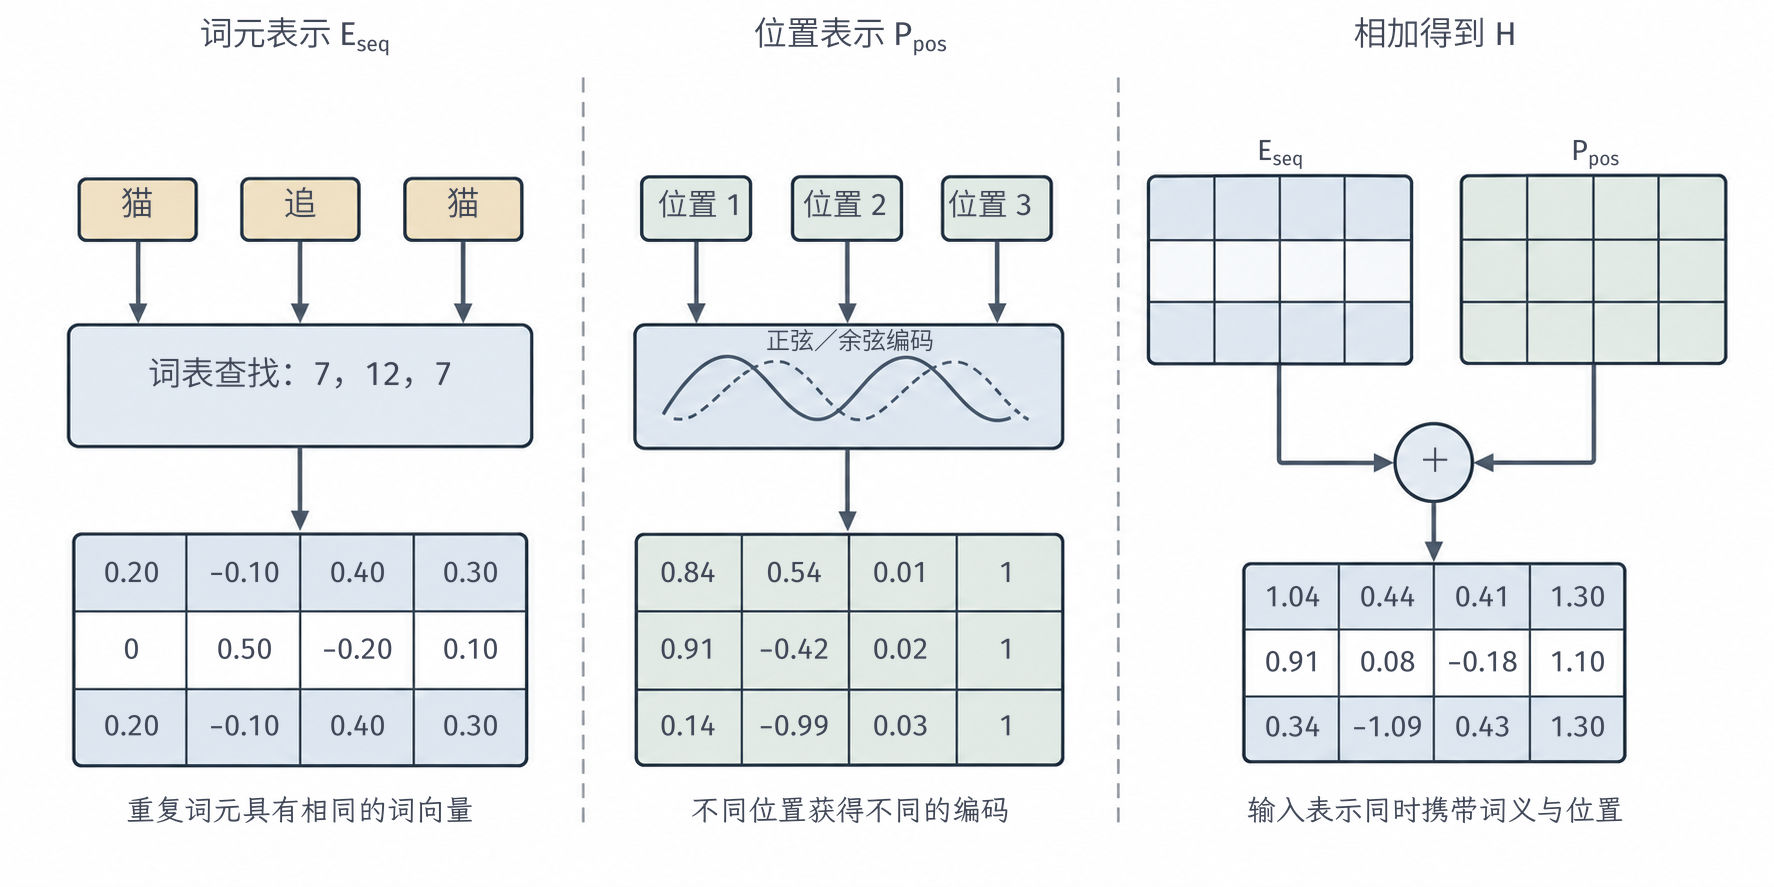
\includegraphics[width=150.199mm]{figures/05-neural-network-models/00-shared/generated/transformer-position-example/figure.png}
  \caption{序列“猫／追／猫”的输入构造。左图用词元编号查嵌入表，中图把位置序号代入正弦、余弦函数，右图将两组$3\times4$表示逐元素相加。三个矩阵的行均按输入位置排列，每格是一个特征值。两个“猫”共享内容向量，位置向量及最终表示却不同。词元编号和嵌入为教学设定；位置向量按弧度计算，数值保留两位小数，位置矩阵的最后一列显示相同是舍入所致。}
  \label{fig:transformer-position-example}
\end{figure*}

位置差异需要以能够留在后续表示中的方式编码。仅把编号$i$填在各坐标上，会遇到均值消除问题。例如，后文第\ref{sec:transformer-residual-normalization}节介绍的层归一化会减去一行的均值；若输入只加$i\bm1$并立即按行归一化，这个位置常数就会被消去。不同频率或可学习坐标提供了更丰富的位置差异。内容与位置进入同一表示后，训练才能据任务目标调整它们的组合与读取。

不等长序列可以填充到共同形状，真实位置由有效集合或长度记录。注意力排除填充键，池化只汇总真实位置，损失只统计有效监督位置。若将多段独立文本装入同一矩阵，也需限制跨段读取，并明确位置编号的重置方式；矩阵中相邻不等于任务中连续。

\subsection{注意力层}
\label{sec:transformer-attention}

第\ref{sec:transformer-attention-history}节已经介绍了注意力怎样根据当前需求读取信息。可以先把一次读取类比为查字典：手中待查的词是\term{查询}（query, Q），字典里用于匹配条目的词头是\term{键}（key, K），找到条目后读取的释义是\term{值}（value, V）。查询提出当前需求，键提供匹配特征，值提供被取出的内容；注意力中的键因此是表示向量，数组下标只负责存放它。

注意力把这种查询推广为连续的软匹配。输入经可学习投影得到查询、键和值，查询与键的连续得分再变成权重；多个值依权重共同形成输出。投影参数随训练调整，匹配方式也随之改变。这里把输入固定为“猫／追／狗”：更新“追”的表示时，网络需要结合谁在追、追的是谁；更新“猫”时，所需的上下文组合又可能不同。同一个位置在读取别人和被别人读取时承担不同作用，查询与键用于评分，值用于输出，三者不需要具有相同含义。

设查询输入为$\bm H_{\mathrm q}\in\mathbb R^{n_q\times d}$，被读取输入为$\bm H_{\mathrm s}\in\mathbb R^{n_s\times d}$。暂省略偏置，单头投影为
\begin{equation}
  \begin{aligned}
    \bm Q&=\bm H_{\mathrm q}\bm W_{\mathrm q},\qquad
    \bm K=\bm H_{\mathrm s}\bm W_{\mathrm k},\\
    \bm V&=\bm H_{\mathrm s}\bm W_{\mathrm v}\text{，}
  \end{aligned}
  \label{eq:transformer-qkv}
\end{equation}
其中$\bm W_{\mathrm q},\bm W_{\mathrm k}\in\mathbb R^{d\times d_k}$，$\bm W_{\mathrm v}\in\mathbb R^{d\times d_v}$；$\bm Q$、$\bm K$分别有$n_q$、$n_s$行和$d_k$列，$\bm V\in\mathbb R^{n_s\times d_v}$。若两侧宽度不同，只需分别调整投影的输入维度。评分公式规定权重怎样计算，信息来源规定键值来自哪里，可见范围规定哪些位置参与，头数则规定并行读取的组数。这些设置可以在一次注意力计算中共同使用。

\subsubsection{缩放点积注意力}

\term{缩放点积注意力}（scaled dot-product attention）把所有查询与键的点积转为权重，再聚合值。令固定掩码$\bm M$的形状为$n_q\times n_s$，各元素取$0$或$-\infty$：允许读取时$\bm M_{i,j}=0$，禁止读取时为$-\infty$。这里允许掩码取扩展实值，$-\infty$表示该项不参与归一化。一次前向计算为
\begin{equation}
  \begin{aligned}
    \bm S&=\frac{\bm Q\bm K^{\top}}{\sqrt{d_k}}+\bm M,\\
    \bm A_{i,j}&=\frac{\exp(\bm S_{i,j})}
      {\sum_{t=1}^{n_s}\exp(\bm S_{i,t})},\\
    \bm Z&=\bm A\bm V\text{。}
  \end{aligned}
  \label{eq:transformer-attention}
\end{equation}
$\bm S\in(\mathbb R\cup\{-\infty\})^{n_q\times n_s}$，$\bm A\in\mathbb R^{n_q\times n_s}$，$\bm Z\in\mathbb R^{n_q\times d_v}$。禁止项按$\exp(-\infty)=0$处理，参与计算的每个查询须至少有一个有效键。第$i$行输出是$\bm z_i=\sum_j\bm A_{i,j}\bm v_j$，其中$\bm v_j=(\bm V_{j,:})^{\top}$。Softmax沿键的位置归一化，每一行只在允许读取的位置上分配总量为1的权重；各行独立归一化，并不要求每列之和也为1。

现在可以回看式\eqref{eq:transformer-permutation}。无掩码自注意力中，重排后的投影分别为$\bm P\bm Q$、$\bm P\bm K$和$\bm P\bm V$，所以得分是$\bm P\bm S\bm P^{\top}$。重排列只改变每行求和项的次序，不改变Softmax分母；重排行则将对应的权重行一起移动。因此新权重为$\bm P\bm A\bm P^{\top}$，输出满足
\[
  (\bm P\bm A\bm P^{\top})(\bm P\bm V)
     =\bm P\bm A\bm V=\bm P\bm Z\text{。}
\]
这就把前面的顺序缺口接到了具体读取公式：内容匹配随输入一起重排，计算本身没有给某个行号赋予先后含义。

分母$\sqrt{d_k}$针对点积宽度增加带来的波动。这是一个容易被略过、却对训练影响很大的细节：点积是$d_k$个乘积之和，参与求和的项越多，即使每项的取值尺度不变，总和也越容易出现较大的正值或负值。若直接用未缩放的点积作Softmax得分，维度稍大时得分差就会被整体放大，Softmax迅速接近“赢家通吃”的极端分布，梯度随之消失。除以$\sqrt{d_k}$的作用，正是把得分的典型波动校正回与维度无关的尺度。若改用$d_k$或固定常数，缩放后波动会有不同的宽度依赖。下面用一个初始化时的简化模型说明这种增长，并把它与Softmax的梯度联系起来\scite{vaswani2017}

\paragraph{从坐标方差得到缩放因子}
暂时省略位置下标，设$\bm q,\bm k\in\mathbb R^{d_k}$相互独立，各自坐标也相互独立，且每个坐标均值为0、方差为1。令$s=\bm q^{\top}\bm k$。对第$r$个乘积，有
\[
  \mathbb E[q_rk_r]=\mathbb E[q_r]\mathbb E[k_r]=0,\qquad
  \mathbb E[(q_rk_r)^2]=\mathbb E[q_r^2]\mathbb E[k_r^2]=1\text{。}
\]
不同坐标乘积之间的协方差为0，因此
\begin{equation}
  \begin{aligned}
    \mathbb E[s]&=\sum_{r=1}^{d_k}\mathbb E[q_rk_r]=0,\\
    \operatorname{Var}(s)
      &=\sum_{r=1}^{d_k}\operatorname{Var}(q_rk_r)
        +2\sum_{r<t}\operatorname{Cov}(q_rk_r,q_tk_t)\\
      &=d_k,\\
    \operatorname{Var}\!\left(\frac{s}{\sqrt{d_k}}\right)&=1\text{。}
  \end{aligned}
  \label{eq:transformer-attention-scale-variance}
\end{equation}
标准差是方差的平方根，所以点积的典型波动尺度为$\sqrt{d_k}$。用它作分母，可以消去由宽度引起的增长；若除以$d_k$，方差反而变成$1/d_k$，宽度越大，得分就越被压向0。

\paragraph{得分尺度怎样影响Softmax}
将一行得分记为$\bm s$、权重记为$\bm a=\operatorname{softmax}(\bm s)$，其导数为
\begin{equation}
  \frac{\partial a_j}{\partial s_t}
      =a_j(\delta_{j,t}-a_t)\text{，}
  \label{eq:transformer-softmax-scale-gradient}
\end{equation}
其中$\delta_{j,t}$在$j=t$时为1，否则为0。若某个得分远大于其余得分，对应权重接近1，其他权重接近0，这些导数都会很小。对于只有两个键的情况，令$\Delta=s_2-s_1$，则$a_2=1/(1+e^{-\Delta})$，且$\partial a_2/\partial\Delta=a_2(1-a_2)$；当$|\Delta|$很大时，导数趋于0。

例如，取$d_k=64$，若未缩放的两个得分为$(0,8)$，第二个权重约为$0.9997$，对得分差的导数约为$0.00034$；除以$\sqrt{64}=8$后，得分为$(0,1)$，权重约为$0.7311$，对缩放后得分差的导数约为$0.1966$。若比较反传到同一个原始点积差$r$的梯度，还要计入缩放的导数：
\[
  a_2=\frac{1}{1+\exp(-r/\sqrt{d_k})},\qquad
  \frac{\partial a_2}{\partial r}
    =\frac{a_2(1-a_2)}{\sqrt{d_k}}\text{。}
\]
在本例$r=8$时，该导数约为$0.1966/8=0.02458$，仍大于未缩放时的$0.00034$。这组教学数值说明缩放如何缓解由维度放大造成的过早饱和；具体输入的导数由得分差决定，注意力仍可形成尖锐权重。减去行最大值控制指数的数值范围，缩放改变得分差；两项操作承担不同作用。

独立、零均值和单位方差是上述初始化模型的条件。训练后的查询与键可能相关，坐标尺度也会改变；自注意力还让二者来自同一输入，因此实际得分需要按当前表示评价。$1/\sqrt{d_k}$控制的是宽度带来的系统性变化，并不保证任意训练阶段的得分方差恰好为1。

\begin{example}[同一查询在不同可见范围内的读取]
  \label{ex:transformer-attention-numerical}
  对“猫／追／狗”中第2个位置“追”发起的查询，设$d_k=1$、$q_2=1$，三个词元的键依次为$0,\log2,0$，值依次为$(1,0)^{\top}$、$(0,2)^{\top}$、$(1,1)^{\top}$。这些是投影后的教学数值，不表示真实模型必然这样关注句子。三个缩放得分为$(0,\log2,0)$，取指数后为$(1,2,1)$，归一化得到权重$(1/4,1/2,1/4)$。输出为
  \[
    \bm z_2=\tfrac14(1,0)^{\top}+\tfrac12(0,2)^{\top}
                    +\tfrac14(1,1)^{\top}
             =(1/2,5/4)^{\top}\text{。}
  \]
  这个向量是“追”的新表示，不是直接选出一个词。三份二维值的贡献都进入这一表示，各自比例由权重给出。若改成因果读取，当前位置尚不能看到“狗”，得分变成$(0,\log2,-\infty)$，权重相应变为$(1/3,2/3,0)$，输出为$(1/3,4/3)^{\top}$。因果掩码使Softmax在前两个位置上重新归一化，原来的四分之一、二分之一比例也随候选范围改变。
\end{example}

图~\ref{fig:transformer-attention}先画出输入经三组参数投影得到查询、键和值，再把“追”的读取拆成评分、归一化和加权求和。查询与键决定“读多少”，值决定“读到什么”。键参与评分，值进入加权输出，混合结果可以与所有输入值都不同。损失因此同时影响评分权重和值特征，后文分别推导两条梯度路径。

\begin{figure*}[htbp]
  \centering
  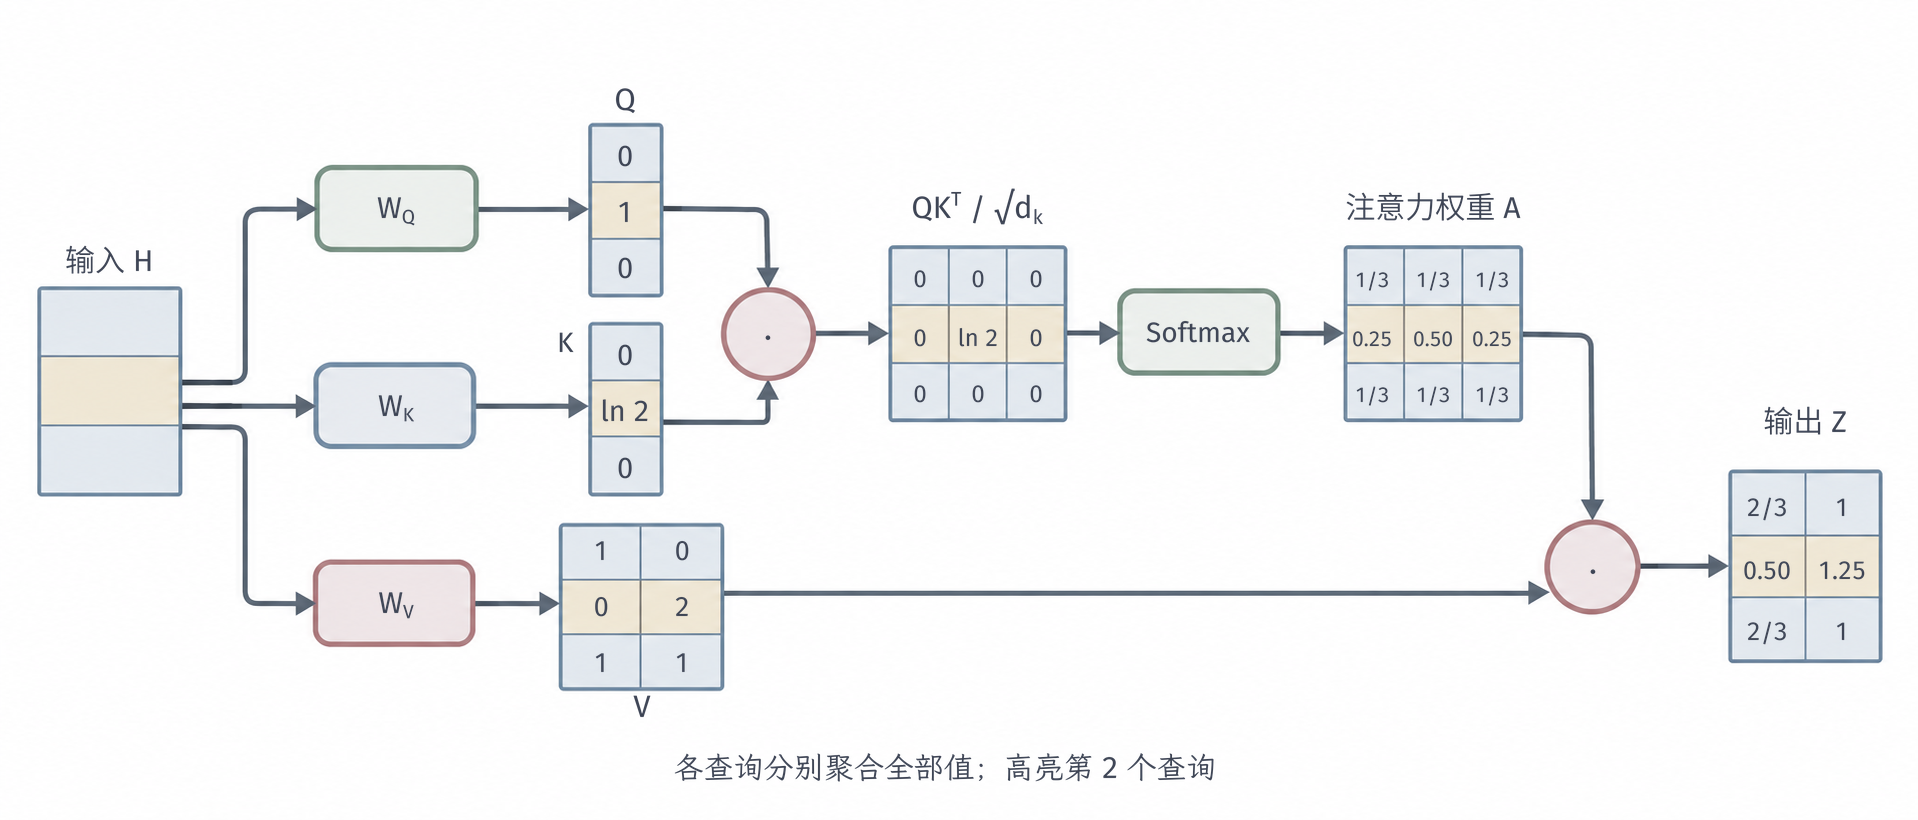
\includegraphics[width=162.391mm]{figures/05-neural-network-models/00-shared/generated/transformer-attention/figure.png}
  \caption{三个位置的缩放点积注意力，突出显示“追”这一查询。输入分别经三组投影产生查询$\bm Q$、键$\bm K$和值$\bm V$，三者各行依次对应猫、追、狗。突出显示的查询为$q_2=1$，与全部键匹配得到三个得分。Softmax按查询行产生权重矩阵，随后与值矩阵相乘得到各行输出；突出显示的一行权重为$(0.25,0.50,0.25)$，输出为$\bm z_2^{\top}=(0.50,1.25)$。浅色单元格示意矩阵数据，强调色标明同一查询的评分、权重与输出；$d_k=1$、$d_v=2$，数值均为教学设定。}
  \label{fig:transformer-attention}
\end{figure*}


\subsubsection{自注意力：同一序列内部读取}

上下文理解需要让一个输入位置结合其他输入位置。自注意力在式\eqref{eq:transformer-qkv}中取$\bm H_{\mathrm q}=\bm H_{\mathrm s}=\bm H$，查询、键和值都由同一组位置投影，得分矩阵为$n\times n$。

在看具体计算前，先回答一个自然的疑问：既然查询、键、值都来自同一序列，为什么还要用三组不同的投影，而不是让每个位置只带一个向量、自己跟自己点积？原因在于同一个位置在一次读取中要同时扮演三种角色。当它发起读取时，需要一个“我在找什么”的向量（查询）；当它被别人评估时，需要一个“我能提供什么线索”的向量（键）；被选中之后，真正传递出去的内容又是另一个向量（值）。一个位置发起查询时关心的特征，和它作为候选时值得被匹配的特征，以及它实际携带的信息，往往并不相同。三组独立可学习的投影，正是把这三种职责拆开，让训练分别调整“怎么找、怎么被找、给出什么”。因此三组投影各有参数；即使共享输入，通常也有不同的查询、键和值，只有特定参数设置才会得到$\bm Q=\bm K=\bm V$。为使三组线性投影可以逐项核对，图中取教学输入$\bm H=\bm I_3$，三组投影矩阵分别取为图示的$\bm Q$、$\bm K$、$\bm V$；独热输入让投影矩阵的每一行可直接对应图示数值，真实词元则通常使用前面定义的内容与位置表示。图~\ref{fig:transformer-self-attention}单独展开“追”的查询：三个位置提供值，按对应权重合成输出。中图权重表按查询位置排列，第2行就是$(0.25,0.50,0.25)$。若同一组键对应的另外两个查询取$q_1=\log_2 3$、$q_3=-1$，就分别得到第1行$(0.2,0.6,0.2)$和第3行$(0.4,0.2,0.4)$。查询不同，即使候选键值相同，读取也可以不同。整段输入可见时，各有效位置都在候选集合内，具体读取比例仍随查询与键改变。

\begin{figure*}[htbp]
  \centering
  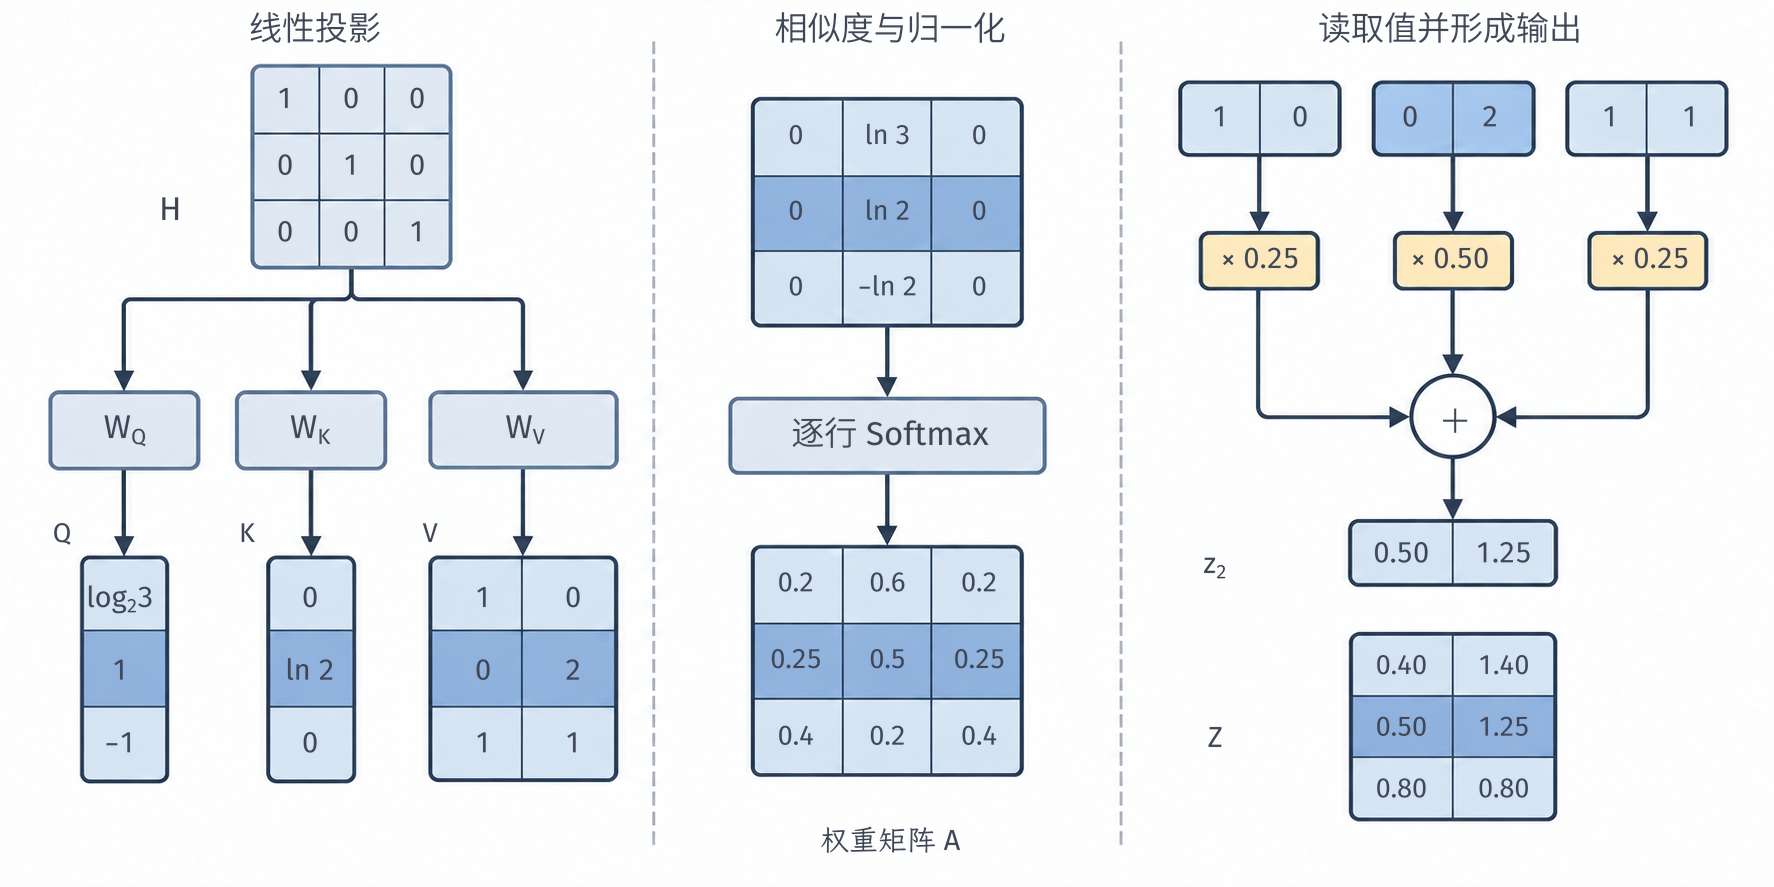
\includegraphics[width=150.199mm]{figures/05-neural-network-models/00-shared/generated/transformer-self-attention/figure.png}
  \caption{同一序列“猫／追／狗”上的自注意力。左图将教学输入$\bm H=\bm I_3$分别投影为查询、键和值；中图展示得分及逐行Softmax，行对应查询位置，列对应被读取位置。右图展开第2个查询，将三个二维值按$(0.25,0.50,0.25)$加权，得到$\bm z_2^{\top}=(0.50,1.25)$；下方矩阵汇总各查询分别计算的输出。$d_k=1$、$d_v=2$，所有数值为教学设定。}
  \label{fig:transformer-self-attention}
\end{figure*}

\FloatBarrier
\subsubsection{交叉注意力：从另一组表示读取}

目标序列需要读取源序列时，双方长度和职责通常不同。\term{交叉注意力}（cross-attention）让$\bm H_{\mathrm q}$提供查询，另一组$\bm H_{\mathrm s}$提供键和值，得分矩阵为$n_q\times n_s$。例如翻译目标当前位置用自己的状态提出查询，读取已编码的源句；每个查询产生一行输出，被读取侧提供键和值。以翻译“猫／追／狗”为例，图~\ref{fig:transformer-cross-attention}同时展开两个已知目标输入位置BOS和cat。BOS位置的输出用于预测cat，cat位置的输出用于预测chases；这两个目标状态产生两行查询，三个源编码状态产生三行键和值。源、目标长度不同，输出仍按目标查询排列，因此$\bm A$为$2\times3$，而$\bm Z$只有两行。

为了逐项算出一次交叉读取，取$d_k=1$，设目标投影后的查询为$\bm Q=(0,1)^{\top}$，源投影后的键为$\bm K=(0,\ln8,0)^{\top}$，值沿用前例的三个二维向量。BOS的三个得分都为0，Softmax给出$(1/3,1/3,1/3)$；cat的得分为$(0,\ln8,0)$，取指数得到$(1,8,1)$，归一化后为$(0.1,0.8,0.1)$。两行分别乘以同一个$\bm V$，得到$\bm z_1=(2/3,1)^{\top}$和$\bm z_2=(0.2,1.7)^{\top}$。后者对应cat发起的查询，供该目标位置后续预测使用。这一教学构造演示连续加权；真实翻译权重由训练形成，可能同时读取多个源位置。交叉注意力也可用于一种模态读取另一种模态；信息来源改变，不要求评分公式改变。

\begin{figure*}[htbp]
  \centering
  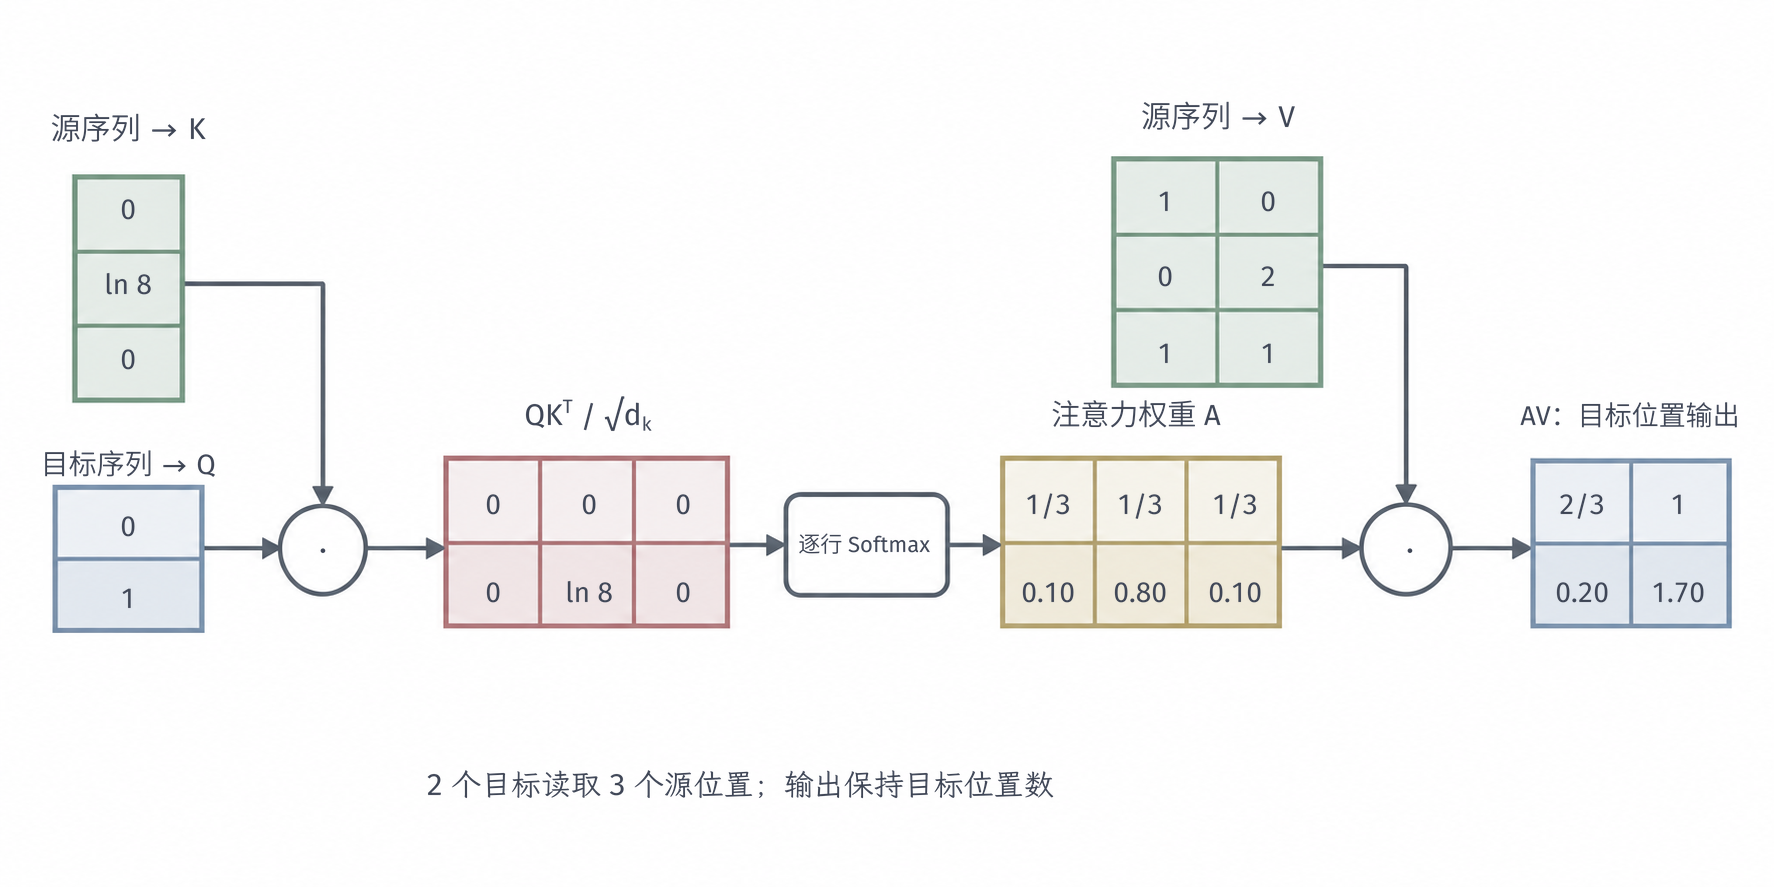
\includegraphics[width=150.199mm]{figures/05-neural-network-models/00-shared/generated/transformer-cross-attention/figure.png}
  \caption{两条不同序列的交叉注意力。目标输入BOS／cat的状态投影为两行查询，源输入猫／追／狗的编码状态分别投影为三行键和值。得分与权重矩阵的行对应目标查询、列对应源词元，因此形状均为$2\times3$；权重矩阵乘以$3\times2$的值矩阵后，输出为$2\times2$。较深的单元格突出cat这一目标位置从查询、评分、归一化到输出的对应关系。$d_k=1$，所有投影数值均为教学设定。}
  \label{fig:transformer-cross-attention}
\end{figure*}

交叉读取还说明了为什么输出长度跟随查询侧。假如只需要预测一个目标词，就只有一个目标查询，但它仍可读取全部源位置；源句变长会增加这一行的候选项，不会增加本步输出的行数。反过来，训练时同时提供多个目标查询，只是把多次读取排成多行，各行的权重仍分别归一化。源词与目标词因而不需要一一对应，一个目标词可以综合多个源位置，同一源位置也可以参与多个目标词的预测。

\subsubsection{因果注意力：只读取已知前缀}

同一序列也可能包含尚不能用于当前预测的未来内容。这个约束在逐词生成时是硬性的：预测第$i$个词时，第$i$个词本身以及它之后的内容还不存在，若网络在训练时“偷看”到了答案，学到的就不是据前缀预测，而是直接抄写。\term{因果注意力}（causal attention）通常指带因果掩码的自注意力，规定位置$i$只能读取$j\leq i$的键值，用结构保证这种泄漏不可能发生。图~\ref{fig:transformer-causal-attention}把“猫／追／狗”的可见范围直接排成矩阵。更新“追”时，“狗”所在格被屏蔽；“追”的输出经后续计算用于预测“狗”，因此输入位置和预测标签正好错开一步。它改变候选集合，投影与聚合公式仍为式\eqref{eq:transformer-attention}。训练把真实序列同时放入矩阵，各层的因果掩码共同保证前缀条件。前层若读取未来，后层接收到的表示已含未来内容，最后一层的掩码无法逆转这份混合。

\begin{figure*}[htbp]
  \centering
  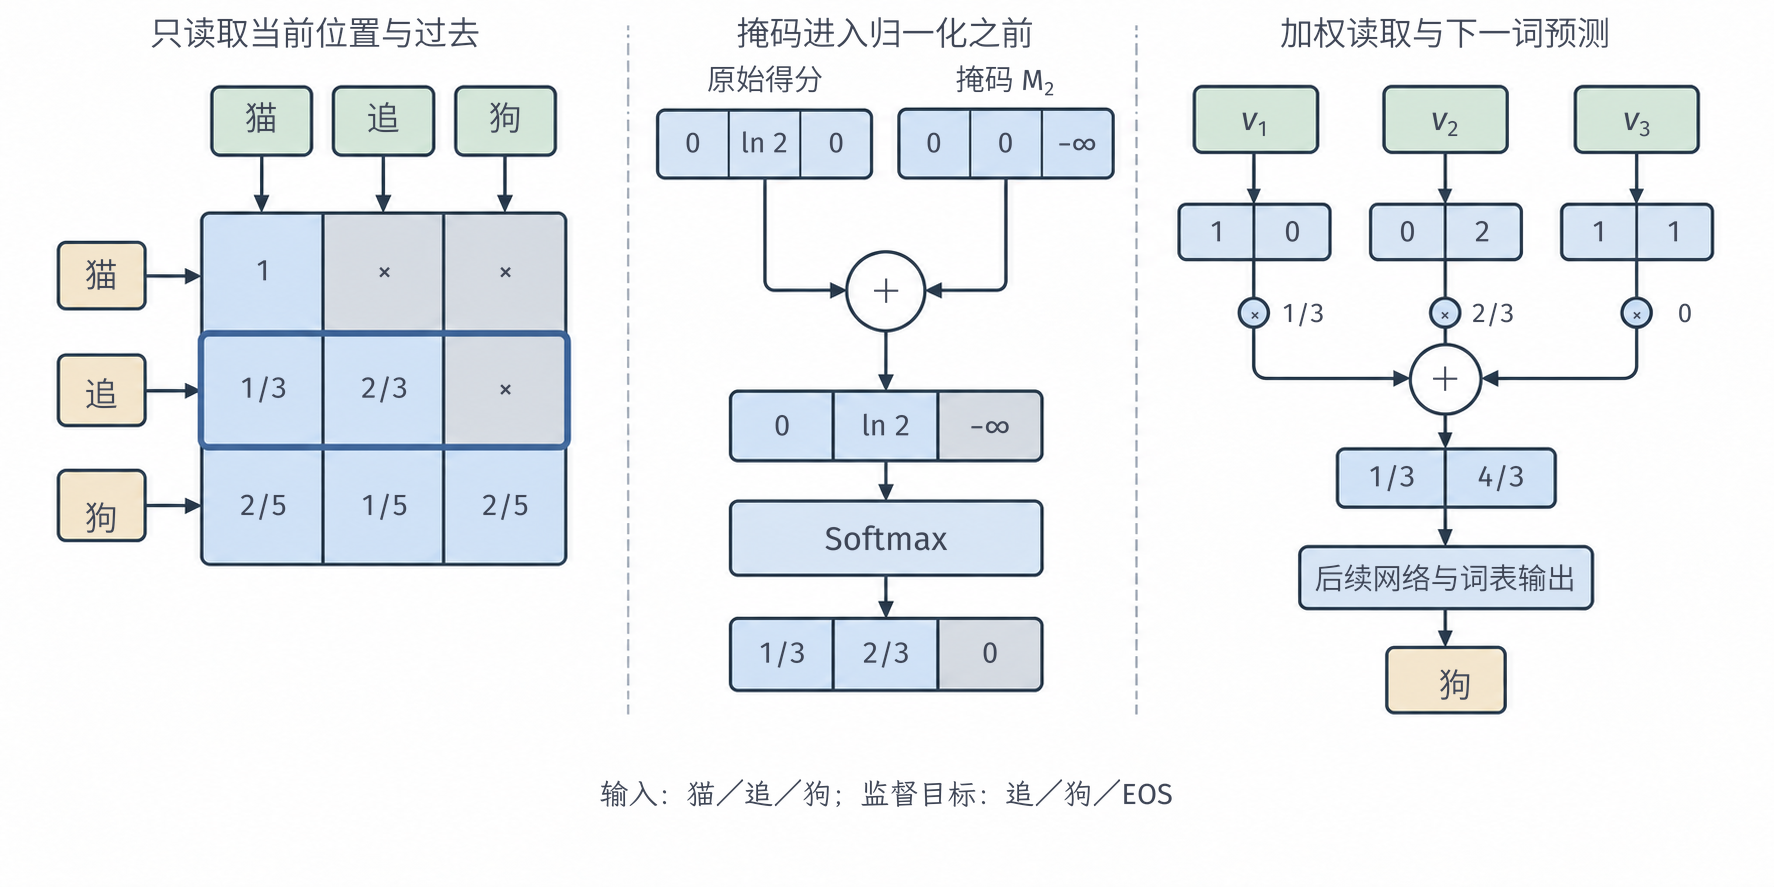
\includegraphics[width=150.199mm]{figures/05-neural-network-models/00-shared/generated/transformer-causal-attention/figure.png}
  \caption{“猫／追／狗”的因果自注意力。左图的行对应查询位置，列对应被读取的键；着色格给出可见位置的示例权重，浅灰叉号表示未来位置的权重为0。中图展开“追”这一行：原始得分先加因果掩码，再经Softmax得到$(1/3,2/3,0)$。右图加权读取值，得到$(1/3,4/3)^{\top}$，再经后续网络与词表头形成下一词元的预测分布；图中标出该位置的监督目标“狗”。预测“狗”时只读取当前已经给定的“猫／追”。底部展示错开一步的输入与监督目标，EOS为结束符；数值为教学设定。}
  \label{fig:transformer-causal-attention}
\end{figure*}
\term{填充掩码}（padding mask）阻止有效查询读取填充键；因果掩码排除未来位置。两者可以合并，前者排除不存在的输入，后者排除预测时尚不可知的信息。Softmax要求参与计算的查询至少有一个有效键；全行$-\infty$的指数归一化没有定义。填充查询可以跳过，也可以按有效规则得到随后弃用的输出，以便后续运算保持数值定义。因果掩码允许读取当前输入，这与预测下一个目标的移位配合，才构成没有目标泄漏的生成模型。

\subsubsection{多头注意力：并行形成不同的读取}

单组权重把各值压缩为一个混合。这会带来一个潜在问题：当一个位置需要同时关注几类性质很不同的信息时，单组权重被迫做一次性折中，混合后的向量里各类线索彼此纠缠，后续层很难再干净地分开。多头注意力的思路，就是并行地做几次关注点不同的读取，把各自结果原样保留下来再交由后续组合。\term{多头注意力}（multi-head attention, MHA）使用$h$组投影分别读取，再把结果拼接：
\begin{equation}
  \begin{aligned}
    \bm Z_a&=\operatorname{Attention}(\bm Q_a,\bm K_a,\bm V_a),\\
    \bm C&=\operatorname{Concat}(\bm Z_1,\ldots,\bm Z_h),\\
    \operatorname{MHA}(\bm H_{\mathrm q},\bm H_{\mathrm s})
      &=\bm C\bm W_{\mathrm o}\text{。}
  \end{aligned}
  \label{eq:transformer-multihead}
\end{equation}
头编号$a\in\{1,\ldots,h\}$，$\bm C\in\mathbb R^{n_q\times hd_v}$，$\bm W_{\mathrm o}\in\mathbb R^{hd_v\times d}$。常取$d_k=d_v=d/h$，使总投影宽度固定。各头分别学习权重和值特征，输出投影再组合这些结果。某头形成什么信息选择，由训练和输入决定；头之间是否互补可以据实际响应检验。固定$d$时增加头数同时减小每头宽度，读取组数与每组特征容量之间形成取舍。

图~\ref{fig:transformer-multihead}展开同一序列上的两个注意力头。三个位置的表示只输入一次，再交给每个头各自的查询、键和值投影；不同的投影使各头能够形成不同的读取权重和值特征。每个头都输出三行向量，拼接时对齐相同位置，只扩展特征维。例如，“追”在两个头中的输出拼为$[\bm z_{2,1}^{\top},\bm z_{2,2}^{\top}]$，这一拼接只扩展当前行的特征维，序列位置数保持原样。输出投影$\bm W_{\mathrm o}$再混合这些特征。多头既可用于自注意力，也可用于交叉注意力；每头还可以施加因果或其他掩码。常见的生成模型因此可以同时采用因果约束、多头投影和自注意力。

\begin{figure*}[htbp]
  \centering
  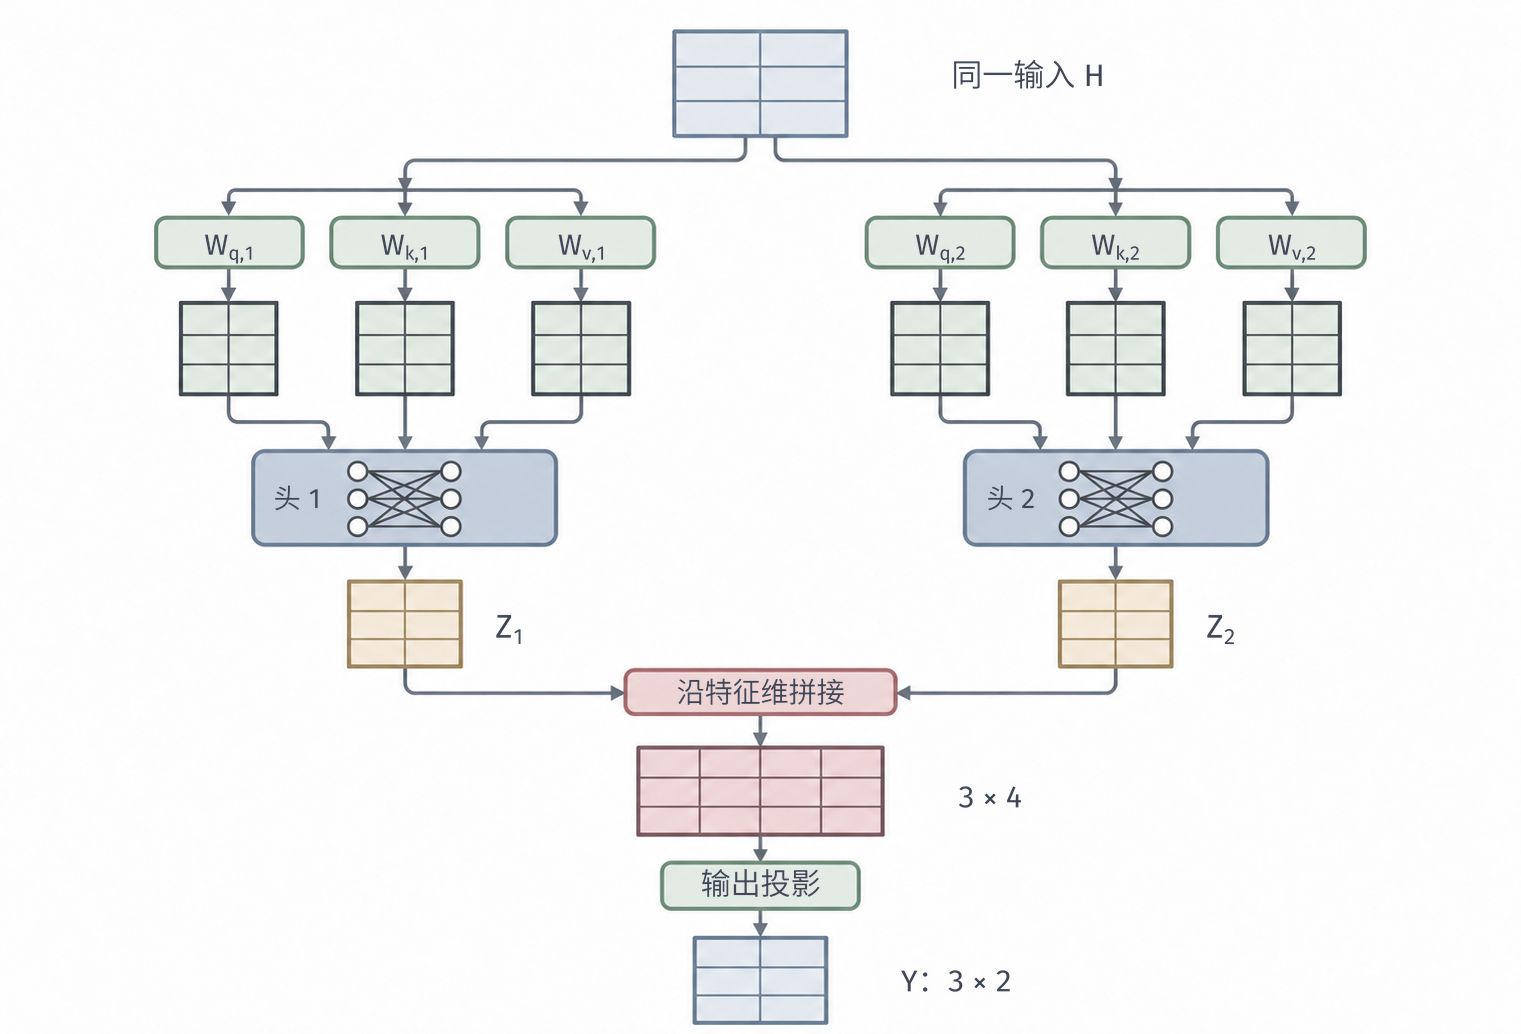
\includegraphics[width=128.778mm]{figures/05-neural-network-models/00-shared/generated/transformer-multihead/figure.png}
  \caption{同一输入序列上的两个注意力头。每个头分别学习$\bm W_{\mathrm q,a}$、$\bm W_{\mathrm k,a}$和$\bm W_{\mathrm v,a}$，独立完成评分、归一化和加权聚合，得到$\bm Z_a$。标有“沿特征维拼接”的框合并两路结果，两路输出的序列位置一一对齐，合并只增加特征宽度。拼接矩阵$\bm C$再经$\bm W_{\mathrm o}$投影，得到多头输出$\bm Y$。各头独立形成权重，输出投影组合它们的特征，具体信息分工由训练产生。}
  \label{fig:transformer-multihead}
\end{figure*}

可以把多头理解为先保留几份不同的读取结果，再决定怎样组合。假设两个头分别把“追”所需的主语线索和宾语线索读入不同特征，拼接保留了两组坐标，后续投影和FFN便可以对它们作不同处理。若先把两组结果平均为一个向量，这些差别可能在组合前就已丢失。这个例子说明多头结构提供的可能性；模型并没有预先为某个头规定“找主语”的职责，实际分工也可能重叠。

\subsection{前馈层}
\label{sec:transformer-feedforward}

注意力改变每个位置能读取什么，但读取结果还需转换为有用特征。这里要特别注意注意力本身做了什么、又没做什么：它本质上是对其他位置的向量做加权平均，只是把信息“搬运”并混合到当前位置，混合操作是线性的；若一个块里只有注意力，多层叠加所能表达的关系会受到很大限制。\term{逐位置前馈网络}（position-wise feed-forward network, FFN）补上的正是非线性加工这一环：它对每行单独使用同一组参数，先把特征投影到更宽的中间维度，在那里施加逐元素非线性、让不同特征相互组合，再投影回原来的隐藏宽度：
\begin{equation}
  \operatorname{FFN}(\bm H)
  =\phi(\bm H\bm W_1+\bm 1\bm b_1^{\top})\bm W_2
      +\bm 1\bm b_2^{\top}\text{。}
  \label{eq:transformer-ffn}
\end{equation}
其中$\bm W_1\in\mathbb R^{d\times d_f}$、$\bm W_2\in\mathbb R^{d_f\times d}$，$\bm b_1\in\mathbb R^{d_f}$、$\bm b_2\in\mathbb R^d$；$\bm 1$为$n$维全1向量，$\phi$逐元素作用。原始结构取$d_f=4d$并使用ReLU，其他结构可以采用第\ref{sec:ffn-activations}节介绍的激活函数和不同中间宽度。

每行使用同一FFN，输入内容和上下文不同，输出也随之不同。FFN在这一层不额外交换位置，它把已有上下文中的特征组合成新表示；下一次注意力再依据这些表示进行读取。若去掉非线性，两次仿射映射可以合成一次，扩张宽度本身就失去了增加非线性组合的作用。

这一层的参数量约为$2dd_f$，整段算术量为$O(ndd_f)$。长序列可能由位置对计算主导；短序列且$d_f$很大时，前馈计算和参数占比又会上升。完整成本需要同时计入注意力投影、聚合和前馈变换。

\subsection{残差连接与归一化}
\label{sec:transformer-residual-normalization}

层层变换时，可以让旧表示继续传递，同时学习需要增加的特征。这里遇到的是深层网络的普遍困难：若每个子层都必须把输入整体重写成输出，那么堆得越深，网络越难训练——梯度在层层连乘中容易放大或消失，而且多出的层至少不应把本来已经有用的表示改坏。\term{残差连接}（residual connection）把子层输出加到输入上，要求两者形状一致；这样每个子层只需学习在原表示之上“加一点什么”的增量，输入则保留一条畅通的直接传递路径，即使某层暂时学不到有用的东西，也可以把增量趋近于零、近似恒等地放行。注意力输出投影和FFN的维度恢复，也使这种相加可以在统一的$d$维空间进行。

不同位置的表示尺度还会影响点积和后续激活。随着层数叠加，表示向量的整体幅度可能逐渐变大或变小：注意力得分是点积，对幅度尤其敏感——若某些位置的向量范数很大，它们的点积会系统性地占优，Softmax便由幅度而非内容匹配主导，训练也容易失稳。\term{层归一化}（layer normalization, LayerNorm）在每个位置内部沿特征坐标计算均值和方差，不依赖其他样本或其他位置的统计量。之所以选择“沿一个位置自己的特征”统计，而不是像批归一化那样跨样本统计，是因为序列长度和批量大小经常变化、填充位置也不应参与，逐行归一化在训练和推理时都只依赖当前这一个位置，规则完全一致。对$\bm x\in\mathbb R^d$，令
\begin{equation}
  \begin{aligned}
    \mu(\bm x)&=\frac1d\sum_{k=1}^d x_k,\qquad
    s^2(\bm x)=\frac1d\sum_{k=1}^d(x_k-\mu(\bm x))^2,\\
    \operatorname{LN}(\bm x)
      &=\bm\gamma\odot
        \frac{\bm x-\mu(\bm x)\bm 1}{\sqrt{s^2(\bm x)+\varepsilon}}
        +\bm\beta\text{。}
  \end{aligned}
  \label{eq:transformer-layernorm}
\end{equation}
$\bm\gamma,\bm\beta\in\mathbb R^d$为可学习缩放和平移，$\varepsilon>0$避免分母为零，$\odot$表示逐元素乘法。应用于矩阵时按行计算，各位置共享$\bm\gamma,\bm\beta$。均值与方差只来自当前行，位置间模块再按任务掩码读取其他行\scite{ba2016layernorm}

原始Transformer把归一化放在残差相加之后，称为\term{后置层归一化}（post-layer normalization, Post-LN）。一个编码器块为
\begin{equation}
  \begin{aligned}
    \bm U^{(l)}&=\operatorname{LN}_{l,1}\!\left(
       \bm H^{(l-1)}+\operatorname{MHA}_l(\bm H^{(l-1)},\bm H^{(l-1)})\right),\\
    \bm H^{(l)}&=\operatorname{LN}_{l,2}\!\left(
       \bm U^{(l)}+\operatorname{FFN}_l(\bm U^{(l)})\right)\text{。}
  \end{aligned}
  \label{eq:transformer-postln-block}
\end{equation}
实际训练还可在子层输出加入Dropout，预测时关闭；这里省略它以突出确定性结构。\term{前置层归一化}（pre-layer normalization, Pre-LN）先归一化子层输入，再将子层输出加入原表示：
\begin{equation}
  \begin{aligned}
    \bm U^{(l)}&=\bm H^{(l-1)}+
      \operatorname{MHA}_l(\widetilde{\bm H}^{(l-1)},\widetilde{\bm H}^{(l-1)}),\\
    \widetilde{\bm H}^{(l-1)}&=\operatorname{LN}_{l,1}(\bm H^{(l-1)}),\\
    \bm H^{(l)}&=\bm U^{(l)}+
      \operatorname{FFN}_l(\operatorname{LN}_{l,2}(\bm U^{(l)}))\text{。}
  \end{aligned}
  \label{eq:transformer-preln-block}
\end{equation}
Pre-LN通常在整个堆叠末尾再归一化，之后交给输出层。图~\ref{fig:transformer-block}并列展开两种次序：Post-LN在残差相加后归一化，Pre-LN的跳跃路径则绕过归一化和子层；两者的学习性质将在第\ref{sec:transformer-normalization-extensions}节比较。同层各位置复用参数，后续层通常有自己的一组参数；额外的层间共享需要在模型中指定。

\begin{figure*}[htbp]
  \centering
  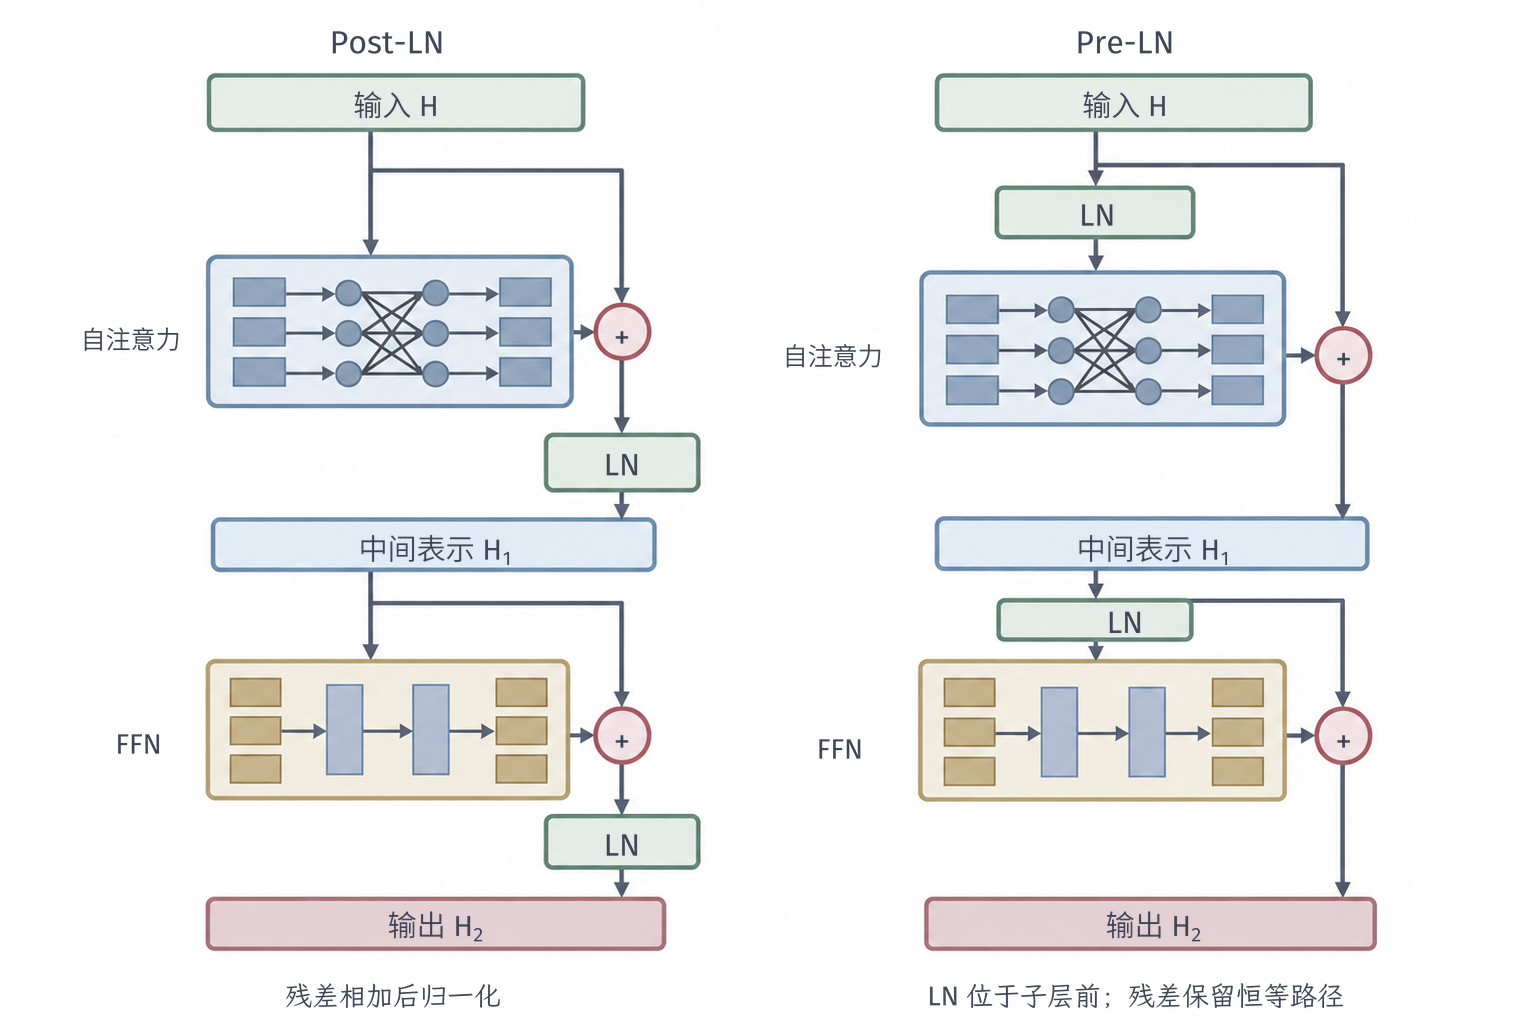
\includegraphics[width=128.778mm]{figures/05-neural-network-models/00-shared/generated/transformer-block/figure.png}
  \caption{Post-LN与Pre-LN编码器块的计算次序。输入与输出保持同一序列和特征形状。自注意力在行间交换信息，FFN分别变换各行；圆形$+$表示逐元素残差相加。图中箭头表示前向依赖；从残差路径可见，Post-LN的层间直达路径仍经过LN，Pre-LN则保留绕过归一化和子层的恒等支路。省略Dropout与Pre-LN堆叠末尾的归一化。}
  \label{fig:transformer-block}
\end{figure*}

\subsection{输出和网络架构}
\label{sec:transformer-architectures}

相同网络块可以用于不同预测过程，架构选择取决于输出对应哪些位置，以及这些位置在预测时能读取什么。在逐个认识模型之前，先抓住一个统一的判断方法：不要先记模型名字，而是先问两个问题——预测一个输出时，它被允许看到哪些位置（读取范围），以及损失落在哪一行表示上（监督位置）。整段分类只有一个答案，需要把$n$行汇成一个向量；词性标注每个词都有一个标签，损失落在每一行；翻译和续写下一个词尚未出现，必须因果读取。这三个问题一旦确定，编码器、解码器等“大块”如何摆放就基本确定了。\term{编码器}（encoder）通常让有效输入位置双向读取，形成整段上下文表示；\term{解码器}（decoder）在生成场景中使用因果自注意力，根据已知前缀预测后续输出。这里的“解码器”既可指原始编码器—解码器中的目标网络，也可指单独使用的因果网络，原始目标网络还读取源表示，单独因果网络则可以只读自身前缀。

\subsubsection{序列到分类或回归}

整段评论分类需要把$n$行表示转为一个向量。若最终输出表示为$\bm H$，有效位置集合为$V$，可以取$\bm r=|V|^{-1}\sum_{i\in V}\bm h_i$，再经分类头计算$\bm p=\operatorname{softmax}(\bm W_{\mathrm c}\bm r+\bm b_{\mathrm c})$。若有$c$类，$\bm W_{\mathrm c}\in\mathbb R^{c\times d}$，目标为$-\log p_y$。回归则用线性或受约束输出头形成数值，并选择与误差含义相符的损失。

另一种方式是在输入中加入专用读出词元，例如CLS，使用其末层表示$\bm r$。专用位置通过注意力读取整段，其输入参数、网络变换和任务头共同学习汇总方式。平均池化显式对位置等权，专用读出位置允许网络学习汇总，两者都要保证只读取任务允许的上下文。

\subsubsection{同步序列到序列}

词性或实体标签与输入位置对齐，可以对每行使用共享分类头，得到$\bm p_i$，在有效监督位置上计算平均交叉熵。离线标注可以读取完整输入；在线预测则需要因果掩码，或明确规定可等待多少后续位置。若预测下一时刻数值，目标还需移位。逐位置标签规定输出与输入的对应；离线、在线或有限延迟条件再规定每个输出可读的范围。

\subsubsection{异步序列到序列}

机器翻译的目标长度和源长度不同。\term{编码器—解码器}（encoder--decoder）先形成源表示$\bm H_{\mathrm s}$，目标网络在每层执行因果自注意力、交叉注意力和FFN。目标查询由该层已有的目标表示产生，键和值由最终源编码表示投影；源端填充掩码与目标端因果掩码分别约束两类读取。源表示供每个目标层重复读取，不必随着目标步重新编码；后文图~\ref{fig:transformer-architecture-original}用原始Transformer的翻译例子展示这条信息流。

给定源序列$x$，目标为$y_1,\ldots,y_m$，并将EOS计入目标，则条件分解为
\begin{equation}
  \begin{aligned}
    p_{\bm\theta}(y\mid x)
      &=\prod_{i=1}^{m}p_{\bm\theta}(y_i\mid x,y_{<i}),\\
    \ell(x,y)&=-\frac1m\sum_{i=1}^{m}
          \log p_{\bm\theta}(y_i\mid x,y_{<i})\text{。}
  \end{aligned}
  \label{eq:transformer-conditional-loss}
\end{equation}
$\bm\theta$包含输入、网络块和输出层参数。\term{教师强制}（teacher forcing）在训练时把真实目标前缀送入网络；目标输入是BOS、$y_1,\ldots,y_{m-1}$，目标标签是$y_1,\ldots,y_m$。全段输入已知，各位置可以并行计算，因果掩码保证第$i$个输出没有读到待预测的$y_i$。

条件生成也可用单个解码器：把源输入、分隔符和移位目标组织成同一序列，通常只在目标预测位置计算损失。使用全因果掩码时，源位置也只能读取其前缀；使用前缀掩码时，源位置可互相读取，目标位置可读取全部源前缀和此前目标。两种掩码都能服务于条件生成，源端表示的形成范围却不同。独立编码器—解码器另有源堆栈和交叉读取，三个计算组织应据各自依赖比较。

\subsubsection{序列续写与生成}

单独的因果解码器省略源交叉注意力，将已有文本本身作为条件。对词元$u_1,\ldots,u_n$，从BOS开始预测时，联合概率为$\prod_{i=1}^n p_{\bm\theta}(u_i\mid u_{<i})$。若最终表示$\bm h_i$对应第$i$个已输入词元，则下一词元概率为
\begin{equation}
  \bm p_{i+1}=\operatorname{softmax}
     (\bm W_{\mathrm{out}}\bm h_i+\bm b_{\mathrm{out}})\text{，}
  \label{eq:transformer-vocabulary-head}
\end{equation}
其中$\bm W_{\mathrm{out}}\in\mathbb R^{v\times d}$。可令$\bm W_{\mathrm{out}}=\bm E$进行输入输出嵌入共享，这使输入取出的内容向量和输出评分共用参数，限制了两接口可以独立调整的自由度。大词表投影还会产生$O(dv)$的单位置计算。

生成从已知前缀开始，计算下一词元分布，按指定策略选择一个词元，将其加入输入，再继续，遇到EOS或最大生成长度停止。贪心每步取当前条件下概率最大的词元，整段概率还随后续条件变化；采样则按指定分布产生词元。训练损失、预测时的选择策略和实际任务评价需分别说明。编码器适合已知完整上下文的理解，因果解码器适合按前缀生成，编码器—解码器使源与目标表示分开组织；输入何时可见与计算预算共同决定这些组织在实际任务中的适用范围。

\subsection{常见Transformer架构}
\label{sec:transformer-common-architectures}

前面按输出形式组织了网络，这里进一步比较几种实际模型。读这一节时容易陷入“背模型配置”的误区，更有价值的读法是把它们看成同一组构件在“读取范围＋预训练目标”两个维度上的不同选择：它们的注意力、FFN、残差几乎相同，真正不同的是允许每个位置读到什么，以及用什么任务在大规模无标注文本上预先训练。同样面对“猫追狗”，BERT可以补回被遮蔽的“追”，GPT可以根据“猫追”续写“狗”，编码器—解码器则可以把整句翻译成另一种语言。它们共享注意力与前馈计算，但读取范围、监督位置和生成过程不同。以下架构图沿用整序列的分层表示：长条作用于整段序列，虚线框表示重复堆叠，箭头表示前向信息依赖。BERT和RoBERTa另用公式展开一个Post-LN块，GPT则并列比较归一化次序。长条和块内公式分别说明词元读取与层间更新\scite{bishop2024deep} 各图都把中文例子按词划分，以便观察对应关系；这种教学划分不代表某个模型实际采用的子词分词器，图中的词元是监督目标或示例生成结果。

\subsubsection{原始Transformer：源与目标分开建模}

翻译时，源句通常已经完整给定，目标句却需要逐词产生。这两个条件不同，原始Transformer便用两组网络分别处理：编码器双向读取源句，解码器因果读取已有译文，再通过交叉注意力查询源表示。原论文基础模型的编码器和解码器各有6个块，隐藏宽度512，8个注意力头，FFN中间宽度2048，采用正弦位置编码、ReLU与Post-LN\scite{vaswani2017}

\begin{figure*}[t]
  \centering
  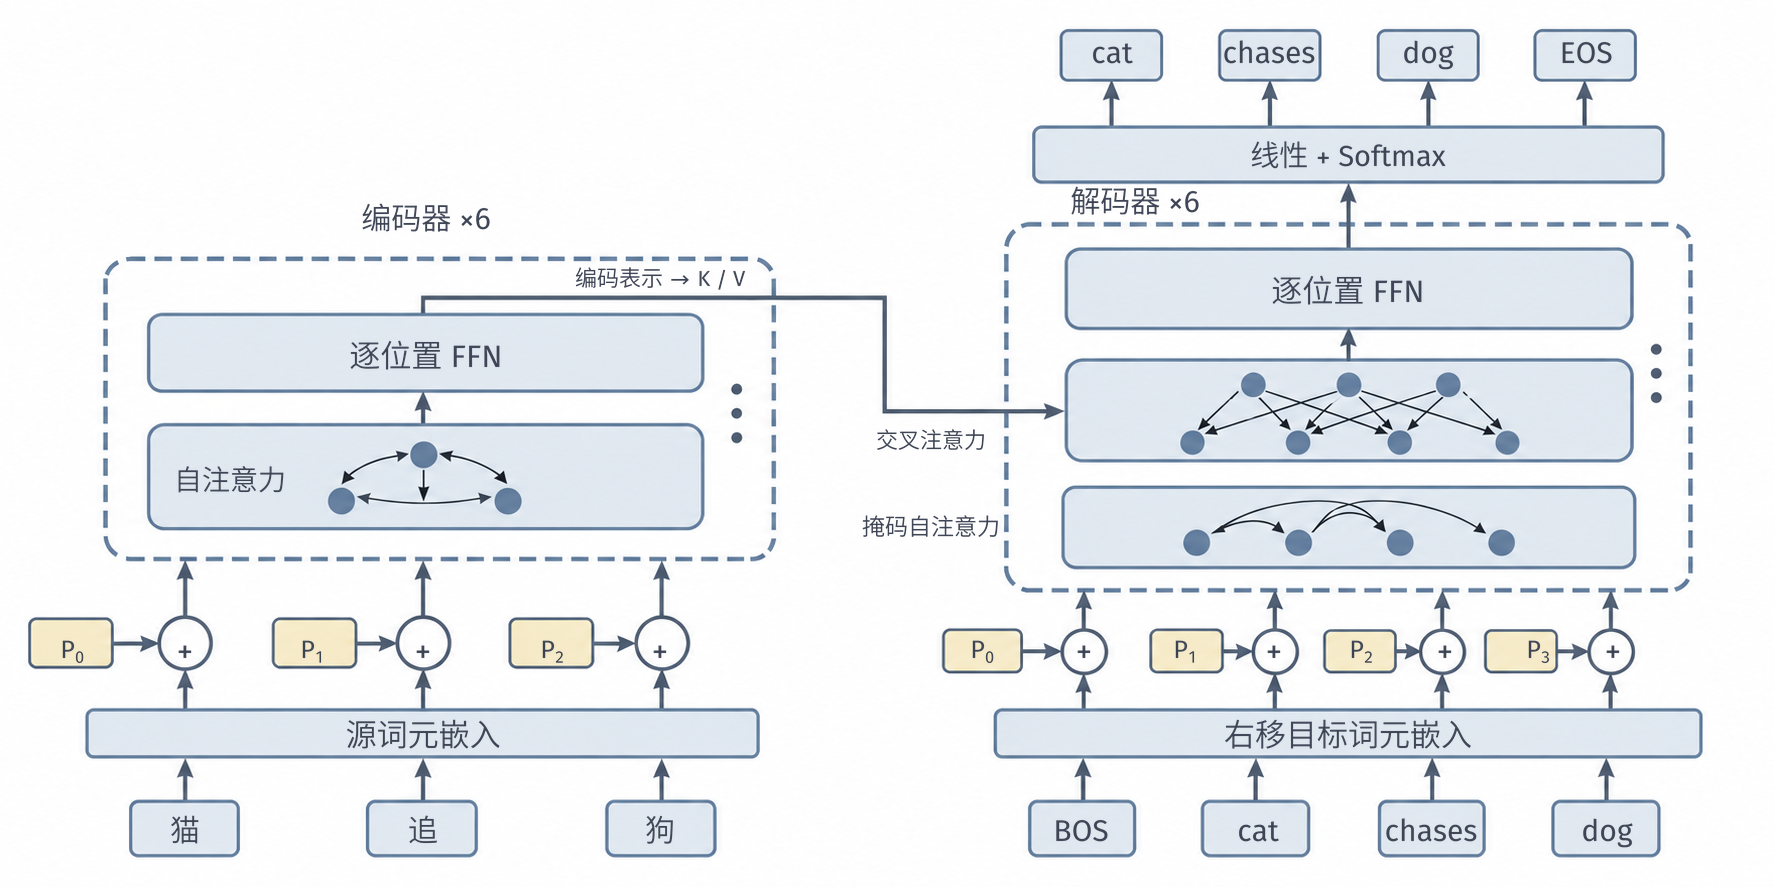
\includegraphics[width=150.199mm]{figures/05-neural-network-models/00-shared/generated/transformer-architecture-original/figure.png}
  \caption{原始Transformer基础模型的整网信息流。源编码器与目标解码器各堆叠6个块；每个长条作用于整段序列。解码器先因果读取目标前缀，再交叉读取最终源表示；各目标块据此生成K、V，Q来自各块的目标路径，不与同编号的中间编码层配对。目标输入右移，输出为对应的下一词元，最后预测EOS。省略残差、Post-LN、Dropout和嵌入缩放；结构依据Vaswani等（2017）。}
  \label{fig:transformer-architecture-original}
\end{figure*}

以“猫追狗”的翻译说明图~\ref{fig:transformer-architecture-original}的条件生成过程。训练时，解码器输入是右移的目标“BOS、cat、chases、dog”，对应监督目标是“cat、chases、dog、EOS”。预测dog的目标位置可以读取cat和chases，同时通过交叉注意力读取源句中的“狗”；“狗”的源词元属于已经给定的条件，目标词元dog则是这一位置需要预测的监督标签。推理时没有正确译文可供右移，解码器把自己已经生成的词元作为后续输入。

沿图中两条路径继续看，编码器输出的每一行已经结合源句上下文。源位置“狗”的表示不再只是词表中的“狗”，其中还可能包含它与“追”的关系。解码器也先用因果自注意力整理已经生成的目标前缀，再把这一层的目标表示用作查询。因此，交叉注意力读取的是“当前翻译状态需要什么源信息”，而不是直接拿一个孤立的英文词去查中文词表。查询随目标位置和网络层改变，源端最终表示则保持不变。

这里的“源表示保持不变”不表示所有解码器层共享同一套键和值。每个解码器层有自己的交叉注意力投影，将同一份最终源表示映射成该层的键和值；编码器的第1层也不会专门连接解码器的第1层。固定源句和模型参数后，各目标步复用每层各自的源投影。这样既能让不同层选择不同源特征，又能避免在每次生成时重新编码源句。

掩码可以用矩阵形状逐项核对。若源句有$n$个有效词元，移位后的目标输入有$m$个位置，则源自注意力的得分为$n\times n$，目标自注意力为$m\times m$，交叉注意力为$m\times n$。目标自注意力保留下三角，交叉注意力允许读取全部有效源位置；目标中尚未生成的词元不能通过第一条路径进入计算，完整源句则可以通过第二条路径参与预测。批量中的填充位置另行屏蔽，不计入这些有效长度。

参数学习最小化式\eqref{eq:transformer-conditional-loss}的条件负对数似然，编码器、解码器和词表头一起更新。教师强制允许并行计算所有目标位置，但生成时仍须逐步扩展前缀；训练用真实前缀而预测用自身输出，会使两种过程经历不同的输入分布。源投影和已有目标键值可以缓存，复用先前前向结果；新的目标词元仍在本步选择后进入下一步输入。

EOS也属于预测目标。以图中的译文为例，最后一个输入dog对应的标签为EOS，因此网络会学习在什么条件下结束，而不必让目标长度等于源长度。生成时若某一步选错了词，后续查询会沿错误前缀继续形成；训练时较小的单词预测损失，也不能保证逐步选择得到整段概率最大的译文。模型给出条件分布，解码方法再决定如何在这些分布上选择序列，两者需要分别评价。

源、目标长度还决定了两条路径各自的成本。固定隐藏宽度$d$，只统计一层的位置配对与聚合，源自注意力为$O(n^2d)$，目标自注意力为$O(m^2d)$，交叉注意力为$O(mnd)$。交叉项来自每个目标查询都要对$n$个源位置评分和读取；它不是源端平方项或目标端平方项的重复计算。实际整网还需乘上各自层数，并计入投影、FFN和词表输出；缓存减少重复工作，但不会让新查询免于读取所需源信息。

这种组织可以一次编码源句，并在多个解码步骤中复用源表示，源端也能充分结合左右语境，适合输入和输出边界明确的翻译、摘要等任务。代价是需要维护两组网络和交叉注意力；当任务只是从一个前缀继续写下去时，单一路径的因果模型通常更直接。成本比较还需固定源长、目标长、宽度和层数，两组堆栈及交叉注意力各占多少计算由这些配置决定。



\subsubsection{BERT：利用左右语境形成表示}

若目标是判断句意或标注每个词元，当前位置常常需要后文。\term{BERT}保留双向编码器，并使用\term{遮蔽语言模型}（masked language model, MLM）预训练：先扰动部分输入，再从上下文恢复原词元。例如输入“猫 [MASK] 狗”时，被遮蔽位置必须结合“猫”和“狗”预测“追”。原始BERT还通过CLS位置的表示预测两个句段是否相邻，即下一句预测（next sentence prediction, NSP）。BERT Base为12层、宽度768、12个头，Large版本为24层、宽度1024、16个头；输入叠加词元、可学习位置和句段嵌入，块内使用GELU与Post-LN\scite{devlin2019}

图~\ref{fig:transformer-architecture-bert}中，MLM只在选中的位置接受词元监督；用于分类时，则可以在CLS表示上接任务头。原始训练并非把每个选中位置都替换为[MASK]，还混合随机替换和保留原词，以减轻预训练输入与实际使用输入的差别。这里画出遮蔽分支，是为了突出双向上下文如何帮助恢复缺失内容。

\begin{figure*}[t]
  \centering
  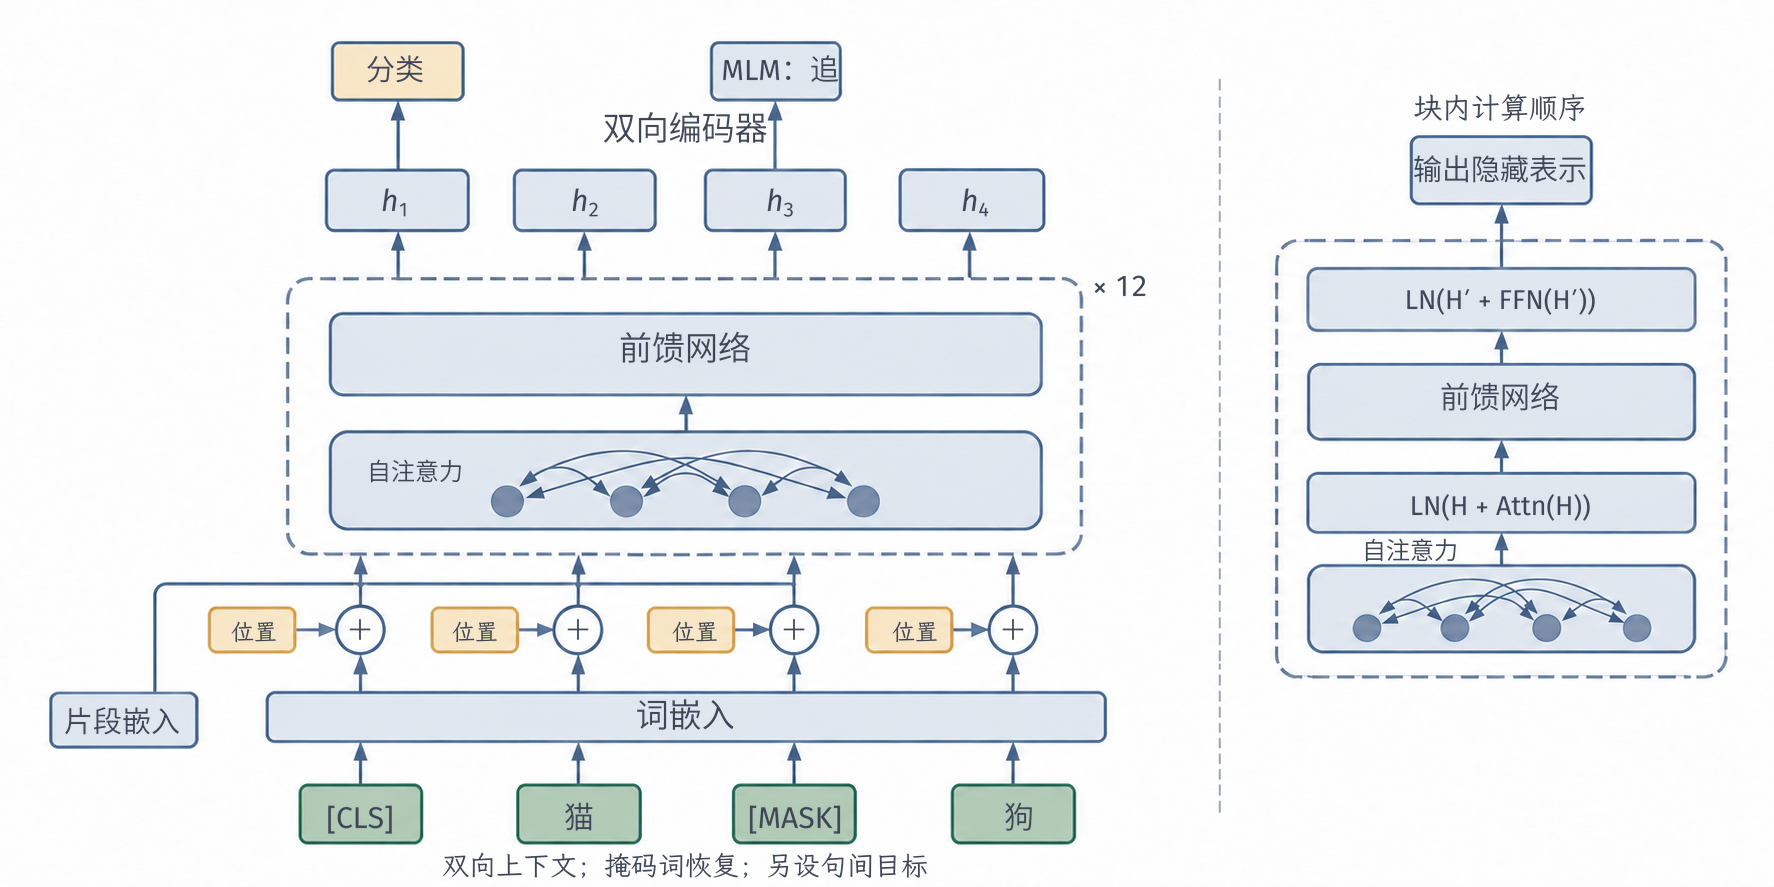
\includegraphics[width=150.199mm]{figures/05-neural-network-models/00-shared/generated/transformer-architecture-bert/figure.png}
  \caption{BERT Base的双向编码器与预测位置。词元、位置和句段嵌入相加，12个编码器块形成上下文表示；左侧画出一个短片段，省略分隔符。CLS用于序列分类，遮蔽位置由MLM头恢复“追”。主流程省略层内残差与归一化，右侧展开一个Post-LN块；$\operatorname{Attn}$、$\operatorname{FFN}$分别表示注意力与前馈变换，$\bm H'$表示注意力子层残差归一化后的输出。残差直接写入公式；省略Dropout与NSP头。结构依据Devlin等（2019）。}
  \label{fig:transformer-architecture-bert}
\end{figure*}

原始BERT随机选取约15\%的普通词元作为MLM监督位置，其中80\%改为[MASK]、10\%替换为随机词元、10\%保持原样。设选中集合为$M$、扰动输入为$\widetilde x$，词元损失为$-\sum_{i\in M}\log p_{\bm\theta}(x_i\mid\widetilde x)$；未选位置仍提供上下文，但不直接接受这项恢复监督。原始预训练还加上句段对的二分类损失。微调时换接任务头，使用任务标注继续更新编码器；冻结编码器只训练头则是另一种成本较低的使用方式。

微调所用的标签会改变信息汇总的方向。例如，判断“这部电影并不精彩”的情感时，CLS本身没有这句话的词义；它在多层自注意力中读取其他位置，分类损失再推动整个编码器保留与标签有关的线索。若改为给每个词元标注实体类型，就把监督接到各自的末层表示上。两种任务可以共享预训练参数，但读出位置与损失不同；预训练得到一个可供继续调整的表示起点，并未预先确定所有下游任务的分类规则。

双向读取使BERT适合在完整输入上做分类、抽取和序列标注；各位置表示可以在一次前向计算中并行形成。MLM按扰动输入恢复选中词元，定义了这种条件预测。自由续写还需要左到右或其他序列生成目标及对应解码过程。若当前位置读取了未经扰动的自身内容，恢复同一词元便有直接答案可用，因而目标和可见输入必须一起设计。



\subsubsection{RoBERTa：改进双向编码器的预训练}

BERT的效果还取决于预训练方式，而不仅是网络拓扑。\term{RoBERTa}保留BERT式双向编码器，主要改变训练配方：每次送入序列时重新抽取遮蔽位置，取消NSP，使用更大的批次、更多文本和更充分的训练，并改用字节级BPE词表。图~\ref{fig:transformer-architecture-roberta}沿用BERT式编码器，画出遮蔽“追”的一次训练输入；动态遮蔽表示不同次训练可以重新抽取遮蔽位置，让模型接触不同的上下文恢复问题\scite{liu2019roberta}

\begin{figure*}[t]
  \centering
  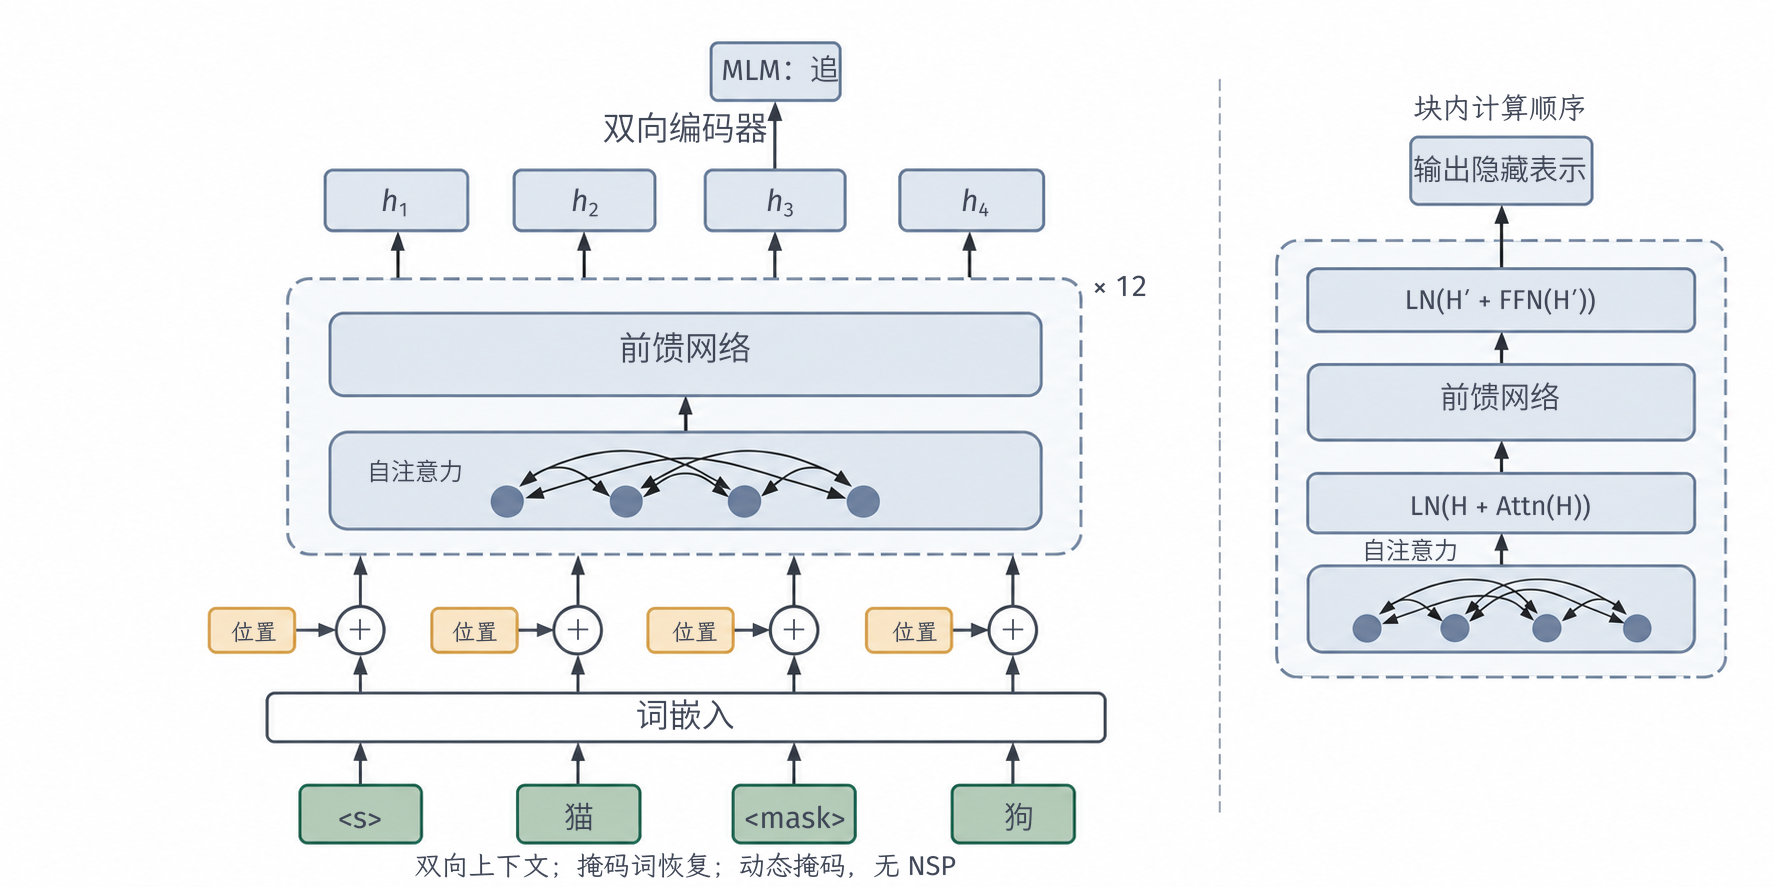
\includegraphics[width=150.199mm]{figures/05-neural-network-models/00-shared/generated/transformer-architecture-roberta/figure.png}
  \caption{RoBERTa Base的双向编码器与遮蔽恢复。词元与可学习位置嵌入相加，12个编码器块形成上下文表示，选中的遮蔽位置由MLM头恢复“追”。核心结构与BERT相同，预训练采用动态遮蔽且不使用NSP。主流程省略层内残差与归一化，右侧展开Post-LN计算次序；省略Dropout。训练差异依据Liu等（2019）。}
  \label{fig:transformer-architecture-roberta}
\end{figure*}

它仍在选中的位置计算MLM交叉熵，不同遮蔽样本通过同一网络分别前向；各样本内部双向读取，样本之间不交换词元。NSP是句段级训练目标，取消它改变了样本组织和损失；编码器内部的注意力模块保持原来的读取作用。下游分类或标注仍需把末层表示接到相应任务头，并明确哪些参数继续训练。

动态遮蔽改变的是什么，可以用同一句训练文本说明。一次输入“猫 [MASK] 狗”，要求恢复动作；另一次输入“[MASK] 追 狗”，要求恢复动作的发起者。底层词元序列相同，提供给网络的上下文和接受监督的位置却不同。于是，同一文本可以产生多种恢复问题。每次前向都需要按本次扰动重新计算双向表示，不能把上次遮蔽输入的中间结果直接当作这次的表示；图中展示的是其中一次扰动，而不是同时混合所有遮蔽结果。

RoBERTa以相同核心结构检验数据、目标与优化设置的作用。其预训练投入和方案同时变化，论文的整体收益应结合这些配置解释；单项改动的作用需要相应对照实验。两者在使用方式上仍然接近，都适合完整输入上的理解任务，也都需要额外设计才能作为自由续写模型。



\subsubsection{GPT：因果解码器及其版本演进}

续写时，模型只能依据已经出现的内容预测下一项。\term{GPT}家族由这一任务发展而来；早期公开的GPT-1、GPT-2和GPT-3都采用只有解码器的组织，每个块包含因果自注意力与FFN，没有独立源编码器，也没有连接源表示的交叉注意力。版本演进涉及块内计算、模型规模、训练目标和使用方式，以下分别说明它们改变的输入与参数。

\paragraph{GPT-1：建立预训练后微调的因果模型}

初代GPT于2018年采用12层、宽度768、12个头的结构，配合可学习绝对位置、GELU与Post-LN；先用下一词元预测进行语言模型预训练，再针对下游任务微调。为便于与后续版本区分，这里称其为GPT-1\scite{radford2018gpt}

图~\ref{fig:transformer-architecture-gpt}并列比较早期三个版本的计算次序。以词元序列说明监督：“猫”位置预测“追”，“追”位置预测“狗”。训练时三个位置可以一起计算，因为因果掩码已经阻止了未来信息进入各层表示；推理时则必须先选出“追”，才能把“猫追”作为下一步的前缀。把问题、示例或文档放在前缀中，后面接答案，就能沿同一条路径完成条件生成。

\begin{figure*}[htbp]
  \centering
  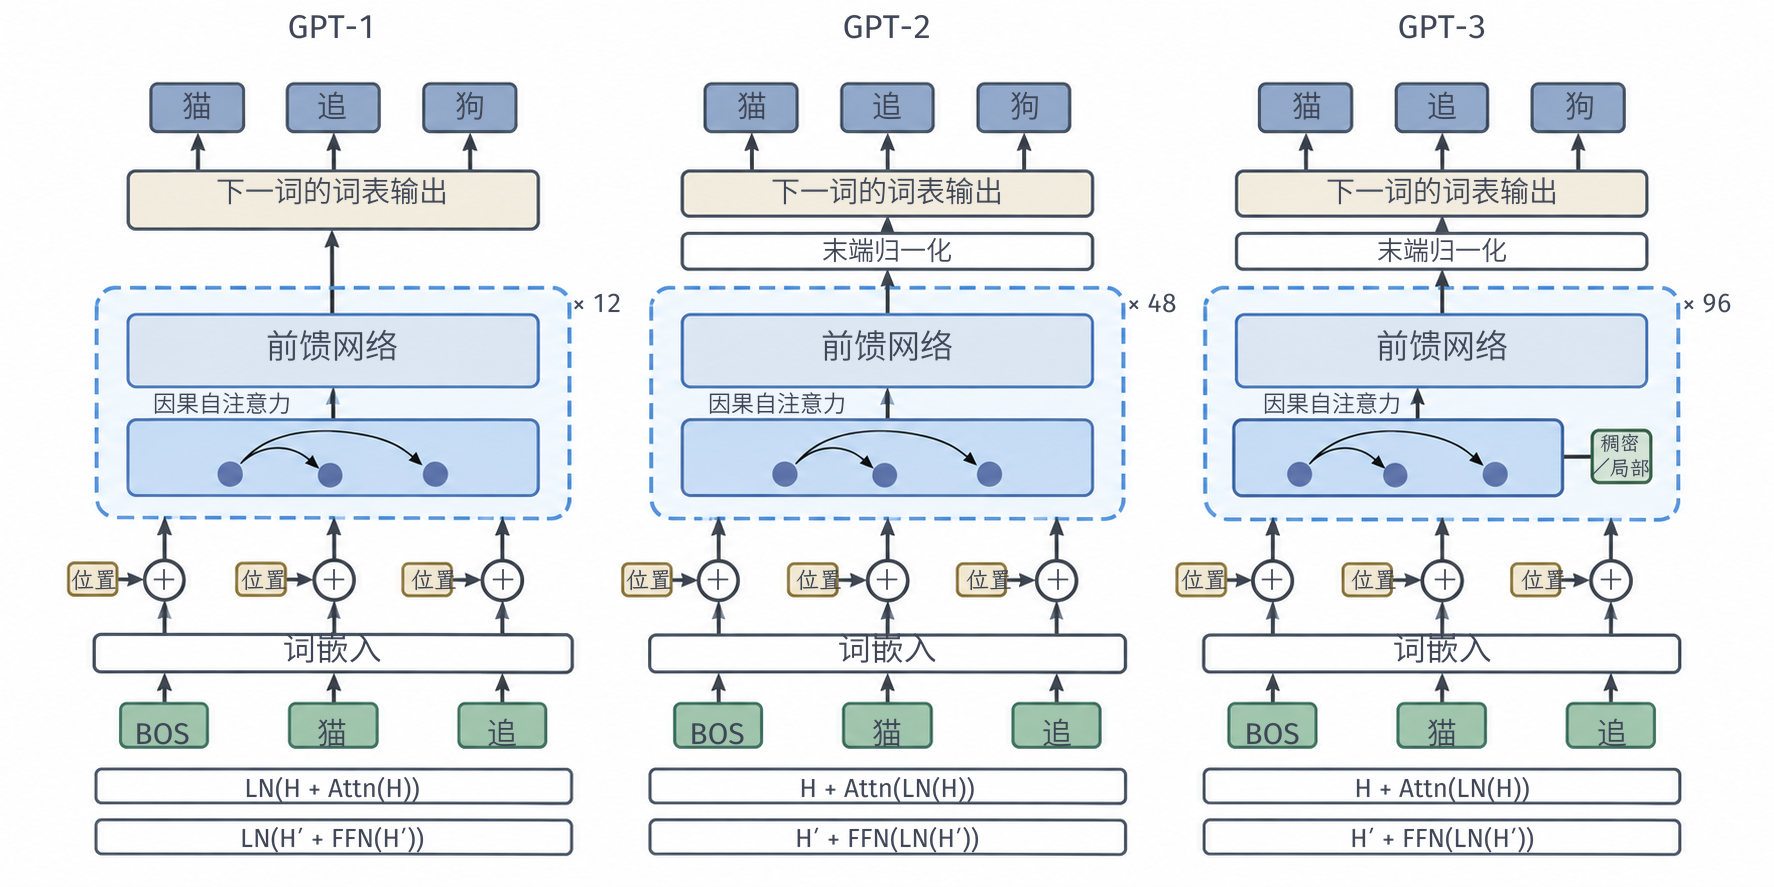
\includegraphics[width=150.199mm]{figures/05-neural-network-models/00-shared/generated/transformer-architecture-gpt/figure.png}
  \caption{GPT-1、GPT-2与GPT-3的公开块结构对比。各列下方的公式包括子层变换、残差和归一化；各版本中的$\operatorname{Attn}$均遵守因果约束。GPT-1采用Post-LN，GPT-2和GPT-3采用Pre-LN并增加堆叠末端归一化；GPT-3还交替使用稠密与局部带状注意力。层数指各原论文的最大公开配置，省略Dropout、内部投影和KV缓存；比较依据相应原论文。}
  \label{fig:transformer-architecture-gpt}
\end{figure*}

图中的竖直方向表示层数，水平方向表示词元位置。一次训练会让所有已知输入位置同时经过第1层，再同时经过第2层，依此向上；因果约束由每层的连接范围保证。生成时，前缀虽已知，尚未选出的下一词元却没有输入嵌入，因此不能提前计算它的各层表示。这就是“训练可以并行处理位置”和“生成仍逐词进行”能够同时成立的原因：两句话讨论的是不同阶段的已知输入。

同样以情感分类为例，GPT-1的预训练先学习文本接续，有监督微调再把句子末位置的表示接到分类头，并用类别标签更新模型。末位置可以因果读取整句，早期位置仍只能读取此前内容。原论文还在微调中保留辅助语言模型目标，让任务分类与文本预测共同参与参数更新；任务头与预训练词表头的预测对象不同。因而，“GPT是生成模型”描述了预训练与生成接口，并不意味着每个下游任务都必须把类别写成文本。

这条因果路径使训练目标与逐词生成直接对应，条件和输出可以采用统一的文本接口。早期位置的表示只使用当时前缀，BERT的词元表示则可结合后文；两类表示服务于不同可见条件。长输出还要依次建立新的前缀。用于分类时，因果模型可以在读完整段后的末位置作判断，也可以生成类别名称，但这与BERT在CLS上使用固定类别头的损失和输出空间不同。

\paragraph{GPT-2：调整归一化位置并扩大模型}

GPT-2保留因果解码器，将归一化从子层残差相加之后移到子层入口，形成Pre-LN，并在整个堆栈末端增加归一化。这样的变化修改了深层残差路径中的计算顺序，具体梯度差异可结合第\ref{sec:transformer-residual-normalization}节理解。GPT-2还扩大模型和网页训练语料，进一步考察不更新参数时的零样本迁移。原论文最大配置为48层、宽度1600、约15亿参数，上下文长度由GPT-1的512提高到1024\scite{radford2019gpt2}

在图中的块公式里，Post-LN和Pre-LN的差别落在残差路径上。Post-LN把原表示与子层增量相加后一起归一化；Pre-LN保留原表示，先把归一化后的副本交给注意力或FFN，再把所得增量加回来。因此，增加一层时，Pre-LN保留了一条直接传递原表示的路径。末端归一化则在整个堆叠完成后调整输出尺度。这里解释的是计算次序和梯度路径的变化，训练是否更稳仍受初始化、步长和模型深度影响。

GPT-2研究的零样本使用方式进一步改变了任务接口。比如把待概括的文章与一个摘要提示接成前缀，让词表头继续生成摘要文本，推理期间不为这篇文章更新模型参数。此时任务信息由输入文本提供，输出仍是下一词元分布。模型是否按所希望的格式作答，要在具体提示和数据上检验；能够把任务写成续写形式，只是给出了调用方法。

\paragraph{GPT-3：扩大规模并交替使用两种注意力连接}

GPT-3沿用GPT-2的总体组织与Pre-LN，但在不同层中交替采用稠密和局部带状稀疏注意力。前者允许当前位置读取全部已有前缀，后者只保留规定的局部连接；两者都遵守因果约束。最大的公开配置为96层、宽度12288、96个头、1750亿参数，上下文长度2048。论文系统研究了\term{上下文学习}，即把少量任务示例放入前缀，而不在该任务的推理阶段更新模型参数\scite{brown2020}

这一步同时涉及网络与使用方式：增加层数和宽度扩大了可学习参数，调整注意力连接改变了每层的信息路径，而在提示中提供示例改变的是当前输入。上下文学习通过当前提示提供任务信息，微调通过梯度改变模型参数；两者可以改变预测，却在不同对象上起作用。

为了看清上下文学习，可以构造一个情感判断提示：先给出“很好看：正面”和“太无聊：负面”，再放入“值得再看：”，让模型续写类别。两个带答案的例子都属于本次输入，最后的类别才是需要生成的输出。训练参数保持固定，注意力却会根据当前提示重新计算隐藏表示；换一组示例后，条件分布也可能改变。这与把同样两条标注样本用于梯度微调不同，后者会把变化保存在参数中。

把示例纳入前缀也有资源与统计上的限制。示例占用上下文位置，留给问题、文档和答案的空间会相应减少；排列次序、格式和标签表达还会改变实际输入。少样本提示是否降低任务错误，需要固定测试对象后比较，不能仅凭提示里出现了正确示例就保证新问题被正确回答。若提示中的例子包含了测试问题的答案，也不能把这次续写当作对未知答案的独立检验。

图中GPT-3的局部与稠密注意力则属于另一类改变。局部层只从规定范围读取，稠密层可以重新汇集整个允许前缀；较早的信息也可能已经被中间位置编码，再经后续层继续传递。因此，单个局部层的直接读取范围与整网能够建立的依赖范围不同。无论采用哪种连接，模型都须保持因果约束；上下文中的示例不会因此成为可以读取未来答案的通道。

\paragraph{InstructGPT与GPT-3.5阶段：让生成服从指令和对话}

续写目标奖励文本中的下一词元，人类指令任务还要求输出符合请求与偏好。InstructGPT在语言模型基础上加入人类示范的监督微调，再用人类偏好训练奖励模型并优化输出，使训练目标更贴近指令遵循\scite{ouyang2022instructgpt}2022年发布的ChatGPT则基于GPT-3.5系列模型进行了面向对话的微调。GPT-3.5是模型系列名称，ChatGPT是对话系统名称；这项演进说明基础训练之后的参数调整与对话交互；具体内部拓扑需要对应的架构材料才能确定\scite{openai2022chatgpt}

以“用两句话解释注意力”为输入，普通语言模型只按已有文本预测后续内容，可能生成回答，也可能接着续写另一条问题。监督微调用“指令—示范回答”明确希望它完成哪种接续；偏好训练再比较同一输入下的多个候选回答，使参数更新考虑人们更倾向于哪一种输出。基础生成路径仍逐词工作，改变的是训练所奖励的回答行为。奖励模型学到的是由标注形成的评价，不能因此把高奖励等同于事实正确。

进入多轮对话后，先前的用户输入和系统已经给出的回答也成为当前前缀的一部分。角色标记与消息边界帮助模型区分谁说了什么，因果计算则限定本次回答只能依据已提供的历史。若实现保存了历史键和值，可以复用相同前缀的计算；重新编辑历史、截去部分消息或改变输入格式后，缓存是否仍可用需要重新判断。对话形式改变了输入的组织，并不使已有模型参数在每轮交互中自动更新。

\paragraph{GPT-4与GPT-4o：扩展输入输出模态}

GPT-4的技术报告公开了图像与文本输入、文本输出，以及下一词元预训练和人类反馈后训练等信息，但明确未披露模型规模和详细内部架构。GPT-4o则进一步公开了文本、视觉与音频的端到端联合训练。这些公开材料支持比较模态、训练目标及接口能力；层数、专家数量与位置编码等内部细节则保留为未披露信息\scite{openai2023gpt4,openai2024gpt4o}

从本章已经建立的输入—网络—输出关系看，模态扩展至少带来两个需要分别说明的接口。图像或音频首先要形成网络能够处理的表示，并保留任务需要的空间、时间关系；输出端再把隐藏表示变成文本或其他模态的结果。仅知道某个系统能接收图像，无法确定它内部采用哪一种视觉前端，也无法确定视觉表示在多少层参与交互。因此，图中能够确认的输入输出按公开材料标明，未知的内部模块保持未展开。

\paragraph{GPT-5发布系统：在模型之间选择计算路径}

2025年GPT-5发布时，官方将其在ChatGPT中的形态描述为一个统一系统：路由器在快速响应模型与更深入的推理模型之间选择。这里的路由器选择的是整个模型；后文的混合专家模型（MoE）则在一个网络层内，为各词元选择少量计算分支。系统路由选择整条模型路径，层内路由选择词元计算分支；发布说明只支持前一种组织的描述，各模型的内部配置仍需单独披露\scite{openai2025gpt5}

图~\ref{fig:transformer-gpt-public-interfaces}进一步比较后续版本公开的接口和系统层次。灰色模块表示内部结构未完整披露；GPT-5发布系统的两条模型路径是系统级选择，它展示发布系统的选择流程，每个内部模型的专家组织留待相应资料说明。

\begin{figure*}[htbp]
  \centering
  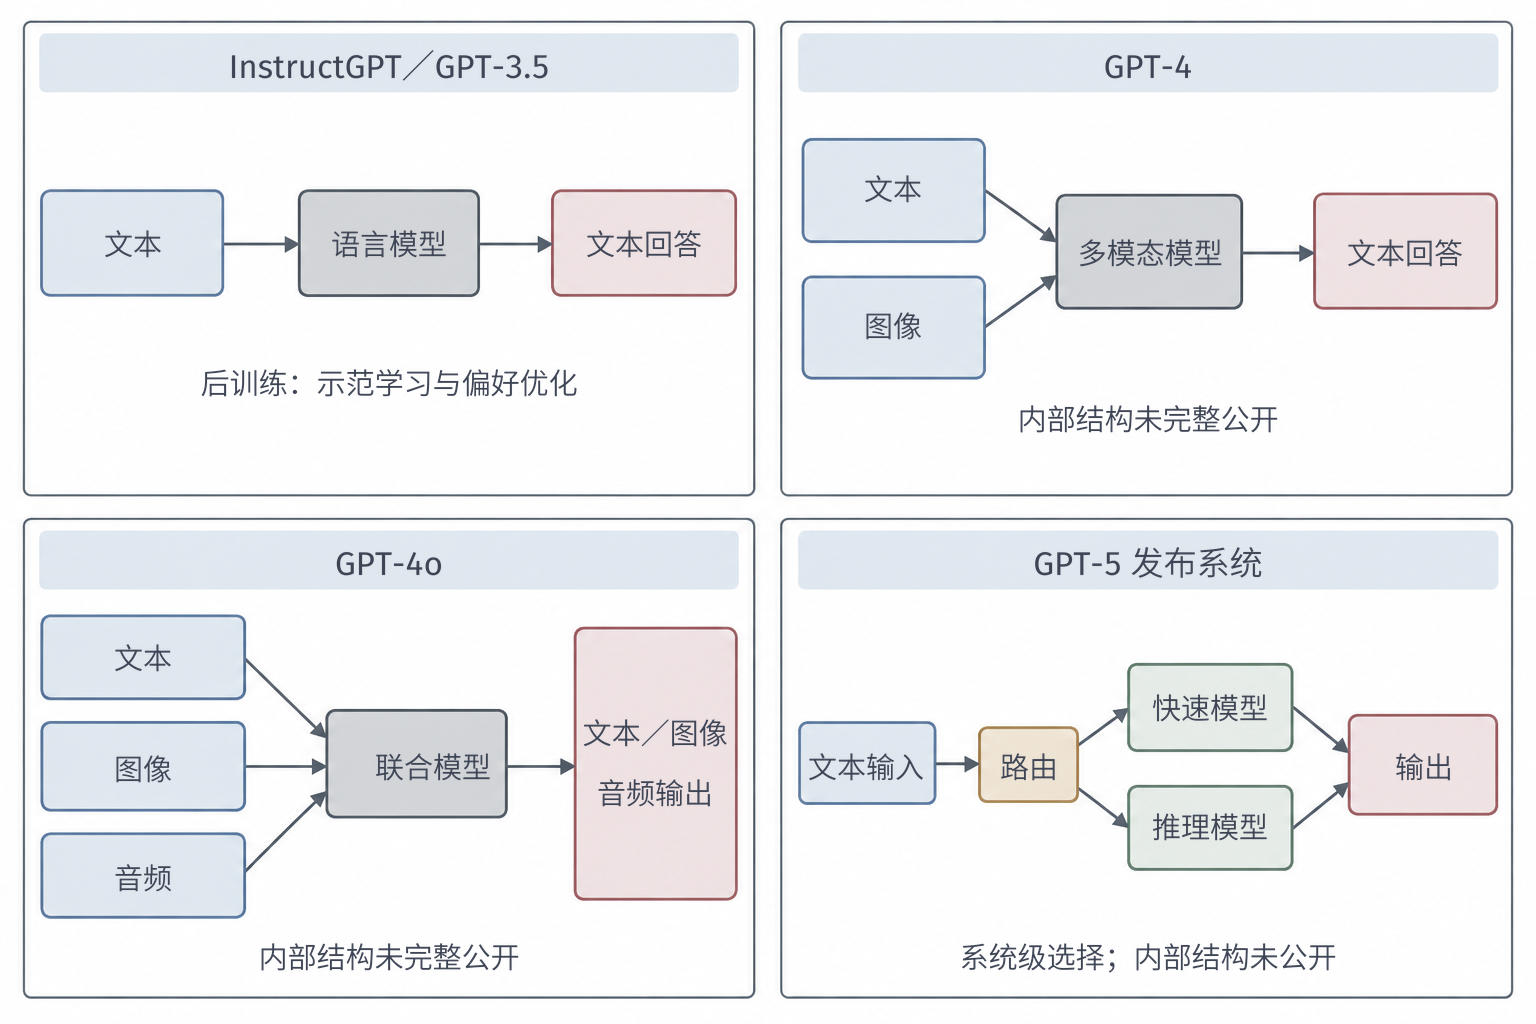
\includegraphics[width=130.048mm]{figures/05-neural-network-models/00-shared/generated/transformer-gpt-public-interfaces/figure.png}
  \caption{GPT后续代表版本的公开接口与系统组织。InstructGPT／GPT-3.5阶段主要改变后训练和交互；GPT-4支持图像与文本输入、文本输出；GPT-4o以文本、视觉、音频端到端联合训练，图示对应模型能力，特定产品功能以各发布阶段的实际开放范围为准；GPT-5发布系统在快速与深入推理模型间路由。灰色模块标明尚未披露的逐层细节，绿色模块仅标示所公开的计算路径。信息依据对应官方报告与发布说明，版本比较截至图中标注的发布阶段。}
  \label{fig:transformer-gpt-public-interfaces}
\end{figure*}

表~\ref{tab:transformer-gpt-generations}将各代变化对应到已经披露的对象。GPT-1至GPT-3可以比较具体块结构与配置；后续公开材料更多描述后训练、模态和系统组织，能够支持的比较也相应有所不同。

\begin{table*}[htbp]
  \centering
  \small
  \begin{tabular}{@{}p{25mm}p{64mm}p{66mm}@{}}
    \toprule
    代表版本 & 已公开的主要变化 & 阅读这些变化时应保留的区别 \\
    \midrule
    GPT-1（2018） & 因果解码器、Post-LN；12层、宽768；语言模型预训练后进行任务微调 & 预训练目标与下游任务监督可以不同 \\
    GPT-2（2019） & 改用Pre-LN并增加末端归一化；最大约15亿参数；1024词元上下文 & 零样本任务提示不需要再训练一个专用输出头 \\
    GPT-3（2020） & 延续Pre-LN；稠密与局部稀疏注意力交替；最大1750亿参数；2048词元上下文 & 提示中的少样本示例不等于梯度微调 \\
    InstructGPT／GPT-3.5阶段（2022） & 人类示范与偏好用于后训练；ChatGPT采用对话交互 & 基座模型、后训练方法和对话产品分属不同层面 \\
    GPT-4（2023） & 图像与文本输入，生成文本；内部架构细节未公开 & 多模态能力不提供确定参数量或专家数的证据 \\
    GPT-4o（2024） & 文本、视觉、音频端到端联合训练 & 模态扩展不能直接还原为一张已知的逐层网络图 \\
    GPT-5发布系统（2025） & 在快速响应与深入推理模型之间路由 & 系统级模型选择不等于层内词元级MoE \\
    \bottomrule
  \end{tabular}
  \caption{GPT家族的代表性演进。参数与上下文数字指相应原论文的配置，GPT-4之后列出官方明确披露的能力或系统组织，不推测未公开的网络细节；表格也不用于比较当前产品的可用性。}
  \label{tab:transformer-gpt-generations}
\end{table*}

\subsubsection{T5：把不同任务组织成文本到文本}

翻译生成另一种语言，分类输出一个类别，摘要输出较短文本；这些任务可以共享“读入条件文本、生成目标文本”的接口。\term{T5}（Text-to-Text Transfer Transformer）使用编码器—解码器，把任务说明和输入交给双向编码器，由因果解码器生成答案并交叉读取条件。它保留原始Transformer的两条路径，但采用相对位置偏置、Pre-LN和简化的归一化；原始基础FFN使用ReLU\scite{raffel2020t5}

T5的代表预训练任务是恢复被删去的连续片段。图~\ref{fig:transformer-architecture-t5}把“猫追狗”变成“猫$\langle S_1\rangle$狗”，解码器生成“$\langle S_1\rangle$追$\langle S_2\rangle$”，并以EOS结束生成。这些专用标记称为\term{哨兵词元}（sentinel token），作用是标明缺失片段及其边界。一个标记可以代替多个连续词元，因此目标长度可以变化。BERT在选中的输入位置恢复词元，T5在目标端串联缺失片段，逐步生成整段恢复内容。

\begin{figure*}[htbp]
  \centering
  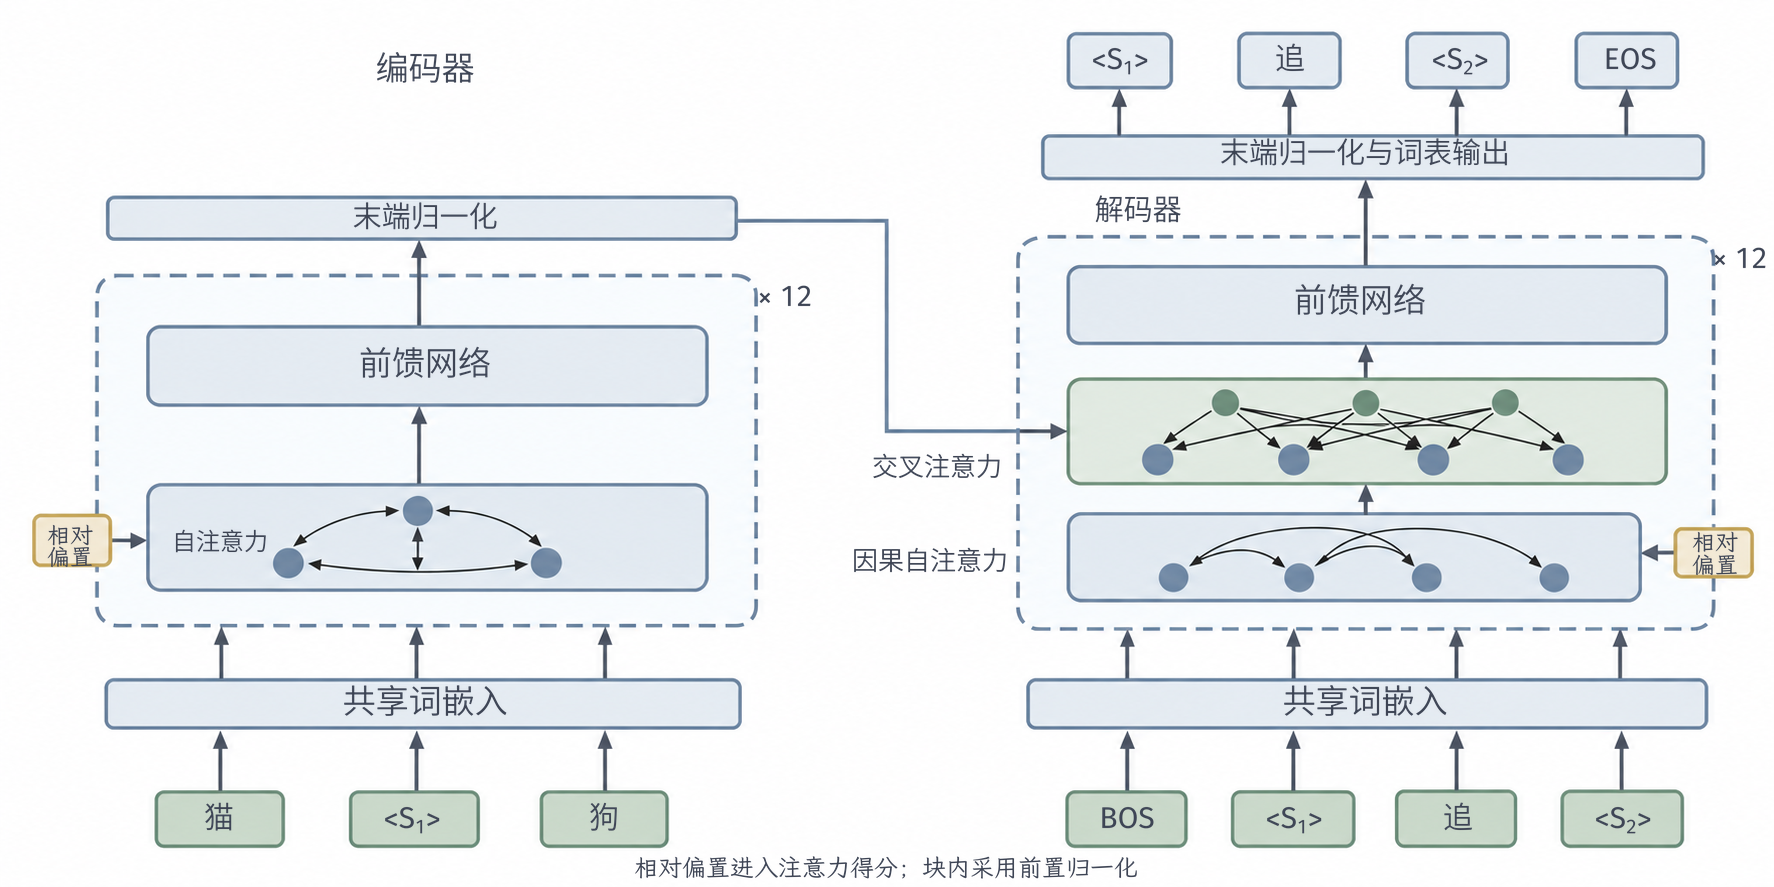
\includegraphics[width=150.199mm]{figures/05-neural-network-models/00-shared/generated/transformer-architecture-t5/figure.png}
  \caption{T5 Base的片段恢复与整网结构。$\langle S_1\rangle$替代源句中的缺失片段，目标中的同名标记引出恢复内容，$\langle S_2\rangle$结束该恢复片段，EOS结束生成。BOS表示解码起始输入。编码器与解码器各堆叠12个块，最终源表示供交叉注意力读取。相对位置偏置加入注意力得分，输入不叠加绝对位置向量。图中显式保留堆叠末端归一化，目标端与词表头合并展示；省略块内入口归一化、残差与Dropout。结构和任务依据Raffel等（2020）。}
  \label{fig:transformer-architecture-t5}
\end{figure*}

恢复目标由被删片段及哨兵标记串联而成，保留的源词元作为条件供解码器读取。给定扰动源句，按式\eqref{eq:transformer-conditional-loss}对恢复序列逐词计算损失；教师强制与因果掩码仍然适用。多处缺失按各哨兵的顺序组织，源长、缺失片段总长和标记数共同决定计算量。其Pre-LN仅按均方根调整尺度，保留可学习缩放，省去均值减除和平移项；本章标准LayerNorm另有这两项操作。

多个缺失片段更能说明哨兵的作用。假设把教学句“猫在院里追狗”中的“在院里”和“狗”分别删去，源端便是“猫$\langle S_1\rangle$追$\langle S_2\rangle$”，目标依次生成“$\langle S_1\rangle$在院里$\langle S_2\rangle$狗$\langle S_3\rangle$”，再输出EOS。源、目标中相同的标记指向同一缺口，最后一个新标记表示已没有后续待恢复片段。解码器只需生成被删内容及边界标记，保留下来的“猫”和“追”继续作为条件参与交叉读取。

这种接口使分类也能写成生成类别文本，任务之间不必各自规定一种输出头；源端双向理解与目标端因果生成的职责保持清楚。相应代价是仍要维护编码器、解码器与交叉注意力，生成式分类还需要规定合法类别词及其读出方式。任务可以复用文本输入输出的训练流程，所需目标长度、合法答案集合和评价量仍由各任务规定。



\subsubsection{架构之间如何取舍}

表~\ref{tab:transformer-common-architectures}将比较标准固定为已知条件、输出过程与结构代价。对一个具体任务，先判断后文何时可见、结果是否需要逐步生成，再选择网络组织。BERT与RoBERTa的主要差异位于预训练方案；原始Transformer与T5共享编码器—解码器组织，却采用不同的位置表示、归一化和任务目标。模型名称还包含训练方案与配置，信息流类型则按允许读取的来源与次序比较。

\begin{table*}[htbp]
  \centering
  \small
  \begin{tabular}{@{}p{24mm}p{34mm}p{47mm}p{50mm}@{}}
    \toprule
    代表模型 & 条件与读取规则 & 结构带来的便利 & 相应代价或使用边界 \\
    \midrule
    原始Transformer & 源双向；目标因果并交叉读取源 & 完整编码源句，生成时复用源表示 & 两组网络和交叉注意力；目标仍逐步产生 \\
    BERT & 扰动输入内双向读取 & 一次形成利用左右语境的各位置表示 & MLM不直接定义自由续写；任务需要适配输出头 \\
    RoBERTa & 与BERT同属双向编码 & 保持结构，改进预训练数据与优化方案 & 预训练投入增大；生成边界与BERT相似 \\
    GPT & 单一路径因果读取 & 前缀与答案共享接口，直接学习逐词生成 & 早期位置不读后文；长输出需要多步解码 \\
    T5 & 条件双向；目标因果并交叉读取条件 & 文本到文本接口统一多种任务 & 双堆栈成本；类别文本等仍需规定读出规则 \\
    \bottomrule
  \end{tabular}
  \caption{代表架构的优势与边界。比较的是信息流和任务接口，不是在不同参数量、训练数据与硬件下比较实测速度或任务分数。同一家族的后续版本还可能修改位置编码、归一化和前馈层。}
  \label{tab:transformer-common-architectures}
\end{table*}

架构规定了可计算的信息路径，训练数据决定模型见过什么，学习目标决定哪些行为受到奖励，解码与系统组织决定模型怎样被调用。这些因素共同构成实际预测过程，各项差异按输入、参数更新和执行步骤分别解释。


\FloatBarrier
\section{参数学习}
\label{sec:transformer-learning}

嵌入、注意力投影、前馈层、归一化和输出层由同一预测目标联合学习。一个批次中的样本可以具有不同有效长度，损失只覆盖监督位置；按样本平均与按词元平均会给予长序列不同权重，相应权重规定了经验目标与后续风险分析中的样本贡献。

在读具体推导前，先明确本节要回答的两个实践问题。第一，训练开始前这些参数应该取多大？Transformer里有多条对尺度特别敏感的路径——内容与位置相加的输入、点积得分、残差流上的逐次累加——初始化若不控制好，第一步的Softmax就可能饱和或让激活爆炸，因此初始化比普通前馈网络更讲究。第二，损失的梯度如何沿注意力这种新运算传回？这里有一条前馈网络里没有的分叉：注意力参数既改变“读出的值内容”，又改变“各位置的读取权重”，反向传播时这两条路径要分别计算后再汇合。本节先讨论初始化，再系统推导注意力与层归一化的导数；优化器、学习率调度及通用正则化由训练与泛化章节展开。

\subsection{参数初始化}
\label{sec:transformer-initialization}

为什么不能沿用单一的初始化方案？因为Transformer里不同参数所处的计算路径，其输出尺度对参数尺度的依赖方式不同，需要分别控制。第\ref{sec:ffn-initialization}节的对称性打破和方差传播原则仍然适用，但Transformer还需同时控制内容嵌入、点积得分与残差流的尺度。输入嵌入可从零均值分布初始化，不同词元独立采样；如果内容项使用$\sqrt d$缩放，初始方差应连同这一缩放考虑。可学习位置表也需要适当尺度，避免输入在尚未学习时被位置项完全主导。连续输入则应先明确量纲和训练数据归一化，再设置投影。

对不带激活的投影$\bm Y=\bm X\bm W$，若输入坐标零均值、方差为$s_x^2$，各权重彼此独立、与输入独立、零均值且方差为$s_w^2$，输入宽度为$d_{\mathrm{in}}$，简化计算给出输出坐标方差$d_{\mathrm{in}}s_w^2s_x^2$。可用Glorot尺度兼顾输入输出宽度，或用与$d_{\mathrm{in}}^{-1}$同阶的方差控制前向尺度；ReLU前馈支路则可采用式\eqref{eq:ffn-he-initialization}的思路。激活、门控和残差参数化会继续改变尺度，投影方差因此按各支路的输入与输出配置。

查询与键的初始尺度直接影响Softmax。若二者每坐标方差分别为$s_q^2,s_k^2$，沿用坐标独立和零均值近似，缩放后点积方差为$s_q^2s_k^2$。因此，除以$\sqrt{d_k}$只抵消宽度因素；过大的投影范数仍会使得分过尖。值与输出投影则决定注意力支路加入残差的大小。FFN的第二次投影也位于残差支路末端，应与第一投影和非线性一起检查输出尺度。

深度增加时，多次相加可能持续放大残差流。若一个简化子层写为$\bm h^{(l)}=\bm h^{(l-1)}+a_l\bm f^{(l)}$，且各增量与已有表示不相关、各坐标方差为$s_f^2$，则增量方差之和为$\sum_l a_l^2s_f^2$。取$a_l$与$L^{-1/2}$同阶可在这个近似下控制累积量；实际分支往往相关，深层训练还需联合考察这些相关性、梯度和归一化位置。缩小支路末端权重、显式残差缩放与可学习门控是不同参数化，后文会比较它们怎样控制新增支路。

归一化的缩放和平移常分别初始化为1和0；输出层按其输入宽度设置尺度。若输入输出共享嵌入，两处梯度会累积到同一参数，初始化也只执行一次。把整个投影都置零可能阻断上游学习：例如$\bm Q=\bm K=\bm0$时，得分对查询和键的局部梯度都为零。特定设计也会把少量支路末端置零。此时可沿计算图确定初始哪些参数有非零导数，以及后续更新怎样打开这些路径。

\subsection{反向传播}
\label{sec:transformer-backpropagation}

注意力的参数既影响“读取什么”，也影响“怎样评分”。理解这一点，就抓住了本节推导的主线：当输出出错时，误差既可以通过“被读出的值”往回传（这个值贡献得多，就该多改它），也可以通过“读取权重”往回传（这个位置读多了，就该调低它的得分）。两条路径在注意力处交汇，必须分别求清。为把两条路径分清，采用矩阵梯度记号$\bm G_{\mathrm X}=\partial\ell/\partial\bm X$，其形状与$\bm X$相同，并以Frobenius内积定义微分$\mathrm d\ell=\langle\bm G_{\mathrm X},\mathrm d\bm X\rangle_{\mathrm F}$。从式\eqref{eq:transformer-attention}中单头的$\bm Z=\bm A\bm V$开始，若下游给出$\bm G_{\mathrm Z}$，则
\begin{equation}
  \bm G_{\mathrm V}=\bm A^{\top}\bm G_{\mathrm Z},\qquad
  \bm G_{\mathrm A}=\bm G_{\mathrm Z}\bm V^{\top}\text{。}
  \label{eq:transformer-aggregation-gradient}
\end{equation}
值梯度汇集所有查询对同一值的读取贡献；权重梯度比较不同值对当前输出变化的作用。固定权重时仍有值梯度；学习读取比例时，还要从权重沿Softmax和评分继续回传。

对第$i$行，把有效权重写为列向量$\bm a_i$。Softmax各权重由共同分母耦合，将其Jacobian与该行权重梯度相乘，得到
\begin{equation}
  (\bm G_{\mathrm S})_{i,j}
   =\bm A_{i,j}\left((\bm G_{\mathrm A})_{i,j}
       -\sum_{t=1}^{n_s}\bm A_{i,t}(\bm G_{\mathrm A})_{i,t}\right)\text{。}
  \label{eq:transformer-softmax-gradient}
\end{equation}
这一求导将本章式\eqref{eq:transformer-softmax-scale-gradient}的局部Jacobian与上游梯度相乘。计算限定在有效集合上，被禁止的权重与得分梯度取零，以避免把无穷掩码当作普通浮点变量求导。每行得分梯度之和为零，与Softmax对整行得分加同一常数不变的性质对应。Softmax的共同分母让各权重相互影响：某个值的梯度要减去当前加权平均作用，才得到该位置的得分梯度。

\Needspace{45mm}
\begin{example}[从聚合误差到评分误差]
  \label{ex:transformer-gradient-numerical}
  沿用示例~\ref{ex:transformer-attention-numerical}未加掩码的情形，令$\ell=(\bm z_2)_2$，即只考察“追”的输出向量的第二坐标，上游梯度为$(0,1)^{\top}$。三个权重的梯度为$0,2,1$，加权平均为$5/4$，得分梯度因此为$-5/16,3/8,-1/16$，总和为零。值梯度则分别为$(0,1/4)^{\top}$、$(0,1/2)^{\top}$和$(0,1/4)^{\top}$。若最小化此目标，评分路径倾向于降低第二个值的权重，值路径还可以直接降低被读取的第二坐标；两种变化共同影响输出。
\end{example}

掩码固定时，对缩放点积继续求导可得
\begin{equation}
  \bm G_{\mathrm Q}=\frac{\bm G_{\mathrm S}\bm K}{\sqrt{d_k}},\qquad
  \bm G_{\mathrm K}=\frac{\bm G_{\mathrm S}^{\top}\bm Q}{\sqrt{d_k}}\text{。}
  \label{eq:transformer-qk-gradient}
\end{equation}
查询梯度聚合相关键，键梯度聚合读取它的查询；固定因果掩码只删除禁止的贡献。若得分还包含可学习位置偏置，相应参数按其使用的所有位置对累积得分梯度。

式\eqref{eq:transformer-qkv}的投影梯度为
\begin{equation}
  \begin{aligned}
    \nabla_{\bm W_{\mathrm q}}\ell&=\bm H_{\mathrm q}^{\top}\bm G_{\mathrm Q},\\
    \nabla_{\bm W_{\mathrm k}}\ell&=\bm H_{\mathrm s}^{\top}\bm G_{\mathrm K},\qquad
    \nabla_{\bm W_{\mathrm v}}\ell=\bm H_{\mathrm s}^{\top}\bm G_{\mathrm V},\\
    \bm G_{\mathrm H_{\mathrm q}}&=\bm G_{\mathrm Q}\bm W_{\mathrm q}^{\top},\\
    \bm G_{\mathrm H_{\mathrm s}}&=\bm G_{\mathrm K}\bm W_{\mathrm k}^{\top}
                      +\bm G_{\mathrm V}\bm W_{\mathrm v}^{\top}\text{。}
  \end{aligned}
  \label{eq:transformer-projection-gradient}
\end{equation}
交叉注意力的两侧接到不同上游模块；自注意力的两侧是同一矩阵，所以查询、键、值三条输入梯度需要相加。加入投影偏置时，其梯度为对应矩阵梯度沿位置求和。共享词元嵌入也按词元编号把各出现位置的贡献相加。

多头输出若为$\bm Y=\bm C\bm W_{\mathrm o}$，则$\nabla_{\bm W_{\mathrm o}}\ell=\bm C^{\top}\bm G_{\mathrm Y}$，$\bm G_{\mathrm C}=\bm G_{\mathrm Y}\bm W_{\mathrm o}^{\top}$。按拼接的列范围拆开$\bm G_{\mathrm C}$，各头分别执行上述求导，再将共同输入的梯度求和。各头分别更新自己的投影，共同输入则接收所有读取分支的梯度和。

残差相加把同一上游梯度送入直接路径和子层路径。对Pre-LN子层$\bm y=\bm x+F(\operatorname{LN}(\bm x))$，列向量记号下有
\begin{equation}
  \bm g_{\mathrm x}=\bm g_{\mathrm y}
     +\bm J_{\operatorname{LN}}^{\top}\bm J_F^{\top}\bm g_{\mathrm y}\text{。}
  \label{eq:transformer-preln-gradient}
\end{equation}
FFN沿用前馈求导。LN的每个输出坐标还依赖本行的均值与方差，输入梯度需要计入这些统计量随输入产生的变化。对式\eqref{eq:transformer-layernorm}的一行输入，先把中心化后的向量和公共分母分别记为
\[
  \bm c=\bm x-\mu\bm1,\qquad
  r=\sqrt{\frac1d\bm c^{\top}\bm c+\varepsilon}
   =\sqrt{s^2+\varepsilon}\text{，}
\]
其中$\mu=\mu(\bm x)$、$s^2=s^2(\bm x)$，且$\bm1^{\top}\bm c=0$、$r>0$。若归一化输出为$\bm y$，令$\widehat{\bm x}=(\bm x-\mu\bm1)/\sqrt{s^2+\varepsilon}=\bm c/r$、$\bm u=\bm g_{\mathrm y}\odot\bm\gamma$，以横线表示坐标平均。求输入梯度时固定$\bm\gamma$和$\bm\beta$，由$\bm y=\bm\gamma\odot\widehat{\bm x}+\bm\beta$可得$\mathrm d\ell=\bm u^{\top}\mathrm d\widehat{\bm x}$；因此$\bm u$就是反传到标准化向量$\widehat{\bm x}$的梯度。

先把$\bm c$视为输入，考察归一化分母的变化。由$r^2=d^{-1}\bm c^{\top}\bm c+\varepsilon$求微分，再对$\widehat{\bm x}=\bm c/r$使用乘积法则，得到
\[
  \mathrm d r=\frac{\bm c^{\top}\mathrm d\bm c}{d\,r},\qquad
  \mathrm d\widehat{\bm x}
    =\frac{\mathrm d\bm c}{r}
       -\frac{\bm c}{r^2}\,\mathrm d r\text{。}
\]
第一项是在分母暂不变化时，$\bm c$直接改变标准化向量的贡献；第二项计入所有坐标通过共同分母$r$产生的影响。把这两个微分代入$\mathrm d\ell$，并收集$\mathrm d\bm c$的系数，得到
\[
  \begin{aligned}
    \mathrm d\ell
      &=\frac{\bm u^{\top}\mathrm d\bm c}{r}
          -\frac{\bm u^{\top}\bm c}{r^2}\,\mathrm d r,\\
    \bm g_{\mathrm c}
      &=\frac{\bm u}{r}
          -\frac{\bm c\,(\bm c^{\top}\bm u)}{d\,r^3}\\
      &=\frac{\bm u-\widehat{\bm x}\,\overline{u\widehat x}}{r}\text{，}
  \end{aligned}
\]
其中$\bm g_{\mathrm c}=\partial\ell/\partial\bm c$，$\overline{u\widehat x}=d^{-1}\sum_{k=1}^d u_k\widehat x_k$是逐坐标乘积的平均。

再把$\bm g_{\mathrm c}$沿中心化运算传到$\bm x$。由于$\mu=d^{-1}\bm1^{\top}\bm x$，均值的变化会从每个坐标中一起减去，因而
\[
  \begin{aligned}
    \mathrm d\bm c
      &=\mathrm d\bm x-\frac1d\bm1\bm1^{\top}\mathrm d\bm x,\\
    \bm g_{\mathrm x}
      &=\bm g_{\mathrm c}-\overline{g_{\mathrm c}}\bm1\text{。}
  \end{aligned}
\]
这里$\overline{g_{\mathrm c}}=d^{-1}\sum_{k=1}^d(\bm g_{\mathrm c})_k$。中心化使$\overline{\widehat x}=0$，所以$\overline{g_{\mathrm c}}=\overline u/r$。代入前式并恢复$r=\sqrt{s^2+\varepsilon}$，得到
\begin{equation}
  \bm g_{\mathrm x}
   =\frac{\bm u-\overline u\bm1
             -\widehat{\bm x}\,\overline{u\widehat x}}
          {\sqrt{s^2+\varepsilon}}\text{。}
  \label{eq:transformer-layernorm-gradient}
\end{equation}
分子中的$-\overline u\bm1$来自减去行均值的反传，$-\widehat{\bm x}\,\overline{u\widehat x}$来自归一化分母随输入变化的反传。两项都在同一行内汇集坐标的作用，没有引入其他位置或样本的统计量；整个推导保留了$\varepsilon$，零方差输入的分母仍为正。
缩放和平移的梯度分别由$\bm g_{\mathrm y}\odot\widehat{\bm x}$和$\bm g_{\mathrm y}$沿位置、样本累积。训练中若使用Dropout，还需按前向使用的同一随机掩码回传。至此，输出损失可以经注意力的读取与评分、逐位置变换和残差路径，传到全部可训练参数；梯度提供参数更新方向，优化进展还取决于目标形状、步长及所用梯度估计。

\FloatBarrier
\section{Transformer的扩展}
\label{sec:transformer-extensions}

标准网络将输入表示、位置读取、特征变换和残差更新组合起来。此后大量研究都在回答同一个现实问题：当序列变得很长、模型变得很大时，标准Transformer的开销吃不消，应该在哪里动手？要在众多方法中不迷失，可以先区分它们改动的是三件不同的东西——读取规则本身（让谁和谁相连、用什么公式打分）、同一次计算的执行与存储方式（数学结果不变，只是算得更省）、以及每个位置内部的特征变换（注意力之外的FFN、归一化和连接）。扩展方法可以改变其中某个计算，也可以只改变同一计算的执行与存储方式。位置关系决定怎样匹配，特征选择决定哪些读取结果进入更新；位置对运算、中间激活及生成缓存又分别消耗计算和存储。扩展方法按这些具体目标调整不同部分。这些目标会影响不同资源，因而可以组合，也可能相互制约。下面依次考察位置编码、注意力、前馈层、归一化、深层连接和混合结构六类扩展，阅读时可不断追问：这个方法改变的到底是“算什么”还是“怎么算”，以及它省下的是计算、显存还是带宽。

\subsection{位置编码的扩展}
\label{sec:transformer-position-extensions}

顺序信息可以加到输入，也可以进入位置对评分。前者给每个位置一个表示，后者让读取直接依赖相对距离；旋转则提供了把位置变换嵌入点积的实现机制。下面固定内容投影，比较位置到底在哪里参与计算。

\subsubsection{绝对位置编码}

可学习位置表$\bm P\in\mathbb R^{n_{\max}\times d}$直接提供式\eqref{eq:transformer-input-position}中的$\bm p_i$，参数量为$n_{\max}d$。位置表只覆盖设定上限，扩充或插值提供新位置向量后，新增长度上的预测还需训练支持或相应外推检验。固定正弦编码对偶数宽度$d$定义
\begin{equation}
  \begin{aligned}
    (\bm p_i)_{2k+1}&=\sin(i\omega_k),\\
    (\bm p_i)_{2k+2}&=\cos(i\omega_k),\qquad
    \omega_k=10000^{-2k/d},
  \end{aligned}
  \label{eq:transformer-sinusoidal-position}
\end{equation}
其中$k=0,\ldots,d/2-1$，向量坐标从1开始，$i$采用本章从1开始的位置编号；改从0开始时需统一输入约定。不同频率使坐标随位置以不同速度变化，无需学习位置表，任意整数位置都可以求值。

图~\ref{fig:transformer-position-waves}把这个变化画成波形。为在同一位置区间内看清快慢，这里取$d=8$，只画$k=0,1$对应的前四个坐标：两对角频率分别为1和0.1弧度／位置。它与图~\ref{fig:transformer-position-example}的四维手算例采用相同公式，但宽度不同；四维例子的第二对频率是0.01，不能把两组参数混用。每对正弦与余弦具有相同周期，彼此相差四分之一周期；高频坐标随位置较快振荡，低频坐标变化较慢。同一横坐标处的各维幅值一起构成该位置向量，每条曲线只提供一个坐标。

\begin{figure}[t]
  \centering
  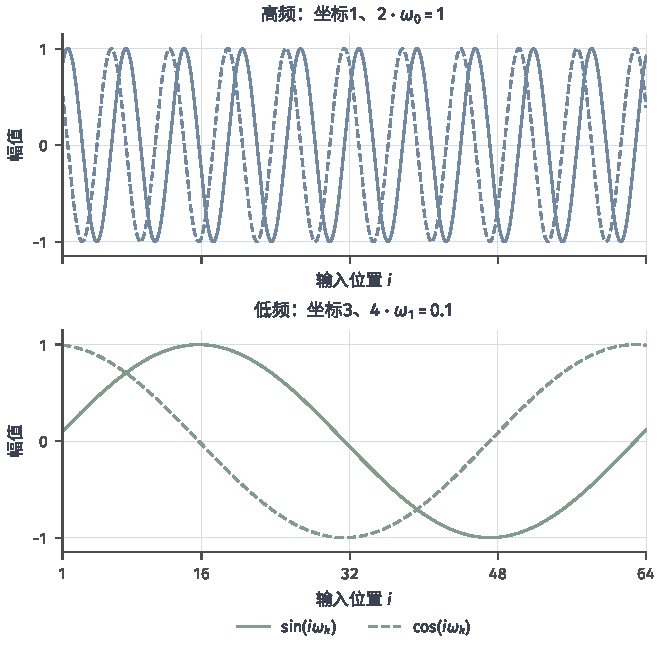
\includegraphics[width=105.412mm]{figures/05-neural-network-models/00-shared/matplotlib/transformer-position-waves/figure.pdf}
  \caption{固定正弦编码中选定坐标随输入位置的变化。取$d=8$，上图为坐标1、2（$k=0$），下图为坐标3、4（$k=1$）；两图横轴范围相同，幅值无量纲。实线为正弦，虚线为同频余弦，周期分别约为6.28和62.83个位置。连续曲线帮助观察波形，实际序列只在整数位置取值；本图仅示意选定维度，不是完整八维编码或训练结果。}
  \label{fig:transformer-position-waves}
\end{figure}

对固定距离$\Delta$，加法公式把$\bm p_{i+\Delta}$写为$\bm p_i$各坐标对的线性变换。这一变换给出位置位移的规律。完整注意力还处理内容投影，所以其得分可以同时依赖内容与位置。把内容和位置相加后，投影点积还包含内容与位置的交叉项；网络需要学习如何使用这些项。新位置向量可以直接求值；训练长度外的预测质量还取决于新上下文与距离如何进入已学计算。

\subsubsection{相对位置向量与距离偏置}

若任务更关心“相隔多远”而非“位于第几位”，绝对位置编码就显得不自然。语言里很多依赖只与相对距离有关（指代、搭配往往出现在邻近位置），与这句话在整篇文章中的绝对位置无关；整段话整体向后平移，词与词的关系应当不变，可每个词的绝对位置编号却全变了。可以直接让位置对得分依赖$j-i$，从而天然具有这种平移不变性。\term{相对位置编码}（relative positional encoding）为位置之间的关系提供表示。设$\bm r_{j-i}^{\mathrm k}\in\mathbb R^{d_k}$、$\bm r_{j-i}^{\mathrm v}\in\mathbb R^{d_v}$为距离对应的键和值修正，则一种形式为
\begin{equation}
  \begin{aligned}
    S_{i,j}&=\frac{\bm q_i^{\top}(\bm k_j+\bm r_{j-i}^{\mathrm k})}
                        {\sqrt{d_k}}+M_{i,j},\\
    \bm z_i&=\sum_j A_{i,j}(\bm v_j+\bm r_{j-i}^{\mathrm v})\text{。}
  \end{aligned}
  \label{eq:transformer-relative-position}
\end{equation}
这里$S_{i,j},M_{i,j},A_{i,j}$是对应矩阵元素的简写，$\bm q_i,\bm k_j,\bm v_j$是各行转置后的向量。键修正改变匹配，值修正把距离信息带入输出。Shaw等采用截断距离，共享过远位置的相对向量；这样限制参数数量，也合并了某些距离差异\scite{shaw2018relative}

若只需修改评分，可以使用标量偏置$b_{j-i}$，将其加到缩放点积上。偏置表可按距离截断或分桶，后者让一组距离共享参数；同一距离只存一个标量时，参数比同距离向量少；它调整评分，向量修正还可以改变匹配方向或输出内容。\term{线性偏置注意力}（attention with linear biases, ALiBi）在因果读取中采用
\begin{equation}
  S_{i,j}^{(a)}=\frac{\bm q_{i,a}^{\top}\bm k_{j,a}}{\sqrt{d_k}}
                 -m_a(i-j),\qquad j\leq i\text{，}
  \label{eq:transformer-alibi}
\end{equation}
其中$m_a>0$是第$a$头的预设斜率，未来位置仍由掩码排除。距离越远，扣除越多；不同斜率提供不同距离偏好。它无需训练长度对应的位置表，原论文在特定语言建模设置中检验了长度外推。这个结果依赖模型、数据与长度范围，线性距离偏好也可能不符合需要精确远距离访问的任务\scite{press2021alibi}

回到“猫／追／狗”，图~\ref{fig:transformer-position-extensions}把相对位置写成可逐格检查的距离矩阵。“追”读取“狗”对应$j-i=1$；若整段句子在更长文本中同时后移5位，距离仍为$8-7=1$。ALiBi进一步把距离变成得分修正：图中“狗”读取三个位置时分别扣除$1.0,0.5,0$，之后才做Softmax。图~\ref{fig:transformer-position-example}是在输入上相加，而这里是在每一对位置的评分上相加，两个操作作用于不同对象。

\begin{figure*}[htbp]
  \centering
  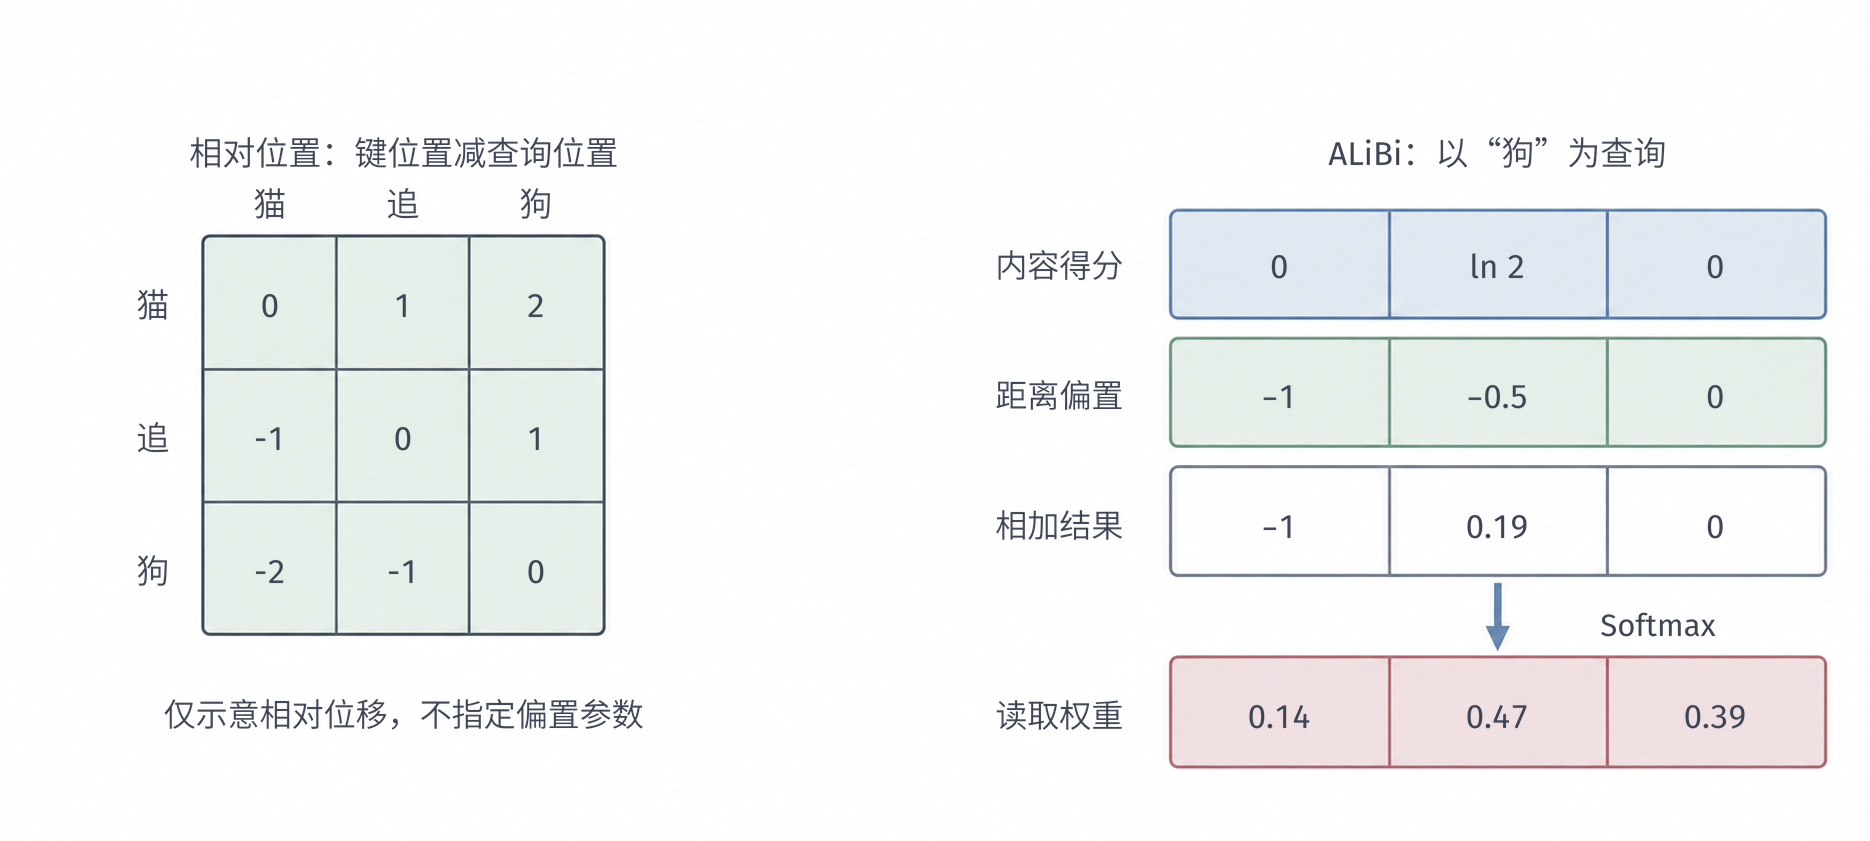
\includegraphics[width=158.327mm]{figures/05-neural-network-models/00-shared/generated/transformer-position-extensions/figure.png}
  \caption{“猫／追／狗”的相对位置。左图行是查询位置$i$、列是键位置$j$，格内为$j-i$，正负号区分左右方向。右图取“狗”为查询、斜率$m=0.5$，演示ALiBi如何修正教学得分并重新归一化；显示数值保留两位小数，真实计算使用未舍入值。}
  \label{fig:transformer-position-extensions}
\end{figure*}

\FloatBarrier
\subsubsection{旋转位置编码}

查询与键怎样变换，决定位置如何进入它们的点积。绝对向量相加会引入内容与位置的交叉项；另一种构造直接控制位置对关系：分别根据位置$i$、$j$变换查询和键，但要求变换后的点积只通过$j-i$依赖位置。\term{旋转位置编码}（rotary position embedding, RoPE）用旋转实现这一要求：位置决定旋转角度，两向量的相对角度进入点积\scite{su2021roformer}

\paragraph{为什么旋转能表示位移}
先考虑二维向量。希望位置每增加1，就施加同一个变换，而且连续移动$i$步再移动$j$步，应等价于移动$i+j$步。平面旋转满足这种组合规律，还能保留向量长度。设每步旋转$\omega$弧度；单位横轴旋转$\theta$后变为$(\cos\theta,\sin\theta)^{\top}$，单位纵轴变为$(-\sin\theta,\cos\theta)^{\top}$。把它们作为两列，就得到
\begin{equation}
  \bm R(\theta)=
  \begin{pmatrix}
    \cos\theta&-\sin\theta\\
    \sin\theta&\cos\theta
  \end{pmatrix}\text{。}
  \label{eq:transformer-rope-rotation}
\end{equation}
对尚未施加本层RoPE旋转的查询$\bm q_i=(q_{i,1},q_{i,2})^{\top}$，令
\[
  \widetilde{\bm q}_i=\bm R(i\omega)\bm q_i
  =\begin{pmatrix}
     q_{i,1}\cos(i\omega)-q_{i,2}\sin(i\omega)\\
     q_{i,1}\sin(i\omega)+q_{i,2}\cos(i\omega)
   \end{pmatrix}\text{；}
\]
键同样取$\widetilde{\bm k}_j=\bm R(j\omega)\bm k_j$。这里旋转的是投影后的查询和键，内容向量仍决定旋转前的方向和长度。

\paragraph{从两个绝对角度推到相对位置}
矩阵转置把旋转角取反。再利用三角函数的和角公式，逐项相乘可得
\begin{equation}
  \begin{aligned}
    \bm R(\alpha)^{\top}&=\bm R(-\alpha),\\
    \bm R(\alpha)\bm R(\beta)&=\bm R(\alpha+\beta),\\
    \bm R(i\omega)^{\top}\bm R(j\omega)
      &=\bm R((j-i)\omega)\text{。}
  \end{aligned}
  \label{eq:transformer-rope-composition}
\end{equation}
令$\Delta=j-i$，代入两向量的点积，有
\begin{equation}
  \begin{aligned}
    \widetilde{\bm q}_i^{\top}\widetilde{\bm k}_j
      &=\bm q_i^{\top}\bm R(\Delta\omega)\bm k_j\\
      &=(q_{i,1}k_{j,1}+q_{i,2}k_{j,2})\cos(\Delta\omega)\\
      &\quad +(q_{i,2}k_{j,1}-q_{i,1}k_{j,2})\sin(\Delta\omega)\text{。}
  \end{aligned}
  \label{eq:transformer-rope-two-dimensional}
\end{equation}
两个内容乘积组合分别乘上余弦和正弦，位置只以$\Delta$出现。若保持内容向量固定，把$i$和$j$同时加上$c$，差值不变，点积也不变。同时平移位置编号保持了这次位置变换；若上下文也改变，旋转前的查询与键会随网络计算改变，完整输出仍可能不同。

图~\ref{fig:transformer-rope}给出可手算的例子。取“追”的位置$i=2$、“狗”的位置$j=3$，并令$\bm q_i=\bm k_j=(1,0)^{\top}$、$\omega=\pi/6$。旋转后
\[
  \begin{aligned}
    \widetilde{\bm q}_i&=(1/2,\sqrt3/2)^{\top},\qquad
    \widetilde{\bm k}_j=(0,1)^{\top},\\
    \widetilde{\bm q}_i^{\top}\widetilde{\bm k}_j
      &=\sqrt3/2=\cos((3-2)\pi/6)\text{。}
  \end{aligned}
\]
两个向量分别转过$60^\circ$和$90^\circ$，点积由$30^\circ$的夹角决定。这里的频率为画图方便而选取；一般内容向量原本就有自己的夹角，旋转在其上叠加位置差带来的角度。

\paragraph{从二维构造完整注意力头}
若$d_k$为偶数，将坐标按$(1,2),(3,4),\ldots,(d_k-1,d_k)$两两配对。第$u$对使用频率$\omega_u=10000^{-2u/d_k}$，其中$u=0,\ldots,d_k/2-1$。把各旋转块放在对角线上，定义
\[
  \bm R_i=\operatorname{diag}\!\left(
    \bm R(i\omega_0),\ldots,\bm R(i\omega_{d_k/2-1})\right)\text{。}
\]
各对坐标独立旋转，完整点积就是它们各自点积之和，因此二维推导逐块成立：
\begin{equation}
  \begin{aligned}
    \widetilde{\bm q}_i&=\bm R_i\bm q_i,\qquad
    \widetilde{\bm k}_j=\bm R_j\bm k_j,\\
    \widetilde{\bm q}_i^{\top}\widetilde{\bm k}_j
      &=\bm q_i^{\top}\bm R_i^{\top}\bm R_j\bm k_j
       =\bm q_i^{\top}\bm R_{j-i}\bm k_j\text{。}
  \end{aligned}
  \label{eq:transformer-rope-relative}
\end{equation}
随后仍按式\eqref{eq:transformer-attention}除以$\sqrt{d_k}$、加掩码并做Softmax。由于$\bm R_i^{\top}\bm R_i=\bm I$，旋转保留查询和键的范数。实现只需逐坐标对计算正弦、余弦和乘加，不必构造稠密的$d_k\times d_k$矩阵；部分坐标也可以保留未旋转形式。这里按相邻坐标配对，其他配对实现则相应重排投影坐标与缓存，保持同一旋转约定。

\paragraph{生成时怎样复用旋转结果}
标准用法旋转查询与键，不旋转值。在后文介绍的KV缓存中，第$t$个位置到来时，只需计算$\widetilde{\bm q}_t=\bm R_t\bm q_t$和$\widetilde{\bm k}_t=\bm R_t\bm k_t$，将旋转后的键与原值$\bm v_t$追加保存。新查询与旧键$\widetilde{\bm k}_j$做点积，式\eqref{eq:transformer-rope-relative}自然给出相对位移$j-t$；已经旋转过的旧键无需再按当前步旋转。词元的逻辑编号决定旋转角度，缓存放在哪个物理地址只决定从哪里读出数值。这种复用要求位置编号、旋转频率与位置缩放规则保持一致；若改变这些规则，旧缓存也需要相应转换或重算。

各频率决定角度随位置改变的速度，单个坐标对的点积可以随距离振荡。例如前述单位向量的得分是$\cos(\Delta\omega)$，这个例子的各次振荡由所取频率决定。RoPE在新位置可以求值，预测仍可能遇到训练未覆盖的相位和距离分布；调整频率或位置尺度会改变读取规律，需要在预期长度范围重新检验。

\begin{figure}[htbp]
  \centering
  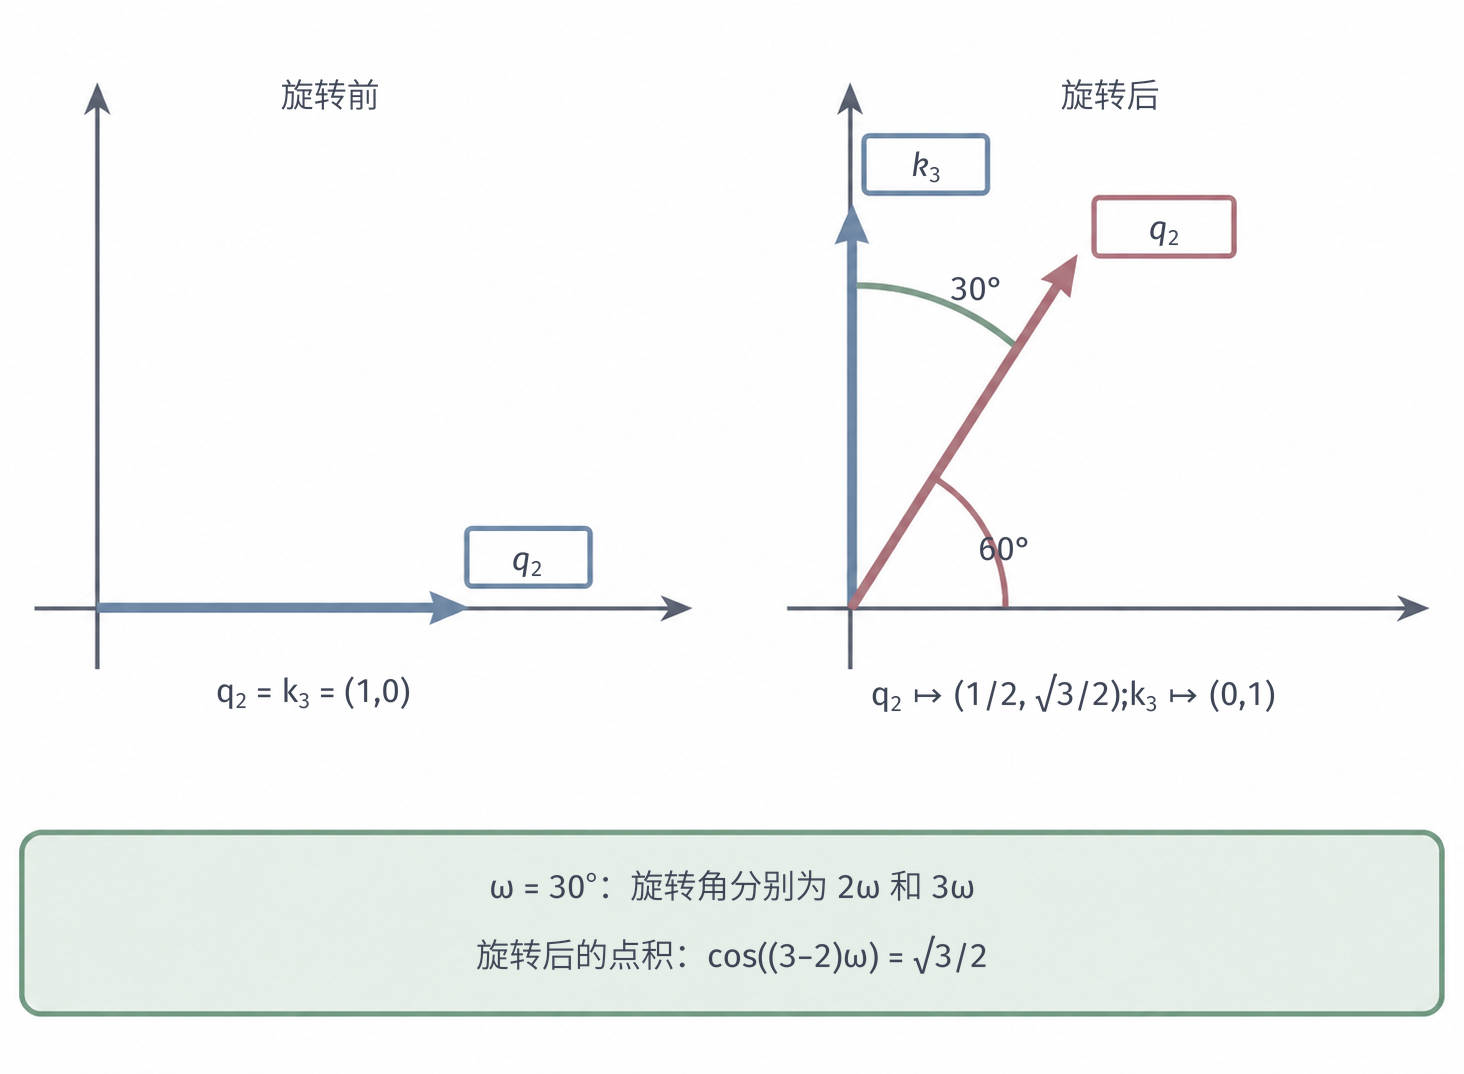
\includegraphics[width=112.000mm]{figures/05-neural-network-models/00-shared/generated/transformer-rope/figure.png}
  \caption{RoPE在一个二维坐标对中的作用。左图两个内容向量重合；右图“追”的查询和“狗”的键按各自位置旋转，夹角为$(3-2)\omega=30^\circ$，点积因此依赖相对位置。示例频率为$\pi/6$，用于演示几何关系；实际模型对多个坐标对采用不同频率，并保留各自的内容向量。}
  \label{fig:transformer-rope}
\end{figure}

绝对与相对描述的是位置关系，旋转描述的是注入机制，一个按绝对编号执行的旋转，可以在点积中形成相对距离关系。可学习绝对表有显式长度参数，固定正弦和RoPE无需位置表，距离偏置由距离覆盖或斜率决定参数量；位置计算的资源与覆盖范围可以据此比较，训练长度外的误差则还需要任务和数据条件。图像还需要保留二维位置，连续时间数据需要处理实际时间间隔，单一序列编号未必足够。



\subsection{注意力机制的扩展}
\label{sec:transformer-attention-extensions}

先看增量生成时一个朴素实现会浪费什么。逐词生成时，每产生一个新词，都要让它去读取此前所有位置；若每一步都把整个前缀重新跑一遍注意力，前面那些早已算过、且不会再变的键和值就被反复重算。\term{键值缓存}（key--value cache, KV cache）保存每层已有位置的键和值，生成时只计算新位置的投影并追加，避免这种重复。固定参数、位置编号和因果掩码时，旧位置表示不依赖未来输入，所以其键值可以复用；如果前缀内容或可见规则改变，原缓存未必继续有效。

对$L$层、$h$头、每头$d_k=d_v$、当前长度$n$的单序列，标准缓存有$2Lnhd_k$个元素，字节量还要乘以每元素的存储字节数和批量大小。旧位置的投影与网络块结果可直接复用，新查询则继续读取$n$个键和值，其位置对算术量为$O(nhd_k)$。将长度从1生成到$n$时，稠密注意力累计仍有平方量级的位置对读取。预填充（prefill）是一次处理已知前缀并建立缓存，逐步解码（decoding）则复用缓存产生后续内容；两者的并行规模和存储瓶颈不同。

\subsubsection{模型效果：信息范围与特征选择}

\paragraph{支持不同信息来源与可见范围}

交叉注意力改变键值来源，因果注意力改变允许的连接，两者可以同时出现于同一目标块。还有一种常见情形介于两者之间：条件生成时，已知的提示或源前缀可以放心地彼此双向读取（它是完整给定的），但正在生成的目标只能读此前内容、不能反向污染条件。\term{前缀注意力}（prefix attention）让给定条件前缀内部互相读取，而目标位置读取前缀和此前目标；前缀表示只由条件前缀形成；若加入目标信息，原来的前缀表示便会改变，需要重新编码。图~\ref{fig:transformer-masks}固定“猫／追／狗／EOS”四个位置，对比三种掩码。前缀方案把“猫追”设为已知条件，两位置内部可以互读；生成“狗”时可以读取这段条件，而“狗”的信息不能反向进入已缓存的条件表示。掩码将条件输入与生成前缀的可见范围直接写入每层计算。

\begin{figure*}[htbp]
  \centering
  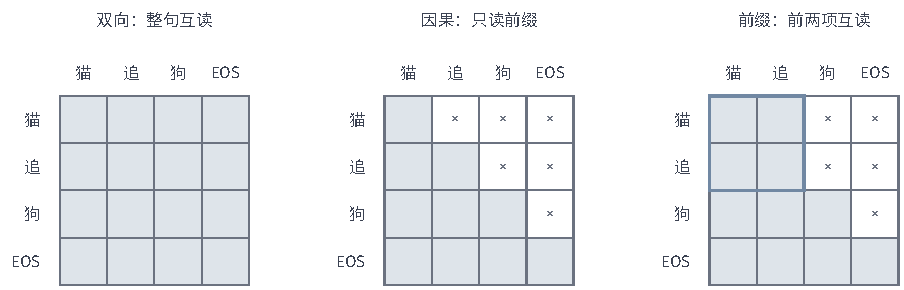
\includegraphics[width=153.003mm]{figures/05-neural-network-models/00-shared/tikz/transformer-masks/figure.pdf}
  \caption{四个位置的读取范围。行表示查询位置$i$，列表示键位置$j$，着色格允许读取，带叉白格禁止读取。左为全部有效输入间的双向读取，中为$j\leq i$的因果读取，右为前两个位置构成条件前缀的读取：前缀内部双向，目标读取全部前缀与截至当前位置的目标输入。目标输入已移位，因此读取当前输入不等于读取当前待预测标签。}
  \label{fig:transformer-masks}
\end{figure*}

\paragraph{优化动态信息选择：门控注意力}

Softmax每行必须把总权重1分配给可见值，即使这些值都不适合当前更新——它只能在候选之间做“相对取舍”，无法表达“这次谁都不值得读、干脆什么都不取”。要获得这种整体开关能力，需要在注意力之外再加一个不被归一化为1的控制量。\term{门控注意力}（gated attention）增加一个输入相关的控制量，调节特征或聚合结果的通过程度。例如，对第$a$头在位置$i$的结果，可以令
\begin{equation}
  \bm g_{i,a}=\sigma(\bm W_{\mathrm g,a}^{\top}\bm h_i+\bm b_{\mathrm g,a}),\qquad
  \widetilde{\bm z}_{i,a}=\bm g_{i,a}\odot\bm z_{i,a}\text{，}
  \label{eq:transformer-gated-attention}
\end{equation}
其中$\bm W_{\mathrm g,a}\in\mathbb R^{d\times d_v}$，Sigmoid门与头输出同宽。每头一个标量门则把整头共同缩放。注意力权重选择“从哪些位置读取”，输出门决定“这次读取的哪些特征应通过”，两者作用对象不同。

门也可置于值投影之后或最终输出投影之后，这些位置通常不等价。值门改变不同来源的内容，查询相关的输出门改变接收端结果。Qiu等比较了门的位置和粒度，并在所测试的大语言模型配置中观察到聚合后Sigmoid门对训练与表示行为的改善；观察到的改进对应论文中的训练配置，其作用范围由模型、目标及数据确定。逐坐标门增加非线性和参数，也要考虑饱和造成的梯度减弱\scite{qiu2025gated}

图~\ref{fig:transformer-gated-attention}接着使用“追”的聚合结果$(0.5,1.25)^{\top}$。若当前表示生成的门为$(0.2,0.8)^{\top}$，逐坐标相乘得到$(0.1,1.0)^{\top}$，分别保留第一维的20\%与第二维的80\%。位置权重在此前已经完成归一化，门按坐标调整混合后的特征，来源位置的权重仍由前面的Softmax给出。标准点积和键值存储都已在门控前完成，其成本继续保留。

\begin{figure*}[htbp]
  \centering
  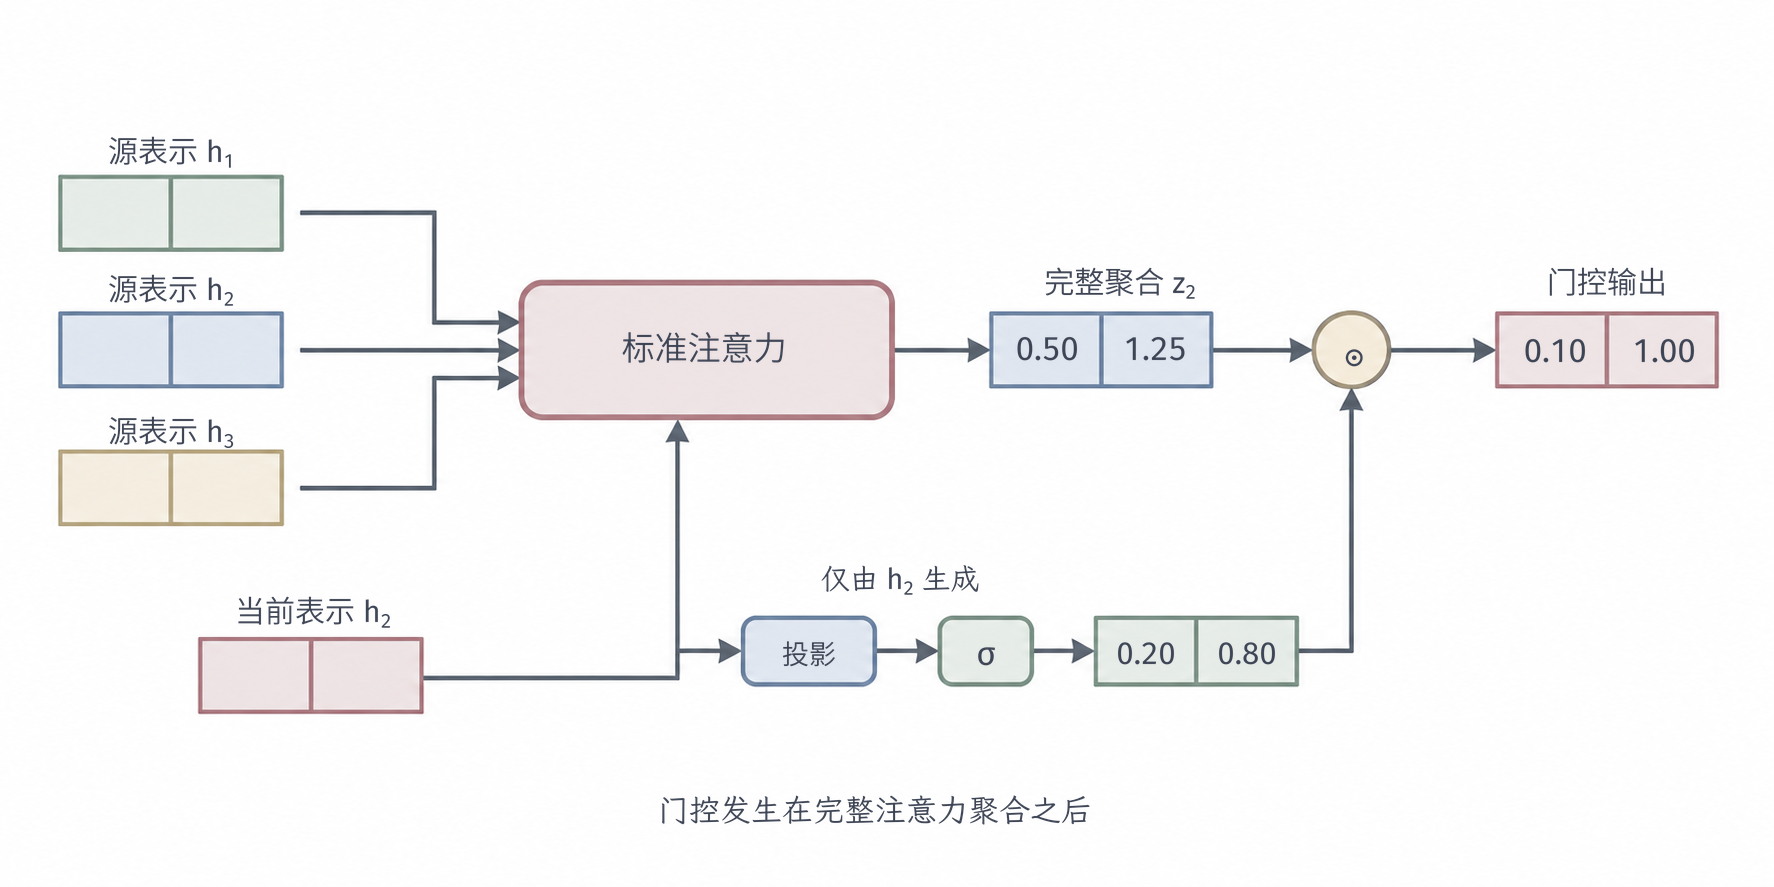
\includegraphics[width=150.199mm]{figures/05-neural-network-models/00-shared/generated/transformer-gated-attention/figure.png}
  \caption{以“追”为查询的聚合后门控。左支路从整段序列读取内容，右支路仅由当前词元表示产生Sigmoid门。教学数值中，聚合结果$(0.5,1.25)$与门$(0.2,0.8)$逐坐标相乘，得到$(0.1,1.0)$。门控制的是输出特征，而不是三个来源位置的概率；图中固定一个头并省略头索引、多头拼接和输出投影，数值并非训练测量。}
  \label{fig:transformer-gated-attention}
\end{figure*}

\subsubsection{训练效率：位置交互与中间存储}

整段训练需要为位置对评分，还要为反向保存或重算中间量。标准稠密注意力的开销主要压在两处：一是$n^2$量级的位置对算术，二是那个$n\times n$得分／权重矩阵带来的中间存储与显存搬运。针对它们，研究上形成了思路清晰的几条路线——直接删掉用不上的连接（稀疏）、换掉Softmax核从而改变求和次序（线性）、把$n$个位置压成少数几个汇总槽（低秩），以及数学结果不变、只优化存储搬运方式（FlashAttention）。连接数影响前一成本，聚合公式与执行方式影响后者及其访存；下面分别说明这些改动在训练和推理中的适用范围。

\paragraph{降低位置连接的计算量：稀疏注意力}

\term{稀疏注意力}（sparse attention）只计算保留的连接。它的依据是一个经验观察：对很多任务而言，真正有用的位置对并不是全部$n^2$个——一个词通常主要依赖邻近的词，再加上少数几个全局关键位置；既然如此，大量远距离连接的权重本来就接近零，为它们付出计算并不划算。例如每个位置读取$w$个窗口位置，再加少量全局位置，若各头保留连接总数为$e_{\mathrm{att}}$，评分和聚合需要$O(e_{\mathrm{att}}(d_k+d_v))$算术操作，权重存储为$O(e_{\mathrm{att}})$。窗口大小和全局连接数固定时，连接数随$n$线性增长；窗口若随$n$增长，复杂度也相应保留窗口长度因子。Sparse Transformer采用特定稀疏分解，使连接数达到$O(n\sqrt n)$量级，其稀疏连接仍多于固定窗口的线性规模$O(n)$\scite{child2019sparse}

删除连接也改变传播范围。只有窗口连接时，一层无法读取窗口之外的信息，跨层传播可扩大范围，却增加依赖路径长度；全局位置使远处信息有较短通路，但也可能形成汇总瓶颈。保留哪些连接决定哪些证据能够到达目标位置，相同比例的稀疏模式也可能形成不同通路。

\paragraph{降低聚合计算量：线性注意力}

\term{线性注意力}（linear attention）把位置对核改写为有限维特征内积，以改变聚合次序。它的关键想法是一条代数恒等式带来的计算次序重排：标准注意力必须先算好每一对（查询，键）的权重，再对值求和，因而绕不开$n^2$个位置对；若相似度能写成“查询特征”和“键特征”的内积，就可以利用结合律先把所有键和值汇总成一份与查询无关的状态，再让每个查询去读这份状态，从而把成本降到对$n$线性。它仍按归一化的成对相似度读取值，但将相似度写成查询特征与键特征的内积。设$\phi:\mathbb R^{d_k}\to\mathbb R^r$，其中$\phi$表示查询和键的特征映射，定义
\[
  \kappa(\bm q,\bm k)=\phi(\bm q)^{\top}\phi(\bm k)\text{。}
\]
要求每个允许读取的位置对都有$\kappa(\bm q_i,\bm k_j)\geq0$，并且每个参与计算的查询至少有一个允许键满足$\kappa(\bm q_i,\bm k_j)>0$。前一个条件使归一化权重非负，后一个条件使分母严格为正。

特征映射需要具体选择。例如，取$r=d_k$，对输入向量$\bm x\in\mathbb R^{d_k}$的第$u$个坐标定义
\[
  [\phi(\bm x)]_u=
  \begin{cases}
    x_u+1,&x_u\geq0,\\
    \exp(x_u),&x_u<0\text{。}
  \end{cases}
\]
这一映射的各坐标均为正，因此任意两个有限输入的特征内积都为正；只要可读键集合非空，分母便为正。这里选择了新的相似度，并未把它声明为原来指数点积相似度的恒等改写。

先考虑各查询都能读取全部$n$个键的情形。第$i$个查询对位置$j$的归一化权重以及读取结果为
\[
  \begin{aligned}
    \bm A^{\mathrm{lin}}_{i,j}
      &=\frac{\kappa(\bm q_i,\bm k_j)}
                   {\sum_{t=1}^n\kappa(\bm q_i,\bm k_t)},\\
    \bm z_i^{\top}
      &=\sum_{j=1}^n\bm A^{\mathrm{lin}}_{i,j}\bm v_j^{\top}\text{。}
  \end{aligned}
\]
这与前面的读取结构相同：先把当前位置对各键的相似度归一化，再按这些权重合成值向量。改变的是相似度的计算形式。将特征内积代入，可以看到为什么不必先保存全部位置对权重：
\[
  \begin{aligned}
    \bm z_i^{\top}
      &=\frac{\sum_{j=1}^n
                  [\phi(\bm q_i)^{\top}\phi(\bm k_j)]\bm v_j^{\top}}
                   {\sum_{j=1}^n\phi(\bm q_i)^{\top}\phi(\bm k_j)}\\
      &=\frac{\phi(\bm q_i)^{\top}
                     \left(\sum_{j=1}^n\phi(\bm k_j)\bm v_j^{\top}\right)}
                   {\phi(\bm q_i)^{\top}
                     \left(\sum_{j=1}^n\phi(\bm k_j)\right)}\text{。}
  \end{aligned}
\]
对固定查询$i$，$\phi(\bm q_i)$不随求和下标$j$变化，所以可以利用分配律和矩阵乘法的结合律，将它提出求和。分子内先累加每个键特征与对应值的外积，分母内先累加键特征；这两份和都不依赖当前查询，可以供不同查询复用。将它们分别记为$\bm T$和$\bm b$，便得到
\begin{equation}
  \begin{aligned}
    \bm T&=\sum_{j=1}^n\phi(\bm k_j)\bm v_j^{\top},\qquad
    \bm b=\sum_{j=1}^n\phi(\bm k_j),\\
    \bm z_i^{\top}&=\frac{\phi(\bm q_i)^{\top}\bm T}
                           {\phi(\bm q_i)^{\top}\bm b}\text{。}
  \end{aligned}
  \label{eq:transformer-linear-attention}
\end{equation}
$\bm T\in\mathbb R^{r\times d_v}$和$\bm b\in\mathbb R^r$先汇总键值，再被所有查询读取。除特征映射和输入输出投影外，单头算术量为$O(nrd_v+nr)$，中间汇总存储为$O(rd_v+r)$；固定$r,d_v$时，这里的成本对$n$线性；特征映射和归一化仍使输出可以是输入的非线性函数。保存所有位置的激活和训练梯度还需额外存储。

因果读取把上述和限制到$j\leq i$，得到$\bm T^{(i)}=\bm T^{(i-1)}+\phi(\bm k_i)\bm v_i^{\top}$、$\bm b^{(i)}=\bm b^{(i-1)}+\phi(\bm k_i)$。它可用固定大小的状态逐步生成，也可在整段输入上做前缀扫描。Katharopoulos等给出了这类计算与循环形式的联系；有限维特征核使聚合次序可以交换；标准Softmax一般需要相应近似，或者由另一种核替代\scite{katharopoulos2020linear}

\paragraph{压缩位置交互表示：低秩注意力}

\term{低秩注意力}（low-rank attention）用较小的交互表示代替全部位置。它的直觉是：一段序列里真正彼此不同、需要分别保存的“信息要点”通常远少于位置数，大量位置携带的是相近或冗余的信息；既然如此，可以先把$n$个键值压缩成少数几个汇总槽，让查询只和这几个槽交互，把$n\times n$降为$n\times r$。例如Linformer在位置维上用$\bm E_{\mathrm k},\bm E_{\mathrm v}\in\mathbb R^{r\times n}$分别压缩键和值，形成$\overline{\bm K},\overline{\bm V}$，再计算$n\times r$的注意力。固定各头配置时，位置压缩、评分和聚合的量级可降为$O(nr(d_k+d_v))$。它依赖低秩近似是否适合输入，并改变了可读取的表示\scite{wang2020linformer}

压缩槽若含未来键值，查询读到这个槽时也会间接读到未来；槽之间的三角掩码无法拆开已混合内容。因果方案需要在压缩阶段就限制信息范围。压缩矩阵还可能绑定最大长度，$r$若为保持精度随$n$增长，实际复杂度也随之改变。删连接限制位置通路，换核限制匹配形式，压缩槽限制被读取表示。相同任务和有效长度使这些取舍能够对应到共同误差与成本。

\begin{figure*}[htbp]
  \centering
  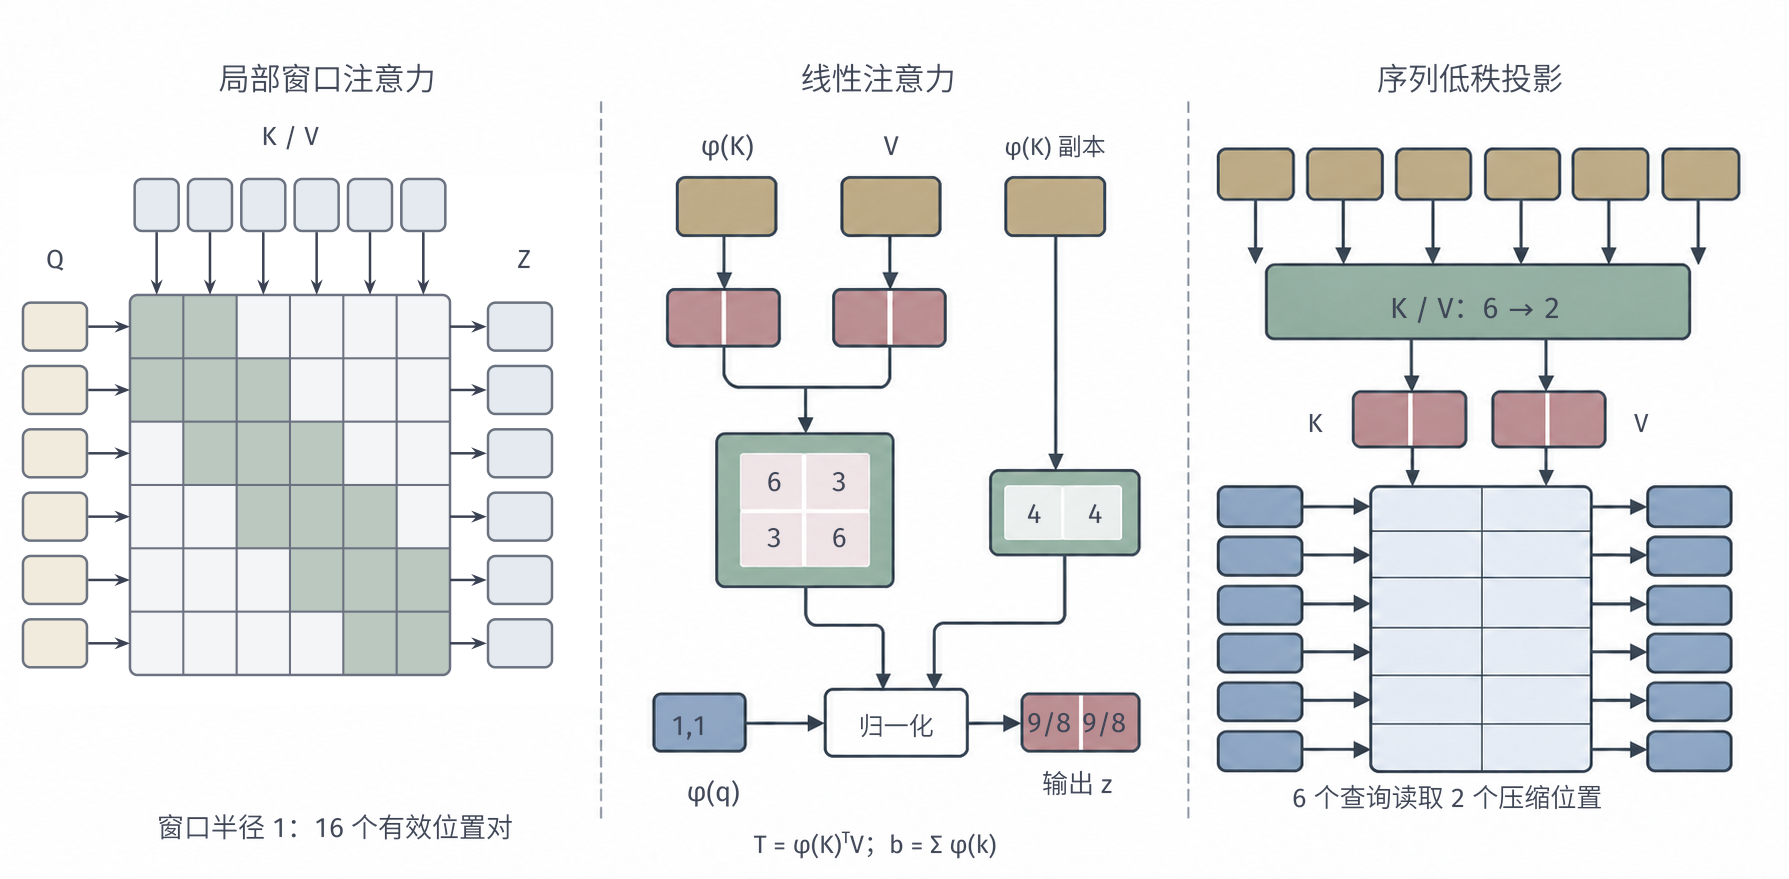
\includegraphics[width=151.469mm]{figures/05-neural-network-models/00-shared/generated/transformer-efficient-attention/figure.png}
  \caption{三条效率路线的具体读法，六个位置可按正文的“猫／在／院／里／追／狗”教学序列理解。左图中查询$\bm Q$对应各行，键值$\bm K/\bm V$对应各列，输出$\bm Z$逐行引出；着色格保留相邻位置的连接，白格表示删除的连接。中图给定教学键特征和值后，先累加外积和特征，再对查询归一化，数值由式\eqref{eq:transformer-linear-attention}复核。右图的示例投影把6个位置压成2个槽，右侧每行表示一个查询对两槽评分，颜色只表示存在连接。所有数值及压缩权重均为教学设定；三种方法并非对同一Softmax结果的等价改写。}
  \label{fig:transformer-efficient-attention}
\end{figure*}

图~\ref{fig:transformer-efficient-attention}把三条路线放回同一句“猫在院里追狗”，按字分成6个位置。左侧局部连接只保留当前位置及其左右邻居，把36个位置对减到16个；“追”这一行可以读取“里、追、狗”，却不能在本层直接读取“猫”。中间线性路线为键特征和值设置可手算的二维数值。

具体取$d_k=r=d_v=2$，依次给出六个位置的键特征和值：
\[
  \begin{array}{ccll}
    j&\text{词元}&\phi(\bm k_j)^{\top}&\bm v_j^{\top}\\
    1&\text{猫}&(1,\tfrac12)&(2,-1)\\
    2&\text{在}&(1,\tfrac12)&(2,-1)\\
    3&\text{院}&(\tfrac12,1)&(-1,2)\\
    4&\text{里}&(\tfrac12,1)&(-1,2)\\
    5&\text{追}&(\tfrac12,\tfrac12)&(3,3)\\
    6&\text{狗}&(\tfrac12,\tfrac12)&(3,3)
  \end{array}
\]
这些是教学设定的特征映射后键向量与投影后值向量，不是训练测量。例如，前面给出的特征映射将$\bm k_1=(0,-\log2)^{\top}$变为$(1,1/2)^{\top}$。要求非负的是成对相似度，值向量的坐标可以为负。

每一行分别贡献一个$2\times2$外积，按六个位置的顺序相加为
\[
  \begin{aligned}
    \bm T
      &=\begin{pmatrix}2&-1\\1&-1/2\end{pmatrix}
        +\begin{pmatrix}2&-1\\1&-1/2\end{pmatrix}\\
      &\quad+\begin{pmatrix}-1/2&1\\-1&2\end{pmatrix}
        +\begin{pmatrix}-1/2&1\\-1&2\end{pmatrix}\\
      &\quad+\begin{pmatrix}3/2&3/2\\3/2&3/2\end{pmatrix}
        +\begin{pmatrix}3/2&3/2\\3/2&3/2\end{pmatrix}\\
      &=\begin{pmatrix}6&3\\3&6\end{pmatrix}\text{。}
  \end{aligned}
\]
键特征也按同一位置顺序逐坐标累加：
\[
  \bm b=
  \begin{pmatrix}
    1+1+\tfrac12+\tfrac12+\tfrac12+\tfrac12\\
    \tfrac12+\tfrac12+1+1+\tfrac12+\tfrac12
  \end{pmatrix}
  =\begin{pmatrix}4\\4\end{pmatrix}\text{。}
\]
六项外积累加为$\bm T=\bigl[\begin{smallmatrix}6&3\\3&6\end{smallmatrix}\bigr]$，键特征相加为$\bm b=(4,4)^{\top}$；查询特征$(1,1)^{\top}$因而得到$(9/8,9/8)^{\top}$。具体地，$\bm T$的两行分别汇总两个键特征坐标对值的两个坐标的贡献；查询特征$(1,1)^{\top}$将两行相加，分子为$(9,9)$，分母为$(1,1)\bm b=8$，所以
\[
  \bm z_i^{\top}
    =\frac{(1,1)\bm T}{(1,1)\bm b}
    =\frac{(9,9)}8
    =(9/8,9/8)\text{。}
\]

也可以回到逐位置权重核对同一结果。该查询与前四个键的相似度均为$3/2$，与后两个键的相似度均为1，总和为8，因此权重依次为$3/16,3/16,3/16,3/16,1/8,1/8$。按这六个权重读取原值，得到
\[
  \begin{aligned}
    \bm z_i
      &=\frac3{16}\left[
          \begin{pmatrix}2\\-1\end{pmatrix}
         +\begin{pmatrix}2\\-1\end{pmatrix}
         +\begin{pmatrix}-1\\2\end{pmatrix}
         +\begin{pmatrix}-1\\2\end{pmatrix}\right]\\
      &\quad+\frac18\left[
          \begin{pmatrix}3\\3\end{pmatrix}
         +\begin{pmatrix}3\\3\end{pmatrix}\right]
       =\begin{pmatrix}9/8\\9/8\end{pmatrix}\text{。}
  \end{aligned}
\]
输出的两维对应值向量的两个特征坐标，不是两个位置的概率；本例两维恰好相等，来自这组六行教学数值的对称设置。逐位置计算相似度并按同一查询的总相似度归一化，再对值加权，与先汇总$\bm T,\bm b$再读取给出相同结果。这里各位置共同贡献一个固定大小的状态，查询再从状态读取。

右图则直接压缩位置：教学投影把前三个位置、后三个位置分别取平均，形成两个键值槽。所有6个查询仍各有一行，但每行只向两个槽评分。图中为便于核对令$\bm E_{\mathrm k}=\bm E_{\mathrm v}=\bm E$；Linformer的投影可以学习，也不必采用局部平均。这三幅图分别改变连接、核与可读取的表示，矩阵缩小分别来自删连接、改变核或合并位置，三个输出由各自的新计算定义。



\paragraph{优化中间存储与访存：FlashAttention}

前面三条路线改变了读取规则或公式，因而都是在“算什么”上做近似或取舍。还有一种浪费与此不同：即使要算的就是标准稠密注意力，把完整的$n\times n$得分、概率矩阵都写进显存、再读回来做加权，本身就耗费大量时间——GPU的算力往往不是瓶颈，数据在显存和计算单元之间来回搬运才是。\term{FlashAttention}保留标准稠密注意力的数学结果，通过分块计算和在线归一化，避免把完整得分、概率矩阵写入大容量显存。它在容量较小的片上存储中反复处理查询和键值块，减少完整中间矩阵的显存读写；反向传播按需要重算部分块，保存的统计量支持恢复这些局部计算\scite{dao2022flashattention}

理解在线Softmax可以只看一个查询。已处理的键集合上，维护最大得分$m$、归一化分母$s=\sum_j\exp(S_j-m)$和未归一化输出$\bm u=\sum_j\exp(S_j-m)\bm v_j$。新键块集合为$B$，块内最大值为$m_B$，更新为
\begin{equation}
  \begin{aligned}
    m'&=\max(m,m_B),\qquad c=\exp(m-m'),\\
    s'&=cs+\sum_{j\in B}\exp(S_j-m'),\\
    \bm u'&=c\bm u+\sum_{j\in B}\exp(S_j-m')\bm v_j\text{。}
  \end{aligned}
  \label{eq:transformer-online-softmax}
\end{equation}
旧统计乘以$c$，是在新最大值下重新表达同一批指数。遍历全部有效块后，输出为$\bm u/s$。初始为空时直接用第一个非空有效块建立统计，避免在全被掩码的块上做$-\infty-(-\infty)$。

沿用示例~\ref{ex:transformer-attention-numerical}，先处理得分$0,\log2$，得到$m=\log2$、$s=3/2$、$\bm u=(1/2,2)^{\top}$；再加入得分0和值$(1,1)^{\top}$，得到$s'=2$、$\bm u'=(1,5/2)^{\top}$，仍输出$(1/2,5/4)^{\top}$。分块没有把不同块分别归一化后简单求和，而是维护全局共同分母。

在固定头数和宽度下，FlashAttention把需要保存的注意力中间量从平方规模降到线性规模，实际训练还需保存其他模块激活。稠密位置对仍然存在，算术量仍为$O(n^2d)$；浮点运算顺序改变，结果可能有舍入差异。这里的“精确”指保留原稠密注意力公式，浮点舍入按实际执行顺序发生。速度收益依赖块大小、硬件和输入形状，其加速针对数据搬运与存储，位置对算术阶数保持原样。

图~\ref{fig:transformer-flashattention}对比“保存整个中间矩阵”与“算完一块就合并”。左侧常规路径显式形成完整得分与概率矩阵，右侧分块路径维护同一组$m,s,\bm u$，跨块更新使最终分母覆盖所有键；旧统计按新最大值重新缩放后，新旧键共同进入同一分母。对其他查询块重复这一过程，就能得到完整输出，而无需让完整得分、概率矩阵在大容量显存中落地。

\begin{figure*}[htbp]
  \centering
  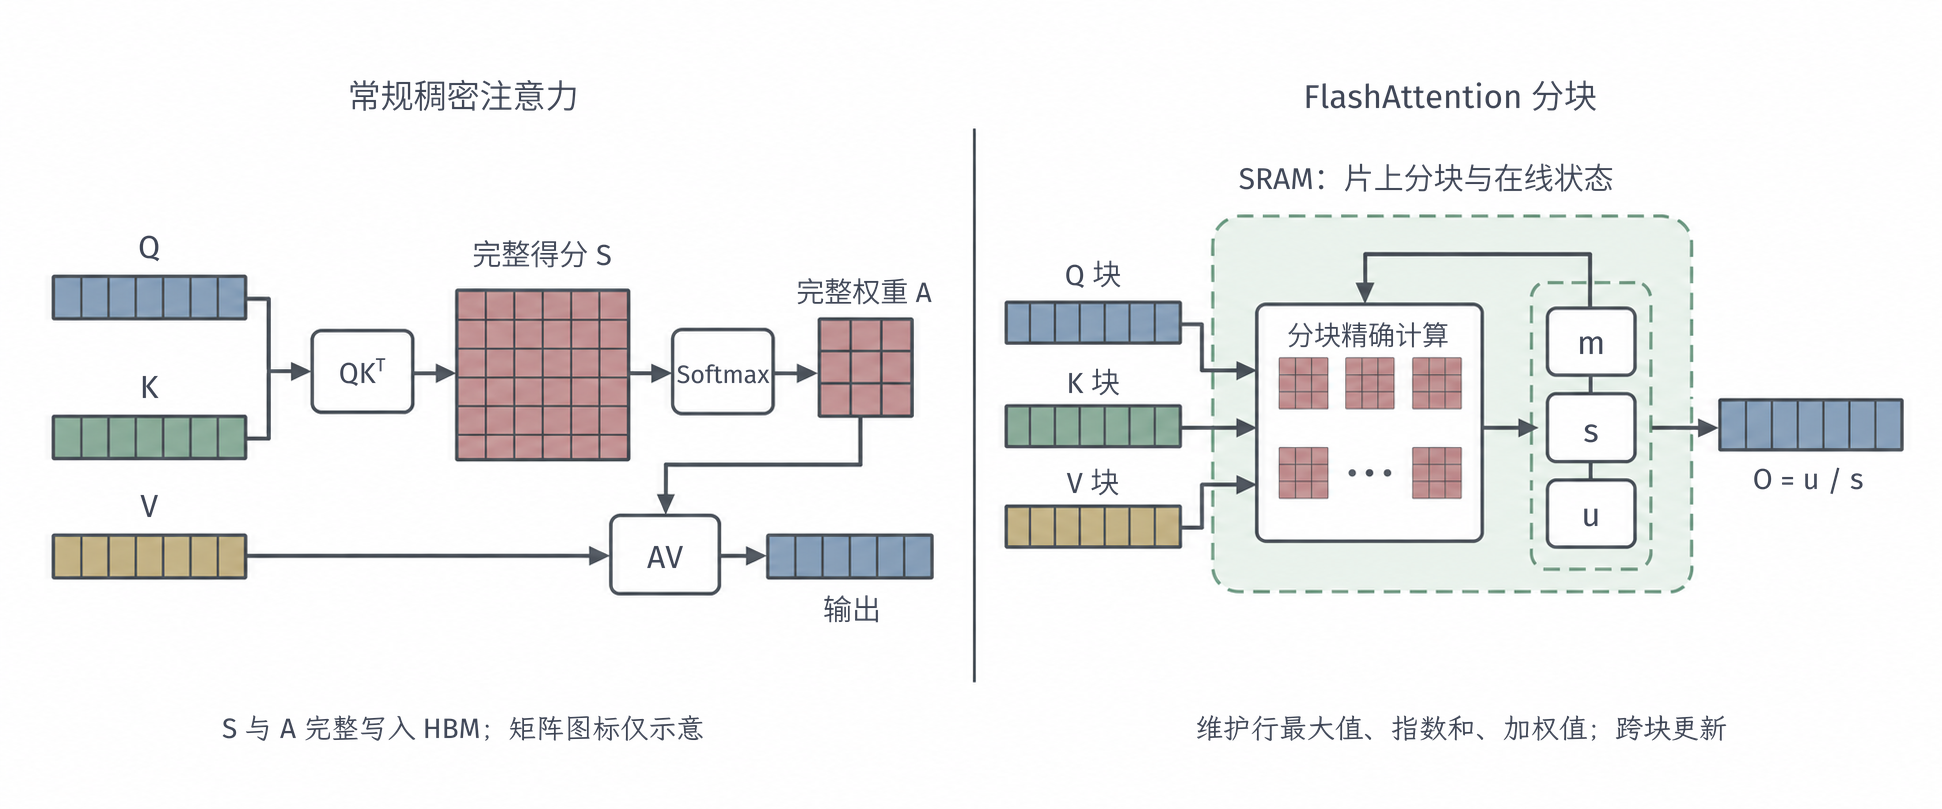
\includegraphics[width=164.423mm]{figures/05-neural-network-models/00-shared/generated/transformer-flashattention/figure.png}
  \caption{FlashAttention保留稠密注意力结果，改变中间结果的存储与合并方式。左图的常规实现把完整$\bm S,\bm A$写回容量较大的HBM；右图按块在HBM与容量较小的片上SRAM间搬运，只在片上保存当前块和在线统计$m,s,\bm u$。在线合并的分母覆盖全部键，输出与同一稠密注意力计算一致。图为存储与计算路径示意，教学数值在正文展开，反向重算细节省略。}
  \label{fig:transformer-flashattention}
\end{figure*}



\subsubsection{推理效率：历史缓存与请求分配}

增量生成需要反复读取历史键值，还要为不同长度请求分配存储。以下方法分别改变缓存内容与存储组织。

\paragraph{减少KV缓存容量与读取带宽：MQA与GQA}

解码时，标准MHA为每头保存一套键和值。在服务大模型时，这批KV缓存往往比模型本身还吃显存，因为模型参数只有一份、KV缓存却要按“并发请求数$\times$序列长度”成倍增长，而每个头的键值内容其实高度相似。一个自然的省法是让多个查询头共享同一组键和值：查询仍各自独立评分，但被查询的键值表不再每头存一份。\term{多查询注意力}（multi-query attention, MQA）保留多个查询头，让它们共享一组键值；\term{分组查询注意力}（grouped-query attention, GQA）将$h$个查询头分组，共享$g$组键值，其中$1\leq g\leq h$，是“每头一套”与“全体共享一套”之间的折中。设映射$\rho(a)$把查询头$a$分到键值组，则该头读取$\bm K_{\rho(a)},\bm V_{\rho(a)}$，仍有自己的一行Softmax和输出。

当$d_k=d_v$时，缓存元素数由$2Lnhd_k$变为$2Lngd_k$；MQA对应$g=1$，MHA对应$g=h$。例如$L=24$、$n=4096$、$h=16$、$d_k=64$、每元素2字节的单序列MHA缓存约为384 MiB，$g=4$的GQA约为96 MiB，MQA约为24 MiB。这组教学容量由键值元素数计算；权重、其他激活及分配管理另占存储。

\begin{figure*}[htbp]
  \centering
  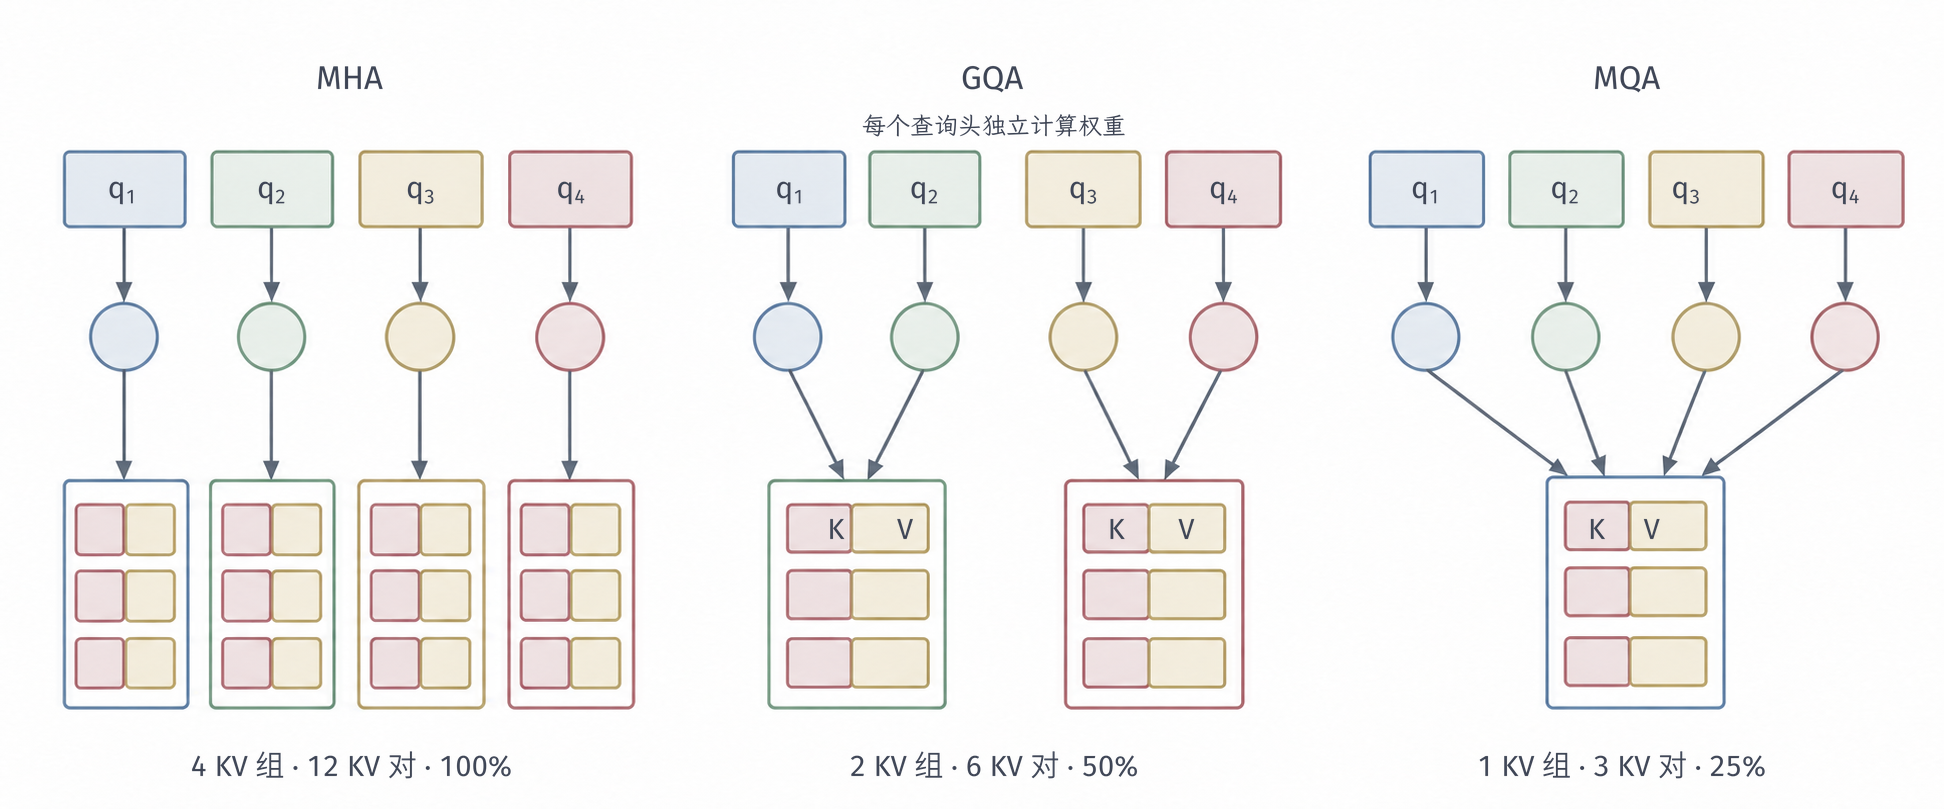
\includegraphics[width=164.592mm]{figures/05-neural-network-models/00-shared/generated/transformer-kv-sharing/figure.png}
  \caption{相同历史序列在MHA、GQA和MQA中的缓存布局。每个缓存小格代表一个历史位置在一组投影下的一对键和值；大框是一整组历史缓存，查询头的箭头指向所读取的缓存。4个查询头分别使用4组、2组或1组键值时，缓存为12、6或3对，下方标出的缓存容量相对于MHA依次为$100\%$、$50\%$和$25\%$。共享发生在键值表示及其存储上，各查询头仍独立计算注意力权重。图只计一层的一条序列，不含当前新位置追加的缓存。}
  \label{fig:transformer-kv-sharing}
\end{figure*}

图~\ref{fig:transformer-kv-sharing}固定3个历史位置“猫、追、狗”和4个新查询头，逐项数缓存中的键值对。MHA为每头保留3对，共12对；两组GQA保留6对；MQA只保留3对。MHA中同一历史位置对应4个缓存小格，表示该位置经过4组不同投影后产生的4对键值，四组投影分别产生自己的数值。共享后，不同查询仍分别与所读键匹配，所以可能得到不同的概率和输出。



Shazeer提出MQA以减少增量解码的键值访存，Ainslie等用GQA提供共享程度与质量之间的中间选择。共享减少了键值投影和缓存自由度，但查询头仍需分别匹配；查询仍逐头评分，评分算术量与缓存容量的$g/h$比例因此按不同操作统计。缓存读取若能在实现中复用，带宽需求才会相应改善，质量和速度都需要在给定模型与硬件上评价\scite{shazeer2019mqa} GQA还可由已有多头模型进行参数转换并继续训练，键值参数合并会改变表示，后续训练用于适应新的共享结构\scite{ainslie2023gqa}

\paragraph{提高KV缓存内存利用率：PagedAttention}

缓存容量之外，还存在分配问题，而且它是典型的“操作系统式”浪费而非容量问题：不同请求的长度持续增长，若像连续数组那样为每个请求预留一整段最大长度空间，请求较短时空闲区域无法分给别人，产生外部碎片；更常见的是，成百上千个请求往往共享同一段系统提示前缀，这份前缀的键值却被各自完整复制了许多遍。借鉴虚拟内存按页管理的思路，\term{分页注意力}（PagedAttention）把缓存划分为固定容量块，用块表把序列的逻辑位置映射到实际存储位置；序列增长时追加块，而不要求整段缓存连续。共同前缀可以引用同一批块，分叉后按需要复制，避免直接修改仍被其他请求读取的数据\scite{kwon2023pagedattention}

若每块容纳$b$个位置，长度$n$需要$\lceil n/b\rceil$块，最后一块的内部空余少于$b$个位置，另有块表和管理开销。原来连续存储中的外部碎片和重复前缀可由此减少，实际键值按所保存的位置继续占据空间，节省的是预留空闲、碎片和重复前缀。PagedAttention改变缓存寻址和共享，MQA/GQA改变键值组数，FlashAttention改变注意力中间结果的执行方式；三者处理不同问题，可在兼容实现中组合。块调度、并发服务和硬件算子的细节由系统卷展开。

图~\ref{fig:transformer-pagedattention}用两个请求演示块表的作用。为便于说明，把“请／解释／注意力／机制”和“请／解释／位置／编码”各视为4个词元，每块放2个位置。本图的词元位置与逻辑块均从0编号。A按物理块$3\rightarrow1$读取，B按$3\rightarrow4$读取，两者共享前缀块3，物理块2仍可供其他请求使用。读取A中位置$i=1$的“解释”时，逻辑块为$\lfloor1/2\rfloor=0$，块内偏移为1；查A块表索引0得到物理块3，再从其中的偏移1取出键和值。词元位置给出逻辑顺序，块表给出物理地址；物理块移动时保持块表对应，位置编码继续使用原逻辑编号。

\begin{figure*}[htbp]
  \centering
  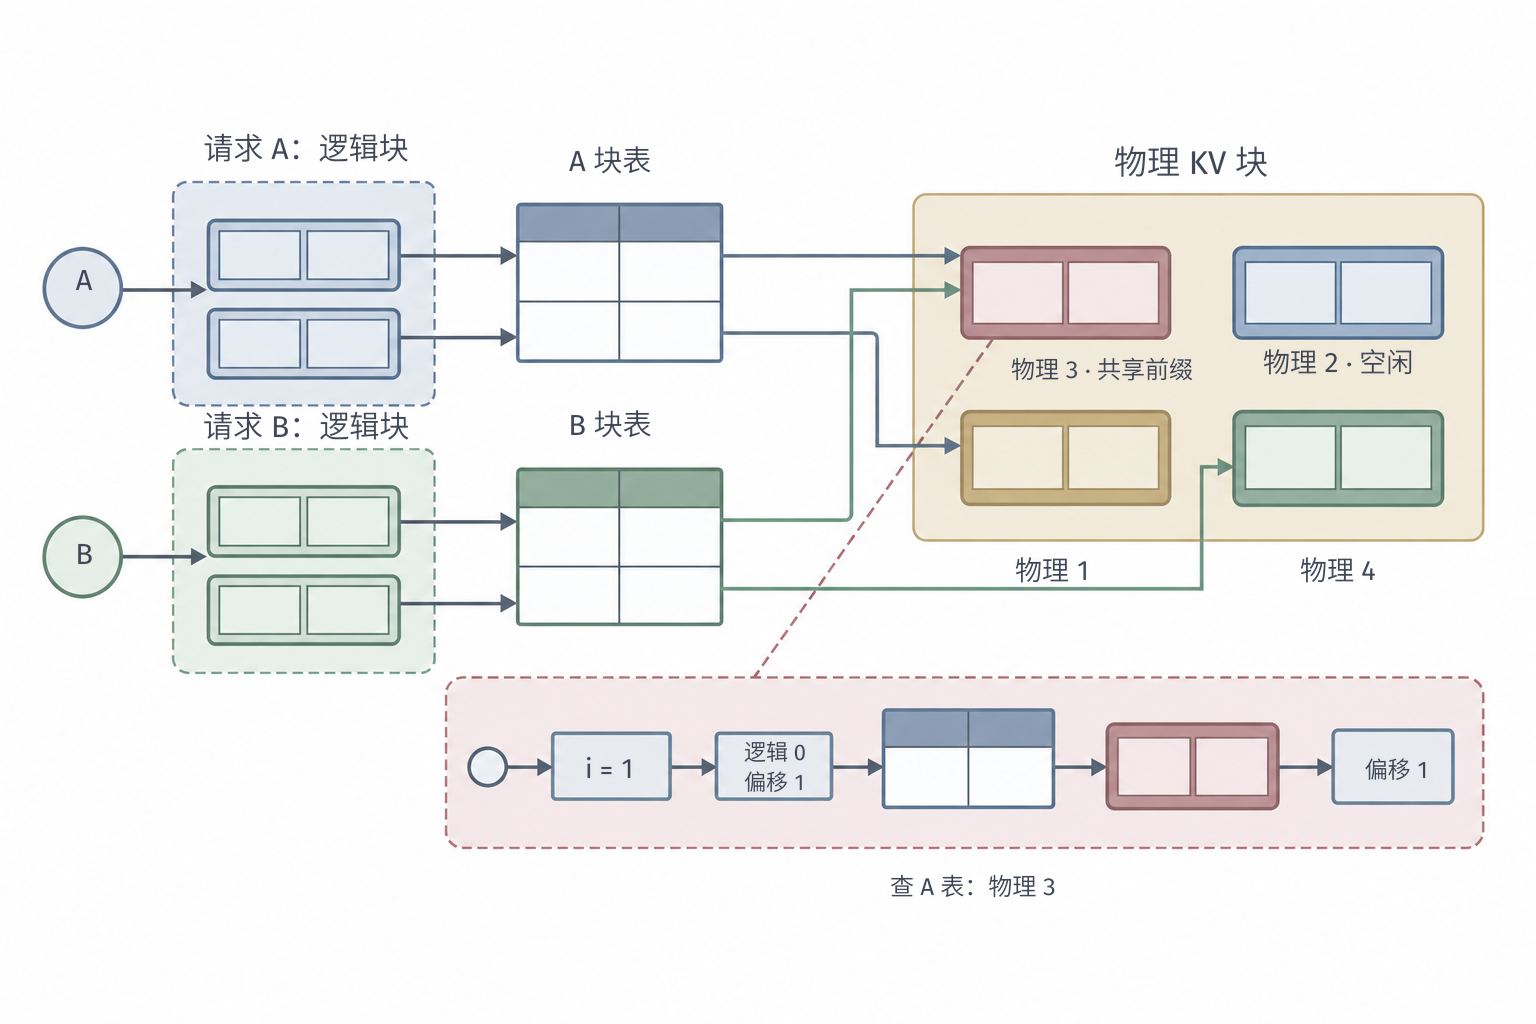
\includegraphics[width=130.048mm]{figures/05-neural-network-models/00-shared/generated/transformer-pagedattention/figure.png}
  \caption{分页键值缓存的具体寻址。上方两条请求按逻辑顺序分块，并用块表保存物理块编号；右侧为实际缓存布局。共享的物理块3只保存一份，A、B的后续各占一块，无需保持物理连续。底部展开一次“位置$\rightarrow$逻辑块$\rightarrow$物理块及偏移”的查找。词元位置、逻辑块和表索引从0开始；物理块编号用1至4标识。缓存小格表示对应的KV内容，正文中的词元例子用于解释寻址，并非把原始文本当作键值向量。}
  \label{fig:transformer-pagedattention}
\end{figure*}

\paragraph{不同扩展方向的比较}

表~\ref{tab:transformer-attention-extensions}把模型变化与实现变化分开。长序列算术量由实际位置连接与聚合决定，FlashAttention改善中间访存，分页改善键值分配。训练概率矩阵与解码历史缓存也有不同生命期，缩小其中一种只节省相应存储。门控、GQA、FlashAttention和分页可以在兼容实现中组合，因为它们分别作用于特征选择、键值组织、块内计算和缓存寻址。

\begin{table*}[htbp]
  \centering
  \small
  \begin{tabular}{@{}p{30mm}p{37mm}p{39mm}p{49mm}@{}}
    \toprule
    方法 & 主要改善对象 & 改变标准稠密读取？ & 代价或限制 \\
    \midrule
    前缀等掩码 & 可用信息与任务约束 & 改变允许连接 & 需防止目标或跨段泄漏 \\
    门控注意力 & 输入相关的特征选择 & 增加乘性调制 & 增加参数；不自动减少连接 \\
    稀疏注意力 & 位置对算术量 & 删除部分连接 & 范围受限；依赖连接模式 \\
    线性注意力 & 聚合算术量及历史状态 & 改变核或近似Softmax & 依赖特征维$r$与核表达能力 \\
    低秩注意力 & 交互维度与算术量 & 压缩键值位置 & 近似误差；因果性需另设计 \\
    FlashAttention & 中间存储与显存访存 & 保持公式，舍入可能不同 & 稠密算术仍为平方量级 \\
    MQA/GQA & KV容量与解码带宽 & 跨头共享键值参数 & 改变自由度；评分仍按查询头 \\
    PagedAttention & 缓存分配与前缀共享 & 保持逻辑读取规则 & 块表管理；真实键值仍占空间 \\
    \bottomrule
  \end{tabular}
  \caption{注意力扩展的主要目标与取舍。比较以相同有效输入、隐藏宽度与预测条件为前提；具体算术和存储量见各方法正文。降低算术量、减少访存、缩小KV缓存和减少内存碎片是不同指标，实际速度还取决于实现与硬件。}
  \label{tab:transformer-attention-extensions}
\end{table*}

\subsection{前馈层的扩展}
\label{sec:transformer-ffn-extensions}

同一位置的特征可以通过乘法分支调制，也可以交给少量被选中的前馈网络。门控改变特征变换形式，混合专家改变本次执行的网络分支；二者可以组合，跨位置读取仍由注意力等模块承担。

\subsubsection{门控前馈层：调制特征}

普通FFN先扩张特征，再用统一激活筛选。它有一个特点：某个中间特征是否通过、通过多少，完全由该特征自身的数值经固定激活函数决定，网络无法依据当前整行表示“主动地”决定放行还是关闭某类特征。在LSTM里我们已经见过更灵活的做法——用一个由输入算出的门去逐坐标控制信息通过。把这种乘法门控搬进前馈层，就能让“候选特征是什么”和“这批特征这次该放过多大比例”都成为输入相关的、可学习的决定：设置两条投影分支。\term{门控线性单元}（gated linear unit, GLU）用Sigmoid分支逐坐标调制另一分支；应用于Transformer前馈层的一般形式为
\begin{equation}
  \begin{aligned}
    \bm B&=\bm H\bm W_b+\bm1\bm b_b^{\top},\qquad
    \bm D=\bm H\bm W_g+\bm1\bm b_g^{\top},\\
    \operatorname{GFFN}(\bm H)&=(\bm B\odot\psi(\bm D))\bm W_o
                          +\bm1\bm b_o^{\top}\text{。}
  \end{aligned}
  \label{eq:transformer-gated-ffn}
\end{equation}
两条输入投影均从$d$到$d_g$，输出投影从$d_g$恢复$d$。GLU取$\psi=\sigma$，\term{GEGLU}取GELU，\term{SwiGLU}取SiLU，后两者分别由平滑激活产生乘性调制量。GELU或SiLU可以输出负值且不限定在$[0,1]$，这里的“门控”据乘法作用命名；LSTM的Sigmoid门另外受0至1的比例范围约束\scite{shazeer2020glu}

忽略偏置时，普通FFN约有$2dd_f$个参数，门控FFN约有$3dd_g$个参数。若保持这一参数预算，可取$d_g\approx2d_f/3$；比较同样中间宽度会同时改变参数和计算量。两投影分支提供新的特征组合，同时带来乘法尺度与参数配置的选择。泛化表现需结合相同预算下的任务与训练比较。

图~\ref{fig:transformer-gated-ffn}把“追”这一行的两条分支展开：候选特征$(2,-4)$与调制量$(0.5,2)$相乘，得到$(1,-8)$，再经输出投影恢复$d$维。第二维被放大，说明GEGLU、SwiGLU中的调制量不只是保留比例。这里用二维数值演示乘法，实际中间宽度由$d_g$决定；各位置仍独立处理，没有新增跨位置读取。

\begin{figure}[htbp]
  \centering
  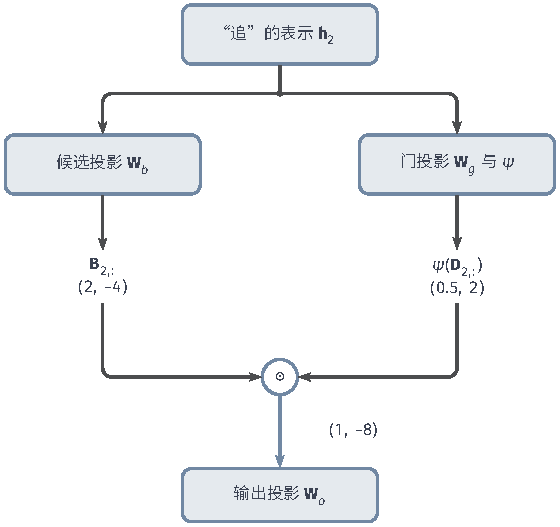
\includegraphics[width=94.791mm]{figures/05-neural-network-models/00-shared/tikz/transformer-gated-ffn/figure.pdf}
  \caption{门控前馈层对“追”的一次逐位置计算。候选特征$(2,-4)$与激活后的调制量$(0.5,2)$相乘为$(1,-8)$，再经输出投影恢复隐藏宽度。数值是教学假设；大于1的调制量适用于GEGLU或SwiGLU的解释，GLU的Sigmoid门则限制在0与1之间。猫、追、狗使用同一套参数分别计算，不发生跨位置读取。}
  \label{fig:transformer-gated-ffn}
\end{figure}

\FloatBarrier
\subsubsection{混合专家：前馈层的条件计算}
\label{sec:transformer-moe-extensions}

逐位置计算还可以按输入选择不同前馈网络。这里针对的是扩大模型时的一个矛盾：想让模型拥有更多可学习参数（更大的知识容量），可若每个位置都要把所有参数算一遍，计算量也随容量同步暴涨，划不来。\term{混合专家}（mixture of experts, MoE）的思路是把容量和单次计算量解耦：准备许多个专家网络，但每个位置只激活其中少数几个，于是总参数可以很多，单位置的实际计算却不随之增长。它设置多个专家和一个路由器，让不同位置使用不同专家组合。\term{专家}（expert）是可训练的特征变换网络，\term{路由器}（router）根据位置表示分配专家权重。设共有$e$个专家，单位置为$\bm h$，路由概率为$\bm p=\operatorname{softmax}(\bm W_{\mathrm r}^{\top}\bm h)$，$\bm W_{\mathrm r}\in\mathbb R^{d\times e}$。若只保留分数最大的$k$个专家集合$T_k(\bm h)$，可以计算
\begin{equation}
  \operatorname{MoE}(\bm h)
    =\sum_{a\in T_k(\bm h)}\widetilde p_a\,F_a(\bm h)\text{，}
  \label{eq:transformer-moe}
\end{equation}
其中$\widetilde p_a$可取选中概率重新归一化后的权重，也可按具体方法保留原概率；训练性质依赖这一约定。总专家参数随$e$增长，一次位置计算主要激活$k$个专家，加上路由器及共享模块的开销，模型存储计入全部专家，本次执行量按被选专家及公共部分分别统计\scite{shazeer2017}

路由可能把大量位置分给少数专家，造成容量不足或计算负载不均。容量限制决定多余位置如何处理，负载均衡辅助目标约束专家使用分布；它们会改变训练目标或输出过程。Top-$k$选择是离散的，常规反向传播只能在当前选择内对连续权重和专家求导，跨越选择边界的行为需要单独设计。若$k=1$并将唯一概率重新归一化为1，仅从这条乘权路径无法训练路由器，尤其需要保留可学习权重或其他训练信号。专家接到哪些输入、形成何种变换，由路由和监督共同学习。设备间派发与汇总还产生通信及调度成本，需在实际执行中另计。

图~\ref{fig:transformer-moe}把路由决策与专家计算分开。对“追”的同一个隐藏表示，假设路由概率为$(0.1,0.6,0.1,0.2)$。Top-2选择专家2和4，再除以所选概率之和$0.8$，得到权重$0.75$和$0.25$。两个专家都读取原隐藏表示$\bm h$，而不是读取路由概率；假设它们分别输出$(2,0)^{\top}$和$(0,4)^{\top}$，加权相加后才得到$(1.5,1)^{\top}$。专家1、3在本次没有执行，参数仍属于模型。这组概率与输出为手算构造，用来对应选择、执行和加权三个环节。

专家通常替换部分块中的FFN，注意力与残差仍可共享。不同位置可以选择不同专家，也可能选择相同专家；路由均衡控制位置怎样分派，输出比例继续由当前路由权重决定。

\begin{figure*}[htbp]
  \centering
  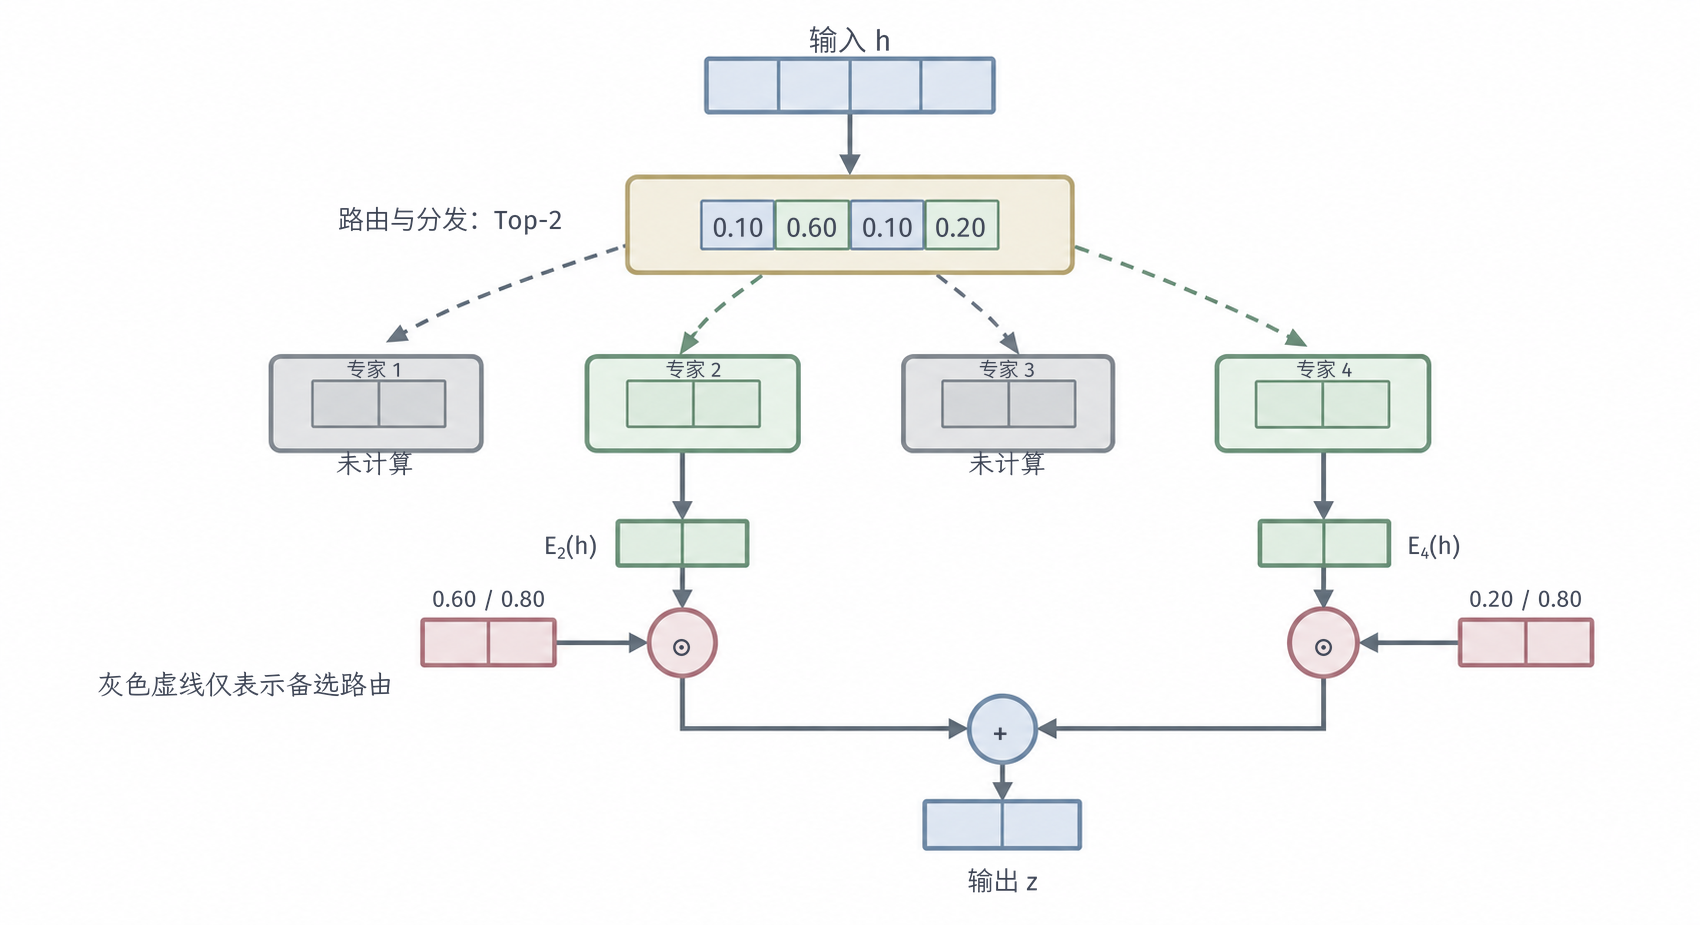
\includegraphics[width=143.933mm]{figures/05-neural-network-models/00-shared/generated/transformer-moe/figure.png}
  \caption{Top-2混合专家的一次完整计算，概率与二维专家输出均为教学设定。上方路由器选出专家2、4并给出重新归一化的权重；下方实线传递隐藏表示、专家结果及乘法所需的标量权重，路由器向各候选专家的虚线表示候选选择关系。专家输入始终是同一个$\bm h$，加权发生在专家输出之后，最终$0.75(2,0)^{\top}+0.25(0,4)^{\top}=(1.5,1)^{\top}$。灰色专家1、3本次不计算；图省略容量限制、辅助训练目标及块外残差。}
  \label{fig:transformer-moe}
\end{figure*}

\subsection{归一化的扩展}
\label{sec:transformer-normalization-extensions}

第\ref{sec:transformer-residual-normalization}节已经给出逐位置LayerNorm及其残差块形式。围绕归一化的种种变体，其实都在回答三个具体问题：沿哪些坐标求统计量、要不要减去均值、以及把归一化放在残差路径的哪一段。选择不同，被消去的信息就不同，信号与梯度通过深层网络的方式也不同。通用归一化公式、批归一化（BatchNorm）、实例归一化（InstanceNorm）和组归一化（GroupNorm）的完整说明见第\ref{sec:training-normalization}节，统计轴对照见表~\ref{tab:training-normalization-axes}。这里集中讨论Transformer中的因果限制、RMSNorm与残差位置。

\subsubsection{统计范围与因果限制}

对批量激活$\bm X\in\mathbb R^{b\times n\times d}$，三个轴分别是样本、位置和特征。式\eqref{eq:transformer-layernorm}固定样本和位置，只沿$d$个特征统计；不同位置不交换均值与方差，训练与预测均使用当前行的统计量，不需要运行均值。在这种逐位置用法中，每份统计都只由当前样本的一行特征形成。

完整已知的图像或离线编码可以使用跨空间、跨位置统计；因果解码则要求位置$i$的统计量不能包含$j>i$的激活。只要均值或方差读取了未来，即使注意力有三角掩码也会泄漏。若BatchNorm、InstanceNorm或GroupNorm采用跨整段统计，因果解码需要把统计范围限制到当时可用的激活，并使训练与预测采用对应方案。训练用全段统计、预测用前缀统计还会引入额外不一致；填充也不能作为有效观测参与统计。

\subsubsection{不减均值的RMSNorm}

中心化不是调整尺度的唯一方式。在极大模型中，LayerNorm里“求均值再逐坐标减去均值”这一步也要消耗可观的计算，而且对很多任务而言，真正需要控制的主要是向量整体幅度（决定点积大小），至于均值是否为零并不关键。\term{均方根归一化}（root mean square normalization, RMSNorm）因此做减法：不减去均值，只按坐标均方根缩放，省下中心化的开销：
\begin{equation}
  \operatorname{RMSNorm}(\bm x)
    =\bm\gamma\odot\frac{\bm x}
       {\sqrt{d^{-1}\sum_{k=1}^d x_k^2+\varepsilon}}\text{。}
  \label{eq:transformer-rmsnorm}
\end{equation}
这里采用常见的无平移形式。它与逐位置LayerNorm均只读取当前行，但少了均值计算和相减。给各坐标加同一常数时，LayerNorm的中心化结果不变，RMSNorm的结果一般会变；忽略$\varepsilon$时，二者都消去正比例整体缩放，实际耗时仍由实现与形状决定\scite{zhang2019rmsnorm}

逐位置统计只读当前行，同时可能消去行内均值或整体幅度。任务需要这些量时，应保留相应信息路径或调整统计方式。只调整整行长度的尺度归一化（ScaleNorm）见第\ref{sec:training-scalenorm}节；直接重参数化权重、而非统计激活的权重归一化（WeightNorm）见第\ref{sec:training-weightnorm}节。ScaleNorm调整激活长度，WeightNorm调整参数表示，与LayerNorm消除行均值的操作分别比较。

\subsubsection{归一化位置：Pre-LN、Post-LN与组合}

归一化的位置改变残差路径。Post-LN子层$\bm y=\operatorname{LN}(\bm x+F(\bm x))$的Jacobian矩阵为$\bm J_{\mathrm{LN}}(\bm I+\bm J_F)$，直接路径也要经过LN；Pre-LN的Jacobian矩阵为$\bm I+\bm J_F\bm J_{\mathrm{LN}}$，恒等路径绕过LN。Xiong等在特定初始化与模型分析下比较了两者的梯度尺度，并解释了原始Post-LN训练中学习率预热的重要性；论文的比较对应特定初始化与模型，其他深度和优化配置下的梯度及效果还需按实际计算检验\scite{xiong2020layernorm}

也可以在子层前和输出端分别归一化，控制输入与支路输出的尺度。例如，把子层的归一化输入记为$\bm u$，计算
\begin{equation}
  \begin{aligned}
    \bm u&=\operatorname{Norm}_{\mathrm{in}}(\bm x),\\
    \bm y&=\bm x+\operatorname{Norm}_{\mathrm{out}}(F(\bm u))\text{。}
  \end{aligned}
  \label{eq:transformer-combined-normalization}
\end{equation}
它与$\operatorname{Norm}(\bm x+F(\bm x))$不同，归一化这里只作用于新增支路，原输入直接进入相加。RMSNorm可放在前或后，LayerNorm也可采用不同位置；统计公式规定尺度怎样调整，放置位置规定哪条路径接受调整。归一化分母、可学习缩放、残差累积和末端读出共同影响信号，整网梯度需要沿这些模块的组合追踪，稳定条件同时涉及分母、缩放与分支累积。

\subsection{深层连接的扩展}
\label{sec:transformer-deep-connections}

直接堆叠残差块仍可能积累过大的更新或使深层分支难以学习。残差虽然给了恒等路径，但每个子层都无条件地把自己的增量全部加进去；层数很多时，这些增量叠加仍可能让表示尺度失控，而且在训练最初、各子层还很“生涩”时，让它们全力改变表示未必有利。一个自然的想法是给每个新增分支再配一个可调节的闸门，让网络自己决定这一层该往原表示里掺入多少新东西。一般子层可写为$\bm h^{(l)}=b_l\bm h^{(l-1)}+a_lF_l(\bm h^{(l-1)})$，其中$a_l$控制新增变换，$b_l$控制原表示的传递。固定缩放可以与深度相关，可学习缩放则让训练决定每条分支的影响；它们都要与归一化和初始化共同考虑。

\term{ReZero}给每条残差支路设置一个初始化为0的可学习标量$a_l$，使用$\bm h^{(l)}=\bm h^{(l-1)}+a_lF_l(\bm h^{(l-1)})$。在该残差堆叠不含其他破坏恒等路径的操作时，初始映射和局部Jacobian矩阵都是恒等。初始步骤中支路内部参数梯度受$a_l=0$抑制，但门参数有梯度$\partial\ell/\partial a_l=\langle\bm g^{(l)},F_l(\bm h^{(l-1)})\rangle$，门偏离0后支路开始收到监督。门参数首先决定支路参与的强度，内部参数可以从非零初始化开始\scite{bachlechner2020rezero}

门也可以是逐特征向量或输入相关函数，形成不同粒度的残差控制。向量门增加参数，自适应门增加计算和新的梯度路径；Sigmoid门如果希望初始接近关闭，偏置与饱和程度就需配合。更广的跨层连接还可把早期层的表示相加或拼接到深层，相加要求维度匹配，拼接会增加宽度并通常需要投影。这些改变影响表示复用、保存激活的数量和梯度路径，整网求导汇合所有分支，优化行为由实际复用和完整梯度共同决定。

图~\ref{fig:transformer-residual-extensions}对照归一化位置与支路缩放。把Norm移到子层之前，保留的是绕过Norm的恒等路径；在支路加入标量，控制的是新增变换的强度。这两个选择可以同时使用。

\begin{figure}[t]
  \centering
  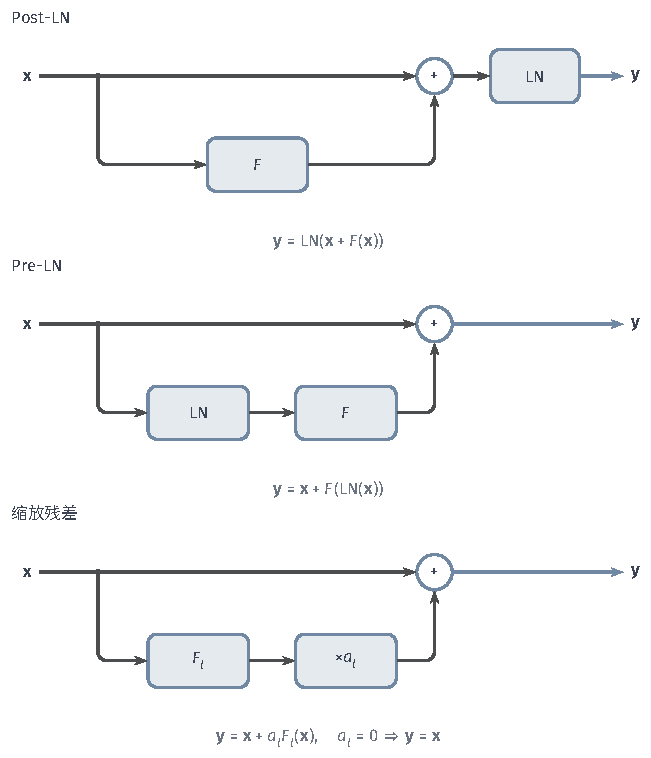
\includegraphics[width=110.225mm]{figures/05-neural-network-models/00-shared/tikz/transformer-residual-extensions/figure.pdf}
  \caption{把恒等路径放在同一水平线上比较三种残差组织。Post-LN的原输入在相加后仍通过LN；Pre-LN只有下方变换支路经过LN，恒等路径可以直接到达输出。第三行以$a_l$缩放新增变换，$a_l=0$时该子层输出等于输入；ReZero采用这一初值，图中省略可选归一化。各行上方路径传递原表示，下方路径计算新增变换，$+$为逐元素相加。}
  \label{fig:transformer-residual-extensions}
\end{figure}

\subsection{混合网络结构}
\label{sec:transformer-hybrid}

稠密注意力保存位置表示并显式读取它们，功能强大但代价是平方复杂度；卷积、循环、状态空间等模块则各有所长——它们擅长低成本地处理局部模式或用固定大小状态压缩历史，却不具备注意力那种“按内容任意直连”的能力。一个自然的工程问题是：能否让不同模块各管自己擅长的一段，而不是让注意力独自承担全部位置交互？局部窗口与固定容量历史状态可以由其他模块提供，与这份逐位置存储组合。若输入具有稳定局部模式，可以用卷积前端提取特征、降低分辨率，再把特征位置送入Transformer；窗口内部的卷积共享与注意力的内容相关读取承担不同职责。下采样减少序列长度，会明显改变后续平方位置对成本，也可能丢失细粒度信息，输出任务需要保留或恢复相应分辨率。

模块也可以交替堆叠。例如用状态空间模块压缩历史，用注意力层在保留位置之间进行显式检索；或者先用循环网络处理陆续到达的观测，再在给定窗口内交换信息。串联改变后一个模块接收到的表示，前端压缩决定后续可用内容，细节若没有保存在输出或旁路中，注意力就只读取剩下的表示。并行分支则可以分别形成局部与全局表示，再相加或拼接，维度、位置对齐和因果规则仍需一致。

各模块的成本沿实际执行累加：只要保留稠密注意力层，整段处理仍有平方量级的位置对计算；生成时，该层需保存随历史长度线性增长的KV缓存。训练中间存储另取决于实现，FlashAttention不必保存完整的平方规模注意力矩阵；固定状态节省相应模块的历史存储，保留的注意力层仍需自己的键值。前端、交替与并行是不同组织方式，应围绕任务需要的局部模式、精确历史读取、延迟和计算预算选择。

图~\ref{fig:transformer-hybrid}比较前端、交替与并行三种组织。它们分别改变输入粒度、层间分工与融合方式，使用哪一种都需要保持位置对应和信息可见规则。

\begin{figure*}[htbp]
  \centering
  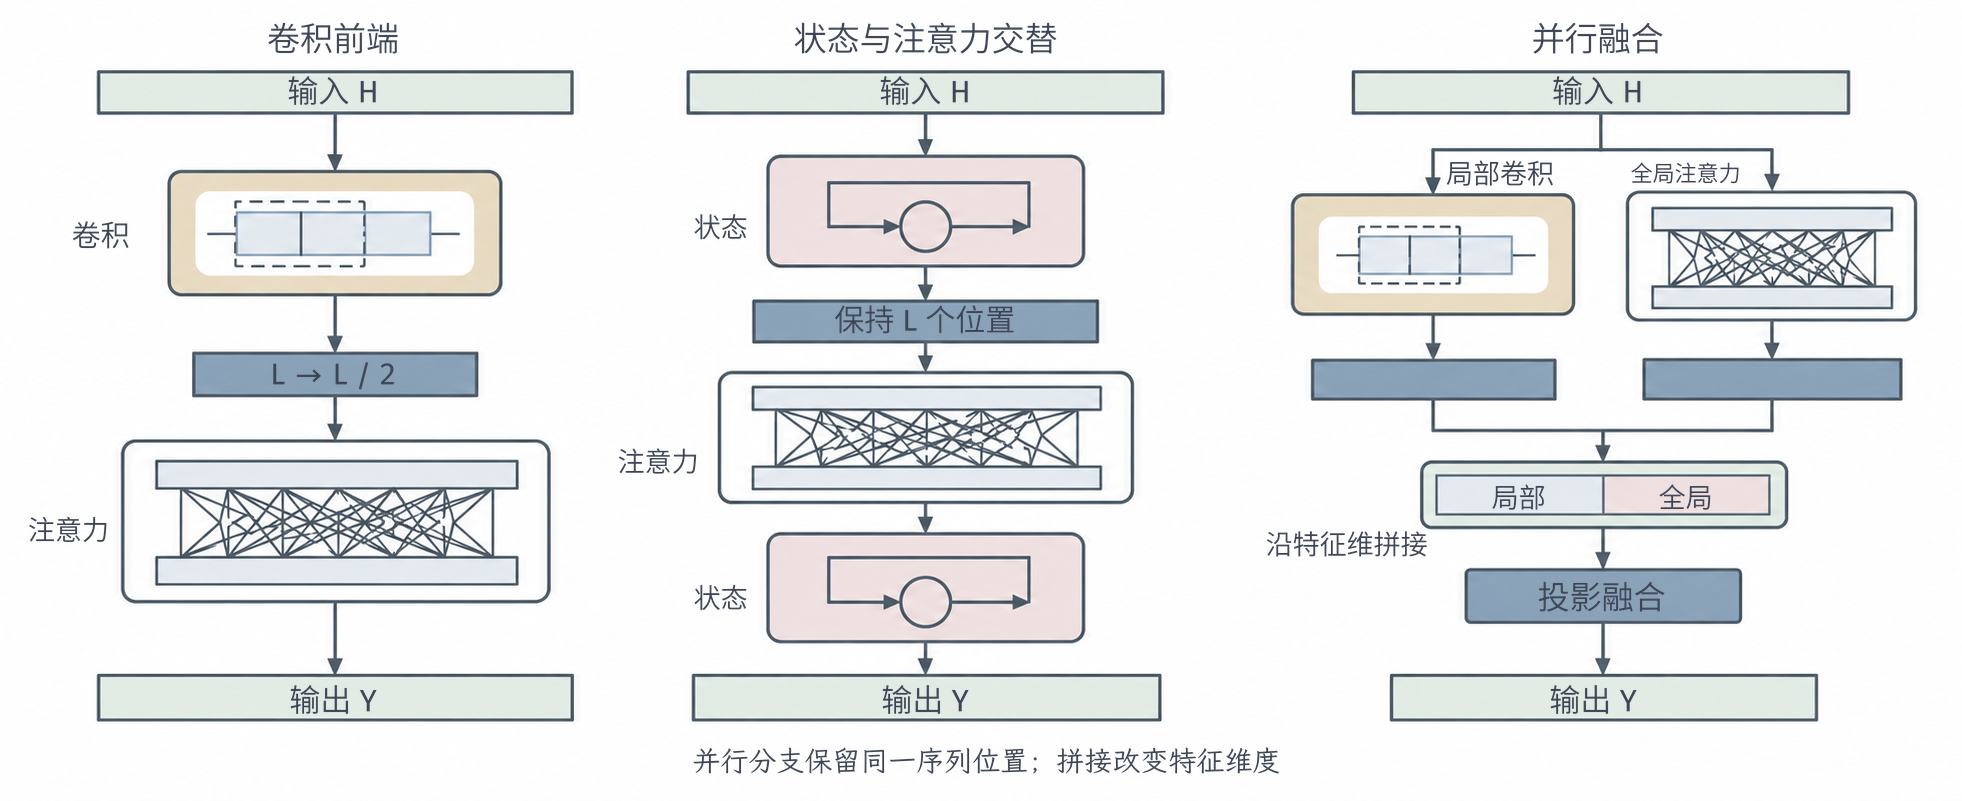
\includegraphics[width=166.116mm]{figures/05-neural-network-models/00-shared/generated/transformer-hybrid/figure.png}
  \caption{三种混合结构改变的是不同环节。左图在$L$为偶数、无填充的设置下，以窗口2、步长2的卷积前端将$L$个输入位置变成$L/2$个特征位置，再交给注意力；中图沿输入位置递推状态，并将各位置输出交给注意力层，随后继续交替；右图对同一序列并行计算局部卷积和注意力，拼接框沿特征维合并两路表示，再经投影融合。并行分支采用保持长度的位置对齐设置，所有分支还需满足任务的因果约束。}
  \label{fig:transformer-hybrid}
\end{figure*}

\FloatBarrier

\section{理论分析}
\label{sec:transformer-theory}

注意力能够跨位置读取，但读取范围、位置信息和数值尺度仍然限制所得表示。这里保留这些结构特有的条件；一般优化与统计推导沿用前面章节。

\subsection{表达能力}
\label{sec:transformer-expressivity}

没有位置或其他顺序线索、并采用对称汇聚的自注意力分类器，对相同词元的排列给出相同结果。因此$(a,b)$与$(b,a)$不能仅靠增加头数或层数得到区分。因果掩码则规定每个位置只能使用前缀，不能完成必须读取尚不可见后文的判断。

在固定长度、可学习位置编码及指定注意力与前馈结构下，Transformer可以逼近相应连续目标；Yun等的结论采用$L^p$积分误差，并允许深度随目标和精度改变\scite{yun2020transformeruniversal}。它不直接保证固定大小、不同掩码或归一化配置的模型具有同样能力，也不提供训练成功或长度外推保证。

\subsection{训练中的数值尺度}
\label{sec:transformer-convergence}

查询和键的尺度共同决定Softmax得分。权重过于集中时，评分路径的梯度可能变小；多头、残差和归一化又影响深层传播，因此需要结合投影尺度、归一化分母和梯度观察选择训练设置。一般光滑目标的优化结论见第\ref{sec:ffn-convergence}节，残差路径的存在本身不保证全局收敛。

硬Top-$k$路由还可能在专家集合切换时产生输出跳变。专家内部可微，不代表整个选择过程光滑；对这类结构，不能直接把连续网络的梯度结论当成路由参数的保证。固定的可见范围、正的归一化分母及实际采用的更新规则，都需要与训练条件对应。

\subsection{泛化性}
\label{sec:transformer-model-generalization}

在独立同分布序列和相应输入、参数及损失约束下，可以沿用复杂度或稳定性结论分析新样本风险，可参考\BookChapterRef{chap:deep-learning-theory}{卷3《基础、理论与可信性》的“深度学习的可学习性”章}。样本数应按实际独立记录计，同一文档的词元或重叠窗口不能各算一份独立证据。预训练、位置编码和缓存扩展了能够处理的输入，不自动保证新领域或更长序列上的误差；这些条件需要用对应数据单独检验。

\FloatBarrier

\section{常见应用}
\label{sec:transformer-applications}

应用中的完整模型需要把输入单位、可见信息、输出含义和监督位置对应起来。同一个Transformer骨架，之所以能用于看起来差异很大的任务，关键不在换了什么神秘结构，而在如何回答前面反复出现的那几个问题：输入切成什么单位、每个位置预测时允许看到谁、输出向量的每一维代表什么、损失加在哪一行。下面三个小节分别对应三种典型的对应方式——整段一个答案的分类、每个位置一个标签的标注，以及逐个产生输出的生成；阅读时可对照6.2节的输出头理解。以下沿用前文的网络块与损失，只展开从样本到预测的路径；数据构建、任务专用结构与评价方法由应用卷细化。

\subsection{文本分类与序列标注}
\label{sec:transformer-text-applications}

评论情感分类的样本是文本和类别。分词后查表形成嵌入，加位置表示，使用双向编码器得到上下文表示，再采用CLS或掩码池化读出，经Softmax分类。以“这部电影并不精彩”为例，编码器给“精彩”的表示可以读取否定上下文，整段分类头据此输出类别。否定关系提供这项任务需要的证据，模型通过哪些头和特征使用它，可以结合响应分析；最终预测由独立样本评价。

训练对评论计算交叉熵，嵌入、编码器和分类头共同更新；如果先使用已有模型，再训练任务头或微调部分层，需要明确哪些参数更新。推理使用同一分词与有效位置规则，输出整段概率。截断删去的文本可能包含判断证据，训练和测试的长度处理因而共同规定实际预测条件。

实体标注则将每个有效位置表示送入共享分类头，计算对应标签损失。若一个词被拆成多个子词，标签需选择监督首个子词、监督所有子词，或先聚合为词表示，推理时也用同一规则。逐位置Softmax分别形成标签概率，跨位置标签组合若有约束，还需由相应输出模型联合处理。离线标注读取整段，流式标注使用因果或有限延迟范围，这个约束比“采用编码器还是解码器”的名称更直接。

\subsection{序列转换与生成}
\label{sec:transformer-generation-applications}

机器翻译训练使用源句$x$和包含EOS的目标$y$。源嵌入和编码器产生$\bm H_{\mathrm s}$，目标输入右移，因果自注意力读取真实目标前缀，交叉注意力读取有效源位置，以式\eqref{eq:transformer-conditional-loss}更新两侧嵌入、所有网络块和词表输出层。源词和目标词通过条件似然共同训练，注意力权重由这份翻译监督学习软对应。

推理时源端只编码一次，各目标层还可预先缓存该层交叉注意力的源键值。目标从BOS开始，每次前向为当前输入计算并追加各层自注意力键值，再由词表头产生下一词元分布。选出的词元作为下一次输入，逐步延长缓存，遇到EOS或长度上限停止。不同层的投影参数不同，因此源交叉键值与目标自注意力键值都按层保存。束搜索存在多个候选前缀时，可以共享未变的缓存内容，分叉后的修改则需各自维护或按写入时复制处理。

文本续写不需要独立源编码器。已给定提示先做预填充，末位置输出预测提示后的第一个词元；把选出的词元作为新输入，在各层追加缓存，得到下一词元分布。续写读取已经产生的完整前缀，训练则读取真实前缀；两种输入来源决定模型实际经历的上下文。选择温度、采样或搜索策略会影响输出，评价需使用实际采用的生成过程。

\subsection{图像分类}
\label{sec:transformer-vision-applications}

图像具有二维网格位置，注意力读取的却是“一串向量”，要把图像交给Transformer，先要解决“怎样把二维图像变成一串位置”。一个朴素想法是把每个像素当一个位置，但像素数量动辄上百万，平方注意力完全无法承受；而且单个像素几乎不含语义，模型真正需要交互的是“一小块一小块”的局部区域。因此折中的做法是把图像切成若干小块，每块经一次投影变成一个向量，块与块之间再做注意力——位置数从像素数降到块数，变得可负担。\term{视觉Transformer}（Vision Transformer, ViT）将图像分成块，分别嵌入后进行位置间注意力，再读出图像类别\scite{dosovitskiy2020vit}

设图像高宽为$H,W$、通道数为$c$，块边长为$p$，并暂设$H,W$可被$p$整除，则块数为$n=HW/p^2$，每块展平向量$\bm x_i\in\mathbb R^{p^2c}$。投影后的输入为
\begin{equation}
  \bm h_i^{(0)}=\bm W_{\mathrm p}^{\top}\bm x_i+\bm b_{\mathrm p}+\bm p_i,
  \qquad \bm W_{\mathrm p}\in\mathbb R^{p^2c\times d}\text{。}
  \label{eq:transformer-vit-input}
\end{equation}
位置索引按固定网格顺序排列，位置表示须保留块与空间位置的对应。加入专用分类位置后，共有$n+1$行表示，经编码器、末端归一化和分类头产生概率，以图像标签交叉熵训练。图~\ref{fig:transformer-vit}把图像块、序列表示与分类输出连接起来。

\begin{figure*}[htbp]
  \centering
  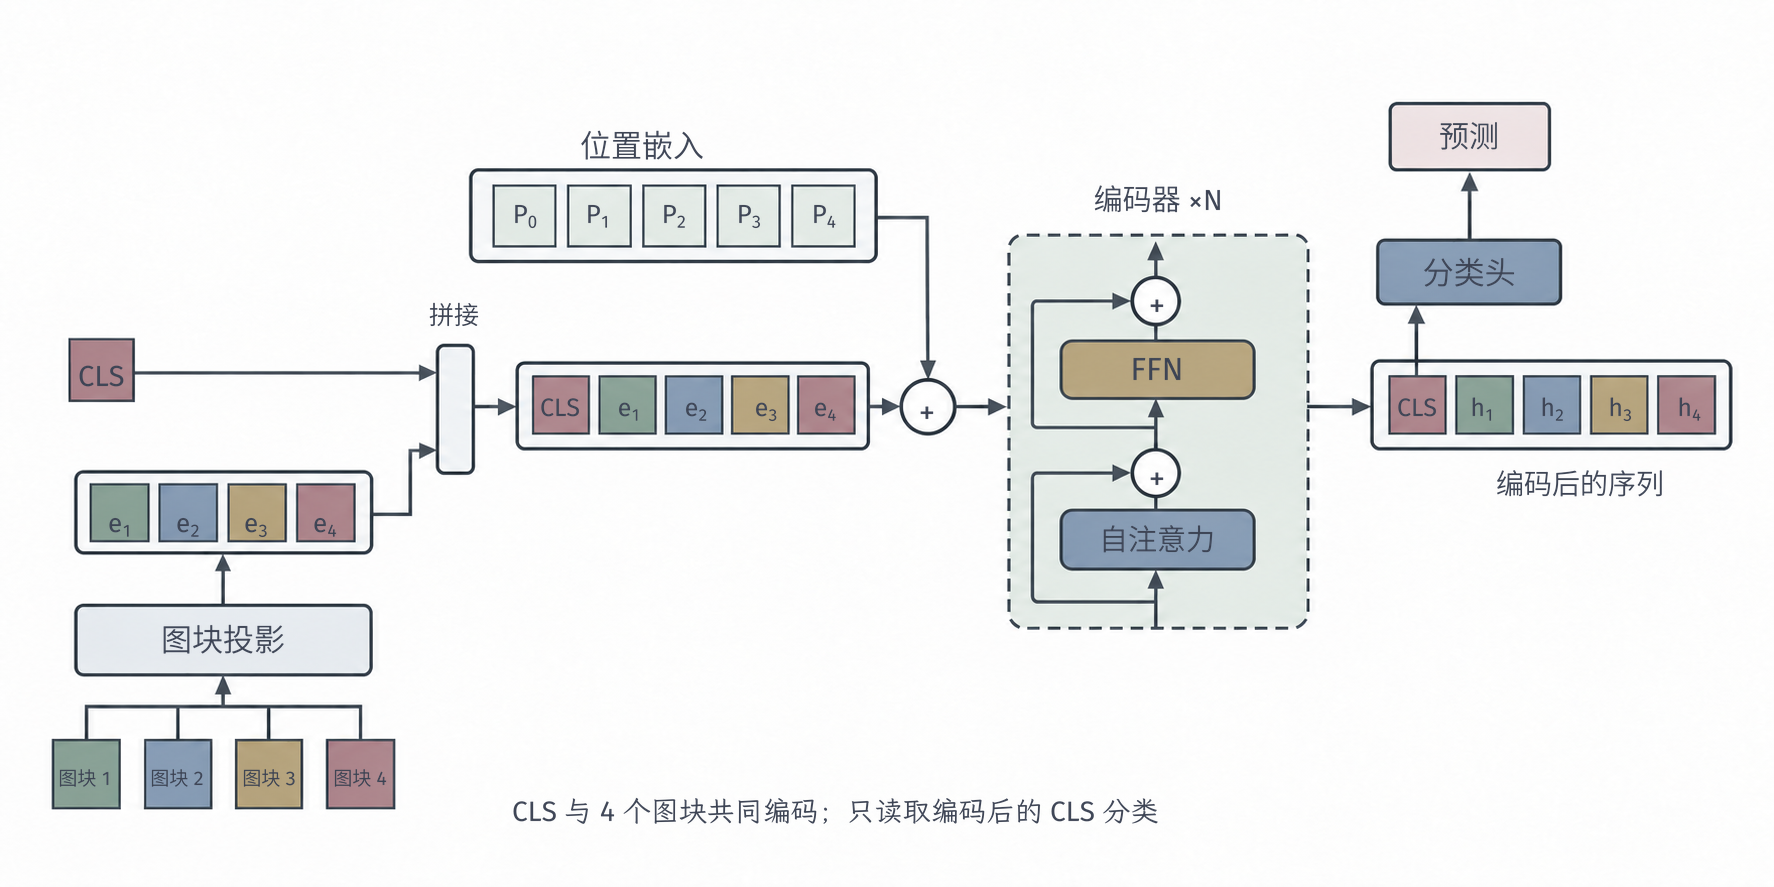
\includegraphics[width=150.199mm]{figures/05-neural-network-models/00-shared/generated/transformer-vit/figure.png}
  \caption{ViT将图像组织为序列的过程。四个示意图像块按固定空间顺序编号；每块展平后通过同一线性投影形成$\bm e_i$。在开头加入可学习CLS表示，为五行分别加入位置向量，再送入双向编码器。分类头只读取末层CLS行，其他图像块通过注意力参与其形成。图像块色块仅为结构示意，不声明实际像素尺寸，也不是识别实验样本。}
  \label{fig:transformer-vit}
\end{figure*}

图像块之间可直接交互，但块内部结构在原始ViT中经一次线性投影进入表示，没有逐层卷积的局部共享假设。较小的$p$保留更细的位置划分，同时使$n$增长；固定图像尺寸时，稠密注意力位置对数与$p^{-4}$同阶，前馈层的块数成本则与$p^{-2}$同阶。改变图像分辨率会改变网格和位置数量，可学习位置表常需按空间网格插值；插值提供新网格的位置向量，分类质量还取决于新增图像细节与已学规则的匹配。数据量、预训练、局部模块和增强会影响实际效果，ViT与卷积模型的实际比较需要固定数据、训练投入和评价目标，局部归纳假设与预训练知识共同影响结果。

\FloatBarrier
\section{本章小结}
\label{sec:transformer-summary}

Transformer把序列中的位置依赖转为显式读取：内容表示给出查询、键和值，位置表示和掩码约束怎样匹配以及哪些位置可见，多头注意力形成不同聚合，逐位置前馈网络再组合这些特征。残差和归一化让这套计算能够层层堆叠。与循环注意力相比，它可以同时更新已知位置。逐步生成时，新的输出依次成为后续条件，缓存保存已完成的位置计算以便复用。

结构与资源的选择需要同时看任务。双向读取适合完整输入理解，因果读取满足在线与生成条件，交叉注意力将源目标表示分开。位置扩展提供不同距离规律，门控和专家改变特征选择；稀疏、线性和低秩路线改变读取结构或公式，FlashAttention保留稠密计算而减少中间访存，MQA/GQA缩小键值组数，PagedAttention改善缓存分配与共享。减少哪一种开销、改变哪一种表示自由度，决定了这些方法的组合与取舍。

损失沿值读取、评分、特征变换及直接残差路径汇集为参数梯度，训练进展与预测风险再据各自条件评价。得分尺度、归一化分母、残差深度和长度共同影响学习，独立样本数、参数约束、数据分布和评价目标共同约束风险结论。由此可以回答章首的问题：直接位置交互使已知输入的计算更易并行，但可靠预测还取决于可见范围是否正确、任务信息是否保留，以及学习结果是否在实际使用条件下得到检验。

\paragraph{扩展阅读}
原始Transformer、BERT与GPT-3论文见第\ref{sec:transformer-common-architectures}节，可结合本章公式核对输入、掩码、归一化与监督位置。

\chapter{脉冲神经网络}
\label{chap:spiking-networks}

先从一种特殊的传感器说起。普通相机每隔固定时间拍下一整帧，无论画面有没有变化都要产生并处理一整张图；事件相机则完全不同，它只在某个像素的亮度发生变化时，才送出一个带时间戳的事件——“第几行第几列、在什么时刻、变亮还是变暗”。面对这样的输入，前几章那种“每隔一段时间吃进一个稠密实数向量”的网络就显得别扭：若等够一帧再处理，会白白浪费事件天然带有的精确到达时刻，把“哪次变化先到、哪次后到”的先后信息抹平；若每收到一个事件就重算整张图，又要对绝大多数根本没变的位置做无用功。于是自然产生一个问题：能不能让网络直接以“到达的事件”为基本输入，在处理事件的同时保住它们的强度、先后顺序和更早以前留下的影响？

这个问题的答案，就是本章要讨论的脉冲神经网络。信号在网络里不再以连续实数的形式传递，而是以一个个离散的“发放事件”传递；一个事件本身极其简单，只说明“某个单元在某个时刻发放了”，信息要靠事件的次数、到达的时刻以及单元内部保存的历史状态来共同承载。

生物神经元恰好就是这样通信的：细胞内部的膜电位连续地积累和消退，但神经元向远处发出的信号却是短促、离散的动作电位。液态状态机也已经用固定的脉冲储备池形成随时间演化的动态、再训练一个读出（见第\ref{chap:neural-network-overview}章与第\ref{chap:recurrent-networks}章）。但如果还想让多层连接都能从任务误差中学习，就必须回答：输入怎样编码成事件、单元内部怎样积累历史、连接怎样传播事件，以及最终误差怎样接回到这些离散事件和连续状态上。输入怎样编码，内部怎样积累，连接怎样传播，决定这种通信能完成什么预测；时间模拟与训练则产生相应成本。

阅读本章时可以始终抓住一对区分：单元对外传出的是离散脉冲（0或1的事件），单元内部保存的却是膜电位这样的连续状态。事件在到达的瞬间改变状态，两次事件之间状态仍按自己的规律继续演化，于是很久以前的输入也能影响此刻的响应。本章先用离散时间把连接输入、状态更新、学习和读出完整地串成一条计算路径，再用它解释“事件稀疏”到底在什么条件下才能真正省下计算；其中的连续时间方程则为这些离散更新提供物理与数学上的来源。

\section{脉冲神经网络概述}
\label{sec:snn-overview}

\subsection{提出动机与核心思想}
\label{sec:snn-motivation}

为什么要放着熟悉的实数激活不用，转而研究这种更“原始”的脉冲通信？动机来自生物现实和工程现实两端。生物细胞的膜电位在细胞内是连续变化的，但它向其他细胞远距离通信时，主要靠的是一个个短暂、形状几乎固定的动作电位（脉冲）；如果只用一个实数激活概括细胞的活动，单次发放发生在什么时刻、两次发放间隔多长、阈值以下还在悄悄积累了多少，这些信息就全被略去了。神经科学要解释细胞如何响应输入，就绕不开这些量；而事件相机这类变化驱动的传感器，又恰好直接提供了带精确时刻的观测。

\term{脉冲神经网络}（spiking neural network, SNN）以离散发放事件在单元之间传递信息，单元内部保存随时间演化的状态。一个脉冲通常只报告某单元在某时刻发放；信号的强度和时序关系由发放次数、发生时刻及发放单元共同承载。接收单元积累这些输入，旧输入逐渐衰减，状态越过阈值时再产生新事件。事件序列承担编码，阈值、复位与状态递推形成处理这些序列的网络。

需要强调的是，“用0和1通信”本身并不自动等于省电或更强大，这类模型真正服务的是两类不同的问题，评价方式也不同。神经科学需要用动态解释细胞的输入响应，以及局部连接怎样形成行为，关心的是模型是否符合生物证据；工程则希望在输入变化稀疏时，按到达事件传递和处理信息，减少持续感知中的操作，关心的是端到端的实际开销。后一收益取决于完整链路：传感器与编码到底产生多少事件，网络实际访问多少连接，设备又以什么方式更新状态。仅仅把通信变量取成0与1，并不能推出这些成本。

对本科阶段的工程任务，可以使用只保留积累、泄漏、阈值和复位四种机制的简化单元，通过任务损失学习连接参数，再用连续值读出形成预测——不必复刻真实神经元的全部离子通道。究竟保留哪些细胞机制，应由研究问题决定：解释发放过程需要相应的生物证据，分类需要任务评价，节省计算则需要检查实际执行的事件与状态更新。

\subsection{从神经元建模到神经形态计算}
\label{sec:snn-early-history}

脉冲网络的发展汇合了神经元动态、时序编码和硬件实现几条路线。它们分别解释事件怎样产生、时间怎样承载信息，以及事件怎样被执行。1907年Lapicque的积分发放思想将输入电流的积累与阈值发放联系起来，是早期简化动态模型的一条路线\scite{gerstner2014}

1952年Hodgkin与Huxley从离子电流出发建立动作电位的定量模型。与积分发放模型相比，它解释波形产生机制，说明神经元模型可以在不同生物细节层次上工作：简化模型便于组织较大网络，细致模型则服务于膜电流和发放机制研究\scite{hodgkin1952membrane}

1990年，Mead系统讨论\term{神经形态电子系统}（neuromorphic electronic systems），即借鉴神经系统组织与动态来设计电子计算系统。它关注的不仅是某个神经元方程，还包括局部连接、并行动态和物理实现；神经形态计算的范围因此比某一种SNN模型更广\scite{mead1990neuromorphic}

1997年，Maass以“第三代神经网络模型”讨论脉冲单元的计算能力，把发放时间明确纳入计算。这一代际划分比较阈值单元、连续激活与脉冲时序能够完成的计算。相应表达结论限定了编码和单元模型；实际任务精度与设备能耗还由训练、数据和执行方式决定\scite{maass1997spiking}

脉冲储备池进一步展示了利用复杂动态而不训练全部循环连接的路线。2002年的液态状态机让输入扰动一个固定循环系统，再训练读出使用其动态状态；第\ref{sec:rnn-lsm}节已给出这种分工。局部可塑性则从突触两端活动出发调整连接，为无需完整反向传播的学习提供另一条路径。储备池把可训练部分放在读出，局部规则把可用信号限制到突触附近；多层监督任务还需要把最终误差分配到更早的事件和连接。

\subsection{深层网络与训练方法的发展}
\label{sec:snn-learning-history}

当目标从解释局部动态转为学习多层分类器，离散阈值成为主要困难。2002年，Bohte等提出SpikeProp，根据发放时刻与目标时刻之间的误差进行反向计算；它对发放时刻求导，所需的模型与发放条件限定了这种时间误差回传的用法\scite{bohte2002spikeprop}

后来的两条路线让深度学习经验更容易进入SNN。一条先训练连续值网络，再校准权重和阈值，使脉冲统计近似原激活；另一条在前向保留离散发放，在反向指定替代导数，直接优化任务损失。第\ref{sec:snn-learning}节会分别说明转换误差和替代梯度的近似性质。2019年的替代梯度综述系统整理了后一条路线，替代规则为不连续发放提供了指定的反向信号，前向阈值仍然保留\scite{neftci2019surrogate}

可训练性改善后，研究开始扩展深度与信息交互方式。2021年的SEW-ResNet研究怎样在脉冲残差路径中保持合适的传播；2022年发布、2023年发表于ICLR的Spikformer则将脉冲形式的查询、键和值用于注意力计算。残差组织层间传播，注意力组织信息读取；其中连续运算、时间步使用和硬件映射方式又分别影响训练与执行成本\scite{fang2021spikingresnet}

Spikformer将两种约定组合起来：事件编码与神经元动态规定单元怎样响应，注意力与层间组织规定怎样读取信息。具体模块需要相应的脉冲实现；静态图像还需编码成多步输入，其事件数由这份编码与网络响应决定\scite{zhou2023spikformer}

\subsection{与连续值神经网络的比较}
\label{sec:snn-ann-comparison}

两类网络都可以有前馈、卷积、循环或注意力连接，所以SNN并不是一种全新的“拓扑”，它与普通网络的区别主要落在单元输出的形式和时间动态上。普通前馈单元一次前向就产生一个实数激活，计算结束后内部不留存东西；脉冲单元则先更新内部状态、再决定这一步是否发放，发放与否都是离散事件。即使没有任何循环边，漏积分发放（leaky integrate-and-fire, LIF）单元也能用膜电位把过去若干步的输入记住，而普通逐帧前馈网络通常没有跨帧状态——这一点和第\ref{sec:rnn-lsm}节的LSM呼应。RNN同样保存跨时间状态；SNN与之相比，特殊之处在于明确的阈值发放、发放后复位和以事件进行通信这三件事。

还要特别澄清一个容易混淆的点：同样是一个值为1的比特，在二值网络里它只是某层的离散输出，在SNN里它表示“某个时间区间内发生了一次发放”，含义与内部状态紧紧相连。脉冲单元这一步输出0，并不等于它什么都没“想”——过去的输入可能正悄悄积累在膜电位里，下一个事件到来时就可能叠加越过阈值而发放。表~\ref{tab:snn-ann-comparison}从通信、状态、时间、求导、训练、成本和读出几个方面系统比较两者。
\begin{table*}[htbp]
  \centering\small
  \begin{tabularx}{\linewidth}{@{}p{25mm}XX@{}}
    \toprule
    比较维度 & 连续值网络 & 脉冲神经网络 \\
    \midrule
    通信变量 & 实数激活或向量 & 发放事件；数量与时刻共同承载信息 \\
    单元内部状态 & 前馈单元通常无跨输入状态；RNN有状态 & 膜电位、突触响应及可选适应状态 \\
    时间关系 & 由递推、位置或时间特征表达 & 由事件时刻、积累、泄漏与延迟表达 \\
    求导困难 & 常见激活可微或分段可微 & 阈值发放不连续，需特别处理 \\
    训练路线 & 任务梯度及其他学习方法 & 局部规则、时间求导、替代梯度或网络转换 \\
    执行成本 & 取决于算子、稀疏性与设备 & 还取决于观察窗口、事件访问和状态更新 \\
    输出形式 & 分类分数、概率或连续量 & 计数、发放时间或连续状态读出 \\
    \bottomrule
  \end{tabularx}
  \caption{以常见人工模型比较两类网络。连续值网络也能使用稀疏计算、动态状态和局部学习；SNN也可能在通用设备上按固定时间步进行稠密计算。预测质量和能耗需要在相同输入、决策条件与设备设置下另作比较。}
  \label{tab:snn-ann-comparison}
\end{table*}
\FloatBarrier

\subsection{应用现状与发展方向}
\label{sec:snn-development}

事件视觉、稀疏声音或触觉感知、持续监测与机器人响应，是SNN值得研究的场景：输入随时间到达，变化可能稀疏，决策又关心响应延迟。2017年Amir等将事件相机、脉冲识别网络与TrueNorth处理器用于实时手势识别，给出了传感器到设备执行的完整研究系统。这项研究把事件输入、网络响应和设备测量接在同一链路中，结果对应其手势任务、设备与测试条件\scite{amir2017gesture}

硬件的发展提供了更灵活的实验平台。Loihi面向事件通信、神经元状态和片上学习；Loihi 2进一步支持可编程神经元动态。Intel于2024年公布并部署到Sandia的Hala Point，以Loihi 2构成大规模神经形态研究系统。这项交付为研究设施提供了较大规模的事件计算平台，应用范围由设施中的具体实验与工作负载界定\scite{intel2024halapoint}

应用前景取决于完整链路。若输入本来是密集静态图像，需要编码并模拟许多时间步，事件数量和等待时间可能抵消部分收益；若输入是稀疏事件流，输出还需在较短窗口内可靠形成，噪声、低发放量和阈值校准就更关键。分类结果衡量预测，操作量或能耗估计描述成本模型，实际设备测量则反映执行链路；共同的输入与决策条件使这些结果能够相互对应。

已有发展显示两条仍在推进的路线：一条扩大模型的可训练深度、注意力组织和任务范围，另一条围绕稀疏传感器与专用设备共同设计编码、动态和执行方式。深层任务模型与完整实验系统已经提供了可研究的计算对象。数据适配、训练成本、状态存储和软件执行决定这些对象怎样进入其他场景；后面的结构、学习与理论分析将把这些条件落到编码和动态上。

\section{网络结构}
\label{sec:snn-coding-dynamics}

脉冲网络由输入编码、带状态的神经元、突触连接和读出四部分组成。可以用一个问题串起它们：一个连续变化的外部世界，怎样变成网络能消费的事件（编码）；事件到达单元后留下什么、积累多久、何时再向外发出新事件（神经元动态）；新事件被送往哪些单元、延迟多久到达（突触连接）；最后怎样从一段时间的发放中读出答案（读出）。连接决定事件送到哪里，神经元动态决定事件到达后留下什么状态、何时产生下一次发放。输入编码规定事件含义，单元内部的计算规定历史保留；把这些单元接起来，才得到前馈或循环的信息路径。

\subsection{频率编码与时间编码}
\label{sec:snn-coding}

假设一个传感器在一段时间内观察到某种强度，比如光强是0.7。连续值网络可以直接把0.7这个数喂进去，脉冲网络却必须先回答一个全新的问题：实数0.7要怎样“翻译”成一串0和1的事件？这就是编码要解决的事。对第$i$个输入通道，记发放时刻为$t_{i,k}$。连续时间的脉冲列可以形式化为
\begin{equation}
  s_i(t)=\sum_k\delta(t-t_{i,k})\text{，}
  \label{eq:snn-spike-train}
\end{equation}
其中$\delta$为Dirac脉冲，其意义通过积分给出：对一个只包含某次发放的时间区间积分，得到1。这个表示省略了动作电位的波形，只记录事件时刻。计算机模拟常将时间分为宽度$\Delta t$的$K$个区间，令$s_i^{(t)}\in\{0,1\}$表示第$t$个区间是否发放；若同一区间允许多次发放，可以改用计数，后续计算也相应处理这份次数。

\term{频率编码}（rate coding）用观察窗口内的脉冲数量表示输入强弱：信号越强，发放越密。这是最直观的方案，因为在一段足够长的时间里数脉冲个数，恰好得到一个与强度成正比的连续量。若窗口长度为$T_{\mathrm{win}}=K\Delta t$，计数与频率为
\begin{equation}
  N_i=\sum_{t=1}^{K}s_i^{(t)},\qquad
  r_i=\frac{N_i}{T_{\mathrm{win}}}\text{。}
  \label{eq:snn-rate-code}
\end{equation}
因此，同样的脉冲数即使排列不同，也具有相同的窗口频率。将非负输入$x_i\in[0,1]$编码为每个区间独立以概率$x_i$发放，是一种教学上容易分析的随机方案。它满足$\mathbb E[N_i/K]=x_i$，方差为$x_i(1-x_i)/K$。延长窗口可以降低这种抽样误差，但增加等待时间和期望事件数。这里的方差来自独立抽样；相关发放的计数误差还会包含事件之间的协方差。

如果任务要区分“哪个信号先到”，仅统计数量就从根本上无能为力了——频率编码把脉冲在时间轴上打乱，只留下总数。很多实时任务关心的恰恰是先后：声音先到左耳还是右耳决定了声源方向，前方障碍先触发哪个传感器决定了运动趋势。于是需要另一种编码，让时间本身携带信息。\term{时间编码}（temporal coding）用发放时刻或相对时间关系承载信息。例如，\term{首次发放时间编码}（time-to-first-spike coding）可以约定强输入更早发放，在窗口起点已知时令$t_i=T_{\mathrm{win}}(1-x_i)$：输入越强，越早发出第一个脉冲，理论上一个事件就能区分很多强度等级。也可以用相邻脉冲间隔或多个单元的相对时序编码。首次发放的含义依赖窗口起点与时间到强度的约定。未发放如何解码、时间怎样量化，以及抖动和起点误差怎样影响恢复值，也属于这份编码。

图~\ref{fig:snn-codes}中的两组事件计数相同、顺序不同。频率读出把它们映射到同一个数；保留时刻的输入则让动态网络获得另一种区分依据。突触、状态和最终读出需要继续保留这份时序差别，它才会进入预测。
\begin{figure}[htbp]
  \centering
  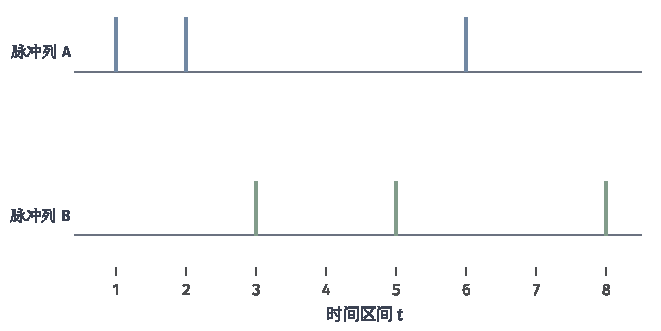
\includegraphics[width=105.412mm]{figures/05-neural-network-models/00-shared/matplotlib/snn-codes/figure.pdf}
  \caption{两条构造的脉冲列在8个等宽时间区间内都发放3次，窗口频率相同，但首次发放位置和脉冲间隔不同。竖线表示事件，横轴为时间区间编号；频率读出只保留计数，时间读出还可使用排列。}
  \label{fig:snn-codes}
\end{figure}

输入编码与输出解码不必相同。网络可以接收时间戳事件，再用输出计数分类；也可以接收持续电流，通过输出单元的首次发放作决策。输入到事件、输出到预测的两份约定共同规定了任务接口，相同观察条件下才有共同的精度与延迟口径。

\subsection{积分、泄漏与发放}
\label{sec:snn-neurons}

图~\ref{fig:snn-neuron-structure}将一个单元拆为突触响应、积分与泄漏、阈值检测和复位。输入事件只在到达时写入突触，突触响应与膜电位则保存连续值状态。输出脉冲反馈到复位路径，复位后的电位再经过一个时间步进入下一次积累；这条内部反馈使先前积累可以影响下一次响应，即使单元之间没有循环边。
\begin{figure*}[htbp]
  \centering
  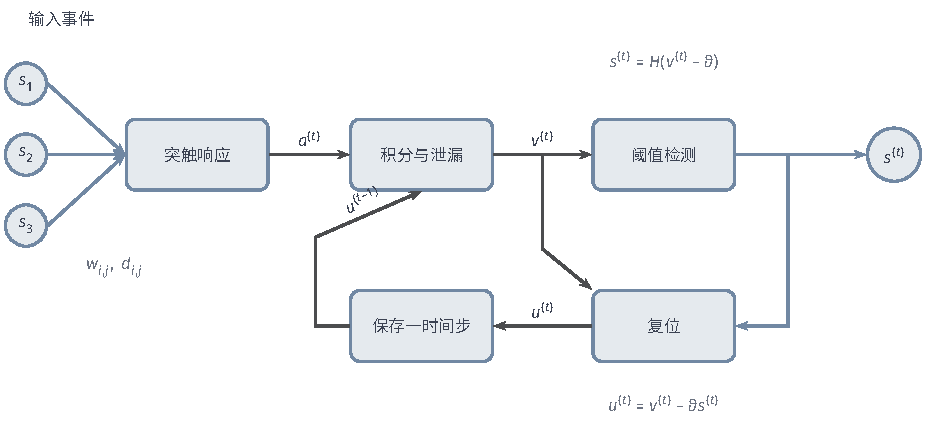
\includegraphics[width=156.792mm]{figures/05-neural-network-models/00-shared/tikz/snn-neuron-structure/figure.pdf}
  \caption{离散脉冲神经元的计算结构。输入事件经带权突触形成输入增量$a^{(t)}$，积分与泄漏模块更新复位前电位$v^{(t)}$，阈值检测模块输出脉冲$s^{(t)}$。复位模块计算电位$u^{(t)}$，下方反馈将其保存供下一步使用。图表示本章的更新次序，不表示细胞的解剖结构；突触自身也可保存状态，见式\eqref{eq:snn-synaptic-state}。}
  \label{fig:snn-neuron-structure}
\end{figure*}

一个输入脉冲通常不足以触发一次输出——否则单元只会机械地复制输入，谈不上“整合证据”。神经元真正有用的行为是：把陆续到达的输入一点点攒起来，在攒够之前保持沉默、对外只输出0，一旦积累越过某个门槛，就发出一个脉冲，然后清空（或部分清空）重新开始。同时，很久以前的输入不该和刚刚到达的输入同等重要，旧积累应当随时间慢慢淡去。为描述这套“攒—忘—发—清零”的机制，需要一个内部状态变量。\term{膜电位}（membrane potential）就是描述这种内部积累的状态变量。在简化人工模型中，膜电位相对于阈值的位置决定是否发放，这份积累还会影响下次响应。

\term{漏积分发放模型}（LIF）的名字正好概括了它的三件事：“积分”是把输入累加进膜电位，“漏”是让旧积累随时间泄漏衰减，“发放”是越过阈值时产生脉冲。它在两次发放之间用一阶动态描述积累与遗忘。设膜电位为$u_i(t)$，静息电位为$u_{\mathrm{rest}}$，输入电流为$I_i(t)$，膜时间常数为$\tau_m>0$，电阻为$R$，则
\begin{equation}
  \tau_m\frac{\mathrm d u_i(t)}{\mathrm d t}
  =-[u_i(t)-u_{\mathrm{rest}}]+RI_i(t)\text{。}
  \label{eq:snn-continuous-lif}
\end{equation}
无输入时，偏离静息电位的部分按$\exp(-\Delta t/\tau_m)$衰减。膜电位从下方达到阈值$\vartheta>u_{\mathrm{rest}}$时，模型产生一次脉冲并复位。\term{不应期}（refractory period）指发放后暂时不能再次发放的时间，可通过锁定状态或禁止发放来建模。微分方程描述两次发放之间的变化，阈值检测、复位和不应期再规定事件产生及其后的状态\scite{gerstner2014}

为便于训练，以下把静息电位移到0，并把电流及积分系数吸收到输入增量$a_i^{(t)}$中。这里的增量与膜电位具有相同单位，表示第$t$个时间区间内的输入折算到区间末端后留下的电位贡献。为了看清电流怎样变成这个量，先只考虑一个区间内没有发放的线性动态。旧电位衰减到区间末端；区间内各时刻的电流也分别积累，并按距离区间末端的时间衰减。因此，输入贡献为
\begin{equation}
  a_i^{(t)}=\frac{R}{\tau_m}
  \int_{(t-1)\Delta t}^{t\Delta t}
  \exp\!\left(-\frac{t\Delta t-\xi}{\tau_m}\right)I_i(\xi)\,\mathrm d\xi\text{。}
  \label{eq:snn-input-increment}
\end{equation}
积分中的$\xi$是连续时刻。越早到达的电流贡献经历的泄漏越久，这正是指数权重的作用。在这个区间积分的基础上，本章采用先积分、再在步末检测、再减去阈值的离散模型：
\begin{align}
  v_i^{(t)}&=\alpha u_i^{(t-1)}+a_i^{(t)},
  &\alpha&=\exp(-\Delta t/\tau_m),\label{eq:snn-discrete-integrate}\\
  s_i^{(t)}&=H(v_i^{(t)}-\vartheta),
  &H(z)&=\begin{cases}1,&z\geq0,\\0,&z<0,\end{cases}
  \label{eq:snn-discrete-fire}\\
  u_i^{(t)}&=v_i^{(t)}-\vartheta s_i^{(t)}\text{。}
  \label{eq:snn-soft-reset}
\end{align}
$v_i^{(t)}$为检测前电位，$u_i^{(t)}$为复位后电位，$\alpha\in(0,1)$控制相邻时间步之间的保留程度。此模型每步最多发放一次。若$v_i^{(t)}$远大于阈值，剩余电位会留到后面；这一单步表示因而无法记录步内可能出现的多次发放。时间步与输入尺度共同决定这项发放上限是否适合任务。

若区间内电流恒为$I_i^{(t)}$，式\eqref{eq:snn-input-increment}中的积分给出$a_i^{(t)}=R(1-\alpha)I_i^{(t)}$。例如，$\alpha=0.8$且$RI_i^{(t)}=3$时，本步输入增量为0.6；已有电位先保留原来的0.8倍，再加上这份输入。这个换算说明了输入增量与电流的关系，但步末检测仍是离散模型另作的约定，不会因区间积分精确就恢复所有步内发放时刻。人工离散网络也可以直接规定$a_i^{(t)}$，将输入尺度包含在连接权重中。后面令$\alpha=1$得到IF模型时，仍保留已规定的输入增量；这一步不再要求沿用上述有限时间常数LIF的恒流换算。

式\eqref{eq:snn-soft-reset}称为减法复位，保留超过阈值的剩余电位——它对应“一次发放只放掉恰好一个阈值那么多的电位”，因此一个很强的输入可以在后续步继续触发发放。另一种\term{硬复位}（hard reset）则更彻底，直接将发放后的电位设为$u_{\mathrm{reset}}$，即$u_i^{(t)}=(1-s_i^{(t)})v_i^{(t)}+s_i^{(t)}u_{\mathrm{reset}}$，等于每次发放后把积蓄全部清空。两种复位既改变前向轨迹，也改变反向传播。去掉泄漏、令$\alpha=1$，旧积累永不衰减，就得到离散的\term{积分发放模型}（integrate-and-fire, IF），它是后续“ANN转换”一节的理论基础；增加适应变量或非线性电位项，可以描述更丰富的发放模式。增加适应或其他动态状态，也增加相应的存储、更新与求导路径。

\begin{example}[相同输入在不同间隔下的结果]
  \label{ex:snn-integration}
  取$\alpha=0.8$、$\vartheta=1$、$u^{(0)}=0$，不设不应期。输入增量$(0.6,0.6,0,0.6)$依次给出检测前电位$(0.6,1.08,0.064,0.6512)$，输出为$(0,1,0,0)$，复位后电位为$(0.6,0.08,0.064,0.6512)$。第二步的两个近邻输入共同越过阈值，第四步到来时，先前积累已经衰减，所得电位仍在阈值下。

  若将相同的三个$0.6$改放在第1、3、5步，中间输入为0，则检测前电位依次为$0.6,0.48,0.984,0.7872,1.22976$，只有第五步发放。总输入不变，输出时刻却改变了。这组教学数值把泄漏与事件间隔的作用落实到可复算的状态轨迹。
\end{example}

图~\ref{fig:snn-lif}把示例的第一组输入画成轨迹。检测前电位用于判断发放，复位后电位成为下一步的初始状态，图中的标记也按这一次序区分。
\begin{figure}[!t]
  \centering
  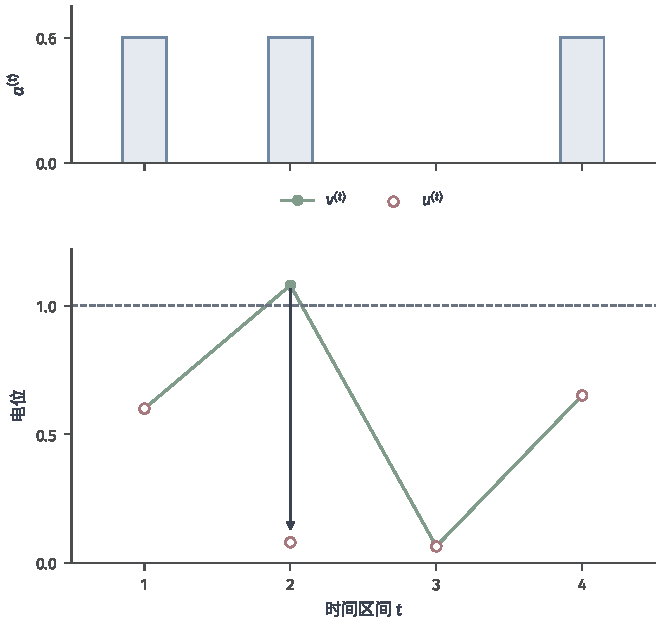
\includegraphics[width=105.412mm]{figures/05-neural-network-models/00-shared/matplotlib/snn-lif/figure.pdf}
  \caption{示例~\ref{ex:snn-integration}的离散LIF计算。蓝色柱形表示输入增量，绿色实线连接检测前电位$v^{(t)}$，红色空心圆为复位后电位$u^{(t)}$，虚线为阈值；第二步检测后发放并减去1。连线帮助比较离散状态，不表示步间的连续电位轨迹。}
  \label{fig:snn-lif}
\end{figure}

LIF保留了积累与遗忘，但它的阈值是固定不变的，这无法描述一种常见的“疲劳”现象：真实神经元在刚刚连续发放之后，往往会短暂地变得更难再次被激发，需要休息一会儿才恢复原有敏感度。固定阈值的模型只要输入不停就会一直按同一标准发放，体现不出这种自我抑制。要刻画它，可以让阈值随近期的发放历史而临时抬高，再随时间慢慢回落，这就是适应迹的作用。增加一个适应迹$r_i^{(t)}$，例如
\begin{equation}
  r_i^{(t)}=\rho r_i^{(t-1)}+s_i^{(t-1)},\qquad
  \vartheta_i^{(t)}=\vartheta_0+\kappa r_i^{(t)},
  \quad 0\leq\rho<1,\quad\kappa\geq0\text{。}
  \label{eq:snn-adaptive-threshold}
\end{equation}
这里$\vartheta_0>0$是基准阈值，$\kappa$决定适应迹对阈值的影响幅度。从无发放历史的初态开始时，可取$r_i^{(0)}=0$、$s_i^{(0)}=0$。若第$t$步发放，式\eqref{eq:snn-adaptive-threshold}会在第$t+1$步向迹中加入1；没有后续发放时，这次事件的贡献依次变为$1,\rho,\rho^2,\ldots$。当$\kappa>0$时，过去发放会暂时抬高阈值，适应迹随后衰减，阈值也逐渐回到基准。替换式\eqref{eq:snn-discrete-fire}中的阈值即可形成一种适应LIF模型。在这个示例中，复位仍按式\eqref{eq:snn-soft-reset}减去固定的$\vartheta$，可取$\vartheta=\vartheta_0$；若希望每次减去动态阈值$\vartheta_i^{(t)}$，则还需相应改变复位式。

额外状态增加了一条由$\rho$控制的发放历史通路，也增加反向路径和存储。它是否比原膜电位保留更慢的历史，要比较$\rho$与$\alpha$：在$\kappa>0$且$\rho>\alpha$时，一次发放在适应迹中的贡献比原电位的泄漏因子衰减得更慢，因而可以提供较长的响应时间尺度。若$\kappa=0$，这条迹不改变阈值；若$\rho=0$，它只保留紧邻前一步的发放。较慢的迹提供了保存历史的机制，能否据此完成需要长期信息的任务，还取决于输入、连接、学习和读出。

更复杂的神经元可以使用适应电流、非线性膜电位或离子通道状态。例如，\term{自适应指数积分发放}（adaptive exponential integrate-and-fire, AdEx）模型结合膜电位的指数非线性与适应电流。表~\ref{tab:snn-neuron-models}按状态变量与发放机制列出这些模型，使保留的细节与研究问题能够对应。
\begin{table*}[htbp]
  \centering\small
  \begin{tabularx}{\linewidth}{@{}
    >{\raggedright\arraybackslash}p{34mm}
    >{\raggedright\arraybackslash}p{49mm}
    >{\raggedright\arraybackslash}X@{}}
    \toprule
    神经元模型 & 主要状态与发放机制 & 适用关注点 \\
    \midrule
    积分发放（IF） & 膜电位积分，阈值与复位 & 简化计数对应，未包含泄漏 \\
    漏积分发放（LIF） & 膜电位积累与泄漏，阈值与复位 & 有限时间记忆与较低单元复杂度 \\
    适应LIF & 膜电位及适应迹，动态阈值或电流 & 发放历史改变后续响应 \\
    自适应指数积分发放（AdEx） & 膜电位非线性及适应电流 & 以较少状态描述丰富发放模式 \\
    Izhikevich模型 & 膜电位与恢复变量，阈值复位 & 以简化二维动态模拟多种放电行为 \\
    单室Hodgkin--Huxley & 膜电位与离子通道门控变量 & 解释动作电位产生的电流机制 \\
    \bottomrule
  \end{tabularx}
  \caption{神经元模型按保留的动态细节比较。IF与LIF还需规定复位、不应期及时间离散化；表中不计另行添加的突触和延迟状态。增加状态可以描述更多动态细节，任务预测质量则由数据、训练和相应读出评价。}
  \label{tab:snn-neuron-models}
\end{table*}
\FloatBarrier

模型细节由需要解释的响应决定。积累事件形成分类分数可以使用简化状态；研究动作电位波形或离子电流则需要能够产生这些量的动态。不同模型的参数单位、输入尺度与离散步长共同决定实际轨迹，相应数值要在各自方程中解释\scite{gerstner2014}

\subsection{网络连接与状态传播}
\label{sec:snn-connections}

图~\ref{fig:snn-connections}比较相同单元的两种组织。前馈边将事件送到下一层，每个单元的膜电位仍跨时间保留；循环边再把网络过去的发放送回当前计算。层间拓扑决定事件送往哪里，内部状态递推决定事件的影响保留多久，两者可以分别设计。
\begin{figure*}[htbp]
  \centering
  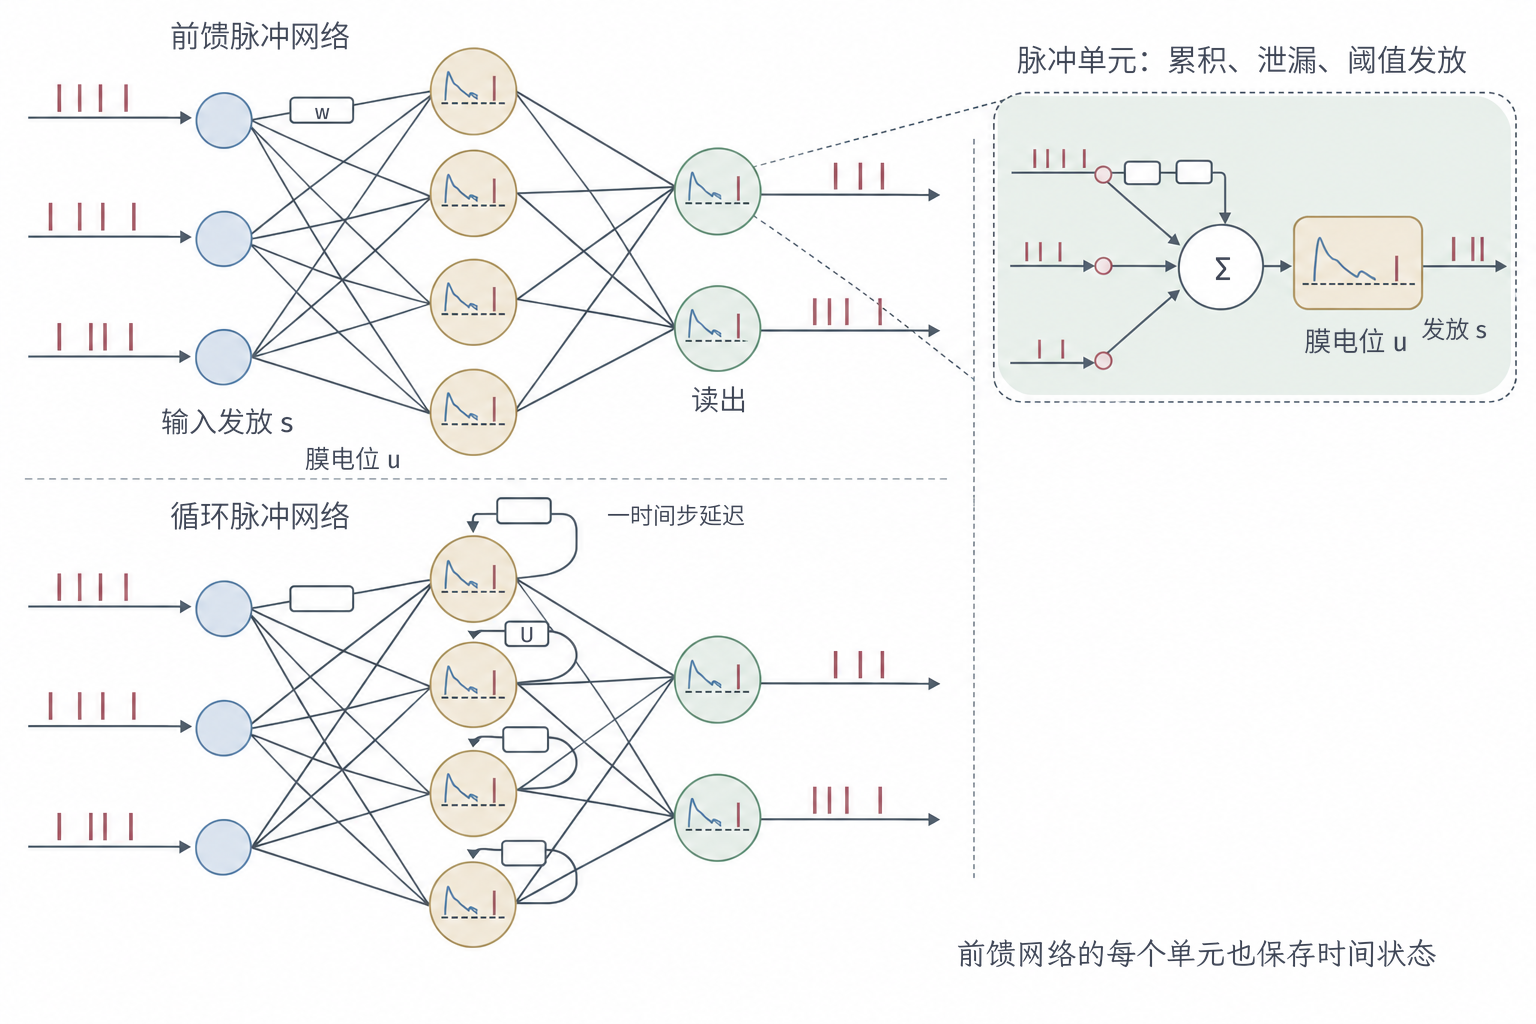
\includegraphics[width=130.048mm]{figures/05-neural-network-models/00-shared/generated/snn-connections/figure.png}
  \caption{脉冲前馈网络与循环网络的构造性比较。单元内的膜电位轨迹表示内部状态，箭头传递离散发放，右侧给出输出读出。上半部只保留层间前馈连接；下半部增加使用上一时间步脉冲的循环边$\bm U$。边还可带权重与传播延迟，图中只标出一条代表连接。神经元数和连边用于说明结构，不对应训练模型。}
  \label{fig:snn-connections}
\end{figure*}

神经元之间的连接把一个单元的发放变成其他单元的输入，这条连接在生物学上称为突触。在这里，\term{突触}（synapse）指带权连接及其对接收状态的作用，可以把它类比成前几章里带权重的连接边，但它传递的是离散事件而非连续激活。最简单的离散突触把一个到达脉冲转为电位增量$w_{i,j}$：每来一个脉冲，接收单元的膜电位就改变$w_{i,j}$这么多，正权重促使它接近阈值（兴奋性），负权重使其远离阈值（抑制性）。这里的人工模型允许同一单元的输出连接分别取正负权重。生物兴奋性、抑制性细胞对连接符号有更强约束，研究细胞类型时需将这些约束纳入模型。

为什么突触本身还需要状态？因为一个脉冲对接收细胞的影响往往不是瞬时的——生物突触释放的化学物质会让接收侧的电位在接下来一小段时间里持续变化，单个事件的作用会拖一个“尾巴”，多个事件的尾巴会叠加。要建模这种延续效应，突触就得有自己的状态变量。设一层有$m$个神经元，上层有$d$个，突触状态为$\bm q^{(t)}\in\mathbb R^m$，前馈权重为$\bm W\in\mathbb R^{m\times d}$，循环权重为$\bm U\in\mathbb R^{m\times m}$，偏置为$\bm b\in\mathbb R^m$，可写为
\begin{equation}
  \bm q^{(t)}=\beta\bm q^{(t-1)}
    +\bm W\bm s_{\mathrm{in}}^{(t)}
    +\bm U\bm s^{(t-1)}+\bm b,\qquad
  \bm a^{(t)}=\bm q^{(t)}\text{，}
  \label{eq:snn-synaptic-state}
\end{equation}
其中$\beta\in[0,1)$控制突触响应的衰减。到达脉冲写入$\bm q^{(t)}$，随后它与$\bm u^{(t)}$按各自衰减率保存历史。循环读取上一时间步的发放，使本步更新有已知输入；前馈层按层次顺序读取本步已经算出的发放。

更一般地，信号沿轴突传导需要时间，不同连接的延迟也不同，因此一个事件不一定要在下一个时间步立刻到达，可以让它“在路上走”若干步。引入延迟还有一个数学上的硬性理由：若允许零延迟的反馈环（包括自反馈），网络在同一时间步就可能出现自相矛盾的多个解，无法按确定顺序求值。令$d_{i,j}\in\{0,1,2,\ldots\}$表示边$j\to i$的总传播延迟，以离散时间步计，实际延迟为$d_{i,j}\Delta t$。权重为$w_{i,j}$的边贡献$w_{i,j}s_j^{(t-d_{i,j})}$；式\eqref{eq:snn-synaptic-state}中的前馈边对应$d_{i,j}=0$，循环边对应$d_{i,j}=1$。为保持显式更新，每个反馈回路的总延迟必须至少为一步；零延迟边组成的子图必须无环，才能按拓扑顺序读取本步已经算出的脉冲。若允许零延迟自反馈，例如$s=H(2s-1)$，则$s=0$与$s=1$都满足方程，同一历史因而允许两个本步输出，显式求值缺少唯一结果。实现还需维护尚未到达的事件队列，并为序列起点以前的脉冲指定初始历史。

脉冲前馈网络通过单元内部状态把当前响应接到历史输入上。加入循环边后，状态既保存本单元的积累，又接收其他单元的历史发放。初始状态、序列边界、延迟和同时到达事件的处理次序都属于模型定义；独立样本常重置状态，持续流则通常保留状态。

\subsection{观察时间与事件计算量}
\label{sec:snn-cost}

时间离散化和编码共同决定可表示的精度，这中间有一个绕不开的“精度—延迟”权衡。若用$K$步中的脉冲比例表示$[0,1]$内数值，能区分的最小间隔只有$1/K$：想让读数更精细，就必须观察更多步、等待更久；随机编码还叠加抽样方差。首次发放编码可以只用一个事件表示多个时间位置，理论上很快就能决策，但接收端必须一直等到该事件发生，并且要能区分事件落在哪个位置。事件较少可以降低相应通信量，较早决策则需要在更短观察时间内获得足够证据，这两者通常不可兼得。

\term{事件驱动计算}的省账方式和稠密矩阵完全不同，关键在于“只为真正发生的发放付费”。设一次推理中神经元$j$发放$N_j$次，连接到$d_j$个接收突触，若每次发放都访问这些连接，则触发的突触累加数为
\begin{equation}
  C_{\mathrm{syn}}=\sum_jN_jd_j\text{。}
  \label{eq:snn-event-cost}
\end{equation}
这个公式提醒我们：单靠“发放少”并不一定省。真正计入成本的是发放次数乘上扇出——一个单元即使很少发放，只要它的输出连接很多，每次发放仍要触发大量突触累加；反过来，一个孤立的高频单元影响的连接很少，开销也有限。除事件访问外，按时间步模拟$m$个状态单元本身还需要$O(Km)$次状态更新，因为即使没有输入，膜电位的泄漏、内部自发发放也要照算；若在通用硬件上实现为稠密矩阵乘法，未发放的那些零连接也未必会被跳过。事件驱动实现可以在到达事件时只更新相关状态，更贴合“为发生的事付费”，但它仍需额外处理泄漏、内部发放和延迟队列，工程实现并不免费。

所以，评价一个脉冲网络是否真的高效，必须算整笔账：既有事件访问，也有状态更新、延迟队列和存储管理。任务质量与决策延迟规定输出是否可用；突触访问和状态量描述成本来源，设备测量给出整条执行链的能耗。固定输入预处理与决策条件后，才能比较稀疏活动、连接组织和硬件执行各自带来的收益——这也解释了为什么在普通GPU上稠密模拟SNN常常并不省电。



\section{参数学习}
\label{sec:snn-learning}

有了网络结构，还必须解决学习问题：连接权重该怎么调，输出才能符合任务？对普通可微网络这靠反向传播，但脉冲网络里发放是阈值阶跃，在发放点不可微，这道障碍催生了三条思路截然不同、动机也各异的路线。第一条绕开梯度，直接模仿生物突触的局部规律：只用突触两端在时间上挨得近不近、谁先谁后来调整连接，不需要知道最终答案对错，也不需要全局反向传播。第二条正面迎上不可微：前向计算老老实实地用离散阶跃（保住脉冲的二值性和稀疏性），反向传播时则“善意地”把阶跃导数替换成一个光滑的替代导数，从而仍能做端到端梯度下降。第三条干脆不在脉冲网络里直接训练：先训练一个普通的连续值网络，再把它的实数激活解释成发放率，通过尺度校准转换成脉冲网络，复用已经学好的权重。三条路线使用的信息不同：局部规则根据相邻活动更新突触；端到端训练根据任务损失调整参数；转换方法先学习连续值网络，再把它的激活解释为脉冲统计量。它们可以组合使用，各条路径仍有自己的优化对象和误差来源。

下面的基本例子把泄漏、阈值和时间常数视为已给定参数，主要学习连接权重与读出。这些动态量其实也可以学习，例如用Sigmoid参数化泄漏因子、用正值变换参数化阈值，以维持模型约束；动态参数的梯度沿对应状态路径传播；整数延迟的改变则直接移动事件到达步，需要搜索或相应的可微近似。

\subsection{基于局部活动的突触学习}
\label{sec:snn-plasticity}

\subsubsection{基于共同活动的赫布更新}
\label{sec:snn-hebb-learning}

先看最简单的局部规则，它的动机是一个直观的因果联想：如果两个神经元总是在同一段时间里一起活跃，它们之间的连接多半是有用的，应当加强。这种规则完全不需要标签或全局误差，每个突触仅凭自己两端的局部信息就能更新，因而在硬件上极易分布式实现。\term{赫布学习}（Hebbian learning）根据输入端与输出端的共同活动调整连接，表达“共同活跃时加强联系”的局部相关性思想。一个简化规则为$\Delta w_{i,j}=\eta x_jy_i$，其中$x_j,y_i$是同一观察窗口的活动量，$\eta>0$为更新系数。它的隐患也很明显：持续相关活动可能令权重只增不减、无限增大，因此通常还需衰减、归一化、竞争或上下界。

\subsubsection{基于发放时间差的突触更新}
\label{sec:snn-stdp-learning}

但“共同活跃”还漏掉了因果方向。突触前（输入）先发放、突触后（输出）紧接着发放，说明前者很可能“促成”了后者，应当加强这条连接；反过来，输出已经发了、输入才到，那这次输入显然不是原因，反而应当减弱。把这种时间先后纳入权重更新，就能从单纯的相关走到带方向的因果。\term{脉冲时序依赖可塑性}（spike-timing-dependent plasticity, STDP）进一步依据突触前后发放的时间差更新权重。令$\Delta t=t_{\mathrm{post}}-t_{\mathrm{pre}}$，一种典型的成对教学规则为
\begin{equation}
  \Delta w_{i,j}=\begin{cases}
    A_+\exp(-\Delta t/\tau_+),&\Delta t>0,\\
    -A_-\exp(\Delta t/\tau_-),&\Delta t<0,
  \end{cases}
  \label{eq:snn-stdp}
\end{equation}
其中$A_+,A_->0$为幅度，$\tau_+,\tau_->0$为时间尺度，同时发放时另定规则。该形式把“输入先到、输出随后发生”与相反次序区分开。生物实验中的权重变化还随细胞类型、突触强度和发放组合改变\scite{bi1998}

局部计算不必保存所有事件对。可以用指数衰减的活动迹记录近期发放，突触后发放时读取突触前迹来加强权重，突触前发放时读取突触后迹来减弱权重。采用所有配对还是最近邻配对、权重是否有界，会产生不同学习动态。

\subsubsection{用任务信号调制局部更新}
\label{sec:snn-modulated-learning}

局部规则有个根本缺陷：它衡量的只是“两个单元是否经常一起发”，这与“它们是否有助于答对任务”是两回事——经常同时出现的输入可能只是背景噪声，真正区分类别的特征反而不那么频繁。要弥合这道鸿沟，需要让最终的任务结果（奖励或误差）也参与更新，哪怕它比局部事件晚到很久。生物大脑里多巴胺等神经调质正是扮演这种“全局广播的奖惩信号”：突触先把“我刚才活动过”记成一笔会随时间消退的账，等奖励到来时再据此决定加强还是减弱。为把局部活动与任务结果连接，可加入第三个调制信号，令$\Delta w_{i,j}=\eta m^{(t)}e_{i,j}^{(t)}$。其中$e_{i,j}^{(t)}$是记录近期局部活动及可更新程度的\term{资格迹}（eligibility trace），$m^{(t)}$传递奖励、误差或其他全局调制。迹保存的是哪些突触近期发生了可参与更新的活动，调制信号再决定这些活动应引起怎样的权重变化。第三因素由此把任务结果接到近期局部活动上，也允许任务信号比局部事件更晚到达。

第\ref{chap:neural-network-overview}章已经说明局部活动可以先留痕迹、等待奖励到来；现在可以把这段时间关系接到更新式上。作为一个示意构造，设$g_{i,j}^{(t)}$为第$t$步由突触两端活动形成的局部量，例如成对发放产生的带符号更新量，令
\begin{equation}
  e_{i,j}^{(t)}=\lambda_e e_{i,j}^{(t-1)}+g_{i,j}^{(t)},
  \qquad 0\leq\lambda_e<1\text{。}
  \label{eq:snn-eligibility-example}
\end{equation}
这里$\lambda_e$决定痕迹保留多久。假设第1步结束时迹为0，即$e_{i,j}^{(1)}=0$，第2步的局部活动使$g_{i,j}^{(2)}=1$，其后到第5步都没有新的局部量，那么第5步仍有$e_{i,j}^{(5)}=\lambda_e^3$。若任务调制此时到达，该步权重变化为$\eta m^{(5)}\lambda_e^3$。局部事件发生时先记录，之后逐步衰减，较晚的任务结果再读取尚存的迹；这三步解释了更新式怎样连接先前活动与后来结果。具体学习规则可以采用不同的资格迹，式\eqref{eq:snn-eligibility-example}只展示保留和调制的分工。只有相应调制信号与资格迹构造给出目标梯度时，才能据它作梯度下降分析\scite{gerstner2018plasticity}

\subsection{基于替代梯度的端到端学习}
\label{sec:snn-surrogate}

\subsubsection{离散发放的反向信号}
\label{sec:snn-surrogate-signal}

局部规则虽然省、也贴近生物，但它没有直接优化任务损失，难以和前几章成熟的深度训练接轨。最直接的监督学习做法，是像RNN一样把网络沿时间展开、用输出误差对所有连接做反向传播。先规定输出怎么读：设每个样本含$K$步输入脉冲，标签为$y$，输出读出为$\bm z=K^{-1}\sum_t\bm s_{\mathrm{out}}^{(t)}$，即统计输出单元在整段时间的平均发放率，可以用$\ell(\bm z,y)$训练分类器。膜电位、过滤状态或发放时间也可以形成预测；所选读出决定误差从哪些输出与时刻进入网络。

真正的拦路虎是式\eqref{eq:snn-discrete-fire}里的阶跃函数$H$：它在阈值以下和以上的普通导数都是0，只在阈值那一点跳变。如果老老实实地把这个导数代入链式法则，会发生两件糟糕的事——绝大多数位置的梯度都是0，误差根本传不回去，无法调整参数；而当某个参数只变一点点、让膜电位恰好跨过阈值时，输出又会从0突然跳到1，整条时间轨迹随之突变。\term{替代梯度}（surrogate gradient）用一个“前向照实、反向做手脚”的办法绕开它：前向计算中保留离散发放（输出仍是真实的0/1，保住脉冲的全部性质），在反向计算中则用一个有限、非零的光滑函数代替阶跃导数，给梯度开一条可通行的路。例如，令$z=v-\vartheta$，使用
\begin{equation}
  \frac{\partial s}{\partial v}\ \rightsquigarrow\
  \psi(z)=\frac{c}{(1+\kappa|z|)^2},\qquad c,\kappa>0\text{。}
  \label{eq:snn-surrogate-derivative}
\end{equation}
符号$\rightsquigarrow$标出反向所采用的规则，它与前向阶跃的普通导数承担不同角色。在固定$c$和$\kappa$时，$\psi$在阈值附近取较大的值，离阈值越远则越小。回传到电位的信号还要乘以从后续计算传来的误差；在其余回传量相同时，较大的局部替代系数才使这条路径保留较大的信号幅值。若后续传来的误差为0，即使电位靠近阈值，这条路径也没有回传贡献。因此，这里比较的是局部因子，不能仅按阈值距离判断完整参数梯度的大小。$c$改变梯度幅度，$\kappa$改变有效宽度；两者与阈值及电位尺度有关\scite{neftci2019surrogate}

替代规则也进入复位的导数。对本章的减法复位，若不停止复位路径的求导，有
\begin{equation}
  \frac{\partial u_i^{(t)}}{\partial v_i^{(t)}}
  \ \rightsquigarrow\ 1-\vartheta\psi(v_i^{(t)}-\vartheta)\text{。}
  \label{eq:snn-reset-gradient}
\end{equation}
若实现中把复位脉冲视为常数，这个导数改为1。两种约定共享前向轨迹，却给历史状态分配不同的回传信号；硬复位也按自身表达式产生另一组导数。复位路径的选择与发放处的替代函数共同组成训练规则。

图~\ref{fig:snn-surrogate-forward-backward}将真实前向发放与指定的反向规则放在同一计算链上。两种复位导数约定共享前向状态更新，区别只进入回传。

\begin{figure*}[htbp]
  \centering
  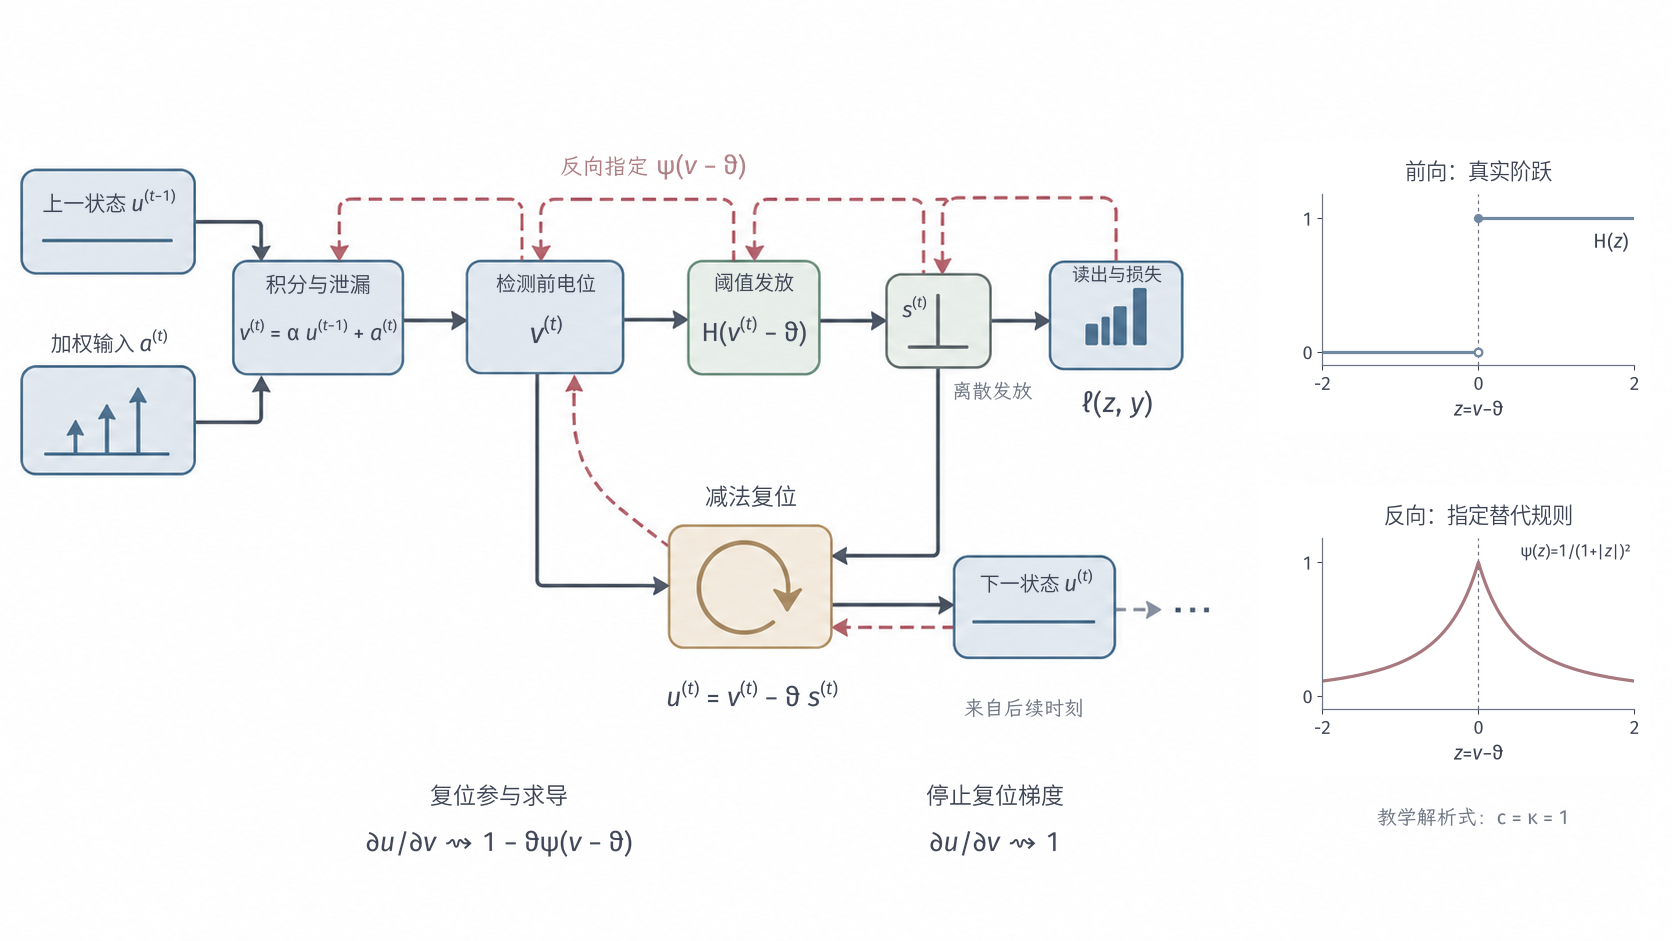
\includegraphics[width=141.563mm]{figures/05-neural-network-models/00-shared/generated/snn-surrogate-forward-backward/figure.png}
  \caption{LIF前向计算与替代梯度。前向使用真实阶跃发放和减法复位；反向在发放处指定替代规则$\psi$。右侧解析曲线取$c=\kappa=1$，阶跃在零处取一；下方两式分别表示复位参与求导与停止复位梯度，两种约定不改变前向发放。}
  \label{fig:snn-surrogate-forward-backward}
\end{figure*}

\subsubsection{沿时间展开分配任务误差}
\label{sec:snn-unrolled-training}

将$\bm q^{(t)}$、$\bm u^{(t)}$和所需延迟状态合并为$\bm h^{(t)}$，网络可写为$\bm h^{(t)}=F_{\bm\theta}(\bm h^{(t-1)},\bm x_t)$。这里$\bm h^{(t)}$表示第$t$步结束后保存的状态，包括供下一步读取的本步发放$\bm s^{(t)}$以及尚未到达的事件；更新第$t$步时，读取的则是$\bm h^{(t-1)}$中保存的历史。把这一递推展开到各个时间步，再累积所有调用同一参数的贡献，就得到第\ref{chap:recurrent-networks}章的时间反向传播；发放与复位处使用上述指定导数。

可以先沿一条膜电位路径看这种回传怎样发生。固定本步输入增量$a_i^{(t)}$、泄漏因子和阈值，只追踪$u_i^{(t-1)}\to v_i^{(t)}\to u_i^{(t)}$：旧电位先乘$\alpha$进入积分，再经过减法复位。将式\eqref{eq:snn-discrete-integrate}的局部系数与式\eqref{eq:snn-reset-gradient}相乘，这条直接路径的反向系数为
\begin{equation}
  \left.\frac{\partial u_i^{(t)}}{\partial u_i^{(t-1)}}\right|_{a_i^{(t)}\,\mathrm{fixed}}
  \ \rightsquigarrow\
  \alpha\left[1-\vartheta\psi(v_i^{(t)}-\vartheta)\right]\text{。}
  \label{eq:snn-membrane-backward-path}
\end{equation}
若停止复位脉冲的求导，这条路径的系数就变为$\alpha$。在更长的展开图中，同一路径沿时间继续传递时，会依次乘上各步相应的系数；循环突触、输出读出和其他状态还会形成额外路径，其贡献需要在汇合处相加。因此，式\eqref{eq:snn-membrane-backward-path}只展示直接膜状态路径，不是整个网络状态的完整雅可比。各时间步重复调用同一权重，最后仍须把这些调用位置对该权重的贡献累积起来。

在保存前向激活的实现中，较长窗口需要保存更多状态，重算可以改变这份存储代价；截断展开则删除相应历史梯度路径。所得回传信号由整套替代规则定义，其下降行为需要结合实际离散损失检验；对统一平滑目标作优化分析，还需另行建立这种规则与目标梯度的关系。

\begin{algorithm}[脉冲网络的监督训练]
  \label{alg:snn-supervised}
  \begin{algorithmic}[1]
    \Require 输入序列与标签、时间步数$K$、神经元参数、替代规则$\psi$
    \Ensure 学得的权重与读出参数
    \For{每个训练小批量}
      \State 按样本边界设置膜电位、突触状态和延迟队列
      \For{$t=1,\ldots,K$}
        \State 计算突触输入，按式\eqref{eq:snn-discrete-integrate}--\eqref{eq:snn-soft-reset}更新各层
        \State 保存反向计算所需状态并积累输出读出
      \EndFor
      \State 由读出与标签计算损失
      \State 沿展开图反向计算，以$\psi$代替发放导数并采用约定的复位导数
      \State 累积共享参数梯度，必要时裁剪，再更新参数
    \EndFor
  \end{algorithmic}
\end{algorithm}

\subsection{基于连续值网络的参数转换}
\label{sec:snn-conversion}

\subsubsection{连续激活与发放率的对应}
\label{sec:snn-rate-conversion}

第三条路线的动机很实际：替代梯度虽然能训，但脉冲网络仍然比普通网络难训得多、精度常常差一截，而连续值网络经过多年发展已有成熟的训练方法和大量高精度模型。能不能先把连续网络训到最好，再“无损地”搬到脉冲硬件上运行？这就需要建立一座桥梁：把连续网络里某个单元的实数激活，解释成脉冲单元在一段时间里的平均发放率——激活越大，对应单元发放越频繁；只要观察窗口足够长，发放率就能逼近那个实数。\term{人工网络到脉冲网络转换}（ANN-to-SNN conversion）就是建立连续激活与脉冲统计量的对应，以复用已经学得的权重。这座桥为什么成立、误差又从哪里来，可以从不泄漏的积分发放模型看起。

设$\alpha=1$、$u^{(0)}=0$，采用减法复位，每步输入增量为$a^{(t)}$，将$K$次状态更新求和得
\begin{equation}
  \vartheta\sum_{t=1}^{K}s^{(t)}
  =\sum_{t=1}^{K}a^{(t)}-u^{(K)}\text{。}
  \label{eq:snn-conversion-balance}
\end{equation}
若输入非负且每步不超过$\vartheta$，则$0\leq u^{(K)}<\vartheta$，于是
\begin{equation}
  0\leq\frac1K\sum_{t=1}^{K}a^{(t)}
       -\frac{\vartheta}{K}\sum_{t=1}^{K}s^{(t)}
  <\frac{\vartheta}{K}\text{。}
  \label{eq:snn-conversion-error}
\end{equation}
这说明阈值乘以平均发放量可以近似平均输入，剩余电位造成有限窗口误差。比如恒定输入0.3、阈值1、窗口4步，只发放1次，对应平均值0.25，尚有0.2电位未释放。窗口10步恰好发放3次，对应0.3。该界控制已校准单元的剩余电位误差；多层网络还会接受上游发放形成的新输入。

\subsubsection{层间尺度校准与转换误差}
\label{sec:snn-conversion-calibration}

实际转换需处理负激活、偏置、归一化和不同层的尺度。先把推理时已经固定的仿射运算合并，再确定每层的连续激活由多大的发放比例表示，才能把单元的平均输入关系接到整个网络。

对线性层$\bm W\bm x+\bm b$，若训练后的BatchNorm使用固定均值$\mu$和方差$\sigma^2$，它的仿射变换可以折叠到权重与偏置。具体地，对输出通道$i$，设$z_i=\bm W_{i,:}\bm x+b_i$，推理时的BatchNorm输出为
\[
  \begin{aligned}
    &\gamma_i\frac{z_i-\mu_i}{\sqrt{\sigma_i^2+\epsilon}}+\zeta_i\\
    &\qquad=\frac{\gamma_i\bm W_{i,:}}{\sqrt{\sigma_i^2+\epsilon}}\bm x
       +\frac{\gamma_i(b_i-\mu_i)}{\sqrt{\sigma_i^2+\epsilon}}+\zeta_i\text{。}
  \end{aligned}
\]
将乘输入的系数与常数项分别合并，就有
\begin{equation}
  \bm W'_{i,:}=\frac{\gamma_i\bm W_{i,:}}{\sqrt{\sigma_i^2+\epsilon}},\qquad
  b'_i=\frac{\gamma_i(b_i-\mu_i)}{\sqrt{\sigma_i^2+\epsilon}}+\zeta_i\text{。}
  \label{eq:snn-bn-folding}
\end{equation}
这里$\gamma_i,\zeta_i$为归一化的缩放和偏移，$\epsilon>0$是分母中的稳定项，折叠使用推理统计量。固定统计量后，这一步只是同一个仿射映射的代数重写；若均值和方差还随当前训练小批量变化，就不能用同一组固定参数代表所有小批量。

合并仿射运算后，仍需处理激活单位。考虑一个ReLU层，记其有效权重与偏置为$\bm W_l,\bm b_l$；若原网络含上述BatchNorm，这里使用的就是折叠后的参数。该层计算$\bm h_l=\operatorname{ReLU}(\bm W_l\bm h_{l-1}+\bm b_l)$。取每层正尺度$\lambda_l>0$，用$\widetilde{\bm h}_l=\bm h_l/\lambda_l$表示归一化激活。单步最多发放一次，平均发放量只能位于$[0,1]$，所以需要让有代表性的激活大部分落在这一范围内。前一层的单位也随之改变：$\bm h_{l-1}=\lambda_{l-1}\widetilde{\bm h}_{l-1}$。

对于任意$c>0$，ReLU满足$\operatorname{ReLU}(c\bm z)=c\operatorname{ReLU}(\bm z)$。将前一层的单位关系代入本层，再把正因子$1/\lambda_l$按这个等式移入ReLU，可得
\begin{align}
  \widetilde{\bm h}_l
  &=\frac{1}{\lambda_l}\operatorname{ReLU}
       \bigl(\lambda_{l-1}\bm W_l\widetilde{\bm h}_{l-1}+\bm b_l\bigr)\notag\\
  &=\operatorname{ReLU}
       \left(\frac{\lambda_{l-1}}{\lambda_l}\bm W_l\widetilde{\bm h}_{l-1}
              +\frac{\bm b_l}{\lambda_l}\right)\text{。}
  \label{eq:snn-layer-scale-identity}
\end{align}
因此，相邻两层的尺度要共同进入权重，偏置则按本层输出尺度换算：
\begin{equation}
  \widetilde{\bm W}_l=\frac{\lambda_{l-1}}{\lambda_l}\bm W_l,\qquad
  \widetilde{\bm b}_l=\frac{\bm b_l}{\lambda_l}\text{。}
  \label{eq:snn-layer-scale-parameters}
\end{equation}
只缩小本层权重而不处理输入单位和偏置，一般会改变原网络计算的函数。式\eqref{eq:snn-layer-scale-identity}说明了怎样在连续网络中保留原函数的尺度对应，还没有涉及有限窗口的脉冲近似。

接下来才把归一化激活解释为平均发放量。在无泄漏、减法复位、单位阈值的基本转换中，可用到达脉冲形成每步增量
\begin{equation}
  \bm a_l^{(t)}=\widetilde{\bm W}_l\bm s_{l-1}^{(t)}
                      +\widetilde{\bm b}_l\text{。}
  \label{eq:snn-converted-input}
\end{equation}
这里直接使用当前到达事件，不额外加入突触滤波。偏置作为每步恒定输入进入积分，因此对$K$步取平均后仍是$\widetilde{\bm b}_l$；若只在窗口开始时加一次，平均贡献就会缩小为$\widetilde{\bm b}_l/K$。上游平均发放若接近$\widetilde{\bm h}_{l-1}$，本层的平均输入就接近$\widetilde{\bm W}_l\widetilde{\bm h}_{l-1}+\widetilde{\bm b}_l$。对满足式\eqref{eq:snn-conversion-error}条件的单元，再由输入与发放之间的余量关系控制本层的有限窗口偏差。

例如，一个教学单通道层计算$h=\operatorname{ReLU}(2x+1)$，取输入$x=3$、前一层尺度4和本层尺度10。原输出为7，归一化输入为0.75，归一化输出为0.7。按式\eqref{eq:snn-layer-scale-parameters}换算，权重变为$2\times4/10=0.8$，偏置变为$1/10=0.1$，于是$\operatorname{ReLU}(0.8\times0.75+0.1)=0.7$。若上游脉冲比例为0.75，每步输入为$0.8s^{(t)}+0.1$，平均输入便为0.7。这个平均量仍不等于任意有限窗口的输出脉冲比例：窗口只有4步时，比例只能以0.25为间隔变化，不能恰好读出0.7，差别会留在末电位中。

阈值或层权重再依据代表性校准数据调节，使常见激活既不会长期静默，也不会超出单步发放上限。上述正尺度换算给出一种具体做法：尺度过大，会把激活压到很低的比例，有限窗口内可能难以形成足够发放；尺度过小，则可能要求超过每步一次的发放量。校准数据决定了重点保留哪一段激活范围，超过这一范围的新输入仍可能饱和\scite{rueckauer2017conversion}

层间换算还要保留单元误差界的条件。ReLU激活非负，不代表带负权重或负偏置的逐步输入增量始终非负；若输入变负，或单步增量超过阈值，式\eqref{eq:snn-conversion-error}所用的余量区间就不再自动成立。负激活也不能直接由非负脉冲计数表示，需要另行选择符号编码或改变待转换的模型。层尺度的代数对应、逐步输入的实际范围和有限窗口的发放误差由此是三个需要分别核对的环节。

加入泄漏后，式\eqref{eq:snn-conversion-balance}会多出遗忘项；采用硬复位还会丢弃超阈值的剩余电位。多层的有限窗口误差、上游发放延迟和统计尺度偏差都可能累积。转换适合能够由非负发放统计量近似的计算。目标若使用精确相对时序，编码与动态还需保留这份时间差；端到端脉冲训练可以直接在目标窗口和读出上调整参数。
\Needspace{8\baselineskip}
\section{理论分析}
\label{sec:snn-analysis}

学完结构和训练方法，还应冷静回答三个层层递进的问题，它们与前面各章的理论框架完全一致。第一，表达能力：给定编码、状态和读出，脉冲网络的候选函数里到底有没有我们想要的映射？尤其要追问，时间信息在“编码—状态—读出”这条链路上是否会在某一环被彻底丢掉。第二，收敛性：替代梯度这种“前向真实、反向替换”的做法，还能不能套用普通梯度下降的收敛结论？第三，泛化性：在一段事件记录上学到的规律，能否推广到没见过的新记录？由于阈值发放不连续，这三问的答案都比连续网络更依赖具体条件，结论也要相应收窄。

\subsection{表达能力}
\label{sec:snn-temporal-stability}

判断脉冲网络能否区分两类输入，必须沿整条链路逐环检查，任何一环把差别抹掉，后面就再也找不回来。先看编码：若编码只给出窗口内的脉冲计数，那么原始的时间顺序在入口处就已经丢失，后续网络再强也无法从计数还原排列。再看状态：即使编码保留了时刻，若膜时间常数太短，相隔很远的两个事件也可能互不影响、无法建立联系。最后看读出：即使网络内部确实形成了不同状态，若最终只对所有发放做一次总计数，两条不同轨迹仍可能被合并成同一个数。编码保留下来的差别，经过状态和读出后是否仍可辨认，才决定整个映射的表达能力。

\begin{theorem}[无泄漏积分发放单元的数值逼近精度]
\label{thm:snn-rate-approximation}
设输入为任意$a\in[0,1]$，每步输入增量均为$a$。单元采用$\alpha=1$、阈值$1$、零初态和减法复位，每步最多发放一次。观察$K\geq1$步，令$N_K$为总发放次数，则
\[
 N_K=\lfloor Ka\rfloor,\qquad
 0\leq a-\frac{N_K}{K}<\frac1K\text{。}
\]
因此该编码与读出对任何支撑在$[0,1]$上的输入分布，都有不超过$1/K$的$L^p$逼近误差，$1\leq p\leq\infty$。
\end{theorem}
\begin{proof}
$a\leq1$使每次复位后的电位始终在$[0,1)$内。将$u^{(t)}=u^{(t-1)}+a-s^{(t)}$相加，得到$u^{(K)}=Ka-N_K\in[0,1)$，即得结论。
\end{proof}
这是频率读出对连续强度的明确表示结论，观察窗口越长，最坏误差越小。它只针对无泄漏的单元，不保证任意深层LIF网络都按同样速度逼近目标。

仅用计数还会丢失顺序：输入脉冲$(1,0)$与$(0,1)$有相同计数。若整个候选只读取计数，目标却在这两条序列上分别取$0$和$1$，任意候选的最大绝对逼近误差至少为$1/2$。需要区分先后时，必须保留事件时刻或能区分两条轨迹的内部状态。

\subsection{收敛性}
\label{sec:snn-convergence}

这里首先要区分两件常被混为一谈的事：训练目标“最小值是否存在”，与梯度下降“能否收敛、多快收敛”。前者是优化问题本身有没有解，后者是算法能不能找到它，二者的条件在脉冲网络里都因硬阈值而变得更微妙。硬阈值使参数到脉冲输出的映射可能不连续——参数的微小变化一旦让某个膜电位跨过阈值，输出会整体跳变。即使参数域是紧的，连续目标那种最小值一定存在的论证也不能直接用于它。一个保底的存在性结论来自有限性：若架构、观察窗口和允许的参数取值均预先固定且候选有限，经验目标一定在某个候选处取得最小值；理论上枚举就能求解，但候选数可能随参数量化位数指数增长，并无实用价值。

\begin{theorem}[脉冲网络可微松弛光滑目标的驻点收敛速度]
\label{thm:snn-stationary-rate}
固定训练集、网络结构和确定性的前向计算，记使用连续发放函数替代硬阈值后、完整可微前向计算的全批量训练目标为$J(\bm\theta)$。假设$J\geq J_{\inf}$，且梯度在包含迭代点及更新线段的区域内为$\beta$-Lipschitz，其中$\beta>0$。采用完整梯度下降
$\bm\theta^{(k+1)}=\bm\theta^{(k)}-\eta\nabla J(\bm\theta^{(k)})$，步长满足$0<\eta\leq1/\beta$。对任意$K\geq1$，
\begin{equation}
 \frac1K\sum_{k=0}^{K-1}\lVert\nabla J(\bm\theta^{(k)})\rVert_2^2
 \leq\frac{2[J(\bm\theta^{(0)})-J_{\inf}]}{\eta K}\text{。}
 \label{eq:snn-stationarity-rate}
\end{equation}
对任意$\varepsilon>0$，至少有一个已计算迭代点的梯度范数不超过$\varepsilon$，只需
$K\geq2[J(\bm\theta^{(0)})-J_{\inf}]/(\eta\varepsilon^2)$。
\end{theorem}
证明与定理~\ref{thm:ffn-stationary-rate}相同：沿完整计算图求出梯度，使用下降引理并对更新次数求和。

该界回答了接近一阶驻点需要多少次更新。它不保证驻点是全局最小点，也不保证参数序列存在唯一极限。若还满足$\lVert\nabla J\rVert_2^2\geq2\mu(J-J_*)$，其中$\mu>0$、$J_*$为最小值，再限制$\eta\leq1/\mu$，则有
$J(\bm\theta^{(K)})-J_*\leq(1-\eta\mu)^K[J(\bm\theta^{(0)})-J_*]$。这一条件需要对具体训练问题验证，不能由网络名称推得。

上一定理只适用于真正的可微松弛目标，而且更新必须使用该目标的精确梯度。常见替代梯度训练保留硬阈值前向计算，却人为替换反向导数，所得方向未必是原任务目标或某个松弛目标的梯度。因而不能把上面的驻点速度直接写成硬脉冲网络的训练保证。目前本章没有给出对所述硬阈值、减法复位与替代梯度组合普遍成立的目标下降或全局收敛结果。

固定发放模式下，相同输入驱动的LIF状态差可以按泄漏因子衰减；阈值切换则可能改变发放与复位。这解释了局部状态响应，不等于参数训练收敛。固定脉冲储备池上的岭读出属于定理~\ref{thm:rnn-reservoir-readout-convergence}的凸二次情形，结论仅覆盖读出。

\subsection{泛化性}
\label{sec:snn-generalization}

连续网络的泛化界通常建立在“模型对参数连续、可以用参数邻域覆盖候选”之上；硬阈值恰好破坏了这种连续性——参数的无穷小变化都可能翻转一次发放，Lipschitz条件无从谈起。但换一个角度反而好办：如果预先把每个系数限制为有限个离散取值（神经形态硬件上参数本来就常常是低比特量化的），整个模型族的候选数就是有限的，泛化分析只需数清楚有多少个候选，不必再依赖可微性。把一个完整事件记录及其标签视为样本，固定编码、观察窗口、初态和读出。阈值跳变使连续参数覆盖的Lipschitz条件难以直接使用；预先限制参数取值则可绕过这一障碍，给出明确的有限候选风险保证。

\begin{theorem}[有限精度脉冲网络在独立记录上的期望风险界]
\label{thm:snn-finite-risk}
固定脉冲网络结构、编码、观察窗口、复位和确定性预测规则，共有$p$个可调系数，每个系数的预定取值不超过$2^b$种。损失可测且在$[0,1]$内，包括固定平局规则下的零一分类损失。训练集$S$含$n$个独立同分布的完整事件记录。记期望风险为$R$、经验风险为$\widehat R_S$。对任意$\delta\in(0,1)$，以至少$1-\delta$的概率，任意候选内训练输出$\widehat f$满足
\[
 R(\widehat f)\leq\widehat R_S(\widehat f)
 +\sqrt{\frac{pb\log2+\log(2/\delta)}{2n}}\text{。}
\]
若训练的经验优化误差至多为$\xi$，还满足
\[
 R(\widehat f)\leq\inf_f R(f)
 +2\sqrt{\frac{pb\log2+\log(2/\delta)}{2n}}+\xi\text{。}
\]
\end{theorem}
证明与定理~\ref{thm:cnn-quantized-risk}相同。有限候选计数不要求阈值可微，因此能够覆盖这里指定的硬发放模型；训练算法只要输出候选内模型，第一条界就成立。第二条界另需经验优化误差的条件，替代梯度不自动保证$\xi$很小。

该界通常较粗，参数位数与规模很大时可能只有平凡保证。它不支持任意连续权重，也不覆盖无界损失。目前本章没有给出一般连续参数、硬阈值脉冲网络的更精细直接期望风险结果。窗口变长不增加独立记录数；同一连续流的重叠窗口又可能相关。训练和部署采用不同窗口、编码阈值或设备时，分布及预测过程可能改变，必须重新规定风险条件。

\section{常见应用}
\label{sec:snn-applications}

本章的概念最终要落到两类任务上：一类输入本身就是离散事件流（如事件相机的手势识别），SNN可以直接消费；另一类输入是连续不断到来、没有明确终点的感知流（如持续监测和运动响应），关键在于如何带着状态实时处理、并在恰当时刻输出。下面各举一个代表性场景，重点看清前面的编码、状态累积和读出在完整预测路径中如何各司其职。

\subsection{事件流识别}
\label{sec:snn-event-recognition}

变化驱动的视觉传感器为脉冲网络提供了最自然的直接输入。\term{事件相机}（event camera）在像素亮度变化达到阈值时输出位置、时刻和变化方向，而非在固定间隔输出整帧图像。一个样本可表示为事件序列$\{(x_k,y_k,t_k,p_k)\}_{k=1}^{n_e}$，其中$(x_k,y_k)$为像素坐标，$t_k$为时间戳，$p_k\in\{-1,1\}$为亮度变化极性。这些观测记录的是亮度变化这一“增量”；要恢复绝对亮度还需要初始信息或相应重建过程\scite{lichtsteiner2008sensor}

以动作片段分类为例，可以按像素和极性分输入通道，将时间戳划入宽度$\Delta t$的区间，得到输入脉冲张量。如果同一像素在一个区间多次触发，可采用事件计数，或缩短区间以保留二值表示；合并事件会改变信息。空间卷积连接提取局部变化模式，膜电位与突触状态累积时间关系，再用类别输出单元的计数或连续读出产生分数。

若类别$c$的计数为$N_c$，可以取$z_c=N_c/K$并用Softmax交叉熵训练，预测为$\argmax_c z_c$；所有计数为0时要规定平局处理或继续观察。损失可以只在片段结束计算，也可以在多个截断窗口计算以训练较早输出。在固定评价时刻比较输出，可以保持可用事件范围一致；多个窗口的监督则让模型在不同证据量下练习决策。

同一记录的相邻窗口往往共享动作、场景和事件，分散到训练与测试会让评价重复看到相关证据。按独立片段、主体或场景划分数据，才与相应新数据问题匹配；事件噪声与传感器阈值变化也要在规定的时间预算下评价。

\subsection{连续感知与动态响应}
\label{sec:snn-continuous-response}

持续感知没有天然的片段终点。网络接收不断到来的变化，保留状态，并在预定时刻或满足决策条件时产生输出。例如，一个教学运动方向检测器可用两组位置通道接收事件，再设置不同突触延迟，使某一方向依次到达的事件在下游重合；反向事件到达时没有同样的同步积累。LIF的积累与阈值把这种重合转为发放，方向读出据此给出分数。

连续输出也可以从过滤后的状态得到。设$m$维输出脉冲为$\bm s^{(t)}$，令$\bm r^{(t)}=\rho\bm r^{(t-1)}+(1-\rho)\bm s^{(t)}$，$\rho\in[0,1)$，再用$\hat{\bm y}^{(t)}=\bm C\bm r^{(t)}+\bm d$预测连续量。$\rho$越大，输出越平滑，也越迟缓；用膜电位读出则会保留阈值以下的状态。过滤参数与读出方式共同确定响应速度和抖动，任务评价据这份实际输出进行。

持续状态还会带来边界问题。静默期间应让历史影响按模型衰减；传感器重启、场景切换或长时间中断后，可以按明确规则重置状态。训练时若每个短窗口都重置，使用时却无限保留状态，网络面对的状态分布可能不同。跨窗口保留状态让早期输入继续影响预测，截断的梯度却不再把后来误差送回对应的早期计算；记忆长度与误差回传长度由此可以不同。

\section{本章小结}
\label{sec:snn-summary}

SNN把到达事件写入连续状态，以积累、泄漏、阈值和复位产生后续发放，再由读出形成预测。先后关系可以通过状态和延迟保留，计数也可以近似输入强度；编码与读出共同决定哪些差别留到输出。局部活动规则、指定的替代梯度与连续网络转换分别提供不同学习信号，训练结果据实际离散预测检验。窗口更长可降低特定编码误差，同时增加等待、事件访问和状态更新；事件稀疏性带来的收益由整条输入到设备的链路决定。

\paragraph{扩展阅读}
Gerstner等的教材从膜电位、发放与突触可塑性建立神经元动力学。其中的连续动态与本章离散更新相接，突触可塑性又为局部学习提供来源；替代梯度和转换方法则对应人工任务中的两种训练路径。观察窗口、决策延迟与设备执行把这些模型接到实际事件计算\scite{gerstner2014}

\chapter{神经网络的训练}
\label{chap:neural-network-training}

同一网络用较大步长更新时可能在谷底两侧振荡，用较小步长又可能长时间停留在高损失区。增加批量会改变梯度噪声，增加层数或序列长度还会改变误差传回早期参数的路径。反向传播给出当前位置的梯度，训练还需决定怎样使用它。目标的局部形状、估计的精度与网络的信息传播，共同决定这一步更新能产生什么进展。

各模型的求导过程已经把损失接到可训练参数上。这里将这些参数放入共同的更新过程：优化器读取梯度与历史，决定参数增量；表示尺度、连接和参数化再决定梯度怎样形成。它们可以共同使用，各自的作用沿这条计算链解释。降低训练误差需要更新找到有用的候选，这个候选在新数据上的表现则由第\ref{chap:neural-network-generalization}章分析。

设训练集为$\{(\bm x_i,y_i)\}_{i=1}^n$，所有可训练参数展平为$\bm\theta\in\mathbb R^p$，经验目标为
\begin{equation}
  \mathcal L(\bm\theta)=\frac1n\sum_{i=1}^n
  \ell(f_{\bm\theta}(\bm x_i),y_i)\text{。}
  \label{eq:training-objective}
\end{equation}
这里$p$是参数数目，$n$是样本数。第$t$次更新在$\bm\theta^{(t-1)}$处计算梯度或其估计$\bm g^{(t)}$，再得到$\bm\theta^{(t)}$。除非另行说明，公式中的平方、开方和除法作用于向量各元素；矩阵的逆和矩阵幂会明确指出。

\section{主要挑战}
\label{sec:training-challenges}

训练受阻可能来自几个环节：当前位置缺少下降信号，方向尺度相差过大，抽样梯度波动，或误差沿计算图衰减。后面的改进分别改变目标附近的更新、梯度估计与传播路径。参数大小、初始梯度及学习规则还决定可学习性分析的条件（参考\BookChapterRef{chap:deep-learning-theory}{卷3《基础、理论与可信性》第8章“深度学习的可学习性”}）。

\subsection{局部极小点与鞍点}
\label{sec:training-stationary-points}

参数梯度很小时，损失可能已经接近所求值，也可能仍有其他方向能够降低它。需要检查邻近目标怎样变化，才能决定是否继续沿当前方向、加入扰动或使用曲率。以下讨论可微目标的内部点，ReLU折点等位置则采用相应非光滑分析；驻点与目标值在非凸学习中承担不同评价作用（参考\BookSectionRef{sec:nonconvex-learning}{卷3《基础、理论与可信性》第7章“一般学习的可学习性”第7.5节“非凸学习问题”}）。

\term{驻点}（stationary point）是梯度为0的位置：一阶信息没有指出下降方向。\term{局部极小点}（local minimum）是在某个邻域内没有更低目标值的位置；若除该点外的邻近位置都更高，则是严格局部极小点。\term{全局极小点}（global minimum）要求整个参数范围内都没有更低值，因而也是局部极小点。局部邻域之外仍可能有更低目标值，因此局部极小的训练误差还需据实际数值判断。\term{局部极大点}（local maximum）则在邻域内没有更高值。可微内部极值都是驻点，但驻点还可以是极值以外的点。

在目标二阶可微的位置，\term{Hessian矩阵}（Hessian matrix）$\bm H=\nabla^2\mathcal L(\bm\theta)$描述局部曲率，即不同方向的梯度怎样随参数改变。驻点处若$\bm H$正定，该点是严格局部极小点；若负定，则是严格局部极大点。若同时有正、负特征值，就存在上升和下降方向，属于\term{鞍点}（saddle point）：从某些方向看像谷底，从另一些方向看却像山顶。正半定是二阶可微内部局部极小的必要条件；出现零方向时还需要更高阶信息。零特征值使二阶判断不充分，例如$x^4$、$-x^4$与$x^3$在0处都有零梯度、零二阶导数，却分别是极小、极大与非极值驻点。

图~\ref{fig:training-stationary-points}把“梯度为0”和“周围怎样变化”分开显示。左上图两个谷底都满足局部极小定义，右侧谷底更低；其间的峰在截面内是极大，在完整二维目标中却沿$y$方向上升，因此是鞍点。其余三个曲面强调：站在中心时梯度都为0，但离开中心后，可能处处上升、处处下降，或随方向而异。
\begin{figure*}[htbp]
  \centering
  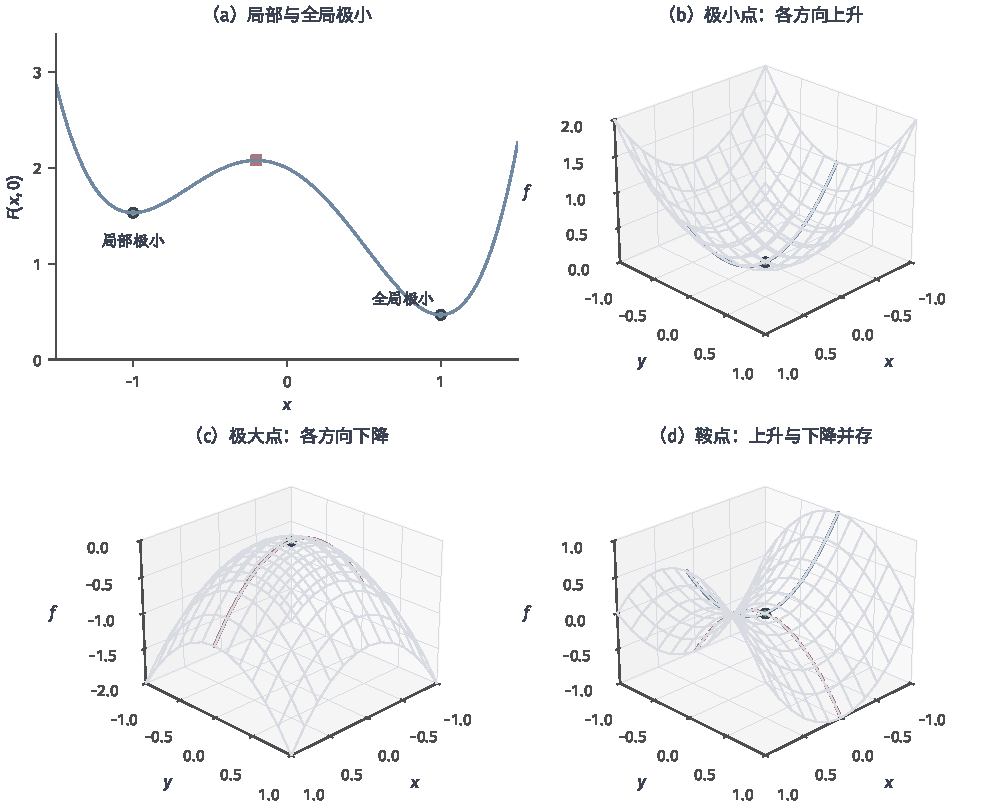
\includegraphics[width=159.059mm]{figures/05-neural-network-models/00-shared/matplotlib/training-stationary-points/figure.pdf}
  \caption{驻点与极值的构造示意。（a）为$F(x,y)=1+(x^2-1)^2+0.8(x^3/3-x)+y^2$的$y=0$截面。$(-1,0)$是非全局局部极小，$(1,0)$是全局极小，方点$(-0.2,0)$是完整曲面的鞍点。（b）$f=x^2+y^2$；（c）$f=-x^2-y^2$；（d）$f=x^2-y^2$。后三图绿色中心点均为驻点，蓝色实线表示上升切片，红色线表示下降切片。图示为解析函数，不是网络损失的实测图。}
  \label{fig:training-stationary-points}
\end{figure*}

训练为何会遇到这些形状，可以从最简单的两层线性模型看起。令标量预测为$uv$、目标为1，平方损失为
\begin{equation}
  \mathcal L(u,v)=\tfrac12(uv-1)^2,\qquad
  \nabla\mathcal L=(uv-1)(v,u)^{\top}\text{。}
  \label{eq:training-factorized-saddle}
\end{equation}
损失对预测$uv$是凸的，对两层参数$(u,v)$却不是。在$(0,0)$处，梯度为0、损失为$1/2$，Hessian的两个特征值为1和$-1$。沿$u=v$的小扰动降低损失，沿$u=-v$则提高损失；只沿任一坐标轴观察，损失还保持不变。两层参数的乘积已经形成鞍点，更多参数组合、非线性与样本叠加还会改变这份几何。输出损失的凸性因而需要和参数空间的性质分别判断。

\term{平坦区域}（flat region）指在所考察尺度内目标或梯度变化很小的区域，不必包含严格驻点。饱和激活、参数冗余或近似对称性都可能产生这类区域。在这种区域内，损失值说明离训练目标多远，梯度尺度和邻近更新则说明当前位置能提供多少推进信号。

梯度下降若精确到达零梯度驻点，就没有一阶更新；在其附近，梯度很小也会让推进缓慢。鞍点还有可下降方向，但小梯度未必明显指向它；非全局局部极小则需要离开当前邻域才能到达更低区域。高维鞍点及附近平台的研究将小梯度与可下降方向联系起来，为判断停滞提供了曲率依据\scite{dauphin2014saddle}

扰动在可下降方向上有分量时，可能将参数送离某些鞍点或平台；若每个样本在零参数处的梯度都为0，抽样也会继续给出0。参数置换和尺度对称还让同一个预测函数对应多个参数位置。驻点性质描述当前位置的目标形状，训练误差描述样本拟合，泛化风险则描述新数据预测。

\subsection{病态曲率}
\label{sec:training-curvature}

一个方向陡、另一个方向缓时，同一学习率需要同时照顾两种变化速度。即使目标只有一个全局极小点，也可能出现这种更新困难；分解参数化还会改变相应动力学（参考\BookEquationRef{eq:factorized-gradient-flow}{卷3《基础、理论与可信性》第8章“深度学习的可学习性”第8.4.4节“谱偏好与矩阵预测的泛化”}）。考虑教学目标
\begin{equation}
  q(\bm\theta)=\tfrac12(a\theta_1^2+b\theta_2^2),
  \qquad a\gg b>0\text{。}
  \label{eq:training-quadratic}
\end{equation}
两个方向分别以$a$和$b$的尺度变化。固定步长梯度下降在第一个方向的系数为$1-\eta a$，在第二个方向为$1-\eta b$。要让任意初始位置的两个方向都收缩，必须取$0<\eta<2/a$；这个步长在缓方向却只能带来很小的变化。

\term{病态曲率}（ill-conditioned curvature）描述不同方向的曲率尺度相差很大的情形。正定二次目标的\term{条件数}（condition number）为$\kappa=\lambda_{\max}(\bm H)/\lambda_{\min}(\bm H)$。在该模型中，最优固定步长$2/(a+b)$对应的最坏方向收缩因子为$(\kappa-1)/(\kappa+1)$，条件数大时接近1。若步长让陡方向的系数为负，参数会交替越过谷底，表现为振荡。

取$a=100,b=1,\eta=0.015$，陡方向每步乘以$-0.5$，缓方向每步乘以0.985。图~\ref{fig:training-curvature}左图显示这个稳定步长下的轨迹：左右振荡迅速缩小，轨迹落到谷底附近，但第80步仍未到达极小点。此时是收敛慢，继续迭代仍会趋向原点。

为了加快缓方向，若把步长增到临界值$\eta=2/a=0.02$，陡方向系数就变为$-1$。右图从上方观察同一谷地：$\theta_1^{(t)}=0.35(-1)^t$一直在两侧来回切换，$\theta_2^{(t)}=0.98^t$虽然逐渐减小，却不能带动陡方向的摆幅收缩。损失趋向$100\times0.35^2/2=6.125$，而最小值是0；这时增加迭代次数也无法收敛到原点。步长再大还会发散。两图共同显示了单一全局步长的矛盾：照顾陡方向时缓方向走得慢，试图加快缓方向又可能在陡方向越过头。动量利用历史方向缓解某些振荡，\term{预条件}（preconditioning）则通过矩阵或逐坐标尺度变换，让更新适应不同方向的变化速度。
\begin{figure*}[htbp]
  \centering
  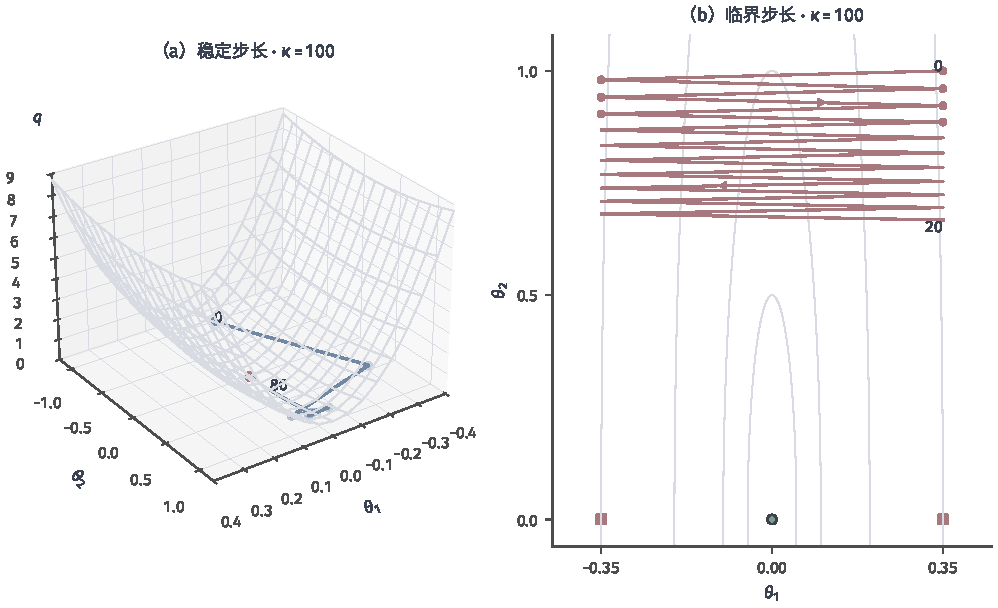
\includegraphics[width=159.059mm]{figures/05-neural-network-models/00-shared/matplotlib/training-curvature/figure.pdf}
  \caption{同一病态二次目标在两种步长下的轨迹，标题直接标出条件数$\kappa=a/b=100$，绿色点为极小点。（a）三维图采用稳定步长0.015，蓝色实心圆标出第0--8步，空心圆标出第80步；陡方向收缩快，谷底推进慢。（b）俯视投影采用临界步长0.02，深红线连接第0--20步，实心圆标出第0--6步，空心圆为第20步；灰线为等高线，竖虚线为谷底。左右摆幅保持0.35，损失趋向6.125而无法达到原点处的0。}
  \label{fig:training-curvature}
\end{figure*}
\FloatBarrier

重缩放同一函数的参数坐标，会改变Hessian特征值与梯度下降轨迹，归一化和重参数化因此也会影响优化。上面的条件数与收缩率针对正定二次目标；非凸区域还要处理零或负曲率。

\subsection{非精确梯度}
\label{sec:training-inexact-gradients}

完整经验梯度需要访问全部样本。小批量用抽到的样本估计这份梯度，估计的波动和系统偏差会以不同方式进入更新；随机梯度的结论也以抽样、步长和损失为条件（参考\BookSectionRef{sec:sgd-stability}{卷3《基础、理论与可信性》第7章“一般学习的可学习性”第7.4.3节“凸学习问题的随机梯度下降”}）。每步选$b$个样本组成索引多重集$B^{(t)}$（允许同一索引重复出现），计算
\begin{equation}
  \bm g^{(t)}=\frac1b\sum_{i\in B^{(t)}}
    \nabla_{\bm\theta}\ell(f_{\bm\theta^{(t-1)}}(\bm x_i),y_i)\text{。}
  \label{eq:training-minibatch-gradient}
\end{equation}
若在给定当前参数后独立、均匀、有放回抽样，条件期望等于完整经验梯度。独立抽样下，其协方差为单样本梯度协方差的$1/b$；无放回抽样还有有限总体修正。按顺序遍历一段相关视频，或在一个轮次内随机重排后逐批读取，并不满足这一条件独立模型。

\term{随机方差}（stochastic variance）描述梯度估计围绕期望的波动，\term{系统性偏差}（systematic bias）则是估计期望与目标梯度的差异。扩大独立批量降低抽样方差；截断时间反向传播删除历史路径、错误缩放改变目标贡献，则需要修正相应计算。量化、有限精度和近似算子还会引入数值误差，是否具有偏差取决于具体实现。

梯度累积可以把多个小批量的梯度合成为较大批量更新，但要求它们在同一参数位置计算，并按样本数或有效词元数正确加权。BatchNorm等依赖当前批量的操作、随机失活及不同长度掩码，会使“分批累积”与“一次大批量前向”具有不同计算图。批量还决定每轮包含多少次更新，因此更新步数、样本访问量与时间预算构成三种不同的比较条件。

\subsection{梯度传播与长期依赖}
\label{sec:training-gradient-propagation}

误差从输出传到早期表示，需要穿过沿途的局部导数。即使输出梯度与抽样估计准确，连乘仍可能使某些方向的信号衰减或放大。残差、门控、初始化与参数约束通过改变这些路径或因子参与训练。对于$L$层复合映射，记$\bm J_l=\partial\bm h^{(l)}/\partial\bm h^{(l-1)}$，若梯度按列向量表示，则
\begin{equation}
  \nabla_{\bm h^{(s)}}\ell
  =\bm J_{s+1}^{\top}\cdots\bm J_L^{\top}
    \nabla_{\bm h^{(L)}}\ell\text{。}
  \label{eq:training-jacobian-chain}
\end{equation}
沿某些方向反复缩小，会形成\term{梯度消失}（vanishing gradients）；反复放大，则可能形成\term{梯度爆炸}（exploding gradients）。算子范数给出上界$\lVert\nabla_{\bm h^{(s)}}\ell\rVert_2\leq\prod_{l>s}\lVert\bm J_l\rVert_2\,\lVert\nabla_{\bm h^{(L)}}\ell\rVert_2$。上界描述可能的最大放大；实际梯度沿哪些方向传播，还取决于奇异向量对齐和各支路的抵消。

循环网络沿时间重复使用状态映射，出现同类Jacobian矩阵连乘。饱和激活的小导数、权重尺度、网络深度和递推长度都会影响传播。裁剪处理已经算出的异常大值，接近0的历史信号则需要改变传播路径。前向状态怎样保存输入、后来的损失怎样影响早期参数，是同一计算图上的两个问题。

\section{优化方法}
\label{sec:training-optimizers}

一次参数更新需要决定往哪里走、走多远，以及当前梯度有多少可以信任。第\ref{sec:training-challenges}节的目标几何、病态曲率和非精确梯度，分别给这三个决定带来困难。方向、尺度与噪声分别对应不同的更新机制：
\begin{itemize}
  \item \textbf{下降方向。} 负的完整梯度给出欧氏坐标下的局部最陡下降方向，但弯曲谷地中沿这个方向反复更新可能绕路；小批量梯度还会偏离完整目标的方向。动量借助历史判断持续趋势，预条件和曲率方法利用方向间的耦合修正更新。小梯度区域的曲率与损失值再决定当前信号是否已经接近所求目标。
  \item \textbf{下降尺度。} 步长过小会让训练长时间停留在高损失区，过大又可能跨过谷底、持续振荡甚至发散。希望方法同时管理整体学习率和不同方向的相对尺度，在缓方向充分推进，在陡方向限制更新，并随训练阶段减小需要精细调整时的步幅。调度、逐坐标缩放、阻尼和步长搜索分别处理这些尺度选择。
  \item \textbf{噪声适应。} 小批量梯度会随样本改变，异常大值、稀疏访问和非平稳统计又会使历史参照失准。批量平均、历史平滑、遗忘机制与裁剪可以控制其中不同部分；过强平滑会滞后，过大步长会放大噪声，过快遗忘则难以识别趋势。截断计算和错误缩放产生的偏差则需要处理其来源。
\end{itemize}
方向与尺度需要一起判断。精确下降方向也可能因步长过大而提高损失，较小更新则可能只是停滞。更复杂的估计还会增加求解、通信和历史状态，达到同一训练目标的总时间与峰值存储将这些额外开销计入比较。非凸目标上的这些改进依赖相应条件；计算图内部已经消失的梯度，仍需在第\ref{sec:training-connections}节改善传播路径，泛化表现则由第\ref{chap:neural-network-generalization}章另行判断。

为了比较不同方法，可以把优化器看成一个带记忆的更新过程：接收当前位置的信息，读取历史状态，按规则计算参数增量，再保存下一步需要的状态。沿这个更新过程，可以检查四种信息：
\begin{itemize}
  \item \textbf{输入。} 基本方法接收当前参数与完整或抽样梯度；曲率方法还使用Hessian、输出Jacobian矩阵或Fisher相关信息，步长搜索还需评估候选位置的损失。输入的精度、抽样方式和获取成本，限定了方法能作出怎样的判断。
  \item \textbf{状态。} 无动量SGD不保存与参数同规模的历史缓冲；动量保存方向，AdaGrad与RMSProp保存平方梯度统计，Adam同时保存两种矩，L-BFGS保存有限组参数差与梯度差。状态还可能是分层矩阵、行列因子和调度进度，其大小与遗忘方式决定成本和适应速度。
  \item \textbf{方法。} 可直接沿梯度缩放，也可先平滑方向、按坐标调整尺度、求解耦合方向的线性系统，或提取符号、整形奇异值。裁剪、阻尼、偏差修正与学习率调度可以参与这个计算；近似方式决定保留哪些关系、舍弃哪些信息。
  \item \textbf{输出。} 对训练循环而言，输出是参数增量$\Delta\bm\theta^{(t)}$或等价的新参数，以及更新后的历史状态。增量的方向、长度、坐标比例和可行性显示前三项怎样进入实际更新；预条件和历史状态还会改变原始梯度上限对应的位移。
\end{itemize}

这四个维度描述同一个优化器，可以交叉组合。例如，SGD以当前梯度为输入、没有方向历史，方法是乘以学习率，输出$\Delta\bm\theta^{(t)}=-\eta_t\bm g^{(t)}$；Adam仍以当前梯度为主要输入，却用两种历史状态构造平滑方向与逐坐标尺度，因此输出的方向和长度都可能不同。共同的梯度输入经过不同状态与计算，产生不同增量；平方梯度统计记录历史幅度，Hessian记录当前位置的曲率。

下面沿这个共同过程展开：基本更新、调度和裁剪建立基准；动量与自适应方法增加历史状态；牛顿、拟牛顿、GGN和自然梯度使用更强的几何信息或估计；K-FAC、Shampoo和Muon利用层或矩阵结构改变计算与输出。这些方法各自保留不同几何信息，其实际增量和成本由具体输入、状态及计算规则确定。

在共同记号下，可将许多更新写为$\bm\theta^{(t)}=\bm\theta^{(t-1)}-\eta_t\bm P^{(t)}\bm d^{(t)}$。$\bm d^{(t)}$由当前梯度及历史信息构成，$\bm P^{(t)}$为尺度变换或预条件矩阵，$\eta_t$为全局学习率。这个分解帮助辨认方法改变了方向、逐坐标尺度，还是随训练进程变化的整体步长；有些实现直接求方向或计算矩阵作用，无需显式保存$\bm P^{(t)}$。

\subsection{梯度下降与随机梯度下降}
\label{sec:training-gradient-schedules}

基本更新将当前完整梯度或抽样梯度按步长缩放，再从参数中减去（参考\BookSectionRef{sec:opt-gradient-descent}{卷1《数学准备：计算、分析与几何》第4章“最优化”第4.2.1.1节“基于梯度下降的求解”}和\BookSectionRef{sec:opt-stochastic-gradient-stability}{卷1《数学准备：计算、分析与几何》第4章“最优化”第4.5.4节“基于近似更新的求解”}）。对网络训练目标$\mathcal L$使用完整梯度或小批量梯度$\bm g^{(t)}$，更新为
\begin{equation}
  \bm\theta^{(t)}=\bm\theta^{(t-1)}-\eta_t\bm g^{(t)}\text{。}
  \label{eq:training-sgd}
\end{equation}
在更新线段内目标梯度为$L_s$-Lipschitz时，下降引理给出完整梯度在$0<\eta<2/L_s$下的下降界；梯度非零时严格下降，驻点处保持不动。ReLU切换点改变光滑条件，抽样噪声改变所用方向；相应更新按各自条件分析。

小批量SGD的每一步既受到当前下降方向影响，也受到抽样噪声影响。
在本步所有可能的更新线段上满足同一光滑条件时，若$\bm g=\nabla\mathcal L+\bm\xi$，给定当前参数时
$\mathbb E[\bm\xi\mid\bm\theta]=\bm0$且$\mathbb E[\lVert\bm\xi\rVert_2^2\mid\bm\theta]<\infty$，
代入光滑性上界并取条件期望，得到
\begin{equation}
  \begin{aligned}
  \mathbb E[\mathcal L(\bm\theta-\eta\bm g)\mid\bm\theta]
  \leq{}&\mathcal L(\bm\theta)
    -\eta(1-L_s\eta/2)\lVert\nabla\mathcal L\rVert_2^2\\
    &+\tfrac12L_s\eta^2\mathbb E[\lVert\bm\xi\rVert_2^2\mid\bm\theta]\text{。}
  \end{aligned}
  \label{eq:training-stochastic-descent}
\end{equation}
噪声项随$\eta^2$增长；当真实梯度很小时，它可能抵消这一步的预期下降。减小步长或扩大独立批量可以改变这项，但也改变推进速度和计算量。在梯度较小的后期，这份波动就可能成为更新的主要成分。

SGD的优势是更新简单、额外状态少，小批量避免每一步遍历全部数据；完整梯度则消除了抽样方差，更便于判断局部下降。代价分别是随机波动和较高的数据访问成本，而且两者都用同一全局步长面对不同方向的曲率。一次基本更新不额外维护与$p$同规模的历史状态。前向、反向和数据访问共同决定每步时间，与所需步数一起构成完整训练成本。

\subsection{学习率调度}
\label{sec:training-schedules}

式\eqref{eq:training-stochastic-descent}中，推进项随步长增长，噪声项却随步长平方增长；训练早期与接近解时未必需要相同尺度。调度通过改变整体步长处理这一阶段差异。\term{学习率调度}（learning rate scheduling）按训练进程改变$\eta_t$。固定学习率维持同一更新尺度；分段衰减在预定里程碑乘以小于1的系数；指数衰减可以写为$\eta_t=\eta_0\gamma^t$，$0<\gamma<1$。若固定总训练长度，余弦调度可将学习率从$\eta_{\max}$平滑降到$\eta_{\min}$：
\begin{equation}
  \eta_t=\eta_{\min}+\frac{\eta_{\max}-\eta_{\min}}2
  \left[1+\cos\left(\frac{\pi(t-t_w)}{T-t_w}\right)\right],
  \quad t_w\leq t\leq T\text{。}
  \label{eq:training-cosine-schedule}
\end{equation}
这里$T$为总更新次数，$t_w$为预热结束步，总步数须大于预热步数。\term{预热}（warmup）在训练早期逐步增加学习率，有预热时，例如前$t_w$步取$\eta_t=\eta_{\max}t/t_w$，让初始参数和优化器统计量在较小更新下开始适应。周期性调度则反复升降，带重启的余弦调度是其中一种形式\scite{loshchilov2017sgdr}

调度以很小的额外成本区分早期推进与后期精细调整，预热还能限制尚未稳定的初始更新。但衰减过早可能在高损失区停滞，过晚可能延长解附近的波动；预定总长度也未必适应中途改变的预算。调度可以按更新步、样本访问量或训练轮次计时，这些单位在批量改变时不再等价。全局$\eta_t$决定整步的基础尺度，后面的自适应方法再调整相对尺度。预热与衰减只改变整步尺度，所用梯度和候选目标仍需满足相应训练条件。

例如，计划训练1000步，前100步线性预热，随后用式\eqref{eq:training-cosine-schedule}衰减。第100步恰好到达$\eta_{\max}$，第550步为两端学习率的平均，第1000步到达$\eta_{\min}$。若恢复第550步的参数却从调度起点重新计时，后续轨迹就与原计划不同。调度状态因此属于恢复训练所需的信息。

\subsection{梯度裁剪}
\label{sec:training-gradient-modification}

第\ref{sec:training-gradient-propagation}节中的连乘可能产生偶发的大梯度，数值误差也可能放大更新，使参数离开当前有用区域。\term{梯度裁剪}（gradient clipping，也称梯度截断）在优化器使用梯度之前限制这份信号。逐元素裁剪令$\tilde g_j=\max(-c,\min(c,g_j))$，$c>0$，它改变部分坐标的相对比例；整体范数裁剪则为
\begin{equation}
  \tilde{\bm g}=\bm g\min\left(1,\frac{c}{\lVert\bm g\rVert_2}\right)\text{，}
  \label{eq:training-norm-clipping}
\end{equation}
零梯度直接保留。整体裁剪在非零时保持方向，但会引入与梯度大小有关的偏差。裁剪后的梯度还可能被动量或自适应尺度放大，所以梯度范数上限不等于最终参数步长上限。

取$\bm g=(3,4)^{\top}$，范数为5，整体上限$c=2$给出$(1.2,1.6)^{\top}$；逐元素上限2则给出$(2,2)^{\top}$，方向已改变。两种裁剪都控制极端更新，小于上限的信号保持原样。若几乎每步都被大幅裁剪，损失缩放、初始化或状态递推可能持续产生过大梯度，需要定位这份来源。

\subsection{动量法}
\label{sec:training-momentum}

陡方向的梯度可能来回变号，缓方向却持续指向谷底。把历史与当前方向累积起来，同向部分得到保留，交替部分可以抵消（参考\BookSectionRef{sec:opt-curvature-acceleration}{卷1《数学准备：计算、分析与几何》第4章“最优化”第4.2.1.2节“基于动量与加速的求解”}）。采用未归一化的累积约定，从零缓冲开始，令
\begin{equation}
  \bm m^{(t)}=\beta\bm m^{(t-1)}+\bm g^{(t)},\qquad
  \bm\theta^{(t)}=\bm\theta^{(t-1)}-\eta_t\bm m^{(t)},
  \quad\beta\in[0,1)\text{。}
  \label{eq:training-momentum}
\end{equation}
交替的梯度会部分抵消，持续同向的梯度会积累。如果$\bm g^{(t)}$近似恒定，累积量趋向$\bm g/(1-\beta)$，因此调整$\beta$也改变有效更新尺度。另一约定在梯度前乘$1-\beta$；比较实现时要同时对应学习率。

精确二次目标中的误差递推可以给出谱速率，网络训练中的曲率和抽样梯度则随位置变化。较大的$\beta$延长历史记忆，同时放大未归一化缓冲的有效尺度；系数选择据实际目标与更新评价。

动量只增加一个$p$维缓冲，但也使更新具有惯性。梯度突然换方向时，旧方向不会立即消失；较大的$\beta$提供更长历史，也可能让响应迟缓。它对噪声的平滑和对有效步长的放大应一起考虑。

\subsection{Nesterov加速梯度}
\label{sec:training-nesterov}

动量保存旧方向，也可能在接近谷底时继续推动参数。Nesterov方法让梯度读取历史方向预计到达的位置，以修正这种惯性。\term{Nesterov加速梯度}（Nesterov accelerated gradient, NAG）在历史方向指向的前瞻位置计算梯度，而不是只对当前位置的梯度做累积。对式\eqref{eq:training-momentum}的约定，可写为
\begin{align}
  \bar{\bm\theta}^{(t)}&=\bm\theta^{(t-1)}-\eta_t\beta\bm m^{(t-1)},\\
  \bm m^{(t)}&=\beta\bm m^{(t-1)}+
       \nabla\mathcal L(\bar{\bm\theta}^{(t)}),\qquad
  \bm\theta^{(t)}=\bm\theta^{(t-1)}-\eta_t\bm m^{(t)}\text{。}
  \label{eq:training-nesterov}
\end{align}
前瞻梯度提供对惯性方向的修正。深度学习实现常采用等价变换或固定动量的变体；经典加速率分析以凸目标和相应系数为条件，非凸抽样更新还需另外分析。

以一维$q(\theta)=a\theta^2/2$为例，普通动量读取$a\theta$，前瞻形式读取$a(\theta-\eta\beta m)$。若惯性正将参数推向谷底，前瞻梯度已看到较低位置，从而减少继续沿旧方向推进的量；若已越过谷底，则可能更早得到相反方向的修正。这组一维计算展示前瞻怎样修正方向，实际下降还取决于曲率与步长。

式\eqref{eq:training-nesterov}直接展示“到前瞻位置求导”的定义。实际实现也可把参数位置作等价重写，以避免额外前向计算；变动学习率或动量时，等价关系需要重新对应。求导位置、缓冲约定和最终增量共同确定不同实现是否对应同一更新。

前瞻的优势是让惯性修正在本步方向形成前发生，在相应凸条件下可得到加速结论。它仍保留动量的历史滞后，也会受到前瞻位置梯度噪声的影响；非凸网络中前瞻点可能落入与当前位置不同的局部形状。前瞻因此改变方向的形成方式，步长与动量继续决定该方向产生的位移。

\subsection{AdaGrad}
\label{sec:training-adaptive}

有些参数经常收到大梯度，有些只在少数样本出现时更新，同一全局步长无法分别照顾两者。\term{自适应学习率}（adaptive learning rate）用历史梯度统计量为不同坐标设置相对尺度。逐坐标统计比完整矩阵便宜，但不完整描述第\ref{sec:training-curvature}节中的方向耦合；历史统计记录观测梯度的大小与频率，局部曲率则还包含方向之间的耦合。

AdaGrad累计逐坐标平方梯度。令$\bm v^{(0)}=\bm0$，其常见对角形式为
\begin{equation}
  \bm v^{(t)}=\bm v^{(t-1)}+\bm g^{(t)}\odot\bm g^{(t)},\qquad
  \bm\theta^{(t)}=\bm\theta^{(t-1)}-
  \eta\frac{\bm g^{(t)}}{\sqrt{\bm v^{(t)}}+\epsilon}\text{。}
  \label{eq:training-adagrad}
\end{equation}
$\odot$为逐元素乘法，$\epsilon>0$防止分母为0。反复收到大梯度的坐标逐渐减小更新尺度，较少更新的坐标则保留较大相对尺度。累积量不减小，长期训练中步长可能变得过小\scite{duchi2011adagrad}

若某个坐标每步收到相同的非零梯度$g$，忽略$\epsilon$时，第$t$步的更新幅度为$\eta/\sqrt t$；梯度的绝对尺度被平方累积抵消。一个很少出现的特征则只在出现时增加该坐标累积量，因此按访问次数减小步长。按访问次数累积的尺度使稀疏坐标获得不同步幅；其训练效果还与目标、数据和所选学习率有关。

AdaGrad增加一个$p$维累积量，每步的逐元素处理为$O(p)$。累计统计无法主动忘记训练早期的大梯度：目标分布或训练阶段改变后，早期尺度仍会限制当前更新。RMSProp接下来用有限记忆缓解这一点。

\subsection{RMSProp}
\label{sec:training-rmsprop}

AdaGrad的累计历史不遗忘，早期大梯度可能长期压低后续步长。若训练阶段的尺度改变，指数平均可以让近期梯度重新决定分母。RMSProp改用近期平方梯度的指数移动平均：$\bm v^{(t)}=\rho\bm v^{(t-1)}+(1-\rho)\bm g^{(t)}\odot\bm g^{(t)}$，再用式\eqref{eq:training-adagrad}中的分母更新，$\rho\in[0,1)$。旧梯度影响衰减，因此相对尺度可以随着训练阶段改变。其平方平均、开方和稳定项的位置应以具体实现为准\scite{hinton2012rmsprop}

为明确它与AdaGrad的不同，把更新完整写为
\begin{equation}
  \begin{aligned}
  \bm v^{(t)}&=\rho\bm v^{(t-1)}+(1-\rho)\bm g^{(t)}\odot\bm g^{(t)},\\
  \bm\theta^{(t)}&=\bm\theta^{(t-1)}-
    \eta_t\bm g^{(t)}/(\sqrt{\bm v^{(t)}}+\epsilon)\text{。}
  \end{aligned}
  \label{eq:training-rmsprop}
\end{equation}
过去第$s$步平方梯度在第$t$步的权重为$(1-\rho)\rho^{t-s}$。较大的$\rho$使尺度变化更平缓，却更慢适应新梯度；较小的$\rho$响应更快，也增加分母波动。零初值下的恒定梯度给出$v^{(t)}=(1-\rho^t)g^2$，因此早期分母尚未达到稳态，初始更新可能比稳态更大。

基本RMSProp使用一个$p$维二阶矩状态，可另外组合动量。它观察的是当前坐标的历史平方梯度，对坐标旋转通常不具有不变性，也不利用坐标之间的耦合。全局学习率仍控制整体步幅，坐标间尚未记录的耦合则可能继续影响曲率适配。

\subsection{AdaDelta}
\label{sec:training-adadelta}

只根据平方梯度设置分母，仍需选择参数实际移动的尺度。AdaDelta把近期更新也纳入统计，用更新与梯度的两类均方根之比调节幅度，减少对单一固定全局尺度的依赖。设$\bm v^{(t)}$为上述平方梯度平均，$\bm r^{(t)}$为平方更新平均，则原始基本形式为
\begin{align}
  \Delta\bm\theta^{(t)}&=-\frac{\sqrt{\bm r^{(t-1)}+\epsilon}}
                               {\sqrt{\bm v^{(t)}+\epsilon}}
                                \odot\bm g^{(t)},\\
  \bm r^{(t)}&=\rho\bm r^{(t-1)}+(1-\rho)
      \Delta\bm\theta^{(t)}\odot\Delta\bm\theta^{(t)},\\
  \bm\theta^{(t)}&=\bm\theta^{(t-1)}+\Delta\bm\theta^{(t)}\text{。}
  \label{eq:training-adadelta}
\end{align}
分子使用前一步统计量，避免与本步更新形成循环定义。这个基本形式没有独立的全局学习率，但仍需选择$\rho$、稳定项和初值；有些实现再乘全局系数，相应尺度也进入实际增量\scite{zeiler2012adadelta}

如果某个坐标近期更新很小，分子会减小该坐标的更新；梯度尺度上升时，分母则抑制幅度。分子与分母共同把近期参数变化和近期梯度联系起来，这是它区别于仅累计梯度平方的方法之处。两个状态均按坐标保存，额外存储为$O(p)$，但常数是两组统计量。

稳定项同时承担零初值启动的作用。如果$r^{(0)}=0$且完全去掉$\epsilon$，第一步分子就为0；尚未发生的更新因而没有为分子提供初始尺度。实际$\epsilon$的数值与单位、$\rho$及全局缩放约定都会影响轨迹。

\subsection{Adam与AMSGrad}
\label{sec:training-adam}

抽样噪声影响方向，坐标尺度差异影响幅度；单独的动量或平方统计各处理一部分。Adam同时维护梯度的一阶矩和非中心化二阶矩，前者给平滑方向，后者给逐坐标尺度，以较低的逐元素计算成本组合两种处理。AMSGrad进一步管理分母随时间变化的问题。以零初值定义
\begin{align}
  \bm m^{(t)}&=\beta_1\bm m^{(t-1)}+(1-\beta_1)\bm g^{(t)},\\
  \bm v^{(t)}&=\beta_2\bm v^{(t-1)}+(1-\beta_2)
                 \bm g^{(t)}\odot\bm g^{(t)},\\
  \hat{\bm m}^{(t)}&=\frac{\bm m^{(t)}}{1-\beta_1^t},\qquad
  \hat{\bm v}^{(t)}=\frac{\bm v^{(t)}}{1-\beta_2^t},\\
  \bm\theta^{(t)}&=\bm\theta^{(t-1)}-
    \eta_t\frac{\hat{\bm m}^{(t)}}{\sqrt{\hat{\bm v}^{(t)}}+\epsilon}\text{。}
  \label{eq:training-adam}
\end{align}
$\beta_1,\beta_2\in[0,1)$为平滑系数。分母中的修正因子来自零初值：把$\bm m^{(0)}=\bm0$代入递推，假设第1至$t$步梯度具有相同的有限均值$\mathbb E[\bm g^{(s)}]=\bm\mu$，就有
\begin{equation}
  \begin{aligned}
    \bm m^{(t)}&=(1-\beta_1)\sum_{s=1}^{t}\beta_1^{t-s}\bm g^{(s)},\\
    \mathbb E[\bm m^{(t)}]
      &=(1-\beta_1)\sum_{s=1}^{t}\beta_1^{t-s}\bm\mu
        =(1-\beta_1^t)\bm\mu\text{。}
  \end{aligned}
  \label{eq:training-adam-bias-correction}
\end{equation}
第二行只用期望的线性性质与等比求和，不要求各步梯度相互独立。有限步的权重和是$1-\beta_1^t$，尚未达到1；除以它，便在上述同均值假设下得到$\mathbb E[\hat{\bm m}^{(t)}]=\bm\mu$。同理，若各步的逐坐标非中心二阶矩均为$\bm\nu=\mathbb E[\bm g^{(s)}\odot\bm g^{(s)}]$且有限，零初值$\bm v^{(0)}=\bm0$给出$\mathbb E[\bm v^{(t)}]=(1-\beta_2^t)\bm\nu$。这里没有减去梯度均值，$\bm\nu$不是梯度方差。偏差修正消除的是零初始化的权重缺口；实际梯度统计随参数变化，抽样偏差由取样方式决定，当前矩与历史平均的差别则随参数变化保留\scite{kingma2015adam}

这里的二阶矩是$g_j^2$的平均，Hessian是损失对参数的二阶导数。前者即使在负曲率区域也非负，且包含梯度均值和噪声方差；后者可以有负特征值。Adam属于用一阶梯度统计构造更新的方法。全局学习率和调度继续决定整步位移，训练速度与泛化风险再在共同任务和预算下比较。

Adam的第一次更新很有辨识度：零初值下，偏差修正后$\hat m^{(1)}=g^{(1)}$、$\hat v^{(1)}=(g^{(1)})^2$，所以忽略$\epsilon$时，非零坐标按$-\eta_1\operatorname{sign}(g^{(1)})$移动。后续步由不断改变的历史方向和尺度共同决定，更新比例随之变化。两组$p$维状态增加存储，恢复训练时也必须恢复它们。

Adam的指数平均可能降低分母，使某个坐标的有效步长重新增大。\term{AMSGrad}用历史最大二阶矩阻止这种下降。省略初始化偏差修正时，可写为
\begin{equation}
  \bar{\bm v}^{(t)}=\max(\bar{\bm v}^{(t-1)},\bm v^{(t)}),\qquad
  \bm\theta^{(t)}=\bm\theta^{(t-1)}-
    \eta_t\bm m^{(t)}/(\sqrt{\bar{\bm v}^{(t)}}+\epsilon)\text{，}
  \label{eq:training-amsgrad}
\end{equation}
最大值逐元素计算，$\bar{\bm v}^{(0)}=\bm0$。加入偏差修正的实现还需对应其具体约定。AMSGrad针对Adam的某些收敛问题提出，但其收敛分析针对相应目标与更新条件；历史最大值限制后期分母下降，同时减少对较小梯度尺度的适应\scite{reddi2018amsgrad}

图~\ref{fig:training-optimizer-trajectories}把SGD、动量和Adam放到同一个病态二次目标上逐步计算。SGD在陡方向反复越过谷底，缓方向只按固定比例缩小；动量利用历史方向加快沿谷底推进，但仍带有惯性振荡；Adam在这个轴对齐例子中按坐标缩放，前几步几乎沿对角线接近原点。三条轨迹对应图中各自给定的超参数，显示同一目标中方向与尺度怎样进入更新。
\begin{figure}[htbp]
  \centering
  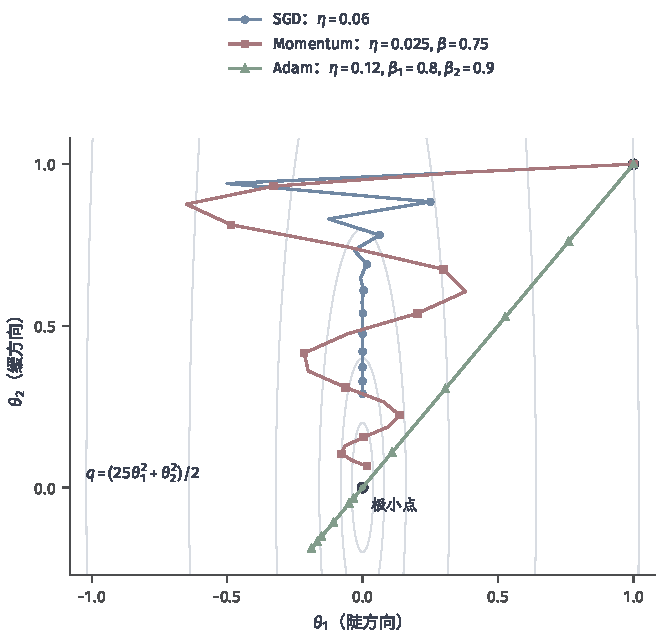
\includegraphics[width=105.412mm]{figures/05-neural-network-models/00-shared/matplotlib/training-optimizer-trajectories/figure.pdf}
  \caption{SGD、动量与Adam在同一病态二次目标上的前20步。目标为$q(\bm\theta)=(25\theta_1^2+\theta_2^2)/2$，条件数$\kappa=25$，三者均从$(1,1)^\top$出发并使用完整梯度；灰线为等高线，绿色点为唯一极小点。轨迹由正文定义的递推式直接计算，图例列出步长和矩系数。图示比较固定了目标与起点，超参数改变后速度与振荡也会改变；一般非凸抽样训练需相应评价。}
  \label{fig:training-optimizer-trajectories}
\end{figure}

AdamW将权重衰减与矩统计分开，公式及其与L2惩罚的区别见第\ref{sec:generalization-weight-decay}节。优化方向、步长统计与参数收缩是可以分别选择的三个设计对象。

\subsection{Adafactor与低存储二阶矩估计}
\label{sec:training-adafactor}

逐坐标尺度处理虽然便宜于完整曲率矩阵，在大模型中保存一张与参数同大的统计表仍可能昂贵。Adafactor通过保留行列边际，在历史存储与细节尺度之间取舍。\term{Adafactor}利用矩阵的行、列统计近似逐元素二阶矩，并可省去完整动量状态。被压缩的是逐元素平方梯度表，重构后仍按元素给出分母；曲率矩阵和左右预条件保留的是其他方向关系。

设矩阵参数为$\bm W\in\mathbb R^{m\times d}$，梯度为$\bm D^{(t)}$，取$A_{i,j}^{(t)}=(D_{i,j}^{(t)})^2+\epsilon_1$，$\epsilon_1>0$。令$r_i^{(t)}$和$c_j^{(t)}$分别为行均值与列均值的指数平均，一个简化形式为
\begin{align}
  r_i^{(t)}&=\beta_t r_i^{(t-1)}+(1-\beta_t)\frac1d\sum_j A_{i,j}^{(t)},\\
  c_j^{(t)}&=\beta_t c_j^{(t-1)}+(1-\beta_t)\frac1m\sum_i A_{i,j}^{(t)},\\
  \hat V_{i,j}^{(t)}&=\frac{r_i^{(t)}c_j^{(t)}}{m^{-1}\sum_k r_k^{(t)}}\text{。}
  \label{eq:training-adafactor-factorization}
\end{align}
两组均值从0以同一$\beta_t\in[0,1)$更新，其整体均值一致。重构表保留行、列边际，却不能保存任意单元素变化；某个格子的独特统计会被这种秩一结构近似。

得到$\bm U=\bm D/\sqrt{\hat{\bm V}}$后，原始方法还裁剪更新的均方根，并按参数尺度设置相对步长。记$\operatorname{rms}(\bm A)=\sqrt{(md)^{-1}\sum_{i,j}A_{i,j}^2}$，可以写为
\begin{equation}
  \bm\Delta=-\rho_t\max(\epsilon_2,\operatorname{rms}(\bm W))
    \frac{\bm U}{\max(1,\operatorname{rms}(\bm U)/c)}\text{，}
  \label{eq:training-adafactor-update}
\end{equation}
其中$\rho_t$为相对步长，$c>0$为更新上限，$\epsilon_2>0$控制近零参数的尺度。这里裁剪的是预条件后的更新，不同于前面裁剪原始梯度。统计衰减、相对步长与可选动量均需按具体实现指定\scite{shazeer2018adafactor}

不使用完整动量时，这个矩阵块的历史状态从$O(md)$降为$O(m+d)$，但梯度与临时更新仍有$md$个元素，整次训练还需把这些当前量与激活计入存储，$m+d$只描述该块的历史统计。向量参数通常不能按同样方式分解，仍需逐元素统计。

\subsection{Lion与符号动量更新}
\label{sec:training-lion}

历史方向的作用未必要求同时保存平方统计。Lion尝试只保留动量，以符号方向换取较少状态；代价是放弃梯度混合量的绝对幅度。\term{Lion}保留一组动量，用历史与当前梯度的混合决定各坐标的符号。取零初值，一个带解耦衰减的基本形式为
\begin{align}
  \bm z^{(t)}&=\beta_1\bm m^{(t-1)}+(1-\beta_1)\bm g^{(t)},\\
  \bm\theta^{(t)}&=(1-\eta_t\lambda)\bm\theta^{(t-1)}
      -\eta_t\operatorname{sign}(\bm z^{(t)}),\\
  \bm m^{(t)}&=\beta_2\bm m^{(t-1)}+(1-\beta_2)\bm g^{(t)}\text{。}
  \label{eq:training-lion}
\end{align}
两种平滑系数分别控制本步方向和留给后续的状态，均在$[0,1)$内，$\lambda\geq0$为衰减系数。更新使用旧动量，随后再保存新动量；把次序交换会改变算法\scite{chen2023lion}

符号操作让非零坐标的基础更新幅度相同，放弃了混合梯度的绝对大小。如果有$q$个非零符号，未计衰减时的更新范数就是$\eta_t\sqrt q$，这说明与Adam相同的学习率数值未必对应相同总步长。它增加一组$p$维状态，所存历史较少，符号方向则已舍去了混合量的绝对幅度。

\subsection{牛顿法、阻尼与步长控制}
\label{sec:training-second-order}

第\ref{sec:training-curvature}节中的主曲率方向未必与坐标轴对齐，逐坐标缩放可能留下明显的方向差异。
局部二次模型用曲率调整不同方向，得到耦合坐标的更新（参考\BookSectionRef{sec:opt-newton-gauss-newton}{卷1《数学准备：计算、分析与几何》第4章“最优化”第4.2.2.1节“基于牛顿与Gauss–Newton更新的求解”}）。使用当前训练Hessian $\bm H$与梯度$\bm g$，解阻尼系统$(\bm H+\lambda\bm I)\bm\Delta=-\bm g$，再选择步长。可逆性保证该系统有唯一解，正定性进一步使解成为二次模型的最小点；无阻尼的单位牛顿步在最优点附近Hessian正定且Lipschitz连续、初始点足够近时，可得到局部二次收敛。

\term{阻尼}（damping）用$\bm H+\lambda\bm I$调整曲率，$\lambda>0$足够大时可使其正定。\term{线搜索}（line search）在已有方向上试验多个步长，用实际目标检查下降；\term{信赖域}（trust region）则限制$\lVert\bm\Delta\rVert_2\leq r$，只在局部模型可信的范围内寻找更新，并依据预测下降与实际下降的吻合程度调节$r$。三种思路分别控制曲率、沿方向的距离和模型使用范围，可以组合。

曲率修正的优势是直接处理耦合与尺度差异，在光滑正定等局部条件下可以得到更快的局部收敛速率。代价是曲率计算和线性求解：显式矩阵需$O(p^2)$存储，一般稠密求解约为$O(p^3)$。局部模型不准确、Hessian接近奇异或小批量估计波动时，方向可能被过度放大；阻尼改善稳定性，也会削弱曲率修正。负曲率还应区别于数值错误，强行使矩阵正定会舍去这一逃离鞍点的信息。

\subsection{BFGS与L-BFGS}
\label{sec:training-quasi-newton}

相邻参数与梯度的变化可以估计曲率，省去直接计算完整Hessian（参考\BookSectionRef{sec:opt-quasi-newton}{卷1《数学准备：计算、分析与几何》第4章“最优化”第4.2.2.2节“基于拟牛顿更新的求解”}）。令$\bm s^{(t)}=\bm\theta^{(t)}-\bm\theta^{(t-1)}$、
$\bm y^{(t)}=\nabla\mathcal L(\bm\theta^{(t)})-\nabla\mathcal L(\bm\theta^{(t-1)})$。
拟牛顿更新可以用$\bm B$近似Hessian；本节用$\bm C$近似其逆，割线关系为$\bm C\bm y=\bm s$。两个矩阵分别描述曲率与逆曲率，构造更新时使用对应的逆作用。
正定初始近似及$\bm y^\top\bm s>0$仍是保持正定性的条件；
L-BFGS仅保存最近$k$组变化，减少大网络的历史存储。

小批量噪声可能让梯度差主要反映样本变化，而非参数变化，导致曲率估计失真。拟牛顿方法因此需要关注梯度差的数据一致性、批量和阻尼。完整矩阵的存储和线性求解仍是大网络使用二阶信息的主要约束\scite{bottou2018optimization}

L-BFGS用两轮递推从这些历史对计算逆曲率对梯度的作用，无需恢复完整矩阵。
对$p$个网络参数，$k$组历史的存储与方向计算均为$O(kp)$；
线搜索还会增加目标和梯度评估。训练循环必须让这些评估使用一致的数据与随机状态，
否则梯度差可能主要来自批量或Dropout变化，失去近似同一曲率的含义。

\subsection{广义Gauss--Newton方法}
\label{sec:training-generalized-curvature}

第\ref{sec:training-stationary-points}节说明了非凸Hessian可以包含负方向，直接求解未必得到下降步。GGN舍去网络输出非线性带来的一部分曲率，保留输出损失中更易控制的部分。令单样本网络输出为$\bm z_i=f_{\bm\theta}(\bm x_i)\in\mathbb R^c$，输出Jacobian矩阵为$\bm J_i\in\mathbb R^{c\times p}$，单样本损失为$\ell_i=\ell(\bm z_i,y_i)$。复合损失的Hessian可以分为
\begin{equation}
  \begin{aligned}
  \bm H=\frac1n\sum_i\bigg[
    &\bm J_i^{\top}\nabla_{\bm z_i}^2\ell_i\bm J_i\\
    &+\sum_{k=1}^c\frac{\partial\ell_i}{\partial z_{i,k}}
         \nabla_{\bm\theta}^2z_{i,k}\bigg]\text{。}
  \end{aligned}
  \label{eq:training-hessian-decomposition}
\end{equation}
第一项来自损失对输出的曲率，第二项来自网络输出对参数的非线性。\term{广义Gauss--Newton矩阵}（generalized Gauss--Newton matrix, GGN）只保留第一项，记为$\bm G$。若损失对输出凸，$\bm G$半正定；加阻尼后可用于构造下降方向，但它省略了真实Hessian的部分信息。

平方损失$\ell_i=\lVert\bm z_i-\bm y_i\rVert_2^2/2$对输出的Hessian是单位矩阵，于是$\bm G=n^{-1}\sum_i\bm J_i^{\top}\bm J_i$。输出对参数线性时，分解中的第二项为0，GGN等于真实Hessian；非线性网络中若残差接近0，第二项可能较小，但必须检查输出二阶导数与残差的乘积，这一乘积的大小决定所省略的曲率。

在当前点，把输出局部近似为$\bm z_i+\bm J_i\bm\Delta$，再保留损失的输出曲率，就能得到这种二次模型。它放弃部分非凸曲率，换来更容易控制的半正定矩阵；阻尼决定对低曲率方向放大多少，而求解精度决定是否接近该模型的最优更新。

\subsection{自然梯度与Fisher度量}
\label{sec:training-natural-gradient}

网络若定义条件概率$p_{\bm\theta}(y\mid\bm x)$，可以用相邻预测分布的变化衡量参数位移（参考\BookSectionRef{sec:information-natural-gradient-update}{卷2《数学准备：概率、因果与决策》第2章“概率分布”第2.6.2节“基于分布几何的参数更新”}）。固定输入评价分布$P_X$，本节的模型Fisher为
\begin{equation}
  \bm F=\mathbb E_{\bm x}\mathbb E_{y\sim p_{\bm\theta}(\cdot\mid\bm x)}
    [\bm a\bm a^{\top}],\qquad
  \bm a=\nabla_{\bm\theta}\log p_{\bm\theta}(y\mid\bm x)\text{。}
  \label{eq:training-fisher}
\end{equation}
在参数无关的共同支持、对数概率的参数梯度平方可积且可交换所需微分与积分等规则性条件下，邻近参数的平均KL二阶项为
$\bm\Delta^\top\bm F\bm\Delta/2$。
网络可能存在冗余参数，使$\bm F$奇异；实际计算常解
$(\bm F+\lambda\bm I)\bm\Delta=-\bm g$，其中$\lambda>0$为阻尼。
阻尼提供可求解的正则化方向，实际方向随阻尼和矩阵近似改变，相应重参数化不变性也会受到影响\scite{martens2020natural}

对负对数似然、以自然参数表示的指数族输出，合适定义下的GGN与模型Fisher可以相等。用训练标签的梯度外积直接平均得到的\term{经验Fisher}（empirical Fisher）却通常不同，因为标签来自数据，而非当前模型分布。Hessian、GGN、模型Fisher和经验Fisher描述的对象不同，只有给定输出模型与期望口径后才能讨论等价关系。

使用这些矩阵也不必显式生成全部$p^2$个元素。对向量$\bm v$，可以计算$\bm J_i\bm v$，再经输出损失曲率和$\bm J_i^{\top}$回传，得到$\bm G\bm v$；Hessian--向量乘积也可由自动微分实现。对正定的阻尼系统，用共轭梯度等迭代方法近似求解。每次迭代增加计算，停止容差、数据批量和矩阵近似共同决定更新质量。

\subsection{K-FAC}
\label{sec:training-structured-preconditioning}

若希望利用层内方向关系，又无法保存全部参数间的矩阵，网络层的输入与输出维度便提供了可利用的分解结构。K-FAC把这一结构用于Fisher近似，降低自然梯度的矩阵处理成本。完整矩阵同时保存所有参数间关系，代价随$p^2$增长。结构化方法只保存一部分：对角近似保留逐坐标尺度，分块近似保留块内关系，低秩近似保留少数主要方向，Kronecker分解则利用参数张量的输入和输出维度分离计算。近似方式决定哪些耦合被保留，也决定额外成本。

K-FAC以网络层结构近似Fisher。考虑$\bm W\in\mathbb R^{m\times d}$的线性层，输入为$\bm a\in\mathbb R^d$，负对数似然对层输出的梯度为$\bm\delta\in\mathbb R^m$，单样本权重梯度为$\bm\delta\bm a^{\top}$。按列展平后，其外积对应$(\bm a\bm a^{\top})\otimes(\bm\delta\bm\delta^{\top})$，$\otimes$为Kronecker积。K-FAC将联合期望近似为
\begin{equation}
  \bm F_{\mathrm{layer}}\approx\bm A\otimes\bm S,
  \quad\bm A=\mathbb E[\bm a\bm a^{\top}],\quad
  \bm S=\mathbb E[\bm\delta\bm\delta^{\top}]\text{。}
  \label{eq:training-kfac}
\end{equation}
忽略其他块和阻尼细节时，矩阵梯度$\bm D$对应更新$-\eta\bm S^{-1}\bm D\bm A^{-1}$。联合期望被分解为两个期望的乘积，通常会舍去它们之间的部分关系；$\bm\delta$的采样方式也决定所近似的是模型Fisher还是其他统计量。两因子的存储为$O(d^2+m^2)$，分别求逆比处理$(md)\times(md)$矩阵便宜。实际算法还需阻尼、统计更新频率及层间近似\scite{martens2015kfac}

K-FAC的优势是以层结构保留比对角方法更多的方向关系，同时避免完整Fisher。同一结构也决定哪些关系被舍去：因子化舍去输入与输出梯度的部分联合关系，分块舍去部分跨层耦合；大输入或输出维度下，两张因子矩阵仍可能很大。降低统计和求逆频率可以节省计算，却会使预条件滞后于当前网络。

\subsection{Shampoo}
\label{sec:training-shampoo}

逐坐标分母不保留行列方向的相关性，完整预条件又过于昂贵。Shampoo以参数张量的维度为单位保存梯度关系，提供两者之间的一种选择。Shampoo同样沿张量维度构造矩阵，但信息来源是历史梯度的Gram统计，而不是上面的激活与输出分布度量。对矩阵梯度$\bm D^{(t)}\in\mathbb R^{m\times d}$，一个基本版本为
\begin{align}
  \bm L^{(t)}&=\epsilon\bm I_m+\sum_{s=1}^t\bm D^{(s)}(\bm D^{(s)})^{\top},\\
  \bm R^{(t)}&=\epsilon\bm I_d+\sum_{s=1}^t(\bm D^{(s)})^{\top}\bm D^{(s)},\\
  \bm W^{(t)}&=\bm W^{(t-1)}-
    \eta_t(\bm L^{(t)})^{-1/4}\bm D^{(t)}(\bm R^{(t)})^{-1/4}\text{。}
  \label{eq:training-shampoo}
\end{align}
这里$\epsilon>0$，负四分之一次幂是对正定矩阵的特征值作相应变换。左右预条件分别调整行、列方向，并可推广到高阶张量。存储同样是$O(m^2+d^2)$，还需Gram矩阵计算和矩阵根；分块和降低根计算频率能控制开销，也会改变近似。Shampoo的预条件来自梯度Gram统计；损失Hessian则来自当前位置的二阶导数\scite{gupta2018shampoo}

与逐元素分母相比，它能沿行列子空间调整相关方向，且只需梯度而不要求概率输出。它仍没有保留所有展平参数间的关系，累计统计也可能滞后于后期尺度。矩阵根的近似、稳定项和分块大小决定了这种额外方向信息是否抵得上计算成本。

\subsection{Muon与更新矩阵整形}
\label{sec:training-muon}

当希望给矩阵更新的不同非零奇异方向赋予接近的基础尺度时，可以直接整形更新，而不估计损失曲率。Muon沿这条路线改变矩阵方向的相对幅度，再用步长决定总尺度。设某隐藏层的动量更新为$\bm M\in\mathbb R^{m\times d}$，紧致奇异值分解为$\bm M=\bm U\bm\Sigma\bm V^{\top}$。在非零奇异值支撑上，将更新替换为$\bm O=\bm U\bm V^{\top}$，使这些方向的奇异值接近相同尺度；满秩矩形情形得到半正交矩阵。被整形的是更新，权重$\bm W$本身仍按增量变化；零奇异值支撑之外的方向在这类乘法迭代中保持为零\scite{jordan2024muon}

为了理解Newton--Schulz迭代怎样处理更新，先看一个可收敛的简化形式。令$\bm X_0=\bm M/\lVert\bm M\rVert_{\mathrm F}$，非零$\bm M$的奇异值都不超过1，迭代
\begin{equation}
  \bm X_{k+1}=\tfrac32\bm X_k-
             \tfrac12(\bm X_k\bm X_k^{\top})\bm X_k\text{。}
  \label{eq:training-newton-schulz}
\end{equation}
若$\bm X_k=\bm U\bm\Sigma_k\bm V^{\top}$，每个奇异值按$\sigma\mapsto(3\sigma-\sigma^3)/2$更新：$0<\sigma<1$时增大、仍不超过1，逐步趋向1，0仍为0。这就把矩阵处理化为奇异值整形。Muon原始实现使用有限次五阶多项式$a\bm X+b(\bm X\bm X^{\top})\bm X+c(\bm X\bm X^{\top})^2\bm X$，系数和次数为了有限计算预算下的近似效果选择，有限多项式的误差需按具体系数与次数评价，式\eqref{eq:training-newton-schulz}描述的是前述简化迭代。最终还需全局步长及相应的形状尺度约定。

与Shampoo的联系可以直接由代数看出：若不累积历史、不加稳定项，只用当前满秩方阵$\bm M$，则$(\bm M\bm M^{\top})^{-1/4}\bm M(\bm M^{\top}\bm M)^{-1/4}=\bm U\bm V^{\top}$。矩形或秩亏情况要在非零奇异子空间使用广义逆。这个等式联系了瞬时双侧整形与极分解；历史累积和阻尼会继续改变实际Shampoo更新。

对于$m\times d$矩阵，选择较短维度构造Gram矩阵后，每次这类迭代的算术量约为$O(md\min(m,d))$，另需临时存储；它用矩阵乘法避免完整奇异值分解。原始Muon主要处理隐藏层矩阵，向量、标量及输入输出参数另用其他优化器。这里的Newton--Schulz处理更新矩阵，输入是动量而非损失Hessian。其额外乘法与临时存储要和达到训练目标的迭代量一起计入总成本。

\subsection{优化方法的比较与组合}
\label{sec:training-optimizer-comparison}

同样的损失停滞可能来自不同环节。比较优化器时，输入信息和实际增量说明它能处理哪个环节，训练轨迹再显示这种处理怎样作用于当前目标。这些方法分别改变梯度历史、坐标尺度、曲率度量或矩阵更新的形状。表~\ref{tab:training-first-order-comparison}比较逐坐标方法，表~\ref{tab:training-matrix-comparison}比较更强耦合的方法。存储只计优化器额外状态，不计参数、当前梯度、训练激活和临时工作区。
\begin{table*}[htbp]
  \centering\small
  \begin{tabularx}{\linewidth}{@{}p{26mm}p{40mm}p{27mm}X@{}}
    \toprule
    方法 & 本步输入 & 历史状态 & 计算规则与输出特点 \\
    \midrule
    SGD & 完整或抽样梯度 & 无同规模缓冲 & 沿负梯度缩放；受共同步长约束 \\
    动量／NAG & 当前／前瞻位置梯度 & 方向，一组$p$维量 & 累积方向；平滑与惯性并存 \\
    AdaGrad & 当前梯度 & 累计平方，一组$p$维量 & 按累计尺度相除；步幅长期衰减 \\
    RMSProp & 当前梯度 & 近期平方，一组$p$维量 & 按近期尺度相除；分母可能波动 \\
    AdaDelta & 当前梯度 & 梯度与更新平方，两组$p$维量 & 以两种均方根之比构造增量 \\
    Adam／AMSGrad & 当前梯度 & 两种矩及可选最大值，两组／三组$p$维量 & 平滑方向与逐坐标缩放共同作用 \\
    Adafactor & 矩阵梯度 & 行列平方，$O(m+d)$ & 近似逐元素尺度，再控制块步幅 \\
    Lion & 当前梯度 & 方向，一组$p$维量 & 混合后取符号；舍去幅度信息 \\
    \bottomrule
  \end{tabularx}
  \caption{从输入、状态、计算规则和输出比较常见逐坐标方法。各行均使用当前参数，步长及缩放约定见各方法正文，表中仅突出不同的梯度输入与状态；原始AdaDelta没有独立的全局学习率，此处Adafactor采用相对步长。$p$为总参数数，Adafactor一行仅对应$m\times d$矩阵块且不使用完整动量。裁剪和调度可以与这些方法组合。}
  \label{tab:training-first-order-comparison}
\end{table*}
\FloatBarrier

\begin{table*}[htbp]
  \centering\small
  \begin{tabularx}{\linewidth}{@{}p{27mm}p{43mm}p{31mm}X@{}}
    \toprule
    方法 & 使用或近似的对象 & 代表存储 & 额外计算与局限 \\
    \midrule
    牛顿法 & 损失Hessian & 显式$O(p^2)$ & 求解与阻尼；可用矩阵--向量乘积 \\
    BFGS／L-BFGS & 参数差与梯度差 & $O(p^2)$／$O(kp)$ & 割线信息、线搜索及噪声敏感性 \\
    GGN & 输出损失曲率与输出Jacobian矩阵 & 显式$O(p^2)$ & 可迭代求解；省略输出非线性项 \\
    自然梯度 & 输出概率的Fisher度量 & 显式$O(p^2)$ & 模型期望、阻尼与近似 \\
    K-FAC & 层内Fisher的Kronecker因子 & 每块$O(m^2+d^2)$ & 因子统计、求逆及层间近似 \\
    Shampoo & 历史梯度的维度Gram矩阵 & 每块$O(m^2+d^2)$ & 矩阵根；不是自动的Hessian近似 \\
    Muon & 带动量更新的奇异值形状 & 动量$O(md)$ & 有限矩阵迭代；需临时Gram矩阵 \\
    \bottomrule
  \end{tabularx}
  \caption{耦合坐标或处理矩阵更新的方法。$k$为L-BFGS历史数；$m,d$为一块矩阵的行列数。隐式求解可避免显式存储完整曲率，但会增加反复计算；表中存储不等于整个训练峰值内存。}
  \label{tab:training-matrix-comparison}
\end{table*}
\FloatBarrier

选择方法前，应检查困难属于哪一类。梯度方向可信但幅度偶发异常时，裁剪直接控制当前信号；方向持续振荡时，动量与预条件提供不同处理；参数状态过大时，因子统计或减少状态可以节省历史存储。把这些机制组合后，还应检查最终步长、衰减作用范围和恢复训练的一致性。实际比较使用相同数据、目标与预算，报告训练损失、达到目标的时间和峰值存储，使更新机制、预测目标与执行成本能够对应。

\section{归一化方法}
\label{sec:training-normalization}
第\ref{sec:training-curvature}节说明坐标尺度会改变优化轨迹，第\ref{sec:training-gradient-propagation}节则说明局部导数如何沿深度累积。归一化从前向表示和参数化入手改变这些尺度与导数。输入幅度过大可能使激活饱和，通道之间尺度相差过大又可能让更新集中在少数方向。\term{归一化}（normalization）根据指定统计量或长度尺度调整特征或参数，必要时再加入可学习变换。它改变具体计算与参数化，也可能删去任务需要的信息。

尺度可以在表示进入映射之前调整，也可以直接在权重中调整：
\begin{itemize}
  \item \textbf{特征归一化。} 处理输入或隐藏表示，再按共同计算统计量的范围，介绍白化、批归一化、层归一化、实例归一化和组归一化。相关变体与条件扩展放在对应类别内。
  \item \textbf{参数归一化。} 处理生成线性映射的权重，分别管理向量方向与长度、滤波器均值与方差，以及矩阵的最大放大。
\end{itemize}
混合统计范围、可逆仿射与图结构等方法，在“其他归一化方法”中补充。归类以实际计算对象和范围为依据；同一范围内，中心化、仿射与非线性仍会改变保留的信息和梯度。

\subsection{特征归一化}
\label{sec:training-feature-normalization-methods}
\label{sec:training-normalization-principles}
特征归一化改变送入后续映射的表示，也改变反向经过这些表示的导数。输入预处理通常从训练集拟合固定变换，网络内的归一化则可能在每次前向中重新计算统计量。二者都处理特征，但参照来源和梯度依赖不同。

均值和尺度若也由当前输入计算，每个元素都会参与其他元素的输出。把这份统计依赖展开为映射，就能接到第\ref{sec:training-gradient-propagation}节的局部Jacobian矩阵。对一个统计集合$S$，常见的中心化与标准差缩放为
\begin{equation}
  \mu_S=\frac1{|S|}\sum_{j\in S}x_j,\qquad
  v_S=\frac1{|S|}\sum_{j\in S}(x_j-\mu_S)^2,\qquad
  \hat x_j=\frac{x_j-\mu_S}{\sqrt{v_S+\epsilon}}\text{。}
  \label{eq:training-normalization-common}
\end{equation}
输出通常为$y_j=\gamma_j\hat x_j+\zeta_j$。缩放$\gamma_j$与偏移$\zeta_j$可训练，并按指定维度共享；它们让网络重新选择输出尺度，最终统计随这组仿射参数改变。稳定项$\epsilon>0$避免零方差除法，也控制小方差时的放大。

训练时，均值与方差通常依赖当前输入。设集合中有$d$个元素，记$\sigma=\sqrt{v_S+\epsilon}$、$\hat{\bm x}=(\bm x-\mu_S\bm1)/\sigma$，求导得到
\begin{equation}
  \frac{\partial\hat{\bm x}}{\partial\bm x}
  =\frac1\sigma\left(\bm I-\frac{\bm1\bm1^{\top}}d
                          -\frac{\hat{\bm x}\hat{\bm x}^{\top}}d\right)\text{。}
  \label{eq:training-normalization-jacobian}
\end{equation}
均值项将集合内的元素联系起来，方差项又扣除与当前中心化表示有关的方向。由输入得到的统计使各坐标导数相互耦合。均值方向被消去；当$\epsilon$可忽略时，共同缩放方向也近似被消去。若推理使用固定统计量，导数则是另一种映射。

下文将图像表示写为$\bm X\in\mathbb R^{b\times c\times h\times w}$，分别为批量、通道、高和宽；空间位置写为$(u,v)$。选择哪些元素共同计算统计量，就确定了该归一化的作用范围。批、层、实例和组归一化的范围不同，数值结果与梯度依赖也不同；白化还要处理这些特征之间的协方差。

\subsubsection{白化}
\label{sec:training-whitening}
\label{sec:training-input-scaling}
\label{sec:training-input-response-normalization}
\label{sec:training-other-whitening}
逐特征缩放能处理量纲差异，白化进一步处理特征之间的相关性。这一类既包括在训练集上拟合并保存的输入白化，也包括在网络内重新估计协方差的白化层。先从对角尺度处理建立参照，再说明协方差变换增加了什么。

\paragraph{逐特征标准化与范围缩放。}

量纲相差很大的输入会把尺度差异带进首层，使同一学习率难以照顾不同特征。可以先按训练数据估计每个特征的均值与标准差，再把新输入变为$(x_j-\mu_j)/\sqrt{v_j+\epsilon}$。这种\term{输入标准化}使用保存的训练统计量，与每个小批量重新统计不同。最小--最大缩放则用训练范围映射到指定区间；单位长度归一化只改变每个向量的范数。异常值、未来范围变化和任务是否依赖绝对幅值，决定哪种变换合理。拟合使用训练数据，验证与测试沿用保存的参照，从而保持评价数据不参与变换估计。

输入标准化的优势是计算简单、训练推理一致，不把工作批量中的其他样本引入当前预测。它只能管理输入尺度，后续隐藏响应有自己的尺度变化；训练统计不代表未来分布时，保存的参照也会失准。

\paragraph{白化：从方差扩展到协方差。}

第\ref{sec:training-curvature}节的困难包含方向耦合；逐特征单位方差仍保留特征间相关性。白化把尺度处理扩展到协方差，使整组特征进入新的计算坐标。\term{白化}（whitening）进一步用协方差矩阵变换，让中心化特征在指定统计分布下具有单位协方差。设列向量样本$\bm x_i\in\mathbb R^d$，均值$\bm\mu$，协方差$\bm C=n^{-1}\sum_i(\bm x_i-\bm\mu)(\bm x_i-\bm\mu)^{\top}$，ZCA形式为
\begin{equation}
  \bm z_i=(\bm C+\epsilon\bm I)^{-1/2}(\bm x_i-\bm\mu)\text{。}
  \label{eq:training-whitening}
\end{equation}
逆平方根按对称矩阵特征值计算。若$\epsilon=0$且$\bm C$正定，样本协方差变为单位矩阵；有稳定项时，变为$(\bm C+\epsilon\bm I)^{-1/2}\bm C(\bm C+\epsilon\bm I)^{-1/2}$，只是近似白化。统计样本不足、协方差奇异和未来分布变化都会影响结果。

图~\ref{fig:training-whitening}显示对角缩放与完整变换的区别。
\begin{figure*}[htbp]
  \centering
  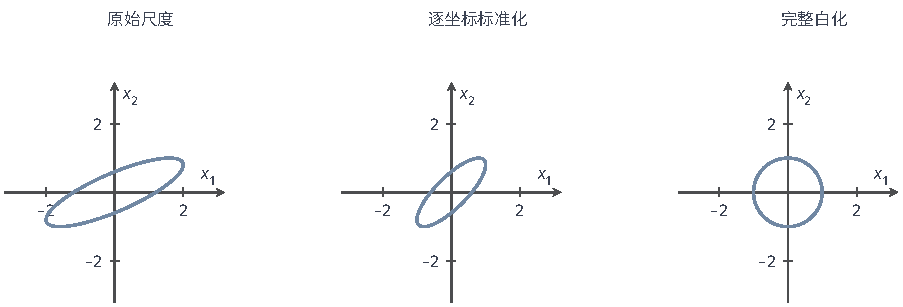
\includegraphics[width=152.834mm]{figures/05-neural-network-models/00-shared/tikz/training-whitening/figure.pdf}
  \caption{以$\bm C=\left(\begin{smallmatrix}4&1.6\\1.6&1\end{smallmatrix}\right)$构造二维协方差椭圆。左图为原尺度，中图分别除以各坐标标准差，边际尺度相同但相关系数仍为0.8；右图用精确逆平方根白化后成为圆。曲线是解析示意，不是抽样散点或实验结果；忽略稳定项且不加入可学习仿射。}
  \label{fig:training-whitening}
\end{figure*}
\FloatBarrier

白化能处理逐坐标缩放保留的相关性，但协方差需要更多观测和矩阵计算，噪声方向还可能被过度放大\scite{huang2018dbn,huang2019iternorm}若将这个变换嵌入网络层，可学习仿射还可能重新引入相关性。固定输入白化使用保存的训练变换，隐藏响应若随参数改变，则需要相应网络内处理。

\paragraph{网络内的白化层。}

若希望持续处理隐藏特征之间的相关性，可以把白化嵌入网络层，但需要在前向计算协方差，并在反向处理该矩阵的依赖。\term{去相关批归一化}（DBN）采用ZCA白化，分组实现减少矩阵规模但舍去组间相关性；\term{迭代归一化}（IterNorm）用矩阵迭代近似逆平方根，避免直接特征分解。两者利用比对角标准化更完整的方向关系，也增加矩阵存储、统计误差与近似选择。这里的矩阵迭代处理协方差，与Muon对更新奇异值整形的目标不同。

\subsubsection{批归一化}
\label{sec:training-batchnorm-family}
\label{sec:training-batchnorm}
\label{sec:training-batchnorm-variants}
\label{sec:training-other-batchnorm}
\label{sec:training-batch-renorm}
\label{sec:training-online-powernorm}
\label{sec:training-conditional-norm}
\label{sec:training-temporal-batchnorm}
\label{sec:training-batch-channel-normalization}
批归一化用同一特征或通道的多个观测建立参照。相关方法围绕这一批统计机制，调整统计伙伴、训练与推理的参照、历史状态或输出仿射。

如果同一通道的整体响应尺度随训练变化，可以用共同统计伙伴提供尺度参照，并让网络学习输出幅度。代价是单个样本的计算与其他伙伴耦合，这又联系到第\ref{sec:training-inexact-gradients}节的批量组织。\term{批归一化}（batch normalization, BatchNorm）让同一特征在当前批量中的观测共同决定尺度。对全连接层$\bm X\in\mathbb R^{b\times d}$，固定特征$j$，统计$\{X_{i,j}:i=1,\ldots,b\}$；对卷积张量，固定通道$j$，再把批量与空间位置一起统计。每个特征或通道有一组$\gamma_j,\zeta_j$\scite{ioffe2015batchnorm}

以卷积通道为例，训练时计算
\begin{equation}
  \begin{aligned}
  \mu_j&=\frac1{bhw}\sum_{i,u,v}X_{i,j,u,v},\qquad
  v_j=\frac1{bhw}\sum_{i,u,v}(X_{i,j,u,v}-\mu_j)^2,\\
  Y_{i,j,u,v}&=\gamma_j\frac{X_{i,j,u,v}-\mu_j}{\sqrt{v_j+\epsilon}}+\zeta_j\text{。}
  \end{aligned}
  \label{eq:training-batchnorm}
\end{equation}
训练时用本批的$\mu_j,v_j$计算输出，所以一个样本的输出依赖其他统计伙伴。同时维护供推理使用的\term{运行均值}（running mean）和\term{运行方差}（running variance），即随训练批次更新、保存在模型中的滑动统计量。令$\rho\in[0,1)$为旧统计量的保留系数，一种更新约定为
\begin{equation}
  \begin{aligned}
    \bar\mu_j^{(t)}&=\rho\bar\mu_j^{(t-1)}+(1-\rho)\mu_j^{(t)},\\
    \bar v_j^{(t)}&=\rho\bar v_j^{(t-1)}+(1-\rho)\widetilde v_j^{(t)}\text{。}
  \end{aligned}
  \label{eq:training-batchnorm-running}
\end{equation}
这里$t$标记训练批次。式\eqref{eq:training-batchnorm}用于当前前向的$v_j^{(t)}$以$m=bhw$为分母；更新运行方差所用的$\widetilde v_j^{(t)}$则须按实现约定：可以使用同一批方差，也可以在$m>1$时使用$m v_j^{(t)}/(m-1)$。后一种在独立同分布观测下是无偏方差估计，空间相关性会改变这一性质；当前前向仍使用分母$m$的批统计。接口中的momentum可能指$\rho$，也可能指新批权重$1-\rho$，需查明定义。

采用运行统计的常规BN在推理时冻结$\bar\mu_j,\bar v_j$，既不重新计算推理批次的均值、方差，也不继续更新滑动统计；只把式\eqref{eq:training-batchnorm}中的$\mu_j,v_j$换成保存值。因而同一输入的BN输出不再随推理批次的伙伴改变。运行统计累积历次批统计，初始化、采样和训练期间的参数变化都进入这份估计；在最终参数下遍历数据得到的统计则使用另一组响应。关闭运行统计跟踪等配置会改为其他参照，实际计算由该配置决定。

若统计集合只有一个元素，中心化后为0，归一化不能保留该元素的变化。卷积中即使$b=1$，空间位置仍可提供多个元素，但高度相关的位置并不等同于独立样本。小批量、单类别采样或相邻视频帧都可能使统计量偏离预期使用分布。统计伙伴的相关性与组成决定这份尺度参照是否适合实际输入。

固定运行统计量后，BatchNorm是通道仿射变换，可与前面的线性层或卷积折叠，第\ref{sec:snn-conversion}节给出公式。训练时的批统计随输入变化，求导包含这份依赖，因此对应一张动态计算图。验证、推理和模型导出需要采用一致模式。

BatchNorm调节表示尺度，并通过重参数化影响梯度与优化形状。原始工作用内部协变量偏移说明动机，后续研究指出训练收益不能简单归因于阻止中间分布变化，在所研究设置中还体现为更平滑的优化行为。这些研究中的模型、数据与优化设置限定了所支持的解释\scite{santurkar2018batchnorm}

\paragraph{批统计范围的调整。}

批归一化的统计伙伴未必与一次参数更新使用的样本集合一致。同步与幽灵批归一化分别扩大和缩小伙伴集合，处理局部批量不足与过大统计集合的问题。分布式训练中，每台设备的局部批量可能很小。\term{同步批归一化}（synchronized BatchNorm, SyncBatchNorm）跨指定设备集合共同统计。设设备$r$有$N_r$个统计元素、均值$\mu_r$和方差$v_r$，正确合并为
\begin{equation}
  \begin{aligned}
    N&=\sum_rN_r,\qquad \mu=\frac{\sum_rN_r\mu_r}{N},\\
    v&=\frac1N\sum_rN_r[v_r+(\mu_r-\mu)^2]\text{。}
  \end{aligned}
  \label{eq:training-sync-batchnorm}
\end{equation}
设备内方差与设备间均值差共同形成合并方差，均值也按元素数加权。同步扩大伙伴并增加通信，观测间已有的相关性继续保留。大型批量检测中的同步统计是其典型使用情形\scite{peng2018megdet}

当优化批量很大，又希望保留较小统计集合时，\term{幽灵批归一化}（Ghost BatchNorm）将同一次优化批量分成较小子组，各组分别计算归一化统计，再合并梯度更新。它区分“有多少样本决定一次更新”与“有多少样本共同决定一次归一化”，两种批量分别进入前向统计和参数更新\scite{hoffer2017ghostbn}

这两种做法的优势是可以单独选择统计批量，而不必同步改变优化批量。SyncBatchNorm增加通信，Ghost BatchNorm增加统计波动；扩大或缩小伙伴都需要验证。若困难来自训练与推理参照不同，还需要下面的统计校正。

\paragraph{参照批量与训练推理校正。}

小批量或非独立采样可能使当前统计波动，训练与推理的参照又不同。相关方法通过调整参考批量或校正批统计，缓解参照差异\scite{salimans2016gantechniques,ioffe2017batchrenorm}\term{虚拟批归一化}（virtual batch normalization, VBN）将当前样本与固定参考批量结合，减少对工作批量中其他新样本的依赖；参考集合的偏差与额外计算仍会保留。这里参考批量参与前向统计，梯度累积则合并已经算出的参数导数。

\term{批再归一化}（batch renormalization）把批标准化结果改为$\hat x=r(x-\mu_B)/\sigma_B+d$。$r$由批标准差与运行标准差之比得到，$d$由两种均值之差得到，二者均按调度裁剪并停止梯度。未裁剪时，前向等于使用运行统计；反向仍通过批内统计求导。它缓解两种参照的差异，却增加运行状态和校正范围的选择。

\Needspace{18\baselineskip}
\paragraph{流式与历史统计。}

在流式或微批量条件下，\term{在线归一化}（OnlineNorm）沿样本流维护统计并设计相应的反向校正；\term{PowerNorm}用运行平方均值和近似反向处理管理Transformer中的批尺度波动\scite{chiley2019onlinenorm,shen2020powernorm}它们让参照跨时间积累，代价是状态次序、重置规则与分布变化后的滞后。前向历史与反向校正共同定义这些方法，因果预测中的统计还限制在当时已经到达的观测内。

\paragraph{条件批归一化与空间调制。}

生成任务要让共享内容表示随条件改变，固定仿射只能提供同一组尺度。\term{条件归一化}让条件$\bm c$产生$\bm\gamma(\bm c),\bm\zeta(\bm c)$，计算$\bm y=\bm\gamma(\bm c)\odot\hat{\bm x}+\bm\zeta(\bm c)$。条件化改变仿射参数的来源，底层统计伙伴仍由所选归一化决定；同一思路也可用于后面的层归一化与实例归一化。图~\ref{fig:training-conditional-norm}展示内容与条件两条路径。
\begin{figure}[htbp]
  \centering
  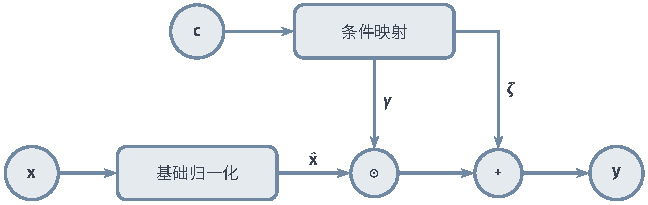
\includegraphics[width=109.792mm]{figures/05-neural-network-models/00-shared/tikz/training-conditional-norm/figure.pdf}
  \caption{条件归一化的共同计算图。内容路径产生$\hat{\bm x}$，条件映射产生缩放$\bm\gamma$与偏移$\bm\zeta$，圆形节点分别表示逐元素乘法与加法。条件既可以是风格统计，也可以是类别、文本或时间等输入；空间调制还让仿射参数随位置变化。}
  \label{fig:training-conditional-norm}
\end{figure}
\FloatBarrier

条件BatchNorm保留批统计，让类别、文本等条件产生通道仿射参数。\term{空间自适应归一化}（SPADE）让语义布局产生随位置变化的缩放与偏移，把布局条件送回归一化后的特征。原工作使用同步批统计，因此在这里介绍；如果底层换为InstanceNorm，则应按实例范围理解。条件编码增加参数与计算，且仍需核对底层统计在训练和推理中的行为\scite{park2019spade}

\paragraph{时间展开的批统计。}

脉冲分布随时间变化时，\term{时间展开批归一化}（BNTT）为不同时间步设置统计与参数，使各时刻拥有相应尺度参照。它保持批归一化的统计范围，增加了时间索引，因此归入本类。代价是更多状态，推理窗口改变时还需处理未训练时刻；当前输出的统计只使用预测时已经给定的输入\scite{kim2021bntt}

\paragraph{与通道组统计和激活的组合。}

微批量下，批尺度校正还可以与样本内的通道组处理串联。\term{批通道归一化}（BCN）采用这类组合，并与参数侧的权重标准化配合。它增加了样本内统计，但保留批或历史参照的依赖；详细效果取决于统计与运行状态的实现，批/历史参照与组内计算分别进入完整模块\scite{qiao2020wsbcn}

\term{EvoNorm}把归一化与非线性共同设计。B系列使用批统计，B0还将批方差与实例方差结合，因而具有跨样本依赖，也需维护推理统计。它与先BatchNorm再激活的计算不同；替换时需核对整个模块。使用样本内组统计的S0放在第\ref{sec:training-groupnorm}节介绍\scite{liu2020evonorm}

\subsubsection{层归一化}
\label{sec:training-layernorm-family}
\label{sec:training-layernorm}
\label{sec:training-rmsnorm}
\label{sec:training-scalenorm}
\label{sec:training-pixelnorm}
\label{sec:training-qknorm}
\label{sec:training-adaptive-layernorm}
\label{sec:training-normalization-block-designs}
\label{sec:training-normalization-placement}
\label{sec:training-other-normalization-designs}
这一类在单个样本的指定表示内部建立尺度参照，不借用其他样本。相关方法保留这一作用范围，改变是否中心化、如何计算长度以及仿射参数的来源；层归一化在残差块中的放置方式也在本类内说明。

批量组成或大小变化时，跨样本参照可能不适合当前表示。LayerNorm把尺度参照移到同一个样本表示内部，隔离其他样本对这一步局部导数的影响。逐词元计算也让参照范围不随序列长度和推理批量改变。\term{层归一化}（layer normalization, LayerNorm）对选定表示中的多个特征共同计算均值与方差。对$\bm X\in\mathbb R^{b\times n\times d}$，Transformer通常固定样本$i$与词元位置$t$，在特征维$j=1,\ldots,d$上统计，使用式\eqref{eq:training-normalization-common}，仿射参数$\bm\gamma,\bm\zeta\in\mathbb R^d$跨样本和位置共享\scite{ba2016layernorm}

其他样本和其他位置不参与当前词元的统计，训练与推理均使用当前表示。因此，逐词元LayerNorm不依赖批量组成，也不需要保存运行均值与方差。注意力、池化和损失再用各自掩码处理有效位置，LayerNorm在每个位置内部统计。

层归一化的实际范围由选定形状规定。对图像，可以选定全部通道及空间位置，也可以只在每个位置跨通道统计；两种形状会保留不同信息。整样本LayerNorm的仿射参数还可能逐元素设置，GroupNorm则通常逐通道设置，即使统计范围相同也未必是同一个完整映射。

若忽略$\epsilon$，对$\bm x$加同一个常数或乘以同一个正数，不改变中心化后的标准化表示。它消去的是共同平移与尺度，保留相对特征关系。若任务需要共同幅值，应依靠保留路径或其他设计保存，固定$\gamma,\zeta$只规定公共仿射，逐输入被消去的幅度需要由其他路径提供。

\paragraph{均方根归一化。}

式\eqref{eq:training-normalization-jacobian}中的中心化会消去共同平移方向；如果只想管理幅度，这一步未必必要。RMSNorm保留未中心化表示，再由平方幅度决定尺度。\term{均方根归一化}（root mean square normalization, RMSNorm）对$\bm x\in\mathbb R^d$采用
\begin{equation}
  y_j=\gamma_j\frac{x_j}{\sqrt{d^{-1}\sum_{k=1}^d x_k^2+\epsilon}}\text{。}
  \label{eq:training-rmsnorm}
\end{equation}
基本形式不减均值，也不加入偏移参数。它使表示对共同正尺度变化近似不敏感，但不对共同平移不敏感；分母同时包含方差与均值平方，因为$d^{-1}\sum_jx_j^2=v+\mu^2$\scite{zhang2019rmsnorm}

\begin{example}[减去均值改变了哪些信息]
  \label{ex:training-layer-rms}
  取两个仅相差共同偏移的向量：
  \[
    \bm x=(1,2,3)^{\top},\qquad \bm x'=(11,12,13)^{\top}\text{。}
  \]
  忽略$\epsilon$并令仿射缩放为1，LayerNorm的两次输出都为
  \[
    (-\sqrt{3/2},0,\sqrt{3/2})^{\top}\text{。}
  \]
  共同偏移10被消去。RMSNorm分别给出$\bm x/\sqrt{14/3}$与$\bm x'/\sqrt{434/3}$，结果不同。二者都控制尺度，但保留的信息不同。
\end{example}

RMSNorm省去中心化与偏移，统计操作较少，并保留共同偏移对方向和分母的影响；共同正缩放在忽略稳定项时仍被消去，原始幅度因而需要另行保存。是否比LayerNorm更适合，应结合任务需要的信息与实际算子成本判断。

\paragraph{部分统计与整体长度。}

\term{部分RMSNorm}（pRMSNorm）只用特征子集估计均方根，以减少统计量的归约计算。节省来自少统计一些元素，风险是子集不能代表完整幅度，算子实现也决定它是否实际更快。

有些任务关心向量方向，或希望仅管理局部响应的幅度。\term{ScaleNorm}采用$\bm y=g\bm x/\max(\lVert\bm x\rVert_2,\epsilon)$，只学习一个整体长度$g$；\term{FixNorm}固定嵌入长度，普通L2归一化则得到单位向量。它们计算简单，适合将方向用于相似性，但会删除绝对幅度；逐特征可学习缩放与整体长度并不等价\scite{nguyen2019scalenorm}

\paragraph{图像位置与注意力向量的长度。}

\term{PixelNorm}在单个图像位置跨通道计算均方根，基本形式没有仿射与中心化；PGGAN用它管理生成器特征幅度。按统计范围，它与逐位置RMS缩放相近，所以放在层内特征尺度方法中；其统计只覆盖当前空间位置的通道，原始幅度仍受该缩放影响\scite{karras2018pggan}

\term{查询--键归一化}（QKNorm）在每个注意力头内归一化单个查询和键向量的长度，以可学习系数缩放余弦得分。它同样只处理当前向量的特征维，目的是减少长度增长引起的Softmax饱和。它管理注意力评分的尺度，残差块的表示统计属于另一条路径，查询键归一化之后还需配置评分温度\scite{henry2020qknorm}

\paragraph{条件层归一化。}

当输出需要随类别、文本或时间等条件变化时，\term{自适应LayerNorm}（AdaLN）在层统计之后使用条件仿射，条件RMSNorm则保留均方根统计。二者沿用图~\ref{fig:training-conditional-norm}的两条路径，改变的是仿射来源。DiT中的AdaLN-Zero还把残差条件门初始化为0，让初始分支较弱；“Zero”指门与相应仿射的初始化，训练会继续调整这些参数。底层统计、条件网络与残差门须分别说明\scite{peebles2023dit}

\paragraph{残差块中的放置与尺度配合。}

层归一化的统计范围不变，放置位置与残差尺度仍会改变第\ref{sec:training-gradient-propagation}节的Jacobian矩阵连乘\scite{shleifer2021normformer,wang2022deepnet}Pre-LN残差块形如$\bm h'=\bm h+F(\operatorname{LN}(\bm h))$，Post-LN形如$\bm h'=\operatorname{LN}(\bm h+F(\bm h))$。前者保留未经过本步归一化的直接路径，后者对合并结果共同归一化；输出尺度、梯度路径和初始化需求不同，第\ref{sec:transformer-residual-normalization}节展开了具体结构。

直接路径有利于把梯度送回较早层，但Pre-LN分支仍可能很弱，整体尺度仍需管理；Post-LN约束合并后的表示，却让归一化导数进入每个块的传播。选择位置应配合残差尺度与初始化。

NormFormer增加归一化位置与尺度调节，DeepNorm配合残差缩放和初始化支持更深堆叠；二者通过完整块组织、残差系数和初始参数共同作用于传播。增加操作或改变系数也有成本，应检查完整计算图与初始化条件。

\subsubsection{实例归一化}
\label{sec:training-instancenorm}
\label{sec:training-adaptive-instancenorm}
\label{sec:training-frn-pixelnorm}
\label{sec:training-frn}
图像外观可能随样本变化，共享批统计未必能去掉每幅图各通道的独有尺度。InstanceNorm在该样本通道内部建立参照，代价是可能同时去掉有用的外观幅度。图像中，某个通道的均值与对比度可能更多描述风格，而非内容。\term{实例归一化}（instance normalization, InstanceNorm）固定样本$i$和通道$j$，只在$(u,v)$上计算均值与方差。常见实现不使用跨样本运行统计，训练与推理都归一化当前输入；可选仿射参数按通道共享\scite{ulyanov2016instancenorm}

它把每个样本的每个通道都调整到相近统计尺度，有利于去除某些外观差异，却也可能消去任务需要的亮度或强度。若空间只剩一个元素，中心化会退化；若启用运行统计，推理性质又不同。空间形状、仿射参数与运行统计配置共同确定这张映射。

\paragraph{自适应实例归一化。}

若希望内容保留空间结构，同时采用另一幅图的通道统计，可以在实例标准化后重设均值与幅度。\term{自适应实例归一化}（AdaIN）用风格特征的通道均值和标准差重设内容统计，形式为$\sigma(\bm s)\odot[\bm x-\mu(\bm x)]/\sigma(\bm x)+\mu(\bm s)$，零方差需稳定处理。它保留实例统计范围，把固定仿射换为风格统计；这种匹配方便注入外观条件，感知风格的相似程度还由后续生成与评价确定\scite{huang2017adain}

\paragraph{不减均值的滤波响应归一化。}

如果希望在每个样本的每个通道内管理幅度，又保留共同偏移的影响，可以在相同空间范围内改用未中心化的平方幅度。\term{滤波响应归一化}（FRN）沿这一范围计算均方根，不减均值，再使用仿射和可学习阈值激活。按作用范围将它放在本类，但它与标准InstanceNorm的映射不同；完整模块还包含激活，空间很小时稳定项与信息损失尤须注意\scite{singh2020frn}

\subsubsection{组归一化}
\label{sec:training-groupnorm}
\label{sec:training-instance-groupnorm}
\label{sec:training-evonorm}
统计集合太小会使尺度估计不稳定，全部通道混合又可能过于粗糙。GroupNorm在样本内部选择中间大小的通道组，在信息粒度与统计元素数之间取舍。\term{组归一化}（group normalization, GroupNorm）将$c$个通道预先划为$g$组，在单个样本内对组内通道及空间位置共同统计。等分时要求$c$能被$g$整除，每组统计元素数为$(c/g)hw$，仿射参数通常仍逐通道设置\scite{wu2018groupnorm}

当$g=c$时，统计范围与InstanceNorm相同；当$g=1$时，与整样本LayerNorm相同。完整映射仍需核对仿射参数和运行统计配置。组数控制哪些特征共同决定尺度，相应组数与任务信息、形状和训练共同决定输出表现。

\paragraph{组统计与非线性的联合计算。}

组归一化后再接激活，会让两步导数共同进入反向传播。上文EvoNorm系列中的S0直接联合这两部分，采用$y_j=\gamma_jx_j\sigma(a_jx_j)/\sqrt{v_G+\epsilon}+\zeta_j$，其中$v_G$是样本内通道组的中心化方差，$a_j$可学习，$\sigma$为Sigmoid。它使用组统计，分子却不减均值，中心化分母与未中心化分子共同形成这一模块，另接同样激活又会改变其输出和导数。

图~\ref{fig:training-normalization-axes}用同一构造数据比较已讨论的批、层、实例和组统计。图中采用常见轴名$N,C,H,W$，分别对应前文的批量$b$、通道$c$、高$h$和宽$w$；元素索引写作$(n,c,h,w)$。图将$(h,w)$展开为行、通道$c$排成列，两张小表分别表示样本$n=1,2$。轮廓内的着色格共同计算均值与方差，圈出的目标元素始终不变，因而可以直接比较哪些伙伴被加入或排除。

BN固定$c$，跨$n,h,w$统计；IN固定$n,c$，只跨$h,w$，并不跨实例。GN固定$n$和通道组，跨组内$c$及$h,w$。图中的LN明确采用图像整样本约定：固定$n$，统计全部$C,H,W$。Transformer的逐词元LN则固定样本$n$和词元位置$t$，只沿特征$C$（前文记为$d$）统计；序列中的统计伙伴因而与图示整幅图像不同。选择统计伙伴改变数值结果，也改变式\eqref{eq:training-normalization-jacobian}中哪些特征共同参与导数。
\begin{figure*}[htbp]
  \centering
  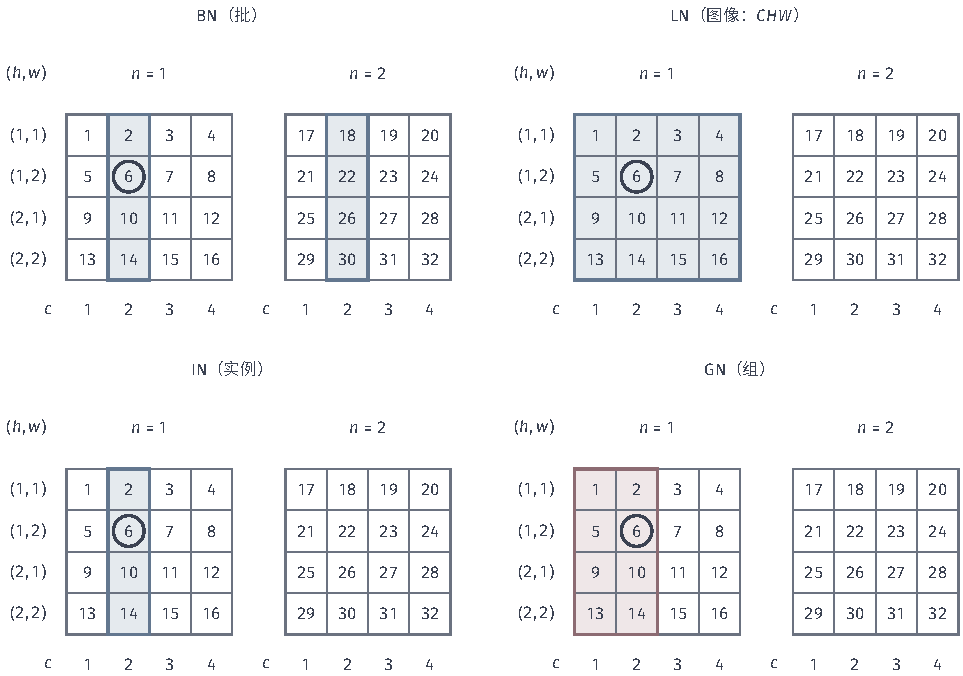
\includegraphics[width=163.146mm]{figures/05-neural-network-models/00-shared/tikz/training-normalization-axes/figure.pdf}
  \caption{在$N=2,C=4,H=W=2$的图像张量上，对同一元素$X_{1,2,1,2}=6$比较统计伙伴。按样本、空间行、通道的展示顺序填入教学数值1至32，每行标出$(h,w)$；并非按张量存储顺序编号。蓝、紫、青、橙分别标出BN、LN、IN、GN的统计集合，边界轮廓及$n$、$c$、$(h,w)$标签提供颜色之外的读法，深色圈为目标元素。GN取通道组$\{1,2\}$；LN统计整幅图像的$CHW$，不是Transformer逐词元的特征维LN；图中未加入仿射变换。}
  \label{fig:training-normalization-axes}
\end{figure*}
\FloatBarrier

表~\ref{tab:training-normalization-axes}将范围写成索引，便于在不同张量排列下实现。位置、通道和批量放在第几个维度可以改变，但统计伙伴的语义必须保持。
\begin{table*}[htbp]
  \centering\small
  \begin{tabularx}{\linewidth}{@{}p{35mm}p{43mm}X@{}}
    \toprule
    方法 & 固定的索引 & 共同计算统计量的索引 \\
    \midrule
    BatchNorm & 通道$j$ & 样本$i$、位置$u,v$ \\
    LayerNorm（整样本） & 样本$i$ & 通道$j$、位置$u,v$ \\
    LayerNorm（每位置） & 样本$i$、位置$u,v$ & 通道$j$ \\
    InstanceNorm & 样本$i$、通道$j$ & 位置$u,v$ \\
    GroupNorm & 样本$i$、通道组 & 组内通道$j$、位置$u,v$ \\
    \bottomrule
  \end{tabularx}
  \caption{在$\bm X\in\mathbb R^{b\times c\times h\times w}$上比较基本统计范围。每位置LayerNorm与序列中的逐词元形式对应；整样本形式与$g=1$的GroupNorm仅在统计范围上相同。RMSNorm也需明确形状，但统计的是平方均值而非中心化方差。}
  \label{tab:training-normalization-axes}
\end{table*}
\FloatBarrier

\subsection{参数归一化}
\label{sec:training-parameter-normalization-methods}
\label{sec:training-weight-normalization-methods}
前面的基本方法管理表示统计，权重方法则直接改变线性映射的参数化。权重自身提供尺度参照，向量长度、滤波器均值方差和整矩阵最大放大分别对应不同约束。

\subsubsection{权重归一化}
\label{sec:training-weightnorm}
第\ref{sec:training-curvature}节指出重参数化可以改变更新几何。WeightNorm把长度与方向作为不同变量，让优化器分别调整两种自由度，无需估计激活的批统计。\term{权重归一化}（weight normalization, WeightNorm）把非零权重向量写为
\begin{equation}
  \bm w=g\frac{\bm v}{\lVert\bm v\rVert_2}\text{，}
  \label{eq:training-weightnorm}
\end{equation}
其中$g$是可训练标量，$\bm v$决定方向。对卷积可按输出滤波器分别使用，对线性层可按行使用。这份方向/长度参数化由权重决定，激活均值继续取决于输入与映射\scite{salimans2016weightnorm}

设原权重梯度为$\bm a=\nabla_{\bm w}\mathcal L$，链式法则给出$\partial\mathcal L/\partial g=\bm v^{\top}\bm a/\lVert\bm v\rVert_2$，以及
\begin{equation}
  \nabla_{\bm v}\mathcal L
  =\frac{g}{\lVert\bm v\rVert_2}
    \left(\bm I-\frac{\bm v\bm v^{\top}}{\lVert\bm v\rVert_2^2}\right)\bm a\text{。}
  \label{eq:training-weightnorm-gradient}
\end{equation}
方向梯度包含垂直投影，因此更新$g,\bm v$与直接更新$\bm w$的轨迹不同。$\bm v=\bm0$需要由初始化和数值处理避免。行长度与整矩阵最大放大还具有不同口径：例如两行都为$(1,0)$时，矩阵谱范数为$\sqrt2$，超过单行长度1。

\subsubsection{权重标准化}
\label{sec:training-weight-standardization}
滤波器自身的均值和尺度会影响初始及后续响应，批量很小时也难以依靠稳定批统计补偿。WS直接处理权重分布，使这一尺度管理与当前样本伙伴分开。\term{权重标准化}（weight standardization, WS）不只分离长度，还对每个滤波器的权重减均值并按标准差缩放。将第$i$个输出滤波器展平为$d$个元素，采用
\begin{equation}
  \begin{aligned}
    \mu_i^W&=\frac1d\sum_jW_{i,j},\qquad
    v_i^W=\frac1d\sum_j(W_{i,j}-\mu_i^W)^2,\\
    \bar W_{i,j}&=\frac{W_{i,j}-\mu_i^W}{\sqrt{v_i^W+\epsilon}}\text{。}
  \end{aligned}
  \label{eq:training-weight-standardization}
\end{equation}
实际卷积使用$\bar{\bm W}$，反向穿过权重统计更新原始$\bm W$。它管理的是滤波器参数分布，与在样本或位置上统计的GroupNorm可以组合。微批量训练中的WS与BCN研究了这类互补作用，权重与样本统计分别改变映射的不同环节\scite{qiao2020wsbcn}

WS控制滤波器统计，输出激活则继续依赖输入与空间结构。

\paragraph{缩放权重标准化。}

带增益和扇入校正的缩放权重标准化继续作用于滤波器参数。NFNet把它与残差信号尺度、激活修正和自适应梯度裁剪配合，以减少通常的激活批统计依赖。这些尺度、连接与裁剪共同构成完整模型，实验中的收益对应这组设计\scite{brock2021nfnet}

\subsubsection{谱归一化}
\label{sec:training-spectralnorm}
激活方差或每行长度并不控制所有方向的最大放大。第\ref{sec:training-gradient-propagation}节使用的算子上界，需要与最大奇异值相关的控制，谱归一化因此关注线性映射的最大放大。\term{谱归一化}（spectral normalization）对非零矩阵采用$\bar{\bm W}=\bm W/\sigma_{\max}(\bm W)$，$\sigma_{\max}$为最大奇异值。计算中常以幂迭代近似：交替用$\bm W^{\top}\bm u$与$\bm W\bm v$并归一化，再估计$\bm u^{\top}\bm W\bm v$\scite{miyato2018spectral}

若估计值小于真实最大奇异值，除法后的真实算子范数仍可能超过1，严格的算子上界需要控制这份估计误差。零矩阵与很小估计还需稳定处理，是否沿估计向量求导也应按实现说明。

若每层算子范数已受约束，且激活是已知Lipschitz映射，普通串联网络的输入敏感度可由尺度乘积控制。残差求和、归一化和注意力需另行计入。卷积核展平矩阵的谱范数与完整空间卷积算子通常不同，整网敏感度应据实际卷积算子及其他模块合计。谱归一化控制最大方向，WeightNorm分离方向与长度，WS调整滤波器均值和方差，三者目的不同。

\subsection{其他归一化方法}
\label{sec:training-other-normalization}
有些方法混合多个统计范围，有些围绕可逆变换、图结构或通道竞争定义尺度，这些计算使用的对象或范围超出了前述基本形式。这里按具体计算作补充；是否采用仍要对应实际训练困难，并评估信息损失、状态与计算成本。

\subsubsection{混合统计与局部响应}
\label{sec:training-normalization-combinations}
\label{sec:training-switchable-bcn}
固定统计范围未必适合每一层。\term{可切换归一化}（SwitchableNorm）分别计算批、层、实例统计，学习均值和方差的凸组合。它同时使用多个范围，因而不放入单一基础类别。统计混合增加计算，只要批分量存在，就仍需处理跨样本或历史依赖；这与第\ref{sec:training-batchnorm-family}节中BCN串联不同，后者依次执行映射\scite{luo2019switchablenorm}

\term{局部响应归一化}（local response normalization, LRN）属于局部除法竞争。第\ref{sec:cnn-alexnet}节中AlexNet的一种形式为$y_j=x_j/(k_0+a\sum_{r\in N(j)}x_r^2)^\beta$，这里省略样本与空间索引，$N(j)$是邻近通道，$k_0>0,a\geq0,\beta>0$。强响应会抑制邻域幅度；它既不减均值，也不按前述批、层、实例或固定通道组计算标准差，它形成了另一种局部响应函数。

\subsubsection{可逆仿射}
\label{sec:training-actnorm}
可逆生成模型需要逐样本可逆、且行列式容易计算的尺度变换。\term{ActNorm}用首批数据初始化通道仿射$Y_{i,j,u,v}=s_jX_{i,j,u,v}+b_j$，之后直接学习$s_j,b_j$，不再重估每批统计。取$s_j=\exp(a_j)$可保证非零尺度；单样本对数Jacobian行列式为$hw\sum_j\log|s_j|$。其优势是逐样本计算一致、可逆性明确，代价是初始数据影响起点，后续输出不再保证零均值和单位方差\scite{kingma2018glow}

\subsubsection{通道响应与图结构}
\label{sec:training-grn-qknorm}
\label{sec:training-graph-temporal-norm}
\label{sec:training-global-response-normalization}
\term{全局响应归一化}（GRN）在ConvNeXt V2中比较各通道的空间L2响应，再将相对强度用于残差调制。它管理通道竞争，不强制单位方差；其映射同时使用空间响应与通道间的相对比较\scite{woo2023convnextv2}

图模型的统计还需尊重每张图的边界。\term{GraphNorm}逐图、逐特征统计，以可学习系数决定去掉多少图均值；\term{PairNorm}中心化节点后统一缩放总体长度，管理节点间距离；\term{MessageNorm}把聚合消息的长度调整为相对节点状态的可学习比例。它们分别处理图级偏移、过平滑与消息幅度，各自参照图均值、节点距离或消息相对长度\scite{cai2021graphnorm,zhao2020pairnorm,li2020deepergcn}

这些方法分别调整保留下来的图偏移、节点距离或消息幅度。图边界与节点分布、节点间差别、消息与状态的相对长度，因而成为各自的诊断对象；任务表现再显示这些调整是否适合当前预测。

\subsubsection{统计归一化的替代}
\label{sec:training-normalization-substitutes}
尺度也可以由不使用样本统计的非线性压缩管理。2025年的\term{动态Tanh}（DyT）以$\bm\gamma\odot\tanh(a\bm x)+\bm\zeta$替代部分Transformer归一化层，不计算当前表示的均值或方差，因此不能按前述统计范围归类。它展示了另一种尺度控制路线，也要求保留其配套设计和实验范围；替换效果对应论文中的模块、配套设置与任务\scite{zhu2025dyt}

\subsection{归一化方法的比较与选择}
\label{sec:training-normalization-comparison}
比较方法时，可以回到第\ref{sec:training-curvature}节的方向尺度与第\ref{sec:training-gradient-propagation}节的Jacobian矩阵连乘。特征归一化改变输入或隐藏表示，参数归一化改变生成映射的权重；二者可能共同改善尺度，但即使输出方差相近，统计依赖与参数化仍可产生不同导数。选择时需同时检查以下维度：
\begin{itemize}
  \item \textbf{作用对象。} 调整的是输入、隐藏特征还是权重，决定直接改变计算图的哪一部分。
  \item \textbf{统计范围。} 跨样本、表示内部、单通道空间或通道组，决定计算依赖和统计元素数；白化还需估计特征间的协方差。
  \item \textbf{保留信息。} 是否去均值、固定长度或去相关，决定共同偏移、幅度与方向关系怎样改变。
  \item \textbf{执行条件。} 固定训练参照、当前统计还是运行状态，决定训练推理是否一致，以及通信、矩阵计算和条件网络的成本。
\end{itemize}

表~\ref{tab:training-normalization-basic-comparison}比较五类特征方法，表~\ref{tab:training-normalization-special-comparison}比较参数方法，表~\ref{tab:training-normalization-extended-comparison}列出具体方法的归属。分类先固定作用对象和统计范围，再比较范围内的公式差异；条件仿射与残差块位置属于相应基础方法的扩展，不另列为一种统计类别。
\begin{table*}[htbp]
  \centering\small
  \begin{tabularx}{\linewidth}{@{}p{24mm}p{43mm}p{35mm}X@{}}
    \toprule
    类别 & 统计或尺度对象 & 主要处理 & 优势与主要边界 \\
    \midrule
    白化 & 观测集合内的特征协方差 & 中心化与协方差变换 & 去相关；矩阵计算与统计误差较大 \\
    批归一化 & 同通道的批量与空间位置 & 批均值、方差或历史尺度 & 共享尺度参照；批伙伴与推理状态需核对 \\
    层归一化 & 单表示的指定特征维 & 方差、均方根或向量长度 & 隔离其他样本；变体保留的信息不同 \\
    实例归一化 & 单样本单通道的空间位置 & 方差或未中心化平方幅度 & 管理样本外观；可能删去有用强度 \\
    组归一化 & 单样本组内通道与空间位置 & 组内统计 & 不依赖批量；组数改变信息粒度 \\
    \bottomrule
  \end{tabularx}
  \caption{按作用范围比较特征归一化。白化可采用训练集固定参照或网络内动态协方差；批归一化通常在推理时使用运行统计。其余类别按基本形式使用当前表示，具体变体还需核对中心化、仿射与状态。}
  \label{tab:training-normalization-basic-comparison}
\end{table*}
\FloatBarrier

\begin{table*}[htbp]
  \centering\small
  \begin{tabularx}{\linewidth}{@{}p{31mm}p{51mm}X@{}}
    \toprule
    方法 & 管理的参数性质 & 优势与主要边界 \\
    \midrule
    WeightNorm & 分开权重方向与长度 & 不需批统计；行长度不控制整矩阵谱范数 \\
    WS及缩放变体 & 滤波器均值与方差、增益与扇入尺度 & 与激活统计分开；不保证输出尺度 \\
    SpectralNorm & 最大奇异值 & 管理最大线性放大；近似及算子定义需明确 \\
    \bottomrule
  \end{tabularx}
  \caption{参数归一化的比较。三者不依赖当前批量，但重参数化或归一化改变优化轨迹；缩放WS还需核对具体结构中的配套系数。}
  \label{tab:training-normalization-special-comparison}
\end{table*}
\FloatBarrier

\begin{table*}[htbp]
  \centering\small
  \begin{tabularx}{\linewidth}{@{}p{26mm}p{85mm}X@{}}
    \toprule
    归属 & 方法与相关扩展 & 需要单独核对的改动 \\
    \midrule
    特征：白化 & ZCA、DBN、IterNorm & 固定或当前协方差、分组与矩阵近似 \\
    特征：批归一化 & BatchNorm；Sync／Ghost BN、VBN、Batch Renorm、OnlineNorm、PowerNorm、BNTT；条件BN、SPADE、BCN、EvoNorm-B & 伙伴、运行状态、时间索引、条件仿射或联合模块 \\
    特征：层归一化 & LayerNorm；RMSNorm、pRMSNorm、ScaleNorm、FixNorm、PixelNorm、QKNorm；AdaLN、条件RMSNorm；Pre／Post-LN、NormFormer、DeepNorm & 中心化与长度、条件来源、评分尺度和块位置 \\
    特征：实例归一化 & InstanceNorm、AdaIN、FRN & 风格统计、均方根与阈值激活 \\
    特征：组归一化 & GroupNorm、EvoNorm-S0 & 组数与联合非线性 \\
    参数归一化 & WeightNorm、WS、缩放WS、SpectralNorm & 重参数化、增益与算子尺度 \\
    其他方法 & SwitchableNorm、LRN、ActNorm、GRN、GraphNorm、PairNorm、MessageNorm、DyT & 混合范围、局部竞争、可逆性、图边界或替代统计 \\
    \bottomrule
  \end{tabularx}
  \caption{具体方法的归属对照。前五行对应第\ref{sec:training-feature-normalization-methods}节的五类，参数方法见第\ref{sec:training-parameter-normalization-methods}节，其他方法见第\ref{sec:training-other-normalization}节。共同范围内仍有公式与模块差异；SPADE的底层统计可配置，BCN含串联组统计，Pre／Post-LN等是层归一化的组织方式，DyT是替代方案。}
  \label{tab:training-normalization-extended-comparison}
\end{table*}
\FloatBarrier

实际选择从任务信息与执行条件出发。输入量纲差异可先用固定标准化处理，需要去相关时再评估白化及矩阵成本；卷积中批伙伴足够且推理运行统计可靠时，可评估BatchNorm；批量很小或组成经常改变时，可比较GroupNorm及其组数。逐词元序列表示可在层内比较LayerNorm与RMSNorm，重点核对中心化是否有益；需要管理每幅图的通道外观时，再评估InstanceNorm与条件扩展。

若目标是控制线性映射的最大放大，参数侧的谱尺度给出相应方向指标，特征方差则描述指定输入下的响应。条件、混合与特殊结构方法也应在出现对应困难后引入，并在同一数据、结构与预算下检验收益及额外成本。

\section{参数与结构的改进}
\label{sec:training-connections}

优化器处理已经产生的梯度，参数与结构的设计则决定梯度怎样形成、从哪里传回。第\ref{sec:training-gradient-propagation}节的连乘关系说明：已经在连乘中衰减的信号，需要在相应路径与因子上处理。残差、门控与跨层连接改变计算路径，初始化决定出发时的信号尺度，持续参数约束则管理训练过程中允许的映射。这些选择沿训练轨迹共同形成实际更新。

\subsection{残差连接}
\label{sec:training-residual}

式\eqref{eq:training-jacobian-chain}中若每步都只能经过可学习变换，任何一步的方向收缩都会进入长乘积。\term{残差连接}（residual connection）在可学习变换外增加直接路径，让梯度有机会绕过变换分支。设输入输出同维，写为
\begin{equation}
  \bm h^{(l+1)}=\bm h^{(l)}+a_lF_l(\bm h^{(l)}),\qquad
  \bm J_{l+1}=\bm I+a_l\bm J_{F_l}\text{。}
  \label{eq:training-residual-jacobian}
\end{equation}
其中$a_l$为分支尺度，$\bm J_{F_l}$为分支Jacobian矩阵。原来的纯变换连乘改为含恒等项的连乘；分支在初始阶段较小时，网络可以从接近恒等映射的状态开始学习调整。直接支路改变传播路径，分支尺度再控制新增变换的强度。

恒等项与分支导数相加后，仍可能发生抵消或累积放大。若$a_l\bm J_{F_l}=-\bm I$，一层Jacobian矩阵仍可为0；若每层都沿同一方向放大，连乘仍可能增长。一个粗上界为$\prod_l(1+|a_l|\lVert\bm J_{F_l}\rVert_2)\leq\exp(\sum_l|a_l|\lVert\bm J_{F_l}\rVert_2)$，它说明分支尺度和总深度需要共同考虑。初始化、归一化与尺度方案据各分支导数及其组合共同分析。

当维度改变时，路径写为$\bm P_l\bm h^{(l)}+F_l(\bm h^{(l)})$，投影$\bm P_l$代替恒等矩阵。下采样和投影可能丢失部分方向，因而需区别恒等捷径与投影捷径。第\ref{chap:convolutional-networks}章的ResNet与第\ref{chap:transformer}章的残差块均是这一框架的具体组织。

\subsection{门控连接}
\label{sec:training-gates}

恒等捷径以固定系数传递输入，其保留比例与当前内容无关。\term{门控连接}（gated connection）把路径系数变成输入相关变量，在保留原状态与使用新计算之间调节比例。一个耦合门形式为
\begin{equation}
  \bm h^{(l+1)}=(\bm1-\bm g_l)\odot\bm h^{(l)}
                   +\bm g_l\odot F_l(\bm h^{(l)}),
  \qquad\bm g_l=\sigma(G_l(\bm h^{(l)}))\text{。}
  \label{eq:training-gated-connection}
\end{equation}
门接近0时主要保留输入，接近1时主要使用新计算。Highway网络在深度方向采用此类选择，LSTM的遗忘门和输入门则在时间方向分别控制保留与写入；这些门可以独立，不一定总和为1。GRU的更新门在旧状态与候选状态之间调节比例，重置门控制候选计算对历史的使用。

把门视为当前固定值时，保留项的局部导数为$\operatorname{diag}(\bm1-\bm g_l)$。如果门依赖输入，完整Jacobian矩阵还包含$\operatorname{diag}(F_l(\bm h)-\bm h)\bm J_{g_l}$，门的变化因而也是完整导数的一部分。时间方向上，长段保留门的乘积仍可能衰减；门长期饱和还会使门参数自身难学。初始化门偏置可以改变初始保留倾向，但是否有利取决于所需记忆长度和写入需求。

\subsection{跨层连接与密集连接}
\label{sec:training-dense-connections}

深层信息不一定都应经逐层压缩后才被使用。跨层连接给后续变换直接读取早期特征的入口，同时为反向建立较短路径；拼接再决定这些信息是否保留独立坐标。残差相加要求两路表示在对应坐标上合并。跨层拼接则把来自不同层的表示同时交给后续计算。\term{密集连接}（dense connection）令第$l$层读取之前多层的特征，例如
\begin{equation}
  \bm h^{(l)}=F_l([\bm h^{(0)};\bm h^{(1)};\cdots;\bm h^{(l-1)}])\text{，}
  \label{eq:training-dense-concat}
\end{equation}
分号表示沿特征维拼接。早期特征可经较短路径进入后面层，且保留独立坐标；后续层再学习使用哪些信息。第\ref{chap:convolutional-networks}章的DenseNet通过增长率与过渡层控制通道规模。

相加不会仅因合并而增加宽度，拼接会增加宽度与激活存储。若每层新增$k$维特征，初始宽度为$d_0$，第$l$层输入宽度为$d_0+(l-1)k$；在每层采用完整线性投影到$k$维的简化模型中，总权重数为$\sum_l k[d_0+(l-1)k]=O(Lkd_0+L^2k^2)$。真实卷积、瓶颈和过渡层改变常数及规模，参数预算据这些实际宽度和投影计算。

较长的跳跃连接也可把编码器的高分辨率特征交给解码器，减少信息必须经过压缩瓶颈的程度。连接提供了可用路径，模型是否利用它仍取决于后续变换和训练目标；错误的尺寸对齐或相加语义会破坏这一作用。训练时还需保存所引用的激活，较短传播路径与所引用表示的存储分别产生便利和代价。

\subsection{参数初始化}
\label{sec:training-initialization-constraints}
\label{sec:training-initialization}

在第\ref{sec:training-gradient-propagation}节的连乘尚未被数据更新改变前，初始权重已经决定信号是否容易传播。初始化通过打破对称和安排尺度，为后续优化提供可用起点。全零初始化使同层对称单元收到相同信号，随机初始化打破对称性；尺度过大或过小，又可能让表示与梯度迅速放大或衰减。\term{方差保持初始化}（variance-preserving initialization）按输入输出连接数与激活特性设置随机权重尺度，目的是在近似独立、零均值等假设下保持前向或反向的平均平方幅度。

对线性或近似线性激活，常见Xavier尺度为$\operatorname{Var}(W_{i,j})=2/(d_{\mathrm{in}}+d_{\mathrm{out}})$；对ReLU前向传播，He尺度为$2/d_{\mathrm{in}}$。后者中的2补偿对称输入下ReLU约保留一半平方幅度的效应。卷积中的$d_{\mathrm{in}}$要计入核位置与输入通道；分组连接、残差求和和门控则需按实际结构修正。逐层方差推导见第\ref{chap:feedforward-networks}章\scite{he2015rectifiers}

\term{正交初始化}（orthogonal initialization）令方阵权重满足$\bm W^{\top}\bm W=\bm I$，线性映射保持欧氏范数；矩形权重则只能在相应子空间或行、列方向具有类似性质。\term{恒等初始化}（identity initialization）将适当的方阵设为单位矩阵，让初始线性路径直接传递状态。两者只约束初始权重，后续无约束更新会改变这些性质，非线性激活也会改变整体Jacobian矩阵。

初始参数梯度及其核矩阵描述最初可用的学习方向，起点因此影响的不仅是激活方差（参考\BookSectionRef{sec:neural-tangent-kernel}{卷3《基础、理论与可信性》第8章“深度学习的可学习性”第8.3节“基于参数梯度初始值的可学习性”}）。有限宽度网络的参数移动可能改变核与谱，训练中的实际性质再沿更新轨迹分析。

\subsection{参数约束}
\label{sec:training-parameter-constraints}

初始化改善出发时的传播，无约束更新却可能逐渐破坏它。若希望训练期间持续限制线性映射，可通过投影、结构化参数化或惩罚维持约束。这对应第\ref{sec:training-gradient-propagation}节中每一步Jacobian矩阵尺度的管理，而不是仅在第0步选择一个矩阵。

约束要写进参数生成或更新过程。暂定更新不满足硬约束时，投影会把它改成可行参数；结构化参数化从一开始就生成可行矩阵；惩罚则允许暂时甚至持续违反，只通过损失和梯度增加代价。三者分别修正暂定值、生成可行值或改变更新目标，下面沿这三个过程展开。

\subsubsection{先更新，再投影回可行集合}

设允许的参数集合为非空闭集$\bm C$，先由优化器算出暂定值$\tilde{\bm\theta}^{(t)}$，再取
\begin{equation}
  \bm\theta^{(t)}\in\argmin_{\bm z\in\bm C}
    \tfrac12\lVert\bm z-\tilde{\bm\theta}^{(t)}\rVert_2^2\text{。}
  \label{eq:training-parameter-projection}
\end{equation}
这一步寻找距离暂定值最近的可行点。闭凸集合的欧氏投影唯一，非凸集合可能存在多解。对半径$r>0$的范数球$\bm C=\{\bm w:\lVert\bm w\rVert_2\leq r\}$，投影为$\bm w=\tilde{\bm w}\min(1,r/\lVert\tilde{\bm w}\rVert_2)$，零向量保留。例如$r=2$时，暂定参数$(3,4)^{\top}$被改为$(1.2,1.6)^{\top}$；已经在球内的参数不变。这里限制的是更新后的参数，前面的梯度裁剪限制的是更新前的梯度，两者分别管理参数集合与当前梯度信号。

矩阵约束也可以直接修正奇异值。对方阵暂定权重$\tilde{\bm W}=\bm U\bm\Sigma\bm V^{\top}$的完整SVD，若要求$\sigma_{\max}(\bm W)\leq r$，就把每个奇异值改成$\min(\sigma_j,r)$；若要求$\bm W^{\top}\bm W=\bm I$，则取$\bm W=\bm U\bm V^{\top}$。这两种构造分别是对应集合的Frobenius距离投影。例如$\operatorname{diag}(1.2,0.6)$投影到谱范数不超过1的集合，得到$\operatorname{diag}(1,0.6)$；投影到正交矩阵集合则得到$\bm I$，对较小方向的处理完全不同。

实际训练在每次更新后执行该修正，并记录参数范数或正交残差。投影提供明确的可行性，但SVD等计算可能昂贵，且修正后的位移与优化器原先建议的位移不同。动量缓冲的保留或修正、预条件与投影怎样配合，共同决定下一步更新与约束几何的关系。

\subsubsection{用参数化保证每次前向都满足约束}

还可以只更新无约束变量$\bm B$，每次前向由$\bm B$生成实际权重。正尺度可写成$\exp(b)$，固定非零向量长度可写成$r\bm v/\lVert\bm v\rVert_2$。对实数方阵，令$\bm A=(\bm B-\bm B^{\top})/2$，可用Cayley变换
\begin{equation}
  \bm W=(\bm I-\bm A)(\bm I+\bm A)^{-1}\text{。}
  \label{eq:training-cayley-parameterization}
\end{equation}
由于$\bm A^{\top}=-\bm A$，实数情况下$\bm I+\bm A$可逆，代数上有$\bm W^{\top}\bm W=\bm I$。训练将损失梯度穿过该映射传给$\bm B$，更新的是$\bm B$，不再要求更新后的$\bm B$本身正交。实际计算用线性求解实现逆矩阵作用。

每次前向通过映射生成可行值，优化坐标与映射计算随之改变；有限$\bm A$的上述形式还不能表示含特征值$-1$的全部正交矩阵。所选参数化能覆盖哪些可行权重、求导是否稳定，必须一并检查。浮点计算也会留下小残差，数值残差的大小由实际求解精度决定。

\subsubsection{通过惩罚鼓励接近约束}

若严格保持正交代价过高，可以在原损失上加$\lambda\Omega(\bm W)$，例如
\begin{equation}
  \Omega(\bm W)=\tfrac14\lVert\bm W^{\top}\bm W-\bm I\rVert_{\mathrm F}^2,
  \qquad\nabla_{\bm W}\Omega=\bm W(\bm W^{\top}\bm W-\bm I)\text{。}
  \label{eq:training-orthogonality-penalty}
\end{equation}
$\lVert\cdot\rVert_{\mathrm F}$是元素平方和开方的Frobenius范数。反向时把$\lambda\nabla\Omega$加入数据损失梯度，再由普通优化器更新；即使$\Omega>0$，训练也继续。增大$\lambda$提高违约代价，但可能使目标更难优化，有限系数下残差由任务损失与违约代价共同决定。这是软约束，与每步投影后的硬可行性不同。

实数正交矩阵保持实向量范数，复数\term{酉矩阵}（unitary matrix）满足$\bm W^*\bm W=\bm I$，其中$\bm W^*$为共轭转置。谱上界控制最大放大，较小奇异方向仍可衰减；正交权重保线性范数，激活、门、输入与读出继续改变完整循环动态。监控约束残差之外，还要检查实际前向尺度与反向梯度。

尺度约束也会影响候选函数复杂度，风险分析还需把网络范数与分类间隔、数据条件相联系（参考\BookSectionRef{sec:network-norm-bounds}{卷3《基础、理论与可信性》第8章“深度学习的可学习性”第8.2节“基于参数大小的可学习性”}）。这里通过尺度管理传播，第\ref{sec:generalization-constraints}节再讨论其泛化条件。

初始化为训练提供出发点，持续约束改变允许的参数集合，两者应分别说明。约束过强可能排除任务所需变换，约束过弱则未必改善传播；它们与学习率、预条件、归一化和连接共同决定可训练性。

\section{本章小结}
\label{sec:training-summary}

参数更新由当前位置的目标形状、梯度估计和历史状态共同形成。步长、动量与预条件分别调整整体尺度、方向累积和坐标关系；归一化与连接则改变梯度形成及传播，初始化提供起点，持续约束管理后来允许的映射。对同一训练目标，达到所需损失的时间与存储将这些机制和执行成本接在一起。所得候选的新数据表现再按泛化条件分析与评价。

\paragraph{扩展阅读}
Goodfellow等教材第8章把随机优化、曲率与深层训练问题放在共同背景中。其中的局部几何与随机梯度分析可以接到本章共同更新过程。现代优化器再通过不同状态、矩阵处理和尺度形成增量，实际预算与训练目标共同给出比较口径\scite{goodfellow2016}

\chapter{神经网络的泛化}
\label{chap:neural-network-generalization}

识别器在训练图像上都给出正确类别，遇到新的背景或主体时，两个网络却可能作出不同预测。它们可能分别依赖物体形状和背景线索，训练准确率没有显示这份差异。增加训练时间、改变初始化或增强方式，又可能改变学得的线索。泛化分析因此要把样本覆盖、网络采用的规律与未来使用条件联系起来。

训练损失评价已经观察到的样本，未来风险评价实际使用中的新输入。本章沿数据、候选函数与选解过程说明怎样改善后者：增强给出更多训练条件，结构与显式损失规定候选和评价偏好，更新与轨迹选择决定从中学得哪个解，集成再组合多个预测。每种方法的机制、条件和成本都接到它改变的对象上。

记参数为$\bm\theta$，训练集为$S=\{(\bm x_i,y_i)\}_{i=1}^n$，未来样本分布为$P$。经验风险与期望风险分别为
\begin{equation}
  \hat R_S(\bm\theta)=\frac1n\sum_{i=1}^n
    \ell(f_{\bm\theta}(\bm x_i),y_i),\qquad
  R_P(\bm\theta)=\mathbb E_{(\bm x,y)\sim P}
    [\ell(f_{\bm\theta}(\bm x),y)]\text{。}
  \label{eq:generalization-risks}
\end{equation}
后面的控制手段以未来预测为目标。$R_P-\hat R_S$描述经验评价与未来评价之间的差距；两处都表现很差的常量模型，也可能有很小差距。增强强度、正则化系数与停止时刻由独立验证数据选择，最终测试再评估已确定的方案。

\section{主要挑战}
\label{sec:generalization-challenges}

训练数据可能只覆盖少数背景和主体，结构又可能强制共享本应不同的规则；即使有多个同样拟合的解，更新也可能选择对新输入不适用的线索。下面按这些失败的来源说明控制手段。复杂度分析考察候选范围，稳定性分析连接样本变化与所得预测，二者为这里的机制提供不同条件（参考\BookSectionRef{sec:deep-theory-comparison}{卷3《基础、理论与可信性》第8章“深度学习的可学习性”第8.6节“理论的比较与使用”}）。

\subsection{数据不足与数据质量}
\label{sec:generalization-data-quality}

训练中某类物体总与同一种背景出现时，识别器可以用背景区分类别。这个规则符合已有样本，却可能在更换背景后失效。经验风险只评价已经出现的条件，因此增强与正则化要先对应缺失的类别、环境、主体或时间范围，再决定补充什么约束。相同总样本数可以具有不同覆盖。

标注错误还会把错误监督带进经验目标。近似随机错误与集中在某类样本的系统性错误，会约束不同输入上的预测。重复记录增加样本行数，但来自同一主体的相关窗口可能仍共享同一份证据。独立同分布分析以真实抽样单位为参照，例如独立主体而非其每个窗口（参考\BookChapterRef{chap:statistical-learning-framework}{卷3《基础、理论与可信性》第4章“机器学习理论基础”}）。

\term{同分布泛化}（in-distribution generalization）考察来自与训练采样相同分布的新样本；\term{分布变化}（distribution shift）则涉及未来输入、标签机制或二者关系发生改变。同分布风险的结论依赖原采样分布，分布改变后还要检查相应条件。增强模拟指定变化，覆盖范围由所选变换决定。主体、时间或场景相关数据按预期使用方式划分，使验证与测试体现真正的新条件。

\subsection{模型容量与归纳偏置}
\label{sec:generalization-capacity}

能拟合复杂关系的网络，也可能将固定背景或错误标签拟合进去。\term{模型容量}（model capacity）描述候选函数族能够实现多丰富的函数或判别行为，参数数目提供其中一个规模指标。层间共享、激活与允许的权重范数规定这个范围，输入分布和学习算法再影响哪些差异会被观察和采用。模型族与样本量需要共同进入风险分析（参考\BookSectionRef{sec:network-learning-problem}{卷3《基础、理论与可信性》第8章“深度学习的可学习性”第8.1节“神经网络的学习问题”}）。

\term{归纳偏置}（inductive bias）是模型与学习方法倾向于采用哪些规律的先验偏好。卷积倾向复用局部模式，循环共享倾向使用同一状态更新，注意力的可见性和位置表示规定哪些交互可以发生。偏好与任务吻合时，模型直接复用所需结构；任务在不同位置需要不同规律时，共享反而可能排除合适函数。

网络范数可以和输入尺度、损失及分类间隔一起进入泛化上界，给定条件下限制函数变化或复杂度（参考\BookSectionRef{sec:network-norm-bounds}{卷3《基础、理论与可信性》第8章“深度学习的可学习性”第8.2节“基于参数大小的可学习性”}）。约束过强可能妨碍拟合，过弱则可能保留无关自由度。代表性验证数据用来比较这种取舍的实际预测结果。

\subsection{解选择与训练敏感性}
\label{sec:generalization-solution-selection}

同一批样本可以被多个预测函数拟合，更新规则决定轨迹更倾向哪一个。初始化、抽样、次序和优化器参与这一选择，未见数据的预测也可能随之改变（参考\BookSectionRef{sec:implicit-bias}{卷3《基础、理论与可信性》第8章“深度学习的可学习性”第8.4节“基于参数梯度更新的可学习性”}）。这里把训练数据或训练随机性的小变化引起所得预测明显变化称为\term{训练敏感性}（training sensitivity）；扰动发生在学习过程，输入扰动敏感性则考察已固定的模型。

正则化偏好某些解，提前终止选择较早状态，参数平均综合轨迹，集成组合预测；它们都在已有训练拟合之外增加选择机制。算法稳定性进一步考察更换一个训练样本后输出损失怎样变化，在规定假设下把过程敏感性与风险连接起来（参考\BookSectionRef{sec:algorithmic-stability}{卷3《基础、理论与可信性》第7章“一般学习的可学习性”第7.3节“算法稳定性与可学习性”}）。实际随机种子实验提供当前设置的经验差异，形式化界还需要相应采样与算法条件。

表~\ref{tab:generalization-challenge-remedies}将数据缺口、结构失配和选解波动接到后面的控制手段。作用对象与适用条件一起列出，便于按当前失败选择机制。
\begin{table*}[htbp]
\centering\small
\begin{tabular}{@{}p{32mm}p{48mm}p{27mm}p{48mm}@{}}
\toprule
挑战 & 作用机制与方法 & 后续内容 & 适用边界\\
\midrule
场景覆盖不足、伪相关 & 用合法变换、样本混合补充经验约束 & 第\ref{sec:generalization-augmentation}节 & 变换须保持或同步改变目标；不创造独立观测\\
函数范围与目标失配 & 共享、结构选择与显式惩罚改变候选或偏好 & 第\ref{sec:generalization-constraints}节 & 约束不能删除目标所需规律\\
噪声拟合与选解波动 & 扰动、提前停止、参数平均和模型集成 & 本章训练侧控制与集成各节 & 用独立验证确定强度；相关模型未必互补\\
主体相关与分布变化 & 按主体、时间或环境划分并检验变化 & 本节与各方法评估 & 同分布风险界不能直接保证域外风险\\
\bottomrule
\end{tabular}
\caption{从泛化挑战选择控制手段。各方法的作用对象与条件同时列出；一次失败也可能需要处理多个环节。}
\label{tab:generalization-challenge-remedies}
\end{table*}

\section{数据增强}
\label{sec:generalization-augmentation}

一个物体在不同位置、大小或光照下仍可能具有相同类别，分割位置则应随物体共同移动。数据增强将这些任务约定变为训练条件，要求共享模型在不同视图上满足相应监督。原样本提供内容，变换提供先验，增加的视图仍依赖原样本；这与第\ref{sec:generalization-capacity}节的归纳偏置相接。

\subsection{基于变换的数据增强}
\label{sec:generalization-transform-augmentation}

对任务允许的平移，分类标签可以保持，像素标签则同步移动。\term{数据增强}（data augmentation）按任务约定变换或组合已有样本，将这些关系加入经验目标。它增加指定条件下的预测约束；第\ref{sec:training-curvature}节的曲率则由改变后的完整目标决定。设随机变换为$T_{\xi}$，对应目标变换为$U_{\xi}$，增强后的目标为
\begin{equation}
  \hat R_{\mathrm{aug}}(\bm\theta)
  =\frac1n\sum_i\mathbb E_{\xi}
    [\ell(f_{\bm\theta}(T_{\xi}(\bm x_i)),U_{\xi}(y_i))]\text{。}
  \label{eq:generalization-augmentation-risk}
\end{equation}
分类中的保持标签变换令$U_{\xi}(y)=y$；分割中移动图像则需同步移动标签，表达输出随输入共同变换的等变关系。同一个原样本产生的视图共同依赖其内容，增加的是指定变换下的训练条件。

图像中的平移、裁剪、翻转和颜色调整，时间序列中的时间移位、局部扰动或伸缩，都需要按语义检查。例如，左右翻转不一定保持方向标签，裁剪可能移除识别对象，颜色变化可能破坏诊断所需信号，时间反转可能改变动作类别。这些例子中的目标随任务语义确定，同一变换在不同任务中可有不同标签关系。

增强强度规定训练要覆盖多远的变化。弱变换可能只重复已有条件，强变换则可能裁掉对象或改变答案。训练可以随机生成视图，验证按确定的使用条件评估；多次增强后平均预测会增加推理，应把它计入执行成本。尺度、字典或变换参数从训练集估计，后续评价沿用已确定的规则。

\subsection{基于样本混合的数据增强}
\label{sec:generalization-sample-mixing}

只在已有样本附近训练时，样本之间的预测关系仍缺少约束。混合增强把插值或区域组合交给同一个模型，为组合输入规定监督。\term{Mixup}用输入和监督目标的凸组合训练模型。对输入$\bm x_i,\bm x_j$及独热类别向量$\bm y_i,\bm y_j$，令$\lambda\sim\operatorname{Beta}(a,a)$，$a>0$，构造
\begin{equation}
  \tilde{\bm x}=\lambda\bm x_i+(1-\lambda)\bm x_j,\qquad
  \tilde{\bm y}=\lambda\bm y_i+(1-\lambda)\bm y_j\text{。}
  \label{eq:generalization-mixup}
\end{equation}
交叉熵对目标向量线性，因此混合目标的损失等于$\lambda\ell(f(\tilde{\bm x}),\bm y_i)+(1-\lambda)\ell(f(\tilde{\bm x}),\bm y_j)$。混合比例进入监督，因而对样本之间的预测施加插值偏好；输入是人为组合的训练条件\scite{zhang2018mixup}

\term{CutMix}从一个样本保留部分区域，用另一个样本的对应区域替换。设二值空间掩码$\bm M$在保留区域为1，则$\tilde{\bm x}=\bm M\odot\bm x_i+(\bm1-\bm M)\odot\bm x_j$，目标仍用凸组合，但$\lambda$取实际保留面积占比。面积按实际替换区域计算，裁到图像边界外的部分已不参与输入\scite{yun2019cutmix}

图~\ref{fig:generalization-mixing}用$2\times2$构造输入比较混合方式。Mixup使每个位置叠加，CutMix保留各区域的原始局部值。分类标签用面积作为组合权重，这是监督构造，实际类别证据还取决于可见对象。逐像素分割则用同一掩码组合标签，使每个位置对应其输入来源。
\begin{figure*}[htbp]
  \centering
  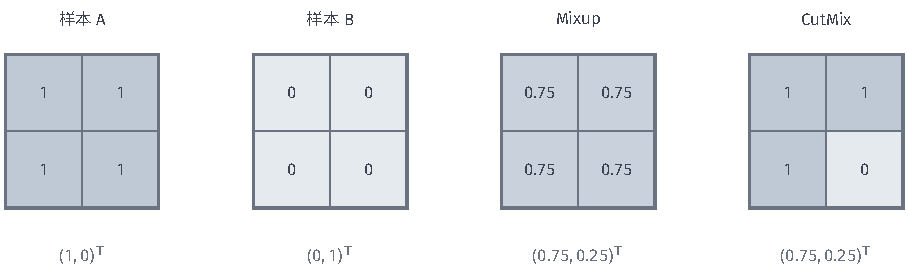
\includegraphics[width=153.793mm]{figures/05-neural-network-models/00-shared/tikz/generalization-mixing/figure.pdf}
  \caption{构造的两类$2\times2$输入及其混合。样本A各位置为1，目标为$(1,0)^{\top}$；样本B各位置为0，目标为$(0,1)^{\top}$。Mixup取$\lambda=0.75$，各位置变为0.75；CutMix替换右下位置，保留面积也为0.75。二者目标均为$(0.75,0.25)^{\top}$，但空间组织不同。教学数值用于比较混合机制，类别也是构造的。}
  \label{fig:generalization-mixing}
\end{figure*}

混合强度、配对与目标共同规定这份函数约束。插值缺少任务意义时，线性标签会引入错误监督；类别线索集中在小区域时，面积也可能误表其贡献。保留真实任务语义的验证样本用来检验这些构造是否改善原任务。

\section{模型侧的泛化控制}
\label{sec:generalization-constraints}

同一结构的未绑定版本允许各位置分别选择参数，共享与绑定将其中某些自由度合并；范数惩罚则保留参数范围，在损失中增加尺度或稀疏偏好。前者规定可选计算，后者评价候选，两条路线分别接到第\ref{sec:generalization-capacity}节的归纳偏置与范数复杂度分析（参考\BookSectionRef{sec:network-norm-bounds}{卷3《基础、理论与可信性》第8章“深度学习的可学习性”第8.2节“基于参数大小的可学习性”}）。

这里按主要作用位置区分模型侧与训练侧：固定结构及显式损失项放在本节，更新收缩、随机训练扰动和轨迹选择放在第\ref{sec:generalization-training-process}节。方法在数学上可以联系，例如普通SGD中的L2梯度等价于特定收缩；具体实现据改变目标还是改变更新确定其作用位置。

\subsection{参数共享与参数绑定}
\label{sec:generalization-parameter-sharing}

相同局部关系出现在多个位置时，可以让这些位置共同估计一份规则。第\ref{sec:generalization-capacity}节的结构偏好在这里体现为参数相等：自由度减少，各次使用的梯度汇到同一参数，也同时要求这些位置采用同一变换。\term{参数共享}（parameter sharing）让不同计算位置使用同一参数对象。卷积核跨位置复用，循环权重跨时间复用；每次使用都贡献梯度，更新时累积到同一对象。\term{参数绑定}（weight tying）则强调多个模块的参数被限制为相等或具有指定对应关系，硬绑定常通过共享实现。

例如，词表嵌入矩阵$\bm E\in\mathbb R^{v\times d}$的第$j$行表示词元$j$，输出隐藏状态为$\bm h\in\mathbb R^d$时，可以绑定输出矩阵，令分数$\bm z=\bm E\bm h+\bm b$。这里要求输出隐藏宽度与嵌入宽度相容，输入和输出词表也有一致对应；不相容时需投影或另外定义绑定范围。绑定让同一词元的输入表示与输出判别共享信息，也减少独立参数，但同时施加两种职责可由同一表示承担的假设。

若不希望强制相等，可加入$\lambda\lVert\bm\theta_A-\bm\theta_B\rVert_2^2/2$，鼓励两组参数接近。有限$\lambda$下它们仍是两个参数对象，这是一种软约束。共享规定相等的参数结构，软约束在仍可不同的参数之间增加代价。任务若需要不同位置采用不同规则，过强绑定可能妨碍拟合。

\subsection{参数范数惩罚}
\label{sec:generalization-norm-penalties}

多组参数都能拟合已有样本时，可以在训练损失之外给它们不同评价。范数惩罚增加参数尺度代价，再与输入和分类间隔一起分析风险（参考\BookSectionRef{sec:network-norm-bounds}{卷3《基础、理论与可信性》第8章“深度学习的可学习性”第8.2节“基于参数大小的可学习性”}）。\term{范数惩罚}（norm penalty）将学习目标改为
\begin{equation}
  \min_{\bm\theta}\ \hat R_S(\bm\theta)+\lambda\Omega(\bm\theta),
  \qquad\lambda\geq0\text{。}
  \label{eq:generalization-regularized-objective}
\end{equation}
常见选择为$\Omega=\lVert\bm\theta\rVert_1$或$\Omega=\lVert\bm\theta\rVert_2^2/2$。后者惩罚范数的平方，实践中常简称L2正则化。它惩罚参数幅度，L1在0附近的非光滑形状则可以促成精确的零参数。

\begin{example}[L1与L2的收缩不同]
  \label{ex:generalization-shrinkage}
  对标量教学目标$\tfrac12(w-a)^2$，加入$\lambda w^2/2$后，最优解为$w=a/(1+\lambda)$；加入$\lambda|w|$后，最优解为$w=\operatorname{sign}(a)\max(|a|-\lambda,0)$。例如$a=0.4,\lambda=0.5$时，前者为$0.4/1.5$，后者为0。两个解析最优解显示惩罚形状的作用；神经网络的实际稀疏结果还取决于其目标与非光滑求解方法。
\end{example}

如果要一起选择或去掉一组参数，可以采用$\Omega(\bm\theta)=\sum_g\lVert\bm\theta_g\rVert_2$，其中组$g$可能对应某个特征、神经元或通道，必要时再按组大小加权。组范数对整组是否为0产生偏好，与逐参数L1的稀疏形态不同。组的边界、是否重叠与大小权重共同定义实际惩罚。

L1与组范数的零点不可微，近端更新常能更直接处理其非光滑部分；L2则有梯度$\lambda\bm\theta$。参数尺度还受重参数化影响，例如ReLU网络中某层放大、下一层相应缩小可能保留函数但改变参数惩罚。相同函数因表示方式而有不同惩罚，分析和实现因而需要共同固定约束对象。系数及偏置、归一化参数是否参与，再决定额外代价作用于哪些自由度。

\section{训练侧的泛化控制}
\label{sec:generalization-training-process}

候选和显式损失确定后，还要选择何时停止、使用轨迹中的哪个状态、怎样更新以及施加什么扰动。这些选择改变同一数据上的学习过程，训练敏感性与选解偏好分别解释其中部分机制（参考\BookSectionRef{sec:algorithmic-stability}{卷3《基础、理论与可信性》第7章“一般学习的可学习性”第7.3节“算法稳定性与可学习性”}和\BookSectionRef{sec:implicit-bias}{卷3《基础、理论与可信性》第8章“深度学习的可学习性”第8.4节“基于参数梯度更新的可学习性”}）。验证风险用于比较学得候选的新数据表现。

下面先讨论停止、平均与优化器选择，再讨论权重衰减和随机扰动。权重衰减在更新中收缩参数，因此归入训练侧；Dropout及噪声按训练时的操作位置归类，也可以从随机计算的期望损失理解。期望损失联系目标，操作位置联系实现，两种描述可以用于同一方法。

\subsection{提前终止}
\label{sec:generalization-early-stopping}

训练损失还在下降时，验证损失可能已经开始升高。此时可以把沿同一数据训练的时长作为候选选择；对凸、光滑且Lipschitz的损失，在所需步长范围内采用独立均匀、有放回抽样的SGD时，训练时间和步长总量也会进入稳定性界（参考\BookSectionRef{sec:sgd-stability}{卷3《基础、理论与可信性》第7章“一般学习的可学习性”第7.4.3节“凸学习问题的随机梯度下降”}）。\term{提前终止}（early stopping）根据验证数据选择训练时刻，将训练轨迹上的参数位置当作候选模型。它需要规定评估指标、检查间隔、最小改善量和容忍窗口，并保存出现最佳验证表现时的参数。

例如，每训练一个轮次计算一次验证损失，若连续$p$次检查都没有超过阈值的改善，就停止并恢复已保存的最优参数。恢复参数与使用停止时刻的参数不同；继续训练还需相应恢复优化器和调度状态。随机验证增强、Dropout未关闭或BatchNorm模式错误，都可能让停止判断混入无关噪声。

图~\ref{fig:generalization-early-stopping}展示可能出现的曲线形状。真实曲线可能有多个起伏，短期变差后还可能改善。容忍窗口据噪声、调度与目标选择，决定要为后续改善等待多少计算。
\begin{figure}[htbp]
  \centering
  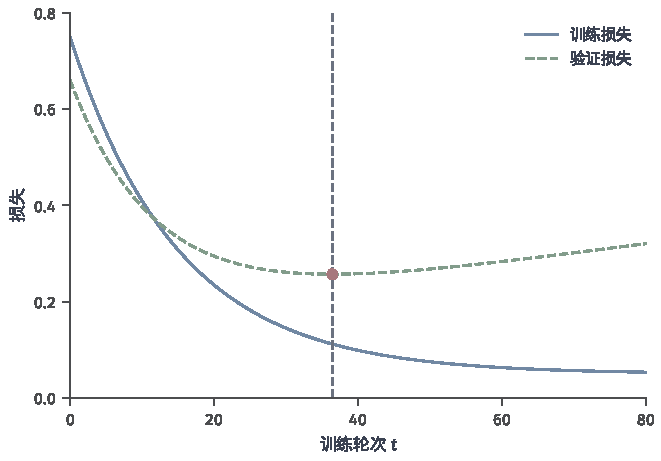
\includegraphics[width=105.412mm]{figures/05-neural-network-models/00-shared/matplotlib/generalization-early-stopping/figure.pdf}
  \caption{提前终止的示意曲线。训练损失取$0.05+0.7\exp(-t/15)$，验证损失取$0.16+0.5\exp(-t/12)+0.002t$，$t$为训练轮次。虚线标出该构造验证函数的极小点附近，说明继续拟合与验证表现可能分离；这些函数仅用于讲解，不是实验记录。}
  \label{fig:generalization-early-stopping}
\end{figure}

上述SGD稳定性分析先固定训练时长，再比较替换一个样本后的学习结果；步长总量和训练时间进入其上界，解释持续更新怎样累积对样本的依赖（参考\BookSectionRef{sec:sgd-stability}{卷3《基础、理论与可信性》第7章“一般学习的可学习性”第7.4.3节“凸学习问题的随机梯度下降”}）。根据验证数据选择停止时刻时，还需将这一选择过程纳入分析；实际停止仍在拟合进展和验证风险之间选择\scite{hardt2016sgd}

反复尝试停止策略时，验证集也在参与模型选择，所得方案可能适应这组数据的偶然差异。方案确定后再用最终测试评价。时间序列与持续感知还要模拟实际状态保留，让每个评价时刻只用当时可见的信息。

\subsection{参数平均}
\label{sec:generalization-weight-averaging}

更新噪声可能使训练后段的参数在附近波动，某个瞬时位置因而未必代表整段轨迹。参数平均综合这些位置，最后仍形成一个可直接推理的模型；平均位置的损失和验证表现确定这份综合是否合适。第\ref{sec:training-inexact-gradients}节说明了这些波动的来源。\term{指数移动平均}（exponential moving average, EMA）维护$\bar{\bm\theta}^{(t)}=\rho\bar{\bm\theta}^{(t-1)}+(1-\rho)\bm\theta^{(t)}$，$\rho\in[0,1)$。取初值为训练初始参数或当前参数可以避免零初值的缩小效应，$\rho$越大，对近期变化的响应越慢。推理时使用平均参数形成一个模型。

\term{随机权重平均}（stochastic weight averaging, SWA）选取训练后段的多个参数状态作算术平均。对已收集的$k$个状态，加入新状态$\bm\theta$时更新$\bar{\bm\theta}_{k+1}=k\bar{\bm\theta}_k/(k+1)+\bm\theta/(k+1)$。原始方案利用较大或周期性学习率采样训练后段区域，平均后若使用BatchNorm，还需按平均模型重新估计运行统计量\scite{izmailov2018swa}

参数坐标的平均要先经过网络计算，预测平均则组合已有输出。非线性映射通常不满足$f_{(\bm\theta_A+\bm\theta_B)/2}=(f_{\bm\theta_A}+f_{\bm\theta_B})/2$。同一轨迹附近的参数具有较一致的坐标含义，平均可能仍处在低损失区；独立模型的隐藏单元置换或尺度差异则可能把平均送到其他函数。

\begin{example}[等价网络的参数平均可以失效]
  \label{ex:generalization-parameter-average}
  取无偏置的两单元ReLU网络$f(x)=\operatorname{ReLU}(x)+\operatorname{ReLU}(-x)=|x|$。网络A的输入权重为$(1,-1)$，输出权重为$(1,1)$；网络B只交换两个隐藏单元，输入权重为$(-1,1)$，输出权重仍为$(1,1)$。两个网络的函数完全相同，但逐坐标平均后的输入权重为$(0,0)$，输出恒为0。预测平均仍给出$|x|$。
\end{example}

EMA和SWA在训练参数之外维护一份平均参数，推理使用这一个函数。它们综合同一轨迹，独立训练模型的预测集成则使用另一组函数；平均位置的偏差与实际验证风险仍据该模型评价。

\subsection{优化算法的隐式偏差}
\label{sec:generalization-implicit-bias}

同一目标有多个低损失解时，更新方向使轨迹倾向其中某些解。\term{隐式偏差}（implicit bias）描述学习过程形成的这种选择偏好；小批量无偏则描述梯度估计的期望。即使损失没有附加惩罚，线性和矩阵学习中的更新也可以产生特定偏好（参考\BookSectionRef{sec:implicit-bias}{卷3《基础、理论与可信性》第8章“深度学习的可学习性”第8.4节“基于参数梯度更新的可学习性”}）。

可分线性二分类提供一个明确结果：对$y_i\in\{-1,1\}$、无偏置线性得分和无显式惩罚的平均逻辑损失，在样本严格线性可分、采用满足收敛条件的固定正步长时，梯度下降使$\lVert\bm w\rVert_2$趋于无穷，方向趋向欧氏最大间隔分隔方向。这份经验逻辑损失的下确界为0，有限范数下达不到它；更新仍选择特定方向（条件与推导参考\BookSectionRef{sec:implicit-bias}{卷3《基础、理论与可信性》第8章“深度学习的可学习性”第8.4节“基于参数梯度更新的可学习性”}）\scite{soudry2018implicit}

\begin{example}[改变更新几何会改变选出的解]
  \label{ex:generalization-update-geometry}
  用一个训练样本拟合$w_1+2w_2=1$，目标为$\tfrac12(w_1+2w_2-1)^2$。从零初始化出发，足够小的固定步长梯度下降始终沿$(1,2)^{\top}$移动，收敛到$(1/5,2/5)^{\top}$，这是欧氏最小范数解。若改为固定预条件$\bm P=\operatorname{diag}(4,1)$，更新始终沿$(4,2)^{\top}$移动，则收敛到$(1/2,1/4)^{\top}$。两个解的训练误差都为0，后者最小化的是$\bm w^{\top}\bm P^{-1}\bm w$。未来数据若需要不同坐标承担不同作用，二者的风险也可能不同，哪种偏好适用要由未来输入与目标关系决定。
\end{example}

深度网络的选解偏好还随参数化、初始化、学习率、批量与时长改变，优化器比较因而需要固定网络与任务，并明确这些训练选择。Wilson等给出了自适应方法与GD／SGD选出不同解的构造，并在所研究的网络中观察到自适应方法训练更好而测试更差。这提供了比较非自适应与自适应更新的理由，结论限于相应设置\scite{wilson2017adaptive}

Choi等发现，优化器排名随超参数搜索范围和调节预算改变。比较时给不同方法各自调节参数，并使搜索预算相当；相同学习率数值在不同更新规则下可以产生不同位移。AdamW又含解耦衰减，更新方向与参数收缩都进入实际方案\scite{choi2020optimizers}

下面的比较过程用来检验当前任务中的选解差异：
\begin{enumerate}
  \item 固定网络、数据划分、增强与损失，以带动量SGD和AdamW作为两种候选。已有训练方案能稳定拟合时，先保留其为基准；更换优化器是检验不同更新几何的一种方式。
  \item 分别调节学习率、调度、动量或矩系数，以及适用的衰减系数。给两类候选相当的搜索与训练预算，记录达到目标训练损失的成本和验证表现。
  \item 联合阅读训练与验证曲线。训练误差仍高时，先排查第\ref{chap:neural-network-training}章的优化困难；训练相近而验证明显不同，才更便于判断不同训练规则带来的预测差异。固定时间预算的表现也应单独报告，因为慢方法可能尚未完成拟合。
  \item 对有希望的配置使用多个随机种子复核，再用验证结果选择。停止时刻、批量和参数平均也会改变轨迹，可以分别作控制实验；方案确定之后再做最终测试。
\end{enumerate}

代表性验证数据和多次训练支持某配置时，可以在该任务上采用它，结论随这份网络、数据和预算保留。中途从AdamW切到SGD会改变方向形成和状态含义；学习率、旧状态的丢弃或转换及切换时刻共同定义新方案，再由验证比较其效果。

参数平坦性描述指定坐标与扰动尺度内的损失变化，保持函数不变的重缩放也可以改变这一曲率。用它评价选解时，需固定坐标和尺度，或明确处理重参数化的方法，再将指标与当前任务的未来风险比较\scite{dinh2017sharp}

\subsection{邻域最坏损失与SAM}
\label{sec:generalization-sam}

在当前参数附近移动后损失迅速升高时，可以要求模型连同该邻域一起保持较低损失。指定坐标、范数和正半径后，用邻域内最大的损失作为外层目标。\term{锐度感知最小化}（sharpness-aware minimization, SAM）考虑
\begin{equation}
  \min_{\bm w}\ \max_{\lVert\bm\epsilon\rVert_2\leq\rho}
    \mathcal L(\bm w+\bm\epsilon)\text{。}
  \label{eq:generalization-sam}
\end{equation}
对内层目标在$\bm w$处作一阶近似且$\nabla\mathcal L(\bm w)\ne\bm0$时，欧氏球上的近似最大化点为
\[
  \bm\epsilon^\star
  =\rho\frac{\nabla\mathcal L(\bm w)}
              {\lVert\nabla\mathcal L(\bm w)\rVert_2}\text{。}
\]
随后在扰动点计算梯度，却把更新施加到原参数：$\bm w^+=\bm w-\eta\nabla\mathcal L(\bm w+\bm\epsilon^\star)$。图~\ref{fig:generalization-sam}把这两个步骤分开：红箭头寻找邻域内的高损失方向，绿色箭头读取该处梯度，却移动原参数。实际小批量实现常用同一批数据完成两次前后向；零梯度时的处理、归一化层状态、扰动范数和参数分组共同定义这两次计算。
\begin{figure*}[htbp]
  \centering
  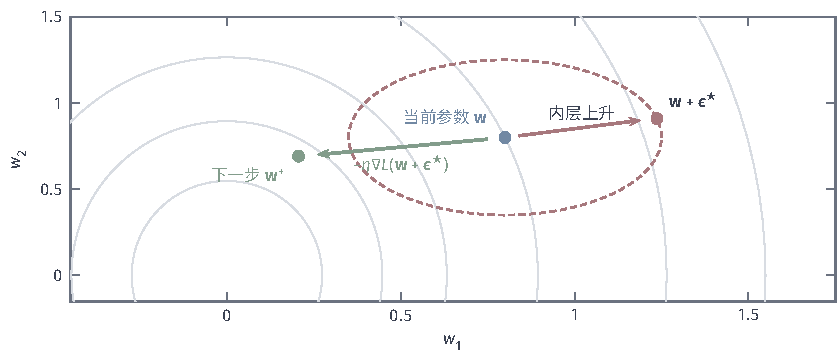
\includegraphics[width=142.275mm]{figures/05-neural-network-models/00-shared/tikz/generalization-sam/figure.pdf}
  \caption{SAM一次近似更新的几何过程。灰线为教学目标$L(\bm w)=(4w_1^2+w_2^2)/2$的等高线，红色虚线是以当前参数为中心、半径$\rho=0.45$的扰动邻域。红箭头沿当前梯度的一阶近似到达边界高损失点，绿色箭头使用该扰动点的梯度更新原参数。图示说明两次梯度读取及更新的位置；内层只采用一阶近似，泛化效果另在任务上评价。}
  \label{fig:generalization-sam}
\end{figure*}

SAM在指定参数坐标和范数下改变邻域目标，重参数化也会改变同一函数的扰动集合。$\rho$很小时更新接近普通梯度，较大时一阶近似可能失准或妨碍拟合。这里扰动参数，输入鲁棒训练则扰动样本，两者评价的邻域不同。两次前后向的成本、训练拟合与独立验证风险一起说明该目标是否适合当前任务\scite{foret2021sam}

\subsection{权重衰减}
\label{sec:generalization-weight-decay}

当前位置的梯度给出数据损失方向，还可以在同一次更新中缩小参数幅度。\term{权重衰减}（weight decay）直接加入这种参数收缩；通常将学习率与衰减系数的乘积限制在零与一之间。第\ref{sec:training-optimizers}节的方向、尺度与历史状态共同决定它是否等价于损失中的范数惩罚。对无动量的普通SGD，L2惩罚更新为
\begin{equation}
  \bm\theta^{(t)}=\bm\theta^{(t-1)}-
    \eta_t(\bm g^{(t)}+\lambda\bm\theta^{(t-1)})
  =(1-\eta_t\lambda)\bm\theta^{(t-1)}-\eta_t\bm g^{(t)}\text{。}
  \label{eq:generalization-sgd-weight-decay}
\end{equation}
因而在相同参数范围及系数约定下，L2惩罚与学习率乘以$\lambda$的收缩等价。若所谓“衰减系数”直接表示每步乘法系数，就还需对应学习率；加入动量后，惩罚是否进入缓冲会改变下一步方向，等价关系据该实现重新对应。

对预条件矩阵$\bm P^{(t)}$，惩罚项进入梯度后产生$-\eta_t\lambda\bm P^{(t)}\bm\theta$，而解耦收缩产生$-\eta_t\lambda\bm\theta$。二者通常不同，Adam中惩罚还可能进入一阶、二阶矩统计。\term{AdamW}将衰减从自适应梯度更新中分离，其基本更新为
\begin{equation}
  \bm\theta^{(t)}=(1-\eta_t\lambda)\bm\theta^{(t-1)}-
    \eta_t\frac{\hat{\bm m}^{(t)}}{\sqrt{\hat{\bm v}^{(t)}}+\epsilon}\text{，}
  \label{eq:generalization-adamw}
\end{equation}
这里矩统计来自数据损失梯度，具体计算见式\eqref{eq:training-adam}\scite{loshchilov2019adamw}

衰减通过多步乘积发生，学习率调度、更新次数和是否排除部分参数都会改变总收缩量。解耦项按原参数直接收缩，预条件后的惩罚梯度则使用另一个方向。比较强度时同时固定更新规则与系数含义。

\subsection{Dropout}
\label{sec:generalization-dropout}
\label{sec:generalization-stochastic-regularization}

分类器若总依赖同一组中间特征共同出现，可以在训练中随机屏蔽其中一些，要求剩余特征仍参与预测。共享参数由这些随机计算共同训练，因而接受不同可用路径下的监督。\term{Dropout}在训练时随机屏蔽部分激活，使网络在不同的可用特征子集上完成同一任务。设隐藏表示为$\bm h$，各元素独立保留概率为$q\in(0,1]$，$m_j\sim\operatorname{Bernoulli}(q)$。常见的反向缩放形式为
\begin{equation}
  \tilde h_j=\frac{m_j}{q}h_j,\qquad
  \mathbb E[\tilde h_j\mid\bm h]=h_j,\qquad
  \operatorname{Var}(\tilde h_j\mid\bm h)=\frac{1-q}{q}h_j^2\text{。}
  \label{eq:generalization-dropout}
\end{equation}
训练时除以$q$，常规推理时关闭屏蔽并直接使用$\bm h$。另一约定在训练时不缩放、推理时乘$q$，两者必须与实现一致。这里$q$为保留率，有些接口使用的是失活率$1-q$\scite{srivastava2014dropout}

训练目标包含对掩码的期望$\mathbb E_{\bm m}\ell(f_{\bm\theta,\bm m}(\bm x),y)$。各掩码产生的子网络共享参数，梯度共同更新同一组对象。隐藏表示的期望虽被保持，完整非线性映射一般不满足$\mathbb E_{\bm m}f_{\bm\theta,\bm m}=f_{\bm\theta}$；无掩码推理提供确定计算，对随机网络平均的解释采用近似。

图~\ref{fig:generalization-dropout}展示同一隐藏层的一个掩码样本。被屏蔽单元的输入参数仍保留，后续批量可以重新启用该路径。较低$q$增加扰动和方差，也可能损害拟合。BatchNorm与Dropout组合时，还需关注随机激活对运行统计的影响；序列模型中跨时间独立采样或共享掩码，则具有不同扰动结构。
\begin{figure}[htbp]
  \centering
  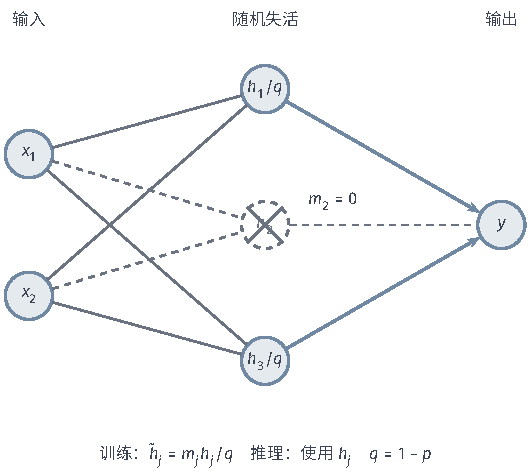
\includegraphics[width=89.793mm]{figures/05-neural-network-models/00-shared/tikz/generalization-dropout/figure.pdf}
  \caption{一个三单元隐藏层的构造性Dropout示意。中间单元保留浅灰$h_2$轮廓并标出$m_2=0$，表示本批屏蔽的单元仍保留在模型中；灰色虚线为本次不参与前向计算的路径。底部公式带明确区分保留概率$q=1-p$与丢弃概率$p$，并给出inverted Dropout在训练时除以$q$、推理时无需再缩放的约定。}
  \label{fig:generalization-dropout}
\end{figure}

\subsection{结构化随机失活}
\label{sec:generalization-structured-dropout}

随机扰动应覆盖模型真正依赖的信息单位；若重复线索能从邻近位置轻易补回，逐元素屏蔽施加的约束就较弱。结构化随机失活根据网络结构选择连接、通道、空间块或整层作为屏蔽对象，使扰动粒度与第\ref{sec:training-connections}节的结构组织对应。

\term{DropConnect}对权重连接采样掩码，令$\tilde{\bm W}=\bm M\odot\bm W$，随后再计算激活；Dropout则直接作用于激活。基本训练与推理的缩放、分布近似应按各自约定处理，两种失活的随机函数不相同\scite{wan2013dropconnect}

\term{空间Dropout}（spatial dropout）在一个通道的所有空间位置使用同一掩码，削弱网络对某个整通道特征的依赖。\term{DropBlock}随机屏蔽特征图中连续的空间块，干扰局部邻域可提供的重复信息。多个块会重叠，边界也截掉部分位置，因此块中心的采样概率与最终元素失活比例需要分别计算\scite{ghiasi2018dropblock}

\term{随机深度}（stochastic depth）对残差分支随机启用或绕过，让训练时经过的有效深度变化。一个期望保持的实现写为$\bm h^{(l+1)}=\bm h^{(l)}+(m_l/q_l)F_l(\bm h^{(l)})$，$m_l\sim\operatorname{Bernoulli}(q_l)$，推理时使用全部分支。原始方法也可将缩放放在推理阶段；是否真正跳过被屏蔽分支的计算影响训练时间\scite{huang2016stochasticdepth}

连接、通道、空间块和整层使不同信息共同失活。小对象、窄通道或缺少恒等路径时，大块屏蔽可能直接去掉任务证据。保留概率、作用位置与掩码共享范围共同确定扰动，再据实际结构和验证结果选择其强度。

\subsection{噪声注入}
\label{sec:generalization-noise}

除保留或屏蔽之外，还可以连续改变表示或参数，在规定扰动分布下训练其平均表现。完整网络的参数扰动形成预测器分布，可以用从中抽取网络的期望损失评价（参考\BookSectionRef{sec:parameter-distributions}{卷3《基础、理论与可信性》第8章“深度学习的可学习性”第8.5节“基于参数分布的可学习性”}）。\term{噪声注入}（noise injection）在训练中使用$\tilde{\bm h}=\bm h+\bm\epsilon$或$\tilde{\bm\theta}=\bm\theta+\bm\epsilon$，其中噪声的均值、协方差和采样范围需要明确。输入噪声属于数据增强的一种，中间表示噪声改变后续计算，参数噪声则同时影响所有使用该参数的位置。

对足够光滑的目标函数和小幅零均值噪声，二阶展开给出局部近似
\begin{equation}
  \mathbb E_{\bm\epsilon}[\mathcal L(\bm\theta+\bm\epsilon)]
  \approx\mathcal L(\bm\theta)+\tfrac12
      \operatorname{tr}(\bm\Sigma\nabla^2\mathcal L(\bm\theta))\text{，}
  \label{eq:generalization-noise-expansion}
\end{equation}
其中$\bm\Sigma=\mathbb E[\bm\epsilon\bm\epsilon^{\top}]$。噪声幅度与光滑条件控制余项，协方差与当前Hessian共同决定二阶项；非凸区域的负曲率还可能使该项为负。

一个可精确核查的特殊情况是线性回归。给定当前样本，对预测$\bm w^{\top}\bm x$、平方损失及输入噪声$\mathbb E\bm\epsilon=\bm0$、$\mathbb E\bm\epsilon\bm\epsilon^{\top}=\sigma^2\bm I$，有
\begin{equation}
  \mathbb E\tfrac12[y-\bm w^{\top}(\bm x+\bm\epsilon)]^2
  =\tfrac12(y-\bm w^{\top}\bm x)^2+\tfrac{\sigma^2}{2}\lVert\bm w\rVert_2^2\text{。}
  \label{eq:generalization-linear-noise}
\end{equation}
零均值消去交叉项，协方差决定额外二次项。这份精确联系来自线性预测、平方损失与输入噪声，改变模型、损失或注入位置后，期望目标需按新计算展开。

Dropout也可理解为一种乘性噪声：$\tilde h_j=h_j+[m_j/q-1]h_j$，条件均值为0、方差与$h_j^2$成比例。它与加性高斯噪声的分布和尺度不同。噪声是否符合任务中合理的变化，决定了对局部邻域的约束是否有意义；系统性错误标签或数据泄漏则仍需修正监督与数据组织。

\section{模型集成}
\label{sec:generalization-ensembles}

若不同训练过程保留了不同预测误差，可以通过组合预测减少其中部分波动。第\ref{sec:generalization-solution-selection}节的解差异在这里进入组合，成员质量与误差相关性共同决定效果。

\subsection{装袋法（Bagging）}
\label{sec:generalization-bagging}

\term{装袋法}（bootstrap aggregating, Bagging）从训练集多次自助重采样，分别训练成员，再组合预测，\BookSectionRef{sec:ensemble-bagging-bootstrap}{卷4《模型：经典模型》第6章“集成学习”第6.1.1节“Bagging”}给出采样机制。变化的样本集合形成不同解，预测组合尝试减弱单次采样的影响。这里也关心学习过程的抽样敏感性，算法稳定性则在指定假设下分析替换样本对损失的影响（参考\BookSectionRef{sec:algorithmic-stability}{卷3《基础、理论与可信性》第7章“一般学习的可学习性”第7.3节“算法稳定性与可学习性”}）。用神经网络作为成员时，仍需保持相同的输出语义：回归平均数值预测，分类可平均类别概率或投票；概率平均通常不等于先平均分数再做Softmax。组合规则见\BookSectionRef{sec:ensemble-members-combination-output}{卷4《模型：经典模型》第6章“集成学习”}\scite{breiman1996bagging}

对含$n\geq1$条记录的训练集独立、有放回地抽取$n$次，指定记录未被抽中的概率为$(1-1/n)^n$，随$n$增大趋近于$e^{-1}$。袋外预测只组合没有抽到该记录的成员；它为这条记录保留相应的训练隔离，但不能替代超参数选择后的独立测试。这两项计算可参考\BookEquationRef{eq:ensemble-oob-probability}{卷4《模型：经典模型》第6章“集成学习”第6.1.1.1节“自助样本与聚合预测”}与\BookEquationRef{eq:ensemble-oob-prediction}{卷4《模型：经典模型》第6章“集成学习”第6.1.1.1节“自助样本与聚合预测”}。神经网络的超参数和成员由验证选择，相关数据再按实际抽样单位重采样。例如按主体抽取体现主体变化，按窗口抽取则体现另一种随机过程。

集成收益还取决于成员之间共享多少波动。\BookEquationRef{eq:ensemble-correlated-variance}{卷4《模型：经典模型》第6章“集成学习”第6.5.1节“成员质量、错误依赖与多样性”}在固定输入、等方差和等相关条件下，描述标量预测平均的方差，随机性来自训练集抽取、重采样及训练过程。共同波动在平均中继续保留，偏差还由成员的期望预测决定。这份标量预测方差公式解释波动，分类零一风险则还取决于目标与决策边界。

\subsection{基于训练随机性的集成}
\label{sec:generalization-randomness-ensemble}

初始化、数据次序、增强和随机失活在同一训练集上也能形成不同预测函数，来源见第\ref{sec:generalization-solution-selection}节。使用这些训练选择构建集成时，差异来自过程，成员可以使用相同原始样本。袋外集合则需要装袋法中未抽中的样本这一数据组织。

成员质量与差异共同进入组合。在关键输入上系统性错误的模型可能拖低预测，几乎相同的模型则保留共同误差。单模型表现、预测分歧与组合权重由同一验证方案比较，确定成员后再做最终测试。

集成通常增加训练和推理成本。$M$个相同规模网络若顺序运行，模型计算量约为单个的$M$倍；并行运行可以降低部分等待时间，却需要更多设备或存储。第\ref{sec:generalization-weight-averaging}节的参数平均形成一个模型，预测集成则保留多个模型；前者在平均参数上重新计算，后者组合已有输出，函数与部署成本都可能不同。成员数与组合规则据任务质量、延迟和资源预算共同选择。

\section{本章小结}
\label{sec:generalization-summary}

相同训练拟合可以依赖不同线索，未来使用时的风险因而需要连同数据覆盖、结构偏好与选解过程判断。同分布新样本、场景变化和持续状态各有评价条件，数据划分据实际使用方式组织。

增强把任务允许的变化写进经验目标，参数共享与范数惩罚引入结构和尺度偏好，权重衰减通过更新收缩参数，随机失活与噪声约束受扰动的计算，停止时刻和参数平均改变轨迹上的解选择，集成则利用多个预测的差异。组合时各自条件仍起作用：增强保持任务语义，约束保留所需规律，参数平均保持坐标对应，集成成员提供合适差异。复杂度、稳定性与隐式偏差解释其中不同环节，符合使用场景的验证与独立测试再检验完整方案。

\paragraph{扩展阅读}
Goodfellow等教材第7章讨论显式与隐式正则化；Mixup原论文展示如何把样本间的插值约束加入训练。阅读时可将增强的任务语义、更新路径与预测评价接在一起，辨认各结果使用的数据与条件\scite{goodfellow2016,zhang2018mixup}

